\documentclass[twoside]{report} % double side
%\documentclass[]{report} % single side

\usepackage[dvips]{graphicx}
%\usepackage{epsfig}
% --- Papierformat soll A4 sein
%\usepackage{a4}
%\usepackage{a5}
% --- Anzeigen aller \label und \ref -Kommandows
%     (Bei Bedarf aktivieren durch Entfernen des %)
%\usepackage{showkeys}
% --- Verwenden der deutschen Trennmuster
%%\usepackage{german}
% --- Trennmuster fuer Ausnahmefaelle
\hyphenation{me-cha-nik}
\hyphenation{pro-per-ties}


% --- Unterstuetzen von deutschen Umlauten
%\usepackage[ansi]{umlaute}
\usepackage[utf8]{inputenc}   %--->for ubuntu linux


% Absaetze nicht einruecken
\setlength{\parindent}{0pt}
\setlength{\parskip}{5pt plus 2pt minus 1pt}
\usepackage{float,color,latexsym, epic,eepic,rotating}
\usepackage{fheading}           % Seitenkopf gestalten
\usepackage{amssymb, amsmath}
\usepackage{epsfig, epic, eepic}
\usepackage{bm}
\usepackage[usenames,dvipsnames]{pstricks}


% Who added this, please comment
\makeatletter
\renewcommand\thefigure{\thesection.\arabic{figure}}
\makeatother            
\usepackage[version=3]{mhchem}
\usepackage{booktabs}
\usepackage{units}
\usepackage{subfigure}
\usepackage{caption}
\captionsetup{format=hang,justification=raggedright,justification=justified}
\usepackage{color}
\usepackage[hyperref, dvips, colorlinks, linkcolor=black,
                 citecolor=black, urlcolor=black]{hyperref}
%\usepackage{hypdvips}
\usepackage{ltablex}  %to generate automatic line breaks in table ( compination of landscape and tabularx)
\usepackage{longtable}
\usepackage{lscape}% to get table in landscape format

\usepackage{paralist}
\usepackage{arydshln}

\usepackage{pst-grad} % For gradients
\usepackage{pst-plot} % For axes
\pagestyle{fancy}
\lhead[\fancyplain{}{\footnotesize\textsf\thepage}]%
      {\fancyplain{}{\footnotesize\textsf\rightmark}}
\rhead[\fancyplain{}{\footnotesize\textsf\leftmark}]%
      {\fancyplain{}{\footnotesize\textsf\thepage}}
\cfoot{}

%\renewcommand{\arraystretch}{1.2}

% Makros
% general
\newcommand{\D}{\displaystyle}
%%\newcommand{\Vec}[1]{{\bf \bar{#1} }}
\newcommand{\Boldmath}[1]{\mbox{\boldmath ${#1}$ \unboldmath}}
%%\newcommand{\boldsymbol}[1]{\mbox{\boldmath ${#1}$ \unboldmath}}
% geometry
\def \VolSol {V}
\def \AreaSol {A}
\def \Domain {\Omega}
% fluid flow
\def \Phase {\gamma}
\def \VolumetricFraction {\epsilon}
\newcommand{\p}{\partial}
\newcommand{\PiezoHead}{p/g\rho+z}
\def \Viscosity {\mu}
\def \Pressure {p}
\def \Perm {k}
\def \Source {Q}
\def \Porosity {n}%{\theta^f}
\def \DensSolid {\rho^s}
\def \DensFluid {\rho^f}
\def \Density {\rho}
\def \DarcyVelo {q}
\def \DarcyVeloVector {\mathbf\DarcyVelo}
\def \Gravity {g}
\def \GravityVector {\mathbf{g}}
\def \Stor {S}
\def \FluidCompressibility {\beta_p}
\def \ThermalExpansionCoefficient {\beta_T}
%
\def \PermRelP {k_{\mbox{\footnotesize rel}}}
\def \PermTensorRelComp {k_{\alpha\beta}^0}
\def \PermTensor {\mathbf{k}}
\def \FluidMassSourceP {Q_\rho^p}
\def \Saturation {S}
\def \MoistureContent {\theta}
\def \CapillaryPressure {\Pressure_{\mbox{\footnotesize c}}}
\def \PermRelS {k_{\mbox{\footnotesize rel}}}
\def \SaturationEff {\Saturation_{\mbox{\footnotesize eff}}}
\def \SaturationMax {\Saturation_{\mbox{\footnotesize max}}}
\def \SaturationRes {\Saturation_r}
\def \GasVelocityVector {{\mathbf{v}}^{g}}
\def \WaterVelocityVector {{\mathbf{v}}^{w}}
\def \VelocityVector {{\mathbf{v}}}
% deformation
\newcommand{\U}{u}
\newcommand{\Stress}{\mbox{\boldmath $\sigma$}}
\newcommand{\Shear}{\mbox{\boldmath $\tau$ \unboldmath}}
\def \Treps {\varepsilon}
% mass transport
\def \Conc {C}
\def \Solubility {C_s}
\def \VeloDisso {Rd}
\def \Diffusion {D}
% heat transport
\def \TLatentB {T_{l1}}
\def \TLatentE {T_{l2}}
\def \Temperature {T}
\def \HeatCapacity {c}
\def \HeatConductivity {\lambda}
\def \LatentHeat {L_0}
\def \Enthalpy {H}
% numerics
\newcommand{\Ne}{\frac{\alpha\Delta t}{\Delta x^2}}
\newcommand{\WF}{\omega}
\newcommand{\IF}{\phi}
\newcommand{\SF}{N}
\newcommand{\SFV}{{\mathbf\SF}}
\def \SFVPressure {\SFV_p}
\newcommand{\JacOneD}{[J_{1D}]}
\newcommand{\JacTwoD}{[J_{2D}]}
\newcommand{\JacInvOneD}{[J_{1D}^{-1}]}
\newcommand{\JacInvTwoD}{[J_{2D}^{-1}]}
\newcommand{\SFGradOneD}{[\nabla_r \SF]}
\newcommand{\SFGradTwoD}{[\nabla_{rs} \SF]}
\newcommand{\WFV}{\mbox{\boldmath $\omega$ \unboldmath}}
\newcommand{\IFV}{\mbox{\boldmath $\phi$ \unboldmath}}
\def \PressureVec {{\mathbf\Pressure}}
\def \SaturationVec {{\mathbf\Saturation}}
\def \TemperatureVec {{\mathbf\Temperature}}



%stresses
\def\Str {{\boldsymbol{\sigma}}}
\def\Strsc {{\sigma}}
\def\Streff {{\boldsymbol{\sigma}\!\!'}}
\def\Streffsc {{\sigma}^{\mathrm{S}}}
\def\Streffu {{\boldsymbol{\sigma}}_{\mathrm{S}}}
\def\Streffusc {{\sigma}_{\mathrm{S}}}
\def\StressSolid {{\boldsymbol{\sigma}\!\!}^s}
\def\StressFluid {{\boldsymbol{\sigma}\!\!}^w}

\def\CauStr {{\mathbf T}}

%Factors for effective stresses
\def \FacBulk {\alpha}
\def \FacEff {\alpha'}

%strains
\def\Stra {\boldsymbol{\varepsilon}}
\def\Strasc {\varepsilon}
\def\Strael {{\boldsymbol{\varepsilon}}^{el}}
\def\Straelsc {{\varepsilon}^{el}}
\def\Strain {{\boldsymbol{\varepsilon}\!\!}^{in}}
\def\Strainsc {\varepsilon^{in}}
%displacements
%\def\Disp {{\boldsymbol{u}}^s}
%\def\Disp {{\mathbf u}^s}
\def\Disp {{\mathbf u}}
\def\Dispsc {{\rm u}^s}
%\def\Dispu {{\boldsymbol{u}}_s}
\def\Dispu {{\mathbf u}_s}
\def\Dispusc {\rm u_s}

\def\Cten {\bf C}

%Testfunction  = Linear combination of the basis elements
\def\TF {N}
\def\TFV {\mathbf{\TF}}
\def\TFDisp {\eta^{u}}
\def\TFVDisp {\TFV_u}
\def\TFPressure {\eta^{p}}


\def \WFV {\boldsymbol{\WF}}
\def \IFV {\boldsymbol{\IF}}

\def \GradWFT {\mathbf L}
\def \GradIF {\boldsymbol\phi}

\def \BDom {\Gamma}
\def \Dom {\Omega}
\def \BApDom {\hat{\Gamma}}
\def \ApDom {\hat{\Omega}}
\def \BElDom {\Gamma^{e}}
\def \ElDom {\Omega^{e}}

\def \XV {\mathbf x}

%volume fraction
\def \VolFrf {n^{\mathrm{F}}}
\def \VolFrs {n^{\mathrm{S}}}

%Volume strain
\def \VolStrain {\varepsilon}
\def \Treps {\VolStrain}
\def \VolStrainIn {\varepsilon_{in}}
\def \VolStrainEl {\varepsilon_{el}}

%Fluid pressure
\def \FluidPressure {p}

%fluid Properties
\def \DynVisc {\mu}


%Storativity
\def \Storativity{S}

%Bulk moduli
\def \BulkMFluid {K_f}
\def \BulkMGrain {K_S}
\def \BulkMTang  {K_T}

%Hook's Law
\def \LambdaSolid {\lambda}
\def \ShModSolid {G}
\def \PoissRatio {\nu}

%Fluid motion
\def \VelFluid {{\mathbf v}^f}
\def \VelFluidu {{\mathbf v}_f}
\def \RelVel {{\mathbf w}^f}
\def \RelVelu {{\mathbf w}_f}
\def \VolAvRelVel {{\mathbf q}}
\def \VolAvVelFluid {{\mathbf v}^F}
\def \VolAvVelFluidu {{\mathbf v}_F}


%Solid motion
\def \VelSolid {{\mathbf v}^s}
\def \VelSolidu {{\mathbf v}_s}

%Acceleration
\def\Acc {{\mathbf a}}
\def\AccSolid {{\mathbf a}_s}
\def\AccFluid {{\mathbf a}_f}

%Partial densities
\def \PartDensSolid {\rho^{\rm S}}
\def \PartDensFluid {\rho^{\rm F}}

\def \DensBody {\rho_{b}}


%MK special
\newcommand {\Tensor} {\mbox}
%\newcommand {\Tensor} {\fbox}



%OK new
\def \BiotConstant {\alpha}
\def \SolidBulkModulus {K_s}
\def \SolidVelocityVector {{\mathbf{v}}^{s}}
\def \SolidVelocityComponent {v^s}
\def \GradOperator {{\bf L}}
\def \UnitOperator {{\bf m}}


\newcommand {\Unit} {\mbox}
\newcommand {\DoNothing}[1] {}

%math-symbols
\def \Id {{\,\rm d}}      % d des Integrals
\def \Dd {{\rm d}}        % d des Differentials
\def \div {{\rm \,div\,}}      % div
\def \grad {{\rm \,grad\,}}      % grad
\def \Grad {{\rm \,Grad\,}}      % Grad
\def \tr {{\rm \,tr}}           % tr

%Tensor notation
\def  \Isec  {\boldsymbol {\rm 1}}
%\def  \Ifourth {\boldsymbol{\rm 1\kern-.25em I}}
\def  \Ifourth {\boldsymbol{\rm I}}


%C-Tensor
\def  \CC    {{{\rm\kern.24em
               \vrule width.04em
               height1.6ex depth0.05ex
               \kern-0.4em C}}}

\def \BodyForce {\mathbf b}
\def \GravityAcc {\mathbf g}

\def \where {\mbox{where }}


\DeclareFontFamily{U}{euc}{}
\DeclareFontShape{U}{euc}{m}{n}{<-6>eurm5<6-8>eurm7<8->eurm10}{}%
\DeclareSymbolFont{AMSc}{U}{euc}{m}{n}
\DeclareMathSymbol{\usigma}{\mathord}{AMSc}{27}

\numberwithin{figure}{section}
\numberwithin{equation}{section}
\numberwithin{table}{section}

% Use a new style for remarks
%\theoremstyle{remark}
\newtheorem{rmk}{\textbf {Remark}}
\newtheorem{lemma}{Lemma}
\newtheorem{prop}{Proposition}
\newtheorem{proof}{Proof}
\numberwithin{lemma}{section}
\newtheorem{axiom}{Axiom}
\numberwithin{axiom}{section}

\providecommand{\sembrack}[1]{[\![#1]\!]}
\providecommand{\pD}[2]{\dfrac{\partial #1}{\partial #2}}
\providecommand{\oD}[2]{\dfrac{\mathrm d #1}{\mathrm d  #2}}
\providecommand{\abs}[1]{\lvert #1 \rvert}
%%\providecommand{\abs}[1]{\left\lvert #1 \right\rvert}
\providecommand{\norm}[1]{\left\lVert #1 \right\rVert}
\newcommand{\od}{\mathrm d}

%%%
\newcommand{\js}{\mathscr S}
%%%
%%material index
\newcommand{\pl}{\scriptscriptstyle \mathrm p}
\newcommand{\el}{\scriptscriptstyle \mathrm e}

%%Geometry
\newcommand{\Point}{ \bm x}


%%Displacement field
\providecommand{\Stress}{ \bm \sigma}
\newcommand{\inPStress}{ \Stress_{\imath}} %%% in-plane stress
\newcommand{\stress}{ \sigma}
\newcommand{\devStrs}{\bm s}
\providecommand{\StrainT}{ \bm \epsilon}
\newcommand{\strain}{ \epsilon}
\providecommand{\Disp}{\mathbf u}
\newcommand{\disp}{u}
\newcommand{\vel}{\bf v}
\newcommand{\per}{\mathbf k}
\newcommand{\grv}{\mathbf g}
%%Plasticity
\newcommand{\yld}{ f}
\newcommand{\ppo}{ g}
\newcommand{\pHard}{\mathcal H}
\newcommand{\CT}{\mathbb C}
\newcommand{\DT}{\mathbb D}
\newcommand{\EM}{{\bm C}^{\el}}
\newcommand{\PM}{{\bm C}^{\pl}}
\newcommand{\EPM}{{\bm C}^{\el\pl}}
\newcommand{\mEM}{{\bm D}^{\el}}
\newcommand{\mPM}{{\bm D}^{\pl}}
\newcommand{\mEPM}{{\bm D}^{\el\pl}}
\newcommand{\rdl}{\dot \lambda}
\newcommand{\dl}{\lambda}
\newcommand{\dens}{\rho}
\newcommand{\mnote}{\scriptscriptstyle M}

%%Flow
\newcommand{\densc}{\dens^{\gamma}}
\newcommand{\presc}{p^{\gamma}}
\newcommand{\pres}{p}
\newcommand{\sat}{S}
\newcommand{\Satc}{S^{\gamma}}
\newcommand{\RelKa}{k_{rel}}
\newcommand{\RelK}{k^{\gamma}_{rel}}
\newcommand{\poro}{n}
%%\newcommand{\Fluxf}{\mathbf{v}_{\scriptscriptstyle f}}
\newcommand{\Fluxf}{\mathbf{q}_{\scriptscriptstyle w}}
\newcommand{\Fluxv}{\mathbf{q}_{\scriptscriptstyle v}}
\providecommand{\perm}{ \mathbf k}
\newcommand{\asup}[2]{#1^#2}
\newcommand{\asub}[2]{#1_#2}
\newcommand{\supsub}[3]{{#1}^{#2}_{#3}}
\newcommand{\FlxDf}{\mathbf{J}}
\newcommand{\Sat}{S}

\newcommand{\pn}{\mathbf p}
\newcommand{\pnote}{\scriptscriptstyle f}
%%Heat
\newcommand{\HC}{C_p}
\newcommand{\Flux}{\mathbf{q}}
\newcommand{\Tn}{\mathbf T}
\newcommand{\Tnote}{\scriptscriptstyle T}

%%%FEM
\newcommand{\test}{w}
\newcommand{\Test}{\bm w}
\newcommand{\TestS}{\mathcal V}
\newcommand{\sh}{N}
\newcommand{\Sh}{{\bm N}}
\newcommand{\Mass}{{\mathbf M}}
\newcommand{\Lap}{{\mathbf K}}
\newcommand{\rhs}{{\mathbf f}}

%%Math
\newcommand{\IntD}[1]{{\int}_{\Omega}#1\,\mathrm{d} \Omega}
\newcommand{\intD}{{\int}_{\Omega}}
\newcommand{\intB}{{\int}_{\Gamma}}
\newcommand{\dDom}{\,\mathrm{d} \Omega}
\newcommand{\dBdry}{\,\mathrm{d} \Gamma}
\newcommand{\nrl}{\mathbf n}
\newcommand{\tgl}{\mathbf t}
\newcommand{\I}{\mathbf I}
\providecommand{\domE}[1]{#1^{\alpha}_i}
\def \yieldf {f}
\def \plsp {g}
\def \sivi {\sigma_{v}}
\def \sivii {\mathrm {II}}
\def \siviii {\mathrm{III}}
\def \PlasticParameter {\lambda_p}
\def \devS {\mathbf{s}}
\def \pm {{p_s}}

%%%%%%%%%%%
\def\Kronecker {\boldsymbol{\delta}}
\def\Flux {\mathbf{q}}
\def\FluxFluid {\mathbf{w}}
\def\ElasticityTensor {\boldsymbol{C}}

%bold symbols
\newcommand{\bepsilon}{\boldsymbol{\varepsilon}}
\newcommand{\btau}{\boldsymbol{\tau}}
\newcommand{\bsigma}{\boldsymbol{\sigma}}
\newcommand{\bzero}{\mathbf{0}}
\newcommand{\bv}{\mathbf{v}}
\newcommand{\bw}{\mathbf{w}}
\newcommand{\bx}{\mathbf{x}}
\newcommand{\bz}{\mathbf{z}}
\newcommand{\bt}{\mathbf{t}}
\newcommand{\bu}{\mathbf{u}}
\newcommand{\bq}{\mathbf{q}}
\newcommand{\bn}{\mathbf{n}}
\newcommand{\bg}{\mathbf{g}}
\newcommand{\bk}{\mathbf{k}}
\newcommand{\BX}{\mathbf{B}(X)}
\newcommand{\bK}{\mathbf{K}}
\newcommand{\bN}{\mathbf{N}}
\newcommand{\bC}{\mathbf{C}}
\newcommand{\bI}{\mathbf{I}}
\newcommand{\bff}{\mathbf{f}}
\newcommand{\bp}{\mathbf{p}}
\newcommand{\A}{\mathcal{A}}
\newcommand{\cJ}{\mathcal{J}}
\providecommand{\Div}{\nabla}

\def\v{\mathbf v}
\def\u{\mathbf u}
\def\g{\mathbf g}
\providecommand{\s}{\bm\sigma}
\def\K{\mathbf{K}}
\def\C{\mathbf{C}}
\def\r{\mathbf r}
%OK\def\p{\mathbf p}
%\providecommand{\#1}[1]{\mathbf #1}
\def\B{\mathbb{B}}
\def\m{\mathbf m}

\def\co2{{\ce{CO2}}}
\def\h2o{{\ce{H2O}}}
\def\n2{{\ce{N2}}}
\def\ch4{{\ce{CH4}}}
\def\CO2{CO$_2$}


\newcommand{\gversion}{\mbox{version 4.11}}
\newcommand{\GeoSys}{\mbox{OpenGeoSys}}

\newcommand{\miu}[3]{\mbox{${\mbox{\boldmath$#3{#1}$\unboldmath}}_{\:\!#2}$}}
\newcommand{\mio}[3]{\mbox{${\mbox{\boldmath$#3{#1}$\unboldmath}}^{\:\!#2}$}}
\newcommand{\ccdot}{\mbox{\,${\mbox{\boldmath$\cdot\cdot$\unboldmath}}$\,}}
\newcommand{\fourtens}[1]
{\mbox{${\mbox{\boldmath$\textstyle{\mathop{#1}\limits_{\bf 4}}$\unboldmath}}$}}
\newcommand{\ttfrac}[2]{\frac{\textstyle{\textstyle{#1}}}{\textstyle{\textstyle{#2}}}}

% Index
\makeindex

\setcounter{tocdepth}{3}

\begin{document}

%-------------------------------------------------------------------------
%% Title page
\thispagestyle{empty}
\vspace{3cm}
\begin{center}
\section*{OpenGeoSys}
\section*{Developer-Benchmark-Book}
\section*{OGS-DBB 5.04}

\vspace{1cm}
\subsubsection*{KOLDITZ, Olaf$^{1,3}$ \& SHAO, Hua$^{2}$ (Eds)}

\vspace{1cm}
\subsubsection*{Contributed by}

\subsubsection*{
BAUER, Sebastian$^{6}$, BEYER, Christof$^{6}$, BL\"OCHER, Guido$^{8}$, \\[0.75ex]
B\"OTTCHER, Norbert$^{3}$, CACACE, Mauro$^{8}$, CENTLER, Florian$^{1}$, \\[0.75ex]
DELFS, Olaf-Jens$^{1}$, DE LUCIA, Marco$^{8}$, DU, Yanliang$^{4}$, \\[0.75ex]
HESSER, J\"urgen$^{2}$, G\"ORKE, Uwe-Jens$^{1}$, KALBACHER Thomas$^{1}$, \\[0.75ex]
KOSAKOWSKI, Georg$^{7}$, KRUG, Stefanie$^{2}$, McDERMOTT, Chris$^{5}$, \\[0.75ex]
PARK, Chan-Hee$^{1}$, SHAO, Haibing$^{1,3}$, SINGH, Ashok$^{1}$, \\[0.75ex]
SUN, Feng$^{1,3}$, SUN, Yuanyuan$^{1,3}$, TARON Joshua$^{1}$, THULLNER, Martin$^{1}$, \\[0.75ex]
WANG, Wenqing$^{1}$, WATANABE, Norihiro$^{1,3}$, WU, Yajie$^{1}$, \\[0.75ex]
XU, Wenjie$^{2,3}$
}

\end{center}
%
\vspace{1cm}
\subsubsection*{$^1$Helmholtz Centre for Environmental Research (UFZ)\\[0.75ex]
$^2$Institute for Geosciences and Natural Resources (BGR)\\[0.75ex]
$^3$Technical University of Dresden (TUD)\\[0.75ex]
$^4$Center for Applied Geosciences, University of T\"ubingen (ZAG)\\[0.75ex]
$^5$University of Edinburgh (UE), UK\\[0.75ex]
$^6$University of Kiel (CAU)\\[0.75ex]
$^7$Paul-Scherrer-Institute (PSI), Switzerland\\[0.75ex]
$^8$Helmholtz Centre Potsdam (GFZ) German Research Centre for Geosciences
}

\vfill
\subsubsection*{\centering UFZ Publisher - August 2010}

%===============================================================================
%% Inhaltsverzeichnis
\tableofcontents \thispagestyle{empty}
%===============================================================================
% Einleitung
\chapter{Introduction}

%-------------------------------------------------------------------------
\subsection*{Scopus}

The intention of the Developer Benchmark Book (DBB) is twofold:
\begin{itemize}
  \item DDB provides a collection of test cases which are used for benchmarking the GeoSys code development.
  \item We recommend the benchmark collection for users as a starting point for their own GeoSys applications.
\end{itemize}

%-------------------------------------------------------------------------
\subsection*{RockFlow, GeoSys, OpenTHMC, a historical note ...}

Looking back to a more than 20 years lasting scientific project as ''RockFlow'' is amazing ... and at the same time completely impossible to be comprehensive and to be fair ...

\subsubsection*{RockFlow-1}

Somewhen in the mid eighties Dr. Liedtke with the Federal Institute of Geosciences (BGR) was asking Prof. Zielke (Institute of Hydromechanics, University of Hannover) whether the development of a simulation programm for fractured rock is possible. (Never ask a scientist about impossible things). The idea was born (including some funding from the BGR): the development of a computer code based on multi-dimensional FEM. The first name was DURST, which for Germans is not really a good choice (because it means "thirsty"). Later it was renamed into Rockflow: Flow and associated processes in rock. The pioneering work of RockFlow-1 was done in the following four doctoral dissertations \cite{Kro:1990}, \cite{Wol:1991}, \cite{Hel:1993}, \cite{Sha:1994}.

\subsubsection*{RockFlow-2}

The next stages in the early nineties was related to couple the individual RF-1 modules and improve the computational efficiency, e.g. by introducing iterative equation solver. RockFlow-2 was now used in several application projects as waste deposition and geothermal energy (\cite{Leg:1995},\cite{Kol:1996}). A "market" for RockFlow in Applied Geoscience was open.
From this time the most cited RockFlow paper so far \cite{KolRatDieZie:98} originated (more than 70 times, which is not so bad for a modeling paper).

\subsubsection*{RockFlow-3}

It turned out that the coupling of the different RF modules needed a new code structure.
Moreover for the use of grid-adaptive methods dynamic data structures have been necessary.
Consequently, in the late nineties a complete re-organization of RF was started. C experience began ...
\cite{MSR:1996}, \cite{Bar:1997}.
Major research topics of the RF group had been multi-phase flow \cite{Tho:01}, grid adaptation \cite{Kai:01}, reactive transport \cite{Hab:01}, and deformation processes
\cite{Koh:2006}. Beside the numerical parts geometric modeling and meshing methods became more and more important \cite{Rot:01}, \cite{Moe:2004}.

\subsubsection*{GeoSys/RockFlow-4}

Tuebingen:
Due to the increasing functionality, the RF code became more and more sophisticated and difficult to handle.
Consequently, the introduction of object-oriented methods was necessary. RF-4 or now GeoSys was (again) completely re-designed and rewritten in C++
\cite{oK04}, \cite{wW06}.
Several doctoral theses have been prepared in the fields of geotechnical simulation (DECOVALEX project, \cite{Eng:03}, \cite{deJ:2004}, \cite{Wal:2007}), contaminant hydrology (Virtual Aquifer project, \cite{Bei:2005}, \cite{Bey:2007}, \cite{Mil:2007}), geothermal reservoir modeling (Urach Spa project, \cite{Ten:2006}).
Aside computational mechanics progress had been made as well in the pre-processing for numerical analysis \cite{Kal:2006}, \cite{Gro:2006}, \cite{Che:2006}.
First GeoSys/RockFlow habilitations appeared \cite{Bau:2006}, \cite{McD:2006}, \cite{Kos:2007}.
As mentioned in the beginning it is impossible to cite everything, other important works in the Tuebingen era are \cite{ParEtAl:2007}, \cite{KolEtAl:2007}, \cite{XieEtAl:2006}.

\subsubsection*{GeoSys/OpenTHMC}

Leipzig:
The new challenge for GeoSys is to continue the development as a distributed open-source project, i.e. sharing and widening the knowledge, as people from the GeoSys group got interesting offers. The number of  GeoSys-project partners is already quite large (see cover page).
At the Helmholtz Center for Environmental Research a new research platform TESSIN is available, which combines high-performance-computing (HPC) and visualization facilities. Post-processing becomes more and more important as more and more information becomes available, due to high-resolution measurement techniques and HPC itself \cite{WanEtAl:2008}.

%-------------------------------------------------------------------------
\subsection*{Next ...}

Benchmarks coming soon ...
\begin{itemize}
  \item Matrix diffusion (CMCD, GK)
  \item Thermal signatures in soils and sediments (JOD)
  \item Gas flow (OK)
  \item Heat transport in gas flows (OK)
  \item Two-phase flow and CO2 stuff (PCH)
  \item Biodegradation et al (Kiel: CB, SB)
  \item More overland flow (EK, SF)
  \item ...
\end{itemize}


%%---------------------------------------------------------------------------------
\chapter{Heat Transport -- T-Process}

\section{Theory}

Heat transfer is the passage of thermal energy from a hot to a cold body. Transfer of thermal energy occurs, when a body and its surroundings have not reached thermal equilibrium yet. Heat transfer can occur in three different ways:
\begin{itemize}
\item Conduction,
\item Advection and
\item Radiation.
\end{itemize}
Conduction takes place when a temperature gradient in a solid or a stationary fluid medium occurs. It runs into the direction of decreasing temperature. The thermal conductivity is defined in order to quantify the ease with which a particular medium conducts. Against it, convection is caused by moving fluids of different temperatures, but in the following only conductive heat flow is considered.

Temperature changes cause a change of fluid density and viscosity which influences again the behaviour of the fluid while flowing through a porous medium and therefore the velocity of heat transport by groundwater flow.
The dependence of density on temperature changes is regarded by using the relation given in \eqref{eq41}
\begin{equation}
\rho(T)\, = \,\rho_0\cdot\left(1\,+\,\beta_T\left(T\,-\,T_0\right)\right).
\label{eq41}
\end{equation}
Here $\rho_0$ represents the initial density, $T$ the temperature, $T_0$ the initial temperature and $\beta_T$ is a constant.
The equation for the heat conduction is
\begin{equation}
\frac{\partial T}{\partial t} = \nabla\cdot(\alpha\nabla T),
\label{EqHT}
\end{equation}
where $T$ is the temperature and $\alpha = \lambda/c\rho$ is the heat diffusivity constant.
For the heat transport the following equation is given:
\begin{equation}
c\rho\frac{\partial T}{\partial t} + c\rho \mathbf v \cdot \nabla T - \nabla\cdot(\lambda\nabla T) = Q_T,
\end{equation}
where $c$ is the specific heat capacity, $\rho$ is the density, $\mathbf v$ is the advection velocity and $\lambda$ is the thermal conductivity.


%%%%%%%%%%%%%%%%%%%%%%%%%%%%%%%%%%%%%%%%%%%%%%%%%%%%%%%%%%%%%%%%%%%%%%%%%%%%%%%%%%%%%%%%%%

\section{Linear heat diffusion}

\subsection{Problem definition}

\begin{figure}[h]
\centering
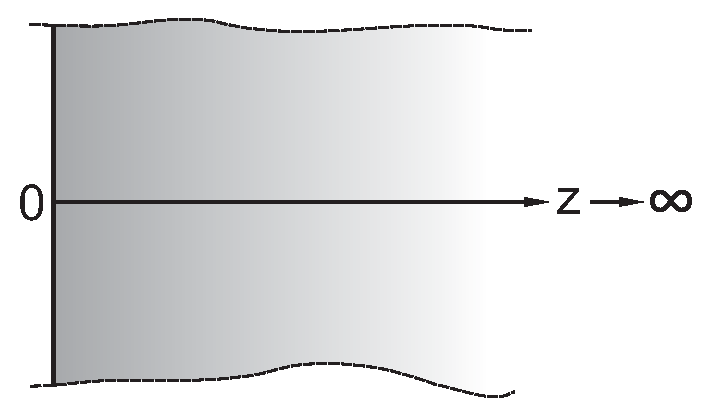
\includegraphics[width=0.5\textwidth]{T/figures/LHD.eps}
\caption{\label{figLHD}One side limited domain in cartesian coordinates.}
\end{figure}
%%%%%%%%%%%%%%%%%%%%%%%%%%%%%%%%%%%%%%%%%%%%%%%%%%%%%%%%%%%%%%%%%%%%%%%%%%%%%%%%%%%%%%%%
\subsection{Analytical solution}

The one dimensional heat transport in a domain limited just by one side can be derived by \eqref{eqn:lhd}
\begin{equation}
T(x,t) = T_0 \operatorname{erfc} \left(\frac{x}{\sqrt{4\alpha t}}\right),
\label{eqn:lhd}
\end{equation}
where $T_0$ is the initial temperature and $\alpha = \lambda/c\rho$ is the heat diffusivity coefficient of the used material.

%%%%%%%%%%%%%%%%%%%%%%%%%%%%%%%%%%%%%%%%%%%%%%%%%%%%%%%%%%%%%%%%%%%%%%%%%%%%%%%%%%%%%%%%
\subsection{Numerical solution}
\subsubsection{Model setup}

The numerical model consists of 60 line elements connected by 61 nodes along the z-axis (figure \ref{fig-ms-lhd}). The distances of the nodes $\Delta z$ is one meter. At $z=\unit[0]{m}$ there is a constant temperature boundary condition. 
\begin{figure}%[img-msldh]
%\label{img-msldh}
\centering
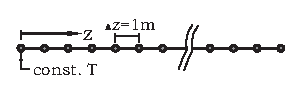
\includegraphics[width=0.5\textwidth]{T/figures/ms-lhd.eps}
\caption{\label{fig-ms-lhd}Spatial discretisation of the numerical model.}
\end{figure}
%%%%%%%%%%%%%%%%%%%%%%%%%%%%%%%%%%%%%%%%%%%%%%%%%%%%%%%%%%%%%%%%%%%%%%%%%%%%%%%%%%%%%%%%%%%%%%%%%%%%
\subsubsection{Parameters}

The material properties for this model setup are given in Tab.~\ref{tab-ldhp}.
%\begin{table}[tab-ldhp]
%\centering
%\label{tab-ldhp}
%\caption{Material properties}
%\begin{tabular}{|c|l|l|}
%\hline
%symbol & quantity & value \\
%\hline
%$\rho$   & density of the solid & 2500  kg$\cdot$m$^{-3}$ \\			
%\hline
%$c$	     & thermal capacity	    & 1000  J$\cdot$kg$^{-1}\cdot$K$^{-1}$ \\
%\hline
%$\lambda$ & thermal conductivity	& 3.2  W$\cdot$m$^{-1}\cdot$K$^{-1}$ \\
%\hline
%\end{tabular}
%\end{table}
\begin{table}[h]%[tab-ldhp]
\caption{\label{tab-ldhp}Material properties.}
\begin{center}
\begin{tabular}{ll}
\toprule
parameter & value \\
\midrule
density $\rho$ of the solid & 2500  kg$\cdot$m$^{-3}$ \\			
heat capacity	$c$	    & 1000  J$\cdot$kg$^{-1}\cdot$K$^{-1}$ \\
thermal conductivity $\lambda$	& 3.2  W$\cdot$m$^{-1}\cdot$K$^{-1}$ \\
\bottomrule
\end{tabular}
\end{center}
\end{table}
Using these values, the outcome for the heat diffusivity constant $\alpha = \lambda/c\rho$ in \eqref{EqHT} is $\alpha=1.28\cdot$10$^{-6}m^2/s$.
%%%%%%%%%%%%%%%%%%%%%%%%%%%%%%%%%%%%%%%%%%%%%%%%%%%%%%%%%%%%%%%%%%%%%%%%%%%%%%%%%%%%%%%%%%%%%%%%%%%%%%%%
\subsubsection{Temporal discretisation}

The \textit{Neumann} stability criteria has to be restrained so that the temperature gradient can't be inverted by diffusive fluxes. Using \eqref{eqn:ne-ldh} the best time step can be estimated by
\begin{equation}
\operatorname{Ne} = \frac{\alpha\Delta t}{(\Delta z)^2}\leq\frac{1}{2}.
\label{eqn:ne-ldh}
\end{equation}
With $\Delta z=\unit[1]{m}$ and $\alpha=\unit[1.28 \cdot 10^{-6}]{m^2/s}$ the outcome for the timestep is $\Delta t\leq \unit[390.625]{s}$ or 4.5 days respectively.
%%%%%%%%%%%%%%%%%%%%%%%%%%%%%%%%%%%%%%%%%%%%%%%%%%%%%%%%%%%%%%%%%%%%%%%%%%%%%%%%%%%%%%%%
\subsection{Results}

%The following figure show the comparison of the solution of \eqref{eqn:lhd} and the numerical simulation results. Fig.~\ref{fig-lhd-all} shows the temperature distribution along the model domain after 2 months, 1 year, 2 years and 4 years.
The following figure (Fig.~\ref{fig-lhd-all}) show the comparison of the solution of \eqref{eqn:lhd} and the numerical simulation results. It is demontrated the temperature distribution along the model domain after 2 months, 1 year, 2 years and 4 years.
\begin{table}%[]
\caption{Benchmark deposit.}
\begin{center}
\begin{tabular}{lll}
\toprule
Deposit & Version & Date \\
\midrule
T$\backslash$TDiff$\backslash$TDiff & 4.7.03 & Jun.~2008 \\
\bottomrule
\end{tabular}
\end{center}
\end{table}
\begin{figure}%[img-lhd-all]
\centering
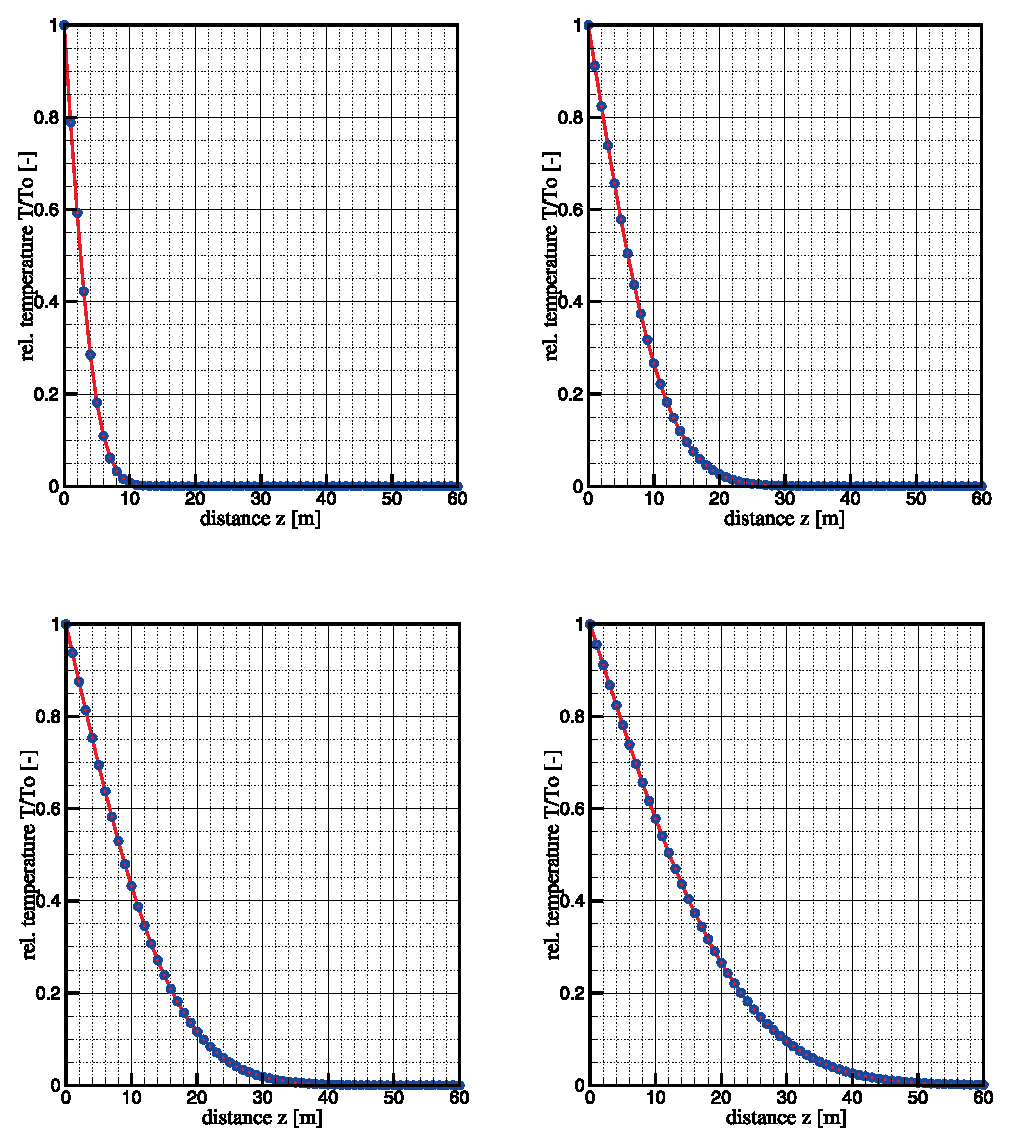
\includegraphics[width=0.9\textwidth]{T/figures/lhd-all.eps}
\caption{\label{fig-lhd-all}Temperature distribution along the z-axis after 2 months, 1 year, 2 years and 4 years (from top left to down right).}
\end{figure}
%\clearpage

%%%%%%%%%%%%%%%%%%%%%%%%%%%%%%%%%%%%%%%%%%%%%%%%%%%%%%%%%%%%%%%%%%%%%%%%%%%%%%%%%%%%%%%%%%
\section{Linear heat diffusion in a wall}

\subsection{Problem definition}

In the last example there was a domain limited only by one side with a constant temperature at the boundary. The following problem shows the profile of a homogeneous and isotropic wall with a constant heat flow $Q_A$ on the left and a constant temperature $T_L$ on the right boundary (Fig.~\ref{fig-lhdw}). This example consists also just of diffusive heat transport.
\begin{figure}[h]
\centering
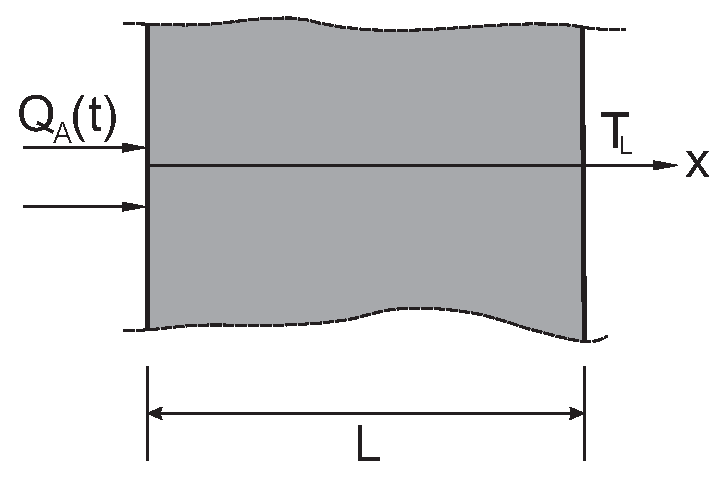
\includegraphics[width=0.5\textwidth]{T/figures/LHDW.eps}
\caption{\label{fig-lhdw}Heat conduction through a wall.}
\end{figure}
%%%%%%%%%%%%%%%%%%%%%%%%%%%%%%%%%%%%%%%%%%%%%%%%%%%%%%%%%%%%%%%%%%%%%%%%%%%%%%%%%%%%%%%%%%%%%%%%%%%%%%%%%%%%%%%%%%%%
\subsection{Analytical solution}

A solution for this problem can be found by solving the heat conduction equation \eqref{EqHT} using \textit{Fourier}'s method (see \cite{HaeSamVoi:92}). It can be shown:
\begin{equation}
\begin{split}
	T(x,t) & = T_L+\frac{Q_A}{\lambda}(L-x) + \sum_{n=1}^{\infty} \\ & - \frac{8L}{(2n-1)^2\pi^2}\;\frac{Q_A}{\lambda} \cos{\frac{(2n-1)\pi x}{2L}}\;e^{(-\frac{(2n-1)^2\pi^2}{4L^2}\alpha\,t)}
	\label{eqn:lhdw}
\end{split}
\end{equation}
with $T_L$ is the initial temperature, $Q_A$ is the constant heat source, $\lambda$ is the thermal conductivity and $\alpha$ is the heat diffusivity constant.

%%%%%%%%%%%%%%%%%%%%%%%%%%%%%%%%%%%%%%%%%%%%%%%%%%%%%%%%%%%%%%%%%%%%%%%%%%%%%%%%%%%%%%%%%%%%%%%%%%%%%%%%%%%%%%%%%%%%%%
\subsection{Numerical solution}
\subsubsection{Model setup}

The numerical model consits of 40 line elements and 41 nodes along the x-axis (Fig.~\ref{fig-mslhdw}). The step size $\Delta z$ is set to $\unit[0.1]{m}$. On the left boundary a constant source term is set. The right side obtaines a constant temperature.
\begin{figure}%[htbp]
\centering
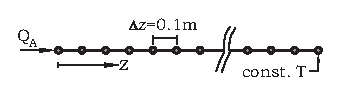
\includegraphics[width=0.5\textwidth]{T/figures/ms-lhdw.eps}
\caption{\label{fig-mslhdw}Boundary conditions and discretisation for the numerical model.}
\end{figure}

\subsubsection{Parameters}

Tab.~\ref{tab-ldhwp} shows the values of the used material properties. The heat diffusivity constant $\alpha$ 
outcomes to $\alpha = \unit[3.1 \cdot 10 ^{-6}]{m^{2}}$/s. 
\begin{table}[h]
\caption{\label{tab-ldhwp}Material properties.}
\begin{center}
\begin{tabular}{ll}
\toprule
parameter 						& value \\
\midrule
heat source $Q_A$ 				& $\unit[30]{W \cdot m^{-2}}$ \\			
initial temperatur $T_L$		& $\unit[25]{^{\circ}C}$ \\
wall thickness $L$				& $\unit[4]{m}$ \\
density of the solid $\rho$ 	& $\unit[2000]{kg \cdot m^{-3}}$ \\			
thermal capacity	$c$  		& $\unit[900]{J \cdot kg^{-1} \cdot K^{-1}}$ \\
thermal conductivity $\lambda$	& $\unit[5.5]{W \cdot m^{-1} \cdot K^{-1}}$ \\
\bottomrule
\end{tabular}
\end{center}
\end{table}

%%%%%%%%%%%%%%%%%%%%%%%%%%%%%%%%%%%%%%%%%%%%%%%%%%%%%%%%%%%%%%%%%%%%%%%%%%%%%%%%%%%%%%%%%%%%%%%%%%%%%%%%%%%%%%%%%%%%%%%
\subsection{Results}

The comparison of analytical and numerical solution is presented in Fig.~\ref{fig-lhdw-all}. The figure shows the distribution of the temperatue along the profile of the wall. Due to the thickness of the wall, the heat transport takes very long, after 5.000.000 seconds ($\approx$ 58 days) the temperature distribution becomes staedy-state.
\begin{figure}[h]
\centering
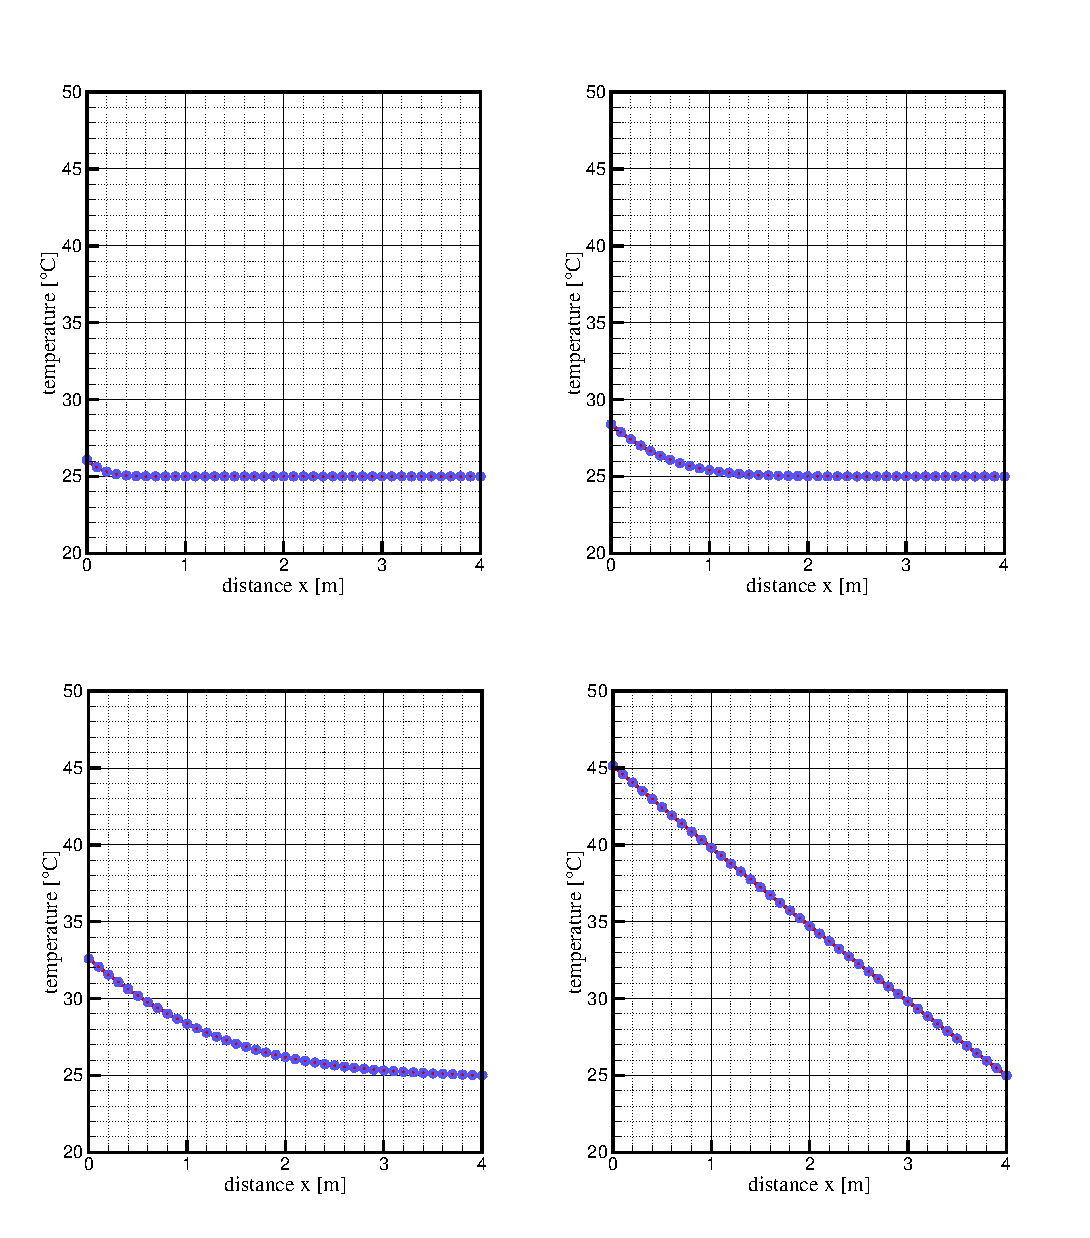
\includegraphics[width=0.8\textwidth]{T/figures/lhdw-all.eps}
\caption{Temperature distribution along the wall profile after 10.000, 100.000, 500.000 and 5.000.000 seconds (from top left to down right).}
\label{fig-lhdw-all}
\end{figure}
\begin{table}
\caption{Benchmark deposit.}
\begin{center}
\begin{tabular}{lll}
\toprule
Deposit & Version & Date \\
\midrule
T$\backslash$TDiff-wall$\backslash$TDiff-wall & 4.7.03 & Jun.~2008 \\
\bottomrule
\end{tabular}
\end{center}
\end{table}
%\clearpage

%%%%%%%%%%%%%%%%%%%%%%%%%%%%%%%%%%%%%%%%%%%%%%%%%%%%%%%%%%%%%%%%%%%%%%%%%%%%%%%%%%%%%%%%%%

\section{Radial heat diffusion}

\subsection{Problem definition}

A slice with a hole in its centre, that means a 2D annulus, which consists of a solid of a constant temperature is exposed to a higher temperature at the surface of its hole. The aim of this calculation is to simulate the heat transfer through this homogeneous solid by the use of an axisymmetric model. Fig.~\ref{figT1} shows a sketch of the calculation area
\begin{figure}%[htbp]
\centering
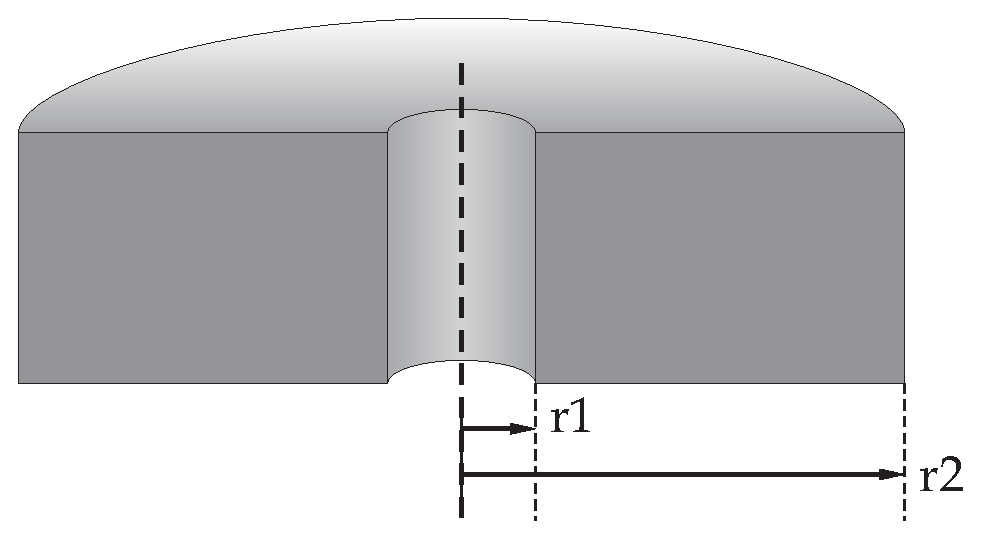
\includegraphics[width=0.5\textwidth]{T/figures/radial-heat-transport.eps}
\caption{\label{figT1}Calculation area.}
\end{figure}
assuming a homogeneous solid, a constant temperature in the whole body at the beginning and a heating of the slice at the inner surface of the hole .
%\textsl{Assumptions}
%
%\begin{tabbing}
%\=xxxxxxxxxxxxx  \=xxxxxxxxxxxxxxxxxxxxxxx \kill
%\> Temperature: \> constant temperature in the whole body at the beginning, \\
%\>  \> heating of the slice at the inner surface of the hole \\[0.5ex]
%\> Solid:		    \> homogeneous
%\end{tabbing}

\subsection{Model set-up of the 1D numerical model}

The inner radius $R_1$ of the axisymmetric model is $\unit[1]{m}$ and the outer radius $R_2$ is $\unit[5]{m}$. The numerical model consists of 40 elements and 41 nodes. The initial temperature in the whole area is $\unit[25]{^{\circ}C}$. At the right boundary of the numerical model a thermal boundary condition is set with a constant value of $\unit[25]{^{\circ}C}$. At the left boundary a source term for heat flux of $q=\unit[30]{W/m^2}$ is defined. Thereby the continuous heating of the solid is simulated. The used parameters of the solid are listed in Tab.~\ref{tab11}. The simulation of 5000 time steps with a constant time step length of $\unit[1000]{s}$ is done.
\begin{table}[h]
\caption{\label{tab11}Material properties.}
\begin{center}
\begin{tabular}{ll}
\toprule
parameter 						& value \\
\midrule
density of the solid $\rho$ 	& $\unit[2.0]{t \cdot m^{-3}}$ \\			
thermal capacity $c$		    & $\unit[900]{J \cdot kg^{-1} \cdot K^{-1}}$ \\
thermal conductivity $\lambda$	& $\unit[5.5]{W \cdot m^{-1} \cdot K^{-1}}$ \\
\bottomrule
\end{tabular}
\end{center}
\end{table}

\subsection{Evaluation method}

For the heating of the annulus with the inner radius $R_1$ and the outer radius $R_2$ the following analytical solution for temperature in dependency on the radius $r$ was used
\begin{equation}
T(r) = \frac{R_1 q}{\kappa}\ln\left(\frac{R_2}{r}\right) + T_0.
\label{eq11}
\end{equation}
Here $q$ represents the heat source, $\lambda$ the thermal conductivity and $T_0$ the initial temperature.
%{\small
%with
%\begin{itemize}
%\item[$q$] -- heat source (W/m$^2$)
%\item[$\lambda$] -- thermal conductivity (W/(m$\cdot$K))
%\item[$T_0$] -- initial temperature ($^{\circ}$C)
%\end{itemize}
%}

\subsection{Results}

The results of the analytical equation for the temperature distribution over the model length are compared to those of the numerical simulation by GeoSys/RockFlow. Fig.~\ref{figT2} shows the temperature distribution over the radius of the annulus. Obviously, with the axisymmetric model a GeoSys/RockFlow simulation generates comprehensible results that agree well with the analytic solution.
\begin{figure}[htbp]
\centering
\includegraphics[width=0.75\textwidth]{T/figures/figT2.eps}
\caption{\label{figT2}Temperature distribution over the radius}
\end{figure}

\begin{table}[h]
\caption{Benchmark deposit}
\begin{center}
\begin{tabular}{lll}
\toprule
Deposit & Version & Date \\
\midrule
T$\backslash$heat1d$\backslash$T\_1D\_axi & 4.7.02 & Mar.~2008 \\
\bottomrule
\end{tabular}
\end{center}
\end{table}
%\clearpage



%%%%%%%%%%%%%%%%%%%%%%%%%%%%%%%%%%%%%%%%%%%%%%%%%%%%%%%%%%%%%%%%%%%%%%%%%%%%%%%%%%%%%%%%%%

\section{Temperature-dependent thermal properties}

For temperature \underline{and} pressure depending thermal properties see chapter \ref{chap-FP} "Fluid property functions".

%%%%%%%%%%%%%%%%%%%%%%%%%%%%%%%%%%%%%%%%%%%%%%%%%%%%%%%%%%%%%%%%%%%%%%%%%%%%%%%%%%%%%%%%%%

\section{Heat transport in a fracture}

\subsection{Problem definition}

This problem shows 1D heat transport by advection and diffusion in a $\unit[100]{m}$ long fracture. The fracture is fully saturated with groundwater, flowing with constant velocity. There is no rock matrix around the fracture which could store heat. Fig.~\ref{fig-addiff1} give a view about the situation.
\begin{figure}[h]
\centering
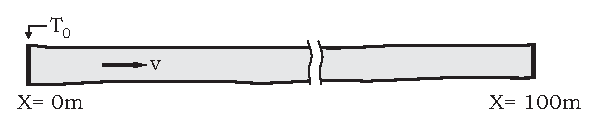
\includegraphics[width=0.5\textwidth]{T/figures/Ad-Diff-Problem-def.eps}
\caption{\label{fig-addiff1}A fully saturated fracture with flowing groundwater and a constant temperature at the left border.}
\end{figure}

%%%%%%%%%%%%%%%%%%%%%%%%%%%%%%%%%%%%%%%%%%%%%%%%%%%%%%%%%%%%%%%%%%%%%%%%%%%%%%%%%%%%%%%%%%%%%%%%%%%%%%%%%%%%%%%%%%%%
\subsection{Parameters}

The fracture is described as a porous medium with $\unit[100]{\%}$ porosity, so that no solid material influences the heat transport process. The properties of the fluid are in Tab.~\ref{tab-addiff}.
\begin{table}[h]
\caption{\label{tab-addiff}Material properties.}
\begin{center}
\begin{tabular}{ll}
\toprule
parameter 						& value \\
\midrule
density $\rho$ 					& $\unit[1000]{kg \cdot m^{-3}}$ \\			
thermal capacity $c$			& $\unit[4000]{J \cdot kg^{-1} \cdot K^{-1}}$ \\
thermal conductivity $\lambda$ 	& $\unit[0.6]{W \cdot m^{-1} \cdot K^{-1}}$ \\
\bottomrule
\end{tabular}
\end{center}
\end{table}
These values cause a diffusivity constant for water of $\alpha=\unit[1.5 \cdot 10^{-7}]{m^2/s}$. The groundwater velocity in the fracture is $v=\unit[3.0 \cdot 10^{-7}]{m^2/s}$.

%%%%%%%%%%%%%%%%%%%%%%%%%%%%%%%%%%%%%%%%%%%%%%%%%%%%%%%%%%%%%%%%%%%%%%%%%%%%%%%%%%%%%%%%%%%%%%%%%%%%%%%%%%%%%%%%%%%%%%
\subsection{Analytical solution}

For 1D-advective/diffusive transport, an analytical solution is given by \textsc{Ogata $\&$ Banks} as
\begin{equation}
T(x,t)=\frac{T_0}{2}\bigg( \operatorname{erfc} \frac{x-v_x\cdot t}{\sqrt{4\alpha t}} + e^{\frac{v_x\cdot x}{\alpha}} \operatorname{erfc}\frac{x+v_x\cdot t}{\sqrt{4\alpha t}}\bigg),
\label{eqn:addiff1}
\end{equation}
where $T_0$ is the constant temperature at $x=0$, $v$ is the groundwater velocity and $\alpha$ is the heat diffusivity coefficient of water (see \cite{HaeSamVoi:92},\cite{Kol:97}).

%%%%%%%%%%%%%%%%%%%%%%%%%%%%%%%%%%%%%%%%%%%%%%%%%%%%%%%%%%%%%%%%%%%%%%%%%%%%%%%%%%%%%%%%%%%%%%%%%%%%%%%%%%%%%%%%%%%%%%%
\subsection{Numerical solution}

The mesh for the numerical model consists of 501 nodes combining 500 line elements. The distance between the nodes is $\Delta x=\unit[0.2]{m}$.

\paragraph{Boundary conditions}
\begin{itemize}
	\item Left border:
	\begin{compactitem}
		\item constant source term (liquid flow) with $Q=\unit[3.0 \cdot 10^{-7}]{m^3/s}$
		\item constant temperature with $T=\unit[1]{^\circ C}$
	\end{compactitem}
	\item Right border:	
	\begin{compactitem}
		\item constant pressure with $P=\unit[100,000]{kPa}$
	\end{compactitem}
	\item Initial conditions:
	\begin{compactitem}
		\item pressure with $P=\unit[100,000.0]{kPa}$ for whole domain
		\item temperature $T=\unit[0]{^\circ C}$ for whole domain
	\end{compactitem}
	\item Time step:
	\begin{compactitem}
		\item $\Delta t=\unit[133,333.0]{s}$
	\end{compactitem}
\end{itemize}
With the given parameters, the \textsc{Neumann} criteria \eqref{eqn:ne-ldh} results on $\operatorname{Ne}=0.5$ which guarantees the numerical stability of the diffusion part of the transport process. The \textit{Courant} criteria, given by
\begin{equation}
	C=\frac{v_x\cdot\Delta t}{\Delta x}\leq1
	\label{eqn:addiff2}
\end{equation}\\
results to $C=0.2$.
%%%%%%%%%%%%%%%%%%%%%%%%%%%%%%%%%%%%%%%%%%%%%%%%%%%%%%%%%%%%%%%%%%%%%%%%%%%%%%%%%%%%%%%%%%%%%%%%%%%%%%%%%%%%%%%%%%%%%%%
\subsection{Results}

In Fig.~\ref{fig-addiff-re1} the comparison of analytical and numerical solution is plotted. The figure shows the temperature breakthrough curve at the end of the fracture at $x=\unit[100]{m}$. The numerical results show an acceptable agreement to the analytical solution. In a further step, the diffusion part of the heat transport process was avoided by minimizing the thermal conductivity of the fluid. Fig.~\ref{fig-addiff-re2} shows the breakthrough curve for only advective heat transport.
\begin{table}[h]
\caption{Benchmark deposit}
\begin{center}
\begin{tabular}{lll}
\toprule
Deposit & Version & Date \\
\midrule
T$\backslash$Ogata-Banks$\backslash$Ogata-Banks & 4.7.03 & Jul.~2008 \\
\bottomrule
\end{tabular}
\end{center}
\end{table}
\begin{figure}[H]
\centering
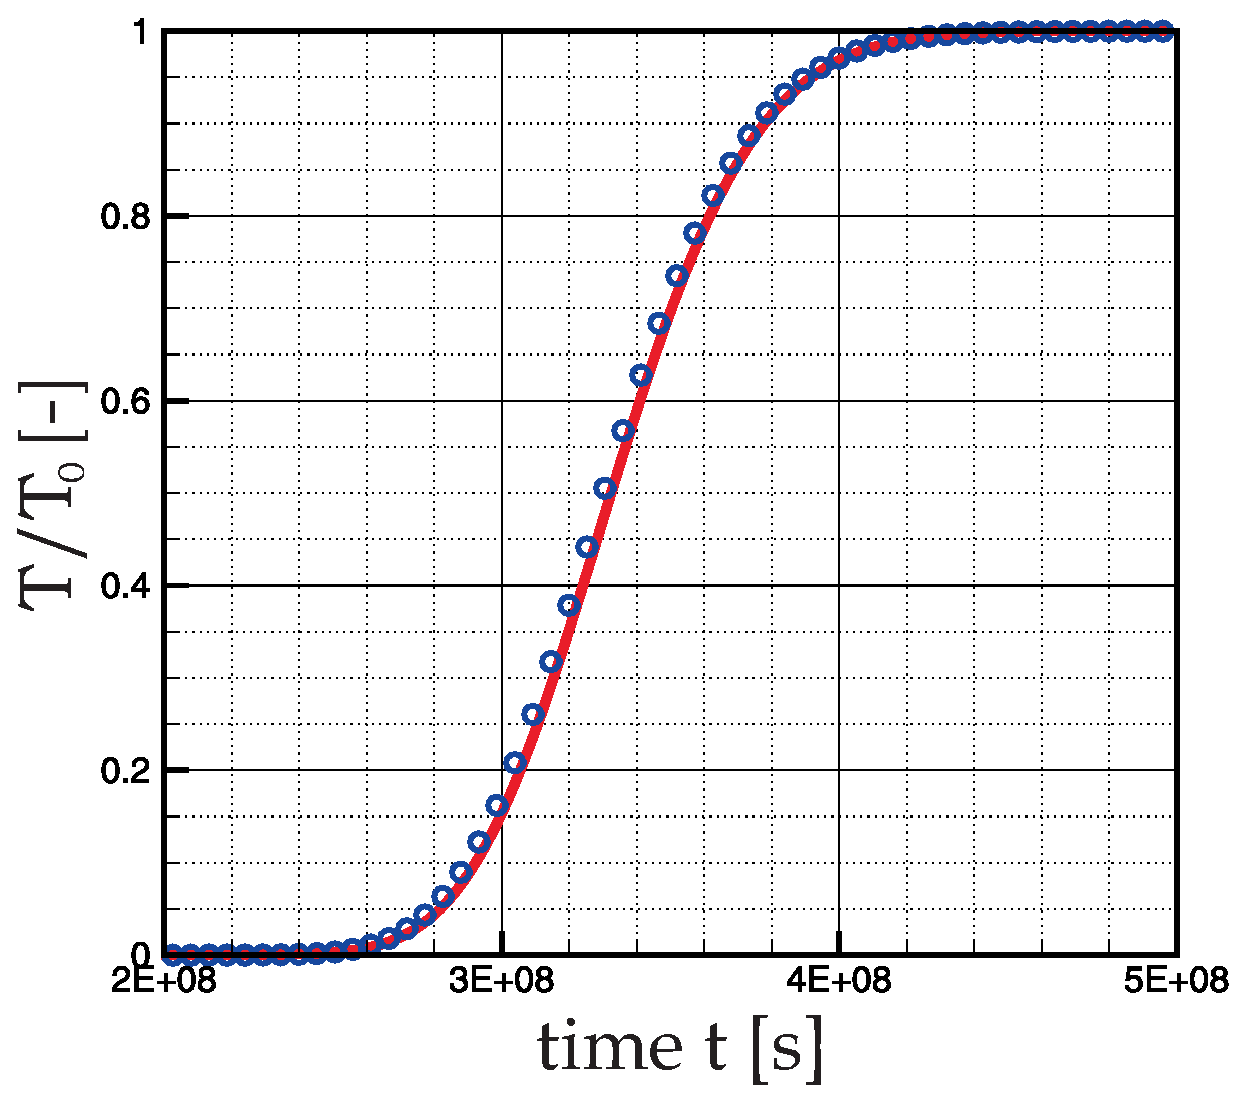
\includegraphics[width=0.5\textwidth]{T/figures/Ad-Diff.eps}
\caption{\label{fig-addiff-re1}Temperature breakthrough curve at the point $x=\unit[100]{m}$.}
\end{figure}
\begin{figure}[h]
\centering
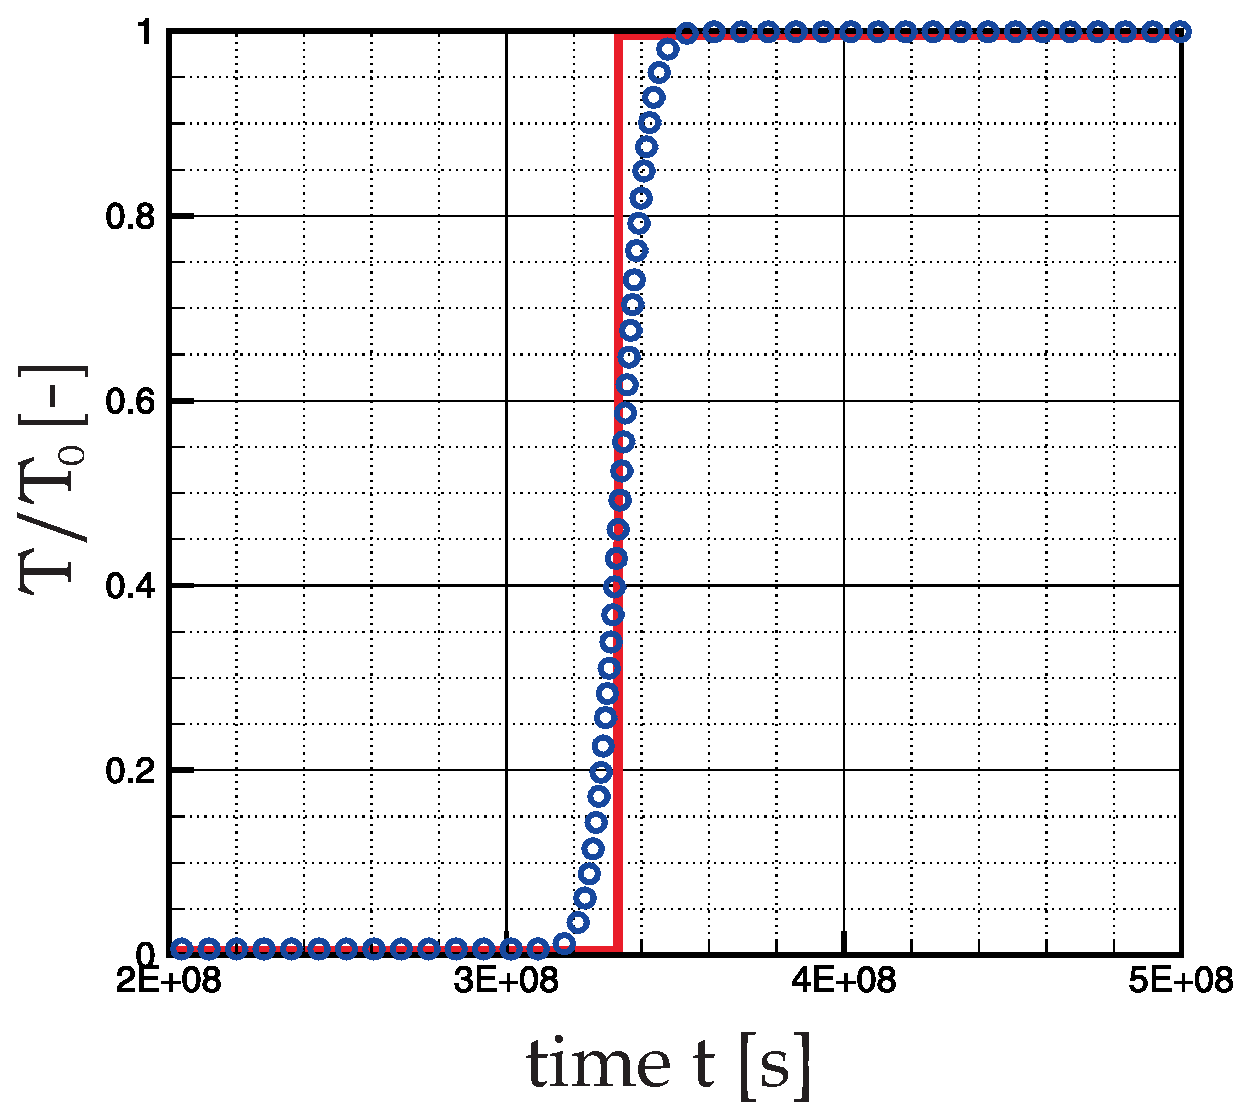
\includegraphics[width=0.5\textwidth]{T/figures/advection.eps}
\caption{\label{fig-addiff-re2}Temperature breakthrough curve when diffusion is avoided.}
\end{figure}
%\clearpage

%%%%%%%%%%%%%%%%%%%%%%%%%%%%%%%%%%%%%%%%%%%%%%%%%%%%%%%%%%%%%%%%%%%%%%%%%%%%%%%%%%%%%%%%%%

\section{Heat transport in fracture-matrix systems}

\subsection{Problem definition}

Based on the last benchmark example, the heat transport by advection and diffusion in a fracture, this problem is extended by heat diffusion through a rock matrix orthogonal to the fracture (Fig.~\ref{fig-lauwerier-problem}). 
\begin{figure}[h]
\centering
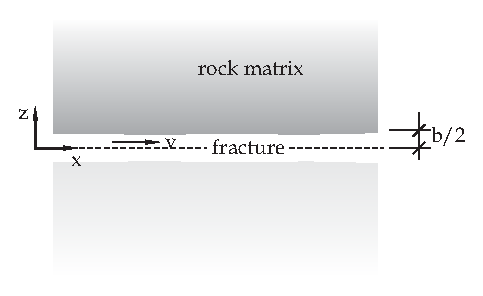
\includegraphics[width=0.5\textwidth]{T/figures/lauwerier-problem.eps}
\caption{\label{fig-lauwerier-problem}Heat transport in a fracture-matrix system.}
\end{figure}
%%%%%%%%%%%%%%%%%%%%%%%%%%%%%%%%%%%%%%%%%%%%%%%%%%%%%%%%%%%%%%%%%%%%%%%%%%%%%%%%%%%%%%%%%%%%%%%%%%%%%%%%%%%%%%%%%%%%
\subsection{Analytical solution}

For this problem an analytical solution is given by \textsc{Lauwerier} (1955) (see \cite{Kol:97}) with following restrictions:
\begin{compactitem}
\item in the fracture, heat is transported just by advection,
\item in the rock matrix, heat transport takes place by diffusion (only along the z-axis).
\end{compactitem}
The \textsc{Lauwerier} equation is given by
\begin{equation}
T_D=\begin{cases}
0, & t_D < x_D \\
\operatorname{erfc}\left\{ \frac{\beta}{\sqrt{\alpha\left(t_D-x_d\right)}} \left[ x_D+\frac{1}{2\beta}\left( z_D-\frac{1}{2} \right) \right]\right\}, & t_D > x_D
\end{cases},   z_D \geq\frac{1}{2}
\label{lauwerier}
\end{equation}
with the following dimensionless parameters:
\begin{equation}
t_D=\frac{v_x}{b}t,\ \ \ x_D=\frac{x}{b},\ \ \ z_D=\frac{z}{b},\ \ \ \alpha =\frac{\lambda ^{r}}{c^{r}\rho ^{r}}\frac{1}{bv_x},\ \ \ \beta = \frac{\lambda^{r}}{c^{w}\rho^{w}}\frac{1}{bv_x}
\end{equation}
where $b$ is the fracture width, $\lambda$ is the thermal conductivity, $c$ is the heat capacity, $\rho$ is the density and $r$ and $w$ are rock or water material parameters respectively.

\subsection{Model setup}

The \textsc{Lauwerier}-problem is formed as a coupling of advective 1D heat transport in x-direction and diffusive 1D heat transport in z-direction. This means, that nodes in the rock matrix are not influenced by their left or right neighbors. The matrix elements are connected to the fracture elements orthogonaly. Fig.~\ref{fig-lauwerier-grid} shows a schematical description of the model setup. Because of the symmetry, the numerical model calculates just the domain above the x-axis. 
\begin{figure}[h]
\centering
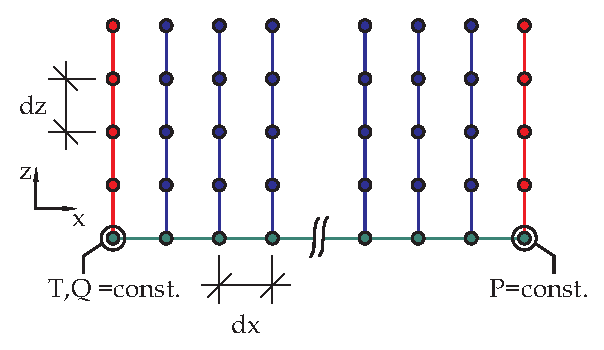
\includegraphics[width=0.65\textwidth]{T/figures/lauwerier-grid.eps}
\caption{\label{fig-lauwerier-grid}Alignment of the grid for the numerical model.}
\end{figure}
Fig.~\ref{fig-lauwerier-scheme} shows the positions of observation points which were chosen to evaluate the numerical model by the comparison with analytical solutions. 
\begin{figure}[h]
\centering
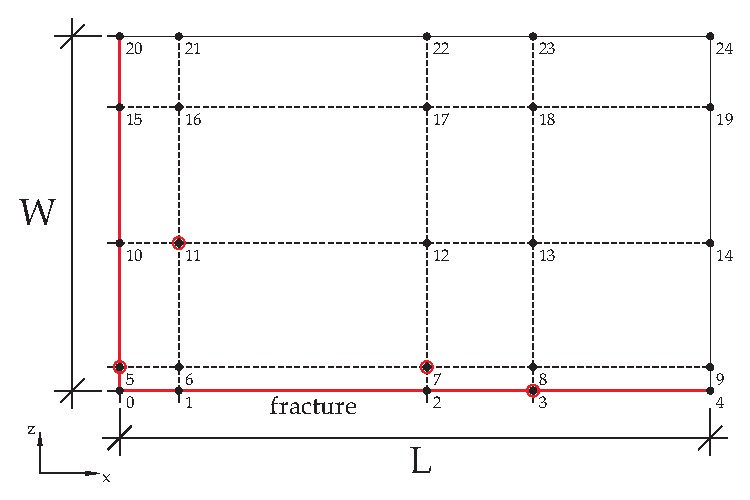
\includegraphics[width=0.65\textwidth]{T/figures/lauwerier-scheme.eps}
\caption{\label{fig-lauwerier-scheme}Positions of observation points for temperature breakthrough curves.}
\end{figure}

\subsection{Parameters}

The chosen parameters and material properties for this solution are shown in Tab.~\ref{tab-lauwerier-parameters}.
\begin{table}[ht]
\caption{\label{tab-lauwerier-parameters}Model parameters for the \textsc{Lauwerier}-problem.}
\begin{center}
\begin{tabular}{llll}
\toprule
parameter 						& value \\
\midrule
\multicolumn{2}{c}{\textit{spatial discretisation}} \\
fracture length $L$				& $\unit[50]{m}$  \\
matrix width $W$ 				& $\unit[63.25]{m}$  \\
step size X $\Delta x$ 			& $\unit[2]{m}$  \\
step size Z $\Delta z$ 			& $\unit[0.1265]{m}$  \\
half of fracture width $b/2$ 	& $\unit[1.0 \cdot 10^{-3}]{m}$  \\
groundwater velocity $v_x$ 		& $\unit[1.0 \cdot 10^{-4}]{m/s}$ \\
\cmidrule{1-4}
\multicolumn{2}{c}{\textit{temporal discretisation}}\\
timesteps $\Delta t$ 			& $\unit[2.0 \cdot 10^{5}]{s}$  \\ 
No. of timesteps 				& 2500 \\
total time 						& $\unit[5.0 \cdot 10^{8}]{s}$  \\
\cmidrule{1-4}
\multicolumn{2}{c}{\textit{material properties -- solid}}\\
thermal conductivity $\lambda$ 	& $\unit[1]{W \cdot m^{-1} \cdot K^{-1}}$  \\
heat capacity $c$ 				& $\unit[1000]{J \cdot kg^{-1} \cdot K^{-1}}$  \\
density $\rho$ 					& $\unit[2500]{kg \cdot m^{-3}}$  \\
\cmidrule{1-4}
\multicolumn{2}{c}{\textit{material properties -- fluid}}\\
heat capacity $c$ 				& $\unit[4000]{J \cdot kg^{-1} \cdot K^{-1}}$  \\
density $\rho$ 					& $\unit[1000]{kg \cdot m^{-3}}$  \\
\bottomrule
\end{tabular}
\end{center}
\end{table}

\subsection{Results}

The quality of the numerical results can be shown by temperature distribution curves for several times in the rock matrix. Fig.~\ref{fig-lauwerier-rock} shows the temperature profiles for $x=\unit[0]{m}$ at three moments $t'$. The numerical solution has a very good agreement to the analytical results. Temperature profiles along the fracture at $z=\unit[0]{m}$ are plotted in Fig.~\ref{fig-lauwerier-fracture}. For long simulation times ( $t'=1000; t'=600$) both solutions fits very well together. For short simulation times, the numerical solution differ slightly from the analytical results. This discrapancy for short simulation times can be examined in Fig.~\ref{fig-lauwerier-points}, where temperature breakthrough cures for certain points (see Fig.~\ref{fig-lauwerier-scheme}) is plotted.
\begin{table}[h]
\caption{Benchmark deposit.}
\begin{center}
\begin{tabular}{lll}
\toprule
Deposit & Version & Date \\
\midrule
T$\backslash$Lauwerier$\backslash$Lauwerier & 4.7.03 & Jul.~2008 \\
\bottomrule
\end{tabular}
\end{center}
\end{table}
\begin{figure}[H]
\centering
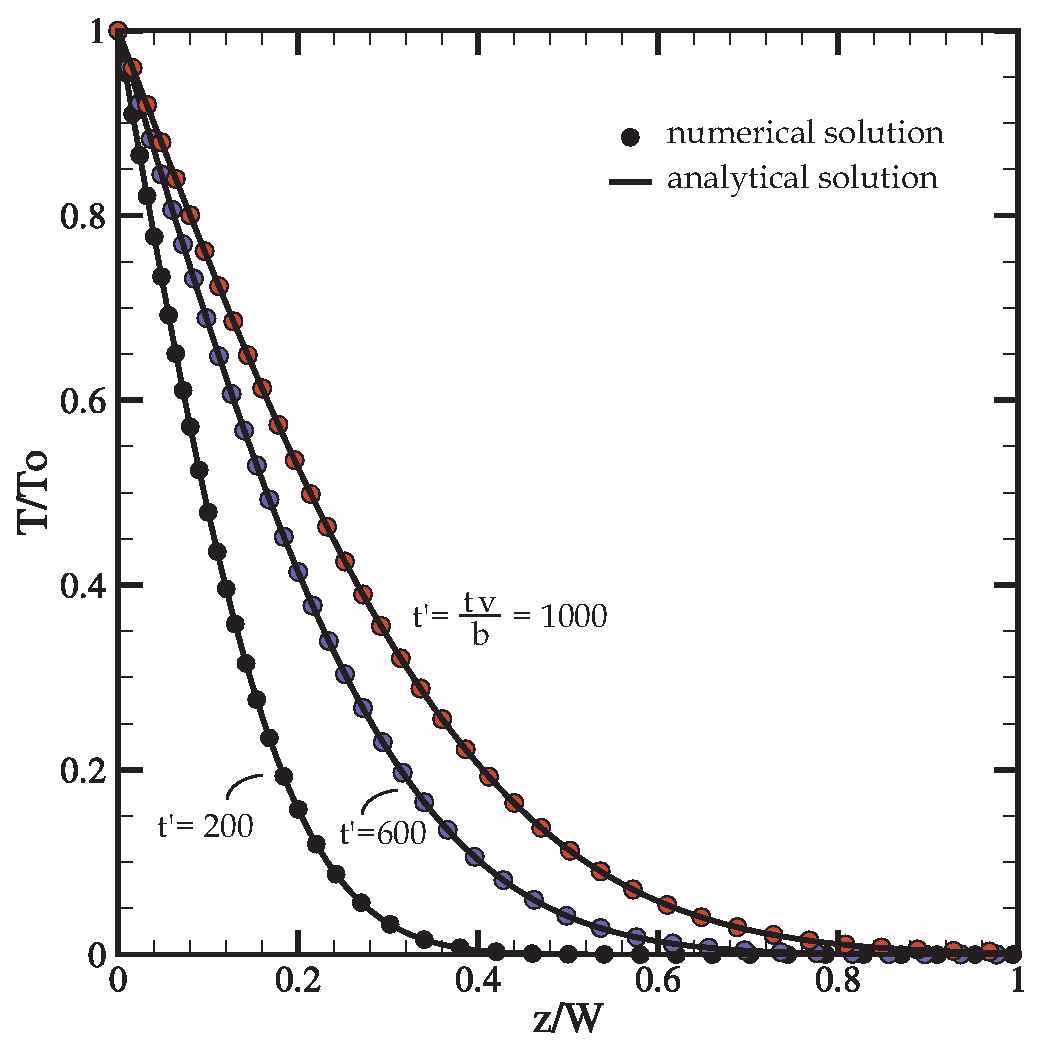
\includegraphics[width=0.6\textwidth]{T/figures/lauwerier-rock.eps}
\caption{Temperature distribution orthogonal to the fracture at $x=0$ at three different times.}
\label{fig-lauwerier-rock}
\end{figure}
\begin{figure}[H]
\centering
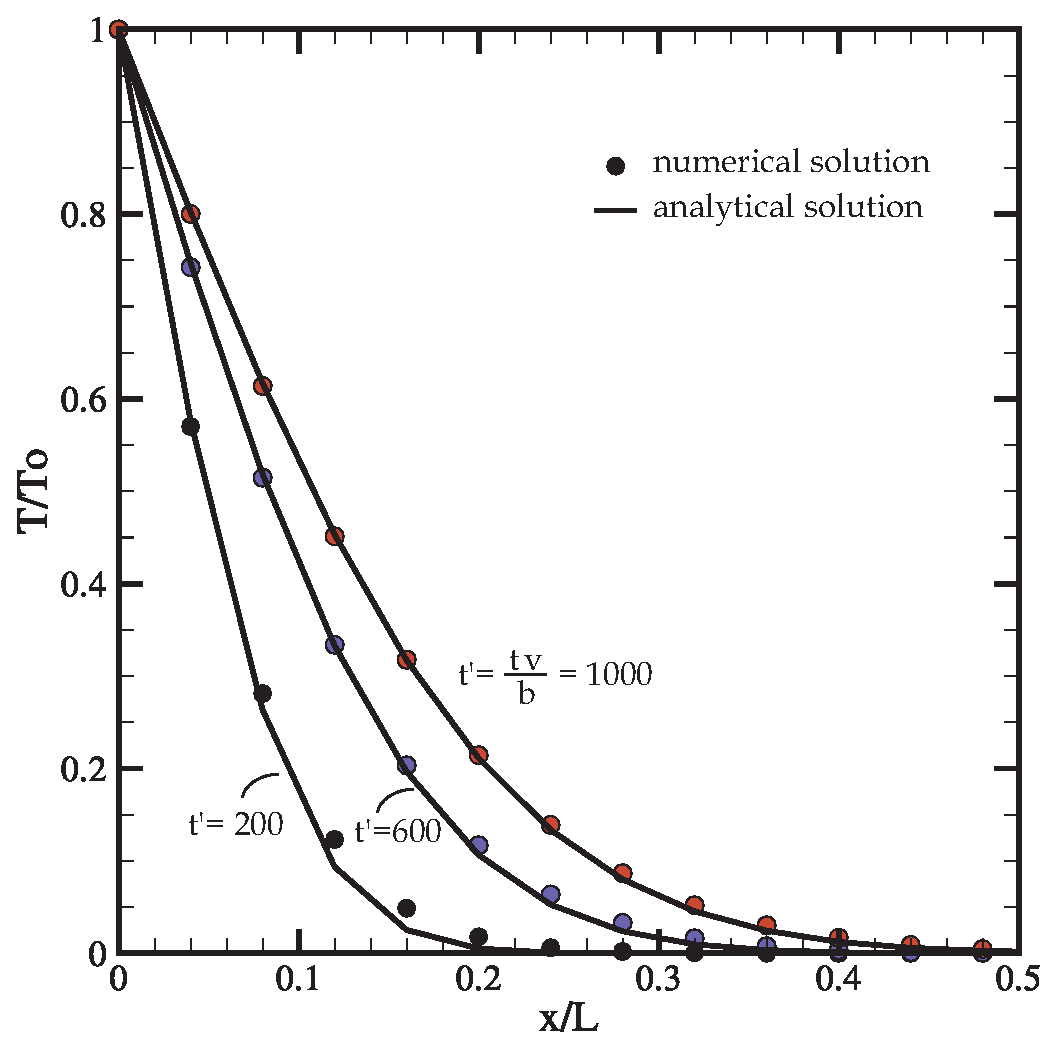
\includegraphics[width=0.6\textwidth]{T/figures/lauwerier-fracture.eps}
\caption{Temperature distribution along the fracture at three different times.}
\label{fig-lauwerier-fracture}
\end{figure}
\begin{figure}[H]
\centering
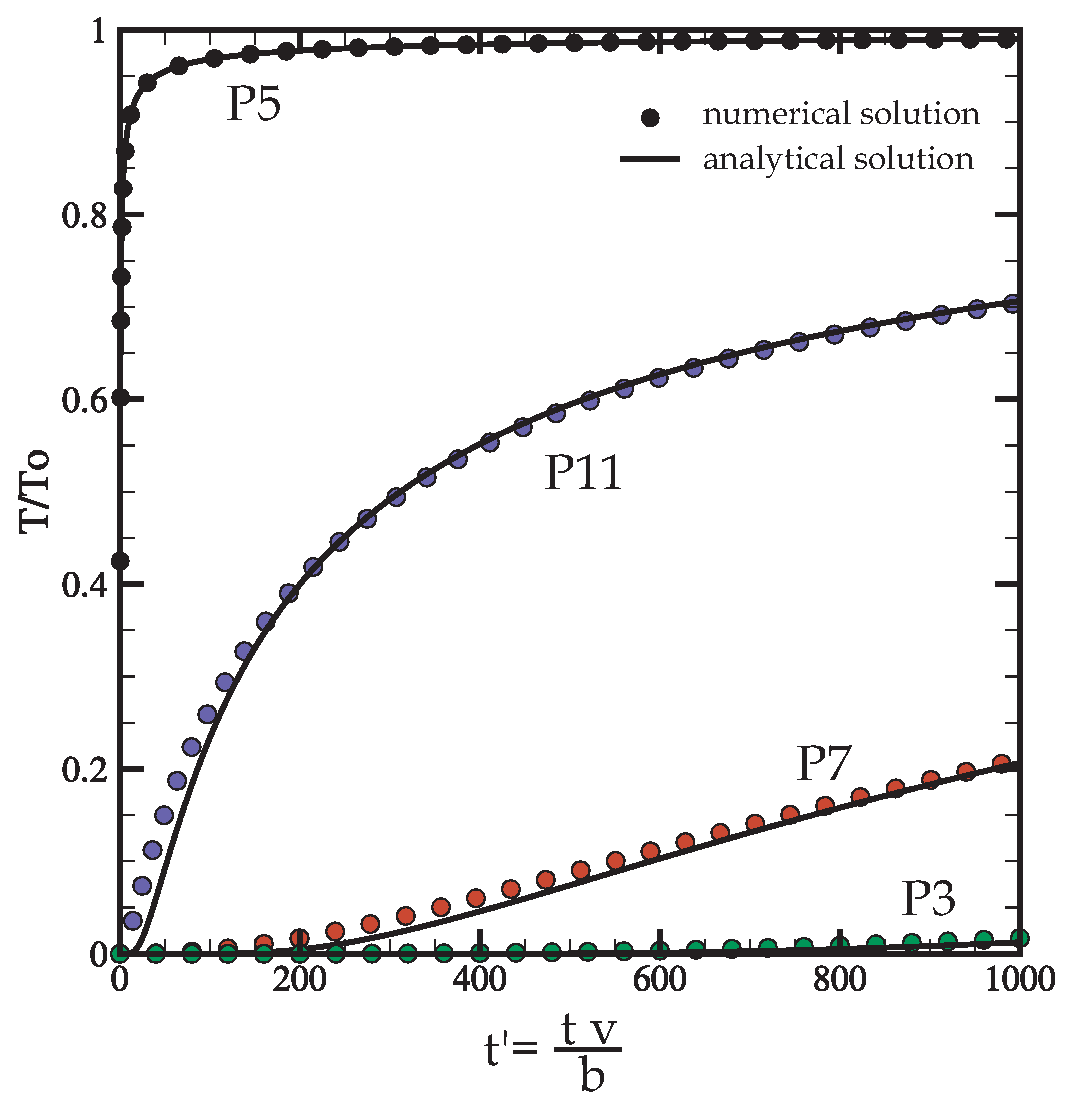
\includegraphics[width=0.6\textwidth]{T/figures/lauwerier-points.eps}
\caption{Temperature breakthrough curves at certain points in the rock matrix.}
\label{fig-lauwerier-points}
\end{figure}
%\clearpage

%%%%%%%%%%%%%%%%%%%%%%%%%%%%%%%%%%%%%%%%%%%%%%%%%%%%%%%%%%%%%%%%%%%%%%%%%%%%%%%%%%%%%%%%%%

\section{Heat transport in fracture-matrix systems: 3D case study}

\subsection{Problem Definition}

The following problem deals with simulating fluid flow and heat transport in a 3 dimensional heterogeneous faulted geological system.  
%figure1
\label{sec:model}
\begin{figure}[htbp]
    \begin{center}
        \includegraphics[width=0.40\textwidth]{T/figures/2u2f_fig1.eps}
        \caption{Sample model consisting of two geological layers cut by a system of two crossing faults.}
        \label{fig1}
    \end{center}
\end{figure}

The model volume consists of two sub-horizontal geological layers, including two dipping faults (Figure \ref{fig1}). The horizontal north-south and east-west extensions are 200 m, resulting in a horizontal model area of 40,000 m$^{2}$. The two geological layers are vertically bordered by three curved surfaces. The elevation of top, middle and bottom surface is 55 m $\pm{}$ 5m, 0 m $\pm{}$ 7 m and -45 m $\pm{}$ 5 m, respectively.  Therefore, an average thickness of 55 m for layer 1 and 45 m for layer 2 is established (Table \ref{tab:geometry}).

%table1
\begin{table}[htbp]
    \begin{center}
        \caption{Geometrical attributes of the geological layers and faults.}
        \begin{tabular}{lccc}
          \hline
          property & unit & layer1 & layer2\\
          \hline
          \hline
          average thickness $t$ & [m] & 55 & 45\\
          \hline
                   &      & fault1 & fault2\\
          \hline
          \hline
          dip direction & [$^\circ$] & 316.7 & 225\\
          dip & [$^\circ$] & 80.6 & 63.2\\
          length $l$ & [m] & 233.5 & 183.8\\
          \hline        
        \end{tabular}
        \label{tab:geometry}
    \end{center}
\end{table}

Both faults are penetrating the two geological layers. Fault 1 has a length of 233 m and is striking North-East, with dip coordinates of 316.7$^\circ{}$; 80.6$^\circ{}$. Fault 2 has a length of 184 m and  is oriented perpendicular to fault 1, having dip coordinates of 225$^\circ{}$; 63.2$^\circ{}$ (Table \ref{tab:geometry}).

\subsection{Initial and boundary conditions}
%figure2
\begin{figure}[htbp]
    \begin{center}
        \includegraphics[width=0.48\textwidth]{T/figures/2u2f_fig2.eps}
        \caption{Pressure boundary condition of the sample model.}
        \label{fig2}
    \end{center}
\end{figure}
During the simulation, a general flow field from the South to the North is generated. Dirichlet (or first-type) boundary conditions for pressure are set along the southern and northern boundaries (Figure\ref{fig2}). According to the definition of hydrostatic pressure, the pressure at the southern border is constant at p(x, y = -100 m, z) = $\rho{}$gz + 1.75$\cdot10^{6}$ Pa and at the northern border at p(x, y = 100 m, z) = $\rho{}$gz + 1.25 $\cdot10^{6}$ Pa (Figure \ref{fig2}), where $\rho{}$ [1000 kg/m$^{3}$], g [9.81 m/s$^{2}$] and z denotes the fluid density, gravitational acceleration and height of liquid column, respectively. An average hydraulic gradient $\nabla{}$h = 5$\cdot10^{5}$ Pa / 200 m = 0.25 from the South to the North is provided. For the remaining domain, a pressure value of 1.75$\cdot10^{6}$ Pa is initialized. 
%figure 3
\begin{figure}[htbp]
    \begin{center}
        \includegraphics[width=0.48\textwidth]{T/figures/2u2f_fig3.eps}
        \caption{Temperature boundary conditions of the sample model.} 
        \label{fig3}
    \end{center}
\end{figure}

To generate an inflow of hot and cold water from the southern border, Dirichlet boundary conditions for temperature are applied too (Figure \ref{fig3}). Along the southern border, temperature increases from 40$^\circ{}$C to 80$^\circ{}$C, in going from West to the East resulting in a temperature profile of T (x, y = -100 m, z) = 0.2$^\circ{}$C/m * x + 60$^\circ{}$C (Figure \ref{fig3}). For the remaining domain, the initial temperature is set to 60$^\circ{}$C.

\subsection{Parameters}

Table \ref{tab:layers} shows the hydraulic properties of the two geological layers.
%table2
\begin{table}[htbp]
    \begin{center}
        \caption{Porous medium properties of geological layers.}
        \begin{tabular}{lccc}
          \hline
          property & unit & layer1 & layer2\\
          \hline
          \hline
          porosity $\phi{}$ & [-] & 0.15 & 0.08\\
          storage $\beta{}$ & [1/Pa] & 7$\cdot10^{-10}$ & 7$\cdot10^{-10}$\\
          permeability $k$ & [m$^{2}$] & 2$\cdot10^{-14}$ & $10^{-14}$\\
          \hline
        \end{tabular}
        \label{tab:layers}
    \end{center}
\end{table}

To assure a variation of the hydraulic properties, the upper geological layer was modeled twice as conductive as the lower layer. The permeability $k$ of layer 1 is set to 2$\cdot10^{-14}$ m$^{2}$ and the porosity  $\phi{}$ to 0.15. For layer 2 the permeability k is set to $10^{-14}$ m$^{2}$ and the porosity $\phi{}$ to 0.08. The storage of both layers is derived from the bulk compressibility $\beta{}$ [1/Pa] of the rock and the embedded fluid. Assuming fissured rocks, the storage is set to 7$\cdot10^{-10}$ 1/Pa.

In table \ref{tab:faults} the relevant parameters for the system of the two faults are listed.
%table3
\begin{table}[htbp]
    \begin{center}
        \caption{Medium properties of faults.}
        \begin{tabular}{lccc}
          \hline
          property & unit & fault1 & fault2\\
          \hline
          \hline
          aperture $a$ & [m] & .05 & .05\\
          porosity $\phi{}$ & [-] & 1 & 1\\
          storage $\beta{}$ & [1/Pa] & 4.6$\cdot10^{-10}$ & 4.6$\cdot10^{-10}$\\
          permeability $k$ & [m$^2$] & $10^{-8}$ & 5$\cdot10^{-9}$\\
          \hline
        \end{tabular}
        \label{tab:faults}
    \end{center}
\end{table}

The permeability of fault 1 is set to $10^{-8}$ m$^{}$ and that of fault 2 to 5$\cdot10^{-9}$ m$^{2}$. The fault transmissivity is defined as the product of the fault permeability $k$ and aperture $a$. To ensure a high contrast between fault transmissivity and matrix conductivity, the aperture of both faults is set to 0.05 m. To provide free fluid flow in the faults, a porosity value of 1.0 is chosen. The storage in the faults is due to the fluid compressibility only and $\beta{}$  = 4.6$\cdot10^{-10}$ 1/Pa is assigned.

The simulation time is set to 145 years in order to observe in the simulation the major changes characterizing the temperature field. 

\subsection{Results}
\label{sec:results}

After approximately one month a steady state for pressure and velocity field is achieved (Figure \ref{fig4}).
%figure4
\begin{figure}[htbp]
    \begin{center}
        \begin{minipage}{0.40\textwidth}
            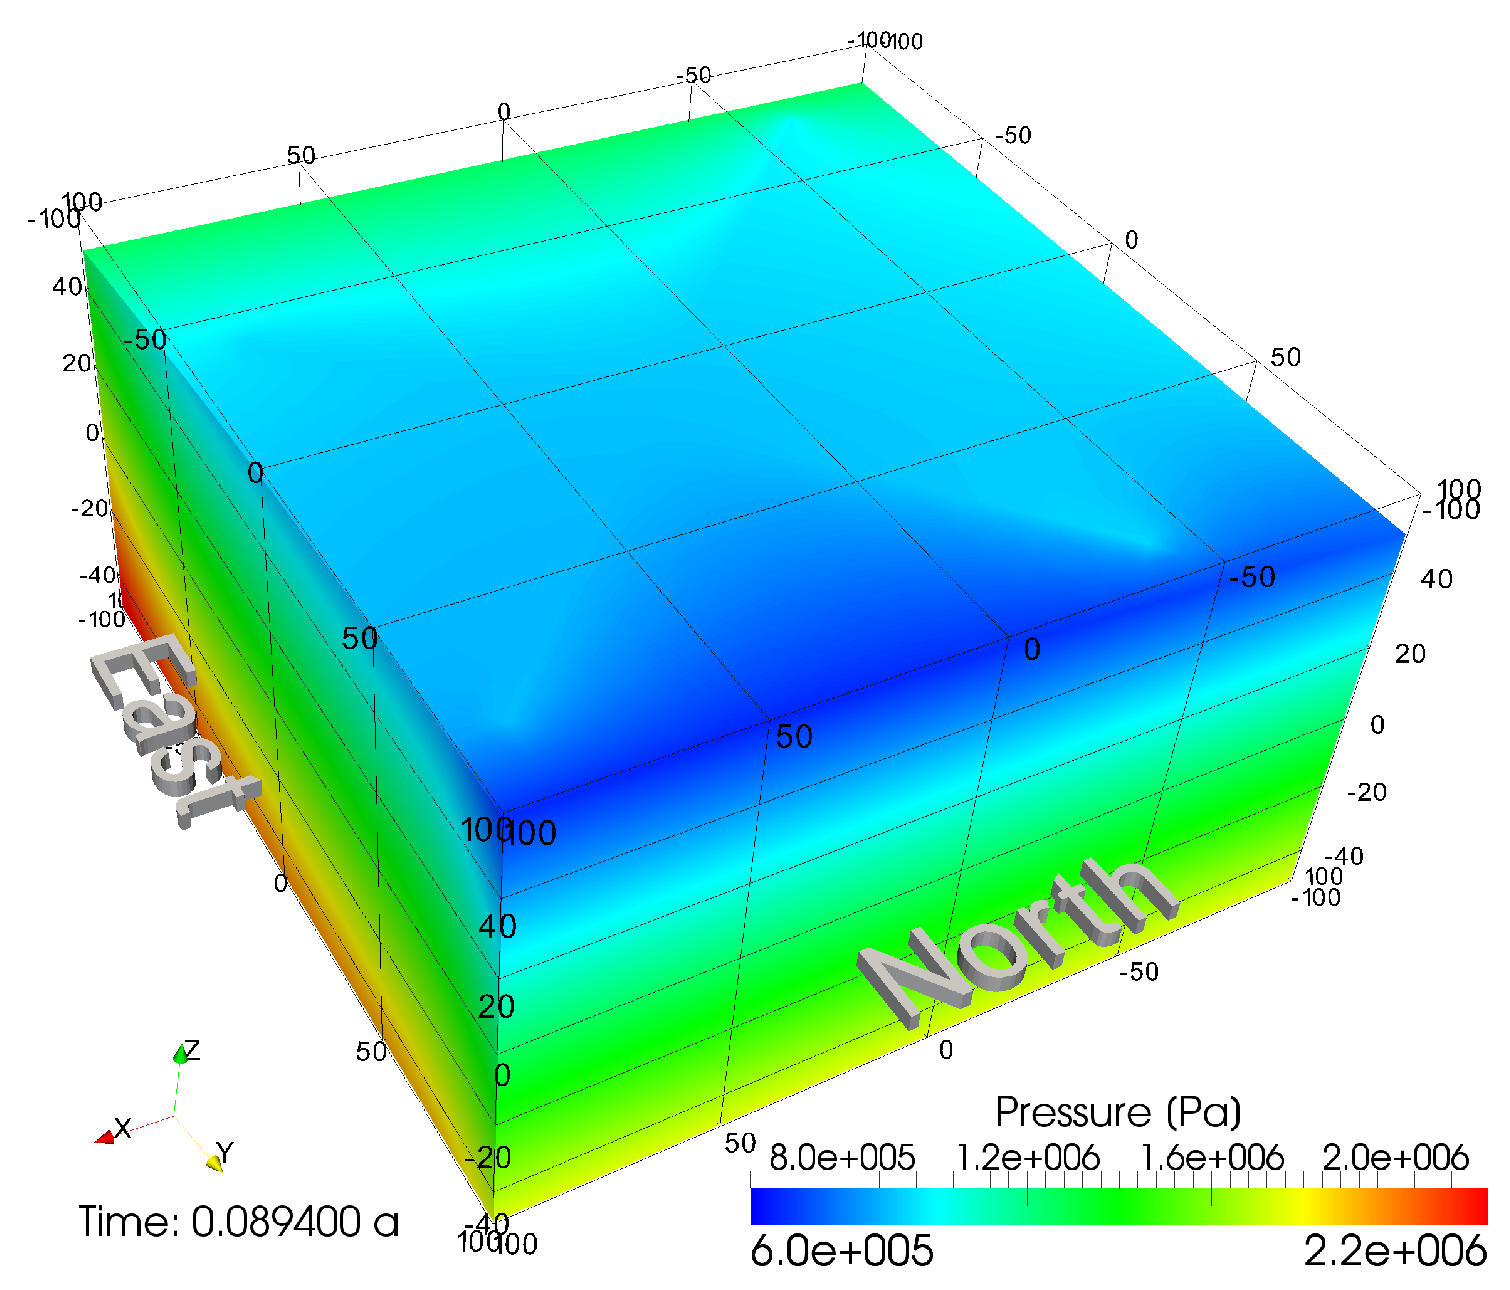
\includegraphics[width=1\textwidth]{T/figures/2u2f_fig4a.eps}
        \end{minipage}
        \begin{minipage}{0.40\textwidth}
            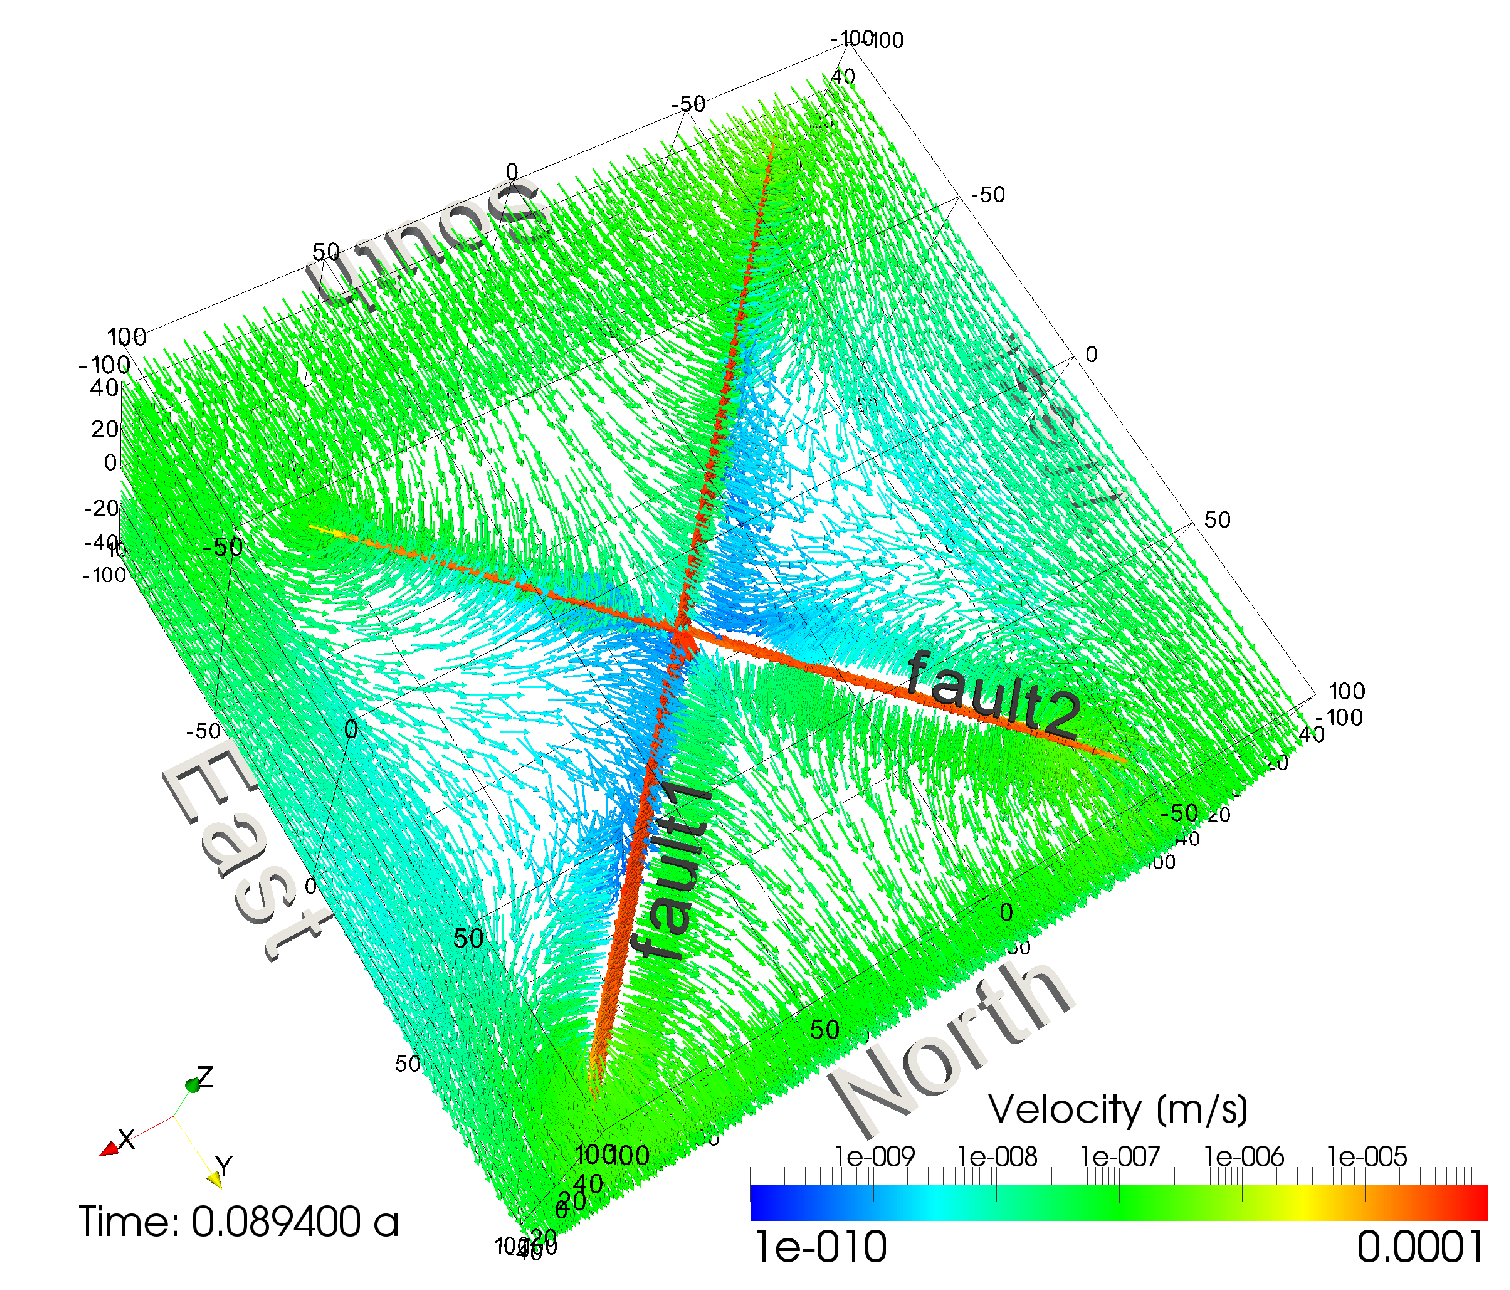
\includegraphics[width=1\textwidth]{T/figures/2u2f_fig4b.eps}
        \end{minipage}
        \caption{Simulated steady pressure (\ref{fig4}a) and velocity field (\ref{fig4}b) achieved after approx. 1 month.}
        \label{fig4}
    \end{center}
\end{figure}

Due to the fact that the implemented faults do not cut the southern and northern borders of the model, matrix flow is predominant in these areas. Accordingly, the highest pressure gradients are observed at the northern and southern borders of the model (Figure \ref{fig4}a). In proximity to the cutting faults, the isobars (surfaces of constant pressure) are sub-horizontal due to high flow rates within the faults. Maximum Darcy velocities of v = $\cdot10^{-4}$ m/s can be observed inside the faults (Figure \ref{fig4}b). Despite low pressure gradients, high flow rates occur in the fault planes. High values of fluid velocity are the result of the relative high transmissivity of the faults with respects to the surrounding domain.

Figure \ref{fig4}b shows the stationary flow field. As described above, highest flow velocities can be observed in the fault planes. The applied pressure boundary conditions force a regional flow field from the South to the North. The average velocity at the southern and northern regions is $10^{-7}$ m/s, with maximum inflow to the faults from the South. In the rest of the domain, outflow from the faults into the rock matrix is pronounced. In the central part of the model, faults act as the predominant flow paths. In contrast, low velocities (less than $10^{-8}$ m/s) characterize the eastern and western boundaries. An additional important fact is that at the southern edge of fault 1 and fault 2, backward flow from the North to the South occurs. Pressure equalisation within the faults results in higher matrix pressure at this area. This causes drainage of the rock matrix by the fault system.

Figure \ref{fig5}a-\ref{fig5}d shows the 45$^\circ{}$C, 55$^\circ{}$C, 65$^\circ{}$C and 75$^\circ{}$C contours at four different time stages.

%figure5
\begin{figure}[htbp]
    \begin{center}
        \begin{minipage}{0.35\textwidth}
            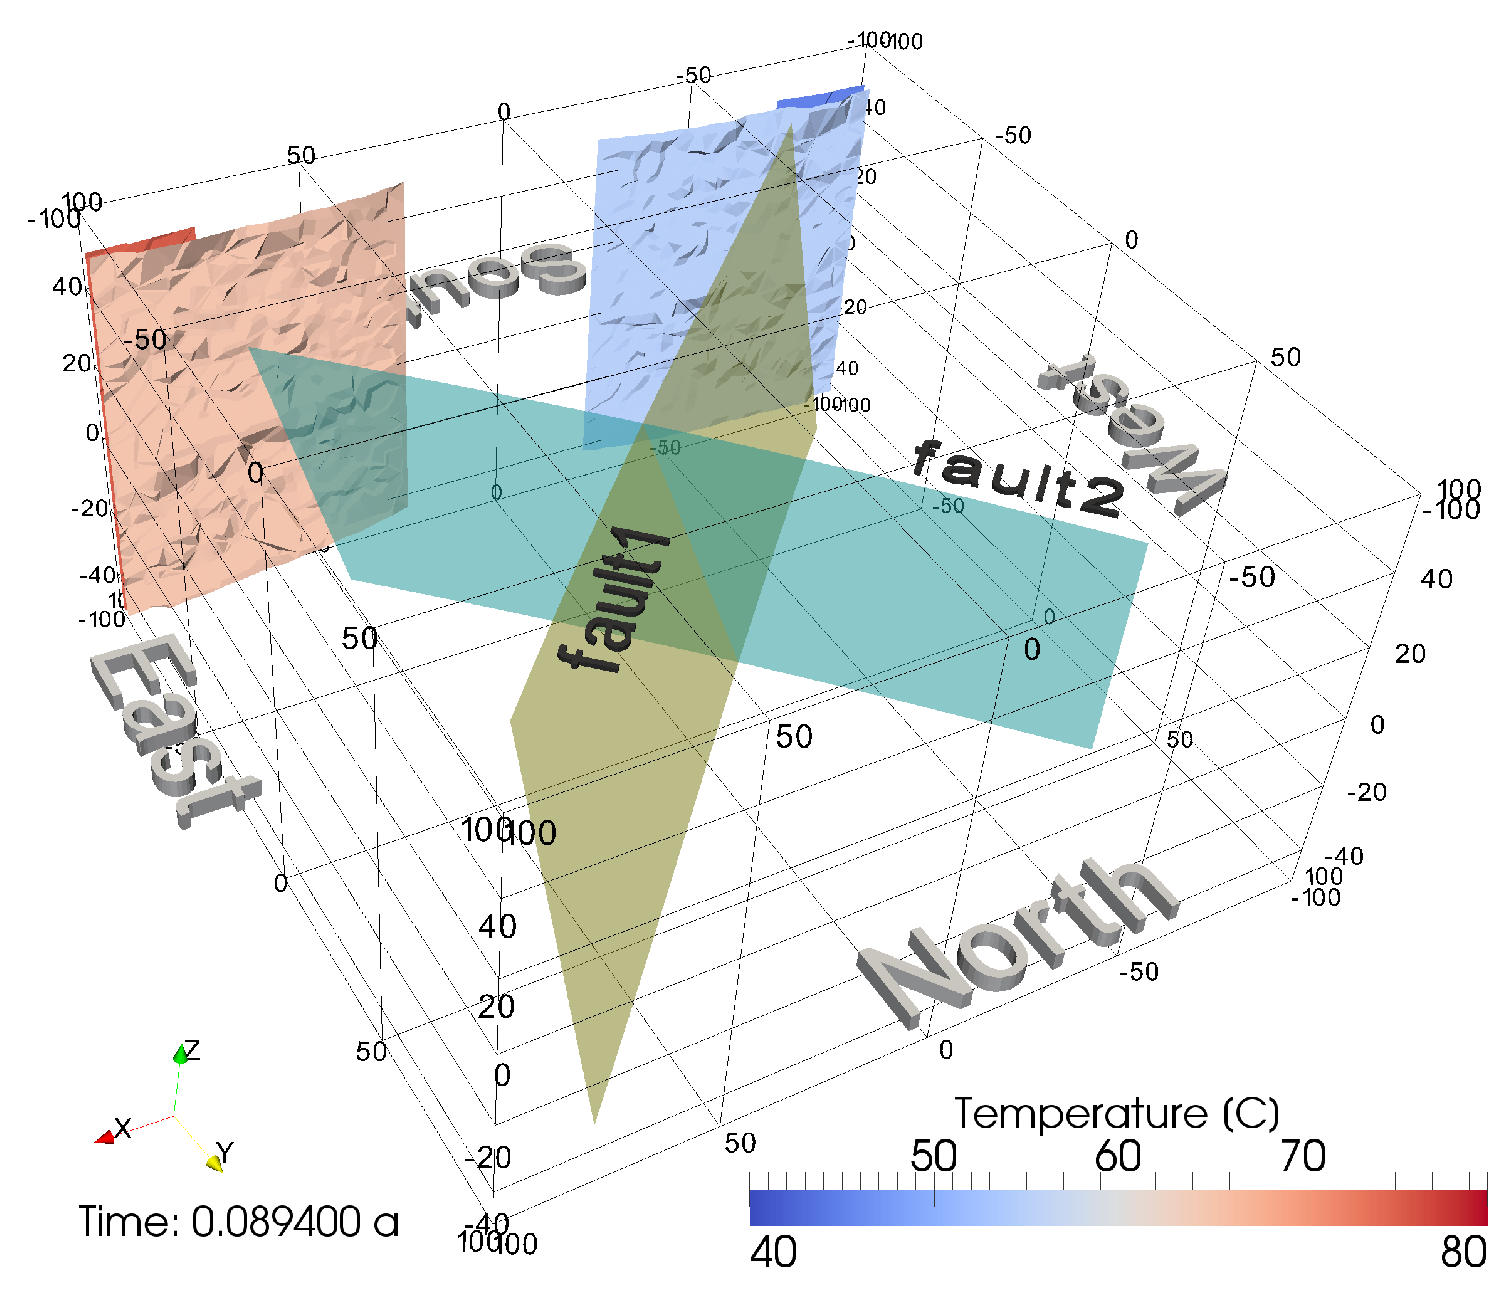
\includegraphics[width=1\textwidth]{T/figures/2u2f_fig5a.eps}
        \end{minipage}
        \begin{minipage}{0.35\textwidth}
            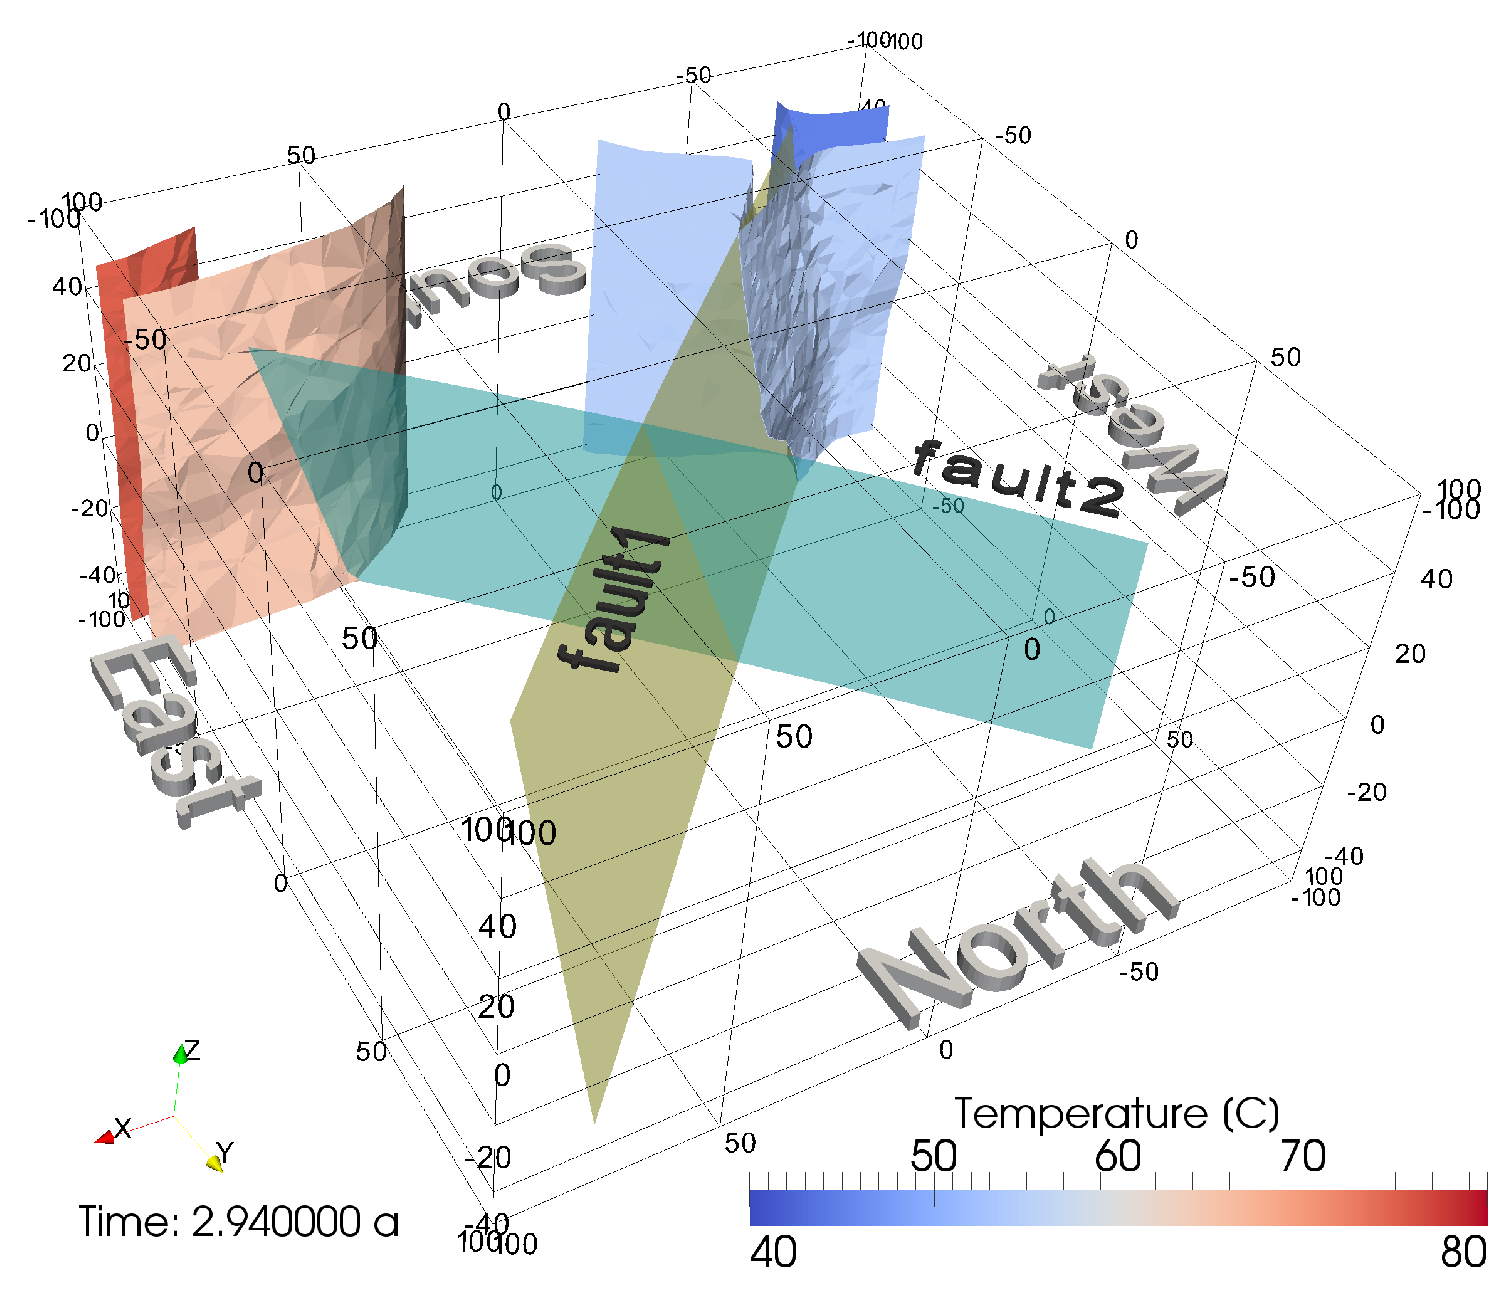
\includegraphics[width=1\textwidth]{T/figures/2u2f_fig5b.eps}
        \end{minipage}
        \begin{minipage}{0.35\textwidth}
            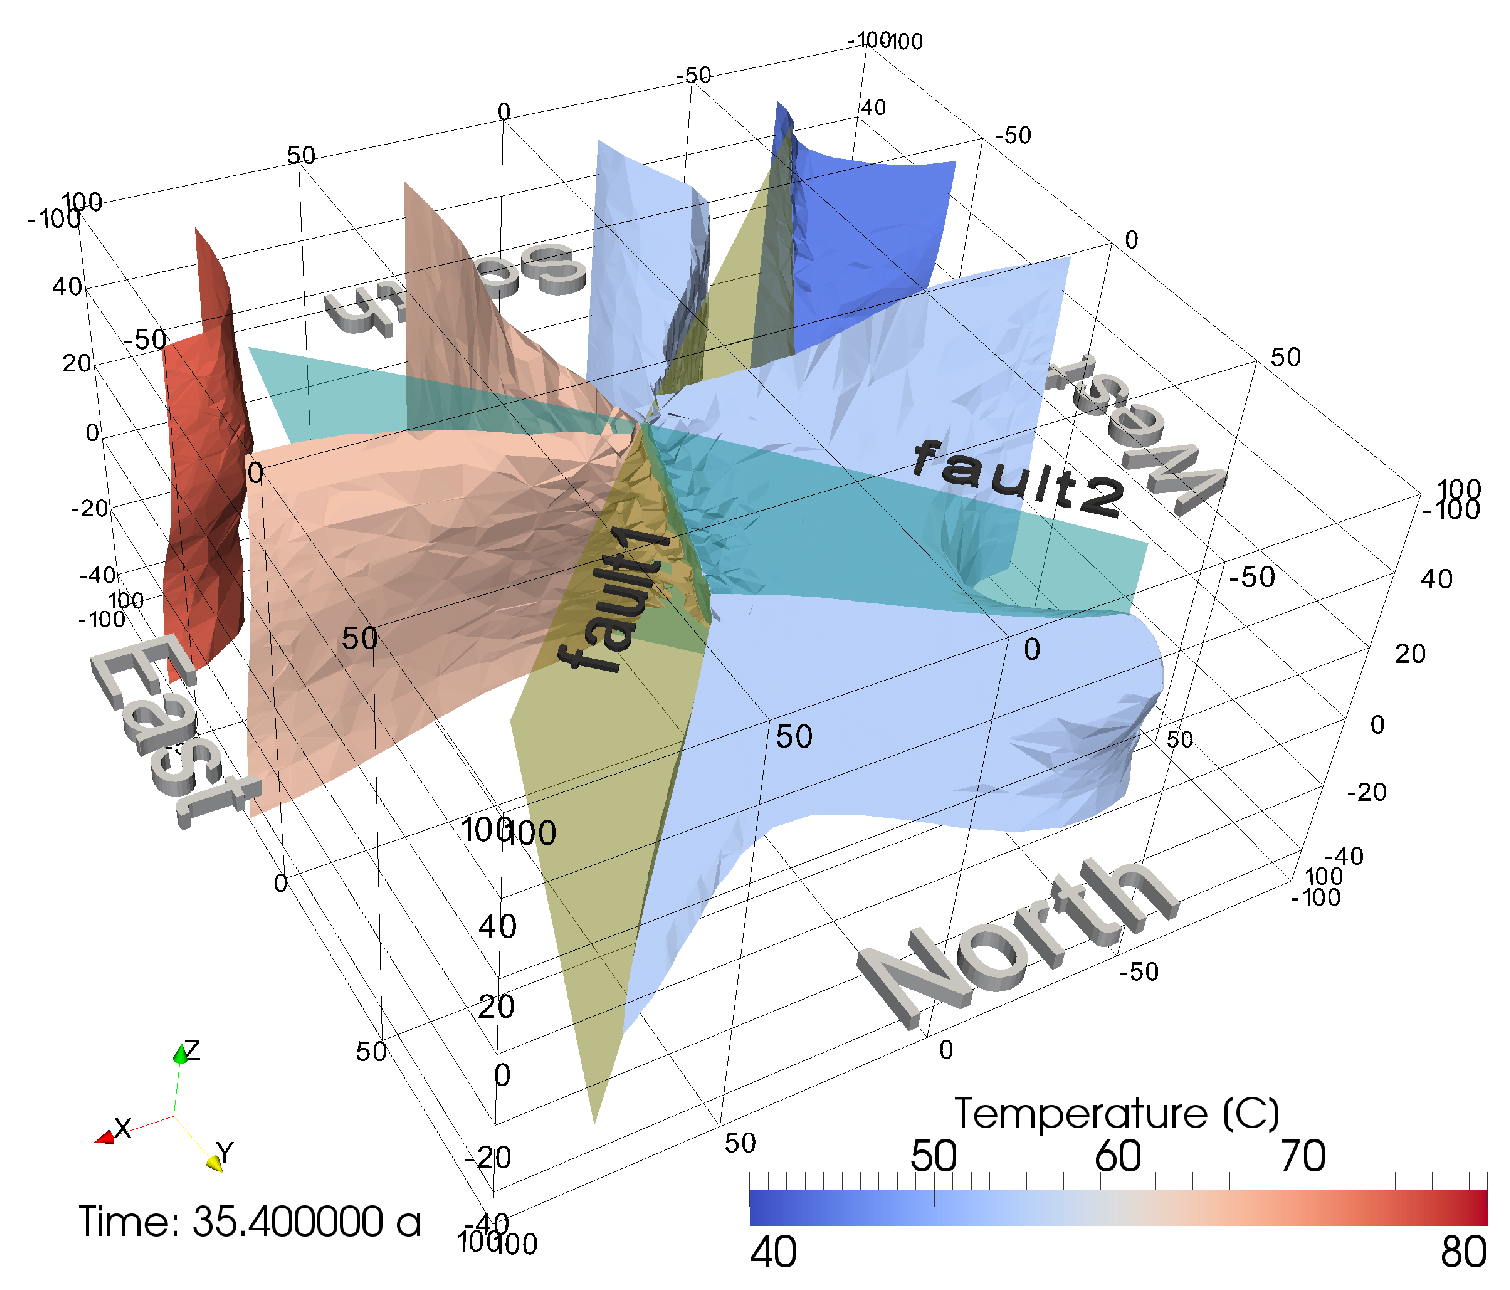
\includegraphics[width=1\textwidth]{T/figures/2u2f_fig5c.eps}
        \end{minipage}
        \begin{minipage}{0.35\textwidth}
            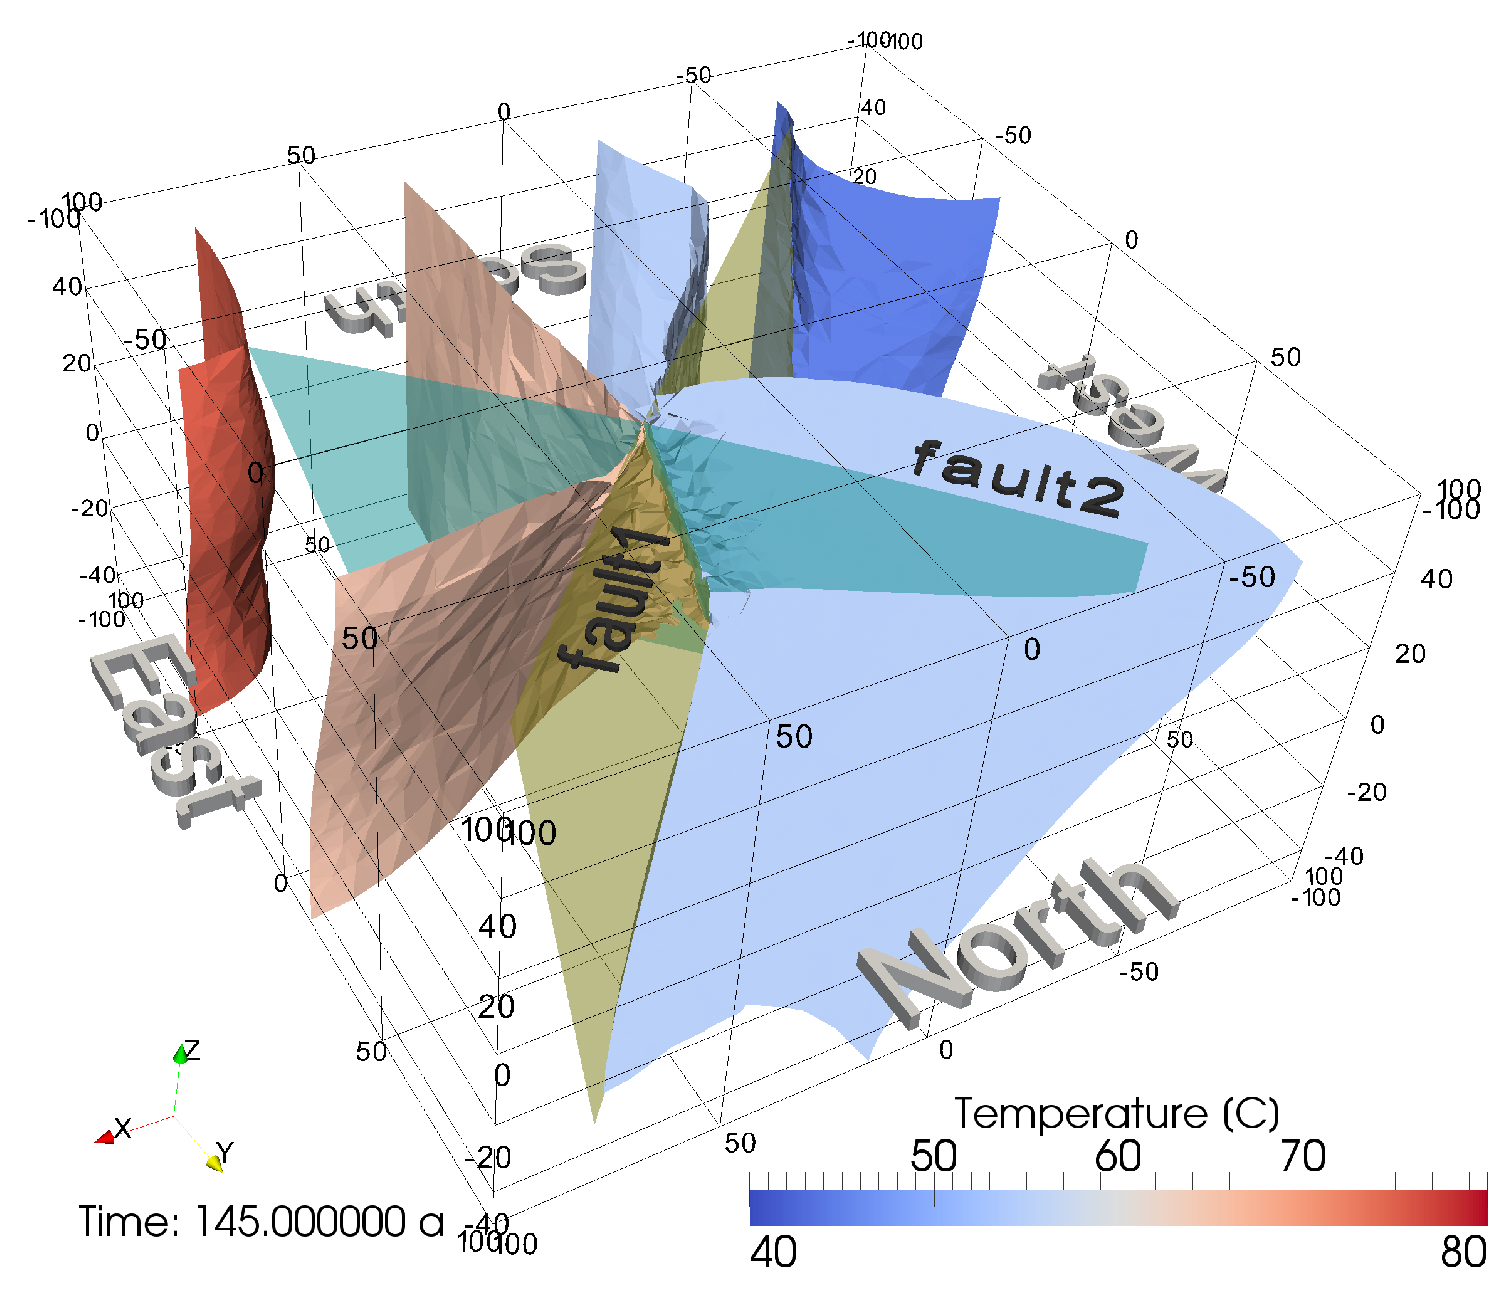
\includegraphics[width=1\textwidth]{T/figures/2u2f_fig5d.eps}
        \end{minipage}
        \caption{Temperature contour plots (45$^\circ{}$C, 55$^\circ{}$C, 65$^\circ{}$C and 75$^\circ{}$C isosurfaces) at four different time stages.}
        \label{fig5}
    \end{center}
\end{figure}

Before stationary field conditions for pressure and velocity are reached, conductive heat transfer does not affect the initial temperature field significantly (Figure \ref{fig5}a). After achieving the stationary pressure and velocity field, convective heat transfer (advection plus diffusion) becomes predominant. The cold water front (T = 55$^\circ{}$C) enters fault 1 after approx. 4 months (Figure \ref{fig5}b). Due to the geometry of fault 1 with respects to the southern boundary of the domain, cold water enters fault 1 in the upper part. After 35 years, (Figure \ref{fig5}c) cold water from fault 1 and hot water from fault 2 are mixed at the fault intersection. The final temperature field (Figure \ref{fig5}d) shows an average temperature of T = 55$^\circ{}$C in the northern part which is less than the mean initial temperature of 60$^\circ{}$C. The depression from the mean value is caused because fault 1 is more conductive than fault 2, which drives higher amounts of cold water into the system.

For a detailed observation of the pressure, velocity and temperature evolution inside the two faults, three observation points were set (Figure \ref{fig6}a).

%figure6
\begin{figure}[htbp]
    \begin{center}
        \begin{minipage}{0.40\textwidth}
            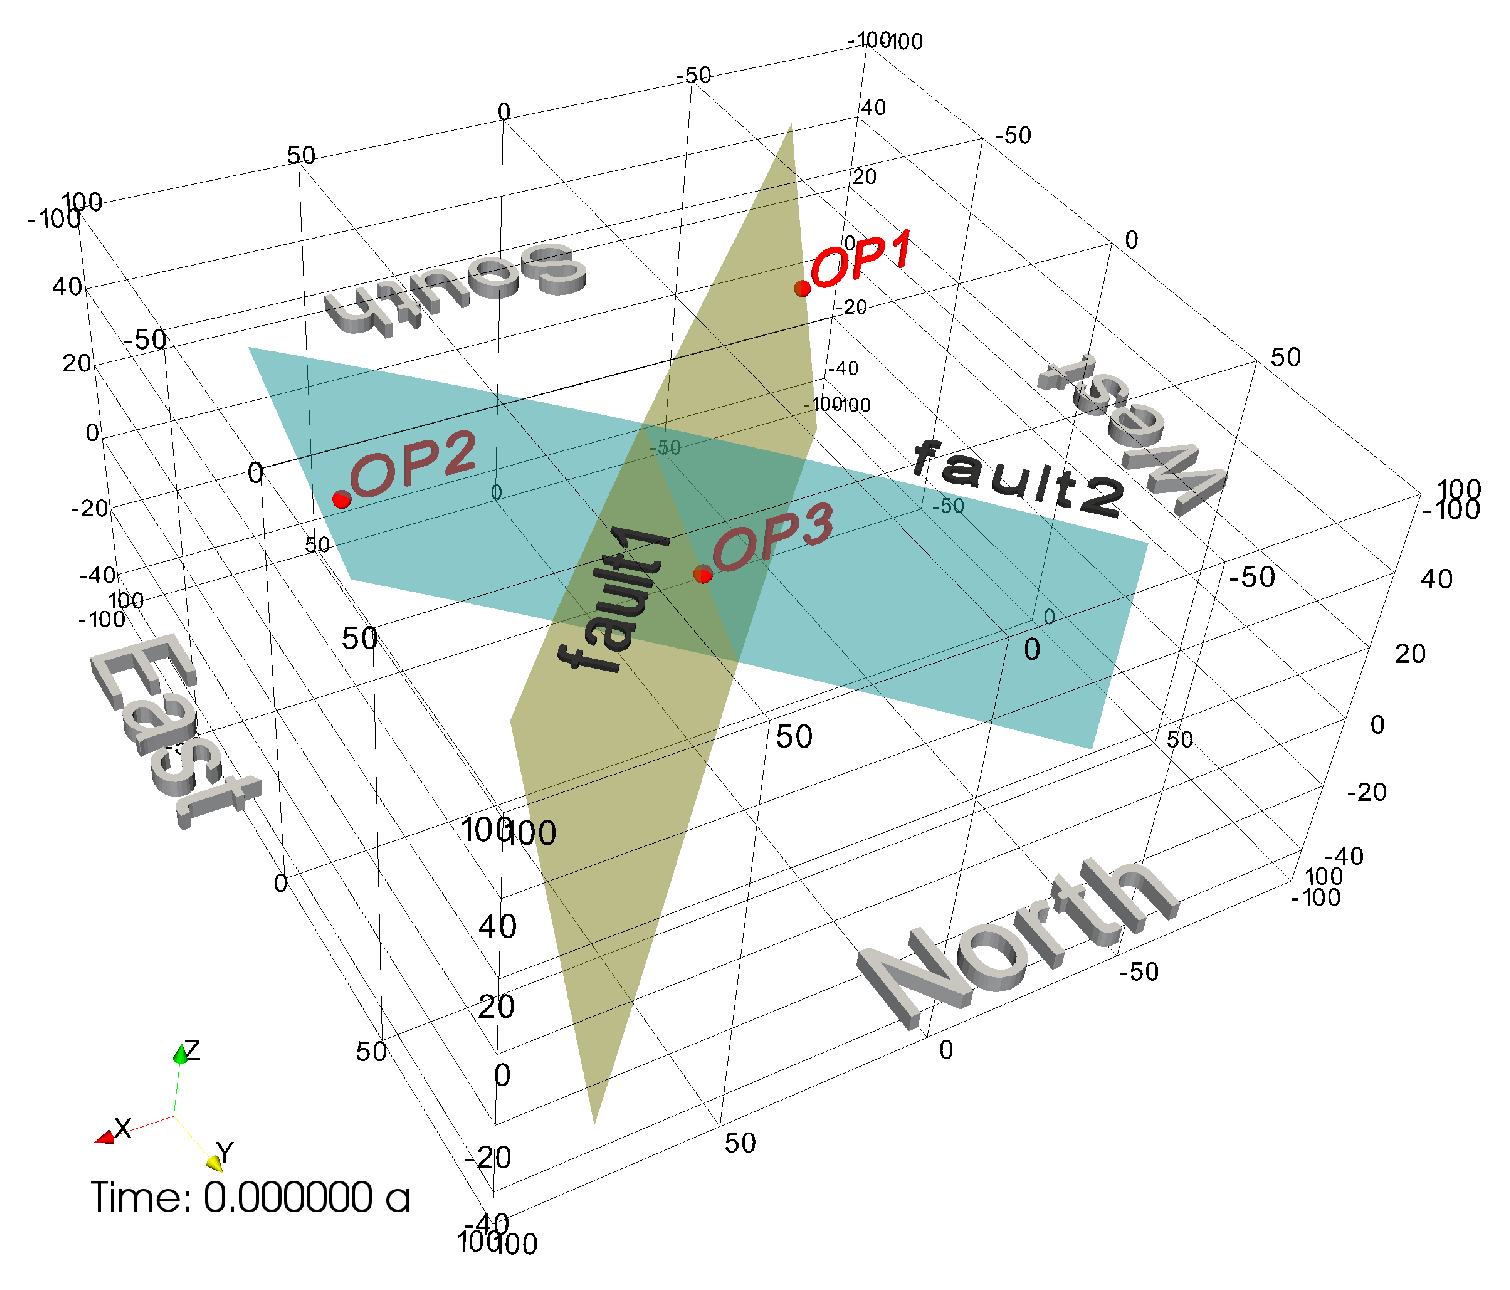
\includegraphics[width=1\textwidth]{T/figures/2u2f_fig6a.eps}
        \end{minipage}
        \begin{minipage}{0.40\textwidth}
            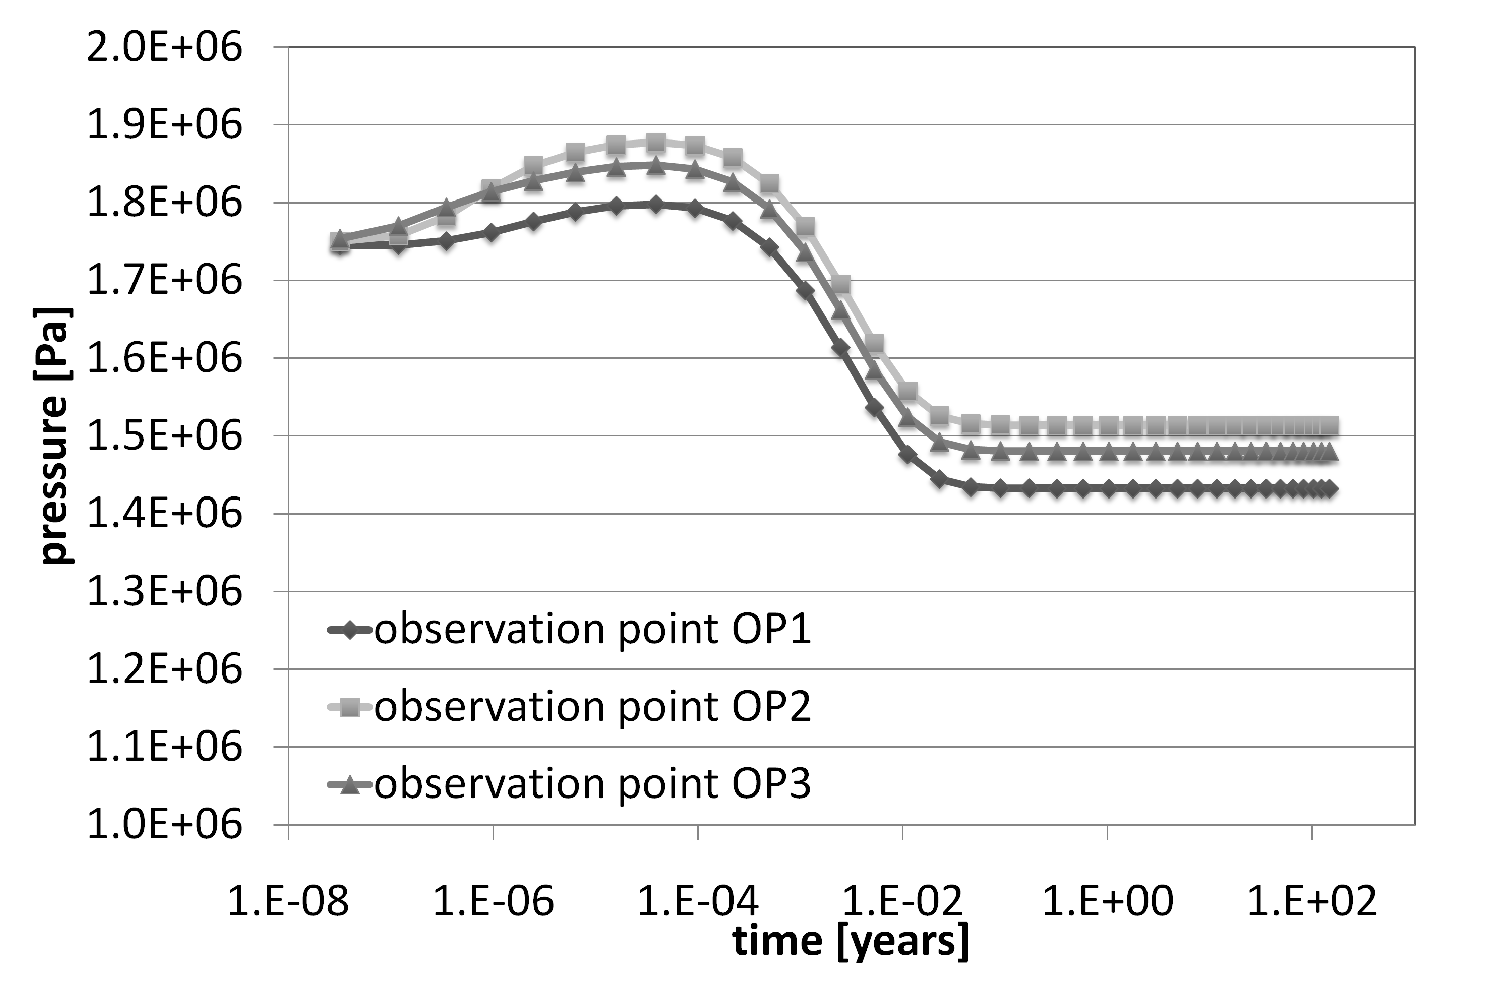
\includegraphics[width=1\textwidth]{T/figures/2u2f_fig6b.eps}
        \end{minipage}
        \begin{minipage}{0.40\textwidth}
            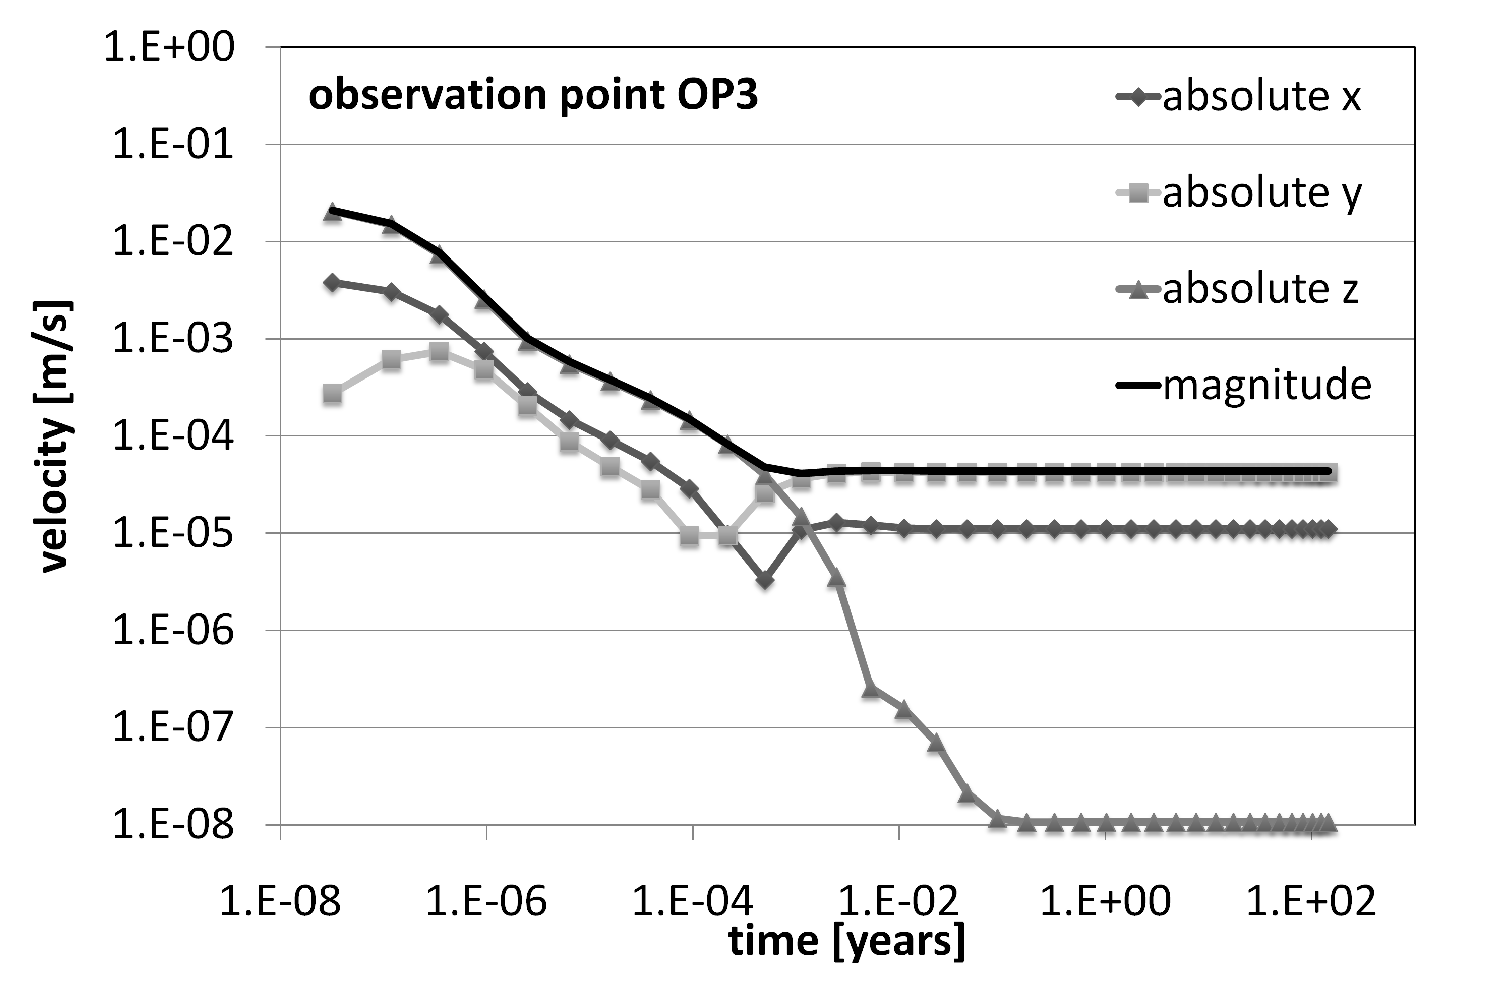
\includegraphics[width=1\textwidth]{T/figures/2u2f_fig6c.eps}
        \end{minipage}
        \begin{minipage}{0.40\textwidth}
            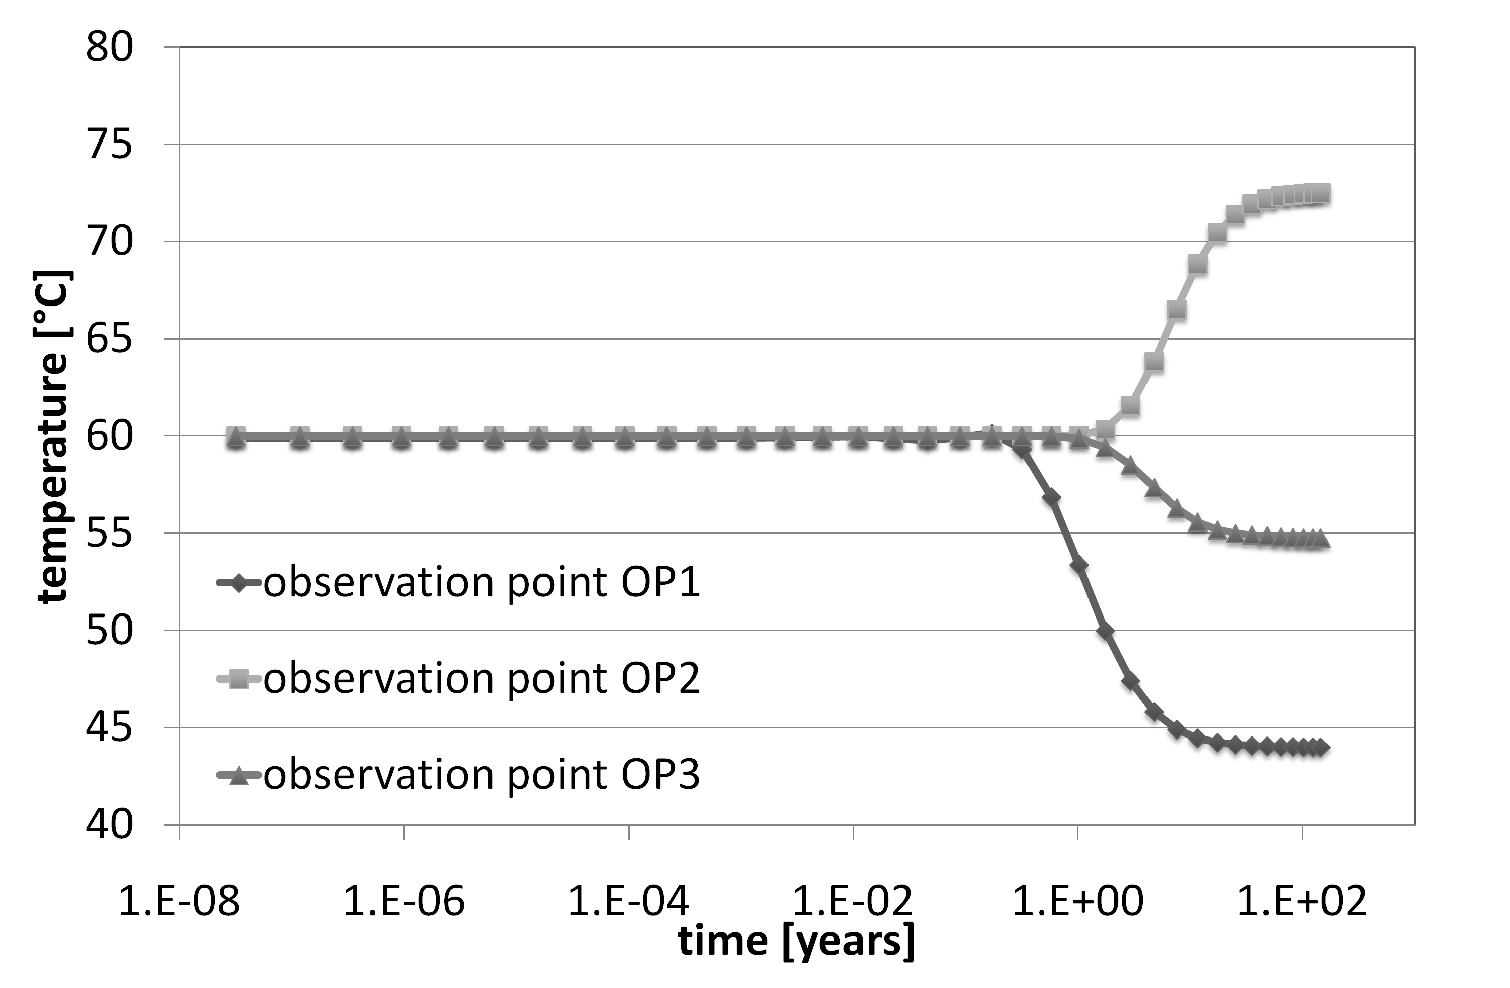
\includegraphics[width=1\textwidth]{T/figures/2u2f_fig6d.eps}
        \end{minipage}
        \caption{Location of three observation points within the fault faces (\ref{fig6}a); Simulated pressure (\ref{fig6}b) and temperature (\ref{fig6}d) values at these observation points and simulated velocity components (\ref{fig6}c) at observation point 3.}
        \label{fig6}
    \end{center}
\end{figure}

After starting the simulation the pressure increases at all observation points (Figure \ref{fig6}b). As shown for observation point 3 (Figure \ref{fig6}c), the initial magnitude of the velocity is due to vertical flow only. The observed downward flow is forced by the initial pressure conditions in combination with the chosen pressure boundary. Therefore, an initial increase of fluid pressure is observed. After 1 month, a stationary pressure and velocity field is reached, as indicated by the horizontal lines in Figure \ref{fig6}b-\ref{fig6}c.

The vertical component of velocity decreases over time from 3$\cdot10^{-2}$ m/s to $10^{-8}$ m/s, and the horizontal flow from the South to the North with velocities between $10^{-5}$ m/s and $10^{-4}$ m/s becomes dominant. The cold water reaches the fault system at the edge of fault 1 (Figure \ref{fig6}d) after approx. 4 month. After an additional 17 months, cooling at observation point 3 begins. At the same time, hot water reaches fault 2 first. Due to the lower transmissivity of fault 2, the hot water reaches the intersection point after 10 years, and cooling at observation point 3 stops. Higher amounts of cold water enter the fault intersection (observation point 3) from the more conductive fault 1, causing temperature to decrease to 55$^\circ{}$C. This corroborates the observation of the temperature field for the total domain.

In a second run, the same problem described above has been numerically solved using the Flux Corrected Transport (FCT) scheme as implemented in Norihiro's branch of OpenGeoSys version 5. Figure \ref{fig7} illustrates the differences regarding numerical oscillations in solving for the transport field with (dashed lines) and without (solid lines) FCT method. Figure \ref{fig7}a and Figure \ref{fig7}b show the calculated temperature profiles along the general flow field for two different stages in the simulation. As shown in Figure \ref{fig7}a, the FCT method seems to reduce the amplitudes of numerical oscillations by a maximum factor of three at the beginning of the simulation. The OGS benchmark files can be found in the subdirectory 2units2faults/FCT.
 
%figure7
\begin{figure}[htbp]
    \begin{center}
        \begin{minipage}{0.72\textwidth}
            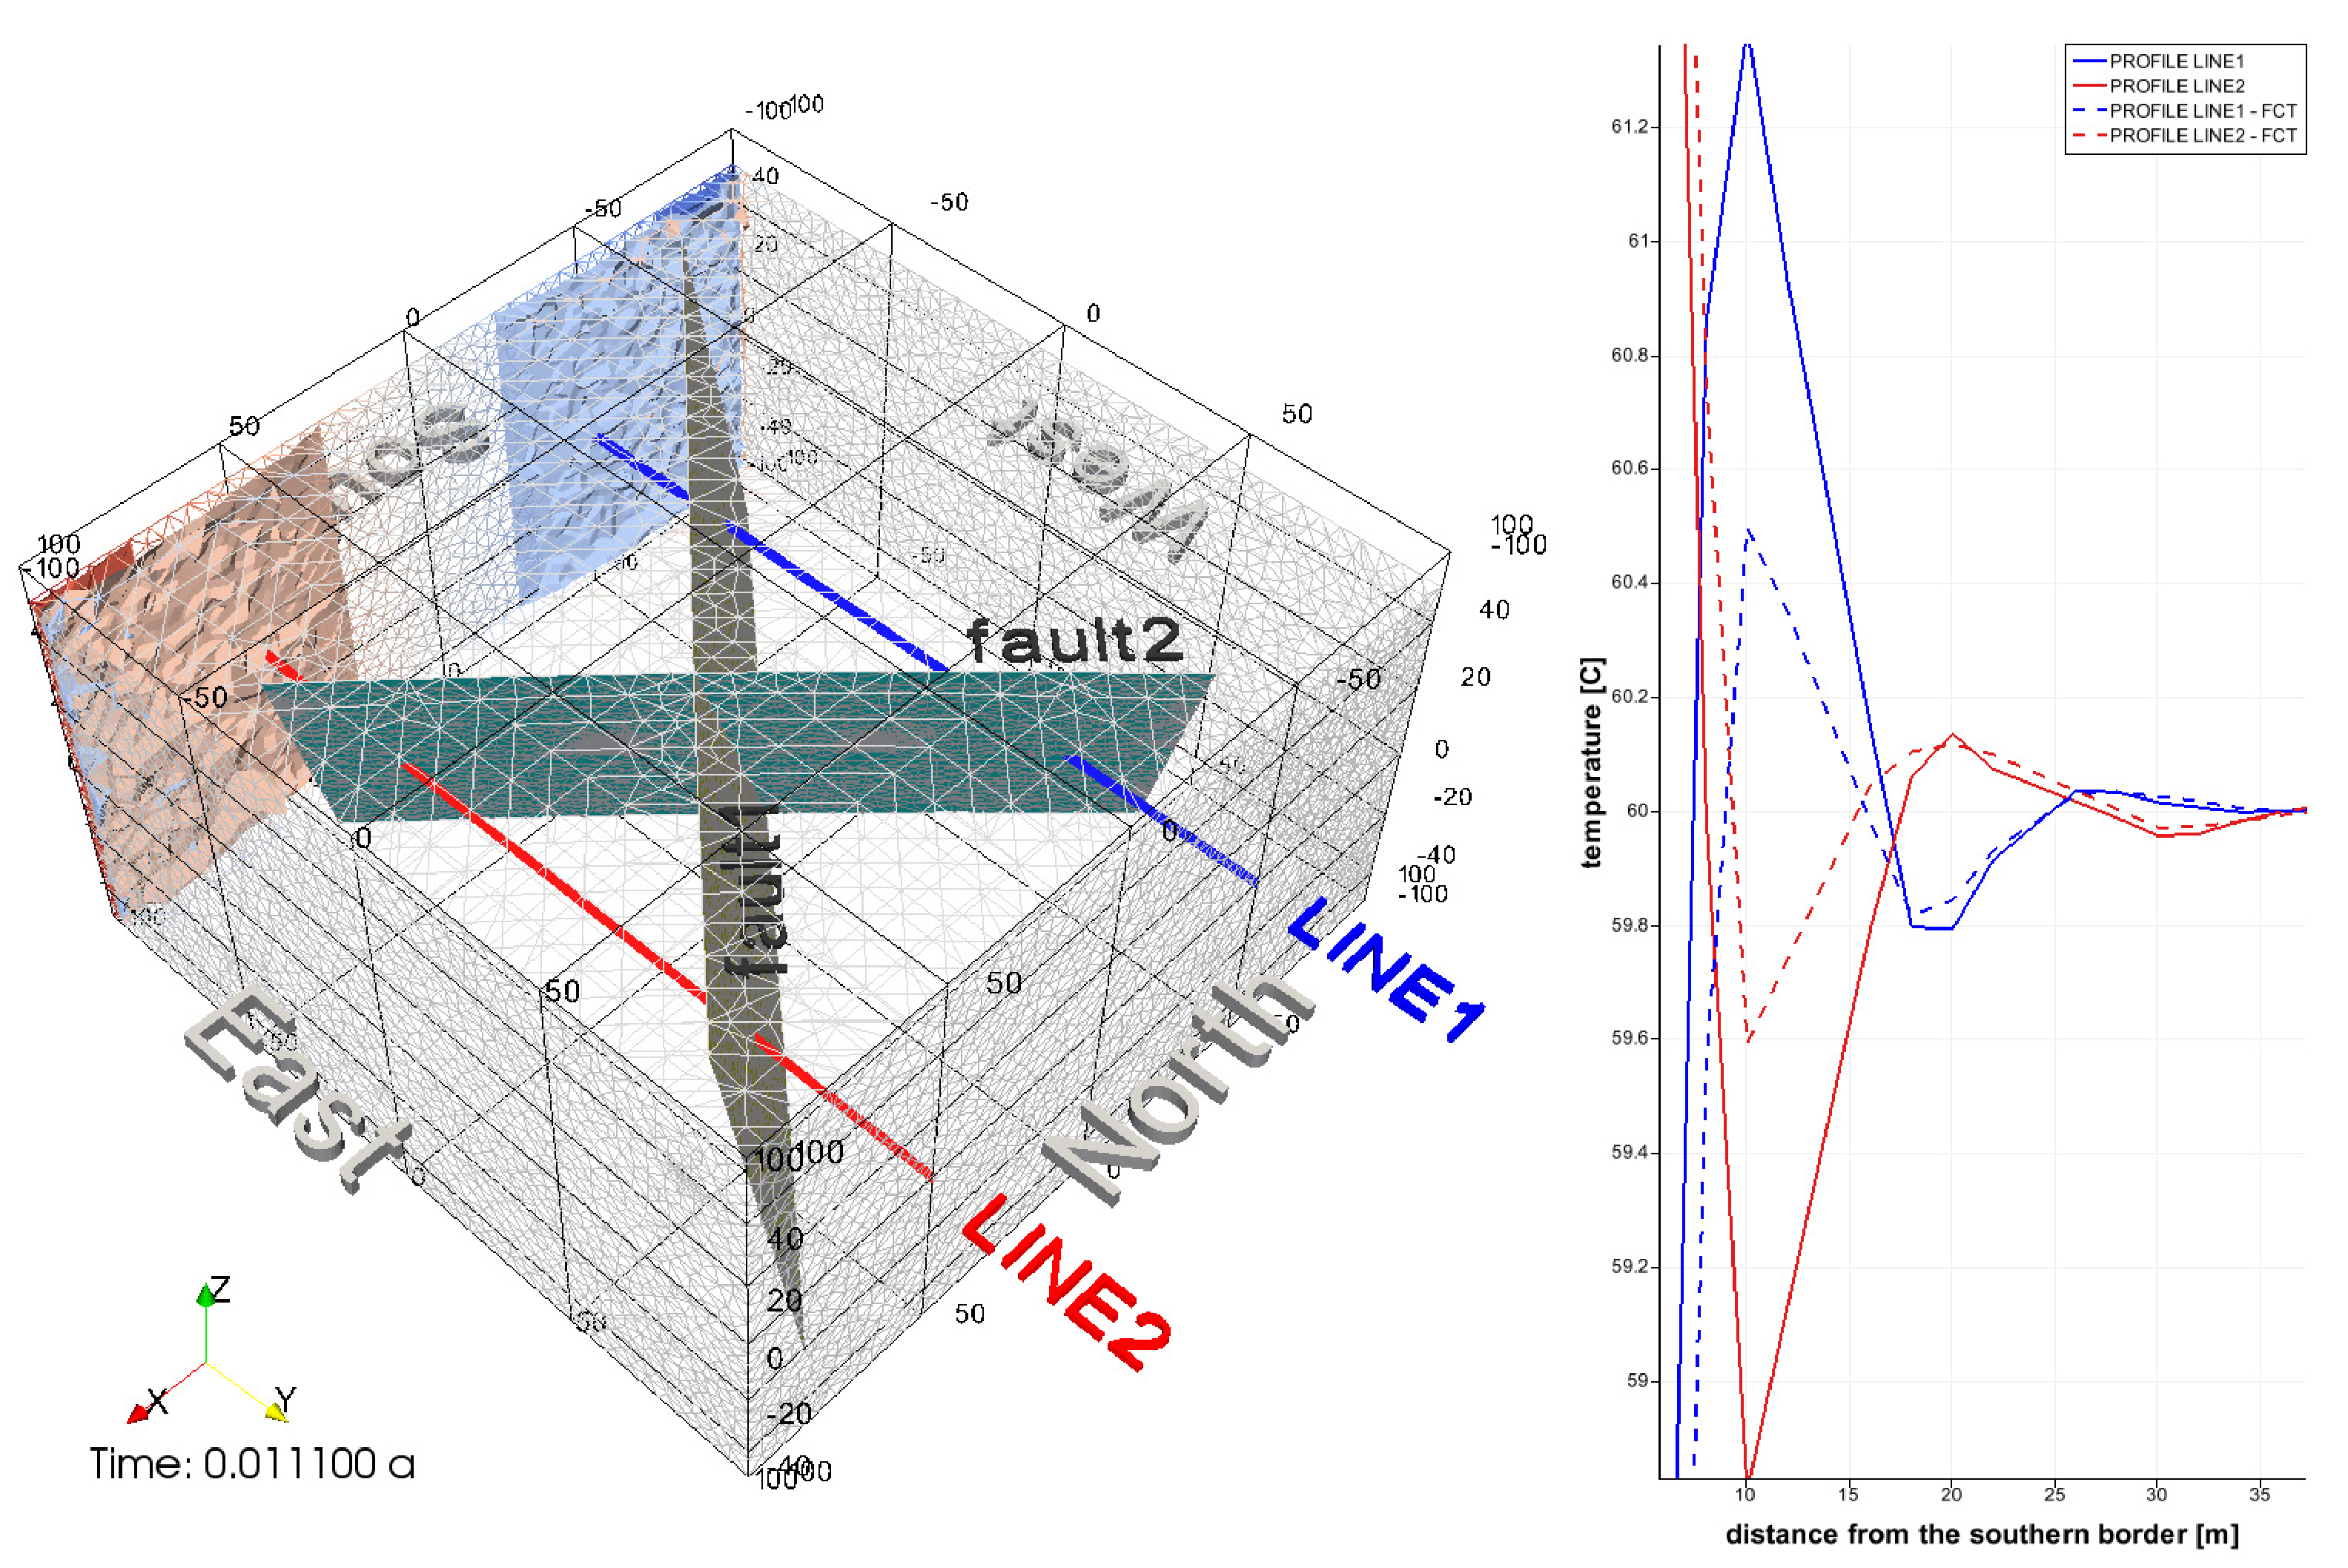
\includegraphics[width=1\textwidth]{T/figures/2u2f_fig7a.eps}
        \end{minipage}
        \begin{minipage}{0.72\textwidth}
            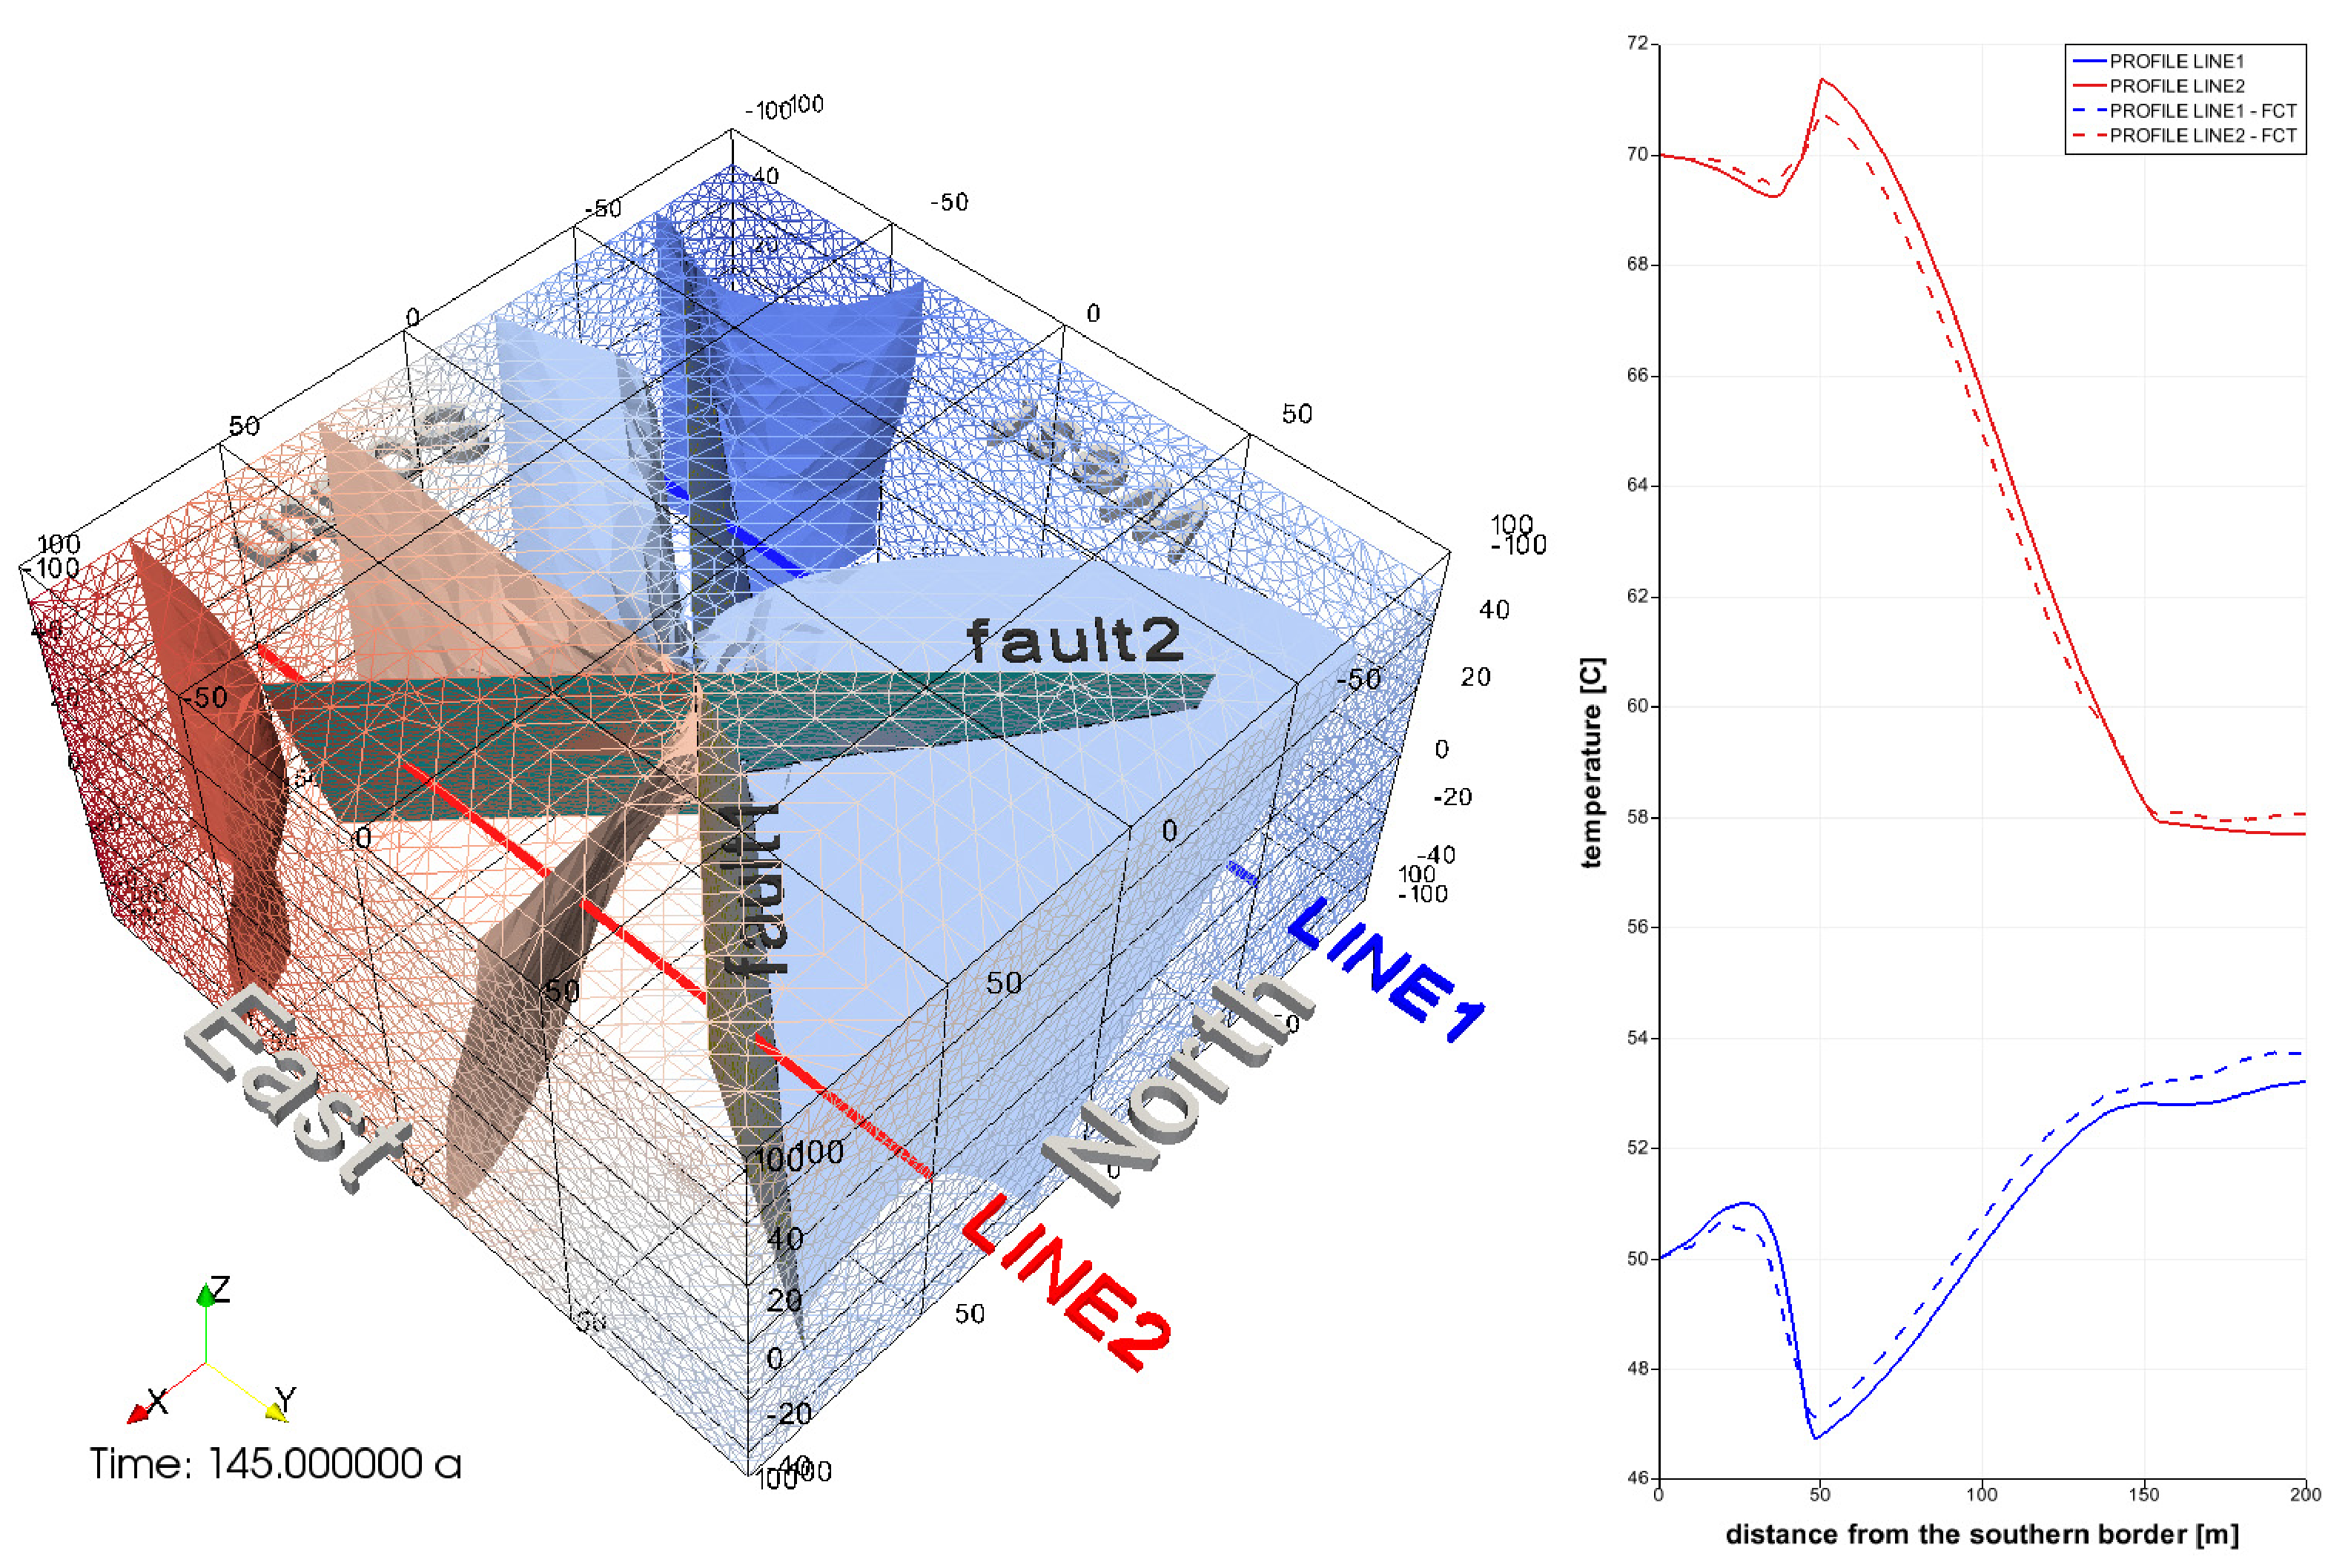
\includegraphics[width=1\textwidth]{T/figures/2u2f_fig7b.eps}
        \end{minipage}
        \caption{Simulated temperature along two lines at the beginning (\ref{fig7}a) and at the final simulation time (\ref{fig7}b) with and without flux corrected transport FCT.}
        \label{fig7}
    \end{center}
\end{figure}




%%%%%%%%%%%%%%%%%%%%%%%%%%%%%%%%%%%%%%%%%%%%%%%%%%%%%%%%%%%%%%%%%%%%%%%%%%%%%%%%%%%%%%%%%%
\section{Heat transport with temperature dependent fluid properties}

\subsection{Problem definition}

A 1D test example for groundwater flow and simultaneous heat transport in the aquifer is made. The aim of the numerical simulation with GeoSys/RockFlow is to determine if the consideration of varying density with temperature changes is possible. The following assumptions will be made:

\begin{tabular}{ll}
Aquifer: & homogeneous, saturated, stationary flow\\
Fluid flow: & incompressible fluid, non-isothermal.\\
\end{tabular}

\subsection{Model set-up of the 1~D numerical model}

For the 1-dimensional calculation the calculation area is simplified as a line of a length of $\unit[5.2]{m}$. The calculation model includes 25 elements and 26 nodes. The initial pressure in the whole area is $\unit[100]{kPa}$ and the initial temperature $\unit[300]{K}$. As boundary condition a constant pressure of $\unit[101]{kPa}$ is given at the left boundary and of $\unit[100]{kPa}$ at the right boundary. A constant temperature of $\unit[400]{K}$ is set at the left boundary. The used soil parameters are listed in Tab.~\ref{tab41}. The fluid density is decreasing with increasing temperature. The viscosity, capacity and conductivity of water are set to constant values. The fluid parameters also can be found in Tab.~\ref{tab41}.
\begin{table}[htbp]
\caption{\label{tab41}Used soil and fluid parameters.}
\begin{center}
\begin{tabular}{ll}
\toprule
parameter 			& value \\
\midrule
\multicolumn{2}{c}{\textit{soil parameters}}\\
porosity $\phi$   	& 0.01 \\	
permeability $K$   	& $\unit[1.0 \cdot 10^{-11}]{m^{2}}$ \\
density $\rho$     	& $\unit[2850]{kg \cdot m^{-3}}$ \\
%heat expansion    	& $\unit[1 \cdot 10^{-5}]{K^{-1}}$ \\
heat capacity $c_s$   	& $\unit[1000]{J \cdot kg^{-1} \cdot K^{-1}}$ \\
heat conductivity $\lambda_s$	& $\unit[3.2]{W \cdot m^{-1} \cdot K^{-1}}$ \\
\cmidrule{1-2}
\multicolumn{2}{c}{\textit{fluid parameters}}\\
initial density $\rho_0$ 	& $\unit[1000]{kg \cdot m^{-3}}$\\
viscosity $\eta$        	& $\unit[0.001]{N \cdot s \cdot m^{-2}}$ \\
heat capacity $c_f$    	& $\unit[4000]{J \cdot kg^{-1} \cdot K^{-1}}$ \\
heat conductivity $\lambda_f$	& $\unit[0.6]{W \cdot m^{-1} \cdot K^{-1}}$ \\
\bottomrule
\end{tabular}
\end{center}
\end{table}

\subsection{Validation method}

In order to find out whether the consideration of varying water density with temperature changes is possible, one simulation run is done with a constant density of $\unit[1000]{kg/m^{3}}$, which is the initial water density before heating, and one run with a constant density of $\unit[900]{kg/m^{3}}$, the density after the heating process. The temperature results for a heat transport with varying density have to be in between both temperature evolution curves.

\subsection{Results}

The curve for temperature evolution, which is shown in Fig.~\ref{figHT1} for the right boundary (node 26), shows the expected characteristics. Therefore it can be stated, that the consideration of temperature dependent fluid density is possible.
\begin{figure}[htbp]
\centering
\includegraphics[width=0.85\textwidth]{T/figures/figHT1.eps}
\caption{\label{figHT1}Temperature evolution with constant and variable fluid densities.}
\end{figure}

\begin{table}[H]
\caption{Benchmark deposit}
\begin{center}
\begin{tabular}{lll}
\toprule
Deposit & Version & Date \\
\midrule
$\backslash$HT\_var\_density\_1D & rf4.7.02 & March 2008\\
\bottomrule
\end{tabular}
\end{center}
\end{table}
%\clearpage


 
\chapter{Groundwater flow -- H-Processes}
\label{sec:Groundwater}
%
This chapter deals with saturated subsurface flow. In the aquifer concept balance equations determine strictly horizontal flow and vertical flow can be included by leakage terms through confining beds. The leakage terms add or subtract water from aquifers overlying and underlying a leaky confining bed according to the aquifer's head difference and a confining bed conductivity. An aquifer which contains a water table is termed unconfined and a completely filled aquifer is termed confined. The governing equations for three-dimensional groundwater, confined, and unconfined aquifer flow are introduced in Sec.~\ref{sec:Groundwater_theory}.
In Sec.~\ref{sec:Groundwater_confined} the benchmarks for confined and in Sec.~\ref{sec:Groundwater_unconfined} for unconfined aquifers are introduced. Groundwater flow is solved two- and three dimensionally in the benchmark examples.

\section{Theory}
\label{sec:Groundwater_theory}
%
A three-dimensional description of groundwater flow is given by the mass balance equation
%
\begin{eqnarray}
S_s\frac{\partial h}{\partial t}
- \nabla\cdot \frac{\rho g}{\mu} {\kappa} \nabla h
= q^{ex}
\label{eqn:GW_Governing}
\end{eqnarray}
%
where the head $h$ is the primary variable of groundwater flow and $S_s$ is the specific storage which is assumed to be independent of the head neglecting fluid and soil matrix compression. Use of Darcy's law for momentum balance leads to the fluid density $\rho$, dynamic fluid viscosity $\mu$, gravity constant $g$, and aquifer permeability matrix ${\kappa}$. Finally $q^{ex}$ denotes external sources and sinks.
Depth integration leads to the two-dimensional Boussinesq equation which describes unconfined aquifers and reads
%
\begin{eqnarray}
S_y\frac{\partial h}{\partial t}
- \nabla\cdot \frac{\rho g h}{\mu}  {\kappa}  \nabla h
= q^{ex}
\label{eqn:GW_unconfinedGoverning}
\end{eqnarray}
%
where $S_y$ is the specific yield.
For confined aquifers Eq.~\ref{eqn:GW_unconfinedGoverning} becomes
%
\begin{eqnarray}
S\frac{\partial h}{\partial t}
- \nabla\cdot \frac{\rho g L}{\mu}  {\kappa}  \nabla h
 = q^{ex}
\label{eqn:GW_confinedGoverning}
\end{eqnarray}
%
where $S$ is the storage and $L$ the aquifer thickness.
The aquifer thickness $L$ is taken into account by changing the soil permeability ${\kappa }$ in the following benchmark examples.
A channel source term can be assigned according to
%
\begin{eqnarray}
q^{ex} = K_{\Lambda} \frac{P}{B}\frac{h^{sur} - h^{sub}}{a}
\label{eqn:GW_riverSource}
\end{eqnarray}
%
where $K_{\Lambda}$ is the channel bed conductivity, $B$ the channel width, $a$ the channel bed thickness, and $h^{sur}$ the channel flow head. The wetted perimeter $P= 2 (h^{sur}-z^{sur}) + B$ for rectangular channel where $z^{sur}$ is the height of the top of the channel bed. Groundwater head $h$ is taken into account by
%
\begin{eqnarray}
h^{sub} = \max\left( h, z^{sur}\right).
\end{eqnarray}
%
Leakage terms between adjacent aquifers can be defined accordingly.
%
%--------------------------------------------------------------------------------------------------------------------------
\section{Linear groundwater flow}


\textbf{Theory}

Water flow in a saturated porous medium is influenced by the pressure gradient over a given distance and the hydraulic conductivity of the aquifer. By Darcy's Law (equ. \ref{eq21}) the flow rate by considering these influences can be calculated.
\begin{equation}
v_f\,=\,k_f\cdot i
\label{eq21}
\end{equation}
{\small
with
\begin{itemize}
\item[$v_f$] -- flow rate (m/s),
\item[$k_f$] -- hydraulic conductivity (m/s),
\item[$i$] -- pressure gradient (-).
\end{itemize}
}

The hydraulic conductivity is calculated by the following relation.
\begin{equation}
k_f\,=\,\frac{\kappa\cdot\rho\cdot g}{\mu}
\label{eq22}
\end{equation}
{\small
with
\begin{itemize}
\item[$\kappa$] -- permeability (m$^2$)
\item[$\rho$] -- density of the fluid (kg$\cdot$m$^{-3}$)
\item[$g$] -- gravity constant (m$\cdot$s$^{-2}$)
\item[$\mu$] -- dynamic viscosity of the fluid (Pa$\cdot$s)
\end{itemize}
}

By using the law of continuity the discharge through a defined cross section can be calculated.
\begin{equation}
Q\,=\,v_f\cdot A
\label{eq23}
\end{equation}
{\small
with
\begin{itemize}
\item[$Q$] -- discharge (m$^3$/s)
\item[$A$] -- cross section (m$^2$)
\end{itemize}
}

Layered soil material is possibly less permeable in one direction than in the direction perpendicular to it. In this case the input of different values for the permeability $\kappa$ in dependence on the direction of anisotropy is possible in RockFlow.


\subsection{Flow in an isotropic medium}


\subsubsection*{Problem definition}

This test example for groundwater flow is taken from the RockFlow Tutorial A (Ma{\ss}mann, 2004). The aim of this example is to simulate the stationary groundwater flow in a homogeneous aquifer. Figure \ref{fig21} shows a sketch of the calculation area.
\begin{figure}[htbp]
\centering
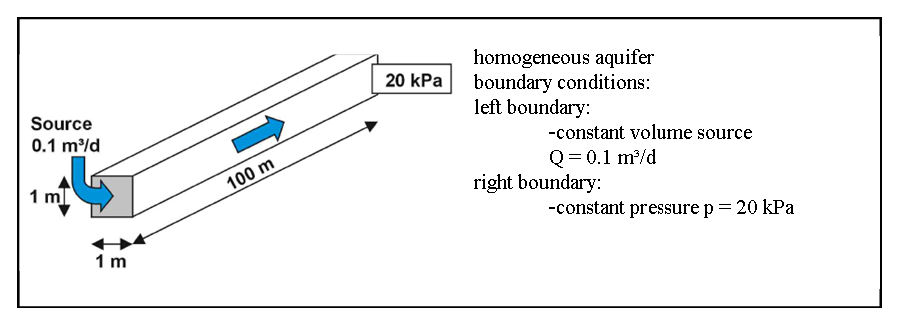
\includegraphics[width=1.0\textwidth]{H_GW/figures/fig21.eps}
\caption{Calculation area: homogeneous aquifer (Ma{\ss}mann, 2004)}
\label{fig21}
\end{figure}

\textsl{Assumptions}

\begin{tabbing}
\=xxxxxxxxxxxxx  \=xxxxxxxxxxxxxxxxxxxxxxx \kill
\> Aquifer: \> homogeneous, saturated, stationary flow
\end{tabbing}

\subsubsection*{Model set-up of the 1~D numerical model}

For the 1-dimensional calculation the calculation area is simplified as a line of a length of 100~m. The calculation model includes 100 elements and 101 nodes. As boundary condition the source volume of the fluid phase of 0.1~m$^3$/d is given at the left border of the calculation area and the constant pressure of 20~kPa at the right boundary. The used parameters of the soil are listed in table \ref{tab21}.
\begin{table}[htbp]
\centering
\begin{tabular}{|c|l|l|}
\hline
parameter & value & unit \\
\hline
porosity $\Phi$  & 0.2 &  --  \\			
\hline
permeability $\kappa$ & 1.0$\cdot 10^{-12}$ & m$^2$ \\
\hline
\end{tabular}
\caption{Used parameters}
\label{tab21}
\end{table}

\subsubsection*{Evaluation method}

The constant flow rate $v_f$ is calculated by using equation \ref{eq23}. In order to calculate the pressure at the left border of the calculation model, Darcy's Law is applied in the following way. The second relation (eq. \ref{eq24}) shows that the pressure gradient is linear.
\begin{equation}
i\,=\,\frac{Q}{k_f\cdot A}\,=\,
\frac{Q}{K\cdot\frac{\displaystyle{\rho\cdot g}}{\displaystyle{\eta}}\cdot A}\,=\,
\frac{1.157\cdot 10^{-6}\,\frac{\displaystyle{\mathrm{m}^3}}{\displaystyle{\mathrm{s}}}}
{9.81\cdot 10^{-6}\,\frac{\displaystyle{\mathrm{m}}}{\displaystyle{\mathrm{s}}}\cdot 1\,\mathrm{m}^2}
\quad\mathrm{and}\quad
p_{\mathrm{left}}\,=\,p_{\mathrm{right}}\,+\,\rho\cdot g\cdot i\cdot l
\label{eq24}
\end{equation}

\begin{figure}[htbp]
\centering
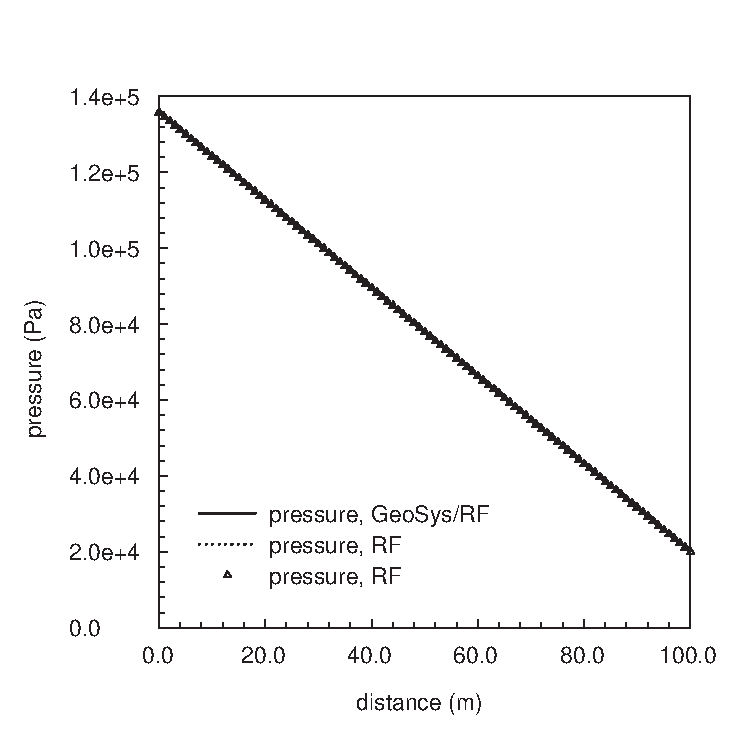
\includegraphics[width=0.5\textwidth]{H_GW/figures/fig22.eps}
\caption{Pressure distribution over the distance of 100~m}
\label{fig22}
\end{figure}

\subsubsection*{Results}

In figure \ref{fig22} you can find the pressure distribution over the whole length of the 1~D model that was calculated by GeoSys/RockFlow. In addition, the analytically calculated pressure distribution is depicted in this figure. These pressure values match the numerical results well.

\begin{tabular}{|l|l|l|}
\hline
Benchmark & Problem type	& Path in benchmark deposit \\
\hline	
h\_sat\_flow\_1d	& H	& benchmarks $\backslash$H$\backslash$sat\_1D \\
\hline	
\end{tabular}


\subsection{Flow in an anisotropic medium}


\subsubsection*{Problem definition}

The aim of this example is to simulate the stationary groundwater flow in an anisotropic porous medium. In order to consider the anisotropy of permeability, a 2~D numerical model was built which contains a higher permeability in the vertical than in the horizontal direction.

\textsl{Assumptions}

\begin{tabbing}
\=xxxxxxxxxxxxx  \=xxxxxxxxxxxxxxxxxxxxxxx \kill
\> Aquifer: \> anisotropic, saturated, stationary flow
\end{tabbing}

\subsubsection*{Model set-up of the 2~D numerical model}

For the 2-dimensional simulation, the cube consisting of a porous medium is simplified as a square with an area of 1~m$^2$. The calculation model includes 736 triangular elements and 409 nodes. At the left corner at the bottom of the model a constant pressure of 1000~Pa is specified along two polylines of the length of 0.3~m (\ref{fig23}). At the top and the right border the pressure is set to 0 in order to create a pressure gradient. As the porous medium is assumed to be anisotropic, which influences the groundwater flow, the values for permeability are equal to 1.0$\cdot 10^{-15}$ m$^2$ in x-direction and 1.0$\cdot 10^{-14}$ m$^2$ in y-direction.

\begin{table}[htbp]
\centering
\begin{tabular}{|c|l|l|}
\hline
parameter & value & unit \\
\hline
porosity $\Phi$  & 0.2 &  --  \\			
\hline
permeability $\kappa_x$ & 1.0$\cdot 10^{-15}$ & m$^2$ \\
\hline
permeability $\kappa_y$ & 1.0$\cdot 10^{-14}$ & m$^2$ \\
\hline
\end{tabular}
\caption{Used parameters}
\label{tab22}
\end{table}

\begin{figure}[htbp]
\centering
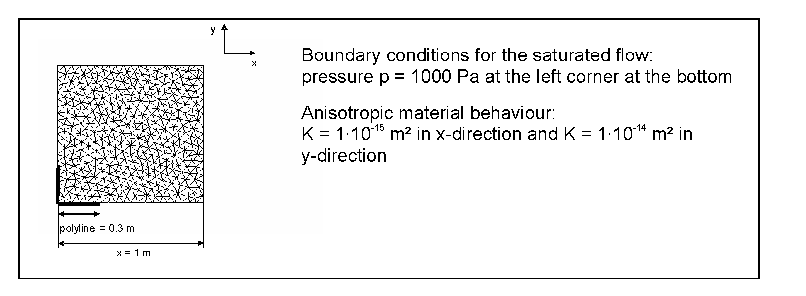
\includegraphics[width=1.0\textwidth]{H_GW/figures/fig23.eps}
\caption{Calculation model (2~D)}
\label{fig23}
\end{figure}

\subsubsection*{Evaluation method}
This test example is not made up to introduce a new process, but it shows the possibility for the GeoSys/RockFlow user to give a specific permeability for each direction. Therefore, the interpretation of GeoSys/RockFlow results comprises merely the comparison between pressure distributions due to anisotropic groundwater flow that were simulated by the use of RockFlow and GeoSys/RockFlow. This comparison is possible because both versions are developed separately concerning anisotropy of soils.

\begin{figure}[htbp]
\centering
\includegraphics[width=0.6\textwidth]{H_GW/figures/fig24.eps}
\caption{Pressure distribution caused by anisotropic saturated flow}
\label{fig24}
\end{figure}

\subsubsection*{Results}

In figure \ref{fig24} the horizontal and vertical pressure distributions of an anisotropic groundwater model which is made using the program code RockFlow are depicted next to the pressure distributions of the described anisotropic model. While presuming an anisotropic medium, an inhomogeneous pressure field is developing, because the groundwater is not able to spread out uniformly. This can be recognized at the different curve gradients in x- and y-direction. There are slight differences between the curve characteristics of the RockFlow and the GeoSys/RockFlow simulation results. These differences are due to different element types (square in the RockFlow model) and the resulting differing x- or y-coordinates. Therefore, the pressure distributions that are obtained by the simulation with GeoSys/RockFlow are evaluated to be correct.

\begin{tabular}{|l|l|l|}
\hline
Benchmark & Problem type	& Path in benchmark deposit \\
\hline	
H\_sat\_flow\_K\_ortho	& H	& benchmarks $\backslash$H$\backslash$sat\_2D \\
\hline	
\end{tabular}


\subsection{Flow in an isotropic and heterogeneous medium}


\subsubsection*{Problem definition}

The aim of this example is to simulate the stationary groundwater flow in an isotropic and heterogeneous porous medium. In order to consider the heterogeneous of permeability, a 2~D numerical model was built. The heterogeneous distribution of permeability is showed in \ref{KDis}.
\begin{figure}[htbp]
\centering
\includegraphics[width=0.8\textwidth]{H_GW/figures/KDis.eps}
\caption{Calculation model(2~D): hetergeneous permeability distribution}
\label{KDis}
\end{figure}

\textsl{Assumptions}

\begin{tabbing}
\=xxxxxxxxxxxxx  \=xxxxxxxxxxxxxxxxxxxxxxx \kill
\> Aquifer: \> isotropic, heterogeneous, saturated, stationary flow
\end{tabbing}

\subsubsection*{Model set-up of the 2~D numerical model}

For the 2-dimensional simulation, the cube consisting of a porous medium is simplified as a square with an area of 10000~m$^2$. The calculation model includes 10000 quad elements and 10201 nodes. At the left boundary  a constant head of 10~m and the right boundary  a constant head of 9~m are specified in order to create a pressure gradient. 

\subsubsection*{Results}

In figure \ref{HeadDis} the horizontal and vertical head distributions of a groundwater flow in a heterogeneous medium are depicted responsing to the distribution of the permeability. 

\begin{figure}[htbp]
\centering
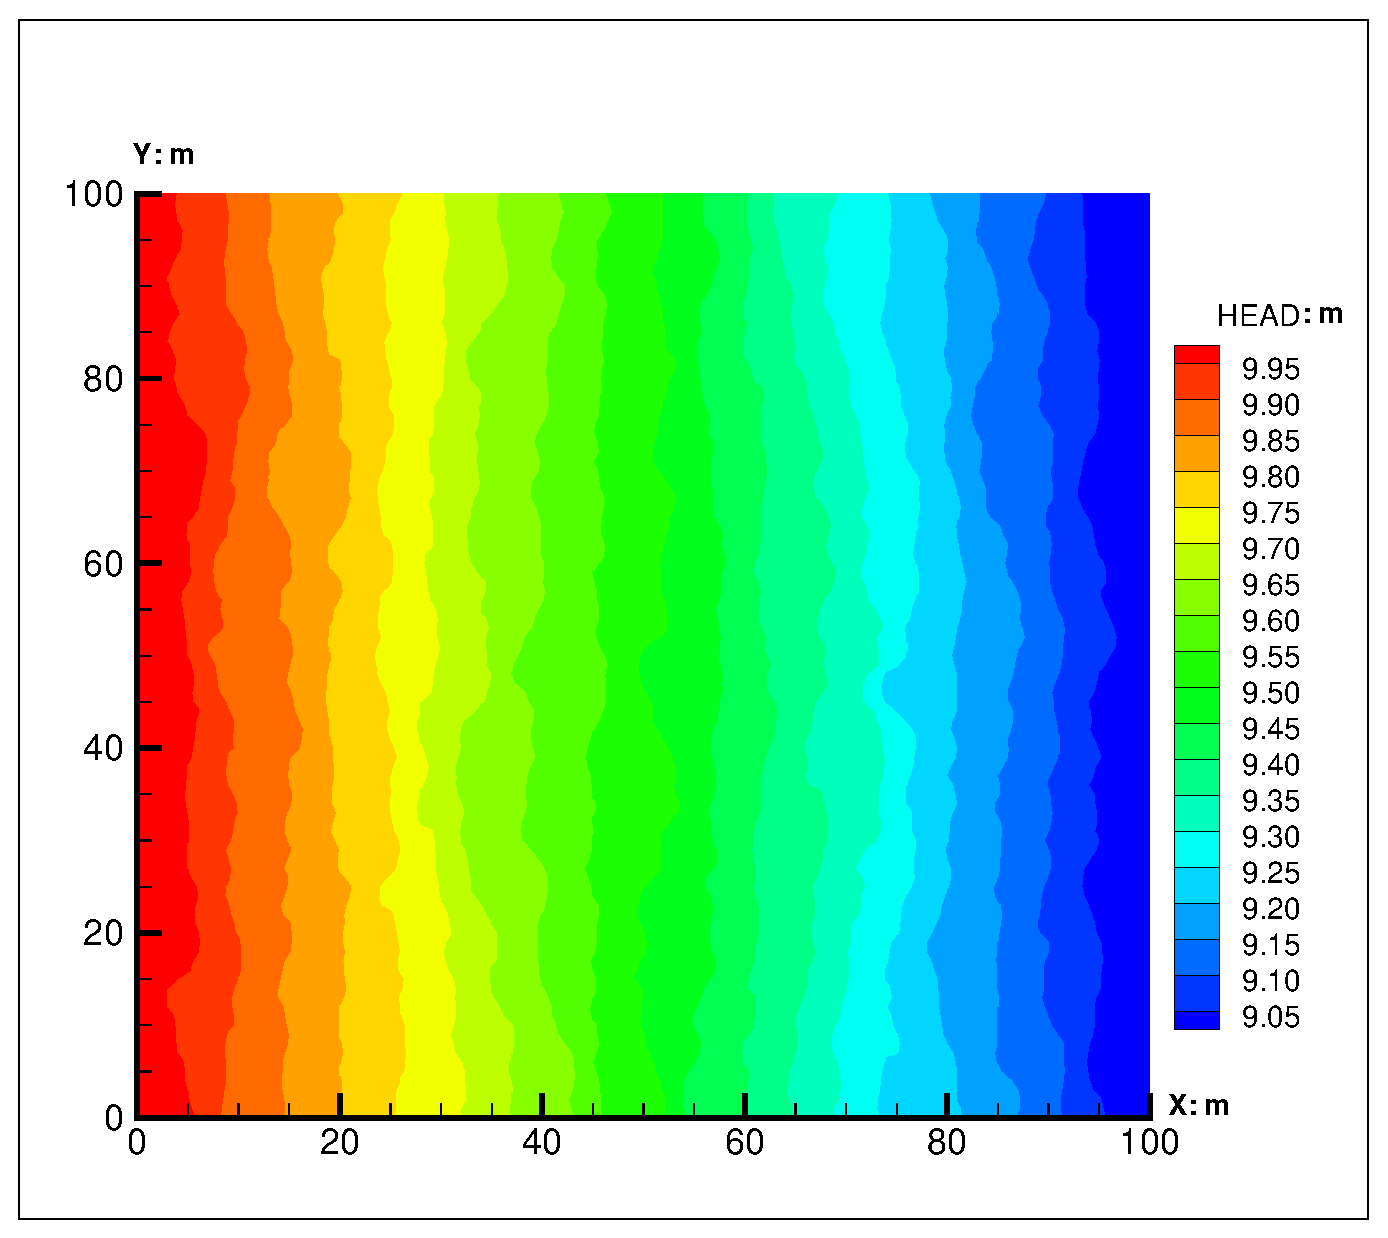
\includegraphics[width=0.8\textwidth]{H_GW/figures/HeadDis.eps}
\caption{Head distribution responsed to isotropic and heterogeneous medium}
\label{HeadDis}
\end{figure}

\begin{tabular}{|l|l|l|}
\hline
Benchmark & Problem type	& Path in benchmark deposit \\
\hline	
2D1P-GWFlow	& H	& benchmarks $\backslash$H$\backslash$HetGWFlow \\
\hline	
\end{tabular}
%--------------------------------------------------------------------------------------------------------------------------
%
\section{Confined aquifer}
\label{sec:Groundwater_confined}
%
%--------------------------------------------------------------------------------------------------------------------------
\subsection{Constant source term}
\label{sec:Groundwater_confined_source}
%
\subsubsection*{Problem definition}
%
These examples deal with an aquifer which is subject to a constant recharge line source.
\cite{Glover:78} presented an analytical solution for a constant line source on an infinite domain which reads for the groundwater head at the source
%
\begin{eqnarray}
h = q^{ex}\sqrt{ \frac{\mu t}{\pi \rho g k L S_y}}. \label{GW_Glover}
\end{eqnarray}
%
The aquifer size is $20m\times 10m$ with the source term at one boundary (See Fig.~\ref{GW_riv1_domain}). The simulation time is $30min$.
%
\subsubsection*{Initial and boundary conditions}
%
Initial groundwater head is $0m$. The source term is $2\times 10^{-4} m/s$, groundwater head is $0$ at the opposite boundary, and at the remaining part no-flow is imposed.
\subsubsection*{Material properties}
%
For the spatial discretization $24\times 12$ quadrants or hexahedra are used. The hexahedra have a height of $1m$.
Material parameters are given in Tab.~\ref{GW_SourceTerm}.
%
\begin{table}[H]
 \centering
 \caption{Parameters for the constant source term examples}
 \centering \label{GW_SourceTerm}
 \begin{tabular}{llll}
 \hline\hline\noalign{\smallskip}
 {\bf Parameter} & {\bf Symbol} & {\bf Setting} & {\bf Unit} \\ \hline
 Storage & $S$ & $0.2$ & $-$ \\
 Specific storage & $S_s$ & $0.2$ & $1/m$ \\
 Viscosity  & $\mu$ & $1\times 10^{-3}$ & $Pa\cdot s$\\
 Thickness & $L$ & $1$ & $m$ \\
 \noalign{\smallskip}\hline\hline
 \end{tabular}
\end{table}
%
\subsubsection*{Results}
%
Simulation results are compared with the analytical solution in Fig.~\ref{GW_Results_Source}
%
\begin{figure} [htb!]
 \centering
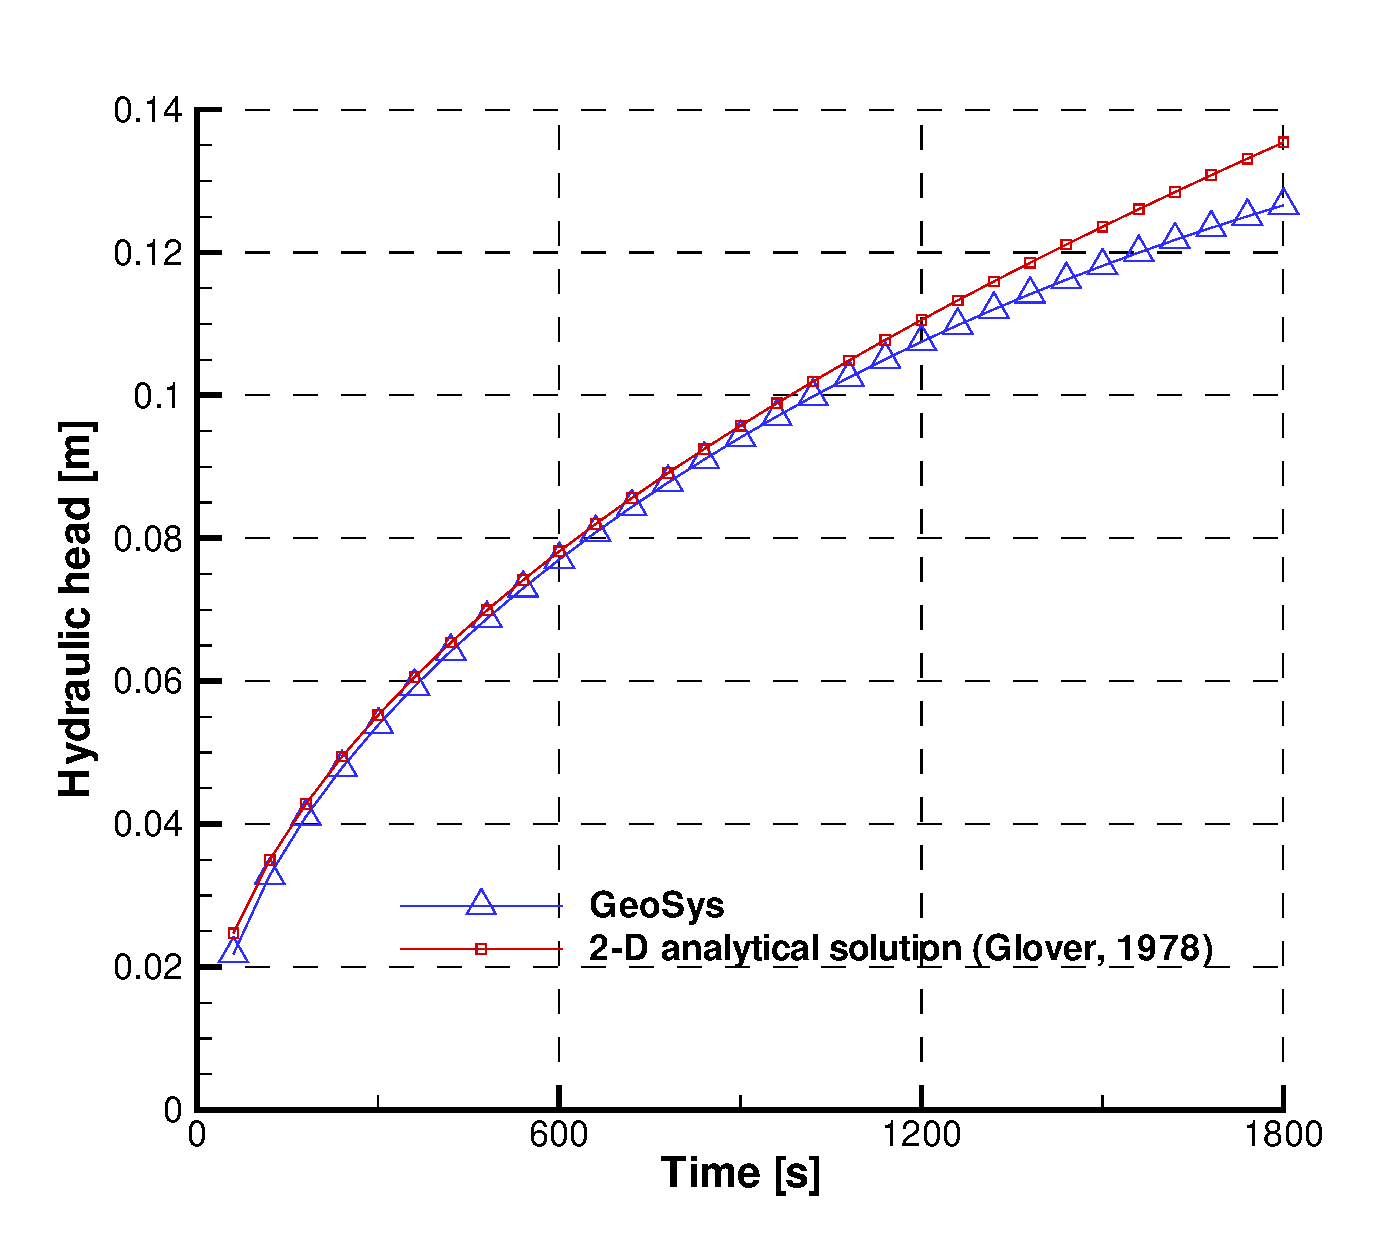
\includegraphics[width=0.6\columnwidth] {H_GW/figures/q_hex_point.eps}
\caption{Results and analytical solution for confined aquifer with line source term}
 \label{GW_Results_Source}
\end{figure}
%
\subsubsection*{Benchmark deposit}
%
\begin{tabular}{|l|l|l|}
  \hline
  Benchmark & Problem type & Path in benchmark deposit \\
  \hline
  \emph{q\_quad} & H & benchmarks\verb \GROUNDWATER_FLOW\ \\
  \emph{q\_hex} & H & benchmarks\verb \GROUNDWATER_FLOW\ \\
  \hline
\end{tabular}
%
%--------------------------------------------------------------------------------------------------------------------------
%
\subsection{Channel source term}
\label{sec:Groundwater_confined_channelSource}
%
\subsubsection*{Problem definition}
%
For these examples the source term of the previous examples (Sec.~\ref{sec:Groundwater_confined_source}) is substituted by a corresponding channel source term (Eqn.~\ref{eqn:GW_riverSource}). The channel is assumed to be not affected by the water loss and the exchange flux is independent of the groundwater head. Therefore, the source term represents a steady and uniform channel located above the aquifer. The cross-section of the channel is rectangular. The setup, spatial discretization, and calculated water head are shown in Fig.~\ref{GW_riv1_domain}. The simulation time is $30min$.
%
\begin{figure} [htb!]
 \centering
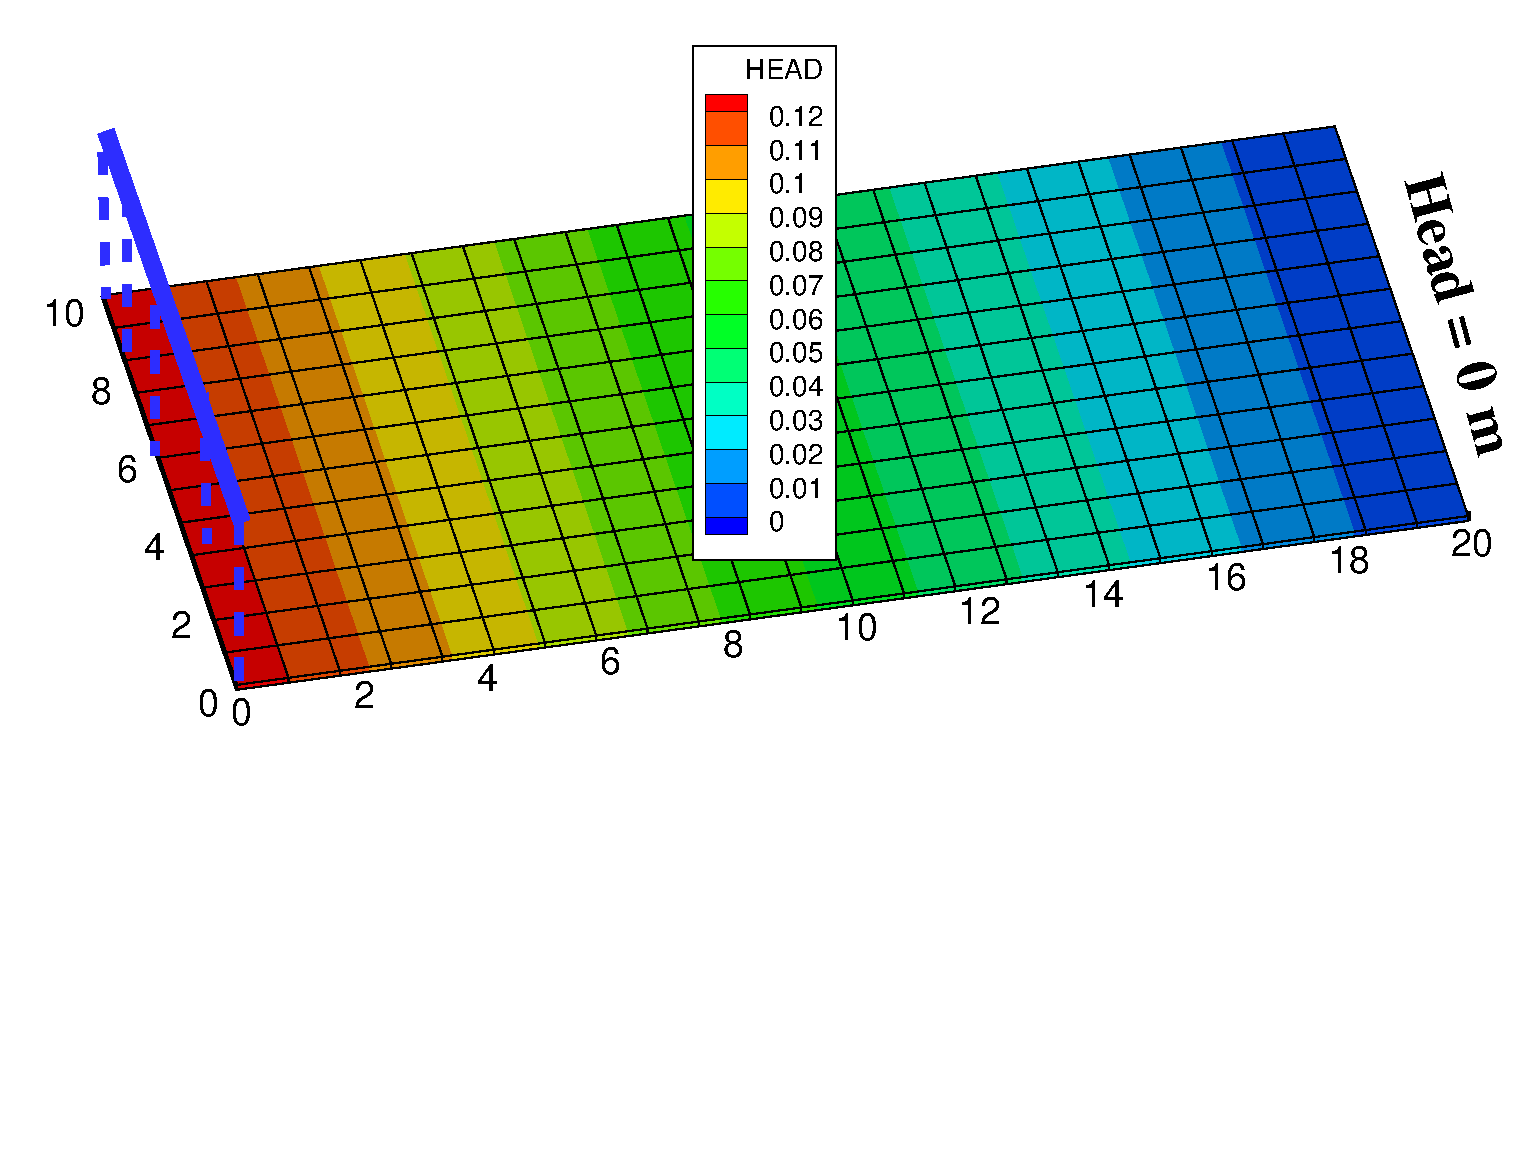
\includegraphics[width=0.7\columnwidth] {H_GW/figures/q_hex.eps}
\vspace{-2cm}
\caption{Computational domain and (channel) source term location}
 \label{GW_riv1_domain}
\end{figure}

%
\subsubsection*{Initial and boundary conditions}
%
The initial groundwater head is $0m$. The channel source term is the boundary condition at one side, at the opposite boundary the head is fixed $0$. At the remaining boundaries no-flow is imposed.
\subsubsection*{Material properties}
%
For the spatial discretization either $24\times 12$ quadrants or hexahedra are used as well prisms which are generated by cutting the hexahedra in two parts. The hexahedra or prism height is $1m$. The time step is $1 min$.
Simulation parameters for the aquifer and the channel source term are given in Tab.~\ref{GW_ChannelPercolation}.
%
\begin{table}[H]
 \centering
 \caption{Parameters for channel source term examples}
 \centering \label{GW_ChannelPercolation}
 \begin{tabular}{llll}
 \hline\hline\noalign{\smallskip}
  {\bf Parameter} & {\bf Symbol} & {\bf Setting} & {\bf Unit} \\ \hline
 {\bf Aquifer} & & & \\
 Storage & $S$ & $0.2$ & $-$ \\
 Specific storage & $S_s$ & $0.2$ & $1/m$ \\
 Viscosity  & $\mu$ & $1\times 10^{-3}$ & $Pa\cdot s$\\
 Thickness & $L$ & $1$ & $m$ \\ \hline
 {\bf Channel source term} & & & \\
 Head & $h^{sur}$ & $4$ & $m$ \\
 Bed top location& $z^{sur}$ & $1$ & $m$ \\
 Width & $B$ & $14$ & $m$ \\
 Conductivity & $K_{\Lambda}$ & $1\times 10^{-6}$ & $m/s$ \\
 Thickness & $a$ & $0.3$ & $m$ \\
 \noalign{\smallskip}\hline\hline
 \end{tabular}
\end{table}
%
\subsubsection*{Results}
%
Comparison of simulation results and analytical solution is given in Fig.~\ref{GW_Results_ChannelPercolation_quad}
for quadrants and in Fig.~\ref{GW_Results_ChannelPercolation_hex} for hexahedra.
%
\begin{figure} [htb!]
 \centering
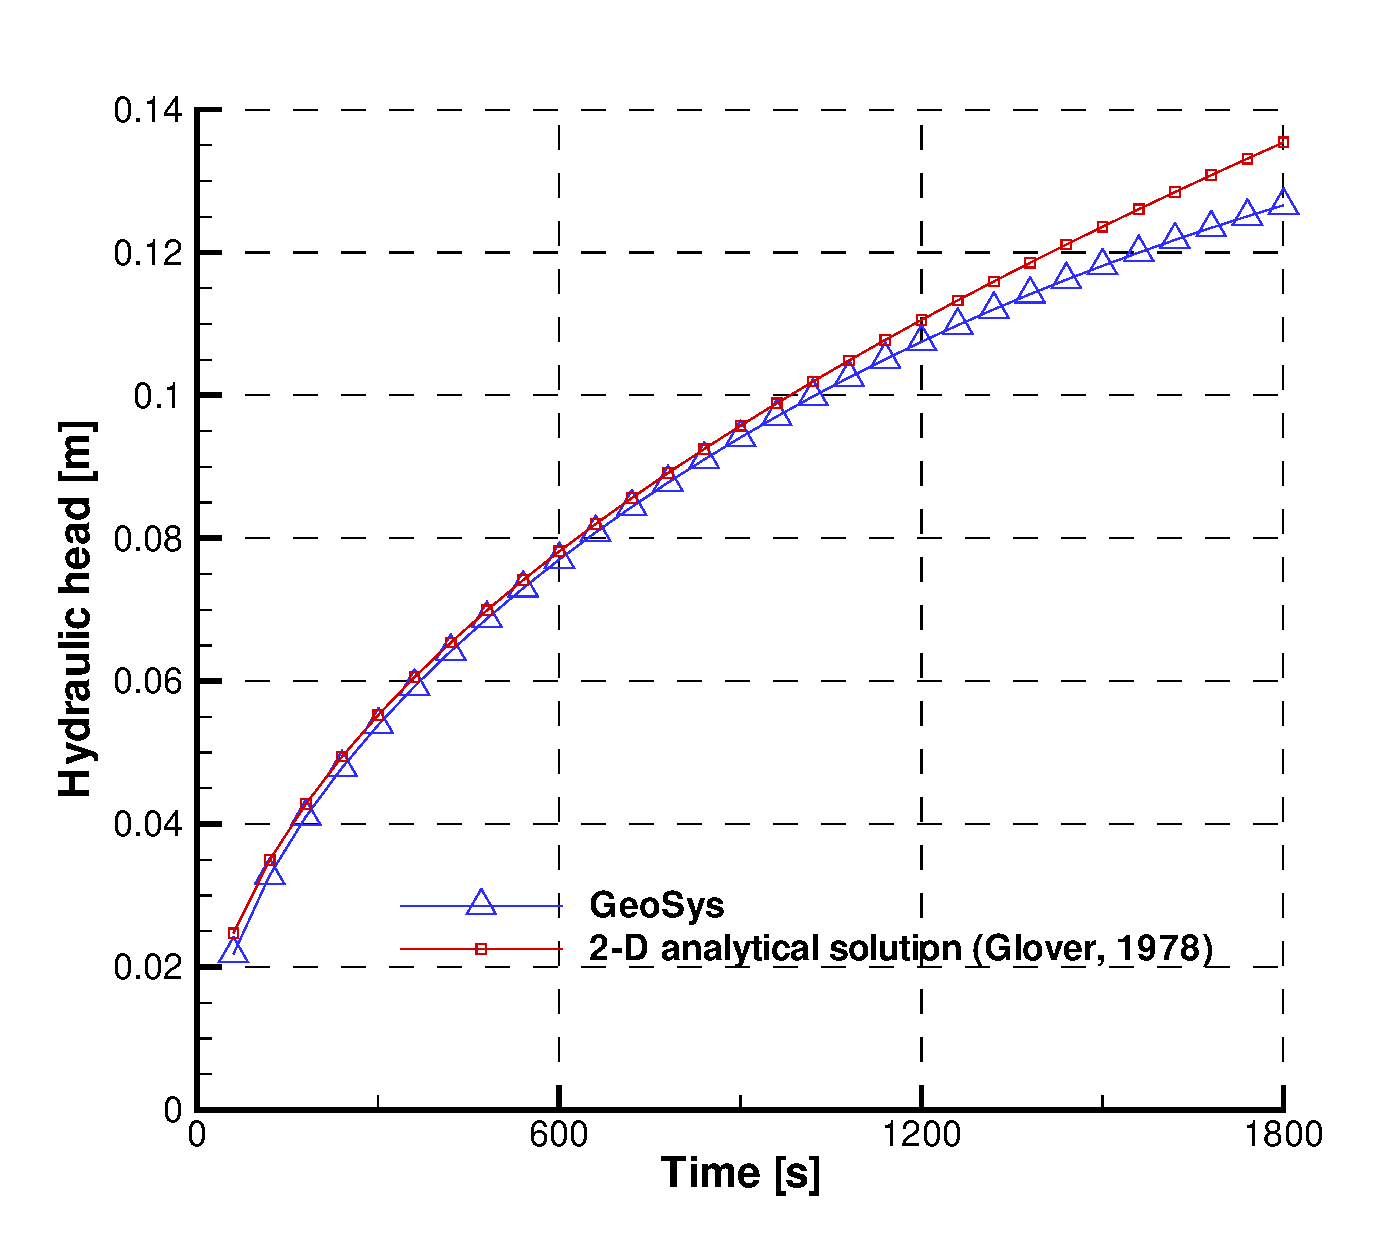
\includegraphics[width=0.6\columnwidth] {H_GW/figures/riv1_quad_point.eps}
\caption{Results with quadratic elements and analytical solution for confined aquifer below uniform and steady channel}
 \label{GW_Results_ChannelPercolation_quad}
\end{figure}
%
\begin{figure} [htb!]
 \centering
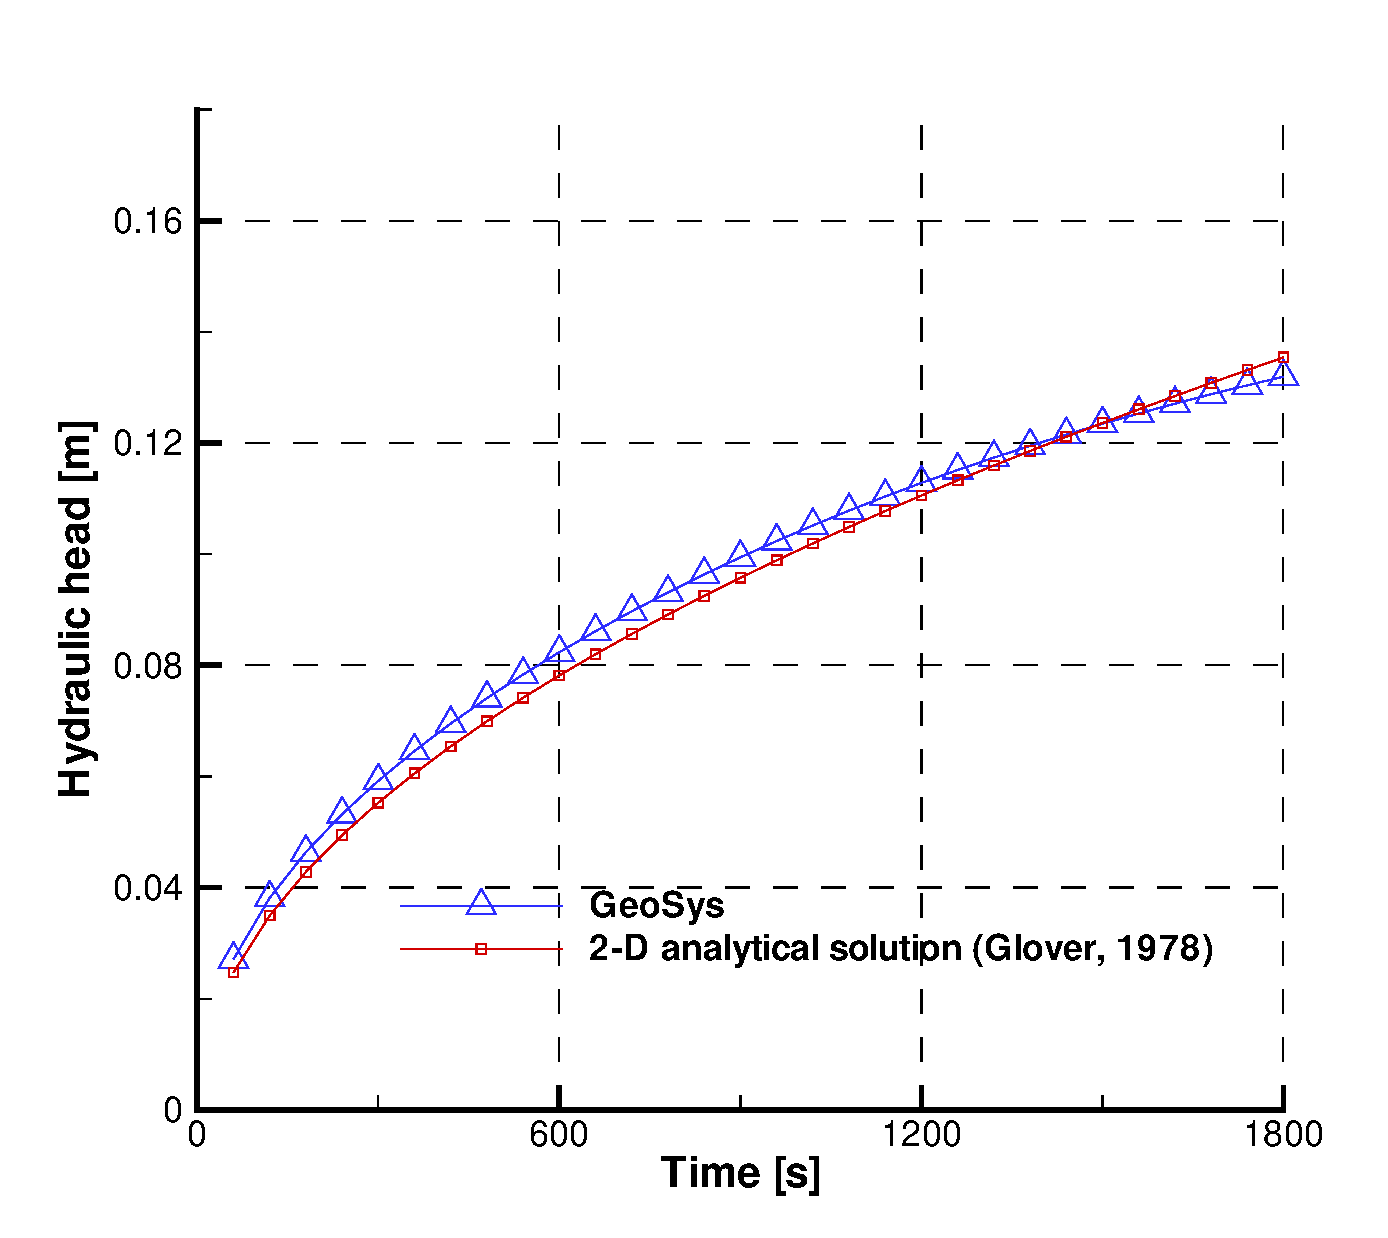
\includegraphics[width=0.6\columnwidth] {H_GW/figures/riv1_hex_point.eps}
\caption{Results with hexahedral and prismatic elements compared with the analytical solution for confined aquifer below uniform and steady channel}
 \label{GW_Results_ChannelPercolation_hex}
\end{figure}
%
\subsubsection*{Benchmark deposit}
%
\begin{tabular}{|l|l|l|}
  \hline
  Benchmark & Problem type & Path in benchmark deposit \\
  \hline
  \emph{riv1\_quad} & H & benchmarks\verb \GROUNDWATER_FLOW\ \\
  \emph{riv1\_pris} & H & benchmarks\verb \GROUNDWATER_FLOW\ \\
  \emph{riv1\_hex} & H & benchmarks\verb \GROUNDWATER_FLOW\ \\
 \hline
\end{tabular}
%
%--------------------------------------------------------------------------------------------------------------------------
%
\subsection{Channel sink term}
%
\subsubsection*{Problem definition}
%

For this example the channel of the previous examples (Sec.~\ref{sec:Groundwater_confined_channelSource}) is located such that flow from the aquifer to the channel takes place. Therefore, the source term represents a steady and uniform rectangular channel located in the aquifer. The setup is shown in Fig.~\ref{GW_riv1_domain}. The simulation time is $30min$.


\subsubsection*{Initial and boundary conditions}
%
Initial groundwater head is $0m$. The channel source term is the boundary condition at one side, at the opposite boundary the head is $0$. At the other boundaries no-flow is imposed.
\subsubsection*{Material properties}
%
The domain is discretization with $24\times 12$ quadrants. The time step size is $1 min$.
Simulation parameters for the aquifer and the channel source term are given in Tab.~\ref{GW_ChannelPercolation}.
%
\begin{table}[H]
 \centering
 \caption{Parameters for the channel sink term example}
 \centering \label{GW_ChannelPercolation}
 \begin{tabular}{llll}
 \hline\hline\noalign{\smallskip}
 {\bf Parameter} & {\bf Symbol} & {\bf Setting} & {\bf Unit} \\ \hline
 {\bf Aquifer} & & & \\
 Storage & $S$ & $0.2$ & $-$ \\
 Specific storage & $S_s$ & $0.2$ & $1/m$ \\
 Viscosity  & $\mu$ & $1\times 10^{-3}$ & $Pa\cdot s$\\
 Thickness & $L$ & $1$ & $m$ \\ \hline
 {\bf Channel source term} & & & \\
 Head & $h^{sur}$ & $-0.5$ & $m$ \\
 Bed top location& $z^{sur}$ & $-0.7$ & $m$ \\
 Width & $B$ & $59.6$ & $m$ \\
 Bed conductivity & $K_{\Lambda}$ & $1\times 10^{-6}$ & $m/s$ \\
 Bed thickness & $a$ & $0.3$ & $m$ \\
 \noalign{\smallskip}\hline\hline
 \end{tabular}
\end{table}
%
\subsubsection*{Results}
%
Simulation results are shown in Fig.~\ref{GW_Results_ChannelSink}.
%
\begin{figure} [htb!]
 \centering
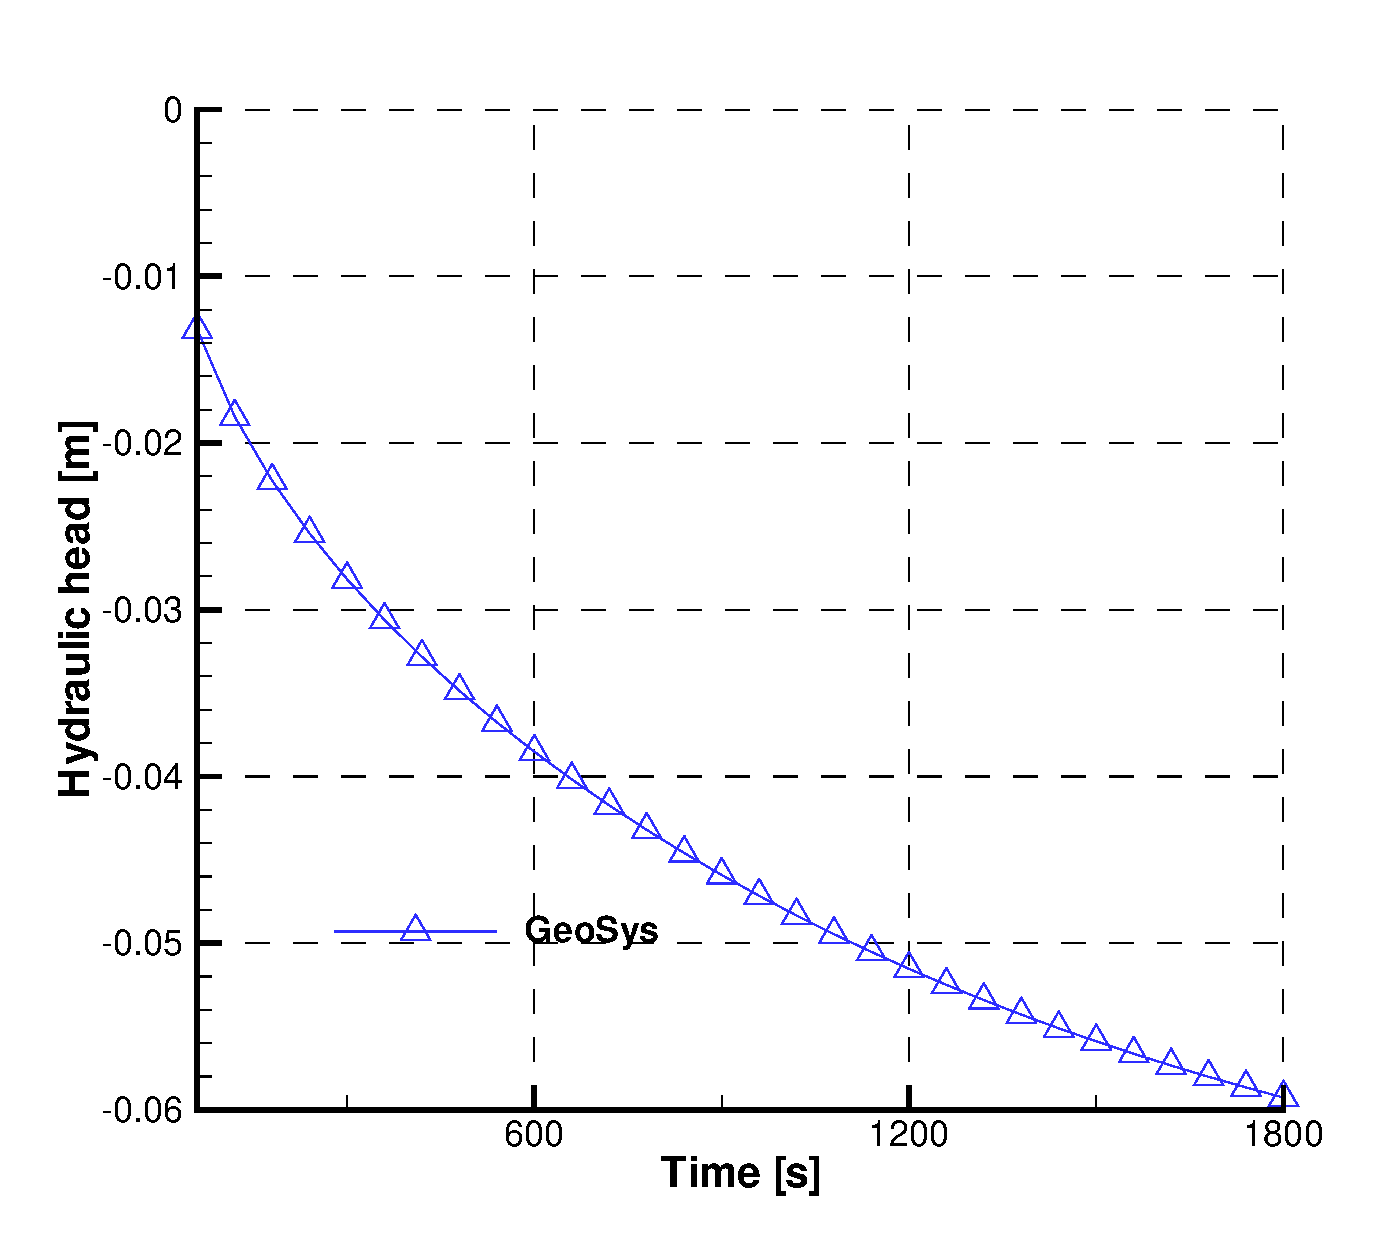
\includegraphics[width=0.6\columnwidth] {H_GW/figures/riv2_hex_point.eps}
\caption{Results by GeoSys for confined aquifer with a constant channel sink term}
 \label{GW_Results_ChannelSink}
\end{figure}
%
\subsubsection*{Benchmark deposit}
%
\begin{tabular}{|l|l|l|}
  \hline
  Benchmark & Problem type & Path in benchmark deposit \\
  \hline
  \emph{riv2\_hex} & H & benchmarks\verb \GROUNDWATER_FLOW\ \\
  \hline
\end{tabular}
%
%--------------------------------------------------------------------------------------------------------------------------
%
\subsection{Theis' Problem}
%
\subsubsection*{Problem definition}
%
Theis' problem examines the transient lowering of the water table induced by a pumping well. Theis' fundamental insight was to recognize that Darcy's law is analogous to the law of the flow of heat by conduction, hydraulic pressure being analogous to temperature, pressure-gradient to thermal gradient.
%
\subsubsection*{Assumptions}
%
\textit{Aquifer:} confined, infinite areal extend, homogeneous, isotropic, uniform thickness, horizontal piezometric surface;\\
\textit{Well:} constant discharge rate, well penetrates the entire thickness, well storage effects can be neglected.\\
%
\subsubsection*{Analytical solution}
The analytical solution of the drawdown as a function of time and distance is expressed by equation ~\ref{theis}:
%
\begin{eqnarray}
h_0 - h(t,x,y) = \frac{Q}{4\pi T}W(u)
\label{theis}
\end{eqnarray}
%
\begin{eqnarray}
u = \frac{(x^{2}+y^{2})S}{4Tt}
\label{theis_u}
\end{eqnarray}
%
where:\\ \\
%
\begin{tabular}{|l|l|l|}
  \hline
  symbol & property & unit \\
  \hline
  \ $h_0$ & constant initial hydraulic head & L \\
  \hline
  \ Q & constant discharge rate & $L^{3}T^{-1}$ \\
  \hline
  \ T & aquifer transmissivity & $L^{2}T^{-1}$\\
  \hline
  \ t & time & T\\
  \hline
  \ x,y & the coordinate at any point & L\\
  \hline
  \ S & aquifer storage & -\\
  \hline
\end{tabular}
%

\subsubsection*{Initial and boundary conditions}
%
\begin{tabular}{|l|l|}
  \hline
  Parameters/conditions & OpenGeoSys \\
  \hline
  Initial conditions & h(0,r)=0  \\
  \hline
  Sink, well pumping rate & $Q=1.22329\times 10^{3} m^{3} d^{-1}$  \\
  \hline
  Boundary conditions & h(t,304.8m)=0  \\
  \hline
   flow materials&   \\
  \hline
    -Hydraulic conductivity & $9.2903\times 10^{-4}m s^{-1}$  \\
  \hline
    -storage coefficient & S=0.001   \\
  \hline
    -storage compressibility & 0  \\
  \hline
    -wellbore radius & 0.3048m  \\
  \hline
\end{tabular}
%
\begin{figure} [htb!]
 \centering
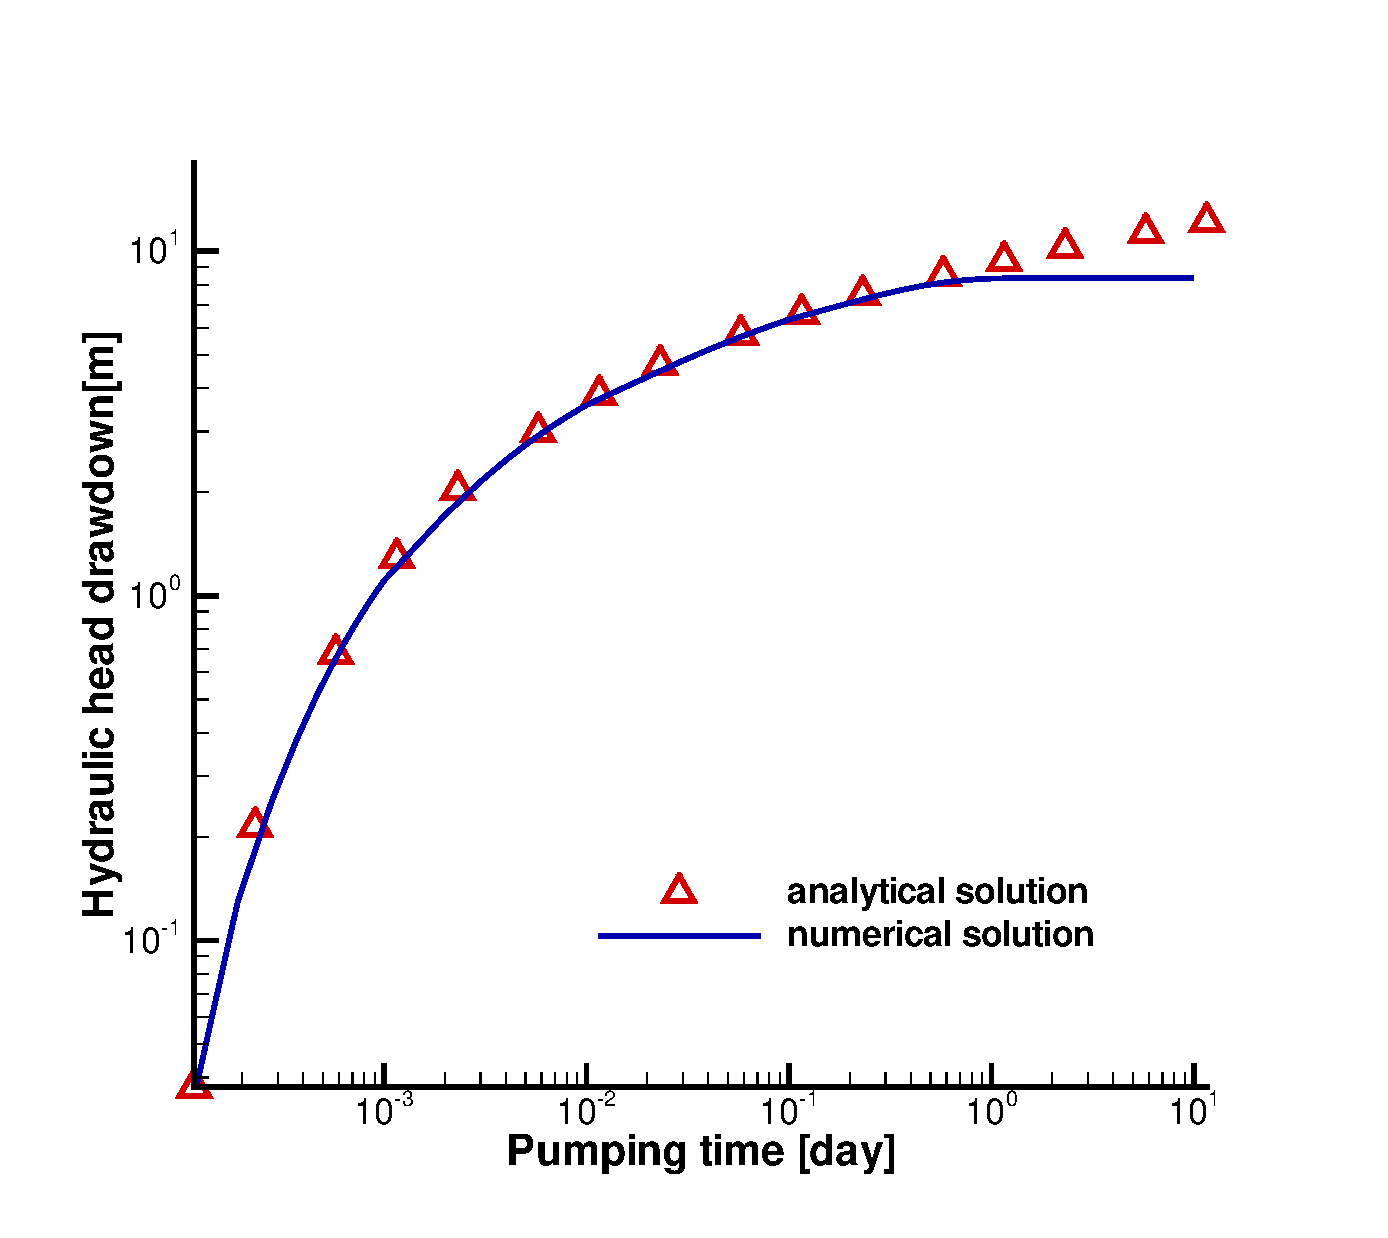
\includegraphics[width=0.7\columnwidth] {H_GW/figures/Theis1.eps}
\caption{Calculated drawdowns at a distance of 9.639m from the well.}
 \label{Theis1}
\end{figure}
%
%
\subsubsection*{Results}
Fig.~\ref{Theis1} shows the comparison of analytically and numerically caculated drawdown of hydraulic head versus time at the distance of r = 9.639 m from the well.
\subsubsection*{Benchmark deposit}
%
\begin{tabular}{|l|l|l|}
  \hline
  Benchmark & Problem type & Path in benchmark deposit \\
  \hline
  \emph{h\_quad\_axisym} & H & benchmarks\verb \H\Theis_1D\ \\
  \hline
\end{tabular}

%
\begin{figure} [htb!]
 \centering
 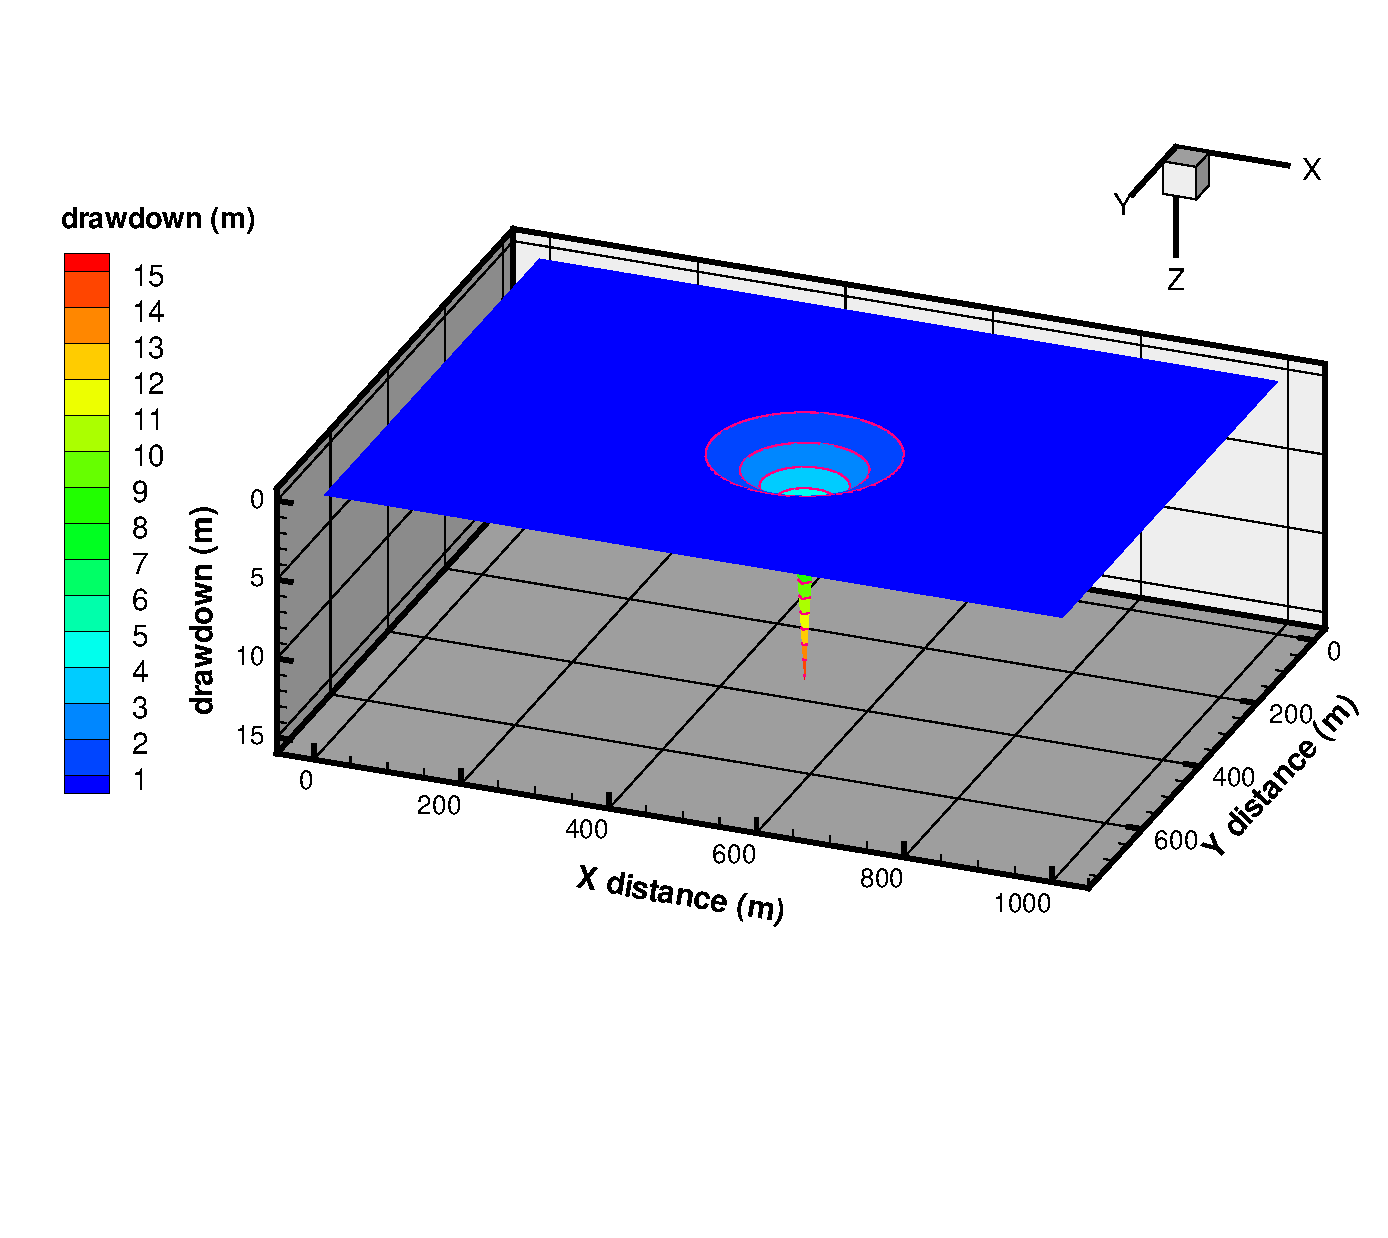
\includegraphics[width=0.9\columnwidth] {H_GW/figures/theis2.eps}
 \caption{Cone of depression at the end of the simulation.}
 \label{theis2}
\end{figure}
%
%
\subsubsection*{2D application}
%
The 2D application is solved in the following situation:\\
\\
%
\begin{tabular}{|l|l|l||l|}
  \hline
  parameters& description & values & unit \\
  \hline
  Q & discharge rate & 1000  & $m^{3}d^{-1}$  \\
  S & specific storage & $1.0\times 10^{-5}$ & $m^{-1}$ \\
  T & transmissivity & 1000 &  $m^{2}d^{-1}$ \\
  B & thickness of aquifer & 20 & m \\
  \hline
\end{tabular}
\\
\\
The aquifer horizontal domain size is 1000m $\times$ 750 m with the pumping well at the location coordinate (500,375).The discretization of space is 10m $\times$ 10m grid. The simulation time is 0.00175 day and the time step is 1.036 sec. The boundary condition is 0.0 drawdown.
The cone of depression induced by the pumping well at the end of the simulation is plotted in Fig.~\ref{theis2}.
\subsubsection*{Benchmark deposit}
%
\begin{tabular}{|l|l|l|}
  \hline
  Benchmark & Problem type & Path in benchmark deposit \\
  \hline
  \emph{h\_quad\_axisym} & H & benchmarks\verb \H\Theis_2D\ \\
  \hline
\end{tabular}
%

%----------------------------------------------------------------------------------------------------------------------------------

\section{Time variant flow}

This benchmark is set up to test the implementation of time variant boundary conditions for the \texttt{GROUNDWATER\_FLOW} process. These boundary conditions allow to simulate flow and transport in a flow field, which changes gradient and direction according to user specified functions.

The setup of the model domain is depicted in Figure \ref{time_variant_flow_setup}. The model geometry is designed by 4 corner nodes (gli nodes 0 through 3), which are connected along the model edges by one polyline each. To induce a time variant flow field, time functions are generated externally and are connected to the corner gli nodes. The polyline names and location and the names of the time functions are shown in Figure \ref{time_variant_flow_setup}.

To connect the time functions with the boundary condition, the boundary condition has to be specified along a polyline. The distribution type is \texttt{LINEAR} followed by the number of nodes of the polyline (2) and then by two lines specifying the gli node number, the value at this node and the name of the time function. The value of the time function at the corresponding time is then multiplied by the specified value at the nodes and interpolated to all mesh nodes found along the polyline. This is performed in each timestep. In the case shown here, this was applied for all four boundary condition polylines along the four model area sides.

\small
\begin{verbatim}
#BOUNDARY_CONDITION
 $PCS_TYPE
  GROUNDWATER_FLOW
 $PRIMARY_VARIABLE
  HEAD
 $GEO_TYPE
  POLYLINE BCLEFT
 $DIS_TYPE
  LINEAR 2
   0 1.0 BC_left_low
   3 1.0 BC_left_high
   \end{verbatim}
\normalsize

The model area is 184 m in x direction and 64 m in y direction. Boundary conditions are placed along all four sides of the model area. Hydraulic conductivity is 0.00215 m s$^{-1}$, the storage coefficient is set to 0. Initial conditions are a head of 2.0239 m everywhere.

The benchmark tests at the same time the application of a heterogeneous distribution of the hydraulic conductivity. This is achieved by setting in the *.mmp file:
\small
\begin{verbatim}
 $PERMEABILITY_TENSOR
  ISOTROPIC 1.0
 $PERMEABILITY_DISTRIBUTION
  2d_het_a_kfhet
\end{verbatim}
\normalsize

The file \texttt{2d\_het\_a\_kfhet} contains the heterogeneous distribution of the hydraulic conductivity, and is generated using an geostatistical simulator. The file contains information on the \texttt{\$MSH\_TYPE}, the \texttt{\$MMP\_TYPE} and specifies options for the interpolation of the values onto the elements of the specified mesh (\texttt{\$DIS\_TYPE}). Under the keyword \texttt{\$DATA} the actual values are specified as x - y - parameter values, where parameter is the hydraulic conductivity. The end of the data set is marked using the keyword \texttt{\#STOP}.

\small
\begin{verbatim}
#MEDIUM_PROPERTIES_DISTRIBUTED	
; Specify mesh, for which data is read
$MSH_TYPE
  GROUNDWATER_FLOW
$MMP_TYPE
 PERMEABILITY
; give interpolation option: NEAREST_VALUE or GEOMETRIC_MEAN
$DIS_TYPE
 NEAREST_VALUE
$CONVERSION_FACTOR
 1.0
; X, Y, Z, nof field values			
$DATA
33.00  35.00 0 1.0903602235e-004
25.00  37.00 0 8.4356781197e-005
125.00  21.00 0 5.7274327695e-005
...
\end{verbatim}
\normalsize




The result of the simulation is shown in Figures \ref{time_variant_heads_results} in top view. The full contours show the piezometric head isolines after the first five time steps, the black and red lines show head isolines from a succession of time steps. It can be seen, that the flow field is turned and directed upwards (black isolines) and back again (red isolines) during the simulation. Figure \ref{time_variant_heads_observationwell} shows the time variant head in an observation well at x=20 m and y=28 m. The rise and fall of the piezometric head due to the time variant flow field can be clearly seen, as well as the initial jump from the initial head to the time variant head.

\begin{figure}[htbp]
\centering
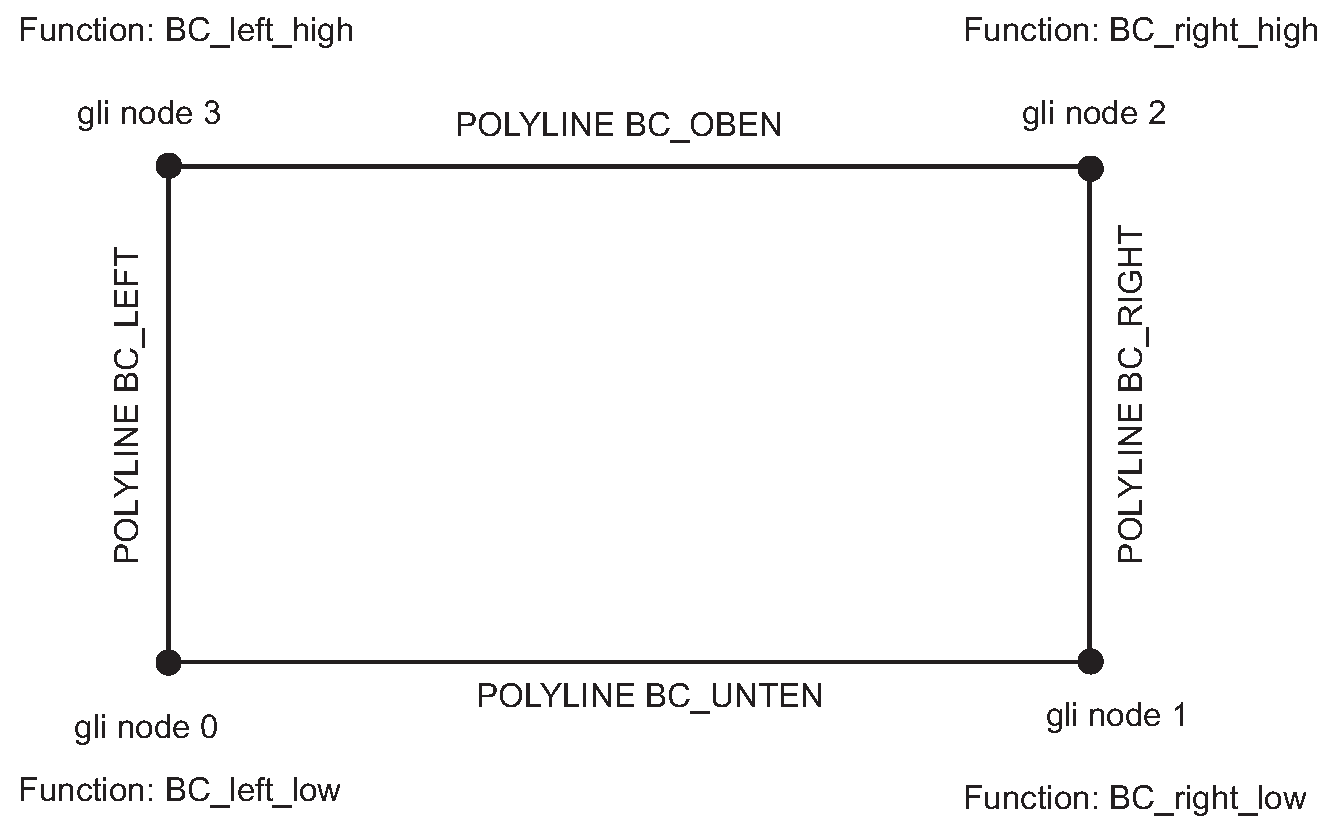
\includegraphics[width=0.6\textwidth]{H_GW/figures/time_variant_flow_setup.eps}
\caption{Model setup for the time variant flow}
\label{time_variant_flow_setup}
\end{figure}

\begin{figure}[htbp]
\centering
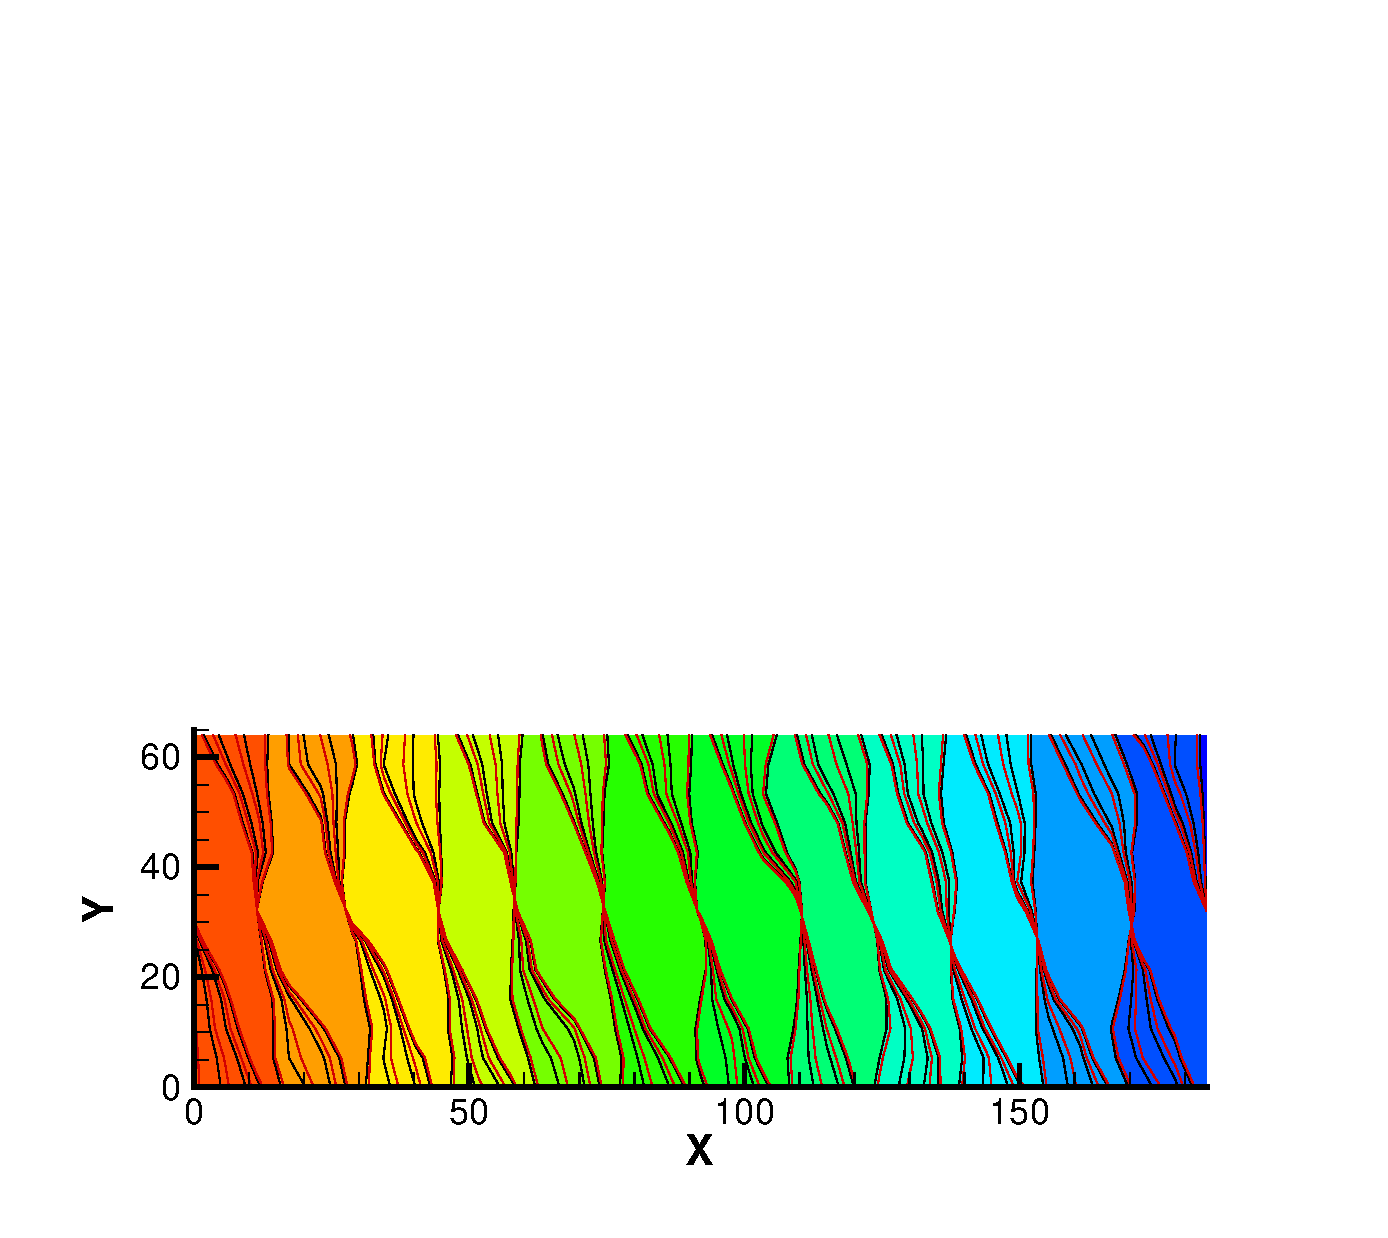
\includegraphics[width=0.75\textwidth]{H_GW/figures/time_variant_heads_results.eps}
\caption{Model results for the time variant heads in top view}
\label{time_variant_heads_results}
\end{figure}

\begin{figure}[htbp]
\centering
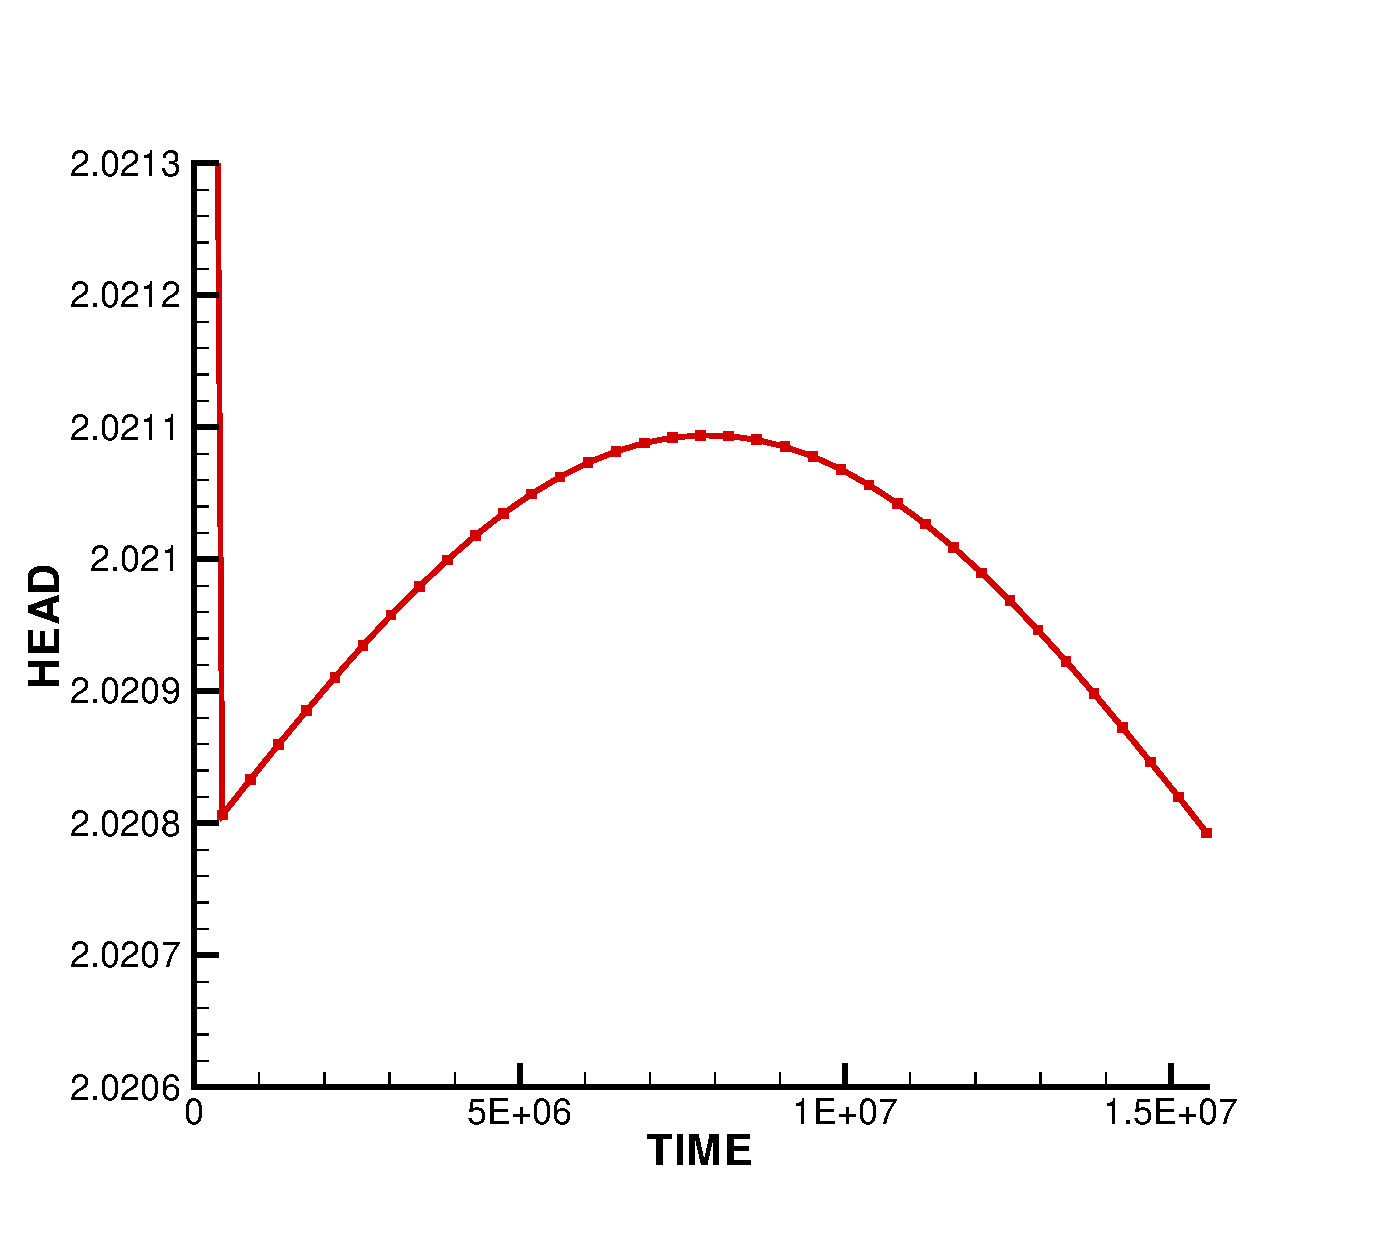
\includegraphics[width=0.4\textwidth]{H_GW/figures/time_variant_heads_observationwell.eps}
\caption{Model results at one observation well}
\label{time_variant_heads_observationwell}
\end{figure}

\begin{table}[htbp]
\centering
\begin{tabular}{|l|l|l|}
\hline
Benchmark & Type & Path \\
\hline
\texttt{transient\_flow}& H &  benchmarks$\backslash$GROUNDWATER\_FLOW$\backslash$transient\_flow  \\			
\hline
\end{tabular}
\end{table}


%--------------------------------------------------------------------------------------------------------------------------
%
\section{Unconfined aquifer}
\label{sec:Groundwater_unconfined}
%
\subsection{Steady state case}
%
\subsubsection*{Problem definition}
%
In these examples the aquifer consists of a small strip with the size of $100m \times 2m$ (see Fig.~\ref{GW_Results_uc}). At both ends the head is fixed and constant recharge is imposed on the whole domain which leads to steady state flow. This setting allows comparison with an analytical solution.
%\emph{uc\_quad}, \emph{uc\_tri} solve the two-dimensional Eqn.~\ref{eqn:GW_unconfinedGoverning}  for unconfined auifer and \emph{uc\_pris} solves the three-dimensional groundwater Eqn.\ref{eqn:GW_Governing}.
%
\subsubsection*{Initial and boundary conditions}
%
Initial groundwater head is $0m$. At one end of the strip the head is $1$ at the other $5$. At the top a source term of $1.0\times 10^{-8} m/s$ and at the remaining parts no-flow is imposed.
\subsubsection*{Material properties}
%
For the spatial discretization $100$ equal quadrants and $410$ triangles or prisms are used. In latter case the three-dimensional groundwater Eqn.~\ref{eqn:GW_unconfinedGoverning} is solved with elements adapting to the water height. One time step with the size of $100 s$ is used. The specific storage $S_s = 0 m^{-1}$ or specific yield $S_y = 0$ and a permeability $\kappa$ of $1\times 10^{-9} m^2$ is used.
%
\subsubsection*{Results}
%
Comparison of simulation results for prisms and analytical solution is shown in Fig.~\ref{GW_Results_uc}.
%
\begin{figure} [htb!]
 \centering
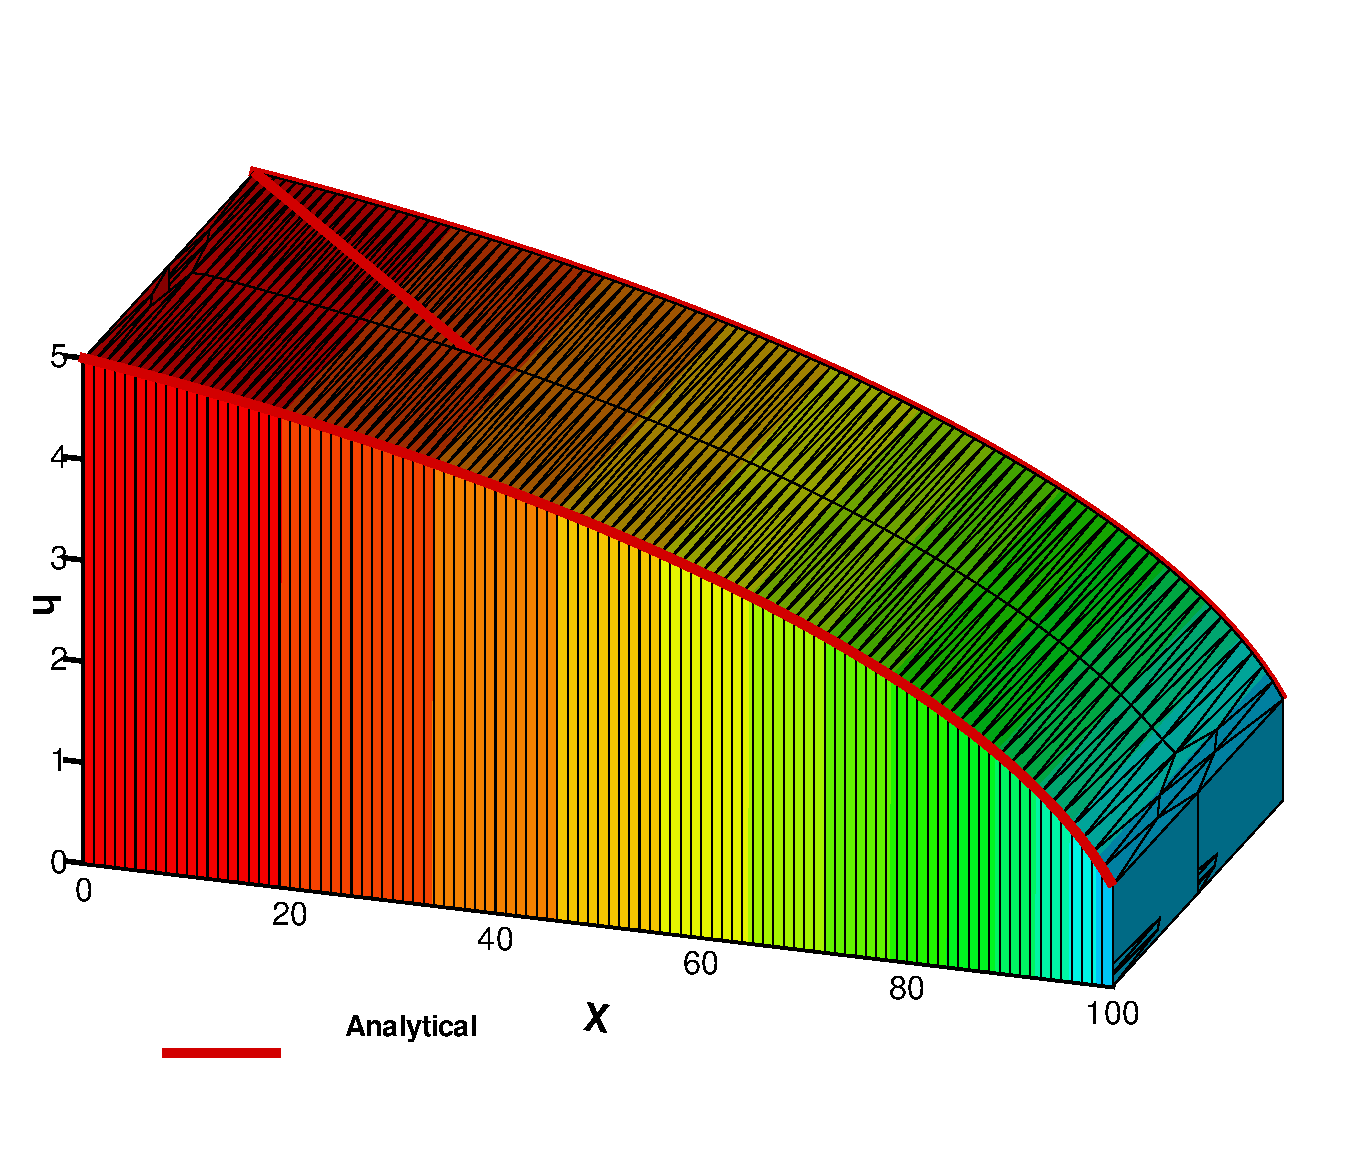
\includegraphics[width=0.7\columnwidth] {H_GW/figures/uc_pris.eps}
\caption{Results of unconfined aquifer benchmark example by GeoSys with prisms}
 \label{GW_Results_uc}
\end{figure}
%
\subsubsection*{Benchmark deposit}
%
\begin{tabular}{|l|l|l|}
  \hline
  Benchmark & Problem type & Path in benchmark deposit \\
  \hline
  \emph{uc\_quad} & H & benchmarks\verb \GROUNDWATER_FLOW\ \\
  \emph{uc\_tri} & H & benchmarks\verb \GROUNDWATER_FLOW\ \\
  \emph{uc\_pris} & H & benchmarks\verb \GROUNDWATER_FLOW\ \\
  \hline
\end{tabular}

%
%--------------------------------------------------------------------------------------------------------------------------
% 
\chapter{Fluid property functions}
\label{chap-FP}
\section{Theory of thermodynamic and transport properties}

%% \newfont{\tensy}{cmsy10}
%% \newcommand{\chemical}[1]{{$\fontdiment16\tensy=3.0pt\fontdiment17\tensy=3.0pt \mathrm{#1}$}}


%\subsection{Thermodynamic properties}

\subsection{Density} \label{eos-density}

In subterranean oil and gas reservoirs, properties of gases and liquids strongly depend from environmental pressure and temperature conditions. Equations of state (EOS) may be used to describe the relationship of volume, pressure and temperature of a real fluid. The knowledge of a fluids volume or its density is essential to estimate further thermodynamic properties. The first EOS for real gases, which was based on the ideal gas law, was presented by Johannes Diderik \textsc{van der Waals} in 1873 \cite{VanWaa:73}. In 1910 he received the Nobel prize for the development of the equation

\begin{equation}
p=\frac{RT}{V_m-b}-\frac{a}{V^2_m}
\label{eq-van-der-waals}
\end{equation}

where $p$ is the pressure, $R$ is the gas constant, $T$ is the temperature, $V_m$ is the molare volume and $a$ and $b$ are correcting parameters. 

%For the development of this equation \eqref{eq-van-der-waals}, \textsc{van der Waals} received the Nobel prize in 1910.
%
%\begin{equation}
%P=\frac{RT}{v-b}-\frac{a}{v^2}
%\label{eq-van-der-waals}
%\end{equation}

%In the current version of GeoSys\,(4.10.0), three different Equations of state are implemented. 
%\begin{itemize}
%	\item \textsc{Redlich-Kwong}, 1949 \cite{RedKwo:49}
%	\item \textsc{Peng-Robinson}, 1975 \cite{PenRob:75}
%	\item Fundamental equations, see \cite{SpaWag:96},\cite{PruWag:95},\cite{BueWag:06},  \cite{SpaLem:00}, and \cite{SetWag:91}
%\end{itemize}

Following three different EOS will be described, which are implemented in version GeoSys\,(4.10.00), based on the \textsc{van der Waals}-equation~\eqref{eq-van-der-waals}. % JG Satzumstellung

\paragraph{Redlich-Kwong equation of state (RKEOS)}
The Equation of \textsc{Redlich} and \textsc{Kwong} from 1949 \eqref{eq-rkeos1} represents just a little improvement of the van der Waals equation \cite{RedKwo:49}. It is given as 														

\begin{equation}
p=\frac{RT}{V_m-b}-\frac{a}{T^{0.5}\,V_m\,(V_m+b)}.
\label{eq-rkeos1}
\end{equation}

Its results are satisfactory only for temperatures above the critical point (see Tab.~\ref{tab-eos2}). 

\begin{table}[H]
  \caption{\label{tab-eos2}Fluid properties used in equations of state, where $\omega$ is the acentric factor, $T_c$ and $p_c$ are temperature und pressure at the critical point and $R$ ist the gas constant.}
  \begin{center}
\begin{tabular}{lrrrr}
\toprule
  substance 		& $\omega$ [-]  & $T_c$ [K] & $p_c$ [MPa] & $R$ [J/kg/K]\\
\midrule
  Carbon dioxide & 0.239  			& 304.13 & 7.38 		& 188.9\\
  Ethane         & 0.099  			& 305.32	& 4.87 		& 276.5\\
  Methane        & 0.011  			& 190.56 & 4.60 		& 518.3\\
  Water          & 0.344  			& 647.10 & 22.06 		& 461.5\\
\bottomrule
\end{tabular}
\end{center}
\end{table}

Equation \eqref{eq-rkeos1} can be recasted as a cubic equation in terms of volume

\begin{equation}
V_m^3-\frac{RT}{p}V_m^2-\left(\frac{RTb}{p}-\frac{a}{T^{0.5}p}+b^2\right)V_m-\frac{ab}{T^{0.5}p}=0.
\label{eq-rkeos2}
\end{equation}
              
This equation yields to one or three real roots depending on the number of phases in the system. In the two-phase region, the largest positive root represents the molar volume of the gas phase while the smallest root correspondes to the volume of the liquid phase. The correcting terms $a$ and $b$ are given as
													
\begin{equation}
a=0.4275\,\frac{R^2 T_c^{2.5}}{p_c}
\label{eq-rkeos_a}
\end{equation}

and

\begin{equation}
b= 0.0866\,\frac{RT_c}{p_c}
\label{eq-rkeos_b}
\end{equation}

where $T_c$ and $p_c$ are Temperature and pressure at the critical point (see Tab.~\ref{tab-eos2}). Figs.~\ref{fig-eos-dens-ch4-co2} and \ref{fig-eos-dens-h2o-n2} show the results of the RKEOS for several substances at four different temperatures in comparison to other equations of state.


%\begin{figure}
%\begin{minipage}{0.49\textwidth}
%\centering
%\includegraphics[width=1\textwidth]{FLUID_PROPERTIES/figures/dens-ch4.eps}
%\caption[bild1]{Density of $\mathrm{CH_4}$ derived by different equations of state}
%\label{fig-eos-dens-ch4}
%\end{minipage}
%%
%\hspace{0.02\textwidth
%}
%\begin{minipage}{0.49\textwidth}
%\centering
%\includegraphics[width=1\textwidth]{FLUID_PROPERTIES/figures/dens-co2.eps}
%\caption[bild2]{Density of $\mathrm{CO_2}$ derived by different equations of state}
%\label{fig-eos-dens-co2}
%\end{minipage}
%\end{figure}


\begin{figure}
\subfigure[]{\label{fig-eos-dens-ch4}\includegraphics[width=0.5\textwidth]{FLUID_PROPERTIES/figures/dens-ch4.eps}}
\hfill
\subfigure[]{\label{fig-eos-dens-co2}\includegraphics[width=0.5\textwidth]{FLUID_PROPERTIES/figures/dens-co2.eps}}
\caption[]{\label{fig-eos-dens-ch4-co2}Density of \ch4~\subref{fig-eos-dens-ch4} and \co2~\subref{fig-eos-dens-co2} derived by different EOS. There stand 
\setlength{\unitlength}{1ex}
\begin{picture}(5,1)
\thicklines \put(0,0.5){\line(1,0){5}}
\end{picture}
for the \textsc{Helmholtz} Free Energy,
\begin{picture}(5,1)
\thicklines \multiput(0,0.5)(2,0){3}{\line(1,0){1}}
\end{picture}
for the PREOS and
\begin{picture}(5,1)
\thicklines \multiput(0,0.5)(2,0){3}{\line(1,0){1}}\multiput(1.4,0.5)(2,0){2}{\line(1,0){0.25}}
\end{picture}
for the RKEOS. The colours refer to different temperatures (\textcolor{blue}{blue} - $\unit[280]{K}$, \textcolor{violet}{violet} - $\unit[320]{K}$, \textcolor{purple}{pink} - $\unit[400]{K}$, \textcolor{red}{red} - $\unit[680]{K}$).}
\end{figure}




%\begin{figure}
%\begin{minipage}{0.49\textwidth}
%\centering
%\includegraphics[width=1\textwidth]{FLUID_PROPERTIES/figures/dens-h2o.eps}
%\caption[bild1]{Density of $\mathrm{H_2O}$ derived by different equations of state}
%\label{fig-eos-dens-h2o}
%\end{minipage}
%%
%\hspace{0.02\textwidth
%}
%\begin{minipage}{0.49\textwidth}
%\centering
%\includegraphics[width=1\textwidth]{FLUID_PROPERTIES/figures/dens-n2.eps}
%\caption[bild2]{Density of $\mathrm{N_2}$ derived by different equations of state}
%\label{fig-eos-dens-n2}
%\end{minipage}
%\end{figure}


\begin{figure}
\subfigure[]{\label{fig-eos-dens-h2o}\includegraphics[width=0.5\textwidth]{FLUID_PROPERTIES/figures/dens-h2o.eps}}
\hfill
\subfigure[]{\label{fig-eos-dens-n2}\includegraphics[width=0.5\textwidth]{FLUID_PROPERTIES/figures/dens-n2.eps}}
\caption[]{\label{fig-eos-dens-h2o-n2}Density of \h2o~\subref{fig-eos-dens-h2o} and \n2~\subref{fig-eos-dens-n2} derived by different EOS. There stand 
\setlength{\unitlength}{1ex}
\begin{picture}(5,1)
\thicklines \put(0,0.5){\line(1,0){5}}
\end{picture}
for the \textsc{Helmholtz} Free Energy,
\begin{picture}(5,1)
\thicklines \multiput(0,0.5)(2,0){3}{\line(1,0){1}}
\end{picture}
for the PREOS and
\begin{picture}(5,1)
\thicklines \multiput(0,0.5)(2,0){3}{\line(1,0){1}}\multiput(1.4,0.5)(2,0){2}{\line(1,0){0.25}}
\end{picture}
for the RKEOS. The colours refer to different temperatures (\textcolor{blue}{blue} - $\unit[280]{K}$, \textcolor{violet}{violet} - $\unit[320]{K}$, \textcolor{purple}{pink} - $\unit[400]{K}$, \textcolor{red}{red} - $\unit[680]{K}$).}
\end{figure}



\paragraph{Peng-Robinson equation of state (PREOS)}
D.\,Y.\,\textsc{Peng} and D.\,B.\,\textsc{Robinson} presented an improvement of the RKEOS in 1975 \cite{PenRob:75}. The proposed equation is also a two-constant van der Waals-Type equation and combines simplicity and accuracy. The PREOS is very simple to solve and gives satisfying results within the whole fluid redion of a gas. It is given in the form

\begin{equation}
p=\frac{RT}{V_m-b}-\frac{a(T_c)\cdot \alpha (T_r,\omega)}{V_m^2+2\cdot bV_m-b^2}
\label{eq-preos1}
\end{equation}

where $a$ and $b$ are correcting terms. They can be derived by %\eqref{eq-preosa} and \eqref{eq-preosb} 

\begin{equation} 
a(T_c) = 0.45724\,\frac{R^2T_{c}^{2}}{p_c}
\label{eq-preosa}
\end{equation}

and

\begin{equation} 
b(T_c) = 0.07780\,\frac{RT_c}{p_c}
\label{eq-preosb}
\end{equation}

for the particular fluids under specification of pressure and temperature at the critical point.
Parameter $\alpha(T_r,\omega)$ is a dimensionless function of reduced temperature $T_r$ and acentric factor $\omega$. It is given as

\begin{equation} 
\alpha = \left( 1+ \left(0.37464 + 1.54226\,\omega - 0.26992\,\omega^2\right)\left(1-T_r^{0.5}\right)\right)^2
\label{eq-preosalpha1}
\end{equation}

for $\omega\leq{0.49}$ and

\begin{equation} 
\alpha = \left( 1+ \left(0.379642 + \left(1.48503-\left(1.164423-1.016666\,\omega\right)\omega\right)\omega\right)\left(1-T_r^{0.5}\right)\right)^2
\label{eq-preosalpha2}
\end{equation}

for $\omega > 0.49$. 

Tab.~\ref{tab-eos2} shows acentric factors and critical parameters for different real gases. The resulting density distribution of the 
PREOS is shown in Figs.~\ref{fig-eos-dens-ch4-co2} and \ref{fig-eos-dens-h2o-n2} at four different temperatures. 

%-----> JG: Vorschlag fr diesen Abschnitt s.u.

%\paragraph {Fundamental equations}				
%For highly precise results it is necessary to adapt fundamental equations based on the free energy, see \eqref{eq-fhe1}. Many authors used this approach to develop EOS for different substances, e.\,g.\,:
%
%\begin{itemize}
%\item \textsc{Span\&Wagner} \cite{SpaWag:96}, \cite{Spa:93}, \cite{SpaLem:00} for carbon dioxide and for nitrogen,
%\item \textsc{Pru\&Wagner} \cite{PruWag:95}, \cite{WagPru:02} for water,
%\item \textsc{Bcker\&Wagner} \cite{BueWag:06} for ethane and
%\item \textsc{Setzmann\&Wagner} \cite{SetWag:91} for methane.
%\end{itemize}
%
%Equation \eqref{eq-fhe1} shows \textsc{Helmholtz} free energy in dependence from density $\rho$ and temperature $T$ in its dimensionless shape, where $\phi^{o}$ is an ideal gas part and $\phi^{r}$ represents a residual part. 
%
%\begin{equation}
%\frac{f(\rho,T)}{RT}=\phi(\delta,\tau)=\phi^{o}(\delta,\tau)+\phi^{r}(\delta,\tau)
%\label{eq-fhe1}
%\end{equation}
%where $\delta=\rho/\rho_c$ and $\tau=T_c/T$\footnote{$\rho_c$ and $T_c$ are density and temperature at the critical point, see table \ref{tab-eos2}}
%The fundamental equation (\ref{eq-fhe1}) according to \textsc{Wagner} et al. (\cite{SpaWag:96},\cite{PruWag:95},\cite{BueWag:06}, and \cite{SetWag:91}) is one of the most precise EOS at present. The Equation and its derivatives can be used to describe all thermodynamic properties of a pure substance depending on density and temperature. So, it is necessary to solve the relationship between density, pressure, and temperature (eq. \ref{eq-fhe-dens}) iteratevly.
%
%\begin{equation}
%\frac{p(\delta,\tau)}{\rho RT}=1+\delta \frac{\partial \phi^r}{\partial \delta}
%\label{eq-fhe-dens}
%\end{equation}
%
%For water, the equation became international standard for the IAPWS since 1995. Certainly, the equation is complicated to solve and requires long computing time. Therefore, in the current version of Geosys, it is possible to choose between an iterative solving algorithm and an interpolation of density values out of a database. 
%


\paragraph {Fundamental equations}			
For highly precise results it is necessary to adapt fundamental equations based on the free energy. The \textsc{Helmholtz} free energy is given as

\begin{equation}
\frac{f(\rho,T)}{RT}=\phi(\delta,\tau)=\phi^{o}(\delta,\tau)+\phi^{r}(\delta,\tau)
\label{eq-fhe1}
\end{equation}
in dependence from density $\rho$ and temperature $T$ in its dimensionless form. These dimensionless parts are given as the terms $\delta=\rho/\rho_c$ and $\tau=T_c/T$, whereas $\rho_c$ and $T_c$ are density and temperature at the critical point (see Tab.~\ref{tab-eos2}).  The \textsc{Helmholtz} free energy provides relations between density, temperature and all thermodynamic properties of a fluid, which are expressed in the parameter $\phi^{o}$ as the ideal gas part and $\phi^{r}$ as the residual part. For their derivatives in the short forms like
$\phi^r_\delta$,\hspace{0.1cm} 
$\phi^r_{\delta\delta}$,\hspace{0.1cm} 
$\phi^r_\tau$,\hspace{0.1cm} 
$\phi^r_{\tau\tau}$,\hspace{0.1cm} 
$\phi^r_{\delta\tau}$,\hspace{0.1cm}
$\phi^o_\tau$,\hspace{0.1cm} 
$\phi^o_{\tau\tau}$
it is refered to \cite{SpaWag:96}.

Many authors used the approach of \textsc{Helmholtz} free energy to develop EOS for different substances, e.\,g.\,:

\begin{itemize}
\item \textsc{Span\&Wagner} \cite{SpaWag:96}, \cite{Spa:93}, \cite{SpaLem:00} for carbon dioxide and for nitrogen,
\item \textsc{Pruß\&Wagner} \cite{PruWag:95}, \cite{WagPru:02} for water,
\item \textsc{Bücker\&Wagner} \cite{BueWag:06} for ethane and
\item \textsc{Setzmann\&Wagner} \cite{SetWag:91} for methane.
\end{itemize}

The fundamental equation (\ref{eq-fhe1}) according to \textsc{Wagner} et al.\ (\cite{SpaWag:96},\cite{PruWag:95},\cite{BueWag:06}, and \cite{SetWag:91}) is one of the most precise EOS at present. The Equation and its derivatives can be used to describe all thermodynamic properties of a pure substance depending on density and temperature. So it is necessary to solve the relationship between density, pressure and temperature  iteratevly, as \eqref{eq-fhe-dens} shows

\begin{equation}
\frac{p(\delta,\tau)}{\rho RT}=1+\delta \frac{\partial \phi^r}{\partial \delta}.
\label{eq-fhe-dens}
\end{equation}

For water, the equation became international standard for the IAPWS\,\footnote{International Association for the Properties of Water and Steam} since 1995. Certainly, the equation is complicated to solve and requires long computing time. Therefore, in the version of GeoSys\,(4.10.00) it is possible to choose between an iterative solving algorithm 
and an interpolation of density values out of a database. 

The semi-empirical fundamental equation \eqref{eq-fhe1} has to be fitted to measurement data by computer algorithms for each substance. Depending on the fluid, there are up to 200 adjusting coefficients to ensure a very accurate fit to the real gas behaviour. For each 
substance, \eqref{eq-fhe1} has separate ranges of validity, which are shown in Tab.~\ref{tab-eos-val}.

\begin{table}[H]
  \caption{\label{tab-eos-val}Ranges of validity of the free \textsc{Helmholtz} equation \eqref{eq-fhe1} for serveral fluids valid from the melting point up to the indicated 
  values.}
 \begin{center}
 \begin{tabular}{lrrl}
  \toprule
  	substance		&$T$ [K]    &$p$ [MPa]	&reference\\
  \midrule
  Carbon dioxide 	& 216 		& 1100 		& \cite{SpaWag:96}, \cite{Spa:93}\\
  Nitrogen      	 & 1000 		& 2200 		& \cite{SpaLem:00}\\
  Ethane        	 & 520 		& 30 			& \cite{BueWag:06}\\ 
  Methane       	 & 625 		& 1000 		& \cite{SetWag:91}\\
  Water         	 & 1273 		& 1000 		& \cite{PruWag:95}, \cite{WagPru:02}\\
 \bottomrule
 \end{tabular}
 \end{center}
\end{table}

% The \textsc{Helmholtz} free energy provides relations between density, temperature and all thermodynamic properties of a fluid. Some of them are shown here: 
%
%$\phi^r_\delta = \left[\frac{\partial\phi^r}{\partial\delta}\right]_\tau$, $\phi^r_\delta\delta = \left[\frac{\partial^2\phi^r}{\partial\delta^2}\right]_\tau$, 
%$\phi^r_\tau = \left[\frac{\partial\phi^r}{\partial\tau}\right]_\delta$, $\phi^r_\tau\tau = \left[\frac{\partial^2\phi^r}{\partial\tau^2}\right]_\delta$, 
%$\phi^r_\delta\tau = \left[\frac{\partial^2\phi^r}{\partial\delta\partial\tau}\right]$, $\phi^o_\tau = \left[\frac{\partial\phi^o}{\partial\tau}\right]_\delta$, 
%$\phi^o_\tau\tau = \left[\frac{\partial^2\phi^o}{\partial\tau^2}\right]_\delta$.

%#####################################################################################################################
\subsection{Enthalpy}

The specific enthalpy $h$ is the whole amount of energy of a fluid. It consists of the internal energy and the volume changing work. It can be expressed by deviations of the free \textsc{Helmholtz} energy as

\begin{equation}
\frac{h(\delta,\tau)}{RT}=1+\tau\left(\phi^o_\tau+\phi^r_\tau\right)+\delta\phi^r_\delta.
\label{eq-fhe-enthalpy}
\end{equation}

%% \begin{figure}
%% \begin{minipage}{0.49\textwidth}
%% \centering
%% \includegraphics[width=1\textwidth]{FLUID_PROPERTIES/figures/enthalpy-co2.eps}
%% \caption[bild1]{Enthalpy of $\mathrm{CO_2}$ based on different equations of state}
%% \label{fig-eos-enthalpy-co2}
%% \end{minipage}
%% %
%% \hspace{0.02\textwidth}
%% %
%% \begin{minipage}{0.49\textwidth}
%% \centering
%% \includegraphics[width=1\textwidth]{FLUID_PROPERTIES/figures/entropy-co2.eps}
%% \caption[bild2]{Entropy of $\mathrm{CO_2}$ based on different equations of state}
%% \label{fig-eos-entropy-co2}
%% \end{minipage}
%% \end{figure}


%#####################################################################################################################
\subsection{Entropy}

The entropy $s$ represents which plenty of the energy of a system is potentially available to do work and which plenty of it is potentially defined as heat. In classical thermodynamics, the validity for the entropy is the thermodynamical system in equilibrium. The following equation is given for the entropy:

\begin{equation}
\frac{s(\delta,\tau)}{R}=\tau\left(\phi^o_\tau+\phi^r_\tau\right)-\phi^o-\phi^r.
\label{eq-fhe-entropy}
\end{equation}
%#####################################################################################################################
\subsection{Heat capacity}

The specific heat capacity of a fluid is defined as the amount of heat which is needed to increase the temperature of a fluid of $\unit[1]{kg}$ by $\unit[1]{K}$. In thermodynamics, it is distinguished between a heat capacity at constant pressure, the isobaric heat capacity, and a heat capacity at constant volume, the isochoric heat capacity. Both can be expressed in terms of free \textsc{Helmholtz} energy, like the following equations show:

\begin{itemize}
\item[]isobaric heat capacity
\end{itemize}
\begin{equation}
\frac{c_p(\delta,\tau)}{R}=-\tau^2\left(\phi^o_{\tau\tau}+\phi^r_{\tau\tau}\right)+\frac{\left(1+\delta\phi^r_\delta-\delta\tau\phi^r_{\delta\tau}\right)^2}{\left(1+2\delta\phi^r_\delta+\delta^2\phi^r_{\delta\delta}\right)} 
\label{eq-fhe-isobar}
\end{equation}

\begin{itemize}
\item[]isochoric heat capacity
\begin{equation}
\frac{c_v(\delta,\tau}{R}=-\tau^2\left(\phi^o_{\tau\tau}+\phi^r_{\tau\tau}\right).
\label{eq-fhe-isochor}
\end{equation}
\end{itemize}

%% \begin{figure}
%% \begin{minipage}{0.49\textwidth}
%% \centering
%% \includegraphics[width=1\textwidth]{FLUID_PROPERTIES/figures/isobar-co2.eps}
%% \caption[bild1]{Isobaric heat capacity of $\mathrm{CO_2}$ based on different equations of state}
%% \label{fig-eos-isobar-co2}
%% \end{minipage}
%% %
%% \hspace{0.02\textwidth}
%% %
%% \begin{minipage}{0.49\textwidth}
%% \centering
%% \includegraphics[width=1\textwidth]{FLUID_PROPERTIES/figures/isochor-co2.eps}
%% \caption[bild2]{Isochoric heat capacity of $\mathrm{CO_2}$ based on different equations of state}
%% \label{fig-eos-isochor-co2}
%% \end{minipage}
%% \end{figure}




%\begin{figure}%[ht]
%\begin{minipage}{0.49\textwidth}
%\centering
%\includegraphics[width=1\textwidth]{FLUID_PROPERTIES/figures/enthalpy-co2.eps}
%\caption[bild1]{Enthalpy of $\mathrm{CO_2}$ based on different equations of state}
%\label{fig-eos-enthalpy-co2}
%\end{minipage}
%%
%\hspace{0.02\textwidth}
%%
%\begin{minipage}{0.49\textwidth}
%\centering
%\includegraphics[width=1\textwidth]{FLUID_PROPERTIES/figures/entropy-co2.eps}
%\caption[bild2]{Entropy of $\mathrm{CO_2}$ based on different equations of state}
%\label{fig-eos-entropy-co2}
%\end{minipage}
%
%\vspace{2,5cm}
%%% \end{figure}
%%% 
%%% \begin{figure}[h]
%\begin{minipage}{0.49\textwidth}
%\centering
%\includegraphics[width=1\textwidth]{FLUID_PROPERTIES/figures/isobar-co2.eps}
%\caption[bild1]{Isobaric heat capacity of $\mathrm{CO_2}$ based on different equations of state}
%\label{fig-eos-isobar-co2}
%\end{minipage}
%%
%\hspace{0.02\textwidth}
%%
%\begin{minipage}{0.49\textwidth}
%\centering
%\includegraphics[width=1\textwidth]{FLUID_PROPERTIES/figures/isochor-co2.eps}
%\caption[bild2]{Isochoric heat capacity of $\mathrm{CO_2}$ based on different equations of state}
%\label{fig-eos-isochor-co2}
%\end{minipage}
%\end{figure}


\begin{figure}[t]
\subfigure[]{\label{fig-eos-enthalpy-co2}\includegraphics[width=0.5\textwidth]{FLUID_PROPERTIES/figures/enthalpy-co2.eps}}
\hfill
\subfigure[]{\label{fig-eos-entropy-co2}\includegraphics[width=0.5\textwidth]{FLUID_PROPERTIES/figures/entropy-co2.eps}}
\caption[]{\label{fig-eos-enthalpy-entropy-co2}Enthalpy~\subref{fig-eos-enthalpy-co2} and entropy~\subref{fig-eos-entropy-co2} of $\mathrm{CO_2}$ based on different EOS. There stand 
\setlength{\unitlength}{1ex}
\begin{picture}(5,1)
\thicklines \put(0,0.5){\line(1,0){5}}
\end{picture}
for the \textsc{Helmholtz} Free Energy,
\begin{picture}(5,1)
\thicklines \multiput(0,0.5)(2,0){3}{\line(1,0){1}}
\end{picture}
for the PREOS and
\begin{picture}(5,1)
\thicklines \multiput(0,0.5)(2,0){3}{\line(1,0){1}}\multiput(1.4,0.5)(2,0){2}{\line(1,0){0.25}}
\end{picture}
for the RKEOS. The colours refer to different temperatures (\textcolor{blue}{blue} - $\unit[280]{K}$, \textcolor{violet}{violet} - $\unit[320]{K}$, \textcolor{purple}{pink} - $\unit[400]{K}$, \textcolor{red}{red} - $\unit[680]{K}$).}
\end{figure}

\begin{figure}[h]
\subfigure[]{\label{fig-eos-isobar-co2}\includegraphics[width=0.5\textwidth]{FLUID_PROPERTIES/figures/isobar-co2.eps}}
\hfill
\subfigure[]{\label{fig-eos-isochor-co2}\includegraphics[width=0.5\textwidth]{FLUID_PROPERTIES/figures/isochor-co2.eps}}
\caption[]{\label{fig-eos-isobar-isochor-co2}Isobaric heat capacity~\subref{fig-eos-isobar-co2} and isochoric heat capacity~\subref{fig-eos-isochor-co2} of $\mathrm{CO_2}$ based on different EOS. There stand 
\setlength{\unitlength}{1ex}
\begin{picture}(5,1)
\thicklines \put(0,0.5){\line(1,0){5}}
\end{picture}
for the \textsc{Helmholtz} Free Energy,
\begin{picture}(5,1)
\thicklines \multiput(0,0.5)(2,0){3}{\line(1,0){1}}
\end{picture}
for the PREOS and
\begin{picture}(5,1)
\thicklines \multiput(0,0.5)(2,0){3}{\line(1,0){1}}\multiput(1.4,0.5)(2,0){2}{\line(1,0){0.25}}
\end{picture}
for the RKEOS. The colours refer to different temperatures (\textcolor{blue}{blue} - $\unit[280]{K}$, \textcolor{violet}{violet} - $\unit[320]{K}$, \textcolor{purple}{pink} - $\unit[400]{K}$, \textcolor{red}{red} - $\unit[680]{K}$).}
\end{figure}




Due to the high number of adjusting coefficients, the properties based on the \textsc{Helmholtz} free energy may be seen as very 
accurate. On the other hand, the iterative solution of \eqref{eq-fhe-dens} takes long computing times, so for long-term simulations or for simulations with a high number of elements, it would be better to use the \textsc{van der Waals}-type equations of \textsc{Redlich-Kwong} or \textsc{Peng-Robinson}. These cubic equations are easy to solve and lead to results very fast. Figs.~\ref{fig-eos-enthalpy-entropy-co2} and \ref{fig-eos-isobar-isochor-co2} illustrate, in which range of temperature and pressure those simple EOS may be used. Here, thermodynamical properties of carbon dioxide based on temperature and density are shown calculated by different EOS. In general, if temperature rises while pressure is declining, the behaviour of a fluid approaches to that of the ideal gas and the cubic equations of state give suitable results. For instance, the resulting entropy and enthalpy values of carbon dioxide at low pressures and high temperatures are identical, regardless of the density model they are based on (see Fig.~\ref{fig-eos-enthalpy-co2} and \ref{fig-eos-entropy-co2}). In the liquid and the dense supercritical region, the results based on different EOS diverge increasingly.


%% \begin{figure}[t]
%% \begin{minipage}{0.49\textwidth}
%% \centering
%% \includegraphics[width=1\textwidth]{FLUID_PROPERTIES/figures/enthalpy-co2.eps}
%% \caption[bild1]{Enthalpy of $\mathrm{CO_2}$ based on different equations of state}
%% \label{fig-eos-enthalpy-co2}
%% \end{minipage}
%% \hspace{0.02\textwidth}
%% \begin{minipage}{0.49\textwidth}
%% \centering
%% \includegraphics[width=1\textwidth]{FLUID_PROPERTIES/figures/entropy-co2.eps}
%% \caption[bild2]{Entropy of $\mathrm{CO_2}$ based on different equations of state}
%% \label{fig-eos-entropy-co2}
%% \end{minipage}
%% %\end{figure}
%% %\begin{figure}[h]
%% \begin{minipage}{0.49\textwidth}
%% \centering
%% \includegraphics[width=1\textwidth]{FLUID_PROPERTIES/figures/isobar-co2.eps}
%% \caption[bild1]{Isobaric heat capacity of $\mathrm{CO_2}$ based on different equations of state}
%% \label{fig-eos-isobar-co2}
%% \end{minipage}
%% \hspace{0.02\textwidth}
%% \begin{minipage}{0.49\textwidth}
%% \centering
%% \includegraphics[width=1\textwidth]{FLUID_PROPERTIES/figures/isochor-co2.eps}
%% \caption[bild2]{Isochoric heat capacity of $\mathrm{CO_2}$ based on different equations of state}
%% \label{fig-eos-isochor-co2}
%% \end{minipage}
%% \end{figure}


In addition, in the vicinity of the saturation curve, the results based on the \textsc{van der Waals}-type EOS may show large variations compared to the fundamental equation based curves (\textsc{Helmholtz} free energy). Particularly, this becomes apparent from Figs.~\ref{fig-eos-isobar-co2} and \ref{fig-eos-isochor-co2}, where the heat capacities of $\mathrm{CO_2}$ are given. The heat capacities at $\unit[400]{K}$ and $\unit[680]{K}$ (in the supercritical region of $\mathrm{CO_2}$, where no phase boundary exists) are identical, independent from according density model. Within the two-phase region at $\unit[280]{K}$ and $\unit[320]{K}$, a strong deviation at the phase boundary can be seen.

For water, the cubic EOS are not suitable. Water is a high critical fluid, so its properties are to complex to be described by simple approaches. As we can see in Fig.~\ref{fig-eos-dens-h2o}, the RKEOS, as well as the PREOS equation give viable results only at pressures below $\unit[1]{MPa}$ and at high temperatures. Therefor it is recommended to use the fundamental equation of the \textsc{Helmholtz} free energy to estimate the density of water. 


       
%#####################################################################################################################			
%\subsection{Transport properties}
%\label{sec_TP}
%############################################################################################################################
\subsection {Viscosity} \label{sec-viscosity}
Many authors developed correlation equations for viscosity $\eta$ of fluids at a density $\rho$ and a temperature $T$. Those correlation equations may be composed of two or three terms, like

\begin{equation}
\eta (\rho,T) = \eta_{0} (T) + \eta_{ex} (\rho,T)
	\label{eq-two-term-visc}
\end{equation}

or

\begin{equation}
\eta (\rho,T) = \eta_{0} (T) + \Delta \eta (\rho,T) + \Delta \eta_c (\rho,T).
	\label{eq-three-term-visc}
\end{equation}


In the two-term form, the viscosity correlation consists of a zero-density limit viscosity $\eta_0(T)$ at a temperature $T$, and an excess contribution viscosity $\eta_{ex}(\rho,T)$ at a density $\rho$ and a temperature $T$. This type of correlation function is used (among others) by \textsc{Friend} et al.\ \cite{FriElyIng:89} or \textsc{Stephan} et al.\ \cite{SteKraLae:87}. The formulation can be enhaced by a term describing the viscosity in the immediate vicinity of the critical point, $\Delta \eta (\rho,T)$ \eqref{eq-three-term-visc}, as described in \textsc{Fenghour} et al.\ \cite{FenWakVes:98} or \textsc{Huber} et al.\ \cite{IAPWS:08a}. An overview about the used viscosity correlations for several substances is given in Tab.~\ref{tab-eos-visc}. To show an example, Fig.~\ref{fig-eos-visc-co2} portrays the resulting viscosities for carbon dioxide based on densities of different EOS.


\begin{table}[H]
  \caption{\label{tab-eos-visc}Ranges of $T$ and $p$ validity for viscosity correlations for several substances.}
  \begin{center}
  \begin{tabular}{lrrl}
  \toprule
  substance 		& $T$ [K]		& $p$ [MPa] 	& reference \\
  \midrule
  Carbon dioxide 	& 200--1500		& $\leq{300}$ 	& \cite{FenWakVes:98}\\
  Nitrogen       	& 70--1100		& $\leq{100}$ 	& \cite{SteKraLae:87}\\  
  Ethane         	& 90--625		& $\leq{30}$ 	& \cite{FriIngEly:91}\\ 
  Methane       	&	91--600		& $\leq{100}$	& \cite{FriElyIng:89}\\  
  Water          	& 273--1173		& $\leq{100}$	& \cite{IAPWS:08a}\\
  \bottomrule
 \end{tabular}
 \end{center}
\end{table}
  


%############################################################################################################################
\subsection {Thermal conductivity} \label{sec-thermal-conductivity}
%$~~$ \\
Similar to the correlations between viscosity and $T$ and $p$, the thermal conductivity $\lambda$ can be expressed by an equation consisting of the following three parts (see \cite{VesWak:90}): A conductivity in the limit of zero-density $\lambda^0(0,T)$, where only two-body interaction occurs, a term $\Delta_c\lambda (\rho,T)$ wich enhances the property function in the critical region of the fluid, and finally $\Delta\lambda (\rho,T)$ which represents the contribution of all other effects to the thermal conductivity at elevated densities including many-body collisions, molecular-velocity correlations and collisional transfer. This equation is

\begin{equation}
\lambda (\rho,T) = \lambda^0 (T) + \Delta\lambda (\rho)+ \Delta_c \lambda (\rho,T).
\label{EqEOS_visc}
\end{equation}

Fig.~\ref{fig-eos-hc-co2} shows the thermal conductivity of carbon dioxide at four temperatures based on different EOS. In Tab.~\ref{tab-eos-hc} the ranges for the validity of $T$ and $p$ concerning thermal conductivity correlations for several substances are shown.

\begin{table}[H]
 \caption{\label{tab-eos-hc}Ranges of $T$ and $p$ validity for thermal conductivity correlations for several substances.}
 \begin{center}
  \begin{tabular}{lrrl}
 \toprule
   substance 		& $T$ [K] 		& $p$ [MPa] 			& Reference \\
  \midrule
  Carbon dioxide 	& 200--1000		& $\leq{100}$ 			& \cite{FenWakVes:98}\\
  Nitrogen       	& 70--1100		& $\leq{100}$		 	& \cite{SteKraLae:87}\\  
  Ethane         	& $\leq{600}$	& $\leq{70}$		 	& \cite{YouEly:87}\\ 
  Methane       	& $\leq{200}$ 	& $\leq{600}$		 	& \cite{YouEly:87}\\  
  Water          	& $\leq{800}$ 	& $\leq{100}$		 	& \cite{IAPWS:08b}\\
  \bottomrule
 \end{tabular}
 \end{center}
\end{table}

%\begin{figure}
%\begin{minipage}{0.49\textwidth}
%\centering
%\includegraphics[width=1\textwidth]{FLUID_PROPERTIES/figures/viscosity-co2.eps}
%\caption[bild1]{Viscosity of $\mathrm{CO_2}$ based on different EOS}
%\label{fig-eos-visc-co2}
%\end{minipage}
%%
%\hspace{0.02\textwidth
%}
%\begin{minipage}{0.49\textwidth}
%\centering
%\includegraphics[width=1\textwidth]{FLUID_PROPERTIES/figures/heat-conductivity-co2.eps}
%\caption[bild2]{Thermal conductivity of $\mathrm{CO_2}$ based on different EOS}
%\label{fig-eos-hc-co2}
%\end{minipage}
%\end{figure}



\begin{figure}[t]
\subfigure[]{\label{fig-eos-visc-co2}\includegraphics[width=0.5\textwidth]{FLUID_PROPERTIES/figures/viscosity-co2.eps}}
\hfill
\subfigure[]{\label{fig-eos-hc-co2}\includegraphics[width=0.5\textwidth]{FLUID_PROPERTIES/figures/heat-conductivity-co2.eps}}
\caption[]{\label{fig-eos-visc-hc-co2}Viscosity~\subref{fig-eos-visc-co2} and thermal conductivity~\subref{fig-eos-hc-co2} of $\mathrm{CO_2}$ based on different EOS. There stand 
\setlength{\unitlength}{1ex}
\begin{picture}(5,1)
\thicklines \put(0,0.5){\line(1,0){5}}
\end{picture}
for the \textsc{Helmholtz} Free Energy,
\begin{picture}(5,1)
\thicklines \multiput(0,0.5)(2,0){3}{\line(1,0){1}}
\end{picture}
for the PREOS and
\begin{picture}(5,1)
\thicklines \multiput(0,0.5)(2,0){3}{\line(1,0){1}}\multiput(1.4,0.5)(2,0){2}{\line(1,0){0.25}}
\end{picture}
for the RKEOS. The colours refer to different temperatures (\textcolor{blue}{blue} - $\unit[280]{K}$, \textcolor{violet}{violet} - $\unit[320]{K}$, \textcolor{purple}{pink} - $\unit[400]{K}$, \textcolor{red}{red} - $\unit[680]{K}$).}
\end{figure}



\section{Keywords}
\subsection{Fluid specification}\label{sec-fluid-name}
The new fluid property functions are working for specific substances. So, it is necessary to specify the desired fluid in the \texttt{*.MFP}-file. This has the advantage, that there is no need to know or to look-up fluid properties like initial density or viscosity for a specific pressure or temperature condition. The subkeyword \texttt{\$FLUID$\_\,$NAME} identifies the substance. Since GeoSys version 4.10.02, four substances are defined: \co2, \h2o, \ch4 and \n2. By defining the fluid name, all necessary coefficients, parameters and critical values are called by the source code to solve the EOS and the fluid property functions. 
\paragraph{Example:}
In \texttt{MFP}-file, write:
\begin{verbatim}
#FLUID_PROPERTIES
 $FLUID_TYPE
  LIQUID
 $FLUID_NAME
  CARBON_DIOXIDE
\end{verbatim}
The first letter of the fluid name identifies the substance, so 'C' would be sufficient define the substance clearly as \co2. Table \ref{tab-fluid_name_spec} shows all available substances and their identifiers. 


\begin{table}[ht]
%\centering
\caption{Fluid substances and their identifiers.}
\begin{center}
\begin{tabular}{cl}
\toprule
Identifier & Substance \\
\midrule
\texttt{W} & Water \\
\texttt{C} & Carbon dioxide \\
\texttt{M} & Methane \\
\texttt{N} & Nitrogen\\
\bottomrule
\end{tabular}
\end{center}
\label{tab-fluid_name_spec}
\end{table}


\subsection{Density model specification}

With these specified substances, it is possible to choose between different equations of state, which are described in detail in section \ref{eos-density}. In addition to former ones, a selection of new density models is available since GeoSys version 4.10.00. The refering density model identifiers are shown in table \ref{tab-density-models}. These density models determine the fluid density depending on pressure and temperature. If multiple phases or components are defined, an optional argument name can be specified behind the density model identifier.

\paragraph{Example:}
(\texttt{MFP}-file)
\begin{verbatim}
 $FLUID_NAME
  CARBON_DIOXIDE
 $DENSITY
  12 PRESSURE_W TEMPERATURE1
\end{verbatim}

This example sets up density model 12 (PREOS), where \texttt{PRESSURE\_W} and \texttt{TEMPERATURE1} serve as property function arguments. If the optional argument specification is omitted, the default argument names are \texttt{PRESSURE1} and \texttt{TEMPERATURE1}. So, especially for multiphase-flow examples, the declaration of arguments can be important. For isothermal problems, it is possible to define a reference temperature behind the density model identifier.

\paragraph{Example:}
(\texttt{MFP}-file)
\begin{verbatim}
 $FLUID_NAME
  CARBON_DIOXIDE
 $DENSITY
  13 400 PRESSURE2
\end{verbatim}

In this case, the temperature argument for the equation of state is a constant value of $\unit[400]{K}$, regardless if heat transport considered or not.

\begin{table}[ht]
%\centering
\caption{Density model identifiers}
\begin{center}
\begin{tabular}{cl}
\toprule
Identifier & Density model \\
\midrule
\texttt{10} & Lookup-table\\
\texttt{11} & \textsc{Redlich\&Kwong} \\
\texttt{12} & \textsc{Peng\&Robinson} \\
\texttt{13} & \textsc{Helmholtz} free energy\\
\bottomrule
\end{tabular}
\end{center}
\label{tab-density-models}
\end{table}

\subsection{Viscosity model specification}

For viscosity, several correlation functions were presented by different authors (see section \ref{sec-viscosity}), but there is only one new viscosity model identified by no. 9. When viscosity model is 9, the right correlation function is chosen automatically by the fluid name (see section \ref{sec-fluid-name}). If no fluid name is specified, the default substance will be carbon dioxide. For viscosity model 9, the same arguments as for density models 11 to 13 can be given.

\paragraph{Example:}
(\texttt{MFP}-file)
\begin{verbatim}
#FLUID_PROPERTIES
 $FLUID_TYPE
  LIQUID
 $FLUID_NAME
  CARBON_DIOXIDE
 $VISCOSITY
  9 400 PRESSURE2
\end{verbatim}
%$
\subsection{Thermal conductivity model specification}

The thermal conductivity correleations depending on temperature and pressure can be switched on by identifier '3'.

\paragraph{Example:}
(\texttt{MFP}-file)
\begin{verbatim}
 $HEAT_CONDUCTIVITY
  3 PRESSURE2
\end{verbatim}
%$
The \textbf{heat conductivity model 3} handles the same arguments as \textbf{viscosity model 9}. in section \ref{sec-heat-conductivity}, the correlation functions for all implemented substances are described and referenced.


\subsection{Compressibility model specification}

Since GeoSys version 4.10.02, a fluid can be considered as compressible or incompressible due to temperature and pressure\footnote{only in global pressure-saturation formulation}. The compressibility of a fluid depends on the slope of the density function surface (see \eqref{eq_gov_specific} on page \pageref{eq_gov_specific}). This slope can be determined by

\begin{itemize}
\item a constant value
\item a lookup-table
\item the difference quotient
\item the analytical derivation of the equation of state
\end{itemize}

or can be set to zero to treat the fluid as incompressible. In GeoSys version 4.10.02, only the constant value and the difference quotient alternatives are available. This difference quotient is a simple and fast way to approximate the slope of the density function:

\begin{equation}
\frac{\partial \rho_\alpha}{\partial p_\alpha} \approx \frac{\Delta \rho_\alpha}{\Delta p_\alpha} = \frac{\rho_\alpha\left(p_\alpha+\frac{\Delta p_\alpha}{2},T\right)-\rho_\alpha\left(p_\alpha-\frac{\Delta p_\alpha}{2},T\right)}{\Delta p_\alpha}.
\label{eq-diff-quotient}
\end{equation}


A comparable equation determines the slope of the density function in terms of temperature. The compressibility model can be defined for each individual phase. The new subkeyword \texttt{\$COMPRESSIBILITY} requires two lines of arguments: The first line defines the fluids compressibility due to pressure, the second one the compressibility due to temperature. Each argument line has to start with the compressibility model identifier. The meaning of the second argument depends on the chosen identifier (see Table \ref{tab-compressibility-identifiers}). The following example defines carbon dioxide as compressible due to pressure changes using a numerical approximation of its equation of state (model 3, first line); the pressure difference $\Delta p$, which is used to detemine the difference quotient (see \eqref{eq-diff-quotient}) is set to $\unit[1]{Pa}$. Furthermore, the example defines the fluid as incompressible due to temperature changes (model 0, second line).

\paragraph{Example:}
(\texttt{MFP}-file)
\begin{verbatim}
 $FLUID_NAME
  CO2
 $COMPRESSIBILITY
  3 1
  0
\end{verbatim}

\begin{table}[ht]
%\centering
\caption{Compressibility model identifiers}
\begin{center}
\begin{tabular}{cll}
\toprule
Identifier & Argument & Compressibility model \\
\midrule
\texttt{0} & - & incompressible\\
\texttt{1} & $\frac{\Delta \rho}{\Delta p}$ or $\frac{\Delta \rho}{\Delta T}$ & constant slope \\
\texttt{2} & - & lookup-table \\
\texttt{3} & $\Delta p$ (eq. \ref{eq-diff-quotient}) or $\Delta T$ & difference quotient\\
\texttt{4} & - & analytical derivation\\
\bottomrule
\end{tabular}
\end{center}
\label{tab-compressibility-identifiers}
\end{table}

\subsection{Example file}

The following listing of an \texttt{MFP}-file defines a two-phase or a two-component scenario with \h2o and \co2 as involved fluids.\\[1.5ex] 

Water is incompressible due to pressure changes, but its density depends on temperature. The chosen equation of state is the fundamental \textsc{Helholtz} free energy equation, which is the only EOS which returns accurate density values for water, but takes long computing time. The viscosity and the thermal conductivity of water is determined by the IAPWS formulation for scientific use \cite{IAPWS:08a}, \cite{IAPWS:08b}. No pressure or temperature argument names are defined for water, so the default \texttt{PRESSURE1} and \texttt{TEMPERATURE1} variables are used for fluid no. 1.\\[1.5ex] 

The example file considers carbon dioxide as compressible due to pressure and temperature, where the temperature depending density changes are approximated by a constant slope ($\unit[2.5]{kg\cdot m^{-3}\cdot T^{-1}}$). \co2 is a much less complex than water, so a simple PREOS is precise enough for density determination. For viscosity and thermal conductivity, the formulations of \textsc{Fenghour} et al. \cite{FenWakVes:98} are chosen. For this second fluid, the argument name \texttt{PRESSURE2} has to be declared.

\paragraph{Example:}
(\texttt{MFP}-file)
\begin{verbatim}
#FLUID_PROPERTIES
 $FLUID_TYPE
  LIQUID
 $FLUID_NAME
  WATER
 $COMPRESSIBILITY
  0
  3 1
 $DENSITY
  13    
 $VISCOSITY
  9
 $HEAT_CONDUCTIVITY
  3
#FLUID_PROPERTIES
 $FLUID_TYPE
  GAS
 $FLUID_NAME
  CO2
 $COMPRESSIBILITY
  3 1
  1 2.5
 $DENSITY
  12 PRESSURE2
 $VISCOSITY
  9  PRESSURE2
 $HEAT_CONDUCTIVITY
  3 PRESSURE2
#STOP
\end{verbatim}

\subsection{Fluid property output}

Fluid properties can be written in the output-file using the subkeyword \texttt{\$MFP$\_\,$VALUES} in \texttt{*.OUT}-file. This was only possible for one single phase or component. Since GeoSys version 4.10.02, it is possible to define the number of the phase, whose properties shall be given out. This can be done by writing the phase number directly behind the respective fluid property.

\paragraph{Example:}
(\texttt{OUT}-file)
\begin{verbatim}
 $MFP_VALUES
  DENSITY1
  HEAT_CONDUCTIVITY1
  DENSITY2
  VISCOSITY2
\end{verbatim}
%$

This example writes density and thermal conductivity of the first, and density and viscosity of the second defined fluid into the respective output-file.




\section{Benchmarks}

\subsection[{\ce{CO2}} flow with pressure dependent density and viscosity]{{\ce{CO2}} flow with pressure dependent density and viscosity (H-process)}

%\subsubsection{}
 
\subsubsection*{Problem definition}

This benchmark shows the distribution of pressure along a 1D soil profile for different fluid property models (see Fig.~\ref{fig-eos-probdef}). Two wells, one injection well and one production well are placed with a distance of $\unit[400]{m}$. $\mathrm{CO_2}$ is dumped by the injection well at a pressure of $\unit[7]{MPa}$, at the production well there is a pressure of $\unit[6.5]{MPa}$. The temperature along the profile shall be constant at $\unit[400]{K}$.  
 
 
\begin{figure}[h]
\centering
\includegraphics[width=0.5\textwidth]{FLUID_PROPERTIES/figures/Prob-def.eps}
\caption{Problem definition}
\label{fig-eos-probdef}
\end{figure}

\subsubsection*{Model setup}
For this case the model area is reduced to a very simple 1D problem. The mesh consists of 200 line elements with a constant length of $\unit[2]{m}$. The injection well on the left side is represented as a constant boundary pressure of $\unit[40]{MPa}$, the right boundary has a constant pressure of $\unit[30]{MPa}$ for the whole domain. Initial conditions are a temperature of $\unit[400]{K}$ and a pressure of $\unit[30]{MPa}$. The used material is a porous medium with a porosity of $\mathrm{n_e}=\unit[10]{\%}$ and a density of $\mathrm{\rho}=\unit[2500]{kg\,m^{-3}}$. 

\subsubsection*{Fluid properties}

Two different cases show the influence of non linear fluid properties. A constant viscosity of $\mathrm{\eta}=\unit[0.001]{Pa\,s}$ in the first simulation is set. For the second simulation, the \co2 viscosity is calculated by a constant temperature and a pressure depending density. The calculation is based on data tables with $\rho\hspace{0.04cm}p\hspace{0.04cm}T$-data calculated by \eqref{eq-fhe1} and on the data set of 
$\rho\hspace{0.04cm}p\hspace{0.04cm}T$-data shown in the appendix in Tabs.~\ref{appendix:co2_1} to \ref{appendix:co2_5}.

\subsubsection*{Results}

The pressure distribution for the first simulation with the constant visocosity decreases linearly along the profile. When viscosity and density are variable values the pressure distribution curve shows a non-linear behaviour like in Fig.~\ref{fig-eos-result}.

\begin{figure}[h]
\centering
\includegraphics[width=0.8\textwidth]{FLUID_PROPERTIES/figures/result-co2-flow.eps}
\caption{\label{fig-eos-result}Pressure distribution along the soil profile}
\end{figure}
\subsubsection*{Benchmark deposit}
%
%\begin{tabular}{|l|l|l|}
%  \hline
%  Benchmark & Problem type & Path in benchmark deposit \\
%  \hline
%  CO2-FLOW & H & benchmarks\verb \GROUNDWATER_FLOW\CO2-FLOW \\
%  \hline
%\end{tabular}
%


\begin{table}[H]
  \caption[]{Benchmark location in the repository.}
 \begin{center}
 \begin{tabular}{lll}
  \toprule
  Benchmark & Problem type & Path in benchmark deposit \\
  \midrule
  CO2-FLOW & H & benchmarks\verb \GROUNDWATER_FLOW\CO2-FLOW \\
   \bottomrule
 \end{tabular}
 \end{center}
\end{table}

\subsection[Non-isothermal single-phase flow]{Non-isothermal single-phase flow of different fluids with variable fluid properties (HT-process)}
\label{eos-ht-example}

\subsubsection*{Problem definition}

The aim of this test case is to show the functionality of different equations of state and transport property correlations for different fluids. Because of that, the model setup from section \ref{eos-h-example} was extended by non-isothermal conditions. At the beginning of the infiltration, the residing fluid within the reservoir has a temperature of $\unit[400]{K}$. At the point of injection, a constant temperature of $\unit[300]{K}$ is defined. During the infiltration process, the reservoir will cool down and the residing fluid will change its properties. In case of \co2 as working fluid, there will be a phase change during the injection process regarding the \co2 phase diagram in Fig.~\ref{fig-eos-phase}. Note that this example shows just the fluid behavior related to temperature and pressure conditions. No physically based phase change is simulated here, only the fluid property functions are tested.\\[1.5ex] 

This example is simulated for four different substances (\co2, \ch4, \h2o, and \n2). For each substance, three different EOS are tested, so that this test case consists of twelve model set ups. Tab.~\ref{tab-eos-fluid_prop_bm} gives an overview about the used fluid property correlations.

\begin{figure}[h]
\centering
\includegraphics[width=0.8\textwidth]{FLUID_PROPERTIES/figures/phase-diagram-co2.eps}
\caption{Phase diagram of carbon dioxide. The two extreme conditions ($\unit[400]{K}$ at $\unit[6.5]{MPa}$ and $\unit[300]{K}$ at $\unit[7]{MPa}$) are crossing a phase boundary of \co2, so a phase change from hot gas to  to liquid state will be forced.}
\label{fig-eos-phase}
\end{figure}

%
\begin{table}[htbp]
\caption{Set-up names and referring correlation functions}
%\centering
\label{tab-eos-fluid_prop_bm}
\begin{center} 	
\begin{tabular}{llll}
\toprule
\textbf{working fluid} 	& \textbf{model name}   & \textbf{density} 	& \textbf{viscosity}  \\
\midrule
Methane \ch4			& CH4-RK     			&  \cite{RedKwo:49} & Friend, 1989 \cite{FriElyIng:89}\\
            			& CH4-PR     			&  \cite{PenRob:75} &    \\
             			& CH4-HE    			&  \cite{SetWag:91} &    \\
\midrule
Carbon dioxide \co2 	& CO2-RK     			&  \cite{RedKwo:49}  & Fenghour, 1998 \cite{FenWakVes:98} \\
                    	& CO2-PR     			&  \cite{PenRob:75}  &    \\
                   		& CO2-HE     			&  \cite{SpaWag:96}  &    \\
\midrule
Water \h2o 				& H2O-RK     			&  \cite{RedKwo:49}  & IAPWS, 1998 \cite{IAPWS:08a}      \\ 
           				& H2O-PR     			&  \cite{PenRob:75}  &    \\
           				& H2O-HE     			&  \cite{WagPru:02}  &    \\
\midrule
Nitrogen \n2 			& N2-RK      			& \cite{RedKwo:49}   & Stephan, 1987 \cite{SteKraLae:87} \\
             			& N2-PR     			&  \cite{PenRob:75}  &    \\
             			& N2-HE     			&  \cite{SpaLem:00}  &    \\
\bottomrule
\end{tabular}
\end{center}
\end{table}


\subsubsection*{Model setup}

The 1D model domain of this test case consists of 200 line elements with a length of $\unit[0.5]{m}$. There is an injection well on the left, and a production well on the right side (see Fig.~\ref{fig-eos-ms-bt2}). The thermal properties of the porous medium was all set to zero, so that no heat is stored or transported by the solid material. The fluid pressure on the left hand side (injection point) is $\mathrm{p}=\unit[7]{MPa}$, on the right hand side the pressure is $\mathrm{p}=\unit[6.5]{MPa}$. Tab.~\ref{eos-co2-flow-mod-spec} gives an overview about the model specifications.

\begin{figure}[ht]
\centering
\includegraphics[width=0.7\textwidth]{FLUID_PROPERTIES/figures/Modelsetup-nlgwft.eps}
\caption{Model setup}
\label{fig-eos-ms-bt2}
\end{figure}


\begin{table}%[ht]
\caption{HT-benchmark specifications}
%\centering
\label{eos-co2-flow-mod-spec} 
\begin{center}
\begin{tabular}{lrr}
\toprule
\textbf{parameter}   			& \textbf{symbol} 	& \textbf{value} \\
\midrule
\textit{spatial discretisation} &  					&  \\
model dimension:     			&	            	& 1D               \\
no. of Elements:    			&              		& 200              \\
length :             			& L            		& \unit[100]{m} \\ 
step size:           			& $\delta x$   		& \unit[0.5]{m} \\
\midrule
\textit{initial conditions} 	& 					& \\
temperature:         			& T            		& \unit[400]{K} \\
pressure:            			& p            		& \unit[6.5]{MPa} \\
\midrule
\textit{boundary conditions} 	& 					& \\
pressure (left):     			& p            		& \unit[7.0]{MPa} \\
pressure (right):    			& p            		& \unit[6.5]{MPa} \\
temperature (left):  			& T            		& \unit[300]{K} \\
\midrule
\textit{temporal discretisation} & 					& \\
timesteps:           			& $\Delta t$   		& \unit[$10\,000$]{s}  \\ 
no. of timesteps:    			&              		& 30    \\
total time:          			&     t        		& \unit[$30\,000$]{s}  \\

\midrule

\textit{fluid properties}    	& 					& \\
density:             			& $\rho$       		& \small{simulated}  \\
viscosity:           			& $\eta$       		& \small{simulated}  \\
heat capacity        			& $c$          		& \unit[40]{W$\cdot$m$^{\text{-1}}\cdot$K$^{\text{-1}}$} \\
heat conductivity    			& $\lambda$    		& \unit[0.06]{J$\cdot$m$^{\text{-}1}\cdot$K$^{\text{-}1}$} \\
\midrule
\textit{reservoir properties} 	& 					& \\
thermal conductivity 			& $\lambda$    		& - \\
heat capacity:       			& $c$         		& - \\
density:             			& $\rho$       		& - \\
\bottomrule
\end{tabular}
\end{center}
\end{table}

\subsubsection*{Results}

Fig.~\ref{fig-eos-bt2} shows the distribution of the fluid density and its viscosity after a simulation time of 50\,000 seconds. At this time, the phase border has moved $\unit[175]{m}$ away from the injection well. At this point, the density jumps from $\unit[475]{kg\cdot m^{-3}}$ down to $\unit[220]{kg\cdot m^{-3}}$. The stepwise droping of density between $\unit[175]{m}$ and $\unit[300]{m}$ is caused by the interpolation of database values. A higher resolution of density values in the database should solve this problem. The "saw teeth" and the offset between $\unit[60]{m}$ and $\unit[120]{m}$ is also caused by the interpolation, but this time the problem is deeper. Here, the interpolation takes place between liqiud ant gaseous density values. To solve this problem, the FCT-reading function has to be enhanced by a switch which avoids a interphase interpolation.

\begin{figure}[ht]
\centering
\includegraphics[width=0.8\textwidth]{FLUID_PROPERTIES/figures/CO2-EOS-HT.eps}
\caption{This is still a dummy graphic, the correct result plot follows soon...}
\label{fig-eos-bt2}
\end{figure}

\subsection[Non-isothermal two-phase flow]{Non-isothermal two-phase flow of compressible fluids (H$^2$T-process)}

\subsubsection*{Intro}

In this test case, compressible two-phase flow of real gases is considered. The transport properties of the fluids are determined by accurate constitutive correlations (see sections \ref{sec-viscosity} and \ref{sec-thermal-conductivity}). With the chosen conditions of pressure and temperature, the gases are in a supercritical state. Using equations of state for determining the density changes due to pressure and temperature, the compressibility of the gases can be considered. This test case can be applied for simplified {\ce{CO2}} storage applications as enhanced gas recovery. {\ce{CO2}} displaces methane of a depleted gas reservoir (see Fig.~\ref{fig_egr_scheme}). Because of its different chemical polarities, {\ce{CO2}} and {\ce{CH4}} are not (completely) miscible (in supercritical state), so two-phase flow can be assumed. Pressure of carbon dioxide and saturation of methane are chosen as independent variables. Different temperatures at the injection point and within the reservoir lead to non-isothermal conditions. The test case show the saturation development of {\ce{CO2}} in the vicinity of the injection point and the resulting fluid properties of the involved substances due to pressure and temperature conditions. 

 \begin{figure}[h]
\centering
\includegraphics[width=0.7\textwidth]{FLUID_PROPERTIES/figures/egr-scheme.eps}
\captionsetup{format=hang,justification=raggedright,justification=justified}
\caption{Schematic drawing of 1D-two phase flow problem: {\ce{CO2}} is treated as a wetting fluid and displaces the non-wetting methane from the 1D-model domain.}
\label{fig_egr_scheme}
\end{figure}


\subsubsection*{Problem definition}

Initially, a 1D gas reservoir in a depth of $\unit[3500]{m}$ is nearly fully saturated with methane at a pressure of $\mathrm{p_{\ch4}}=\unit[50]{bar}$ and a temperature of $\mathrm{T}=\unit[400]{K}$. The model domain has a length of $\mathrm{L}=\unit[5]{m}$ (see Fig.~\ref{fig_model_setup}). At $\mathrm{x}=\unit[0]{m}$, \co2 with a temperature of $\mathrm{T}=\unit[350]{K}$ is pumped into the aquifer and displaces the residing methane. To show the influence of temperature to fluid properties clearly, the temperature is forced to grow linearly with the distance from the injection point. Time steps at the beginning of the simulation are very short ($\unit[0.1]{s}$), and are growing longer up to $\unit[100]{s}$. Tab.~\ref{tab-h2t-compressible-specs} shows all relevant model specifications.

 \begin{figure}%[h]
\centering
\includegraphics[width=0.7\textwidth]{FLUID_PROPERTIES/figures/modelsetup_h2t_compr.eps}
\captionsetup{format=hang,justification=raggedright,justification=justified}
\caption{Model domain consisting of 1D-line elements with growing lenghts. The length of the first element (at the injectoin point) is 1\,cm.}
\label{fig_model_setup}
\end{figure}


\begin{table}%[ht]
%\centering
%\captionsetup{format=hang,justification=raggedright,justification=justified}
\caption{Parameters used in the H$^2$T-benchmark test example}
\begin{center}
\begin{tabular}{lcr}
\toprule
\textbf{parameter} & \textbf{symbol} & \textbf{value} \\
\midrule
\multicolumn{3}{l}{\textit{spatial discretisation}}\\
\hspace{10pt} element type &  & 1D \\
\hspace{10pt} domain length & L & \unit[5]{m} \\
\hspace{10pt} element number & & 260 \\
\midrule
\multicolumn{3}{l}{\textit{temporal discretisation}}\\
\hspace{10pt} timestep size & $\Delta t$ & \unit[0.1]{s} to \unit[100]{s}\\
\hspace{10pt} timestep number & & \unit[580]{[-]}\\
\hspace{10pt} total time & t & \unit[10\,000]{s}\\
\midrule
\multicolumn{3}{l}{\textit{material properties}}\\
\hspace{10pt} density & $\rho$ & \unit[2500]{kg$\cdot$m$^3$}\\
\midrule
\multicolumn{3}{l}{\textit{\small{\co2} \normalsize{properties}}} \\
\hspace{10pt} density & $\rho(p,T)$ & PREOS \cite{PenRob:75}\\
\hspace{10pt} viscosity & $\eta(\rho,T)$ & \textsc{Fengour} \cite{FenWakVes:98}\\
\hspace{10pt} thermal conductivity & $\lambda$ & -\\
\midrule
\multicolumn{3}{l}{\textit{\small{\ch4} \normalsize{properties}}} \\
\hspace{10pt} density & $\rho(p,T)$ & PREOS \cite{PenRob:75}\\
\hspace{10pt} viscosity & $\eta(\rho,T)$ & \textsc{Friend} \cite{FriElyIng:89}\\
\hspace{10pt} thermal conductivity & $\lambda$ & -\\
\midrule
\multicolumn{3}{l}{\textit{initial conditions}} \\
\hspace{10pt} {\ce{CH4}} saturation & $S_{\ce{CH4}}$ & \unit[0.99]{[-]} \\
\midrule
\multicolumn{3}{l}{\textit{boundary conditions}}\\
\hspace{10pt} {\ce{CH4}} saturation & $S_{\ce{CH4}}$ & \unit[0]{[-]}\\
\hspace{10pt} {\ce{CO2}} pressure & $p_{\ce{CO2}}$ & \unit[5.495]{MPa}\\
\hspace{10pt} temperature left & T & \unit[380]{K}\\
\hspace{10pt} temperature right & T & \unit[420]{K}\\
\multicolumn{3}{c}{\hspace{10pt}(temperature rises linearly from left to right border)} \\
\midrule
\multicolumn{3}{l}{\textit{medium properties}}\\
\hspace{10pt} porosity & $\phi$ & \unit[0.03]{[-]} \\
\hspace{10pt} intrinsic permeability & $\mathbf{K}$ & \unit[$1\cdot 10^{\text{-}12}]{m^2}$ \\
\hspace{10pt} residual {\ce{CO2}} saturation & $S_{r,{\ce{CO2}}}$ & \unit[0.01]{[-]} \\
\hspace{10pt} residual {\ce{CH4}} saturation & $S_{r,{\ce{CH4}}}$ & \unit[0]{[-]} \\
\hspace{10pt} capillary pressure & $p_{c}\left(S_{\operatorname{eff}}\right)$ & Brooks\&Corey  \\
\hspace{10pt} relative permeability & $k_{r}\left(S_{\operatorname{eff}}\right)$ & Brooks\&Corey  \\
\hspace{10pt} soil distribution index & $\lambda$ & \unit[2]{} \\
\hspace{10pt} entry pressure & $p_d$ & \unit[5\,000]{Pa} \\
\bottomrule	
\end{tabular}
\end{center}
\label{tab-h2t-compressible-specs}
\end{table}

% \begin{figure}[ht]
%\centering
%\includegraphics[width=0.7\textwidth]{FLUID_PROPERTIES/figures/modelsetup_h2t_compr.eps}
%\captionsetup{format=hang,justification=raggedright,justification=justified}
%\caption{Model domain consisting of 1D-line elements with growing lenghts. The length of the first element (at the injectoin point) is 1\,cm.}
%\label{fig_model_setup}
%\end{figure}


%%%%%%%%%%%%%%%%%%%%%%%%%%%%%%%%%%%%%%%%%%%%%%%%%%%%%%%%%%%%%%%%%%%%%%%%%%%%%%%%%%%%%%%%%%%%%%%%%%%%%%%%%%%%%%%%%%%%
%\clearpage		%--------->Achtung, eventuell später wieder entfernen

\subsubsection*{Governing equations}

The governing equation for two phase flow in porous media can be written as:

\begin{equation}
\phi\frac{\partial S_\alpha\rho_\alpha}{\partial t} = \operatorname{div}\left(\rho_\alpha\frac{k_{r\alpha}}{\mu_\alpha}\mathbf{K}\left\lbrace\nabla p_\alpha-\rho\mathbf{g}\right\rbrace\right)+\rho_\alpha q_\alpha.
\label{eq_gov_general}
\end{equation}

In the actual test case, no source terms are considered ($\mathrm{q_\alpha}=0$). Since we consider a horizontal 1D-problem, the z coordinate doesn't change, so the gravity term can be necleted as well. We also handle no changes of porosity due to deformation or precipitation, so porosity $\phi$ can be treated as constant. Regarding this assumtions, we can expand \eqref{eq_gov_general} to the following formulation:

\begin{equation}
\phi\frac{\partial S_\alpha}{\partial t}+\phi\frac{S_\alpha}{\rho_\alpha}\left(\frac{\partial\rho_\alpha}{\partial p_\alpha}\frac{\partial p_\alpha}{\partial t}+\frac{\partial\rho_\alpha}{\partial T}\frac{\partial T}{\partial t}\right) = \operatorname{div}\left(\rho_\alpha\frac{k_{r\alpha}\!\left(S_\alpha\right)}{\mu_\alpha\!\left(p_\alpha,T\right)}\mathbf{K}\nabla p_\alpha\right)
\label{eq_gov_specific}
\end{equation}

for both phases $\alpha$. At the present state, density change due to temperature in not considered yet, so

\begin{equation}
\phi\frac{\partial \rho_\alpha}{\partial T}=0,
\label{eq_drho_dT}
\end{equation}

and \eqref{eq_gov_specific} reduces to 

\begin{equation}
\phi\frac{\partial S_\alpha}{\partial t}+\phi\frac{S_\alpha}{\rho_\alpha}\frac{\partial\rho_\alpha}{\partial p_\alpha}\frac{\partial p_\alpha}{\partial t} = \operatorname{div}\left(\rho_\alpha\frac{k_{r\alpha}\!\left(S_\alpha\right)}{\mu_\alpha\!\left(p_\alpha,T\right)}\mathbf{K}\nabla p_\alpha\right).
\label{eq_gov_specific_short}
\end{equation}


The compressibility of fluids due to temperature change will be shown in one of the next benchmarks.

%%%%%%%%%%%%%%%%%%%%%%%%%%%%%%%%%%%%%%%%%%%%%%%%%%%%%%%%%%%%%%%%%%%%%%%%%%%%%%%%%%%%%%%%%%%%%%%%%%%%%%%%%%%%%%%%%%%%
\subsubsection*{Constitutive equations}

A general equation of state for pure substances by \textsc{Peng\&Robinson} \cite{PenRob:75} was chosen to determine the densities of carbon dioxide and methane. The viscosity of both fluids is computed by correlations from Fenghour et al. \cite{FenWakVes:98} for {\ce{CO2}} and Friend et al. \cite{FriElyIng:89} for {\ce{CH4}}. Both density and viscosity correlations depend on pressure and temperature conditions and are described in detail in sections \ref{eos-density} and \ref{sec-viscosity}.

%%%%%%%%%%%%%%%%%%%%%%%%%%%%%%%%%%%%%%%%%%%%%%%%%%%%%%%%%%%%%%%%%%%%%%%%%%%%%%%%%%%%%%%%%%%%%%%%%%%%%%%%%%%%%%%%%%%%
\subsubsection*{Results}

The functionality of the fluid property functions can be evaluated by comparing the simulation results with constant fluid property models...
In comparison with the H2T-McWhorter problem (\ref{MWPIsoTwoPhaseFlow}), the plume of the wetting fluid ...

%\begin{figure}[h]
%\centering
%\includegraphics[width=0.6\textwidth]{figures/AA_6.eps}
%\captionsetup{format=hang,justification=raggedright,justification=justified}
%\caption{Saturation distribution of CO2 and H2O at time. A better looking result plot is coming soon...}
%\label{AA_6_pic}
%\end{figure}



\begin{table}[h]
%\centering
%\captionsetup{format=hang,justification=raggedright,justification=justified}
\caption{Benchmark deposit}
\begin{center}
\begin{tabular}{lll}
\toprule
Deposit & Version & Date \\
\midrule
\texttt{GROUNDWATER\_FLOW$\backslash$EOS$\backslash$H2T}& 4.10.02 & Oct. 2009 \\
\bottomrule
\end{tabular}
\end{center}
\end{table}


\chapter{Richards flow -- H-Processes}
\label{sec:Richards}
\section{Theory}
\subsection{Single continuum}
Richards equations are used to describe water movement in
unsaturated zone, which is the portion of the subsurface above the
ground water table. Pressure $p$ based formation, that select the
unknown primary variable as $p$, is solved.\\
\begin{eqnarray}\label{eqn:pbased}
n\frac{\partial S^l}{\partial p^l}\frac{\partial p^l}{\partial
t}-\bigtriangledown\cdot\bigg(-\frac{\PermRelP
^l\mathbf{k}}{\mu^l}(\bigtriangledown
p^l-\rho^l\mathbf{g})\bigg)=\frac{Q_{\rho^l}} {\rho^l}
\end{eqnarray}\\

Constitutive equations are described as:
\begin{description}
  \item[Saturation:]
    \begin{eqnarray}
    \theta = n S
    \end{eqnarray}
    \begin{eqnarray}
     \SaturationEff=\frac{S-S_r}{\SaturationMax-\SaturationRes}
    \end{eqnarray}
  \item[Pressure:]
    \begin{eqnarray}
    p_c = -p^l
    \end{eqnarray}
    van Genuchten model
    \begin{eqnarray}
    p_c = \frac{\rho g}{\alpha}(\SaturationEff^{-1/m}-1)^{1/n}
    \end{eqnarray}
    \begin{eqnarray}
    m=1-\frac{1}{n}
    \end{eqnarray}
  \item[Permeability:] Relationship of hydraulic conductivity and
  permeability:
    \begin{eqnarray}
    \mathbf{k}=\frac{\mu}{\rho g}\mathbf{K}
    \end{eqnarray}
    van Genuchten model [van Genuchten, 1980]
    \begin{eqnarray}
    \PermRelP &=& \SaturationEff^{1/2} \left[
            1-(1-\SaturationEff^{1/m})^m \right]^2
    \end{eqnarray}
\end{description}

Tangent approximation is applied for capacity coefficient
$M=\frac{\partial S^l}{\partial p^l}$, and combined with
mass-lumping matrix to reduce oscillation and improve numerical
stability. Picard iteration scheme is used for nonlinear iterations. \\

\subsection{Dual continua}
In structured porous media the water movement can be described by
dual-porosity model, which is composed by coupled Richards
equations of matrix and fracture continua, respectively, which are
combined by additional transfer and specific storage terms.\\
\begin{eqnarray}\label{eqn:pbased_m}
n\frac{\partial S^l_m}{\partial p^l_m}\frac{\partial
p^l_m}{\partial t}-\bigtriangledown\cdot\bigg(\frac{\PermRelP
^l\mathbf{k}_m}{\mu^l}(\bigtriangledown
p^l_m-\rho^l\mathbf{g})\bigg)=\frac{Q_{\rho^lm}}
{\rho^l}+\frac{\Gamma^l}{w_m}
\end{eqnarray}
\begin{eqnarray}\label{eqn:pbased_f}
n\frac{\partial S^l_f}{\partial p^l_f}\frac{\partial
p^l_f}{\partial t}-\bigtriangledown\cdot\bigg(\frac{\PermRelP
^l\mathbf{k}_f}{\mu^l}(\bigtriangledown
p^l_f-\rho^l\mathbf{g})\bigg)=\frac{Q_{\rho^lf}}
{\rho^l}-\frac{\Gamma^l}{w_f}
\end{eqnarray}
Relationship of preferential factors $w_m$ and $w_f$ is:
\begin{eqnarray}
w_m+w_f = 1
\end{eqnarray}
Transfer term is given as follows:
\begin{eqnarray}\label{eqn:pbased}
\Gamma^l =\alpha^\ast K_{\alpha}(p^l_f-p^l_m)R^l
\end{eqnarray}
The first-order exchange coefficient $\alpha^\ast$ [1/s] is
derived from the properties of the fractures network, which also
define the average size and form of the matrix blocks as $A^\ast
\beta/D$, where $A^\ast$ is the fracture/matrix interface area per
bulk volume of rock [$m^3/m^3$], $\beta$ is a shape factor, and D
is the average fracture spacing [m](or average matrix block size).
$K_{\alpha}$ is the hydraulic conductivity at the interface
between fracture and matrix continua, usually define $K_{\alpha}$
as the unsaturated hydraulic conductivity of the matrix rock,
because the much smaller matrix permeability is the limiting
factor for fracture-matrix flow. Interface reduction factor $R^l$
is set to the fracture liquid saturation $S^l_f$. The saturation
of whole system is:
\begin{eqnarray}
S=S_mw_m+S_fw_f
\end{eqnarray}\\
\subsubsection{Numerical methods}
There are two numerical methods used to solve dual-continua model:
partitioned and monothlic, which are given as the following
descriptions.
\subsubsection*{Partitioned}
In the partitioned scheme, two coupled Richards equations are
solved one after another: one primary variable is given as known
value when the other is solved, and the system error is controlled
by the first primary variable.
%\begin{eqnarray}\label{eqn:mono-m-c}
%[A_{mij}]\{dp_{mi}/dt\}+[B_{mij}]\{p_{mi}\}=\{F_{mi}\}
%\end{eqnarray}
%\begin{eqnarray}\label{eqn:mono-f-c}
%[A_{fij}]\{dp_{fi}/dt\}+[B_{fij}]\{p_{fi}\}=\{F_{fi}\}
%\end{eqnarray}
%----------------------------------------
\subsubsection*{Monolithic}
All the primary variables are assembled in one matrix and solved
as unknown variables in the same time in monolithic scheme.
%\begin{eqnarray}\label{eqn:mono-m}
%[A_{mij}]\{dp_{mi}/dt\}+[B_{mij}]\{p_{mi}\}-[C_{mij}]\{p_{fi}\}=\{F_{mi}\}
%\end{eqnarray}
%\begin{eqnarray}\label{eqn:mono-f}
%[A_{fij}]\{dp_{fi}/dt\}+[B_{fij}]\{p_{fi}\}-[C_{fij}]\{p_{mi}\}=\{F_{fi}\}
%\end{eqnarray}

%\newpage

\section{Single Continuum}
%
Single continuum model is based on Eq. \ref{eqn:pbased}.
%
\subsection{Infiltration in homogenous soil}
\label{sec:Warrick}
\subsubsection*{Problem definition}
This case is a numerical modelling of classical experiment of
Warrick et al's(1971)\cite{Warrick:1971}. The solution is Richards
equation combining with uniform initial condition, fixed boundary
condition without source term, and curve descriptions of
homogenous media properties.\\
As for the dimension extension, line, triangle, quadrilteral, hexahedra, prism and tetrahedra mesh are used, and distinctions of different special discretization are presented in right of Fig. \ref{us:warrick}. Here, we present temporal evolution of the capillary pressure at the some point.
%
\subsubsection*{Initial and boundary conditions}
The uniform initial condition in the whole domain, the saturation
is 0.455, and meanwhile the pressure is -21500 Pa. Boundary
condition at the top is saturated, accordingly pressure is 0, and
pressure equals -21500 Pa at bottom in the simulation period.
Details are
illustrated in left of Fig. \ref{us:warrick}.\\
%-------------------------------------------------
\begin{figure}[thbp]
\centerline{\psfig{figure=H_US/figures/illustration_warrick.eps,height=1.75in,width=1.75in}\psfig{figure=H_US/figures/ele_test_warrick.eps,height=1.75in,width=1.75in}}
\caption{Illustration of numerical model and element test.}
\label{us:warrick}
\end{figure}
%-------------------------------------------------
%
\subsubsection*{Material properties}
Homogenous material properties are assumed within the whole
domain. Table \ref{us:warricksetting} gives the parameters.\\
%------------------------------
\begin{table}[H]
 \centering
 \caption{Parameters in simulation}
 \centering \label{us:warricksetting}
 \begin{tabular}{llll}
 \hline\hline\noalign{\smallskip}
 items & setting  \\ \hline
 Porosity              & 0.38 \\
 Capillary pressure    & $p(S)$ Curve in Fig. \ref{us:warrickpks}(l) \\
 Relative permeability & $k_{rel}$Curve in Fig. \ref{us:warrickpks}(r)\\
 Permeability tensor $(m^2)$  &  9.35e-12  \\
\noalign{\smallskip}\hline\hline
 \end{tabular}
\end{table}
%------------------------------
\begin{figure} [htb!]
 \centering 
 \includegraphics[width=0.85\columnwidth] {H_US/figures/warrick-p-k-s.eps}
 \caption{Relationship of capillary pressure-saturation and relative permeability-saturation}
 \label{us:warrickpks}
\end{figure}
%------------------------------
\subsubsection*{Results}
Fig. \ref{us:result-warrick} shows the distribution of saturation.
Symbols in the Fig.\ref{us:result-warrick} are observations of
Warrick et al's(1971)\cite{Warrick:1971}.

\begin{figure} [!htb]
 \centering
\includegraphics[width=0.6\columnwidth]{H_US/figures/result_warrick.eps}
\caption{Saturation comparison of observed (symbol and dashed) and
simulated (solid)} \label{us:result-warrick}
\end{figure}

%-------------------------------------------------
%
Fig. \ref{us:result-warrick2D} shows the distribution of
saturation by triangle and quadrilateral mesh respectively, the
symbol-solid lines are 1D results. When the mesh densities are
identical, the results are same; otherwise, there are
distinctions.
% as Fig. \ref{us:result-warrick-comparison}.
%-------------------------------------------------
\begin{figure}[h]
\centering \vspace{2.5cm} \unitlength1cm
\begin{minipage}[t]{5.5cm}
\begin{picture}(5.5,4.5)
\includegraphics[height=1.2\columnwidth, angle=0]{H_US/figures/result_warrick_tri.eps}
\end{picture}\par
\end{minipage}
\hfill
\begin{minipage}[t]{5.5cm}
\unitlength1cm
\begin{picture}(5.5,4.5)
\includegraphics[height=1.2\columnwidth, angle=0]{H_US/figures/result_warrick_quad.eps}
\end{picture}
\end{minipage}
%\begin{center}
%\hspace{0.0cm} (a) \hspace{6.0cm} (b)
%\end{center}
\caption{Saturation simulation by triangle(l) and quadrilateral
(r) mesh comparison with 1D mesh (symbol-solid)}
\label{us:result-warrick2D}
\end{figure}
%-------------------------------------------------
%-------------------------------------------------
%\begin{figure} [!htb]
%\centering \vspace{1.1cm} \unitlength1cm
%\begin{minipage}[t]{5.8cm}
%\unitlength1cm
%\begin{picture}(5.8, 4.4)
%\includegraphics[height=1.05\columnwidth,
%angle=0]{H_US/figures/result_warrick_comparison.eps}
%\end{picture}
%\end{minipage}
%\caption{Comparisons of time evolution of saturation by line,
%triangle and quadrangle mesh}
%\label{us:result-warrick-comparison}
%\end{figure}
%-------------------------------------------------
%------------------------------
\subsubsection*{Benchmark deposit}
\begin{tabular}{|l|l|l|}
  \hline
  Benchmark & Problem type & Path in benchmark deposit \\
  \hline
 \emph{h\_us\_line\_warrick} & H & benchmarks\verb \h_us\wet\ \\
  \hline
  \emph{h\_us\_quad} & H & benchmarks\verb \h_us\wet\ \\
  \hline
  \emph{h\_us\_tri\_freebc} & H & benchmarks\verb \h_us\wet\ \\
  \hline
\end{tabular}

%\newpage

\subsection{Infiltration in homogenous soil (ST/BC)}
%
\subsubsection*{Problem definition}
Numerical results compare with experimental measurements of Abeele
et al.(1981). The soil column is 6m long and the diameter is 3m.
The problem is defined as uniform initial condition, continuous
infiltration treated as source term at top, van Genuchten
homogenous material and constant mesh density.
%
\subsubsection*{Initial, boundary conditions and source term}
The initial condition of pressure is -71000pa, and continuous
source term at the top is 2.314e-6m/s. Details are illustrated in
Fig. \ref{us:forsyth}.
%-------------------------------------------------
\begin{figure} [htb!]
 \centering
 \includegraphics[width=0.25\columnwidth] {H_US/figures/illustration_forsyth.eps}
 \caption{Illustration of numerical model}
 \label{us:forsyth}
\end{figure}
%-------------------------------------------------
\subsubsection*{Material properties}
Homogenous material properties are assumed within the whole
domain. Table \ref{us:forsythsetting} gives the parameters.
%------------------------------
\begin{table}[H]
 \centering
 \caption{Parameters in simulation} \centering \label{us:forsythsetting}
 \begin{tabular}{llll}
 \hline\hline\noalign{\smallskip}
 Parameter    & Value  &  Unit  \\ \hline
 Porosity          & 0.33   & -   \\
 Saturated permeability $k_s$ &2.95e-13 & $m^2$ \\
 $S_r^l$           & 0.0    &  - \\
 $S_{max}^l$        & 1.0    &  - \\
 $\alpha$           & 1.43   &  $1/m$ \\
 $n$                & 1.506  &  - \\
\noalign{\smallskip}\hline\hline
 \end{tabular}
\end{table}
%
\subsubsection*{Results}
Fig. \ref{us:result-forsyth} shows the distribution of saturation.
Left side in Fig.\ref{us:result-forsyth} is the result of
reference \cite{Forsyth:1995}.
%-------------------------------------------------
\begin{figure}[h]
\centering \vspace{0cm} \unitlength1cm
\begin{minipage}[t]{6cm}
\begin{picture}(6,5.5)
\includegraphics[height=0.85\columnwidth, angle=0]{H_US/figures/Reference_forsyth.eps}
\end{picture}\par
\end{minipage}
\hfill
\begin{minipage}[t]{6cm}
\unitlength1cm
\begin{picture}(6,5.5)
\includegraphics[height=0.85\columnwidth, angle=0]{H_US/figures/result_forsyth.eps}
\end{picture}
\end{minipage}
%
\caption{Saturation simulation by \cite{Forsyth:1995} and GeoSys }
\label{us:result-forsyth}
\end{figure}
%-------------------------------------------------
\subsubsection*{Benchmark deposit}
\begin{tabular}{|l|l|l|}
  \hline
  Benchmark & Problem type & Path in benchmark deposit \\
  \hline
 \emph{h\_us\_line\_forsyth} & H & benchmarks\verb \h_us\wet\ \\
   \hline
\end{tabular}
%
\subsection{Infiltration in homogenous soil (BC/BC)}
\subsubsection*{Problem definition}
Numerical results compare with classical experimental measurements
of Celia et al.(1990). The soil column is 0.6m long. The problem
is defined as uniform initial condition in water head, fixed water
head at top, van Genuchten homogenous material and constant mesh
density.
%
\subsubsection*{Initial, boundary conditions and source term}
The initial condition of pressure is -10m, and boundary conditions
at top and bottom are -0.75m and -10m. Details are illustrated in
Fig. \ref{us:celia}.
%
%-------------------------------------------------
\begin{figure} [h]
 \centering
 \includegraphics[width=0.20\columnwidth] {H_US/figures/illustration_celia.eps}
 \caption{Illustration of numerical model}
 \label{us:celia}
\end{figure}
%-------------------------------------------------
\subsubsection*{Material properties}
Homogenous material properties are assumed within the whole
domain. Table \ref{us:celia-setting} gives the parameters.
%------------------------------
\begin{table}[H]
 \centering
 \caption{Parameters in simulation} \centering \label{us:celia-setting}
 \begin{tabular}{llll}
 \hline\hline\noalign{\smallskip}
 Parameter    & Value  &  Unit  \\ \hline
 Porosity          & 0.368   & -   \\
 Saturated permeability $k_s$ & 9.35247e-12 & $m^2$  \\
 $S_r^l$           & 0.277    &  - \\
 $S_{max}^l$        & 1.0    &  - \\
 $\alpha$           & 3.35   &  $1/m$ \\
 $n$                & 2      &  - \\
 Gravity constant $g$ & 9.807      &  $m/s^2$ \\
 Liquid density $\rho$ & 998.2     &  $kg/m^3$ \\
\noalign{\smallskip}\hline\hline
 \end{tabular}
\end{table}
%------------------------------
\subsubsection*{Results}
Fig. \ref{us:result-celia} shows the distribution of saturation.
Left side in Fig.\ref{us:result-celia} is the result of reference.
In GeoSys/RockFlow the tangent approximation is used.
%-------------------------------------------------
\begin{figure}[h]
\centering \vspace{1cm} \unitlength1cm
\begin{minipage}[t]{5.8cm}
\begin{picture}(5.8, 4.4)
\includegraphics[height=0.9\columnwidth, angle=0]{H_US/figures/Reference_celia.eps}
\end{picture}\par
\end{minipage}
\hfill
\begin{minipage}[t]{5.4cm}
\unitlength1cm
\begin{picture}(5.4, 4.1)
\includegraphics[height=0.9\columnwidth, angle=0]{H_US/figures/result_celia.eps}
\end{picture}
\end{minipage}
%\begin{center}
%\hspace{0.0cm} (a) \hspace{6.0cm} (b)
%\end{center}
\caption{Suction distribution simulation by \cite{Rathfeder:1994}
and GeoSys at 6 hours} \label{us:result-celia}
\end{figure}

%-------------------------------------------------
\subsection{Transient infiltration in homogenous soil}

\subsubsection*{Problem definition}

This study case comes from David Kuntz in Tübingen, and it is
compared with the numerical solutions of Min3P. It is a 0.25
length soil column with an artificial transient water discharge at
top. Three points are selected at different location of the
column, and the saturation evolution are presented. The
description of model is
shown in Fig. \ref{us:illu-transient}.\\
%-------------------------------------------------
\begin{figure} [h]
 \centering
 \includegraphics[width=0.30\columnwidth] {H_US/figures/illustration_Transient.eps}
 \caption{Illustration of numerical model}
 \label{us:illu-transient}
\end{figure}
%-------------------------------------------------

\subsubsection*{Initial, boundary conditions and source term}
The initial condition is set by restart file. Artificial transient
infiltration source term at top instead of boundary
condition,which is shown in Fig. \ref{us:dischargetransient}.
Fixed boundary condition at bottom as pressure equal -31800Pa.\\

%-------------------------------------------------
\begin{figure} [h]
 \centering
 \includegraphics[width=0.8\columnwidth] {H_US/figures/discharge_transient.eps}
 \caption{Discharge serial at the top}
 \label{us:dischargetransient}
\end{figure}
%-------------------------------------------------

\subsubsection*{Material properties}
Homogeneous material is defined by van Genuchten parameters and
Table \ref{us:transientsetting} gives the parameters.
%------------------------------
\begin{table}[H]
 \centering
 \caption{Parameters in simulation} \centering \label{us:transientsetting}
 \begin{tabular}{llll}
 \hline\hline\noalign{\smallskip}
 Parameter    & Value  &  Unit  \\ \hline
 Porosity          & 0.406   & -   \\
 Saturated permeability $k_s$ & 9.35247e-12 & $m^2$  \\
 $S_r^l$           & 0.056    &  - \\
 $S_{max}^l$        & 1.0    &  - \\
 $\alpha$           & 4.56   &  $1/m$ \\
 $m$                & 0.254      &  - \\
 Gravity constant $g$ & 9.8      &  $m/s^2$ \\
 Liquid density $\rho$ & 1000     &  $kg/m^3$ \\
\noalign{\smallskip}\hline\hline
 \end{tabular}
\end{table}
%------------------------------
\subsubsection*{Results}
The vertical distributions of saturation at some moments are shown
in Fig.\ref{us:result-transient}.\\
%
\begin{figure} [h]
 \centering
 \includegraphics[width=0.60\columnwidth] {H_US/figures/result_transient.eps}
 \caption{Saturation distributions}
 \label{us:result-transient}
\end{figure}
%
Three points, which locate at (0,0,0.25),(0,0,0.10) and (0,0,0.05)
respectively, are selected to see the time evolution of saturation
and compare with those by Min3p. Fig.\ref{us:comparisonMin3p}
shown the results.\\
%
\begin{figure} [h]
 \centering
 \includegraphics[width=0.60\columnwidth] {H_US/figures/Transient_withMin3p.eps}
 \caption{comparison of saturation time evolutions
 three points}
 \label{us:comparisonMin3p}
\end{figure}
%
\subsubsection*{Benchmark deposit}
\begin{tabular}{|l|l|l|}
  \hline
  Benchmark & Problem type & Path in benchmark deposit \\
  \hline
 \emph{Transient} & H & benchmarks\verb \h_us\wet\ \\
  \hline
\end{tabular}
%

\subsection{Nouniform IC of heterogenous soil column (-/BC)}
%
\subsubsection*{Problem definition}
The case is from DECOVALEX.  Heterogenous horizontal soil column
starts at nouniform status, and results show the interruptions at
the interface of two material.
%
\subsubsection*{Initial and boundary conditions}
Heterogeneous initial condition setting is loaded by restart file,
and fixed boundary condition is at the end. Details are
illustrated in Fig. \ref{us:DECO}.
%-------------------------------------------------
\begin{figure} [h]
 \centering
 \includegraphics[width=0.45\columnwidth] {H_US/figures/illustration_DECO.eps}
 \caption{Illustration of numerical model}
 \label{us:DECO}
\end{figure}
%-------------------------------------------------
\subsubsection*{Material properties}
The heterogeneous soil column consists of two kinds material:
bentonite and rock. The ven Genuchten parameters of rock are shown
in Tab.\ref{us:DECOVALEX-setting}, and as for bentonite the curves
in Fig. \ref{us:curve-DECO} are used in the simulation.
%------------------------------
\begin{table}[H]
 \centering
 \caption{Parameters in DECOVALEX}
 \centering \label{us:DECOVALEX-setting}
 \begin{tabular}{llll}
 \hline\hline\noalign{\smallskip}
 Parameter    & Rock  &   Bentonite  &  Unit  \\ \hline
 Porosity     & 0.41  &   0.01   & -   \\
 Saturated permeability $k_s$ & 1.03e-17 & 2.0e-21 & $m^2$ \\
 $S_r^l$           & 0       &  -  & -\\
 $S_{max}^l$       & 1.0     &  -  & -\\
 $\alpha$          & 6.673   &  -  & $1/m$ \\
 $n$               & 0.6     &  -  & -\\
\noalign{\smallskip}\hline\hline \\
 \end{tabular}
\end{table}
%------------------------------
\begin{figure} [h]
 \centering
 \includegraphics[width=0.60\columnwidth] {H_US/figures/DECOVALEXmaterial.eps}
 \caption{Characteristic Curves for bentonite and granite rock}
 \label{us:curve-DECO}
\end{figure}
%
%------------------------------
\subsubsection*{Results}
 Fig. \ref{us:result-DECO}
shows the distribution of saturation and pressure.
%-------------------------------------------------
\begin{figure}[h]
\centering \vspace{0.0cm} \unitlength 1cm
\begin{minipage}[t]{6 cm}
\begin{picture}(6,5)
\includegraphics[height=0.90\columnwidth, angle=0]{H_US/figures/result_1ho_S.eps}
\end{picture}\par
\end{minipage}
\hfill
\begin{minipage}[t]{6 cm}
\unitlength1cm
\begin{picture}(6,5)
\includegraphics[height=0.90\columnwidth, angle=0]{H_US/figures/result_1ho_P.eps}
\end{picture}
\end{minipage}
%\begin{center}
%\hspace{0.0cm} (a) \hspace{6.0cm} (b)
%\end{center}
\caption{Saturation and pressure distribution}
\label{us:result-DECO}
\end{figure}
%-------------------------------------------------
\subsubsection*{Benchmark deposit}
\begin{tabular}{|l|l|l|}
  \hline
  Benchmark & Problem type & Path in benchmark deposit \\
  \hline
 \emph{1d\_ho} & H & benchmarks\verb \h_us\wet\ \\
   \hline
\end{tabular}
%
%\subsection{Unsaturated flow: Liakopoulos Experiment}
%\subsubsection*{Problem definition}
%It is a drainage test based on an experiment by Liakopoulos(1965).
%The detail problem definition can be seen in HM processes section
%\ref{sec:Liakopoulos}, the results of coupled hydraulic process
%(H) and deformation process (M) are presented. Here the single H
%process are simulated without M, and the results are in
%comparisons with HM in section \ref{sec:Liakopoulos} Fig.
%\ref{fig:H-US}.
%
%\subsubsection*{Benchmark deposit}
%\begin{tabular}{|l|l|l|}
%  \hline
%  Benchmark & Problem type & Path in benchmark deposit \\
%  \hline
% \emph{h\_us\_line\_drainage} & H & benchmarks\verb \h_us\drainage\ \\
%   \hline
%\end{tabular}

\section{Dual continua}
Dual continua model is based on Eq. \ref{eqn:pbased_m} and
\ref{eqn:pbased_f}.
\subsection{Comparison with S1D}
\label{dual-1}
\subsubsection*{Problem definition}
The simple case is defined by Vogel (2007)\cite{vogel:2007}.
Numerical results compare with HYDRUS for single continua and S1D
for dual continua model.
%
\subsubsection*{Initial and boundary conditions}
The initial conditions for both matrix and fracture continuum are
identical as a gradient pressure distribution, which are
$p^l_{top}$ = -27440$Pa$ and $p^l_{bottom}$ = -21560$Pa$. The
boundary conditions for both continua are also identical as fixed
BC at top $p^l_{top}$ = 98$Pa$ and free drainage at bottom.
Details are illustrated in Fig. \ref{us:dual-1d}.
%-------------------------------------------------
\begin{figure} [h]
 \centering
 \includegraphics[width=0.4\columnwidth] {H_US/figures/illustration_dual_1D.eps}
 \caption{Illustration of numerical model}
 \label{us:dual-1d}
\end{figure}
%-------------------------------------------------
\subsubsection*{Material properties}
Table \ref{us:Dual-line-setting} gives the parameters
%------------------------------
%\begin{table}[H]
% \centering
% \caption{Parameters in simulation}
% \centering \label{us:Dual-line-setting}
% \begin{tabular}{llll}
% \hline\hline\noalign{\smallskip}
% Soil type       & Items    & Setting  & Original setting  \\ \hline
%                 &  Preferential factor   & 0.95    & 0.95\\
%Matrix           &  Porosity              & 0.498   & 0.498\\
%continuum        &  $S_r^l$               & 0.0     & 0.0 \\
%                 &  $S_{max}^l$           & 1.0     & 1.0 \\
%                 &  $\alpha$ $(1/m)$      & 1.8     & 1.8  \\
%                 &  $n$                   & 1.8     & 1.8 \\
%                 &  Saturated permeability($1/m^2$) & 2.32368E-13 & 2.32368E-13 \\
%\hline
%                 &  Preferential factor   & 0.05  & 0.05  \\
%                 &  Porosity           & 0.6      & 0.6  \\
%Fracture         &  $S_r^l$            & 0.0833   & 0.0833 \\
%continuum        &  $S_{max}^l$        & 1.0      & 1.0   \\
%                 &  $\alpha$ $(1/m)$   & 5.6      & 14.5    \\
%                 &  $n$                & 2.68     & 2.68 \\
%                 &  Saturated permeability($1/m^2$) & 1.09000E-11 & 1.29781E-11\\
%\hline
% Transfer    &  Transfer coefficient$(1/m^2)$  &  500  &  500 \\
% \noalign{\smallskip}\hline\hline
% \end{tabular}
%\end{table}
%------------------------------
%------------------------------
\begin{table}[H]
 \centering
 \caption{Parameters in simulation}
 \centering \label{us:Dual-line-setting}
 \begin{tabular}{llll}
 \hline\hline\noalign{\smallskip}
 Soil type       & Items    & Setting   \\ \hline
                 &  Preferential factor   & 0.95    \\
Matrix           &  Porosity              & 0.498   \\
continuum        &  $S_r^l$               & 0.0    \\
                 &  $S_{max}^l$           & 1.0      \\
                 &  $\alpha$ $(1/m)$      & 1.8       \\
                 &  $n$                   & 1.8     \\
                 &  Saturated permeability($1/m^2$) & 2.32368E-13  \\
\hline
                 &  Preferential factor   & 0.05   \\
                 &  Porosity           & 0.6       \\
Fracture         &  $S_r^l$            & 0.0833    \\
continuum        &  $S_{max}^l$        & 1.0       \\
                 &  $\alpha$ $(1/m)$   & 5.6       \\
                 &  $n$                & 2.68      \\
                 &  Saturated permeability($1/m^2$) & 1.09000E-11 \\
\hline
 Transfer    &  Transfer coefficient$(1/m^2)$  &  500  \\
 \noalign{\smallskip}\hline\hline
 \end{tabular}
\end{table}
%------------------------------
\subsubsection*{Results}
Fig. \ref{us:result-dual-line-c1} shows the pressure distribution
comparison of single continuum at the time of 20 min and 30 min,
which are calculated by GeoSys/RlockFlow (lines) and HYDRUS
(symbols) respectively. The solid lines are pressure fronts of
matrix, and the dash lines are fracture.
%-------------------------------------------------
\begin{figure} [htb!]
 \centering
 \includegraphics[width=0.75\columnwidth] {H_US/figures/dual_single.eps}
 \caption{Pressure comparison of two single continua}
 \label{us:result-dual-line-c1}
\end{figure}
%-------------------------------------------------
The comparisons of dual-continua model results are shown in Fig.
\ref{us:result-dual-line-c2}. The blue lines are the outcomes
without transfer term, and the red lines by GeoSys/RockFlow and
symbols by S1D show the exchange effects within two continua.
Since matrix continuum is the dominant part in whole system, and
the influence on matrix is less than that on fracture.

%-------------------------------------------------
\begin{figure} [htb!]
 \centering
 \includegraphics[width=0.75\columnwidth] {H_US/figures/dual_coupled.eps}
 \caption{Pressure comparison of DPM}
 \label{us:result-dual-line-c2}
\end{figure}
%-------------------------------------------------
\subsubsection*{Benchmark deposit}
\begin{tabular}{|l|l|l|}
  \hline
  Benchmark & Problem type & Path in benchmark deposit \\
  \hline
 \emph{dual\_vl} & H & benchmarks\verb \h_us\dual\ \\
   \hline
\end{tabular}

%-------------------------------------------------

\subsection{Classic case: Gerke. etc}
 \label{dual-2}
\subsubsection*{Problem definition}
The section is a dual continua model comparison of GeoSys/RockFlow
with the paper work of Gerke(1993)\cite{Gerke:1993}.
%
\subsubsection*{Initial and boundary conditions}
The initial conditions for both matrix and fracture continuum are
identical, which are set as $h^l_m$ = $h^l_f$ =-10$m$ and $p^l_m$
= $p^l_f$ =-9800$Pa$ in GeoSys/RockFlow. The infiltration
exclusively goes into the fracture pore part, matrix continuum
gets water from transfer. Details are illustrated in Fig.
\ref{us:dual-1d}.
%-------------------------------------------------
\begin{figure} [h]
 \centering
 \includegraphics[width=0.2\columnwidth] {H_US/figures/illustration_dual_1D2.eps}
 \caption{Illustration of numerical model}
 \label{us:dual-1d}
\end{figure}
%-------------------------------------------------
\subsubsection*{Material properties}
Table \ref{us:Dual-line-setting2} gives the parameters
%------------------------------
\begin{table}[H]
 \centering
 \caption{Parameters in simulation}
 \centering \label{us:Dual-line-setting2}
 \begin{tabular}{llll}
 \hline\hline\noalign{\smallskip}
 Soil type       & Items    & Setting  \\ \hline
                 &  Preferential factor   & 0.95   \\
Matrix           &  Porosity              & 0.5   \\
continuum        &  $S_r^l$               & 0.21052    \\
                 &  $S_{max}^l$           & 1.0      \\
                 &  $\alpha$ $(1/m)$      & 0.05       \\
                 &  $n$                   & 1.5    \\
                 &  Saturated permeability($1/m^2$) & 1.2419E-14  \\
\hline
                 &  Preferential factor   & 0.05    \\
                 &  Porosity           & 0.5      \\
Fracture         &  $S_r^l$            & 0.0    \\
continuum        &  $S_{max}^l$        & 1.0       \\
                 &  $\alpha$ $(1/m)$   & 5.6     \\
                 &  $n$                & 10    \\
                 &  Saturated permeability($1/m^2$) & 2.3596E-11\\
\hline
 Transfer    &  Transfer coefficient$(1/m^2)$  &  $0.01\times0.5[K(p_m)+K(p_f)]$ \\
 \noalign{\smallskip}\hline\hline
 \end{tabular}
\end{table}
%------------------------------
\subsubsection*{Results}
Fig. \ref{us:result-dual-van} shows simulated pressure and
saturation profiles during infiltration at some time steps.
%-------------------------------------------------
\begin{figure}[h]
\centering \vspace{1cm} \unitlength1cm
\begin{minipage}[t]{6 cm}
\begin{picture}(6,5)
\includegraphics[height=0.9\columnwidth, angle=0]{H_US/figures/dual_van_p.eps}
\end{picture}\par
\end{minipage}
\hfill
\begin{minipage}[t]{6cm}
\unitlength1cm
\begin{picture}(6,5)
\includegraphics[height=0.9\columnwidth, angle=0]{H_US/figures/dual_van_S.eps}
\end{picture}
\end{minipage}
%\begin{center}
%\hspace{0.0cm} (a) \hspace{6.0cm} (b)
%\end{center}
\caption{Simulated pressure and saturation profiles of the matrix
(solid lines) and fracture (dashed lines)}
\label{us:result-dual-van}
\end{figure}
%-------------------------------------------------
\subsubsection*{Benchmark deposit}
\begin{tabular}{|l|l|l|}
  \hline
  Benchmark & Problem type & Path in benchmark deposit \\
  \hline
 \emph{dual\_van} & H & benchmarks\verb \h_us\dual\ \\
   \hline
\end{tabular}
%
\subsection{Discussion}
\begin{description}
  \item The pressure evolution of fracture continuum in
  \ref{dual-1} calculated by GeoSys/RlockFlow is a little slower than that by
  HYDRUS.
  \item  The distributions of saturation and pressure in \ref{dual-2}
  are different from the paper. The saturation of
  fracture is $S\in[0,0.05]$ in \cite{Gerke:1993}.
%
\end{description}
%

\section{Regional soil model}
\subsubsection*{Problem definition}
For the large scale area, soil represent significant
diversification of moisture content with respect to the
meteorologic changing such as precipitation and evapotranspiration
as well as its physically-based continuum mechanics. Coupled
hydrologic model with global climate model (GCM) is developed to
research the impact of climate variabilities to vadose zone. The
responses and water budget of alterations in timing and
distribution of precipitation on the unsaturated zone are focused
on by deterministic physically-based RSM, which is flexible and
adaptable to extent one dimensional vertical column to three
dimensional spatial area according to the heterogenous
characteristics of climatological conditions, soil properties,
geographic elevation, which is shown in Fig.\ref{us:RSMmodelconcept}. \\
%------------------------------------------
\begin{figure}[htb!]
  \center
  \includegraphics[width=0.6\textwidth]{H_US/figures/RSMconcept.eps}
  \caption{Concept of regional soil model}
  \label{us:RSMmodelconcept}
\end{figure}
%------------------------------------------
\subsubsection*{Initial and boundary conditions}
Initial condition in the whole domain is set as: $P^l=-9000.0 Pa$,
and the top BC is set as pure infiltration serial in 2000 year in
Beerze-Reusel basin, which is described by functions (FCT).

\subsubsection*{Material properties}
The soil materials are from Beerze-Reusel drainage basin. There
are several different soil types representing sand, loam and peat
soils formed during the pleistocene, and those soil compose 5
kinds of soil profile type, which are defined the vertical
structure of soil column. The soil water characteristic curves
(SWCC) are given to describe the different soil properties (Fig.
\ref{fig:soil_columns}, left), for complete SSWC descriptions for
the investigation area can be found in \cite{DuEtAl:2006}.
%
\subsubsection*{Results}
The saturation evolutions of selected soil columns are shown in
Fig. \ref{fig:soil_columns} (right).
%
\begin{figure}[htb!]
  \begin{center}
    \begin{minipage}[t]{0.45\textwidth}
      \begin{center}
        \includegraphics[scale=0.27]{H_US/figures/Soil_P1.eps}
      \end{center}
    \end{minipage}
  %%\hspace{0.01\textwidth}
    \begin{minipage}[t]{0.45\textwidth}
      \begin{center}
        \includegraphics[scale=0.27]{H_US/figures/pl1_s.eps}
      \end{center}
    \end{minipage}\\
  \end{center}
%
  \begin{center}
    \begin{minipage}[t]{0.45\textwidth}
      \begin{center}
        \includegraphics[scale=0.27]{H_US/figures/Soil_P2.eps}
      \end{center}
    \end{minipage}
  %%\hspace{0.01\textwidth}
    \begin{minipage}[t]{0.45\textwidth}
      \begin{center}
        \includegraphics[scale=0.27]{H_US/figures/pl2_s.eps}
      \end{center}
    \end{minipage}\\
  \end{center}
%
  \begin{center}
    \begin{minipage}[t]{0.45\textwidth}
      \begin{center}
        \includegraphics[scale=0.27]{H_US/figures/Soil_P3.eps}
      \end{center}
    \end{minipage}
  %%\hspace{0.01\textwidth}
    \begin{minipage}[t]{0.45\textwidth}
      \begin{center}
        \includegraphics[scale=0.27]{H_US/figures/pl3_s.eps}
      \end{center}
    \end{minipage}\\
  \end{center}
%
  \caption{Soil water characteristic curves (SWCC) (left) and
  time evolution of water saturation in selected soil columns (right)}
  \label{fig:soil_columns}
\end{figure}

\subsubsection*{Benchmark deposit}
\begin{tabular}{|l|l|l|}
  \hline
  Benchmark & Problem type & Path in benchmark deposit \\
  \hline
 \emph{AT\_5} & H & benchmarks\verb \h_us\RSM \\
   \hline
\end{tabular}

%\chapter{Surface Flow}
\label{sec:Surface}
%

This chapter deals with surface runoff which is flow over the land surface generated by precipitation, melting of snow, or other sources.
%
Typically, not all precipitation or snow produces runoff because storage from soil and plant roots can absorb substantial amounts of water.
%
Infiltration excess (\cite{Horton:40}) overland flow occurs when precipitation exceeds the rate at which water infiltrates into the soil (Test case \ref{sec:horton}).
%
When the soil is saturated and depression storage filled, the precipitation, even as a light shower, immediately becomes surface runoff (Borden test case).
%
Similarly, urbanization leads to more pronounced flow maxima during storm events, when impervious surfaces such as pavement force the runoff directly to the stream (Test case \ref{sec:Vcatch}).
%Accordingly, groundwater recharge is reduced which leads to a lower water table.  

Horizontal flow over a flat or moderately flat surface is described by the Saint-Venant Shallow Water Equations which read
%
\begin{eqnarray}
\phi_o\frac{\partial H}{\partial t} + \nabla H \mathbf v &= & q \label{eqn:Saint_Venant}\\
\frac{\partial \mathbf v}{\partial t} + \mathbf v \cdot \nabla \mathbf v  + g  \nabla h &= & g (S_0 - S_f)
\nonumber
\end{eqnarray}
%
where $H$, surface water depth, and $\mathbf v$, flow velocity, are primary variables, $g= 9.81$ m/s$^2$ is the gravitational acceleration, 
$h = H + b$ the surface water height, $b$ the bottom height, $S_0 = - \nabla b$ the surface slope, $S_f$ the friction slope, $q$ represents external sources / sinks, 
and $0 \leq \phi_o \leq 1$ is the surface porosity to incorporate depression storage. 
%
Equations (\ref{eqn:Saint_Venant}) can be derived from the
Reynolds averaged Navier Stokes Equations by integrating over water depth $H$ and assumption hydrostatic pressure $p= \rho g (h - z)$, where $\rho$ is the water bulk density (e.g. \cite{FerSal:04}).
The result is a depth-averaged flow field $v(x,y)$, where dispersion caused by this averaging, turbulence and surface friction effects are finally incorporated
in empiric resistance to flow relationships, i.e. the velocity $v$ is a power function of the water depth $H$. 
The general form of a resistance to flow relationship for 1D flow in an irregular channel (which involves an additional averaging over the channel breadth) is given by
%
\begin{eqnarray}
v = CS_f^j R_H^m \label{eqn:resistance}
\end{eqnarray}
%
where $j$, $m$ are parameters, $v(l)$ is the flow velocity in the channel course $l$, $R_H(l) = A /P$ the hydraulic radius of the channel, $A(l)$ its cross-section, and $P(l)$ the wetted perimeter. Remark that $R_H = H$ for 2D overland flow and $j = 1/2$, $m= 2/3$ result in the relationship by Manning where $n=1/C$ is a surface roughness parameter.
%
Neglect of the inertial terms simplifies Equations (\ref{eqn:Saint_Venant}) to the diffusive wave shallow water equation, which reads
%
\begin{eqnarray}
\phi_o\frac{\partial H}{\partial t}
- \nabla\cdot  \frac{C H R_H^m}{|\nabla h|^{1-j}}\nabla h
= q
\label{eqn:DiffusiveWave}
\end{eqnarray}
%
Further neglect of the hydrostatic pressure term in Equation (\ref{eqn:Saint_Venant2}) leads to the kinematic wave equation reading
%
\begin{eqnarray}
\phi_o\frac{\partial H}{\partial t}
+ C (m+1) R_H^m \nabla H
= q
\label{eqn:KinematicWave}
\end{eqnarray}
%
Equations (\ref{eqn:Saint_Venant})-(\ref{eqn:KinematicWave}) allow to simulate small-amplitude waves (surface runoff, flood waves).
The diffusive wave approximation (\ref{eqn:DiffusiveWave}) can capture backwater phenomena and the
Saint-Venant Equations (\ref{eqn:Saint_Venant}), further, dam break waves. 
Conditions for the applicability of the Saint-Venant approximations (kinematic and diffusive wave) 
are stated for instance in \cite{GovEtAl:88} (Test case \ref{sec:Govindaraju}), while shallow water equations to reproduce large-amplitude waves (e.g. ocean waves)
can be found in \cite{Miglio:00}.
%

%
External forcing (precipitation, infiltration, outflow, etc.) can be incorporated in the surface flow Equations (\ref{eqn:Saint_Venant})-(\ref{eqn:KinematicWave})
with source /sink terms $q$.
A normal depth $q_{\mbox{\scriptsize norm}}$ sink term assumes that water flows under uniform (normal) conditions at a downstream boundary 
while a critical depth $q_{\mbox{\scriptsize crit}}$ sink term represents free outfall:
%
\begin{eqnarray}
q_{\mbox\tiny norm} &=&- CS_o^j H^m \label{eqn:normalDepth}\\
q_{\mbox\tiny crit} &=&- \sqrt{ gH^3} \label{eqn:criticalDepth}
\end{eqnarray}
%
A \cite{Green:11} term $q_{\mbox{\tiny GA}}$ provides an effective precipitation rate
$q_{\mbox{\scriptsize prec}}^{\mbox{\scriptsize eff}} = q_{\mbox{\scriptsize prec}} - q_{\mbox{\tiny GA}}$ for overland flow on an infiltrating surface.
Since water infiltrates into dry soil as a sharp wetting front, the Green and Ampt infiltration model assumes that 
soil saturation above and below the wetting front and the soil-water suction immediately below the wetting front remain constant. 
The infiltration source term $q_{{\mbox{\tiny GA}}}(t)$ and the depth of the wetting front $a'(t)$ read
%
\begin{eqnarray}
q_{\mbox{\tiny  GA}} &=& K' \left( \frac{H - \Psi}{a'} \right) \label{eqn:OLF_Green_Ampt}\\
a' &=& \frac{\int_{0}^{t}q_{\mbox{\tiny GA}}(s)\, ds}{\Delta \Theta} .\nonumber
\end{eqnarray}
%
where $\Psi$ the effective capillary drive,  $K'$ is related to the saturated soil hydraulic conductivity in chapter Richards flow, 
and $\Delta \Theta$ the initial moisture deficit. 

%
%-------BENCHMARKS--------------------------------------------------------------------------------------------------------------
%
%

%
%
\section{One-dimensional surface flow}
\label{sec:Govindaraju}
%
\subsection{Definition}
%
\cite{Gov:88} compared surface runoff predictions with the Saint-Venant Equations (\ref{eqn:Saint_Venant}), the diffusive wave approximation (\ref{eqn:DiffusiveWave}), and 
the kinematic wave approximation (\ref{eqn:KinematicWave}) at an inclined plane.
In the selected test case (Table \ref{tab-govin} for surface roughness) the plane length is $L = 100$ m, the slope $S_0 = 0.01$, the precipitation rate $4 \cdot 10^{-3}$ m/s which results in a
kinematic wave number of $k = S_0 L / H Fr^2 =10$ and Froude number of $Fr = v / \sqrt{gH}= 0.5$. 
A normal depth boundary condition (\ref{eqn:normalDepth}) is assigned at the outlet.
The simulation time is $4$ min, time step length $1$ s, and grid size $1$ m.
%
\begin{table}[!htbp]
\caption{\label{tab-govin}Material properties.}
\begin{center}
\begin{tabular}{llrr}
\toprule
Symbol & Parameter & Value & Unit \\
\midrule
$n$ & Manning friction	  & $\unit[0.0548]{}$   & s/m$^{1/3}$ \\
\bottomrule
\end{tabular}
\end{center}
\end{table}

%
\subsection{Solution}
%
Figure \ref{OLF:giammarco} compares the surface runoff at the normal depth outet of different surface runoff simulators. The kinematic wave solution is analytically obtained.
The results of the Saint-Venant and diffusive waver solvers match well while the kinematic wave equation results in a faster rise of the hydrograph. 
%
\begin{figure} [htb!]
 \centering
 \includegraphics[width=0.75\columnwidth] {PART_II/H_SFC/govin.eps}
 \caption{Outflow comparison for one-dimensional surface runoff test case.}
 \label{OLF:govin_outlet}
\end{figure}
%
%--------------------------------------------------------------------------------------------------------------------------
%
%
\section{Surface flow on a tilted V-catchment}
\label{sec:Vcatch}
%
\subsection{Definition}
%
In the synthetic test case by \cite{Gian:96} precipitation with a rate of $3 \cdot 10^{-6}$ m/s 
is applied for $90$ min on an impervious V-catchment followed by a recession period of additional $90$ min.
The V-catchment consists of two sloping planes $800$ m wide and $1000$ m long joined by $20$ m wide and $1000$ m long channel.
At the catchment base (channel region) the surface roughness was reduced (Table \ref{tab-V-catch}) and the slope set at 
$S_0 = 0.02$. The hillslopes additionally have a slope of $S_0 = 0.05$ towards the channel. 
At the channel outlet the water leaves free-falling (critical depth sink term (\ref{eqn:criticalDepth})) 
while at the remaining boundaries no-flow is imposed.
A structured (rectangular) grid ($100$ m $\times$ $100$m) a time-step maximum length of $1$ min are selected.
%
\begin{table}[!htbp]
\caption{\label{tab-V-catch}Material properties.}
\begin{center}
\begin{tabular}{llrr}
\toprule
Symbol & Parameter & Value & Unit \\
\midrule
$n$ & Manning friction (Hillslope)	  & $\unit[0.015]{}$   & s/m$^{1/3}$ \\
$n$ & Manning friction (Channel)	  & $\unit[0.15]{}$   & s/m$^{1/3}$ \\
\bottomrule
\end{tabular}
\end{center}
\end{table}
%
\subsection{Solution}
%
Figure \ref{OLF:giammarco} compares critical depth outflow of different surface runoff simulators.
The simulated hydrographs reach a maximum roughly after $60$ min 
and the entire water has almost left the catchment after the simulation time of $180$ min.
%
\begin{figure} [htb!]
 \centering
 \includegraphics[width=0.75\columnwidth] {PART_II/H_SFC/gian.eps}
 \caption{Runoff at channel outlet for tilted V-catchment test case.}
 \label{OLF:giammarco}
\end{figure}
%--------------------------------------------------------------------------------------------------------------------------
%
\section{Infiltration excess (Horton) overland flow} \label{sec:horton}
%
\subsection{Definition}
%
In the classic experiments by \cite{Smith:71} a light oil  
was applied with a constant rate of $q_{\mbox{\scriptsize prec}} =6.944\times 10^{-5}$ m/s for $15$ min  
on an initially drained soil flume with a length of $12.2$ m, a width of $0.051$ m and a uniform slope of $0.01$.
Measured outflow at the lower flume end is compared with 1D surface runoff simulations for a grid size of $12.2$ cm and a constant time step length of $1$ s.
Parameters are stated in Table \ref{tab-horton} for flow resistance (\ref{eqn:resistance}) and a Green Ampt source term (\ref{eqn:OLF_Green_Ampt}) 
(cmp. with chapter Surface-subsurface flow coupling).
A critical depth sink term (\ref{eqn:criticalDepth}) is assigned at the flume outlet.
%
\begin{table}[!htbp]
\caption{\label{tab-horton}Material properties.}
\begin{center}
\begin{tabular}{llrr}
\toprule
Symbol          & Parameter                 & Value                      & Unit \\
\midrule
$n$             & Manning friction 	        & $\unit[0.15]$              & s/m$^{1/3}$ \\
$K$             & Conductivity 	            & $\unit[2.3\times 10^{-5}]$ & $m/s$ \\
$\Psi$          & Effective capillary drive & $\unit[0.13]$              & $m$ \\
$\Delta \Theta$ & Initial moisture deficit  & $\unit[0.3]{}$             & $-$ \\
\bottomrule
\end{tabular}
\end{center}
\end{table}
%
\subsection{Solution}
%
Fig.~\ref{SFC:resultsWool} compares measured surface runoff with model predictions at the flume outlet.
First, precipitation completely infiltrates (stage I).
After about $7$ min surface runoff starts and produces a fast rising hydrograph (stage II).
As soon as precipitation from the entire flume surface has reached the outlet, the hydrograph turns flat.  
Infiltration rate continues declining as the soil becomes saturated such that surface runoff still increases in the later part of the experiment (stage III).
The experimental hydrograph exhibits a considerable dip during stage III which is attributed to gas phase movement (\cite{Smith:71}). 
%
\begin{figure} [htb!]
 \centering
 \includegraphics[width=0.75\columnwidth] {PART_II/H_SFC/Wool.eps}
 \caption{Comparison of measured and simulated Horton overland flow.}
 \label{SFC:resultsWool}
\end{figure}
%



\chapter{Gas flow}

%---------------------------
%\section{Compressible flow - H process}
\section{Isothermal compressible flow - H process}
\label{sec:h_gas}

The subject of this chapter is the movement of gases in porous media. In contrast to groundwater hydraulics, gas flow is more
complicated because of its compressibility. Significant variations
in air density and viscosity can result also from temperature
fluctuations (so-called Klinkenberg effect). According to the
kinetic theory of gases, its viscosity should not depend on the
pressure. This is not necessarily the case for conditions
typically existing in natural gas reservoirs \cite{VoiLau:1985}. At a fixed
temperature, the viscosity of gas can vary by tens of percents as
the formation pressure changes by a few Mega Pascale. Another
problem concerns the evidence of turbulent flow which results in
additional friction effects. The present verificational study is constrained to isothermal gas flow, where
analytical solutions exist. Non-isothermal effects are considered in section \ref{sec:nonisothermal_gas_flow}.
%
Simulation of compressible flows in porous media is neccessary for different applications such as air movement in soils, gas production or \CO2 storage if carbondioxide is injected in a gaseous state.

%-------------------------------------------------------------------------
\subsection{Theory}
\label{sec:air_flow}

The theory of gas seepage was developed
first by \cite{Muskat:1937}, \cite{Leibenzon:1947}, and \cite{AraNum:1965}, who worked out a number of analytical approximations to
solve the nonlinear problem. To this end, a number of general
assumptions must be introduced, e.g. gravitational forces are
neglected, no phreatic surfaces are formed, and idealized material
properties must be assumed. The state of the compressible fluid
within a considered closed system may be isothermal (const.
temperature), adiabatic (const. heat content), or polytropic
(const. change of heat content).
%
The equation of gas flow in a porous medium can be derived from
the mass balance of fluid (gas) mass
%
\begin{equation}
\frac{\p n \rho}{\p t}
+
\nabla \cdot (\rho n \VelocityVector)
=
Q_\rho
\label{eqn:fluid_mass_1}
\end{equation}
%
where $\rho$ is gas density, $\VelocityVector$ is velocity
vector, $n$ is porosity and $Q_\rho$ is a fluid mass density source/sink term.
%
The equation of state for an ideal gas (\ref{eqn:ideal_gas_law})
represents its compressibility and expansivity due to pressure and
temperature changes, respectively.
%
\begin{equation}
\rho
=
\frac{p}{R_{\mbox{\small air}}T}
\label{eqn:ideal_gas_law}
\end{equation}
%
where $p$ is gas pressure, $R_{\mbox{\small air}}$ is the specific gas constant which is for
air is equal to $287\,J/(kg K)$ and $T$ is
temperature in Kelvin. Therefore, the ideal gas density at atmospheric
pressure and $T=293K$ is
%
\begin{equation}
\rho
=
\frac{101325 Pa}{287 J/(kg K)\,293 K}
=
1.20433\,\frac{kg}{m^3}
\end{equation}
%
For isothermal flow, i.e. $T=T_0$ we have
%
\begin{equation}
n \frac{\p p}{\p t}
+
\nabla \cdot (p n \VelocityVector)
=
R_{\mbox{\small air}} T_0 Q_\rho
\end{equation}
%
In addition with the momentum balance equation, which can be
expressed in form of an extended Darcy's law for non-linear flow.
%
\begin{equation}
n\VelocityVector
=
-\frac{\PermTensor}{\mu}
\nabla p
\label{eqn:darcy_gas}
\end{equation}
%
where $\PermTensor$ is permeability tensor, $\mu$
is fluid viscosity,
%
the gas mass balance equation reads as
%
\begin{equation}
n\frac{\p p}{\p t}
-
\nabla \cdot
(p\frac{\PermTensor}{\mu}\nabla p)
=
R_{\mbox{\small air}} T_0 Q_\rho
\end{equation}
%
which is a non-linear equation with respect to gas pressure $p$.

%-------------------------------------------------------------------------
\subsection{Examples}

Two test examples for isothermal gas flow are presented. The first test case is dealing with 1-D compressible flow in a porous media where an analytical solution exists for the steady state (sec. \ref{sec:flow_test}). The second example shows the advantages of object-orientation in finite element implementation (sec. \ref{sec:element_test}).

\subsubsection{Compressible flow test}
\label{sec:flow_test}

We consider a simple 1-D test example where gas is injected at constant pressure into the porous medium. The material
parameters are summarized in Tab. \ref{tab:air_heat_1d}.

\begin{table}[htb!]
\centering
\begin{tabular}{llll}
\hline\hline\noalign{\smallskip}
Property & Symbol & Value & Unit \\
\noalign{\smallskip}\hline\noalign{\smallskip}
Model length & $L$ & $100$ & $m$\\
Cross section area & $A$ & $1$  & $m^2$ \\
Porosity & $n$ & $0.35$  & $-$ \\
\hline
Permeability & $k$ & $2.7\times 10^{-11}$ & $m^2$\\
Gas dynamic viscosity & $\mu$ & $1.76\times 10^{-5}$ & $Pa\,s$\\
Initial condition & $p_I$ & $101325$ & $Pa$\\
Boundary conditions & $p_1, p_2$ & $101325, 3 \times 10^6$ & $Pa$\\
\hline
Time step & $\Delta t$ & $1,10,10^2,10^3,10^4$ & $s$\\
Space step & $\Delta x$ & $1$ & $m$\\
\noalign{\smallskip}\hline\hline
\end{tabular}
\caption{Model parameters}
\label{tab:air_heat_1d}
\end{table}

For isothermal flow with Dirichlet boundary conditions, i.e. $p(0,t)=p_1$ and
$p(100,t)=p_2$, there exists an analytical solution,
%
\begin{equation}
p(x)
=
\sqrt{(p_2^2-p_1^2)\frac{x}{x_2-x_1}+p_1^2}
\label{eqn:press_analytical}
\end{equation}
%
which is used for verification of the present numerical solution. 
%
Fig. \ref{fig:air_steady} shows the comparison of present numerical solution with analytical. Steady state is reached after about $1.0\times10^4~s$.

\begin{figure}[htb!]
\begin{center}
\includegraphics[scale=0.5]{H_GAS/figures/gas_flow_new.eps}
\end{center}
\caption{Comparison of analytical (circles) and numerical solutions}
\label{fig:air_steady}
\end{figure}

According to Darcy's law (\ref{eqn:darcy_gas}) the volumetric gas flux at reference conditions can be approximated as follows
%
\begin{equation}
Q_0
=
A
\frac{T_0}{T^* p_0}
\frac{k}{\mu}
\frac{(p_2^2-p_1^2)}{2(x_2-x_1)}
\label{eqn:press_analytical}
\end{equation}

\subsubsection*{Benchmark repository}
\begin{tabular}{|l|l|l|l|}
\hline
Problem type & Repository path & Files & Version \\
\hline
\verb H_GAS & \verb benchmarks\h_gas\gas_flow & \verb h_gas_line & 4.10.07 \\
\hline
\end{tabular}

%-------------------------------------------------------------------------
\subsubsection{Element test}
\label{sec:element_test}

This example is presented first of all for code verification of all
element types implemented, i.e. lines, triangles, quads,
tetrahedra, triangle prisms and hexahedra \cite{WanKol:2007}. We consider a
non-linear problem, flow of a compressible fluid through the porous
medium. In this case the hydraulic conductivity is pressure dependent.

The discretizations with different element types is shown in Fig.
\ref{fig:h_elements}. The initial gas pressure distribution is equal
to $1.01325\times10^5~Pa$, everywhere in the model domain. There are Dirichlet
boundary condition set at left $p^g(x=0m)$ = $9.5500\times10^4~Pa$, and right hand side $p^g(x=100m)$ = $1.01325\times10^5~Pa$, respectively, in order to
extract gas from the domain. The material parameters of the fluid
and the porous medium are given in Tab. \ref{tab:apl_h}.

\begin{figure}[htb!]
\center
\includegraphics[scale=0.5]{H_GAS/figures/elements.eps}
\caption{Different element types} \label{fig:h_elements}
\end{figure}

\renewcommand{\baselinestretch}{0.9}
\begin{table}[htb!]
\centering
\begin{tabular}{llll}
\hline\hline
Property  &  Symbol & Value & Unit \\
\hline
Model length & $L$ & $0.05$ & $m$\\
Cross section area & $A$ & $1$  & $m^2$ \\
\hline
Viscosity & $\mu$ & 1.78$\times 10^{-5}$ & $Pa\,s$ \\
\hline
Porosity & $n$ & 0.005 & $-$\\
Permeability & $k$ &  2.77$\times 10^{-19}$ & $m^2$ \\
\hline
Time step & $\Delta t$ & $ 3\times 10^2$ & $s$\\
Space step & $\Delta x$ & $0.005$ & $m$\\
\hline\hline
\end{tabular}
\caption{Material parameters}
\label{tab:apl_h}
\end{table}

Fig. \ref{fig:gas_flow} depicts the temporal evolution of gas
pressure at the observation point at the outlet. The numerical
results of all implemented element types compare very well. Small
deviation occur from different numbers of Gauss integration
points.

\begin{figure}[htb!]
\center
\includegraphics[scale=0.5]{H_GAS/figures/gas_flow.eps}
\caption{Evolution of gas pressure at the outlet observation point}
\label{fig:gas_flow}
\end{figure}

\subsubsection*{Benchmark repository}
\begin{tabular}{|l|l|l|l|}
\hline
Problem type & Repository path & Files & Version \\
\hline
\verb H_GAS & \verb benchmarks\h_gas\element_test & \verb h_gas_* & 4.10.07 \\
\hline
\end{tabular}


%---------------------------
%\section{Non-isothermal compressible flow - TH process}
%-------------------------------------------------------------------------
\section{Non-isothermal compressible flow - HT process}
\label{sec:nonisothermal_gas_flow}

\subsection{Theory}

For non-isothermal flow we have to account for temperature changes
in the ideal gas law (\ref{eqn:ideal_gas_law}). 
%
\begin{equation}
\frac{\p\rho}{\p t}
=
\frac{\p}{\p t}
\left(
\frac{p}{R_{\mbox{\small air}}T}
\right)
=
\frac{1}{R_{\mbox{\small air}}T}
\frac{\p p}{\p t}
-
\frac{p}{R_{\mbox{\small air}}T^2}
\frac{\p T}{\p t}
\end{equation}

%Aux step
%\begin{equation}
%\nabla(\frac{p}{T}\nabla p)
%=
%\frac{1}{2}
%\nabla(\frac{1}{T}\nabla p^2)
%=
%\frac{1}{2}
%\left(
%-\frac{1}{T^2}\nabla T \nabla p^2
%+
%\frac{2p}{T}\Delta p
%\right)
%=
%-\frac{p}{T^2}\nabla T \nabla p
%+
%\frac{p}{T}\Delta p
%\end{equation}

The fluid
mass balance equation is then given by
%
\begin{equation}
n
\frac{1}{T}
\frac{\p p}{\p t}
-
n
\frac{p}{T^2}
\frac{\p T}{\p t}
-
\nabla
\cdot
\left(
\frac{p}{T}
\frac{\PermTensor}{\mu}
\nabla p
\right)
=
R_{\mbox{\small air}} Q_\rho
\label{eqn:fluid_mass}
\end{equation}

%-------------------------------------------------------------------------
%\subsection{Heat transport}
%
For heat transport there is an advective term due to air flow. 
The heat transport equation is as follows.
%
\begin{equation}
c\rho
\frac{\p T}{\p t}
+
c^g\rho^g
n\VelocityVector^g
\cdot
\nabla T
-
\nabla\cdot\left[\lambda\nabla T\right]
=
Q_T
\label{eqn:heat_transport}
\end{equation}
%
with $c\rho=n(c^g\rho^g)+(1-n)c^s\rho^s$, heat
capacity of porous medium and
$\lambda=n \lambda^g +(1-n)\lambda^s$, heat
conductivity of porous medium. Superscripts $g,s$ denote gas and solid phases of the
porous medium, respectively. Using the ideal gas law
(\ref{eqn:ideal_gas_law}), density of the porous medium is given
by
%
\begin{equation}
\rho
=
n \frac{p}{R_{\mbox{\small air}}T}
+
+
(1-n)\rho^s
\end{equation}
%

%-------------------------------------------------------------------------
\subsection{Material functions}
\label{sec:materials}

For non-isothermal air flow and heat transport we have to consider
in addition to the ideal gas law (\ref{eqn:ideal_gas_law}) the
pressure and temperature dependencies of air viscosity
$\mu^g(p,T)$ (section \ref{sec:viscosity}), specific heat
capacities $c^g(p,T)$ and heat
conductivities $\lambda^g(p,T)$ (section
\ref{sec:thermal_properties}) as well (\cite{McDermottEtAl:2006}).

\subsubsection{Air viscosity}
\label{sec:viscosity}

The Reichenberg viscosity model (\cite{ReidEtAl:1988}) is used for the
non-isothermal flow of air. The pressure and temperature
dependencies of air viscosity are shown in Fig. \ref{fig:visco7}.
%
\begin{eqnarray}
\Viscosity^g (\Pressure,\Temperature)
=
\Viscosity_0 (T)
\left(
1 + \frac{A\Pressure_r^{3/2}}{B\Pressure_r+(1+C\Pressure_r^D)^{-1}}
\right)
\label{eqn:reichenberg_viscosity}
\end{eqnarray}
%
with the following parameters:
\begin{eqnarray}
\begin{array}{ll}
\Pressure_r = \Pressure / \Pressure_{\mbox{\footnotesize crit}}
&
\Temperature_r = \Temperature / \Temperature_{\mbox{\footnotesize crit}}
\\
A = \D\frac{\alpha_1}{T_r} \exp (\alpha_2 T_r^a)
&
B = A(\beta_1 T_r - \beta_2)
\\
C = \D\frac{\gamma_1}{T_r} \exp (\gamma_2 T_r^c)
&
D = \D\frac{\delta_1}{T_r} \exp (\delta_2 T_r^d)
\end{array}
\\
\begin{array}{lll}
\Pressure_{\mbox{\footnotesize crit}} = 33.9 \times 10^4 \, Pa
&
\Temperature_{\mbox{\footnotesize crit}} = 126.2 \, K
\\
\alpha_1 = 1.9824\times 10^{-3}  &  \alpha_2 = 5.2683  &  a = -0.5767 \\
\beta_1  = 1.6552               &  \beta_2  = 1.2760  &  \\
\gamma_1 = 0.1319                &  \gamma_2 = 3.7035  &  c = -79.8678 \\
\delta_1 = 2.9496                &  \delta_2 = 2.9190  &  d = -16.6169
\end{array}
\nonumber
\end{eqnarray}

% *** EPS-Grafik ***
\begin{figure}[htb!]
\begin{center}
\footnotesize
%\psfrag{Synonym}[pos][pos]{Tex-Ersetzung}
%\psfrag{x}[][]{$t$}
%\psfrag{y}[b][t]{$y(t)$}
%\psfrag{t}[][]{ }
\includegraphics[width=0.85\columnwidth]{H_GAS/figures/viscosity.eps}  % Filename.eps
\caption{Air viscosity as a function of temperature (in Kelvin) and pressure (in Pa)}
\label{fig:visco7}
\end{center}
\end{figure}
%

\subsubsection{Thermal properties}
\label{sec:thermal_properties}

Beside the hydraulic characteristics such as air viscosity, the thermal properties of the gas and solid, such as heat capacity and thermal conductivity are important for heat transport.
As an example, Fig. \ref{fig:thermal_properties} depicts the thermal properties of the gaseous phase.
Fig. \ref{fig:thermal_properties} (left) shows the temperature dependence of specific heat capacity of air at atmospheric pressure corresponding to equation (\ref{eqn:heat_capacity}) from \cite{ZografosEtAl:1987} and compared with experimental data by \cite{VargaftikEtAl:1996}. Fig. \ref{fig:thermal_properties} (right) illustrates the temperature dependence of thermal conductivity of air at atmospheric pressure corresponding to equation (\ref{eqn:thermal_conductivity}) from \cite{ZografosEtAl:1987}  and compared with experimental data by \cite{VargaftikEtAl:1996}. The pressure dependency of thermal properties can be neglected in the present pressure regimes.

\begin{eqnarray}
c^g
=
1.0613
-
4.3282 \times 10^{-4} T
+
1.0234 \times 10^{-6} T^2
-
6.4747 \times 10^{-10} T^3
\nonumber
\\
+
1.3864 \times 10^{-13} T^4
\label{eqn:heat_capacity}
\end{eqnarray}

\begin{eqnarray}
\lambda^g
=
7.488 \times 10^{-3}
-
1.7082 \times 10^{-4} T
+
2.3758 \times 10^{-7} T^2
-
2.2012 \times 10^{-10} T^3
\nonumber
\\
+
9.46 \times 10^{-14} T^4
-
1.579 \times 10^{-17} T^5
\nonumber
\\
\label{eqn:thermal_conductivity}
\end{eqnarray}

%-----------------------------------------
\newpage
\begin{figure}[htb!]
\includegraphics[scale=0.4]{H_GAS/figures/heat_capacity_air.eps}
\end{figure} 
\begin{figure}[htb!]
\includegraphics[scale=0.4]{H_GAS/figures/heat_conductivity_air.eps}
\caption{Thermal properties of air: Heat capacity (top), thermal conductivity (bottom)}
\label{fig:thermal_properties}
\end{figure} 

%-----------------------------------------
\newpage
\begin{figure}[htb!]
\includegraphics[scale=0.4]{H_GAS/figures/press_ply.eps}
\end{figure}
\begin{figure}[htb!]
\includegraphics[scale=0.4]{H_GAS/figures/velo_ply.eps}
\caption{Hydraulic profiles evolution: Air pressure (top), Air velocity (bottom)}
\label{fig:air_flow}
\end{figure}

\newpage
\subsection{Examples}

\subsubsection{Air flow}

We consider the same test example definition as for isothermal gas flow in sec. \ref{sec:h_gas}.
Now we use temperature dependent fluid properties according to the Reichenberg model described in section \ref{sec:materials}.
The model parameters are summarized in Tab. \ref{tab:air_heat_1d}.

\begin{table}[!htb]
\centering
\begin{tabular}{llll}
\hline\hline\noalign{\smallskip}
Property & Symbol & Value & Unit \\
\noalign{\smallskip}\hline\noalign{\smallskip}
Model length & $L$ & $100$ & $m$\\
Cross section area & $A$ & $1$  & $m^2$ \\
Porosity & $n$ & $0.35$  & $-$ \\
Densities & $\rho^g,\rho^s$ & (\ref{eqn:ideal_gas_law}),$2650$ & $kg/m^3$ \\
\hline
Permeability & $k$ & $2.7\times 10^{-11}$ & $m^2$\\
Dynamic gas viscosity & $\mu$ & (\ref{eqn:reichenberg_viscosity}) & $Pa\,s$\\
Initial condition & $p_I$ & $101325$ & $Pa$\\
Boundary condition & $p_1$ & $101325$ & $Pa$\\
Injection rates & $Q^p$ & $1-10$ & $kg/s$\\
\hline
Heat dispersion length & $\alpha_L,\alpha_T$ & $1,0.1$ & $m$\\
Heat conductivities & $\lambda^g,\lambda^s$ & (\ref{eqn:thermal_conductivity}), $2.5$ & $W/(m K)$\\
Heat capacities & $c^g,c^s$ & (\ref{eqn:heat_capacity}), $2300$ & $J/(kg K)$\\
\hline
Time step & $\Delta t$ & $10^4$ & $s$\\
Space step & $\Delta x$ & $1$ & $m$\\
\noalign{\smallskip}\hline\hline
\end{tabular}
\caption{Model parameters}
\label{tab:air_heat_1d}
\end{table}

Fig. \ref{fig:air_flow} show the air pressure (left) and velocity
distributions (right) along the soil profile. Simulations were run with
constant viscosities and those corresponding to the Reichenberg
model (section \ref{sec:viscosity}) which takes pressure and
temperature changes into account.

\begin{figure}[htb!]
%\begin{center}
%\begin{minipage}[t]{0.45\textwidth}
%\begin{center}
\includegraphics[scale=0.4]{H_GAS/figures/t_1.eps}\\
%\centerline{$1 kg/s$ air injection rate}
%\end{center}
%\end{minipage}
%\hspace{0.07\textwidth}
%\begin{minipage}[t]{0.45\textwidth}
%\begin{center}
\includegraphics[scale=0.4]{H_GAS/figures/t_10.eps}\\
%\centerline{$10 kg/s$ air injection rate}
%\end{center}
%\end{minipage}\\
%\end{center}
\caption{Air temperature profiles evolution. $1 kg/s$ air injection rate (top), $10 kg/s$ air injection rate (bottom)}
\label{fig:air_heat_1d_heat}
\end{figure}

The corresponding temperature profiles for different air injection rates are depicted in Fig. \ref{fig:air_heat_1d_heat}. The different shapes of the thermal profile curves indicate the transition between diffusion (left) and advection dominated regimes (right).
%
Fig. \ref{fig:visco8} shows the temporal evolution of air pressure profiles for non-isothermal gas flow. In order to see the non-isothermal effects we plotted the analytical steady state solution for isothermal flow along with present numerical solution for non-isothermal flow. As a consequence of the viscosity increase resulting from the Reichenberg model the steady state pressure is larger for non-isothermal conditions.

\begin{figure}[htb!]
\begin{center}
\footnotesize
\includegraphics[width=0.85\columnwidth]{H_GAS/figures/non_isothermal_flow.eps}  % Filename.eps
\caption{Temporal evolution of air pressure profiles for non-isothermal gas flow}
\label{fig:visco8}
\end{center}
\end{figure}

\subsubsection*{Benchmark repository}
\begin{tabular}{|l|l|l|l|}
\hline
Problem type & Repository path & Files & Version \\
\hline
\verb H_GAS & \verb benchmarks\h_gas\nonisothermal_gas_flow & \verb h_gas_line & 4.4.04(OK) \\
\hline
\end{tabular}

%\subsubsection{\CO2 flow}
\clearpage
\newpage

\section{Joule-Thomson process in permeable media - HT process}
\label{sec:JTProcesses}
\subsubsection*{\upshape\textbf{Theory}}
Flow in permeable media is not an isothermal process because there is a temperature change resulting from fluid expansion and viscous dissipation heating. Interests of this problem is to use the energy balance equation with heat transfer related with expansion and viscous dissipation for prediction of temperature profiles. For gas phase with only one component as carbon dioxide, we can start from the thermal energy balance as the following form
\begin{equation}
\left(\rho c_p\right)_{\mathrm {eff}} \frac{\partial T}{\partial t} + c_p^g \rho^g \mathbf u \cdot \nabla T - \nabla \cdot \left[\kappa_{\mathrm {eff}} \nabla T\right] = n \beta_{\mathrm T} T \frac{\partial p}{\partial t} + \left(\beta_{\mathrm T} T-1\right) \mathbf u \cdot \nabla p + Q_T
\label{eq:EnergyBalance}
\end{equation}
In the following we develop an analytical solution for one-dimensional (\textbf{1D}) steady energy balance equation.
The pressure relationship is described by Darcy law as:
\begin{equation}
u_{\mathrm x}=-\frac{\mathbf k}{\mu} \frac{\partial p}{\partial {\mathrm x}}
\label{eq:DarcyVelocity}
\end{equation}
In a one-dimensional Cartesian coordinate (x-direction), steady energy balance becomes
\begin{equation}
c_p^g\rho^g u_{\mathrm x}\frac{\partial T}{\partial {\mathrm x}}- \beta_{\mathrm T} T u_{\mathrm x} \frac{\partial p}{\partial {\mathrm x}}+u_{\mathrm x} \frac{\partial p}{\partial {\mathrm x}}- \kappa_{\mathrm {eff} }\frac{\partial^2 T}{\partial {\mathrm x}^2} =0
\label{eq:SteadyEnergyBalance}
\end{equation}
Substituting Eq. (\ref{eq:DarcyVelocity}) into Eq.(\ref{eq:SteadyEnergyBalance}) and rearranging give
\begin{equation}
\frac{\partial^2 T}{\partial {\mathrm x}^2}-\frac{c_p^g\rho^g}{\kappa_{\mathrm {eff} }} u_{\mathrm x}\frac{\partial T}{\partial {\mathrm x}}- \frac{\mu \beta_{\mathrm T}}{\mathbf k \kappa_{\mathrm {eff} }} u^2_{\mathrm x} T + \frac{\mu }{\mathbf k \kappa_{\mathrm {eff} }} u^2_{\mathrm x} =0
\label{eq:SOSteadyEnergyBalance}
\end{equation}
Solving the second order ordinary differential equation (\ref{eq:SOSteadyEnergyBalance}) gives
\begin{equation}
T=L_+\exp(m_+~\mathrm x)+L_-\exp(m_-~\mathrm x)+\frac{1}{\beta_{\mathrm T}}
\label{eq:AnlyticalSolution}
\end{equation}
where 
\begin{equation*}
m_{\pm}=u_{\mathrm x}\left(\frac{c_p^g\rho^g}{\kappa_{\mathrm {eff} }}\pm\sqrt{\left(\frac{c_p^g\rho^g}{\kappa_{\mathrm {eff} }}\right)^2 + \frac{4\beta_{\mathrm T}\mu}{\mathbf k \kappa_{\mathrm {eff} }}} \right)
\label{eq:AnlyticalSolution}
\end{equation*}
 and $\mathrm {L_+}$ and $\mathrm {L_-}$ are integration constants to be determined by boundary conditions.
 
 
\subsubsection*{\upshape\textbf{Problem definition}}
The test benchmark problem for Joule-Thomson cooling processes has been solved. Problem is formulated for the expansion occurs during injection of compressed cryogenic $\mathrm {CO_2}$ in a one-dimensional (\textbf{1-D}) horizontal column. We assume that column is a permeable media which is filed with $\mathrm {CO_2}$ at low pressure. Finite element solution has been obtained through solving the mass and energy balance equations. Within a time step mass balance equation for pressure is solved with temperature changes in return the energy balance equation, i.e. Eq. (\ref{eq:EnergyBalance}) is then solved for temperature with obtained fluid velocity. This is so called staggered approach and executed until solution become steady. Model geometry and conditions has shown in Fig. \ref{fig:JTGeometry}\\
\begin{figure}[htb!]
\vspace{-0.25in}
\centering
\includegraphics[width=1.0\textwidth]{H_GAS/figures/JTCoolingGemetry.eps}
\vspace{-0.7in}
\caption{Model geometry and conditions}
\label{fig:JTGeometry}
\end{figure}
\vspace{-0.25in}
\subsubsection*{\upshape\textbf{Results}}
Based on the above discussion OpenGeoSys (OGS) capable to show the Joule-Thomson process in carbon sequestration with enhanced gas recovery (CSEGR) related problems. In Fig. \ref{fig:JTComparison} we have presented comparison of temperature profile produced from OGS with those of analytical solution, i.e. Eq. (\ref{eq:AnlyticalSolution}). In this figure `\textbf{without solid matrix}' mean the case where we do not account heat provide by solid matrix by setting $c_p^s=0, \kappa^s=0$ whereas case `\textbf{with solid matrix}' mean we have accounted heat provided by solid matrix.
\begin{figure}[htb!]
\centering
\includegraphics[width=0.75\textwidth]{H_GAS/figures/JTCooling.eps}
\caption{Comparison of present solution (FEM) with analytical solution due to Eq. (\ref{eq:AnlyticalSolution}).}
\label{fig:JTComparison}
\end{figure}
The physical domain has been discretized in hundred line element which size is varying between $\delta {\mathrm x}=0.4~\mathrm m$ to $\delta {\mathrm x} = 4.3498~\mathrm m$. This helps to capture the sharp gradient of temperature present near the injection point. Concerning to the time step size, at beginning of the simulation $\delta t=1~\mathrm s$ with step by step increasing it reaches to $\delta t=9.0\times10^4~\mathrm s$ ofter $14$ time steps.


Figure shows that as we inject $\mathrm {CO_2}$ (at temperature $120^{\circ}$C which is lower than inversion temperature $\approx 1227^{\circ}$C), its pressure falls with high gradient. It means as expansion starts, the average distance between molecules grows. Because of intermolecular attractive forces, expansion causes an increase in the potential energy of the gas. As no external work is extracted and process is adiabatic, the total energy of the gas remains constant because of the conservation of energy. The increase in potential energy thus implies a decrease in kinetic energy and therefore temperature falls.
\begin{table}[htbp]
\caption{Model parameters}
\label{tab:Material_parameters}\begin{tabular}{l*{3}{l}l}
\hline
Meaning & Symbol & Value \\ 
\hline
Column radius & $L$ & $100~(\mathrm {m})$\\
Porosity & $n$ & $0.35~(-)$ \\
Densities & $\rho^g,\rho^s$ & $\frac{p M}{z_{\mathrm {sc}} R T}, 2460~(\mathrm {kg~m^{-3}})$\\
Permeability & $\textbf{k}$ & $2.7\times 10^{-11}~(\mathrm {m^2})$\\
Dynamic viscosity & $\mu$ & $1.9836\times10^{-5}~(\mathrm {Pa~s})$\\
Heat conductivities & $\kappa^g,\kappa^s$ & $0.02.6374, 2.5~(\mathrm {W~m^{-1} K^{-1}})$\\
Heat capacities & $c_p^g,c_p^s$ & $1.067\times10^3, 1.2\times10^3 (\mathrm {J kg^{-1} K^{-1}})$\\
\hline
\end{tabular}
\end{table}

\subsubsection*{\upshape\textbf{Benchmark deposit}}
\begin{tabular}{|l|l|l|}
\hline
Benchmark & Problem type & Path in benchmark deposit \\
\hline
JTCooling& H-GAS & JT-Cooling \\
\hline
\end{tabular}
\clearpage





\chapter{Fluid Momentum -- H-Process dependent}

\section{Theory}
\subsection{Velocity Estimation}\label{SS:VELOCITY}
For accurate simulation in groundwater, an accurate calculation of the groundwater velocity is a prerequisite. Generally, there are two approaches for calculation of velocities. The first is local element-based, while the second is global-node-based. The first is commonly used in numerical models while the latter is often neglected due to additional computational burden. Several methods based on the first approach have been described in the literature \cite{cV87,hD98,pK96,pF98}. However, the second approach is much less common and was used by e.g. \cite{gY81,rM94,cP04}. In handling continuous velocity estimation on elemental boundaries, the mixed finite element method is also introduced in the literature \cite{rM94,cC92}. In this method, the normal component of the velocity field is continuous at elemental boundaries. Velocity is estimated on each edge of an element. Mixed finite element methods \cite{eS04,jK05} as well as the node-based velocity estimation get increased attention from modelers because of the need for accuracy and continuity. More specifically, the node-based velocity estimation can provide independence from element geometry under the same formation of the FEM's and easiness to interpolate velocity at any location in elements from the known velocity on nodes (i.e., position). In one of the scientific graphical software \cite{OD97}, nodes defined as positions are used for interpolation to have continuous values while elements defined as connections are not used for interpolation so that the values associated to the connections are discrete. Since the velocity estimation can be separated technically from the RWPT method if velocity fields are given, easy adaptation for various types of elements as well as a variety of choices for interpolation techniques in treating velocity as position-dependent data lead to considerable advantages and become a standard method in scientific graphical software such as OpenDX\cite{OD97}.

The global node based method for velocity interpolation is used, due to the advantages discussed previously. The global-node-based velocity method uses the momentum equation of flow (the Darcy equation) as for the element-based velocity. The momentum balance equation for variable-density fluid flow in a porous medium in terms of hydraulic head, $h$ (L) can be given as \cite{cV87,hD98,pK96,pF98,gY81,cP04}

\begin{equation}\label{darcy}
\vec q = \phi \vec v = - \frac{{\hat k\rho _0 \vec g}}{\mu }\left( {\nabla h + \left( {\frac{{\rho - \rho _0 }}{{\rho _0 }}} \right)\vec e} \right)
\end{equation}

where $\vec q$ is the Darcy velocity vector, $\phi$ is the porosity, $\vec v$ is the  velocity vector, $\hat k$  is the tensor of permeability of a porous medium, $\rho _0$ is the reference density, $\rho$ is the density, $\vec g$ is the gravitational vector, $\mu$ is viscosity, and $\vec e$ is the unit vector against the gravitational direction.

Given the hydraulic head and the fluid density at element nodes, the global-node-based velocity can be obtained by applying the Galerkin method to Equation (\ref{darcy}) for each velocity component. This global node based velocity is continuous and smooth so that it can further be used for interpolation at any location inside of elements.

\subsection{Formulation of Galerkin method to obtain velocity}

Equation \ref{darcy} can be rewritten in a simplified form as

\begin{equation}\label{darcysimple}
\vec q = - \hat K(\nabla h + \lambda _C C\vec e)
\end{equation}

where $\hat K=\frac{{\hat k\rho _0 \vec g}}{\mu }$ is the hydraulic conductivity, $\lambda _C = \frac{\rho - \rho _0 }{\rho _0 }$ is the relative density difference term, and $C$ is the relative concentration.

Substitution of the known approximate hydraulic head field and relative density difference term in Equation \ref{darcysimple} yields

\begin{equation}\label{darcyinGalerkin}
\begin{split}
q _x &= -K _{xx} \frac{\partial }{\partial x}\left(\sum_{i=1}^{N}{\hat h _k \omega _k}\right)
 -K _{xy} \frac{\partial }{\partial y} \left(\sum_{i=1}^{N}{\hat h _k \omega _k}\right) \\
 &-K _{xz} \left[\frac{\partial }{\partial z} \left(\sum_{i=1}^{N}{\hat h _k \omega _k}\right)
+\sum_{i=1}^{N}{\hat C _k \omega _k}\right] \\
q _y &= -K _{yx} \frac{\partial }{\partial x}\left(\sum_{i=1}^{N}{\hat h _k \omega _k}\right)
 -K _{yy} \frac{\partial }{\partial y} \left(\sum_{i=1}^{N}{\hat h _k \omega _k}\right) \\
 &-K _{yz} \left[\frac{\partial }{\partial z} \left(\sum_{i=1}^{N}{\hat h _k \omega _k}\right)
+\sum_{i=1}^{N}{\hat C _k \omega _k}\right] \\
q _z &= -K _{zx} \frac{\partial }{\partial x}\left(\sum_{i=1}^{N}{\hat h _k \omega _k}\right)
 -K _{zy} \frac{\partial }{\partial y} \left(\sum_{i=1}^{N}{\hat h _k \omega _k}\right) \\
 &-K _{zz} \left[\frac{\partial }{\partial z} \left(\sum_{i=1}^{N}{\hat h _k \omega _k}\right)
+\sum_{i=1}^{N}{\hat C _k \omega _k}\right]
\end{split}
\end{equation}

where $w$ is the basis function and $N$ is the number of nodes in an element.

The residual function for the darcy velocity in $x$ direction in Equation \ref{darcyinGalerkin}, which is the same for $y$ and $z$ direction, can be written as,

\begin{equation}\label{ResidualDarcy}
\begin{split}
R(x,y,z,t) &=q _x + K _{xx} \frac{\partial}{\partial x}\left(\sum_{i=1}^{N}{\hat h _k \omega _k}\right) + K _{xy} \frac{\partial}{\partial y}\left(\sum_{i=1}^{N}{\hat h _k \omega _k}\right) \\
&+K _{xz} \left[\frac{\partial}{\partial z}\left(\sum_{i=1}^{N}{\hat h _k \omega _k}\right) + \lambda _C \left(\sum_{i=1}^{N}{\hat C _k \omega _k}\right) \right]
\end{split}
\end{equation}

The Galerkin method weighs this residual over the whole domain using basis functions as the weighing function to yield

\begin{equation}\label{WeightedResidual}
\begin{split}
&\int _{\Omega} \biggl[ q _x + K _{xx} \frac{\partial}{\partial x}\left(\sum_{i=1}^{N}{\hat h _k \omega _k}\right) + K _{xy} \frac{\partial}{\partial y}\left(\sum_{i=1}^{N}{\hat h _k \omega _k}\right) \\
&+K _{xz} \left[ \frac{\partial}{\partial z}\left(\sum_{i=1}^{N}{\hat h _k \omega _k}\right) + \lambda _C \left( \sum_{i=1}^{N}{\hat C _k \omega _k} \right) \right] \biggr] \omega _i d\Omega = 0
\end{split}
\end{equation}

When the approximate solution of each velocity is substituted in the velocity term, the equation yields the following form:

\begin{equation}\label{VelocityWeightedResidual}
\begin{split}
&\int _{\Omega} \left( \sum_{j=1}^{N}{\hat q _x \omega _j} \right) \omega _i d\Omega + \int _{\Omega} \biggl[ K _{xx} \frac{\partial}{\partial x}\left(\sum_{i=1}^{N}{\hat h _k \omega _k}\right) + K _{xy} \frac{\partial}{\partial y}\left(\sum_{i=1}^{N}{\hat h _k \omega _k}\right) \\
&+K _{xz} \left[ \frac{\partial}{\partial z}\left(\sum_{i=1}^{N}{\hat h _k \omega _k}\right) + \lambda _C \left( \sum_{i=1}^{N}{\hat C _k \omega _k} \right) \right] \biggr] \omega _i d\Omega = 0
\end{split}
\end{equation}

The element matrix of integrals can be written in the following form:
\begin{equation}\label{elementMatrixOfVelocity}
[\mathbf A ^e]\{\mathbf{\hat q _x} \} = \{\mathbf B ^e\}
\end{equation}

where
\begin{equation}\label{elementMatrixA}
[\mathbf A ^e]=\int _{\Omega} \omega _j \omega _i d \Omega ^e
\end{equation}

\begin{equation}\label{elementVectorB}
\begin{split}
\{ \mathbf{B ^e} \}= &-\int _{\Omega} \biggl[ K _{xx} \frac{\partial}{\partial x}\left(\sum_{i=1}^{N}{\hat h _k \omega _k}\right) + K _{xy} \frac{\partial}{\partial y}\left(\sum_{i=1}^{N}{\hat h _k \omega _k}\right) \\
&+K _{xz} \left[ \frac{\partial}{\partial z}\left(\sum_{i=1}^{N}{\hat h _k \omega _k}\right) + \lambda _C \left( \sum_{i=1}^{N}{\hat C _k \omega _k} \right) \right] \biggr] \omega _i d\Omega ^e = 0
\end{split}
\end{equation}

By solving Equation \ref{elementMatrixOfVelocity}, velocity in each direction for all nodes can be obtained. The same method can also be applied to pressure-based darcy equation. Further, the method is independent of element types and works for one, two, and three dimensions. In this way, the continuous velocity on every node for density-driven flow can be obtained.

\section{Test problems for various elements}

\begin{description}
  \item[Benchmark name:] \emph{1d\_line, 1d\_tri, 1d\_quad, 1d\_tet, 1d\_pri, 1d\_hex}.
  \item[Purpose:] Comparison of the result with simple analytical solution
     \begin{itemize}
     \item one directional constant velocity;
     \item Homogeneous media: Table \ref{us:c-warricksetting} gives the parameters;
     \item fixed BC of 9810 $Pa$ at the left end and 0 $Pa$ at the right end;
     \end{itemize}
  \item[Geometry and mesh:] a 100m long saturated aquifer.

%------------------------------
\begin{table}[H]
 \centering
 \caption{Parameters in simulation}
 \centering \label{fm:1dparameters}
 \begin{tabular}{llll}
 \hline\hline\noalign{\smallskip}
 items & setting  \\ \hline
 Porosity              & 1.0 \\
 Permeability tensor $(m^2)$  &  1.000000e-12  \\
 Soil density  $kg/m^3$  & 2.0e3 \\
\noalign{\smallskip}\hline\hline
 \end{tabular}
\end{table}

\item[Model description:] The hydraulic conditions is provided in Fig. \ref{fm:1dflow}
\begin{figure}[h]
\begin{center}
\includegraphics[scale=0.6]{FLUID_MOMENTUM/figures/oneDproblem.eps}
\end{center}
\caption{1D Flow Description}
\label{fm:1dflow}
\end{figure}


\item[Results:] No matter what element type is used for the problem, the pressure distribution and velocity field should be same as provied in Fig.\ref{fm:1d-result}.
%-------------------------------------------------
\begin{figure}[h]
\begin{center}
\includegraphics[scale=0.40]{FLUID_MOMENTUM/figures/1d-result.eps}
\end{center}
\caption{pressure and velocity}
\label{fm:1d-result}
\end{figure}


%-------------------------------------------------

\end{description}

\chapter{Deformation -- M-Processes}
\section{Theory}
%\GeoSys  (\gversion) can analyze 2D and 3D deformation
%problems of porous and fractured media. For 2D problems, we restrict the analysis under the
%assumption of plane strain.  Triangle and quadrilateral element
%types are available for 2D simulation. While, 3D simulations can
% use tetrahedron, hexahedron, prismatic elements.

Pure deformations in any media  can be described by the momentum
balance equation in the terms of stress as
\begin{equation}
\nabla \cdot \Stress + \dens\grv = 0
\label{eq:momb}
\end{equation}
where $\Stress$ is stress tensor, $\dens$ is the solid density. In the present implementation, the traditional sign
convention for stress and fluid pressure is used. Displacement $\Disp$ is the primary variable to be solved by
substituting the constitutive law for stress-strain behavior
\begin{equation}
\begin{array}{l}
 \Stress = \CT\, \StrainT\\
  \StrainT = \dfrac{1}{2}(\nabla \Disp+(\nabla \Disp)^{\mathrm T})
 \end{array}
 \label{eq:strstr}
\end{equation}
with $\CT$, a forth order material tensor and $\StrainT$, the
strain. Superscript $\mathrm T$ means the transpose of matrix. The
deformation problem can be considered as a boundary value problem
with boundary conditions given by
\begin{equation}
\Stress : \nrl = \bm t
\quad \mbox{or} \quad
\Disp = \Disp_{\scriptscriptstyle{\Gamma}},
\quad \forall\,\Point \in
\partial \Omega
\label{eq:debc}
\end{equation}
where $\nrl$ is the normal to the portion of domain surface on where
the traction boundary condition $\bm t$ is prescribed, $\Disp_{\scriptscriptstyle{\Gamma}}$ is the
 described displacement boundary values.

For 2D problems, we restrict the analysis under the
assumption of plane strain.

\section{Isotropic elasticity}

We consider linear elasticity, i.e. using the generalized Hook's law:
\begin{equation}
 \CT: = \lambda \delta_{ij} \delta_{kl}+2\mu\delta_{ik} \delta_{jl}
  \label{eq:hook}
\end{equation}
where $\delta$ is the Kronecker delta, $\mu$ is the shear modulus,  $\lambda=2\mu\nu/(1-2\nu)$ is the so called
 Lam\'e constant with Poisson ratio $\nu$.
 
The elastic deformation is a reversible process. The related material behaviour is called elasticity. The Hooke's linear elastic law (Eqns. \ref{eq32} to \ref{eq34}) describes the elastic behaviour of solids. The elastic strain $\varepsilon$ is directly proportional to the effective stress $\sigma$.
\begin{eqnarray}
\varepsilon_x & = & \frac{1}{E}\cdot
\left(
\sigma_x\,-\,\nu\cdot
\left(
\sigma_y\,+\,\sigma_z
\right)
\right)
\label{eq32} \\[1.5ex]
\varepsilon_y & = & \frac{1}{E}\cdot
\left(
\sigma_y\,-\,\nu\cdot
\left(
\sigma_x\,+\,\sigma_z
\right)
\right)
\label{eq33} \\[1.5ex]
\varepsilon_z & = & \frac{1}{E}\cdot
\left(
\sigma_z\,-\,\nu\cdot
\left(
\sigma_x\,+\,\sigma_y
\right)
\right)
\label{eq34}
\end{eqnarray}

{\small
with
\begin{itemize}
\item[$\varepsilon_i$] -- strains,
\item[$\sigma_i$] -- stresses in Pa,
\item[$E$] -- Young's modulus in Pa,
\item[$\nu$] -- Poisson's ratio.
\end{itemize}
}
The Poisson's number $\mu$ can be derived by the following relation.
\begin{displaymath}
\mu\,=\,-\frac{\varepsilon_x}{\varepsilon_x}\,=\,-\nu
\end{displaymath}


 The following examples are utilized to verify
 the functionality of the software dealing with elastic deformation problems.

\subsection{Plane strain with uniform loading (2D)}
\subsubsection*{Problem definition}
\label{sec:el2d}
This example deals with calculations of a part of the whole rock mass.
This can be done when there are special conditions concerning symmetry,
structure of the rock mass and material behaviour.
To simulate an initial state of stress in different depths,
a pressure at least at one boundary has to be put on which represents
the load of the overburden. In addition to this the stresses decrease with
depth because of the gravity and the density of the rock mass (Fig. \ref{fme:cfound}).

\begin{figure}[!htb]
  \begin{center}
    \includegraphics[scale=0.5]{M/ex_plate_model.eps}
  \end{center}
  \caption{Conceptual model of elastic foundation}
  \label{fme:cfound}
\end{figure}

The calculation area has a size of  $50m\times50m$ (length and height)
and the problem is simplified under the condition of plane strain.
The quadrilateral mesh is illustrated in Fig. \ref{fme:block},
   one corner of which is finely meshed in order that it can be used directly to
   conduct an elastic excavation simulation in a coming example.
\begin{figure}[!htb]
  \begin{center}
    \includegraphics[scale=0.3]{M/e1_mesh.eps}
  \end{center}
  \caption{Special discretization: 1150 quadrilateral elements, 1101 nodes }
  \label{fme:block}
\end{figure}
\subsubsection*{Initial and boundary conditions}
Initial conditions are not required for this problem. As for boundary conditions,
the top boundary is prescribed with a uniformly distributed pressure of $23.75MPa$. Such kind of boundary conditions
 are so called  traction boundary in the context of mechanics, they are treated as Neumann type boundary condition. More detailed boundary conditions are illustrated in Fig. \ref{fme:e1bc}.
\begin{figure}[!hbt]
  \centering
  \input{M/e1.eepic}
  \caption{Boundary conditions}
  \label{fme:e1bc}
\end{figure}
%

\subsubsection*{Material properties}
Homogeneous material properties are assumed within the whole domain. Table \ref{tme:el2d} gives the parameters.
 \begin{table}[!htb]
\centering
\begin{tabular}{lll}
\hline\hline\noalign{\smallskip}
Property & Value & Unit \\
\noalign{\smallskip}\hline\noalign{\smallskip}
Young's modulus & $25$  &GPa \\
Poisson's ratio & $0.3$             & $-$ \\
Density & $2500$             & $kg/m^3$ \\
\noalign{\smallskip}\hline\hline
\end{tabular}
\caption{Material parameters}
\label{tme:el2d}
\end{table}
%
\subsubsection*{Results}
For this simple elastic problem, we have an analytic solution given by
\begin{equation}
 \stress_{yy} = -23.75-\dens h\, \mbox[MPa]
  \label{eq:ex1_ana}
\end{equation}
where $\dens$ is the solid density and $h$ is the height from top to bottom boundary.


Fig. \mbox{\ref{fme:e1_syy} (left)} shows the distribution of vertical stress in the domain, which implies that the
 discretization error is very small. Fig. \mbox{\ref{fme:e1_syy} (right)} shows a linear variation of
   stress $\stress_{yy}$ along with height.
\begin{figure}[!thb]
  \begin{center}
  \epsfig{figure=M/e1_uy.eps,width=6cm, height=6cm}
  \epsfig{figure=M/ex1_plate_profile.eps,width=6cm, height=6cm}
  \end{center}
  \caption{Result of vertical stress, $\stress_{yy}$ (MPa). Left: domain distribution. Right: Vertical profile }
  \label{fme:e1_syy}
\end{figure}

The numerical result of $\stress_{yy}$ at the bottom boundary is \mbox{-24.97MPa}, which is very close to
 the analytic solution, $\stress_{yy}=-25.0\mbox{MPa}$. This proves the correction of the numerical scheme.


%
\subsubsection*{Benchmark deposit}
\begin{tabular}{|l|l|l|}
  \hline
  Benchmark & Problem type & Path in benchmark deposit \\
  \hline
 \emph{m\_drift} & M & benchmarks\verb \M\ \\
  \hline
\end{tabular}


%%initial stress state: given (directions), function (depth
%%dependent), isotropic (Poisson ratio 0.5)
%%
\newpage

\subsection[Excavation in homogeneous media (2D)]{Plain strain with uniform loading - Excavation in homogeneous media (2D)}
\label{sec:e2}
\subsubsection*{Problem definition}
This is the second step of the simulation described in the above
section, Section \ref{sec:el2d}. A long round tunnel is built in the rock mass and this is depicted in Fig. \ref{fme:excav}.
 The deformation due to the excavation  is simulated under the assumption of plane strain, same initial condition and materail parametrers given in Section {sec:el2d}.
\begin{figure}[!thb]
  \begin{center}
  \epsfig{figure=M/ex_plate.eps,width=7cm, height=7cm}
  \end{center}
  \caption{Excavation in rock mass }
  \label{fme:excav}
\end{figure}


\subsubsection*{Initial and boundary conditions}
The tunnel has a radius of $5m$. The released loading apprach is applied to simulate the excavation.

\subsubsection*{Results}
We use the same mesh as given in the above section to conduct the similation.
Fig. \ref{fig:e2cont} shows the distribution of vertical
displacement and and stresses in the domain after excavation.

\begin{figure}[!htb]
  \begin{center}
   %%\vspace{-2.7cm}
   \begin{minipage}[t]{0.45\textwidth}
     \begin{center}
    \includegraphics[scale=0.3]{M/ee_uy.eps}
    \centerline{Vertical displacement (m)}
    \end{center}
   \end{minipage}
  \hspace{0.02\textwidth}
   \begin{minipage}[t]{0.45\textwidth}
    \begin{center}
    \includegraphics[scale=0.3]{M/ee_sxx.eps}\\
    \centerline{Horizontal stress (MPa)}
    \end{center}
   \end{minipage}\\
  \end{center}
  \caption{State variables after excavation}
  \label{fig_modelhm}
\end{figure}

\begin{figure}[!htb]
  \begin{center}
   %%\vspace{-2.7cm}
   \begin{minipage}[t]{0.45\textwidth}
     \begin{center}
    \includegraphics[scale=0.3]{M/ee_sxy.eps}
    \centerline{Shear stress (MPa)}
    \end{center}
   \end{minipage}
  \hspace{0.02\textwidth}
   \begin{minipage}[t]{0.45\textwidth}
    \begin{center}
    \includegraphics[scale=0.3]{M/ee_syy.eps}\\
    \centerline{Vertical stress (MPa)}
    \end{center}
   \end{minipage}\\
  \end{center}
  \caption{State variables after excavation}
  \label{fig:e2cont}
\end{figure}
\subsubsection*{Benchmark deposit}
\begin{tabular}{|l|l|l|}
  \hline
  Benchmark & Problem type & Path in benchmark deposit \\
  \hline
 \emph{m\_drift} & M & benchmarks\verb \M\ \\
  \hline
\end{tabular}

\clearpage

\subsection[Excavation in heterogeneous media (2D)]{Plain strain with uniform loading - Excavation in heterogeneous media (2D)}
\label{sec:e3}
\subsubsection*{Problem definition}
Again, we analyze the deformation of the excavtion problem defined in Section \ref{sec:e2}. Contrary to homogeneous case,
  we  use function defined initial stress and assume four different material domains
 make up the geometry (Fig. \ref{fme:excav2}).
\begin{figure}[!thb]
  \begin{center}
  \epsfig{figure=M/m_drift_init.eps,width=7cm, height=7cm}
  \end{center}
  \caption{Excavation in heterogeneous rock mass }
  \label{fme:excav2}
\end{figure}


\subsubsection*{Initial and boundary conditions}
The initial stresses are assumed linearly distributed within a material domain.
 The expressions of these distribution are given in
 \begin{table}[!htb]
\centering
\begin{tabular}{llll}
\hline\hline\noalign{\smallskip}
Material & & Expression &  \\
  (Fig.  \ref{fme:excav2} ) &$\sigma_{xx}$ &$\sigma_{yy}$ &$\sigma_{zz}$  \\
\noalign{\smallskip}\hline\noalign{\smallskip}
   1 & $23.75+0.2y       $ &  $   23.75+0.2y     $   &  $     23.75+0.2y    $  \\
   2  & $24.75+0.5y       $ &  $   24.75+1.3y     $   &  $     24.75+0.5y    $ \\
   3  & $26.75+10.0x+12.0y  $ &  $  26.75+20.0x+16.0y $   &  $    26.75+10.0x+12.0y$  \\
   4  & $27.75+10.0x+14.0y $ &  $  27.75+20.0x+18.0y$   &  $   27.75+10.0x+14.0y$  \\
\noalign{\smallskip}\hline
\end{tabular}
\caption{Initial stress expression ( negative value, kPa)}
\label{tab:initialStress}
\end{table}

\subsubsection*{Material properties}
As depicted in Fig. \ref{fme:excav2}, the domain  consists of four different materials denoted
    by 1, 2, 3 and 4. Hereby, we assume only Young's modulus differs from each other of materials
    (Table \ref{tme:el2dHR}).
 \begin{table}[!htb]
\centering
\begin{tabular}{lll}
\hline\hline\noalign{\smallskip}
Property & Value & Unit \\
\noalign{\smallskip}\hline\noalign{\smallskip}
Young's modulus & {\color{red}1:}$25$, {\color{red}2:}26.0, {\color{red}3:}30.0,
   {\color{red}4:}28.0  &GPa \\
Poisson's ratio & $0.3$             & $-$ \\
Density & $2.5$             & $kg/m^3$ \\
\noalign{\smallskip}\hline\hline
\end{tabular}
\caption{Parameters}
\label{tme:el2dHR}
\end{table}

\subsubsection*{Results}

Fig. \ref{fme:exH_disp} shows the distribution of displacements after excavation.
 \begin{figure}[!thb]
  \begin{center}
  \epsfig{figure=M/ex_h_ux.eps,width=6cm, height=6cm}
  \epsfig{figure=M/ex_h_uy.eps,width=6cm, height=6cm}
  \end{center}
  \caption{Distribution of displacement (m)}
  \label{fme:exH_disp}
\end{figure}

\clearpage

Fig. \ref{fme:exH_stress} shows the distribution of stresses after excavation.
 \begin{figure}[!thb]
  \begin{center}
  \epsfig{figure=M/ex_h_sxx.eps,width=6cm, height=6cm}
  \epsfig{figure=M/ex_h_sxy.eps,width=6cm, height=6cm}
  \epsfig{figure=M/ex_h_syy.eps,width=6cm, height=6cm}
  \epsfig{figure=M/ex_h_szz.eps,width=6cm, height=6cm}
  \end{center}
  \caption{Distribution of stresses (kPa)}
  \label{fme:exH_stress}
\end{figure}

\subsubsection*{Benchmark deposit}
\begin{tabular}{|l|l|l|}
  \hline
  Benchmark & Problem type & Path in benchmark deposit \\
  \hline
 \emph{m\_drift\_init} & M & benchmarks\verb \M\ \\
  \hline
\end{tabular}
%%\subsubsection{Multiple excavation}

\clearpage

\subsection{Elastic cube (3D)}
\subsubsection*{Problem definition}
We consider deformation in a cubic domain under linearly distributed pressure (Fig. \ref{fig:brick}).
The size the domain is $1m\times1m\times1m$. The deformation is assumed being elastic.
\begin{figure}[!htb]
  \begin{center}
    \includegraphics[scale=0.3]{M/brick_l.eps}
  \end{center}
  \caption{A block with linear distributed pressure on the top surface}
  \label{fig:brick}
\end{figure}
\subsubsection*{Initial and boundary conditions}
 Normal translation on the vertical surfaces, which contains vertex A, D and
which contains vertex B, C, and on the bottom surface is restricted. On the top surface, a linear distributed
 pressure is prescribed in the manner of point-wise as:
 \begin{itemize}
   \item Vertex A: $1.0Pa$
   \item Vertex B:  $1.0Pa$
   \item Vertex C:  $0.0Pa$
   \item Vertex D:  $0.0Pa$
 \end{itemize}
The pressure at any point on the top surface is obtained by a linear interpolation before face integration.
This is done by programm automatically.
\subsubsection*{Material properties}
The material properties are homogenous with the domain and they are listed in Table \ref{tab:ecub}
 \begin{table}[!htb]
\centering
\begin{tabular}{lll}
\hline\hline\noalign{\smallskip}
Property & Value & Unit \\
\noalign{\smallskip}\hline\noalign{\smallskip}
Young's modulus & $2.0\times 10^{7}$  &Pa \\
Poisson's ratio & $0.4$             & $-$ \\
\noalign{\smallskip}\hline\hline
\end{tabular}
\caption{Material parameters of cubic domain}
\label{tab:ecub}
\end{table}
\subsubsection*{Results}
A deformed domain is depicted in Fig. \ref{fig:brick_d}, which demonstrated that the results
  are consistent with the prescribed boundary condition.
 \begin{figure}[!htb]
  \begin{center}
    \includegraphics[scale=0.4]{M/brick_l_d.eps}
  \end{center}
  \caption{Deformed cubic domain}
  \label{fig:brick_d}
\end{figure}
\subsubsection*{Benchmark deposit}
\begin{tabular}{|l|l|l|}
  \hline
  Benchmark & Problem type & Path in benchmark deposit \\
  \hline
 \emph{m\_brick\_l} & M & benchmarks\verb \M\ \\
  \hline
\end{tabular}

\clearpage

\subsection{Given deformation at the top (3D)}

\textbf{Problem definition}

A quarter of an elastic cylinder is compressed at the top. The deformation that is caused by a uniform vertical stress is given as boundary condition. The aim is to calculate the stress in $z$-direction which is caused by this deformation and to get to know the resulting deformations in each direction.

\begin{figure}[htbp]
\centering
\includegraphics[width=0.4\textwidth]{M/figures/fig31.eps}
\caption{Calculation area: a quarter of a cylinder}
\label{fig31}
\end{figure}

%\newpage

\textsl{Assumptions}

\begin{tabbing}
\=xxxxxxxxxx  \=xxxxxxxxxxxxxxxxxxxxxxx \kill
\> Solid: \> homogeneous, isotropic, finite dimensions, constant deformation, \\
\> \> linear elastic material behaviour
\end{tabbing}

\textbf{Model set-up of the 3D numerical model}

For the 3-dimensional simulation the calculation area is exclusively out of a quarter of a cylinder. The model includes 4000 elements and 4947 nodes. Deformations in $x$-direction are suppressed in the $y-z$-plane. Deformations in $y$-direction are suppressed in the $x-z$-plane and deformations in $z$-direction are inhibited at the bottom of the quarter cylinder. At the top of the model a mechanical boundary condition is set with a constant displacement of 0.61~mm. The elastic deformation of the solid is not time-dependent. The used material parameters are shown in Tab. \ref{tab33}.
\begin{table}[htbp]
\centering
\begin{tabular}{|c|l|l|}
\hline
symbol & quantity & value \\
\hline
$\rho$  & density of the solid &  2.5 t$\cdot$m$^{-3}$  \\			
\hline
$E$ & Young's modulus of the solid & 7 GPa \\
\hline
$\nu$ & Poisson ratio & 0.3 \\
\hline
\end{tabular}
\caption{Material parameters}
\label{tab33}
\end{table}

\begin{figure}[htbp]
\centering
\includegraphics[width=0.5\textwidth]{M/figures/fig32.eps}
\caption{Calculation model (3D)}
\label{fig32}
\end{figure}

\newpage

\textbf{Evaluation method}

In order to solve the equations of the Hooke's law, there are some constraints that have to be considered: the stresses in $x$- and $y$-direction are equal to zero, because the body can expand into radial direction. Thus the Hooke's equations can be simplified as follows:
\begin{eqnarray}
\varepsilon_z & = &
\frac{\Delta z}{z}\,=\,\frac{1}{E}\cdot\sigma_z
\label{eq36} \\[1.5ex]
\varepsilon_x & = &
\varepsilon_x\,=\,\frac{1}{E}\cdot\left(-\nu\cdot\sigma_z\right)
\label{eq37}
\end{eqnarray}

\textbf{Results}

With the given strain in $z$-direction, the stress $\sigma_z$ is calculated by Eqn. \ref{eq36}.
\begin{displaymath}
\frac{\Delta z}{z}=\frac{-6.1\cdot 10^{-4}\,\mathrm{m}}{0.25\,\mathrm{m}}=-2.44\cdot 10^{-3}
\quad\mathrm{and}\quad
\sigma_z=-2.44\cdot 10^{-3}\cdot 7\cdot 10^{9}\,\mathrm{Pa}=
-1.71\cdot 10^{7}\,\mathrm{Pa}
\end{displaymath}

In this way, the strains in $x$- and $y$-direction are known.
\begin{displaymath}
\varepsilon_x\,=\,\varepsilon_y\,=\,
\frac{1}{7\cdot 10^{9}\,\mathrm{Pa}}\cdot
\left(-0.3\cdot-1.71\cdot 10^{7}\,\mathrm{Pa}\right)\,=\,
7.32\cdot 10^{-4}
\end{displaymath}

The numerical results meet exactly the analytical solutions. This is sketched in Fig. \ref{fig33}, where the strains and the resulting stress along a polyline from top to bottom of the quarter cylinder can be found. That means both RockFlow and GeoSys/RockFlow are able to calculate the state of stresses for the 3D elastic deformation.

\clearpage

\begin{figure}[htbp]
\centering
\includegraphics[width=0.9\textwidth]{M/figures/fig33.eps}
\caption{Strains and stress in $z$-direction as the result of deformation}
\label{fig33}
\end{figure}

\vskip 4.0ex

\begin{tabular}{|l|l|l|l|}
\hline
Path in the & Used code	& Used version & Date of si- \\
benchmark deposit	& & & mulation run \\
\hline	
$\backslash$M$\backslash$elastic\_deformation$\backslash$	& GeoSys/RockFlow	& RockFlow 4,	& Dec. 2007 \\
displacement$\backslash$displ\_Geosys/	& & rf4-507 & \\
RF$\backslash$m\_e\_displacement\_3Du	& & & \\
\hline	
\end{tabular}


\clearpage

\subsection{Given stress at the top (3D)}

\textbf{Problem definition}

This example is the inverse of the precedent one. The quarter cylinder is deformed by a given stress, while this time the resulting deformation is unknown. In order to check out easily whether the simulated results correspond to the analytical solutions, the value of the effective stress in $z$-direction on top of the calculation model is the same as in the above described example.

\textsl{Assumptions}

\begin{tabbing}
\=xxxxxxxxxx  \=xxxxxxxxxxxxxxxxxxxxxxx \kill
\> Solid: \> homogeneous, isotropic, finite dimensions, constant deformation, \\
\> \> linear elastic material behaviour
\end{tabbing}

\textbf{Model set-up of the 3D numerical model}

The calculation model has the same properties as the model of the precedent example. At the top of the model a load of -1.71$\cdot$10$^7$~Pa was set as constant source term. The simulation with both RockFlow and Geosys/RockFlow needs the input of the load as source term in $z$-direction at the single nodes under consideration of each element node. The input is done as single forces, not as the common stresses. The displacement boundaries are the same as in the precedent example except the $z$-displacement on the top of the model. The used material parameters are shown in Tab. \ref{tab33}.

%\newpage

\textbf{Results}

The analytical solution and results are identical to the previous example. The calculated displacement as a result of the constant load on the top amounts to 6.1$\cdot$10$^{-4}$~m. The numerical results that are shown in Fig. \ref{fig34} meet the analytical solutions well.

\begin{figure}[htbp]
\centering
\includegraphics[width=0.9\textwidth]{M/figures/fig34.eps}
\caption{Strains and displacement in $z$-direction}
\label{fig34}
\end{figure}

\begin{tabular}{|l|l|l|l|}
\hline
Path in the & Used code	& Used version & Date of si- \\
benchmark deposit	& & & mulation run \\
\hline
$\backslash$M$\backslash$elastic\_deformation$\backslash$	& GeoSys/RockFlow	& RockFlow 4,	& Dec. 2007 \\
stress$\backslash$stress\_Geosys/RF$\backslash$	& & rf4-507 & \\
m\_e\_stress\_3Du	& & & \\
\hline	
\end{tabular}


\clearpage

\subsection{Lubby1: Nonlinear model}
\label{subsec:lubby1}
The Lam{\'{e}} constants defined for Hooke's fourth-order elastic material tensor (\ref{eq:hook}) can be expressed by the Young's modulus $E$, the Poisson's ratio $\nu$ and the shear modulus $G$ (so-called {\sl enginering constants}) which can be obtained experimentally.
\begin{eqnarray}
\mu     & = & \ttfrac{E}{2(1+\nu)}\,=\,G \\[1.5ex]
\lambda & = & \ttfrac{E\nu}{(1+\nu)(1-2\nu)}\,=\,\ttfrac{2G\nu}{(1-2\nu)}
\end{eqnarray}

In many technical applications considering small strains, the elastic material parameters are assumed to be constant, and the stress-strain curves are nearly linear. However, the typical response of certain geological materials to monotonic loading (without load reversal) shows a nonlinear stress-strain behavior. Considering only elastic effects during load application, Hooke's law cannot be used to describe the observed material properties. Therefore, so-called pseudo-elastic constitutive models are frequently used for the analysis of nonlinear stress-strain curves, particularly in soil and rock mechanics. In a generalized manner, they are based on the assumption of an explicit stress-strain relation considering a stress- and strain-dependent material matrix:
\begin{equation}
\mio{\sigma}{}{}\,=\,\fourtens{\mathcal{C}}(\mio{\sigma}{}{},\mio{\varepsilon}{}{})\ccdot\mio{\varepsilon}{\mathrm{e}}{}\,.
\label{elasticity_nonlin}
\end{equation}

Based on the so-called {\sl Lubby1} model (cf. \cite{Lux:1984}), a nonlinear elastic approach with strain-dependent Young's modulus
\begin{equation}
E(\varepsilon_{\mathrm{v}})\,=\,\frac{E_0}{1+a\,\varepsilon_{\mathrm{v}}^n}
\label{lubby1_ev}
\end{equation}
but constant Poisson's ratio is proposed. Here, $\varepsilon_{\mathrm{v}}$ is the equivalent strain, and $E_0$, $a$ as well as $n$ are material parameters . The equivalent strain is defined by
\begin{equation}
\varepsilon_{\mathrm{v}}\,=\,
\sqrt{\frac{2}{3}\,\mio{\varepsilon}{\mathrm{e}}{}\ccdot\mio{\varepsilon}{\mathrm{e}}{}}\,.
\end{equation}

\subsubsection*{Problem definition}

Triaxial short-term compression under axisymmetric conditions is carried out to verify the nonlinear elastic isotropic material model (modified Lubby1 approach). For the calculation, the cross-section of a cylindrical sample with a radius of 30~mm and a height of 120~mm is studied. The loading in principal axes includes a radial pressure as well as an axial displacement, and is realized in two steps. It is resulting in a homogeneous stress-strain state. Details of the model (geometry, mesh, boundary conditions) according to K.-H. Lux and F. Werunsky (unpublished report, 2008) are presented in Fig.~\ref{triax_model_lubby1}.

\begin{figure}[!htb]
\begin{center}
\includegraphics[width=0.2\textwidth]{M/figure/svv_model.eps}
\hspace*{10.0ex}
\includegraphics[width=0.25\textwidth]{M/figure/svv_mesh.eps}
\end{center}
\caption{Triaxial compression of a cylindrical sample. Axisymmetric model. Left: Geometry. Right: Finite element grid and boundary conditions.} 
\label{triax_model_lubby1}
\end{figure}

\begin{figure}[!htb]
\begin{center}
\includegraphics[width=0.6\textwidth]{M/figure/svv_loadhistory.eps}
\end{center}
\caption{Triaxial compression of a cylindrical sample. Loading history for short-term experiments. Radial casing pressure (stress rate $\dot{p}{}_r=0.25$\,MPa$\cdot$s$^{-1}$) with subsequent axial displacement (strain rate $\dot{\varepsilon}{}_a=3.47\cdot 10^{-5}$\,s$^{-1}$).} 
\label{triax_loadhist_lubby1}
\end{figure}

\subsubsection*{Initial and boundary conditions}

Initial conditions do not have to be given for the problem under consideration. As the bottom edge is fixed in vertical direction, the left-hand edge is fixed in horizontal direction for symmetry reasons (axis of rotation). On the right-hand edge initially a radial casing pressure of 5~MPa is applied within 20~seconds with a constant stress rate. While keeping constant this radial pressure, a subsequent stroke-driven axial compressive loading is applied within the following 1\,440~seconds with a constant strain rate. The maximum axial displacement is 6~mm which corresponds to a 5\% reduction of the sample's height (for the complex loading history cf. Fig.~\ref{triax_loadhist_lubby1}).

\subsubsection*{Material properties}
 
The material parameters referring to the modified Lubby1 relation~(\ref{lubby1_ev}) are summarized in Tab.~\ref{matpar_lubby1}. Within this context, the initial Young's modulus and the Poisson's ratio are close to values known for rock salt.
 
\vskip 3.0ex
 
\begin{table}[!htb]
\centering
\begin{tabular}{lll}
\hline\hline\noalign{\smallskip}
Property & Value & Unit \\
\noalign{\smallskip}\hline\noalign{\smallskip}
Poisson's ratio $\nu$             & 0.335   & --  \\
initial Young's modulus $E_0$     & 21\,400 & MPa \\
factor $a$ in (\ref{lubby1_ev})   & 2\,750  & --  \\
exponent $n$ in (\ref{lubby1_ev}) & 1.0     & --  \\
\noalign{\smallskip}\hline\hline
\end{tabular}
\caption{Material parameters}
\label{matpar_lubby1}
\end{table}

\subsubsection*{Results}

The representation of the axial stress vs. the axial strain in Fig.~\ref{triax_res_lubby1} shows on exemplarily chosen material parameters the noticeable difference between the linear (Hooke's model) and the nonlinear (modified Lubby1 model) elastic models even at small strains. Within the contect of the studied case, the stress response will be overestimated by a multiple using the linear Hooke's law. 

\clearpage

\begin{figure}[!htb]
\begin{center}
\includegraphics[width=0.6\textwidth]{M/figure/svv_e_stress_strain_hooke_lubby1m.eps}
\end{center}
\caption{Triaxial compression of a cylindrical sample. Stress-strain curves regarding the axial load response. Comparison of linear elastic (Hooke) and nonlinear elastic (modified Lubby1~(\ref{lubby1_ev})) material models.} 
\label{triax_res_lubby1}
\end{figure}

\vskip 4.0ex

\subsubsection*{Benchmark deposit}

\begin{tabular}{|l|l|l|}
  \hline
  Benchmark & Problem type & Path in benchmark deposit \\
  \hline
 \emph{m\_triax\_lubby1} & M & benchmarks\verb \M\ \\
  \hline
\end{tabular}





\section{Transverse isotropic elasticity}

If the material properties are independent of orientations and directions of the technical or natural object under consideration, the material behavior is called {\sl isotropic}. Otherwise, the material is known as {\sl anisotropic} one. Anisotropy is closely connected with distinguished orientations in the material structure. Among others, fiber-reinforced and layered materials are typical anisotropic materials.

From the the point of view of modeling and numerical simulation special cases of anisotropy like {\sl orthotropy} are of particular interest. Orthotropic materials are characterized by mutually orthogonal two-fold axes of rotational symmetry. A special class of orthotropic materials represent the so called {\sl transverse isotropic} materials. They are characterized by a plane of isotropy featuring the same material properties independent of the direction of observation within this plane, and different material properties in the direction normal to this plane. Within this context, the normal to the plane of isotropy can be considered as the direction of anisotropy. Most of layered materials, biological membranes as well as rocks (e.\,g. sandstone, shale) are typical materials which can be considered as transverse isotropic ones.

In case of transverse isotropy, the Hooke's law (\ref{eq:hook}) has to be modified establishing a unit vector $\miu{a}{}{}$ which defines the direction perpendicular to the plane of isotropy (normal vector, direction of anisotropy -- defining, e.\,g., the direction of a single fiber family of a fiber-reinforced material).
\begin{eqnarray}
\sigma_{ij}& = & \lambda\,\delta_{ij}\,\varepsilon_{kk}\,+\,2\mu_T\,\varepsilon_{ij} \nonumber \\[1.50ex]
 &  & +\,2\,\left(\mu_L-\mu_T\right)\,\left(a_i\,\varepsilon_{jl}\,a_l+a_l\,\varepsilon_{li}\,a_j\right) 
 \nonumber \\[1.50ex]
 &  & +\,\alpha\,\left(a_i\,a_j\,\varepsilon_{kk}+a_k\,\varepsilon_{kl}\,a_l\,\delta_{ij}\right) 
 \nonumber \\[1.50ex]
 &  & +\,\beta\,a_k\,\varepsilon_{kl}\,a_l\,a_i\,a_j
\label{hooke_transviso}
\end{eqnarray}
Linear elastic transverse isotropic material is characterized by 5 independent material parameters like $\lambda$, $\mu_T$, $\mu_L$, $\alpha$ and $\beta$ given in Eqn. (\ref{hooke_transviso}). In some cases these parameters are called {\sl invariants} of the transverse isotropic elastic Hooke's law. They can be defined w.l.o.g. by the following (engineering) elastic constants which can be obtained experimentally: 

\begin{center}
\begin{tabular}{p{0.08\textwidth}p{0.025\textwidth}p{0.8\textwidth}}
$E_i$      & -- & Young's modulus within the plane of isotropy, \\[0.5ex]
$\nu_i$    & -- & Poisson's ratio within the plane of isotropy, \\[1.5ex]
$E_a$      & -- & Young's modulus w.r.t. the direction of anisotropy, \\[0.5ex]
$\nu_{ia},\,\nu_{ai}$ & -- & Poisson's ratio w.r.t. the direction of anisotropy, \\[0.5ex]
$G_a$      & -- & shear modulus w.r.t. the direction of anisotropy.
\end{tabular}
\end{center}

There exist some relations between these parameters.
\begin{eqnarray}
G_i      & \!\!\!\!\!= & 
\!\!\!\!\!\ttfrac{E_i}{2(1+\nu_i)}=\mu_i\;\;\mbox{(shear modulus within the plane of isotropy)} \\[2.0ex]
\nu_{ai} & \!\!\!\!\!= & \!\!\!\!\!\nu_{ia}\,\ttfrac{E_a}{E_i}
\end{eqnarray}

As mentioned above, the invariants of the transverse isotropic elastic Hooke's law can be expressed by the presented elastic parameters.
\begin{eqnarray*}
\lambda & = &  \ttfrac{E_i(\nu_i+\nu_{ia}\nu_{ai})}{{\widetilde D}} \\[2.0ex]
\mu_T   & = &  G_i \\[2.0ex]
\mu_L   & = &  G_a \\[2.0ex]
\alpha  & = &  \ttfrac{E_i(\nu_{ai}(1+\nu_i-\nu_{ia})-\nu_i)}{{\widetilde D}} \\[2.0ex]
\beta   & = &  \ttfrac{E_a(1-\nu_i^2)-E_i[(\nu_i+\nu_{ia}\nu_{ai})+2(\nu_{ai}(1+\nu_i-\nu_{ia})-\nu_i)]}
                      {{\widetilde D}} \\
        &   & \,-\,4G_a\,+\,2G_i \\[4.0ex]
        &   &  \mbox{with}\quad {\widetilde D}\,=\,
               1\,-\,\nu_i^2\,-\,2\,\nu_{ia}\,\nu_{ai}\,-\,2\,\nu_{ia}\,\nu_{i}\,\nu_{ai} \nonumber \\[1.0ex]
        &   &  \mbox{\hspace*{9.0ex}} =\,
               (1\,+\,\nu_i)(1\,-\,\nu_i\,-\,2\,\nu_{ia}\,\nu_{ai})
\end{eqnarray*}

The coordinates of the material tensor for linear elastic transverse isotropic material are defined as follows:
\begin{eqnarray}
\mathcal{C}_{ijkl} & = & \lambda\,\delta_{ij}\,\delta_{kl}\,+\,
                        2\mu_T\,\delta_{ik}\,\delta_{jl} \nonumber \\[1.50ex]
                   &   & +\,2\,\left(\mu_L-\mu_T\right)\,
                         \left(a_i\,\delta_{jk}\,a_l+a_k\,\delta_{il}\,a_j\right) \nonumber \\[1.50ex]
                   &   & +\,\alpha\,\left(a_i\,a_j\,\delta_{kl}+a_k\,a_l\,\delta_{ij}\right) \nonumber \\[1.50ex]
                   &   & +\,\beta\,a_i\,a_j\,a_k\,a_l
\end{eqnarray}

Tension of a quadratic plate according to Schr\"oder \cite{Schroeder:1996}, Kohlmeier \cite{Kohlmeier:2006} and Fiolka \cite{Fiolka:2007} is carried out to verify the linear elastic transverse isotropic material model. The model definition and the results are presented in the following examples.

\clearpage

\subsection{Tensile test (2D)}
\label{subsec:transiso_tens2d}
\subsubsection*{Problem definition}

The first example for transverse isotropic ellasticity is the twodimensional simplification of the tension of a quadratic plate under plane strain conditions according to Schr\"oder \cite{Schroeder:1996} and Kohlmeier \cite{Kohlmeier:2006}. Within this context, a laminated material structure perpendicular to the plane under consideration is assumed. The direction of anisotropy within this plane, which is defined by a vector $\miu{a}{}{}$ is perpendicularly oriented to the material layers. During simulation, the direction of anisotropy is rotated counterclockwise starting with an angle $\varphi$ of $\varphi=0^{\circ}$ and ending with $\varphi=180^{\circ}$. Consequently, as in {\sl OpenGeoSys} the direction of anisotropy is assumed to be directed parallel to the local $\bar{y}$-axis, and the angle of rotation is defined as the rotation between the global $x$-axis and the local $\bar{x}$-axis, the input angle changes in the range of $\varphi=-90^{\circ}$\dots$90^{\circ}$.

The quadratic plate has an edge length of $l=10\,$mm, and was analyzed using triangular and rectangular elements respectively. For details of the model (geometry, boundary conditions, material orientation) see Fig.~\ref{tens_transiso_model_2d}.

\begin{figure}[!htb]
\begin{center}
\includegraphics[scale=0.75]{M/figure/tenstest_model_mod.eps}
\end{center}
\caption{Tensile test. Model definition according to Kohlmeier \cite{Kohlmeier:2006}. Vector $\miu{a}{}{}$ defines the direction of anisotropy.}
\label{tens_transiso_model_2d}
\end{figure}

\subsubsection*{Initial and boundary conditions}

Initial conditions do not have to be given for the problem under consideration. The left-hand edge is fixed in horizontal direction. To avoid rigid body motions, the left lower corner node is fixed in both vertical and horizontal directions. A distributed tension load of $p_0=0.2\,$Mpa is applied at the right-hand edge. 

\subsubsection*{Material properties}

The material parameters are summarized in Tab.~\ref{matpar_transiso_tens}.

\begin{table}[!htb]
\centering
\begin{tabular}{lll}
\hline\hline\noalign{\smallskip}
Property & Value & Unit \\
\noalign{\smallskip}\hline\noalign{\smallskip}
Young's modulus $E_i$ & 561.12 & MPa \\
Young's modulus $E_a$ & 1311.83 & MPa \\
Poisson's ratio $\nu_i$ & 0.6032 & -- \\
Poisson's ratio $\nu_{ia}$ & 0.1838 & -- \\
shear modulus $G_a$ & 375.0 & MPa \\
\noalign{\smallskip}\hline\hline
\end{tabular}
\caption{Material parameters}
\label{matpar_transiso_tens}
\end{table}

\subsubsection*{Results}

The numerical results obtained with {\sl OpenGeoSys} are compared to values given in \cite{Kohlmeier:2006}. They include displacement coefficients of various corner nodes of the plate depending on the anisotropy direction, and show a good agreement (cf. Fig.~\ref{tens_transiso_test_2d}). 

\begin{figure}[!htb]
\begin{center}
\includegraphics[scale=0.7]{M/figure/tenstest_results_OGS.eps}
\end{center}
\caption{Tensile test. {\sl OpenGeoSys} results (symbols) at length $l=10\,$mm and an edge load of $p_0=0.2\,$Mpa compared to the reference solution given by Schr\"oder \cite{Schroeder:1996} and Kohlmeier \cite{Kohlmeier:2006} (continuous lines).}
\label{tens_transiso_test_2d}
\end{figure}

\subsubsection*{Benchmark deposit}

\begin{tabular}{|l|l|l|}
  \hline
  Benchmark & Problem type & Path in benchmark deposit \\
  \hline
 \emph{m\_e\_transiso\_2D} & M & benchmarks\verb \M\ \\
  \hline
\end{tabular}



\clearpage

\subsection{Tensile test (3D)}
\label{subsec:transiso_tens3d}
\subsubsection*{Problem definition}

To verify the linear elastic transverse isotropic material model in the three dimensional case, the tensile test analyzed in Sec.~\ref{subsec:transiso_tens2d} was simulated using a rectangular sample with an edge length $l=10\,$mm and a height $h=1\,$mm. According to the twodimensional case, a vertically arranged laminated material structure is assumed. The direction of anisotropy, which is defined by a vector $\miu{a}{}{}$ is perpendicularly oriented to the material layers. During simulation, the direction of anisotropy is rotated counterclockwise in the $xy$-plane from $\varphi=0^{\circ}$ to $\varphi=180^{\circ}$. 

Within the context of the different opportunities offered by the input structure of {\sl OpenGeoSys} to define the anisotropy direction, the coefficients of the unit normal vector which is parallel to the direction of anisotropy are given as $n_x=\cos\varphi$, $n_y=\sin\varphi$, and $n_z=0$. Considering the case that the basis vectors of the local Cartesian coordinate system for transverse isotropic materials are provided by consecutive rotations of the plane of isotropy about the global $y$($x_2$)-axis and the $\bar{x}$($\bar{x}_1$)-axis of the once rotated system, the angle $\alpha$ has a constant value of $90^{\circ}$, whereas the angle $\beta$ changes from $0^{\circ}$ to $-180^{\circ}$. Using the angles known from applications in structural geology to generate the constitutive rotation matrices, the dip $\phi$ has the constant value of $90^{\circ}$, and the azimuth varies from $90^{\circ}$\dots$0^{\circ}$ (for $0^{\circ}\leq\varphi\leq 90^{\circ}$) and $360^{\circ}$\dots$270^{\circ}$ (for $90^{\circ}\leq\varphi\leq 180^{\circ}$) respectively.

For details of the model (geometry, boundary conditions, material orientation) see Fig.~\ref{tens_transiso_model_3d}.

\begin{figure}[!htb]
\begin{center}
\includegraphics[width=0.7\textwidth]{M/figure/tenstest_model_3D.eps}
\end{center}
\caption{Tensile test. Threedimensional model definition according to Fiolka \cite{Fiolka:2007}. Vector $\miu{a}{}{}$ defines the direction of anisotropy.} 
\label{tens_transiso_model_3d}
\end{figure}

\subsubsection*{Initial and boundary conditions}

The initial and boundary conditions are the same as described for the two dimensional example  (cf. Sec.~\ref{subsec:transiso_tens2d}). The plane strain condition assumed for the twodimensional case was realized preventing any displacement in $z$-direction on the upper and lower boundary surfaces of the sample.

\subsubsection*{Material properties}

The material parameters are given in Tab.~\ref{matpar_transiso_tens}, as in the twodimensional case (cf. Sec.~\ref{subsec:transiso_tens2d}).

\subsubsection*{Results}

The results in the corresponding corner nodes of the sample are exactly the same as presented in Fig.~\ref{tens_transiso_test_2d} (cf. Sec.~\ref{subsec:transiso_tens2d}).

\subsubsection*{Benchmark deposit}

\begin{tabular}{|l|l|l|}
  \hline
  Benchmark & Problem type & Path in benchmark deposit \\
  \hline
 \emph{m\_e\_transiso\_3D} & M & benchmarks\verb \M\elasticity \\
  \hline
\end{tabular}




\section{Excavation in homogeneous media (3D)}
%\label{sec:e3d}
\subsubsection*{Problem definition}
A long round tunnel is build in the rock mass. The tunnel is 9 m lang and its radius is 0.33 m. We analyze the distribution of displacement and stresses after the excavtion. Different with the above section there is no plain stain at top the model. Fig. \ref{fme:e3d_g}

\begin{figure}[!htb]
  \begin{center}
    \includegraphics[scale=0.40]{M/e3d_g_model.eps}
  \end{center}
  \caption{Conceptual model of elastic foundation}
  \label{fme:e3d_g}
\end{figure}


\subsubsection*{Initial and boundary conditions}
The initial conditions are not required in this case. More detailed boundary conditions are illustrated in Fig. \ref{fme:e3d_g_bc}.
\begin{figure}[!hbt]
  \begin{center}
    \includegraphics[scale=0.5]{M/e3d_g_bc.eps}
  \end{center}
  \caption{Boundary conditions}
  \label{fme:e3d_g_bc}
\end{figure} 
 

\subsubsection*{Material properties}

 \begin{table}[!htb]
\centering
\begin{tabular}{lll}
\hline\hline\noalign{\smallskip}
Property & Value & Unit \\
\noalign{\smallskip}\hline\noalign{\smallskip}
Young's modulus & $8$ & GPa \\
Poisson's ratio & $0.2$ & $-$ \\
Density & $2500$ & $kg/m^3$ \\
\noalign{\smallskip}\hline\hline
\end{tabular}
\caption{Parameters}
\label{tme:e3d_prop}
\end{table}

\subsubsection*{Results}
Fig. \ref{fme:e3d_disp} and \ref{fme:e3d_str} show the distribution of displacements and stresses after excavation. 

 \begin{figure}[!thb]
  \begin{center}
  \epsfig{figure=M/e3d_uz.eps,width=6cm, height=6cm}
  \epsfig{figure=M/e3d_ux.eps,width=6cm, height=6cm}
  \end{center}
  \caption{Distribution of displacement (m)}
  \label{fme:e3d_disp}
\end{figure}

\clearpage

 \begin{figure}[!thb]
  \begin{center}
  \epsfig{figure=M/e3d_szz.eps,width=6cm, height=6cm}
  \epsfig{figure=M/e3d_sxx.eps,width=6cm, height=6cm}
  \end{center}
  \caption{Distribution of stresses (Pa)}
  \label{fme:e3d_str}
\end{figure}

Fig. \ref{fme:e3d_diag} shows the radiral and tangential stresses in the X and Z direction. The results are compared to values obtained with FLAC3D version 3.10 and they are well mathed.

 \begin{figure}[!thb]
  \begin{center}
  \epsfig{figure=M/e3d_hori_diag.eps,width=6cm, height=6cm}
  \epsfig{figure=M/e3d_ver_diag.eps,width=6cm, height=6cm}
  \end{center}
  \caption{Distribution of stresses (Pa)}
  \label{fme:e3d_diag}
\end{figure} 

\subsubsection*{Benchmark deposit}

\begin{tabular}{|l|l|l|}
  \hline
  Benchmark & Problem type & Path in benchmark deposit \\
  \hline
 \emph{3d\_excav} & M & benchmarks\verb \M\excavation\3D_EX \\
  \hline
\end{tabular}

\section{Elasto-plasticity}

Plasticity is a property of a material to undergo a non-reversible change of shape in response to an applied force. During the elasto-plastic deformation, the onset of plasticity is determined by a yield criterion and post-yield deformation is governed by the yield criterion and a plastic potential. To illustrate features of elasto-plasticity deformation, we consider a uniaxial test of stress depicted in Fig. \ref{fig:uniax_test}.

\begin{figure}[!htb]
  \centering
  \includegraphics[scale=0.6]{M/figure/uniaxial.eps}
  \caption{Uniaxial test }
  \label{fig:uniax_test}
\end{figure}

This means only one direction has non-zero stress and strain,e.g $\stress=\sigma_{yy}$ and $\strain=\gamma_{yy}$.
Different material exhibits different elasto-plastic behavior. Fig. \ref{fig:uniax_lp} depicts a typical

\begin{figure}[!htb]
  \centering
  \input{M/figure/plast.eepic}
  \caption{Stress-strain curve of 1D problems }
  \label{fig:uniax_lp}
\end{figure}

stress-strain curve of the uniaxial test. If load $\stress$ is gradually increased, a corresponding point in $(\stress, \strain)$ plane are moving from 0 to A. Up to A, stress reaches a value $\Stress_0$, so called yield stress. If the load is removed gradually before its reaches the yield value, the point follows the line from A to 0. On the other hand, if the load is continually increased after stress is bigger than   $\Stress_0$, the material experiences plastic deformation. Assuming the curve is extended from A to B during load acting. If we remove the load gradually, the point  will not take the way its from, i.e. from B to A to 0. On the contrary, it will move from B to C linearly. Furthermore, if the load is applied again, the point will take the path from \mbox{C $\longrightarrow$ B $\longrightarrow$ D}.

This implies that: i) The unloading is elastic and there is still strain $\strain^p$ left after the load being removed,
Therefore, the plastic deformation is irreversible; ii) The strain is admissible to be decomposed into several
components, e.g. $\Stra=\Stra^e+\Stra^p$; iii) The relationship of stress-strain is history dependent curve.  Based on the last point and the  Hook's law, the constitutive equation for the 1D deformation problem can be described as

\begin{eqnarray}
\sigma_{yy}=E\varepsilon_{yy}^e=E(\varepsilon_{yy}-\varepsilon_{yy}^p)
\label{eqn:constitu_M_1D}
\end{eqnarray}

where $E$ is so called Young's modulus. If the stress-strain is monotonic increasing after yielding, the material shows hardening behavior. For some porous media, softening  behavior may be observed and its stress-strain curve looks like what depicted in Fig. \ref{fig:uniax_lp1}.

\begin{figure}[!htb]
  \centering
  \input{M/figure/plastics.eepic}
  \caption{Softening }
  \label{fig:uniax_lp1}
\end{figure}

For the constitutive equation, the case of more than one direction have non-zero stress and strain are much more complicated. A yield function $\yieldf$ and a plastic potential $\plsp$ are introduced to establish a constitutive equation. Normally, the variables of the two functions are the first, second or third stress invariant $\sivi$, $\sivii$ or $\siviii$. If we cast the yield functions to the principal stress space, we get the yield surfaces. Fig. \ref{fig:yieldsfc} depticts three typical yield surfaces of porous media.

\begin{figure}[!htb]
  \begin{center}
   \begin{minipage}[t]{0.48\textwidth}
     \begin{center}
    \includegraphics[scale=0.28]{M/figure/yieldsfc_dp.eps}
    \centerline{(Drucker-Prager)}
    \end{center}
   \end{minipage}
   \hspace{0.02\textwidth}
   \begin{minipage}[t]{0.48\textwidth}
    \begin{center}
    \includegraphics[scale=0.28]{M/figure/yieldsfc_cam.eps}\\
    \centerline{(Cam-Clay)}
    \end{center}
   \end{minipage}\\
   %
   \begin{minipage}[t]{0.48\textwidth}
     \begin{center}
    \includegraphics[scale=0.28]{M/figure/yieldsfc_wm.eps}
    \centerline{(Single yield surface)}
    \end{center}
   \end{minipage}
  \end{center}
  \caption{Yield surface}
  \label{fig:yieldsfc}
\end{figure}

If the stress path of any point locates inside the surface, the point undergoes elastic deformation. Otherwise, the stress status is determined by the Kuhn-Tucker criterion for the loading or unloading:

\begin{eqnarray}
\label{kuhn_tucker}
\quad \dot{\yieldf} \leq 0, \,\, \dot{ \PlasticParameter}\,{\yieldf} = 0,\,\mbox{or},\,  \dot{ \PlasticParameter} \geq 0
\end{eqnarray}

is then used to check the yield status.

Since the stress path in plastic deformation is history dependent, we describe the constitutive equations in the sense of increment of stress and strain.
Considering the generalized Hook's law (\ref{eq:hook}),  the relationship of incremantal stress  tensor $d \Stress$ and incremantal strain tensor $d \Stra$ the relationship of
stress and strain obeys the generalized Hook's law:

\begin{eqnarray}
d\Stress
= {\mathbf D} d\Stra^e=
{\mathbf D} (d\Stra-d\Stra^p)
\label{eq:ghook}
\end{eqnarray}

From the definition of plastic potential surface $\plsp$, and
normality law, it is possible to express the generalized plastic
strain increment if the potential surface is smooth. Since
$d\Stra^p$ lies parallel to the normal to $\plsp$ at $\Stress$, we
may write

\begin{eqnarray}
d\Stra^p =d \PlasticParameter \frac{\partial \plsp}{\partial \Stress}
\label{eqn:flowrule}
\end{eqnarray}

where $d \PlasticParameter$ is non-negative factor, plastic
multiplier. Equaion (\ref{eqn:flowrule}) is so clalled flow rule. Hence, the general elasto-platic constitutive equation is given by

\begin{eqnarray}
d\Stress
= {\mathbf D} d\Stra^e=
{\mathbf D} (d\Stra-d \PlasticParameter \frac{\partial \plsp}{\partial \Stress})
\label{eq:constitu_m}
\end{eqnarray}.

The flow rule is associative if $\yieldf\equiv\plsp$. Otherwise, it is non-associative. Typical plastic models, i.e. yield  functions and plastic potentials are described below.

\textit{Drucker-Prager model}

This model is a function of the two stress invariants and hardening parameter. Its yield function takes the form

\begin{eqnarray}
\yieldf (\Stress, \kappa) =\left\Vert{\devS} \right\Vert+\alpha\sivi-y(\kappa)=0 \\
\plsp (\Stress, \kappa) =\left\Vert{\devS} \right\Vert+\beta \sivi-y(\kappa)=0
\label{eqn:dp}
\end{eqnarray}

where $\alpha$ is a coefficient related to the internal frictional angle, $y(\kappa)$ is the yield stress depending on the hardening parameter.

\textit{Cam-Clay model}

Similar to the Drucker-Prager model, the Cam-Clay model is a funtion of both of the first and the second stress invariants. The generalized Cam-Clay model reads:

\begin{eqnarray}
\yieldf=q^2+M^2\pm(\pm-\pm_{cn})=0
\label{eqn:cc}
\end{eqnarray}

where $q=\sqrt{3/2}=\left\Vert {\devS} \right\Vert$, $\pm=\sivi/3$ the mean stress, $M$ is the slope of the critical state line in a $q-\pm$ digram and $\pm_{cn}$ is the isotropic preconsolidation pressure. The rate of $\pm_{cn}$ is given by

\begin{eqnarray}
{\frac{\mathrm d\, \pm\phantom{^-_-}}{\mathrm d\,  \epsilon^p_v}}=\frac{(1+e)\pm}{\lambda_c-\kappa_c}
\label{eqn:cc_pcn}
\end{eqnarray}

with $e$ the void ratio, $\epsilon^p_v$ the volume plastic strain, $\lambda_c$ the virgin compression index and $\lambda_c$  the swelling/recompression index.

The model also describes the nonlinear elastic behavior of the clay-like media before plastic yielding occurs, in which the bulk modulus $K$ is dependent of stress status as

\begin{eqnarray}
K=\frac{1+e}{\kappa_c}\pm=0
\label{eqn:cc_K}
\end{eqnarray}

with $\mu=3(1-2\nu)K/(2(1+\nu))$.

%-------------------------------------------------------------------------
\subsection{Plastic plate - von Mises plasticity (2D)}

\subsubsection*{Problem definition}

This is a typical plane strain benchmark for von Mises plasticity,
which is defined in \cite{SteEtAl:03}. We first analyze this example
to compare the behavior of two approaches on pure plastic
deformation problems. In the present simulation, a  quarter of plate
is taken due to the symmetry of the problem. The model set-up is
depicted in Fig. \ref{ex1_model}. The radius of the hole is 10$mm$.
Two points as point 1 and point 2 are specified to monitor the
evolution of variables. Point 1 is at  one third of the distance
from point 3 to point 4.

\begin{figure}[!htb]
\centering
    \includegraphics[scale=0.3]{M/ex1_model.eps}\\
   \caption{Stretched steel plate with a hole: one quarter}
  \label{ex1_model}
\end{figure}

\subsubsection*{Boundary conditions}

Traction boundary condition, $p=100N/mm^2\lambda(t)$  is
prescribed on the top with $\lambda(t)$, the time dependent scaling
factor. The case of  cycling loading is investigated with a scaling
function depicted in Fig. \ref{ex1_load}, in which,
$\lambda_{max}=4.1$.

\begin{figure}[!thb]
\centering
    \includegraphics[scale=0.5]{M/ex1_load.eps}\\
   \caption{Time dependent load factor}
  \label{ex1_load}
\end{figure}

The domain is triangulated as depicted in Fig. \ref{ex1_mesh}.

\begin{figure}[!htb]
\centering
    \includegraphics[scale=0.3]{M/ex1_mesh_gfem.eps}\\
   \caption{Mesh: 269 nodes and 484 elements}
  \label{ex1_mesh}
\end{figure}

\subsubsection*{Material properties}

The domain is assumed in homogeneous state. Table \ref{ex1_table1}
gives the material parameters\cite{SteEtAl:03}.

\begin{table}[!thb]
\centering
\caption{Material properties}
\label{ex1_table1}
\begin{tabular}{lll}
\hline\hline\noalign{\smallskip}
Property & Value & Unit \\
\noalign{\smallskip}\hline\noalign{\smallskip}
Young's modulus & $206900$  & $N/mm^2$ \\
Poisson's ratio & $0.29$       & $-$ \\
Initial yield stress & $450$       & $N/mm^2$ \\
Hardening modulus & $0.0$       & $kPa$ \\
\noalign{\smallskip}\hline\hline
\end{tabular}
\end{table}

\subsubsection*{Results}

The loading takes 60 steps with constant increment of
$\lambda_{max}/10$.  The similar distribution of plastic strain and
vertical stain given in Fig.\ref{ex2_cont1} shows implies the
behavior of von Mises plasticity.

%Contour plot
\begin{figure}[!thb]
  \begin{center}
   \begin{minipage}[t]{0.48\textwidth}
     \begin{center}
    \includegraphics[scale=0.28]{M/ex1_pls_4.1.eps}
    \centerline{(Plastic strain)}
    \end{center}
   \end{minipage}
   \hspace{0.02\textwidth}
   \begin{minipage}[t]{0.48\textwidth}
    \begin{center}
    \includegraphics[scale=0.28]{M/ex1_strain_yy_4.1.eps}\\
    \centerline{(Vertical strain)}
    \end{center}
   \end{minipage}\\
   %
  \end{center}
  \caption{Distribution of plastic strain and vertical strain at $\lambda_{max}/10$}
  \label{ex2_cont1}
\end{figure}

The evolution of horizontal displacements at point 1 and point 2
along with periodic load factor $\lambda (t)$ are shown on Fig.

\ref{ex2_loadp}.
\begin{figure}[!htb]
  \begin{center}
   \begin{minipage}[t]{0.48\textwidth}
     \begin{center}
    \includegraphics[scale=0.28]{M/ex1_load_v_ux_p1.eps}
    \centerline{(Point 1)}
    \end{center}
   \end{minipage}
   \hspace{0.02\textwidth}
   \begin{minipage}[t]{0.48\textwidth}
    \begin{center}
    \includegraphics[scale=0.28]{M/ex1_load_v_ux_p2.eps}\\
    \centerline{(Point 2)}
    \end{center}
   \end{minipage}\\
   %
  \end{center}
  \caption{Evolution of horizontal displacement vs load factor}
  \label{ex2_loadp}
\end{figure}

\subsubsection*{Benchmark deposit}
\begin{tabular}{|l|l|l|}
  \hline
  Benchmark & Problem type & Path in benchmark deposit \\
  \hline
 \emph{m\_mises} & M & benchmarks\verb \M\ \\
  \hline
\end{tabular}

%-------------------------------------------------------------------------
\subsection[Plastic plate - Drucker-Prager plasticity (2D)]{Plastic plate - Drucker-Prager plasticity, enhanced strain element (2D)}

\subsubsection*{Problem definition}

In this application, we analyze a plane strain biaxial failure
de\-for\-ma\-tion problem with triangle and quadrilateral
elements, correspondingly. We use an enhanced strain approximation
to simulate the displacement discontinuity after failure appears.
Neighbor relationships of an element object are essential data for
constructing the deforming mesh and to determinate the propagation
orientation of the discontinuity in the failure analysis.

From the view point of bifurcation theory, strain localization is a
bifurcation phenomenon, which takes place when the velocity field
moves away from the branch of continuous solutions and takes a new
path of discontinuous solutions. If standard finite element is
applied to this problem, we have to refine mesh adaptively near the
localization area. Otherwise, the system equation is ill-posed. The
strong discontinuity approach with enhanced strain element avoids
the ill-posed system equations and therefore avoid mesh sensitive of
the analysis \cite{SanWri84}.

The set-up of the biaxial compression problem as proposed by
\cite{Bo00} is shown in Fig. \ref{fig:biaxial}. The geometry of the
specimen is simplified to a rectangle with size of 1m$\times$3m.
\begin{figure}[!htb]
\center
\includegraphics[scale=0.45]{M/biaxial.eps}
\caption{Plane strain biaxial test}
 \label{fig:biaxial}
\end{figure}

\subsubsection*{Boundary conditions}

The bottom of the specimen is placed on horizontal roll supporters.
While the top of it is only allowed to a vertical down movement
$u_z$. Both lateral sides are considered to be traction free.

\subsubsection*{Material properties}

The non-associative flow rule is adopted for the Drucker-Prager model. All material parameters are given in Table (\ref{ex1:tableDP})

\begin{table}[H]
\centering
\begin{tabular}{lll}
\hline \hline
Parameter   &  Unit  & Value\\
\hline
  Young's modulus &  $kPa$ &  $2\times10^4$ \\
\hline\hline
  Poisson ratio & - &  0.4 \\
\hline
  Parameter $\alpha$  & - & 0.233345 (30$^\circ$ friction angle)\\
\hline
  Parameter $\beta$  & - &  0.141421 (16.53$^\circ$ dilatancy angle)\\
\hline
  Initial stress $\sigma_0$ & $kPa$ &  29.69 (20 of initial cohesion)\\
\hline
  Hardening modulus $H$ & $kPa$ &  100\\
\hline
  Localized softening modulus $H_{\delta}$ & $kPa$ & -1000, varying\\
\hline \hline
\end{tabular}
\caption{Material parameters of the plane strain biaxial test}
\label{ex1:tableDP}
\end{table}

\subsubsection*{Results}
Fig. \ref{fig:loc} shows the deformed sample exhibiting localization. Fig. \ref{fig:vreact} depicts the stress
reaction at the top surface due to the displacement load. The results agrees with what given in \cite{Bo00}

\begin{figure}[H]
\begin{center}
\includegraphics[scale=0.35]{M/m_sdc.eps}
\end{center}
\caption{Vertical reaction of the top}.
 \label{fig:loc}
\end{figure}
\begin{figure}[H]
\begin{center}
\includegraphics[scale=0.35]{M/m_sdc_s_u.eps}
\end{center}
\caption{Vertical reaction of the top}.
 \label{fig:vreact}
\end{figure}

\subsubsection*{Benchmark deposit}
\begin{tabular}{|l|l|l|}
  \hline
  Benchmark & Problem type & Path in benchmark deposit \\
  \hline
 \emph{m\_sdc} & M & benchmarks\verb \M\ \\
  \hline
\end{tabular}


%-------------------------------------------------------------------------
\subsection{Plastic plate - Cam-Clay plasticity (2D)}
\label{sec:ccup}

\subsubsection*{Problem definition}

This example is generally applied to verify a critical state plastic
mode, i.e. Cam-Clay model. We consider a quarter of the cylindrical
sample of 5cm in diameter and 10cm in length.

\subsubsection*{Initial and Boundary conditions}

The bottom surface is roller supported.
A vertical down displacement is prescribed to make an axial strain of 50\%. The movement in the radial
direction on the top surface is allowed. The cylindrical  surface is traction free.

\subsubsection*{Material properties}

Table \ref{tab:m_cc_s} shows the material parameters.
 \begin{table}[H]
\begin{tabular}{lrl}
\hline\noalign{\smallskip}
  \hline
 Meaning & Value & Unit \\
  \hline
 Poisson ratio & $0.3$ & ---\\
 Slope of the critical state line & $1.2$ & ---\\
 Virgin compression index & $0.2$ & ---\\
 swelling/recompression index & $0.02$ & ---\\
 Initial preconsolidation pressure & $60.0$ & $--$\\
 Initial void ratio & $1.5$ & $--$\\
 \hline\hline
\end{tabular}
\caption{Solid material properties} %\footnotesize
\label{tab:m_cc_s}
\end{table}

\subsubsection*{Results}

The problem is axisymmetrical. A relationship between von Mises type stress, the second stress invariant, and the axial strain is illustrated in Fig. \ref{fig:m_cc_s_r}. The results agrees with what given in \cite{SheSloYu00}.

\begin{figure}[H]
  \begin{center}
    \includegraphics[scale=0.3]{M/cc_s_s_e.eps}
  \end{center}
  \caption{Axial strain vs von Mises type stress }
  \label{fig:m_cc_s_r}
\end{figure}

\subsubsection*{Benchmark deposit}

\begin{tabular}{|l|l|l|}
  \hline
  Benchmark & Problem type & Path in benchmark deposit \\
  \hline
 \emph{m\_cc\_quad\_s}\&  \emph{m\_cc\_tri\_s}& M & benchmarks\verb \M\ \\
  \hline
\end{tabular}


%-------------------------------------------------------------------------
\subsection{Plastic plate - Rotational hardening plasticity (2D)}

\subsubsection*{Problem definition}

This example is a plane strain compression test on a
material with both isotropic and rotational hardening behaviour.

The geometry of the specimen used is $0.34$~m height and $0.1$~m
width. We denote by $\sigma_x$ the stress acting on the both
lateral sides of the specimen and by $\sigma_y$ the stress applied
to the top side of the specimen.
 The set-up of the problem is shown in Fig.~\ref{fig:ssy}.

\begin{figure}[H]
\center
\includegraphics[scale=0.3]{M/ssy_mesh.eps}
\caption{Plane strain biaxial test: rotational hardening}
 \label{fig:ssy}
\end{figure}

A vertical down displacement load is applied on the top boundary.

\subsubsection*{Material properties}

Assume all initial stresses are zero. The material properties of the rotational hardening model
are defined in Table \ref{Tab_par_oedo}
\begin{table}[!htb]
\centering
\begin{tabular}{lll}
\hline \hline
Parameter   &  Unit  & Value\\
\hline
  Young's modulus &  Pa &  1e+08 \\
\hline
  Poisson ratio & - &  0.3 \\
\hline
  $\alpha_0$       &  -        & 0.0 \\
  $\beta_0$        &  -        & 0.26 \\
  $\delta_0$       &  $m^2/N$  & 3.5e-07\\
  $ \varepsilon_0$ &  $m^2/N$  & 1.0e-7\\
  $\kappa_0$       &  $N/m^2$  & 0.0  \\
  $\gamma_0$       &  -        & 0.0 \\
  $m_0$            &  -        & 0.569 \\
\hline
  $\hat {\alpha}$  &  -        & 0.0 \\
  $\hat {\beta_0}$ &  -        & 0.29\\
  $\hat{\delta_0}$ &  $m^2/N$  & 8.81e-9\\
  $\hat{\varepsilon_0}$&  $m^2/N$  & 1.5e-8 \\
  $\hat{\kappa_0}$ &  $N/m^2$  & 0.0  \\
  $\hat{\gamma_0}$ &  -        & 0.0 \\
  $\hat{m_0}$      &  -        & 1.0 \\
\hline
  $\psi_1$         &   -       & 0.55\\
  $\psi_2$         &  -        & -0.26\\
\hline
  $C_h$            &  -        & 0.81e-3\\
  $C_d$            &  -        & 0.60e-3\\
\hline
  $b_r$            &  -        & 100.0\\
  $m_r$            &  -        & -3.0\\
\hline \hline
\end{tabular}
\caption{\label{Tab_par_oedo}Material parameters of rotational hardening
model }
\end{table}

\subsubsection*{Results}

The output of the results in a
specified point, i.e, a center of a finite element close to the
geometrical center of the domain (Fig.~\ref{fig:ssy}), is used to analyze the model behavior.
Fig. \ref{fig:ssy_u_s} shows the varying of vertical stress along with vertical displacement at the top boundary.

\begin{figure}[!htb]
\center
\includegraphics[scale=0.4]{M/ssy_u_s.eps}
\caption{Vertical stress vs vertical displacement}
 \label{fig:ssy_u_s}
\end{figure}

\subsubsection*{Benchmark deposit}

\begin{tabular}{|l|l|l|}
  \hline
  Benchmark & Problem type & Path in benchmark deposit \\
  \hline
 \emph{m\_ssy\_quad}& M & benchmarks\verb \M\ \\
  \hline
\end{tabular}




%\section{Localization - Fracture Mechanics}
%\subsection{Fractured plate - Drucker-Prager plasticity (2D)}

\section{Creep}

Creep is a time-dependent and/or temperature-dependent deformation
process of a solid body under the influence of a constant load.
%
Creep is a phenomenon of time effect to deformation such that the
tendency of a material to move or to deform is permanent to relieve
stresses. Similar to plastic potential, a creep potential $F_c$ is
introduced to describe the constitutive equations.

Usually, a stationary creep model is sufficient to describe the
creep phenomena in geological media, such as soil and rock. Norton's
model reads that the creep potential $F_c$ can be expressed by a
function of the first stress invariant $\sivi$ as
%
\begin{equation}
F_c = \frac{\alpha}{n+1}\,\sivi^{n+1}
\end{equation}
%
where $\alpha$ and $n$ are material parameters, which have to be
determined by experiments.
%
Assuming the total strain increment $d \Stra$ is admissible to be
decomposed in several portions contributed by different physical
reactions such elasticity, plasticity and creep, it can be written
as
%
\begin{equation}
d \Stra = d \Stra^{e}+d \Stra^{p}+d \Stra^{c}
\end{equation}
%
Similar to the plastic flow rule, we can derive the strain rate
resulting from creep as
%
\begin{equation}
d \Stra^{c}
=
\frac{ \partial F_c}{\partial \Stress}
=
\left(\frac{3}{2}\right)^{(n+1)/2}
\alpha\left\Vert {\devS}
\right\Vert^{n-1}\devS
\label{eq:crpflow}
\end{equation}

Applying explicit Euler's method to equation (\ref{eq:crpflow}), the
increment of the strain by creep is obtained from
%
\begin{equation}
\Delta \Stra^{c}  =
\left(\frac{3}{2}\right)^{\frac{n+1}{2}}\alpha\norm{\devS^k}^{n-1}\devS^k
\Delta t \label{eq:dstrain_crp}
\end{equation}
%
where $\devS^k$ is the deviatoric stress of the previous time step
$k$ and $ \Delta t$ is the time step size.
%
Using the generalized Hook's law, the stress change deduced by the
creep stain increment is
%
\begin{equation}
\Delta \Stress^{c}  =  \mathbf D^{e} \Delta \Stra^{c}
\label{eq:dstress_crp}
\end{equation}
%
with $\mathbf D^{e}$ the elastic material tensor.


\subsection{Creep of a cylindrical sample}

\subsubsection*{Problem definition}

In this example, creep is considered in a thick cylinder subjected a
constant normal pressure at the inner face.
%
The boundary conditions are as follows: $p$ =2.515 MPa at the inner
surface and zero normal stress at the outer surface, no
displacements in axial direction. The inner radius of the
cylindrical sample is 4 mm, the outer radius is 6.4 mm and the
height is 1 mm. Quadrilateral elements are adopted for meshing (Fig.
\ref{fig:meshcrp}).
%
\begin{figure}[!htb]
\centering
\includegraphics[scale=0.3]{M/mesh_crp}
\caption{Mesh for thick cylinder undergos creep deformation}
\label{fig:meshcrp}
\end{figure}

We assume that the initial stress is homogeneously distributed in
the domain as $\sigma_{r}^0=\sigma_{\theta}^0=\sigma_{z}^0=-50$ Pa.
The parameters of the Norton creep model are given in Tab.
\ref{tab:creep_norton}.

\begin{table}[H]
\center
\begin{tabular}{llrl}
\hline\noalign{\smallskip}
\hline
Symbol & Meaning & Value & Unit \\
\hline
$\alpha$ & Norton model parameter 1 & $6.415\times 10^{-10}$ & -- \\
$n$      & Norton model parameter 2 & $4$ & -- \\
$\nu$    & Poisson ratio & $0.48$ & -- \\
$E$      & Young's modulus & $1.378\times10^5$ & MPa \\
\hline\hline
\end{tabular}
\caption{Material parameters of the Norton creep model} %\footnotesize
\label{tab:creep_norton}
\end{table}


\subsubsection*{Results}

Figs. \ref{fig:ex2_q} and \ref{fig:ex2_ur} give the distribution of
the first stress invariant and radial displacement along radial
direction and the comparison with pure elastic solution. They
demonstrated that $\mathbf s$ at inner surface decreases about 26\%
after steady state of creep reached. While radial displacements
increase about 200\%.
%
The results can be compared with Balley's analytical solution, which
reads for rate of radial displacement as
%
\[
  \dot u_{r} =\alpha \dfrac{3^{\frac{n+1}{2}}}{2n^n}\dfrac{r_{a}^2\;r_{b}^2\;p^n}{(r_{b}^{2/n}-r_{a}^{2/n})r}
%% \label{eq:balleyu}
\]
and for the steady state of first stress invariant
\[
  \sigma_v =\dfrac{2\sqrt 3}{2n} \dfrac{p\;\left(r_b/r\right)^{\frac{2}{n}}}{(r_{b}/r_a)^{2/n}-1}
%% \label{eq:balleys}
\]

\subsubsection*{Benchmark deposit}
\begin{tabular}{|l|l|l|}
  \hline
  Benchmark & Problem type & Path in benchmark deposit \\
  \hline
 \emph{m\_crp\_tri}& M & benchmarks\verb \M\ \\
  \hline
\end{tabular}

\begin{figure}[H]
\centering
\includegraphics[scale=0.4]{M/crp/ex2_q}
\vspace{-3mm}
\caption{First stress invariant profiles during creep at different times, $t$ = 5,25,50 sec,
and comparison to elastic solution}
\label{fig:ex2_q}
\end{figure}

\begin{figure}[H]
\centering
\includegraphics[scale=0.4]{M/crp/ex2_ur}
\vspace{-3mm}
\caption{Radial displacement profiles during creep at different times, $t$ = 5,25,50 sec,
and comparison to elastic solution}
\label{fig:ex2_ur}
\end{figure}


\newpage
%-------------------------------------------------------------------------
\subsection{Creep in salt rock}

Several models exists for the evaluation of the effect of stationary
creep in rock salt, i.e the strain variation with time is
calculated. One of those models is the BGRa-model
(\ref{eqn:BGRa_model}), which is valid for loads between 5 and 25
MPa in a temperature range of 22-200$^o$C (Hunsche and Schulze,
1994).
%
\begin{equation}
\dot\Stra^{c}
=
A e^{-\frac{Q}{R T}}
\left( \frac{\sigma}{\sigma^*} \right)^n
\label{eqn:BGRa_model}
\end{equation}
%
Table \ref{tab:creep_salt} depicts the symbols of equation
(\ref{eqn:BGRa_model}), their meaning and parameter values.
%
\begin{table}[H]
\center
\begin{tabular}{llrl}
\hline\noalign{\smallskip}
\hline
Symbol & Meaning & Value & Unit \\
\hline
$\dot\Stra$ & Strain rate & & 1/d \\
$\sigma$ & Effective stress & $$ & MPa \\
\hline
$A$ & Material constant & $0.18$ & 1/d \\
$Q$ & Activation energy & $54$ & kJ/mol \\
$R$ & Gas constant & $8.31447215$ & J/(K mol) \\
$n$ & Material constant & $5$ & -- \\
$\sigma^*$ & Reference effective stress & $1$ & MPa \\
\hline\hline
\end{tabular}
\caption{Creep model, symbols and material values} %\footnotesize
\label{tab:creep_salt}
\end{table}

\subsubsection*{Example 1: Temperature dropping (relaxation)}
\label{sec:creep_salt_example_1}

\paragraph*{Problem definition}
In a sample of rock salt a stress relaxation is caused by a
temperature decrease of 30 K. The aim of the example is to calculate
the resulting strain variation with time within the solid body by
the use of the stationary creep model BGRa (\ref{eqn:BGRa_model}).
The results of the simulation using an axial symmetric calculation
model and a 3D model are compared afterwards.

Assumptions
\begin{tabular}{|ll|}
\hline\noalign{\smallskip}
Heat  & Constant temperature in the whole body at the \\
      & beginning (330 K), temperature decrease of 30 K \\
Solid & Homogenous, finite dimensions, no deformation at the \\
      & boundaries in z-direction at the bottom and the top \\
\hline
\end{tabular}

\begin{figure}[H]
\centering
\includegraphics[scale=0.5]{M/creep_salt_1}
\caption{Core sample model}
\label{fig:creep_salt_1}
\end{figure}

For the 2D numerical simulation a cylindrical core sample as shown
in Fig. \ref{fig:creep_salt_1} is selected. The 2D numerical model
is an axial symmetric one in the x-z-plane (see Fig.
\ref{fig:creep_salt_2}). The dimensions of this 2D model are: 0.05 m
radius (x-direction) and 0.2 m of height. A relatively coarse mesh
consisting of 228 triangular elements and 139 nodes is used.
Vertical deformations at the top and the bottom are suppressed (no
displacement boundary conditions). The initial temperature in the
whole area is 330 K. At the top and the bottom of the model thermal
boundary conditions are set with a temperature of 300 K. Thereby the
stress relaxation during the cooling down is simulated. The used
parameters of the solid represent the material behavior of rock salt
are given in Tab. \ref{tab:creep_salt}. The calculation is divided
in 360 time steps with a constant time step length of 1 day.

\begin{figure}[H]
\centering
\includegraphics[scale=0.5]{M/creep_salt_2}
\caption{Numerical axisymmetrical model} \label{fig:creep_salt_2}
\end{figure}

Table \ref{tab:creep_salt_heat} depicts the values of material
properties for the thermo-mechanical creep model.
%
\begin{table}[H]
\center
\begin{tabular}{llrl}
\hline\noalign{\smallskip}
\hline
Symbol & Meaning & Value & Unit \\
\hline
$T_0$    & Initial temperature (before cooling down) & $330$ & K \\
$T$      & Temperature after cooling down & $300$ & K \\
$E$      & Young's modulus & $25$ & GPa \\
$\nu$    & Poisson ratio & $0.27$ & -- \\
$\alpha$ & Thermal expansion coefficient & $4\times 10^{-5}$ & 1/K \\
$c$      & Thermal capacity & $1$ & J/(kg K) \\
$\lambda$ & Thermal conductivity & $100$ & W/(m K) \\
\hline\hline
\end{tabular}
\caption{Material parameters of the thermo-mechanical creep model} %\footnotesize
\label{tab:creep_salt_heat}
\end{table}

\paragraph*{Analytical solution}
%
In order to evaluate the numerical results of the relaxation
problem, the analytical solution of equation
(\ref{eqn:BGRa_model_2}) (Eickemeier 2007, personal communication)
for the difference of effective stresses within one time step can be
applied.
%
\begin{equation}
\Delta\sigma_{i+1}
=
\frac
{(\dot\Stra^{c}_1 - A (\sigma/\sigma^*)^n) E_q \Delta t}
{1 - E_q / \sigma^* A^* \Delta t \xi n (\sigma/\sigma^*)^{n-1}}
\label{eqn:BGRa_model_2}
\end{equation}
%
and
%
\begin{equation}
A^*
=
A e^{-Q/RT}
\label{eqn:BGRa_model_3}
\end{equation}
%
where the initial strain rate $\dot\Stra^{c}_1$ in this case is
zero, $E_q$ in general is the weighted Young's modulus of the steel
plates and the salt rock sample (in this case we consider only salt
rock), $\xi$ = 0.5.

For the analytical solution of the equation (\ref{eqn:BGRa_model_2})
the vertical stress before the last time step is considered. Time
step increment is $\Delta t$ = 1 d. The calculation is done for node
705 of the 3D model (Fig. \ref{fig:creep_salt_3}), which is located
at point (x,y,z)=(0.05,0,0.12). The calculated stress difference
$\sigma_{i+1}$ has to be identical to the numerical result.

\begin{figure}[H]
\centering
\includegraphics[scale=0.28]{M/creep_salt_3}
\caption{Comparison of numerical results (GeoSys/RockFlow vs ANSALT) for vertical stresses}
\label{fig:creep_salt_3}
\end{figure}

\paragraph*{Results}
%
The comparison of the stress increment $\sigma_{i+1}$ which was
obtained by the use of equation (\ref{eqn:BGRa_model_2}) is
identical to the value (of vertical stresses) at node 705 (at the
same location as node 76, see Fig. \ref{fig:creep_salt_3}) of the 3D
numerical calculation. Both stress increments $\sigma_{i+1}$
obtained by GS/RF and ANSALT are equal to $3.05\times 10^{-3}$ MPa.
Additionally, the numerical results for vertical stresses of the 2D
simulation at node 76 are compared to the results that were obtained
by simulating the creep process by the FE programme ANSALT (Nipp
1988) and also to the results of the 3D simulation with GS/RF at
node 705. The comparison of the results of GS/RF in 2D and 3D with
the ANSALT findings are depicted in Fig. \ref{fig:creep_salt_3}.

The input data and boundary conditions for each calculation model
are identical. Also the results show a good accordance. That means,
the creep simulation (2D and 3D) of GS/RF by using the implemented
BGRa model provides correct results.

\subsubsection*{Benchmark deposit}

\begin{tabular}{|l|l|l|l|l|l|}
\hline
PCS type & MSH type       & Files   & Version    & Date    & Author\\
\hline
TM       & axial-symmetry & BGRa    & 4.4.10(WW) & 13.03.07 & BGR \\
\hline
TM       & axial-symmetry & creep3d & 4.4.10(WW) & 13.03.07 & BGR \\
\hline
\end{tabular}

%-------------------------------------------------------------------------
\subsubsection*{Example 2: Creep under constant load}

\paragraph*{Problem definition}
%
In the same example that is described in section
\ref{sec:creep_salt_example_1} the creep process is now assumed to
be caused by a constant load at the bottom of the solid and a
constantly high temperature at the same time. The aim of this
example is to calculate the resulting strain variation with time by
using the stationary creep model BGRa (\ref{eqn:BGRa_model}).

We specify the initial and boundary conditions for the 2D numerical
model. For the simulation with GS/RF almost the same calculation
models (2D and 3D) as in the precedent creep example were selected.
Only the height of the solid is 0.25 m instead of 0.2 m. The initial
temperature in the whole area is 373.15 K. There is a constant load
of 5 MPa at the bottom of the model as boundary condition. The
calculation is divided in 100 time steps with a constant time step
length of 1 day.

\paragraph*{Analytical solution}
%
In order to find out, whether the numerical solutions of
GeoSys/RockFlow accord to the results of the BGRa model
(\ref{eqn:BGRa_model}), the input parameter $A$ is compared to the
$A$, which results from the simulation run. For this calculation
equation (\ref{eqn:BGRa_model}) is converted to the following
expression.
%
\begin{equation}
A
=
\frac
{\dot\Stra^{c}}
{e^{-Q/RT} \sigma_{\mbox{\footnotesize eff}}}
\label{eqn:BGRa_model_4}
\end{equation}
%
with
%
\begin{eqnarray}
\sigma_{\mbox{\footnotesize eff}}
&=&
\frac{1}{\sqrt{2}}
\sqrt{(\sigma_1-\sigma_2)^2 + (\sigma_2-\sigma_3)^2 + (\sigma_3-\sigma_1)^2}
\nonumber
\\
\dot\Stra
&=&
\frac
{\Stra_{\mbox{\footnotesize eff}}(t+\Delta t) - \Stra_{\mbox{\footnotesize eff}(t)}}
{\Delta t}
\\
\Stra_{\mbox{\footnotesize eff}}
&=&
\frac{\sqrt{2}}{3}
\sqrt{(\Stra_1-\Stra_2)^2 + (\Stra_2-\Stra_3)^2 + (\Stra_3-\Stra_1)^2}
\nonumber
\label{eqn:BGRa_model_5}
\end{eqnarray}

For these calculation steps the stresses of the regarded time period
have to be constant. Equations (\ref{eqn:BGRa_model_5}) are solved
for node 25 (see Fig. \ref{fig:creep_salt_4}) of the 2D numerical
model. The last time step at $t$ = 100 days of the simulation run
was considered.
%
\begin{figure}[H]
\centering
\includegraphics[scale=0.26]{M/creep_salt_4}
\caption{Comparison of 2D and 3D numerical results for strains (x- and z-directions)}
\label{fig:creep_salt_4}
\end{figure}
%
\begin{figure}[H]
\centering
\includegraphics[scale=0.37]{M/creep_salt_5}
\caption{Comparison of 2D and 3D numerical results for strains (y-direction)}
\label{fig:creep_salt_5}
\end{figure}

\paragraph*{Results}
%
The effective stress $\sigma_{\mbox{\footnotesize eff}}$ at node 25
and for the given time span is 5.03 MPa, which was calculated by the
use of equation (\ref{eqn:BGRa_model_5}). The strain of time step 1
is $\Stra_{\mbox{\footnotesize eff}}(t_1)$ = $1.72\times 10^{-3}$
and of time step 2: $\Stra_{\mbox{\footnotesize eff}}(t_2)$ =
$1.73\times 10^{-3}$ , calculated by equation
(\ref{eqn:BGRa_model_5}), is equal to $1.6 \times 10^{-5} d^{-1}$.
After equation (\ref{eqn:BGRa_model_4}) the calculated parameter $A$
is equal to 0.19, which corresponds approximately to the input $A$
of 0.18. Therefore, it can be summarized that the BGRa creep model
is implemented in GeoSys/RockFlow properly. The comparison between
the 2D (node 25) and 3D results (node 705) are depicted in Fig.
\ref{fig:creep_salt_4} and Fig. \ref{fig:creep_salt_5}. The 2D and
3D results are identical to each other.

\subsubsection*{Benchmark deposit}

\begin{tabular}{|l|l|l|l|l|l|}
\hline
PCS type & MSH type       & Files     & Version    & Date    & Author\\
\hline
M       & axial-symmetry & uc\_creep01 & 4.4.10(WW) & 13.03.07 & BGR \\
\hline
M       & axial-symmetry & uc\_creep3d & 4.4.10(WW) & 13.03.07 & BGR \\
\hline
\end{tabular}



\clearpage

\subsection{Lubby2: Transient and stationary creep model}
\label{subsec:lubby2}

Viscoplastic creep is mainly caused by diffusion and dislocations at the microscale, and results in hardening as well as recovery aspects. Hou and Lux propose an evolutional equation for the (viscoplastic) creep strain rate considering stationary as well as transient creep, damage impact, hardening and recovery (cf. \cite{Hou:1997,Hou:2002,HL:1998}). Neglecting damage effects, this approach is known as Lubby2 model.
\begin{equation}
\mio{\varepsilon}{\mathrm{c}}{\dot}\,=\,
\frac{3}{2}\,
\left[
\frac{1}{\eta_k}
\left(
1\,-\,
\frac{\varepsilon^{\mathrm{tr}}}{\mathrm{max}\,\varepsilon^{\mathrm{tr}}}
\right)
\,+\,\frac{1}{\eta_m}
\right]
\,\mio{s}{}{}
\label{lubby2_ec}
\end{equation}

Here $\mio{s}{}{}$ denotes the deviatoric stress tensor
\begin{equation}
\mio{s}{}{}\,=\,\mio{\sigma}{}{}\,-\,\frac{1}{3}(\mathrm{tr}\,\mio{\sigma}{}{})\,\mio{I}{}{}
\end{equation}
and $\varepsilon^{\mathrm{tr}}$ the equivalent transient creep strain
\begin{equation}
\varepsilon^{\mathrm{tr}}\,=\,
\sqrt{\frac{2}{3}\,\mio{\varepsilon}{\mathrm{tr}}{}\ccdot\mio{\varepsilon}{\mathrm{tr}}{}}
\end{equation}
with $\mio{\varepsilon}{\mathrm{tr}}{}=\mio{\varepsilon}{\mathrm{c}}{}-\mio{\varepsilon}{\mathrm{st}}{}$ ($\mio{\varepsilon}{\mathrm{st}}{}$ -- stationary creep fraction). In addition to the equivalent transient creep strain the generalized representation of the von~Mises equivalent deviatoric stress $s_{\mathrm{v}}$ is defined.
\begin{equation}
s_{\mathrm{v}}\,=\,\sqrt{\frac{3}{2}\,\mio{s}{}{}\ccdot\mio{s}{}{}}
\end{equation}

Furthermore, the following material functions are suggested, considering only hardening, and neglecting recovery effects:
\begin{eqnarray}
\mathrm{max}\,\varepsilon^{\mathrm{tr}} & \!\!\!\!= &
\!\!\!\!\frac{s_{\mathrm{v}}}{G_k}
\\[2.0ex]
G_k & \!\!\!\!= &
\!\!\!\!{\bar G}^{\ast}_k\,\mathrm{exp}
\left(
k_1\,s_{\mathrm{v}}
\right)\;\,\qquad\qquad\mbox{(Kelvin shear modulus)}
\label{lubby2_f2}
\\[2.0ex]
\eta_k & \!\!\!\!= & \!\!\!\!{\bar\eta}^{\ast}_k\,\mathrm{exp}
\left(
k_2\,s_{\mathrm{v}}
\right)\;\;\,\qquad\qquad\mbox{(Kelvin viscosity modulus)}
\label{lubby2_f3}
\\[2.0ex]
\eta_m & \!\!\!\!= & \!\!\!\!{\bar\eta}^{\ast}_m\,\mathrm{exp}
\left(
m\,s_{\mathrm{v}}
\right)\,\mathrm{exp}(lT)\quad\mbox{(Maxwell viscosity modulus)}
\label{lubby2_f4}
\end{eqnarray}

As $\;T$ denotes the absolute temperature, the following material
parameters are necessary to model various constitutive effects:
\begin{list}{$\bullet$}{\topsep0mm \partopsep0mm \leftmargin6mm
   \parsep0ex \itemsep0.75ex}
\item ${\bar G}^{\ast}_k\,,\;k_1$ \hspace*{3.0ex} hardening,
%\item ${\bar G}^{\ast}_{kE}\,,\;k_{1E}$ \hspace*{0.4ex} recovery,
\item ${\bar\eta}^{\ast}_k\,,\;k_2$ \hspace*{4.0ex} transient creep, and
\item ${\bar\eta}^{\ast}_m\,,\;m\,,\;l$ \hspace*{1.0ex} stationary creep.
\end{list}

\clearpage

\subsubsection*{Problem definition}

Triaxial long-term compression under axisymmetric conditions is carried out to verify the Lubby2 creep model, and to study transient as well as stationary creep behavior assuming isothermal conditions and neglecting damage processes. As described in Sec.~\ref{subsec:lubby1}, for the calculation, the cross-section of a cylindrical sample with a radius of 30~mm and a height of 120~mm is studied. The loading in principal axes includes a radial pressure as well as an axial pressure, and is realized in two steps. It is resulting in a homogeneous stress-strain state. Details of the model (geometry, mesh, boundary conditions) according to K.-H. Lux and F. Werunsky (unpublished report, 2008) are presented in Fig.~\ref{triax_model_lubby2}.

\begin{figure}[!htb]
\begin{center}
\includegraphics[width=0.2\textwidth]{M/figure/svv_model.eps}
\hspace*{10.0ex}
\includegraphics[width=0.25\textwidth]{M/figure/svv_mesh.eps}
\end{center}
\caption{Triaxial compression of a cylindrical sample. Axisymmetric model. Left: Geometry. Right: Finite element grid and boundary conditions.} 
\label{triax_model_lubby2}
\end{figure}

\subsubsection*{Initial and boundary conditions}

Initial conditions do not have to be given for the problem under consideration. As the bottom edge is fixed in vertical direction, the left-hand edge is fixed in horizontal direction for symmetry reasons (axis of rotation). On the right-hand edge initially a radial casing pressure of 5~MPa is applied within 60~seconds with a constant stress rate. While keeping constant this radial pressure, a subsequent stress-driven axial compressive loading is applied within the following 1\,440~seconds with a constant stress rate. The maximum axial pressure is 18~MPa. In the following, both the radial and the axial pressures are kept constant for 20~days (for the loading history cf. Fig.~\ref{triax_loadhist_lubby2}).

\clearpage

\begin{figure}[!htb]
\begin{center}
\includegraphics[width=0.6\textwidth]{M/figure/creep/svvcreep_e_HL_loadhistory.eps}
\end{center}
\caption{Triaxial compression of a cylindrical sample. Loading history for long-term creep experiments. Radial casing pressure (stress rate $\dot{p}{}_r=0.083$\,MPa$\cdot$s$^{-1}$) with subsequent axial pressure (stress rate $\dot{p}{}_a=0.0125$\,MPa$\cdot$s$^{-1}$). Each pressure loading with subsequent constant values over 20 days.} 
\label{triax_loadhist_lubby2}
\end{figure}

\subsubsection*{Material properties}

The modified Lubby1 model was considered to generate the fourth-order elastic material matrix for the creep model under consideration. Within this context, the material parameters referring to the modified Lubby1 relation~(\ref{lubby1_ev}) are given in Tab.~\ref{matpar_lubby2_1}. The material parameters for the creep fraction (Lubby2 (\ref{lubby2_ec})) are given in Tab.~\ref{matpar_lubby2_2}. Within this context, the initial Young's modulus, the Poisson's ratio and all the creep parameters are close to values known for rock salt according to K.-H. Lux, M. Rutenberg and F. Werunsky (unpublished report, 2008). 
 
\begin{table}[!htb]
\centering
\begin{tabular}{lll}
\hline\hline\noalign{\smallskip}
Property & Value & Unit \\
\noalign{\smallskip}\hline\noalign{\smallskip}
Poisson's ratio $\nu$             & 0.335   & --  \\
initial Young's modulus $E_0$     & 21\,400 & MPa \\
factor $a$ in (\ref{lubby1_ev})   & 27\,500 & --  \\
exponent $n$ in (\ref{lubby1_ev}) & 1.0     & --  \\
\noalign{\smallskip}\hline\hline
\end{tabular}
\caption{Material parameters for the elastic fraction of the material model (cf.~Sec.~\ref{subsec:lubby1})}
\label{matpar_lubby2_1}
\end{table}
 
\begin{table}[!htb]
\centering
\begin{tabular}{lll}
\hline\hline\noalign{\smallskip}
Property & Value & Unit \\
\noalign{\smallskip}\hline\noalign{\smallskip}
Maxwell viscosity ${\bar\eta}^{\ast}_m$ in (\ref{lubby2_f4})  & $1.09\cdot 10^7$ & MPa$\cdot$day \\
factor $m$ in (\ref{lubby2_f4})                               & $-0.219$         & MPa$^{-1}$    \\
factor $l$ in (\ref{lubby2_f4})                               & $0.0$            & K$^{-1}$      \\
Kelvin viscosity ${\bar\eta}^{\ast}_k$ in (\ref{lubby2_f3})   & $1.45\cdot 10^5$ & MPa$\cdot$day \\
factor $k_1$ in (\ref{lubby2_f2})                             & $-0.146$         & MPa$^{-1}$    \\
factor $k_2$ in (\ref{lubby2_f3})                             & $-0.121$         & MPa$^{-1}$    \\
Kelvin shear modulus ${\bar G}^{\ast}_k$ in (\ref{lubby2_f2}) & $7.0\cdot 10^4$  & MPa           \\
\noalign{\smallskip}\hline\hline
\end{tabular}
\caption{Material parameters for the creep fraction of the material model}
\label{matpar_lubby2_2}
\end{table}


\subsubsection*{Results}

The representation of the axial stress vs. the axial strain in Fig.~\ref{triax_res_lubby2} shows the complex creep behavior of the sample under consideration.

\begin{figure}[!htb]
\begin{center}
\includegraphics[width=0.6\textwidth]{M/figure/creep/svvcreep_e_HL_strain.eps}
\end{center}
\caption{Triaxial compression of a cylindrical sample. Numerical simulation of the transient and stationary creep behavior using the Lubby2 model~(\ref{lubby2_ec}).} 
\label{triax_res_lubby2}
\end{figure}

\subsubsection*{Benchmark deposit}

\begin{tabular}{|l|l|l|}
  \hline
  Benchmark & Problem type & Path in benchmark deposit \\
  \hline
 \emph{m\_triax\_lubby2} & M & benchmarks\verb \M\creep \\
  \hline
\end{tabular}


\chapter{Mass Transport -- C-Processes}

\section{Theory}

The mass transport in a homogeneous, saturated aquifer can be influenced by convection, diffusion, decay and biodegradation, sorption and chemical reactions. For a steady state 1-dimensional flow through a homogeneous isotropic medium with constant material parameters the following differential equation \ref{eq51} is applied.
\begin{equation}
\frac{\partial C}{\partial t}\,+\, \frac{\rho_b}{R}\cdot\frac{\partial S}{\partial t}\,+\, \frac{q}{R}\cdot\frac{\partial C}{\partial x}\,=\,
D_{xx}\cdot\frac{\partial^2C}{\partial x^2}\,-\,\lambda\cdot C
\label{eq51}
\end{equation}
{\small
with
\begin{itemize}
\item[$C$] -- dissolved concentration (kg$\cdot$m$^{-3}$),
\item[$S$] -- sorbed concentration(kg$\cdot$kg$^{-1}$),
\item[$t$] -- time (s),
\item[$\rho_b$] -- bulk density (kg$\cdot$m$^{-3}$),
\item[$R$] -- retardation factor (-),
\item[$q$] -- flow rate (m$\cdot$s$^{-1}$),
\item[$x$] -- distance (m),
\item[$D_{xx}$] -- dispersion coefficient in x-direction (m$^2\cdot$s$^{-1}$),
\item[$\lambda$] -- decay rate (s$^{-1}$).
\end{itemize}
}

This equation is used to calculate the concentration distribution under consideration of decay and sorption with the linear Henry-isotherm. The retardation coefficient $R$ for the Henry isotherm is related to the Henry sorption coefficient $K_D$ in the following way (equ. \ref{eq52}).
\begin{equation}
R\,=\,1\,+\,\frac{\rho_b}{\Phi}\,K_D\,=\,
1\,+\,\frac{1-\Theta}{\Phi}\,\rho_s K_D
\label{eq52}
\end{equation}
{\small
with
\begin{itemize}
\item[$\Phi$] -- porosity (-),
\item[$\rho_s$] -- density (kg$\cdot$m$^{-3}$),
\end{itemize}
with the initial and boundary conditions
\begin{displaymath}
C(x,t=0)\,=\,C_I\quad\forall x
\end{displaymath}
with $C_I$ - concentration at time $I$.
\begin{displaymath}
C(x=0,t)\,=\,C_0\quad\forall t,\qquad
\frac{\partial C}{\partial x}(x\rightarrow\infty,t)\,=\,C_I
\quad\forall t>0
\end{displaymath}
with $C_0$ - initial concentration.
}

The following analytical solution is significant:
\begin{eqnarray}
C=C_1&+&\left(C_0-C_1\right)\cdot\frac{1}{2}
\mbox{\hspace{-1.5ex}}\cdot\mbox{\hspace{-1.5ex}}
\left[
\exp
\left(
\frac{v\cdot x(1-\gamma)}{2\cdot D_{xx}}
\right)
\cdot\mathrm{erfc}
\left(
\frac{x-v\cdot\gamma\cdot t/R}{2\cdot \sqrt{D_{xx}\cdot t/R}}
\right)
\right. \nonumber\\[2.5ex]
& &
+\left.
\exp
\left(
\frac{v\cdot x(1+\gamma)}{2\cdot D_{xx}}
\right)
\cdot\mathrm{erfc}
\left(
\frac{x+v\cdot\gamma\cdot t/R}{2\cdot \sqrt{D_{xx}\cdot t/R}}
\right)
\right]
\label{eq53}
\end{eqnarray}
{\small
with $v$ - velocity
}

\begin{equation}
\gamma\,=\,
\sqrt{1+4\cdot\lambda\cdot R\cdot D_{xx}/v^2}\,.
\label{eq54}
\end{equation}

Equation \ref{eq53} is the basis for the verification of the RockFlow-simulation results for the 1-dimensional mass transport. All described equations and all analytical solutions of equation \ref{eq53} are taken from \cite{Hab:01}. 

%=========================================================================
%\section{Reactive transport}

%-------------------------------------------------------------------------
\section{Solute transport with decay}
\label{sec:decay}

\subsubsection*{Theory}

Radioactive decay is the change in the composition of a core by emitting particles and/or electro-magnetic radiation. Different kinds of radioactive decay are i.e. decay as a result of emission of negatrons or positrons and decay under emission of $\gamma$-rays.

\begin{tabbing}
\=xxxxxxxxxxxxxxxxxxxxxxx \=xxxxxxxxxxxxxxxxx \kill
\> $\alpha$-decay
\> ${^{232}_{\phantom{2}90}}\mathrm{Th}\rightarrow\;{^{228}_{\phantom{2}88}}\mathrm{Ra}+{^{4}_{2}}\mathrm{He}$ \\[1.5ex]
\> $\beta$-decay
\> ${^{228}_{\phantom{2}88}}\mathrm{Ra}\rightarrow\;{^{228}_{\phantom{2}89}}\mathrm{Ac}+{^{\phantom{-}0}_{-1}}\mathrm{e}$ \\[1.5ex]
\> $\gamma$-decay
\> ${^{236}_{\phantom{2}92}}\mathrm{U}^{\star}\rightarrow\;{^{236}_{\phantom{2}92}}\mathrm{U}+\gamma$
\end{tabbing}

The above given examples show that the radioactive decay is an irreversible process. The following differential equation describes the decay as first order reaction (without chain development):
\begin{equation}
\frac{\partial C}{\partial t}\,=\,-\lambda\cdot C
\label{eq55}
\end{equation}
{\small
with $\lambda$ - decay rate (s$^{-1}$).
}

The integration of this equation causes an exponential decay term in the following form.
\begin{equation}
C(t)\,=\,C_0\cdot e^{-\lambda\cdot t}
\label{eq56}
\end{equation}
{\small
with $C_0$ - initial concentration (kg$\cdot$m$^{-3}$).
}

The decay values are commonly expressed as the so-called half life ($t_{1/2}$). This is the point of time when half of the substance is degraded. The relation between the half-life $T$ and the decay rate results from:
\begin{equation}
e^{-\lambda\cdot t}\,=\,\frac{1}{2}\;\Rightarrow\;
\lambda\,=\,\frac{\ln(2)}{T}\,\cong\,\frac{0.693}{T}
\label{eq57}
\end{equation}


\subsubsection*{Problem definition}

The aim of this example is to simulate the mass transport with the influence of decay, but without any sorption. At the left side of the considered aquifer there is a volume source of 0.1~m$^3$/d, at the right side there is a constant water pressure of 20 kPa. The tracer substance in the source volume is distributed by a stationary flow in the homogeneous aquifer. The mass distribution after 100 days has to be calculated. Figure \ref{fig51} shows a sketch of the calculation area.

\begin{figure}[htbp]
\centering
\includegraphics[width=1.0\textwidth]{C/figures/fig51.eps}
\caption{Calculation area: homogeneous aquifer}
\label{fig51}
\end{figure}

\textsl{Assumptions}

\begin{tabbing}
Component: \= no sorption, exclusively decay \\
Aquifer: \> homogeneous, saturated, stationary flow \\
\end{tabbing}

\subsubsection*{Model set-up of the 1~D numerical model}

For the 1-dimensional calculation the calculation area is simplified as a line of a length of 100~m with 100 elements and 101 nodes. As boundary conditions the relative concentration amounts 1 and the source volume of the fluid phase with 0.1~m$^3$/d is given at the left border of the calculation area and a constant pressure of 20 kPa at the right boundary. The used parameters of the soil are listed in table \ref{tab51}. The calculation is divided into 100 time steps with a constant time step length of 1 day. That means, the flow and transport processes in the aquifer within 100 days are simulated.

\begin{table}[htbp]
\centering
\begin{tabular}{|l|l|l|}
\hline
parameter & value & unit \\
\hline
porosity $\Phi$  & 0.2 &  --  \\			
\hline
permeability $K$ & 1.0$\cdot 10^{-12}$ & m$^2$ \\
\hline
density water $\rho$ & 1000 & kg$\cdot m^3$ \\
\hline
viscosity water $\eta$ & 0.001 & Pa$\cdot s$ \\
\hline
dispersion length $\alpha_l$ & 5.0 & m \\
\hline
decay in solved phase $\lambda$ & 2.0$\cdot 10^{-7}$ & s$^{-2}$ \\
\hline
\end{tabular}
\caption{Used parameters}
\label{tab51}
\end{table}

\subsubsection*{Evaluation method}
The concentration distribution at a special point in time and over a given distance is calculated by equation \ref{eq53}. Hereby the retardation coefficient is set equal to 1. The analytical solutions are depicted in figure \ref{fig52} as single symbols.

\subsubsection*{Results}

In figure \ref{fig52} you can find the concentration distribution over the whole length of the 1~D model at the final simulation time of 100 days. Obviously, the numerical results meet well the analytical solutions.

\begin{figure}[htbp]
\centering
\includegraphics[width=0.8\textwidth]{C/figures/fig52.eps}
\caption{Concentration distribution after 100~d (decay)}
\label{fig52}
\end{figure}

\begin{tabular}{|l|l|l|}
\hline
Benchmark & Problem type	& Path in benchmark deposit \\
\hline	
hc\_decay\_1Du	& HC	& benchmarks $\backslash$HC$\backslash$decay \\
\hline	
\end{tabular}



%-------------------------------------------------------------------------
\section{Solute transport with sorption}

\subsubsection*{Theory}

Exchange processes, like sorption, between the solid and the liquid phase in the multiphase system of an aquifer can be caused by physical (Van-der-Waals-forces) or chemical bonds. Sorption processes can be reversible (adsorption-desorption) if the chemical environment is changing. When the transport in a multiphase system is simulated, the mass exchange between the liquid and the solid phase has to be included. The equations that describe the sorption processes are called sorption isotherms. Sorption isotherms describe the relation between the substance that is adsorbed on the solid matrix and the one which is dissolved in the fluid phase. Those equations are only valid under isothermal conditions. The isotherms that are listed below, base on the assumption that the adsorbed substance and the dissolved one are in the state of equilibrium.

\begin{eqnarray}
\mathrm{Henry:}
& \qquad &
S\,=\,K_D\cdot C \\[2.0ex]
\label{eq58}
%
\mathrm{Freundlich:}
& \qquad &
S\,=\,K_1\cdot C^{K_2} \\[2.0ex]
\label{eq59}
%
\mathrm{Langmuir:\hspace*{0.8ex}}
& \qquad &
S\,=\,\frac{K_1\cdot C}{1+K_2\cdot C}
\label{eq510}
\end{eqnarray}

{\small
with
\begin{tabbing}
\=xxxxxxxxxxxx \=xxxxxxxxxxxxxxxxxx \kill
\> $K_D,\; K_1,\; K_2$ \> - distribution coefficients, \\[1.0ex]
\> $S$ \> - concentration of the adsorbed species (kg/kg), \\[1.0ex]
\> $C$ \> - concentration of the dissolved species (kg/m$^3$).
\end{tabbing}
}

The distribution coefficients are dependent on the substance and the specific soil properties like the pH. The linear Henry-isotherm is often used when there are low concentrations. Non-linear sorption processes are reproduced by the Freundlich or the Langmuir isotherm. Then the retardation is dependent on the solute concentration. In addition, the use of the Langmuir isotherm assumes a constant amount of sorption space at the solid surface. A maximum concentration for the adsorbed substance on the solid matrix is exclusively considered by the Langmuir isotherm (Habbar, 2001). This maximum concentration $c_{\mathrm{max}}$ is included in the distribution coefficient $K_1$ ($K_1=c_{\mathrm{max}}\cdot K_2$). The distribution coefficient $K_2$ of the Langmuir isotherm stands for the affinity between solid and sorbed solute. The distribution coefficients do not have comparable values: each sorption isotherm has to be considered separately with its specific constants.


\subsection{Sorption with linear isotherm (Henry isotherm)}

\subsubsection*{Problem definition}

The aim of this example is to simulate the solute transport in an aquifer by convection with the influence of retardation as a result of sorption. The solute transport is influenced by linear sorption processes. That means, the Henry-isotherm is relevant to calculate the solute concentration. The calculation area and boundary conditions are the same as described for the precedent example.

\textsl{Assumptions}

\begin{tabbing}
Component: \= exclusively linear sorption (Henry isotherm), no decay \\
Aquifer: \> homogeneous, saturated, stationary flow \\
\end{tabbing}

\subsubsection*{Model set-up of the 1~D numerical model}

See chapter \ref{sec:decay}.

The soil parameters are the same as listed in table \ref{tab51}, but decay is not considered during these simulation runs. For the different simulation runs the Henry-sorption coefficients are varied as listed in table \ref{tab52} in order to evaluate the influence of sorption on the mass transport. The retardation coefficients R are calculated by solving equation \ref{eq52}.

\begin{table}[htbp]
\centering
\begin{tabular}{|l|l|}
\hline
K$_D$-value [m$^3$/kg] & retardation coefficient [-] \\
\hline
0  & 1  \\			
\hline
6.8 $\cdot 10^{-6}$ & 1.05 \\
\hline
6.8 $\cdot 10^{-5}$ & 1.54  \\
\hline
6.8 $\cdot 10^{-4}$ & 6.44  \\
\hline
\end{tabular}
\caption{Variation of K$_D$-values and retardation coefficients as input variables}
\label{tab52}
\end{table}

\subsubsection*{Evaluation method}

The concentration distribution at a special point in time and over a given distance is calculated by equation \ref{eq53}. Hereby the decay term $\gamma$ is set equal to 1. The analytical solutions are depicted in figure \ref{fig53} as single symbols.

\subsubsection*{Results}

In figure \ref{fig53} you can find the concentration distribution over the whole length of the 1~D model at the final simulation time of 100 days. Obviously, the numerical results meet well the analytical solutions.


\begin{figure}[htbp]
\centering
\includegraphics[width=0.8\textwidth]{C/figures/fig53.eps}
\caption{Concentration distribution after 100~d (Henry sorption)}
\label{fig53}
\end{figure}

\begin{tabular}{|l|l|l|}
\hline
Benchmark & Problem type	& Path in benchmark deposit \\
\hline	
hc\_sorp\_henry\_1D	& HC	& benchmarks $\backslash$HC$\backslash$Sorption$\backslash$Henry \\
\hline	
\end{tabular}


\subsection{Non-linear sorption with Freundlich isotherm}

\subsubsection*{Problem definition}

The non-linear Freundlich isotherm is often used to describe real sorption processes. Therefore, in this example, the transport process by including the Freundlich isotherm is calculated in the same way as in the precedent example (same model and boundary conditions). As there exists no opportunity to calculate analytically the solute transport with non-linear sorption, the results of the simulation have to be compared with solutions of the transport equation with linear sorption in order to evaluate the simulation results.

\textsl{Assumptions}

\begin{tabbing}
Component: \= non-linear sorption (Freundlich isotherm), no decay \\
Aquifer: \> homogeneous, saturated, stationary flow \\
\end{tabbing}

\subsubsection*{Model set-up of the 1~D numerical model}

See chapter \ref{sec:decay}

The soil parameters are the same as listed in table \ref{tab51}(except decay). For the different simulation runs the Freundlich-sorption coefficients (K$_1$) are varied in the same way as the K$_D$-values that are listed in table \ref{tab53}. The exponent K$_2$ was constant with a value of 1.

\subsubsection*{Evaluation method}
The dependence of sorbed molecules on the amount of molecules in dilution is given by equation \ref{eq59}. The concentration distribution at a special point in time and over a given distance cannot be calculated analytically by equation \ref{eq53} when a non-linear sorption process is assumed. A possibility to test the correctness of the simulation results for transport with Freundlich sorption is to choose values of distribution coefficients in order to create a concentration distribution which is approximately linear and must therefore almost be equal to the results of transport by use of the Henry isotherm.

\subsubsection*{Results}

As the values for the Freundlich coefficients were chosen in that way, that the concentration distribution between sorbed and solute concentrations is almost linear, the results of the simulation runs have to be equal to the results that are obtained by using the linear Henry isotherm. In figure \ref{fig54} the concentration distribution of the solute over the model length of 100~m is shown. As the concentrations of the transport simulation by using the Freundlich isotherm match those of the simulation runs with linear sorption, these results for non-linear sorption are reasonable. Additionally to this test, the values for the constant K$_2$ were changed to 0.8 in order to prove a difference between linear and non-linear sorption. The results of the comparison are shown in figure \ref{fig55}. These numerical results show the effect of the application of a non-linear sorption isotherm: the higher the influence of sorption (large value of sorption coefficient K$_D$ resp. K$_1$) the higher the difference of solute concentration values between non-linear and linear sorption. However, the results for both isotherms were not evaluated quantitatively.

\begin{figure}[htbp]
\centering
\includegraphics[width=0.8\textwidth]{C/figures/fig54.EPS}
\caption{Concentration distribution after 100~d (Freundlich compared to Henry sorption)}
\label{fig54}
\end{figure}

\begin{figure}[htbp]
\centering
\includegraphics[width=0.8\textwidth]{C/figures/fig55.EPS}
\caption{Different concentration distributions after 100~d (Freundlich compared to Henry sorption)}
\label{fig55}
\end{figure}

\begin{tabular}{|l|l|l|}
\hline
Benchmark & Problem type	& Path in benchmark deposit \\
\hline	
hc\_sorp\_Freundl\_1D	& HC	& benchmarks $\backslash$HC$\backslash$Sorption$\backslash$Freundlich \\
\hline	
\end{tabular}



\subsection{Non linear sorption with Langmuir isotherm}

\subsubsection*{Problem definition}

The non-linear Langmuir isotherm is used to describe sorption processes that are restricted by a maximum concentration of sorbed molecules. In this example, the transport process by including the Langmuir isotherm is calculated in the same way as in the precedent examples for mass transport. As there exists no opportunity to calculate analytically the solute transport with non-linear sorption, the results of the simulation have to be compared with solutions of the transport equation with linear sorption in order to evaluate the simulation results.

\textsl{Assumptions}

\begin{tabbing}
Component: \= non-linear sorption with maximum concentration (Langmuir isotherm)\\
\> no decay \\
Aquifer: \> homogeneous, saturated, stationary flow \\
\end{tabbing}

\subsubsection*{Model set-up of the 1~D numerical model}

See chapter \ref{sec:decay}

The soil parameters are the same as listed in table \ref{tab51}(except decay). In order to create a Langmuir equation which has almost the same linear characteristic as the Henry equation, the Langmuir sorption coefficients, K$_1$, were varied in the same way as the Henry coefficients (K$_D$ values in table \ref{tab52}) for the different simulation runs. The K$_2$ coefficients stand for the affinity between solid and sorbed solute. Thus, the K$_2$ value can not be set equal to 0, because this would cause a transport without any sorption. When K$_2$ equals 1, there is no effect on the binding affinity. Therefore, the coefficient K$_2$ was set constant with a value of 1 in order to approximate the linear characteristic of the Henry equation (\ref{eq58}).

\subsubsection*{Evaluation method}
The dependence of sorbed molecules on the amount of molecules in dilution is given by equation \ref{eq510}. The concentration distribution at a special point in time and over a given distance cannot be calculated analytically by equation \ref{eq53} when a non-linear sorption process is assumed. Therefore, the simulation results are compared with the results for the mass transport by using the linear Henry isotherm. The non-linear Langmuir isotherm was forced to be almost linear in the way as described above. Now the results of the transport by using the Langmuir isotherm can be compared with the results that were obtained by the transport simulation with the linear Henry isotherm.

\subsubsection*{Results}

In figure \ref{fig56} the concentration distributions over the whole model length by using the linear Henry isotherm and the non-linear Langmuir isotherm are depicted. Obviously, the results for each specified distribution constant are almost equal. This result is correct, because it was provoked by the choice of the sorption coefficients.

\begin{figure}[htbp]
\centering
\includegraphics[width=0.8\textwidth]{C/figures/fig56.EPS}
\caption{Concentration distribution after 100~d (Langmuir compared to Henry sorption)}
\label{fig56}
\end{figure}

In order to show that the results by the use of the Langmuir isotherm are actually different to those by using the Henry isotherm, the K$_2$ values were changed to a value of 0.8, so that the Langmuir isotherm got a real non-linear gradient. As the results show (fig. \ref{fig57}), the differences between the concentration distributions are evident.

\begin{figure}[htbp]
\centering
\includegraphics[width=0.8\textwidth]{C/figures/fig57.EPS}
\caption{Different concentration distributions after 100~d (Langmuir compared to Henry sorption)}
\label{fig57}
\end{figure}

\begin{tabular}{|l|l|l|}
\hline
Benchmark & Problem type	& Path in benchmark deposit \\
\hline	
hc\_sorp\_langmuir\_1D	& HC	& benchmarks $\backslash$HC$\backslash$Sorption$\backslash$Langmuir \\
\hline	
\end{tabular}


%-------------------------------------------------------------------------
\subsection{Solute transport with sorption and decay}

\subsubsection*{Problem definition}

The aim of this example is to simulate the solute transport in an aquifer by convection with the influence of retardation as a result of sorption. Additionally, the transported mass will be degraded. The calculation area and boundary conditions are the same as described in chapter \ref{sec:decay}.


\textsl{Assumptions}

\begin{tabbing}
Component: \= linear sorption, decay \\
Aquifer: \> homogeneous, saturated, stationary flow \\
\end{tabbing}

\subsubsection*{Model set-up of the 1~D numerical model}

See chapter \ref{sec:decay}

The soil parameters are the same as listed in table \ref{tab51}. The decay rate $\lambda$ is 2$\cdot 10^{-7}$~s$^-1$. For the different simulation runs the Henry sorption coefficients are varied as listed in table \ref{tab52} to evaluate again the influence of sorption on mass transport.

\subsubsection*{Evaluation method}
The concentration distribution at a special point in time and over a given distance is calculated by equation \ref{eq53}. The analytical solutions are depicted in figure \ref{fig58} as single symbols.

\subsubsection*{Results}

The influence of radioactive decay on the transport process can be recognised at the typical declining exponential curves in figure \ref{fig58}. According to the different sorption coefficients the transport is retarded. Obviously, the numerical results (lines) meet well the analytical solutions. Therefore, it can be summarised that the transport under the combined consideration of both decay and sorption can be reproduced by the simulation with RockFlow.

\begin{figure}[htbp]
\centering
\includegraphics[width=0.8\textwidth]{C/figures/fig58.EPS}
\caption{Concentration distributions after 100~d (sorption and decay)}
\label{fig58}
\end{figure}

\begin{tabular}{|l|l|l|}
\hline
Benchmark & Problem type	& Path in benchmark deposit \\
\hline	
hc\_decay\_sorp\_henry\_1Du	& HC	& benchmarks $\backslash$HC$\backslash$sorption\_decay \\
\hline	
\end{tabular}


%-------------------------------------------------------------------------
%\subsection{Multi component transport}

%\subsubsection*{Problem definition}

The aim of this example is to simulate the transport of several components with different sorption behaviour and decay. The calculation area and boundary conditions are the same as described for the precedent example. The mass distribution after 100 days has to be calculated.

\textsl{Assumptions}

\begin{tabbing}
Component 1: \= no sorption, no decay \\
Component 2: \> decay \\
Component 3: \> linear sorption \\
Component 4: \> linear sorption, decay \\
Aquifer: \> homogeneous, saturated, stationary flow \\
\end{tabbing}

\subsubsection*{Model set-up of the 1~D numerical model}

See chapter \ref{sec:decay}

The soil parameters are the same as listed in table \ref{tab51}. The decay rate $\lambda$ for components 2 and 4 is 2$\cdot 10^{-7}$~s$^-1$, the Henry sorption coefficient K$_D$ for component 3 is 6.4$\cdot 10^{-4}$~kg/m$^-3$ (R = 6.44).

\subsubsection*{Evaluation method}
The concentration distribution at a special point in time and over a given distance is calculated by equation \ref{eq9}. The analytical solutions are depicted in figure \ref{fig59} as single symbols.

\subsubsection*{Results}

In figure \ref{fig59} you can find the concentration distribution of the 4 different components over the whole length of the 1D-model at the final simulation time of 100 days. As the comparison of each single component with the analytical results of the "one-component-transport" shows, the numerical results for the multi component transport are reasonable.

\begin{figure}[htbp]
\centering
\includegraphics[width=0.5\textwidth]{C/figures/fig59.eps}
\caption{Concentration distributions of the four components after 100~d}
\label{fig59}
\end{figure}


\begin{tabular}{|l|l|l|l|}
\hline
Path in the & Used code	& Used version & Date of si- \\
benchmark deposit	& & & mulation run \\
\hline
$\backslash$HC$\backslash$multi\_component$\backslash$ &Rockflow	& RockFlow 5,	& Mar. 2007 \\
hc\_multi-c\_1D.rfd/rfi	&  & rf\_gui1407-rf5065 & \\
\hline	
\end{tabular}


%-------------------------------------------------------------------------
\section{Solute transport by diffusion}


\textbf{Theory}

Diffusion is a process that equates concentration differences of gaseous or dissolved matter or energy. The particles move from higher to lower concentrations by Brownian movement in dependence on the temperature. In an aquifer, diffusive transport appears when convective transport is not that relevant (small velocities).

The extent of diffusion is also dependent on the diffusing substance and the medium. In addition, diffusion in soils is influenced by other factors, e.g. tortuosity. The finer a soil the stronger are the interacting forces between the soil matrix and the diffusing molecules. The diffusion coefficient which has to be given in GeoSys/RockFlow is the so-called apparent diffusion coefficient (eq. \ref{eq511}).
\begin{equation}
D_a\,=\,\frac{D_e}{\Phi}
\label{eq511}
\end{equation}
{\small
with $D_e$ - effective diffusion coefficient.
}


\subsection{Diffusion: axisymmetric model}


\subsubsection*{Problem definition}

This diffusion model is built to reproduce a field study in clay. This in situ test consists of a borehole where a solution is circulated that contains tracer substances like HTO. These tracers diffuse into the adjacent clay. The aim of the investigation is to simulate the HTO distribution after 300 d, the final test time, and to compare the simulation results of GeoSys/RockFlow to those that are calculated by HYDRUS 1~D (Simunek et al.) and PHAST (Parkhurst et al.).

\subsubsection*{Model set-up of the 1~D axisymmetric model}

To build a proper model of the tracer test, a one-dimensional axisymmetric model with 3.8~cm of borehole radius and 21.2~cm horizontal distance in the clay soil is created. As initial condition a constant pressure of 0 was specified in the whole model and the concentration relation c/c$_0$ of 1 within the distance of the borehole radius and of 0 within the clay domain. The pressure boundary condition corresponds to the initial condition. The calculation model includes 310 elements and 311 nodes. Table \ref{tab53} shows the used parameters for the clay and the apparent diffusion constant D$_a$ of HTO. The calculation is performed for the test duration of 300 days with fitted time step lengths from 0.001~d to 1~d (Bahr, 2007). The porosity in the modelled borehole is assumed to be 1 in order to evoke the simulation of a tracer reservoir that supplies the tracer solution into the clay.

\begin{table}[htbp]
\centering
\begin{tabular}{|l|l|l|}
\hline
parameter & value & unit \\
\hline
density $\rho$  & 2.5 & t $\cdot$ m$^{-3}$  \\			
\hline
porosity $\Phi$ & 0.15 & -- \\
\hline
permeability $K$ & 1.0$\cdot 10^{-11}$ & m$^2$ \\
\hline
diffusion coefficient D$_a$ & 3.6$\cdot 10^{-10}$ & m$^2\cdot s^{-1}$  \\
\hline
\end{tabular}
\caption{Parameters}
\label{tab53}
\end{table}

\subsubsection*{Evaluation method}
The aim of the presented calculation example is the evaluation of the GeoSys/RockFlow-simulation results by comparing them with numerical results of two other simulation programmes. The comparison is made by the use of Hydrus 1~D, which is a one-dimensional transport model especially for the solute transport in soils. The second programme, PHAST, is linked to the chemical software PHREEQC. The simulation with both programmes was made under consideration of the same boundary conditions and parameters (Bahr, 2007).

\begin{figure}[htbp]
\centering
\includegraphics[width=0.8\textwidth]{C/figures/fig510.EPS}
\caption{Concentration distributions after 300~d}
\label{fig510}
\end{figure}

\subsubsection*{Results}

In figure \ref{fig510} you can find the concentration distributions over the width of 0.25~m after a simulation time of 300 days that were calculated by means of GeoSys/RockFlow, PHAST and Hydrus 1D (Bahr, 2007). The numerical results accord well to each other. Thus, the comparison shows that the diffusion process can be well reproduced by the use of an axisymmetric GeoSys/RockFlow model.

\begin{tabular}{|l|l|l|}
\hline
Benchmark & Problem type	& Path in benchmark deposit \\
\hline	
Diff\_HTO\_test	& HC	& benchmarks $\backslash$HC$\backslash$Diffusion$\backslash$ \\
\hline	
\end{tabular}


\subsection{Diffusion in an anisotropic medium (2~D simulation)}


\subsubsection*{Problem definition}

The aim of this example is to simulate the transport of a tracer by molecular diffusion in an anisotropic porous medium. The side length of the square numerical model is 1~m. At the left corner at the bottom of the model a constant concentration is diffusing into the calculation area. Diffusion is the only process for tracer transport, there are no pressure differences in the whole area. Because of the anisotropy of the soil material the tracer has to diffuse much faster in x-direction than in vertical direction. This has to be evaluated by comparing the concentration distributions in both directions.

\subsubsection*{Model set-up of the 2~D numerical model}

As initial condition the pressure and tracer concentration were set to 0 in the whole area. At the left corner at the bottom of the model a concentration relation c/c$_0$ of 1 is specified along two polylines of the length of 0.3~m. The boundary conditions correspond to the initial conditions. The calculation model includes 736 triangular elements and 409 nodes. Table \ref{tab55} shows the used parameters for the simulation. As the porous medium is assumed to be anisotropic, which influences diffusion, the value for tortuosity is set equal to 1 in x-direction and 0.1 in y-direction.

\begin{table}[htbp]
\centering
\begin{tabular}{|l|l|l|}
\hline
parameter & value & unit \\
\hline
porosity $\Phi$ & 0.4 & -- \\
\hline
permeability $K$ & 1.0$\cdot 10^{-15}$ & m$^2$ \\
\hline
density water $\rho$  & 1000 & kg/m$^{-3}$  \\		
\hline	
viscosity water $\eta$ & 0.001 & Pa$\cdot$ s \\
\hline	
dispersion length & 10.0 & m \\
\hline
diffusion coefficient D$_a$ & 6.0$\cdot 10^{-10}$ & m$^2$/s  \\
\hline
\end{tabular}
\caption{Used parameters}
\label{tab55}
\end{table}

The calculation is made for 30 time steps with a length of 1$\cdot$10$^7$ seconds. The calculation model is sketched in figure \ref{fig511}.

\begin{figure}[htbp]
\centering
\includegraphics[width=0.9\textwidth]{C/figures/fig511.eps}
\caption{Calculation model (2D)}
\label{fig511}
\end{figure}

\subsubsection*{Evaluation method}
As the process of diffusion is dependent on the actual concentration in the porous medium and on the point in time, an analytical solution for the present calculation model is not possible. Therefore, the results of the RockFlow simulation are solely evaluated in a qualitative way by comparing the concentration distributions in horizontal and vertical direction.

\begin{figure}[htbp]
\centering
\includegraphics[width=0.8\textwidth]{C/figures/fig512.EPS}
\caption{Concentration distributions in x- and y-direction}
\label{fig512}
\end{figure}

\subsubsection*{Results}

In figure \ref{fig512} you can find the concentration distributions over the model side length of 1~m in x- and y-direction, respectively, after a simulation time of 1$\cdot$10$^8$ seconds. Assuming a small tortuosity of 0.1, the component is not yet transported over the whole transport length of 1~m in vertical direction, while in horizontal direction the concentration relation equals approximately 0.3 at the opposite border of the model. The shown trend in the change of diffusion velocity by assuming different tortuosities in x- and y-direction in order to specify anisotropic material behaviour for molecular diffusion has a comprehensible characteristic.

\begin{tabular}{|l|l|l|}
\hline
Benchmark & Problem type	& Path in benchmark deposit \\
\hline	
diff\_aniso	& HC	& benchmarks $\backslash$HC$\backslash$Diffusion$\backslash$ \\
\hline	
\end{tabular}


\subsection{Solute transport with matrix diffusion}
\subsubsection*{Problem definition}
This benchmark is introduced to verify the matrix diffusion function
developed by Chris McDermott and Georg Kosakowski. It simulates
advective -dispersive transport of a solute in an one-dimensional
fracture with constant aperture, with and without the effect of
matrix-diffusion. The geometry and the material parameters are
chosen to fit the parameters extracted from experiments conducted
during the Colloid Radionuclide Retardation Experiment at Nagra's
Grimsel test site \ref{KosaSmith:2005}. The result from GS/RF is
compared with that from PICNIC, and they fit well.

\subsubsection*{Model set-up of the 1D domain}
\begin{figure}[!htb]
  \begin{center}
    \includegraphics[scale=0.25]{C/figures/fig_matdiff_domain.eps}
  \end{center}
  \caption{Conceptual setup of the 1D problem}
  \label{c:matdiff_dom}
\end{figure}
The geometry and material parameters in PICNIC and GS/RF are
summarized in Table \ref{tab:c_matdiff_setting} and the conceptual
model is shown in Figure \ref{c:matdiff_dom}. PICNIC solves the
one-dimensional problem, whereas in GS/RF a two-dimensional
discretization was chosen. A rectangular domain of 5.2m $\times$
0.5m was discretized with 1155 nodes and 2080 triangular elements.
One of the shorter domain edges was chosen as inflow boundary and
fluid was injected at the boundary-nodes in such a way, that the
resulting fluid velocity matches exactly the value from
\ref{tab:c_matdiff_setting}. The concentration is fixed at the
inflow boundary. In 2.5m distance the breakthrough curve is
recorded. The outflow boundary is assumed to be far away and should
not influence the observed breakthrough curve.Picnic V2.2 and GS/RF
Rev. 1535 from the subversion server were used for testing.

As defining exactly the same transport boundary conditions in GS/RF
and PICNIC is not possible, the following procedure was used to get
the inflow boundary condition as similar as possible:

1) The system was calculated for injecting a pulse of solute with a
constant flux for a time length of 50s with PICNIC. The
concentration vs. time was recorded for the inflow-leg.

2) The concentrations vs. time extracted from PICNIC's inflow-leg
were applied (fixed) to the inflow boundary of the GS/RF system.

These procedures work, as long as advective fluxes are much higher
than the dispersive-diffusive fluxes over the boundary.

The outflow boundary condition is set to infinity, i.e. a
semi-infinite problem is calculated. In GS/RF the domain is set to
5m, double the distance between inflow boundary and observation
point. This prevents the outflow boundary condition to influence the
tracer breakthrough at the observation point.

\begin{table}[H]
  \begin{center}
  \begin{tabular}{llll}
\hline\noalign{\smallskip}
  \hline
 Symbol & Unit & Description & Value \\
  \hline
 $L$ & $m$ & Distance between boundary and observation points & $2.5$ \\
 $\alpha_{T}$ & $m$ & Trans. dispersion (GS/RF only) & $-$ \\
 $\rho$ & $kg/m^{3}$ & Bulk matrix density & $2670$ \\
 $2b$ & $m$ & Fracture aperture & $0.55\times10^{-3}$ \\
 $v$ & $m/s$ & Fluid velocity & $7.05\times10^{-4}$ \\
 $\alpha_{L}$ & $m$ & Long. dispersion (GS/RF only) & $0.1$ \\
 $Pe$ & $-$ & Peclet number (PICNIC only) & $25$ \\
 $\varepsilon_{p}$ & $-$ & Matrix porosity & $0.3$ \\
 $D_{p}$ & $m^{2}/s$ & Diffusion constant in rock matrix & $7.4\times10^{-11}$ \\
  \hline
  \hline
  \end{tabular}
  \caption{Geometry and material properties for the simulations} %\footnotesize
  \label{tab:c_matdiff_setting}
  \end{center}
\end{table}

\subsubsection*{Results}
For the investigated two cases, advection and dispersion(ADE) only
and ADE plus matrix diffusion(MD), the PICNIC and GS/RF solutions
are in general very similar (see Figure \ref{c:matdiff_result}).

\begin{figure}[!htb]
  \begin{center}
  \includegraphics[scale=0.5]{C/figures/fig_matdiff_result.eps}
  \end{center}
  \caption{Breakthrough of the ADE and the ADE+MD solutions calculated with PICNIC and GS/RF}
  \label{c:matdiff_result}
\end{figure}

\begin{tabular}{|l|l|l|}
  \hline
  Benchmark & Problem type & Path in benchmark deposit \\
  \hline
 \emph{matrix\_diffusion} & C & benchmarks\verb \C\matrix_diffusion\OGS_vs_picnic \\
  \hline
\end{tabular}



\subsection{Solute transport with cation exchange}


\subsubsection*{Theory}

In contrast to sorption the ion exchange is the replacement of one chemical for another one at the solid surface, the so called ion exchanger. Ion exchange equations do explicitly account for all ions which compete for the exchange sites. The exchange of ions is limited by the exchange capacity, which is the sum of exchangeable ions in the soil and fluctuates with the change of pH in the soil solution. The ion exchanger can be unselective or can have binding preferences for certain ions or classes of ions, depending on their chemical structure (Appelo and Postma, 1996). 

\subsubsection*{Problem definition}

This test example is taken from the PHREEQC User's Guide (Parkhurst and Appelo, 1999), a manual for a computer program that is applicable for chemical reactions and transport processes. The simulation is made in order to reproduce the transport of solutes by saturated flow with the influence of cation exchange. The aim of the example is to check out the correctness of the coupling between GeoSys/RockFlow and PHREEQC by comparing the results of the simulations of both programs. With the calculation model the chemical composition of the effluent from a column containing a cation exchanger and a sodium-potassium-nitrate-solution is simulated. This column is flushed with 3 pore volumes of calcium chloride solution.

\textsl{Assumptions}

\begin{tabbing}
Components: \= calcium, potassium and sodium react to equilibrium with cation \\ \>exchanger at all times \\
Aquifer: \> homogeneous, saturated, stationary flow \\
\end{tabbing}

\subsubsection*{Model set-up of the 1~D numerical model}

The 8.2~cm long column contains a sodium-potassium-nitrate solution that is in equilibrium with a cation exchanger. For the one-dimensional calculation the calculation area is simplified as a line of a length of 8.2~cm. The calculation model includes 82 elements and 83 nodes. As initial condition the water head in the whole domain is given with 2~m. The initial state of the solution is given in table \ref{tab56}.

\begin{table}[htbp]
\centering
\begin{tabular}{|l|l|l|}
\hline
parameter & value & unit \\
\hline
Ca & 0 & -- \\
\hline
Cl & 0 & -- \\
\hline
K & 2.0$\cdot 10^{-4}$ & mol/kgw \\
\hline
Na & 1.0$\cdot 10^{-3}$ & mol/kgw \\
\hline
N(5) & 1.2$\cdot 10^{-3}$ & mol/kgw \\
\hline
pH & 7 & -- \\
\hline
pe & 12.5 & -- \\
\hline
Na-X & 5.493$\cdot 10^{-4}$ & mol/kgw \\
\hline
K-X & 5.507$\cdot 10^{-4}$ & mol/kgw \\
\hline
Ca-X$_2$ & 0 & -- \\
\hline
\end{tabular}
\caption{Used parameters}
\label{tab56}
\end{table}

{\small
with
\begin{tabbing}
\=xxxxxxx \=xxxxxxxxxxxxxxxxxx \kill
\> pe \> - redox potential \\
\> X \> - ion exchanger \\
\> kgw \> - kilogram of water. \\
\end{tabbing}
}

At the right border of the model the constant head is given with 2~m. At the left border a constant flux of 1.388$\cdot 10^{-6}$~m$^3$/s is defined as source term. The concentrations of this infiltrating CaCl$_2$-solution as well as the pH and pe are given in table \ref{tab57}.

\begin{table}[htbp]
\centering
\begin{tabular}{|l|l|l|}
\hline
parameter & value & unit \\
\hline
Ca & 6.0$\cdot 10^{-4}$ & mol/kgw \\
\hline
Cl & 1.2$\cdot 10^{-3}$ & mol/kgw \\
\hline
pH & 7 & -- \\
\hline
pe & 12.5 & -- \\
\hline
\end{tabular}
\caption{State of the infiltration solution}
\label{tab57}
\end{table}

The soil material is specified by the parameters in table \ref{tab58}. The dispersion of the transported solutes in this soil is set equal to 2$\cdot 10^{-3}$~m. The calculation is divided in 480 time steps with a constant time step length of 180 seconds. That means, the flow and transport processes in the aquifer within 1 day are simulated.

\begin{table}[htbp]
\centering
\begin{tabular}{|l|l|l|}
\hline
density $\rho$  & 2000 & kg/m$^{-3}$  \\
\hline
porosity $\Phi$ & 0.5 & -- \\
\hline
permeability $K$ & 1.157$\cdot 10^{-5}$ & m$^2$ \\
\hline
\end{tabular}
\caption{Soil parameters}
\label{tab58}
\end{table}

\subsubsection*{Evaluation method}
As this test example has the aim to validate the coupling of GeoSys/RockFlow and PHREEQC, merely the comparison between the simulation results of both programs has to be accomplished.


\begin{figure}[htbp]
\centering
\includegraphics[width=0.8\textwidth]{C/figures/fig513.EPS}
\caption{Effluent concentrations  with time of the GeoSys/RockFlow and PHREEQC simulations}
\label{fig513}
\end{figure}

\subsubsection*{Results}

The numerical results are shown in figure \ref{fig513}. The time-dependent concentrations are the values of the compared GeoSys/RockFlow and PHREEQC models at the end node and end cell, respectively. Within the calculation time of one day the pore volume of the column model is exchanged three times. As chloride is a conservative tracer it arrives already after the exchange of about one pore volume in the effluent. As long as the exchanger contains sodium this component is eluted. Sodium is initially present in the column and exchanges with the incoming calcium. Potassium is released after sodium. When all of the potassium has been released, the concentration of calcium increases to a steady-state value. As depicted in figure \ref{fig513}, between the GeoSys/RockFlow and the PHREEQC simulation results there are no differences.

\begin{tabular}{|l|l|l|}
\hline
Benchmark & Problem type	& Path in benchmark deposit \\
\hline	
pqc1	& HC	& benchmarks $\backslash$HC$\backslash$ion\_exchange \\
\hline	
\end{tabular}


%-------------------------------------------------------------------------
\subsection{1-D Multi-component transport with dissolution and precipitation}
\subsubsection*{Problem definition}
In this example, a one-dimensional column that initially contains
calcite is continuously flushed by water that contains magnesium
chlorine (Fig. \ref{c:cal_dom}). With the movement of water front,
calcite starts to dissolve and dolomite is formed temporarily.
\begin{figure}[!htb]
  \begin{center}
    \includegraphics[scale=0.5]{C/calcite_domain.eps}
  \end{center}
  \caption{Model domain}
  \label{c:cal_dom}
\end{figure}
\subsubsection*{Media Properties}
The media properties of this model is listed in Table
\ref{tab:c_calcite_mp}.

 \begin{table}[H]
  \begin{center}
  \begin{tabular}{lrl}
\hline\noalign{\smallskip}
  \hline
 Property & Value & Unit \\
  \hline
 Column length & $0.5$ & $m$ \\
 Effective porosity & $0.32$ & $-$ \\
 Bulk density & $1.8\times10^{3}$ & $kg/m^{3}$ \\
 Longitudinal dispersivity & $0.0067$ & $m$ \\
 Pore velocity & $9.375\times10^{-6}$ & $m/sec$ \\
 Flow rate & $3\times10^{-6}$ & $m^{3}/sec$ \\
  \hline
  \hline
  \end{tabular}
  \caption{Material properties} %\footnotesize
  \label{tab:c_calcite_mp}
  \end{center}
  \end{table}

\subsubsection*{Initial and Boundary conditions}
For GS/RF-GEMIPM2K calculation, all the possible chemical species
need to be explicitly set up for initial and boundary conditions. In
this example, all concentration values are given in the unit of
$mol/kg water$. Detailed values can be get from the
*.ic and *.bc files in the corresponding benchmark folder.

\subsubsection*{Results}
This model can be simulated by GS/RF-PHREEQC, GS/RF-ChemApp, and
GS/RF-GEMIPM2K. In these benchmarks, we use the Nagra/PSI
database \cite{PSI_Database:02}, which provides same thermodynamic
data for all three calculations. Fig. \ref{c:cal_rst}
shows the three simulation results. Solid lines are for GS/RF-PHREEQC,
symbols "+" are for GS/RF-GEMIPM2K, and triangles are for GS/RF-ChemApp.

\begin{figure}[!htb]
  \begin{center}
    \includegraphics[scale=0.3]{C/calcite_result.eps}
  \end{center}
  \caption{Benchmark results from GS/RF-ChemApp, GS/RF-PHREEQC, and GS/RF-GEMIPM2K}
  \label{c:cal_rst}
\end{figure}


% \begin{figure}[!htb]
%   \begin{center}
%     \includegraphics[scale=0.3]{C/calcite_result_chemapp.eps}
%   \end{center}
%   \caption{Benchmark results from GS/RF-ChemApp}
%   \label{c:cal_chemapp}
% \end{figure}

\subsubsection*{Benchmark deposit}
\begin{tabular}{|l|l|l|}
  \hline
  Benchmark & Problem type & Path in benchmark deposit \\
  \hline
 \emph{calcite\_gems} & C & benchmarks\verb \C\calcite_gems\ \\
   \hline
 \emph{calcite\_pqc} & C & benchmarks\verb \C\calcite_pqc\ \\
  \hline
 \emph{calcite\_chemapp} & C & benchmarks\verb \C\calcite_ChemApp\ \\
  \hline
\end{tabular}

\section{1D and 2D conservative transport}


% file constrans.tex


\subsection[1D reactive transport]{1D reactive transport with comparison to analytical solution}
\label{l_s_benchmark_1d}

This benchmark describes reactive and conservative mass transport in a one-dimensional aquifer and has two aims. Firstly, a conservative component, a linearly retarded component and a component decaying according to a first order decay are transported and profiles as well as breakthrough curves are compared with the corresponding analytical solution. This comparison is possible only using these simplified reaction types. Secondly, the benchmark is set up in a way that allows to test all element types in this simplified "quasi" one-dimensional setup.

The model aquifer has a length of 100 m in x-direction and 1 m in both y and z direction. Discretization is in element sizes of 1 m in x direction, yielding 100 elements and 101 nodes for the line elements, 100 elements and 202 nodes for the quad elements, 200 elements and 202 nodes for the triangular elements, 100 elements and 404 nodes for the hexahedra elements, 200 elements and 404 nodes for the prism elements and 600 elements and 404 nodes for the tetrahedra elements. To make the boundary conditions consistent with all element types, surfaces in the y-z plane are used to define the boundary conditions at x=0 m and x=100 m.

 The hydraulic conductivity is assumed to be isotropic and constant in the whole aquifer. Flow is from the left to the right (small to large x), induced by fixed head boundary conditions at x=0 and x=100 and a total head difference of 1 m. All components have initial conditions of 0 and a constant concentration boundary condition of 1 at x=0. For the purpose of this benchmark, the concentration units are arbitrary and are therefore normalized. Transport velocity corresponds to 1 m~d$^{-1}$, thus time step length is chosen accordingly as 86400 s (corresponding to 1 d). Total simulation time is 100 d. Thus the Courant number $Co = 1.0$ and the grid Peclet number $Pe_g = 4$, keeping effects of numerical dispersion as well as oscillations sufficiently small.
 All parameters used in this simulation are given in table Tab.~\ref{l_tab_benchmark_1d}.

Three components are used in this benchmark: The component \texttt{ConsTracer} denotes the conservative tracer, for which the advection - dispersion equation is solved. Component \texttt{Decay} is transported according to the advection - dispersion equation with a first order decay rate $\lambda$. Component \texttt{SorbLin} is transported according to the advection - dispersion equation with a linear instantaneous sorption, which corresponds to a retardation of $R = 1 + \frac{1-n}{n} \rho_s K_d = 1 + \frac{0.5}{0.5} \cdot 2000 \cdot0.001 = 3$. All components have the same aqueous phase diffusion coefficient.

%\begin{figure}[htbp]
%\centering
%\includegraphics[width=0.6\textwidth]{figs/fig3_1.eps}
%\caption{Model area and Boundary conditions - adapt to actual setting}
%\label{l_fig_benchmark_1d_1}
%\end{figure}



\begin{table}[htbp]
\caption{Parameters used for benchmark HC$\backslash$1d\_analyt }
\centering
\begin{tabular}{|l|l|l|}
\hline
parameter & value & unit \\
\hline
porosity $\Phi = n $  & 0.5 &  --  \\			
\hline
hydraulic conductivity $K$ & 5.787037$\cdot 10^{-04}$ & ms$^{-1}$ \\
\hline
storage coefficient $S$ & 0.0 & s$^{-1}$ \\
\hline
solid density $\rho_s$ & 2000 &  kg$\cdot m^{-3}$ \\
\hline
density of water $\rho_w$ & 1000 & kg$\cdot m^{-3}$ \\
\hline
viscosity water $\eta$ & 0.001 & Pa$\cdot s$ \\
\hline
dispersion length $\alpha_l$ & 0.25 & m \\
\hline
component diffusion coefficient $D$ & 1.0$\cdot 10^{-9}$ & m$^2$s$^{-1}$ \\
\hline
first order decay rate in water $\lambda$ & 1.0$\cdot 10^{-7}$ & s$^{-1}$ \\
\hline
distribution coefficient $K_d$ & 1.0$\cdot 10^{-3}$ & m$^3$ kg$^{-1}$ \\
\hline
\end{tabular}
\label{l_tab_benchmark_1d}
\end{table}


\subsubsection*{Evaluation method}
Model results are compared to the analytical solution for component profiles along x after a simulation time of 75 days, as well as for breakthrough curves at x=50 m for all components. To facilitate testing of all elements, a batch-file is provided (1D\_all.bat) which reruns the benchmark for all element types by replacing the mesh file accordingly. Results can be viewed using the corresponding layout files by Tecplot. \texttt{companaProfile\_*.lay} is used for displaying the profile results and \texttt{companaBTC\_*.lay} is used for displaying the breakthrough curve results for element type \texttt{*}. The files \texttt{companalytBTC.lpk} and \texttt{companaProfile.lpk} save the simulation results for both types from an earlier GeoSys/RockFlow version for reference.


\subsubsection*{Results}

Results of the simulation and the comparison with the analytical solution are shown in Fig.~\ref{l_fig_benchmark_1d_analyt_1} for the profiles and in Fig.~\ref{l_fig_benchmark_1d_analyt_2} for the breakthrough curves. Numerical results using GeoSys/RockFlow are denoted by symbols, the analytical solution is denoted by the full lines. Correspondence is very good in both cases.

\begin{figure}[htbp]
\centering
\includegraphics[width=0.6\textwidth]{C/figures/1d_analyt_profile.eps}
\caption{Concentration profiles after 100~d}
\label{l_fig_benchmark_1d_analyt_1}
\end{figure}


\begin{figure}[htbp]
\centering
\includegraphics[width=0.6\textwidth]{C/figures/1d_analyt_btc.eps}
\caption{Concentration breakthrough curves at x=50 m }
\label{l_fig_benchmark_1d_analyt_2}
\end{figure}



\begin{table}[htbp]
\centering
\begin{tabular}{|l|l|l|}
\hline
Benchmark & Type & Path \\
\hline
\texttt{1d\_analyt}& HC &  benchmarks$\backslash$C$\backslash$1d\_analyt  \\			
\hline
\end{tabular}
\label{path}
\end{table}


\subsection[2D conservative transport]{2D conservative transport with comparison to analytical solution}
\label{l_s_benchmark_2d}

This benchmark describes the conservative mass transport in a two-dimensional homogeneous aquifer. The main purpose is to compare the numerical results of a conservative mass transport simulation without any reactions with the suitable analytical solution.

The model aquifer has a length of 100 m in the x-direction, 50 m in the y-direction and 1 m in the z direction. The whole domain is discretized into 10560 triangular elements with a constant x and y dimension of 1 m (this value guarantees a Peclet number = 4), except at the boundaries of the injection area where a finer grid is chosen.

The aquifer is assumed to have a homogeneous and isotropic hydraulic conductivity and the constant head boundary conditions on the left (piezometric surface of 2 m) and right side (piezometric surface of 1 m) produce a steady state flow in the right direction. As the material has a constant porosity of 0.5 the resulting flow velocity is 1.1574074 10$^{-3}$ m~s$^{-1}$. Both longitudinal and transversal dispersivity have a value of 0.25, consequently the total simulation time of 80 days is divided into 160 time steps to insure a Courant number lower than 1.
The constant tracer is injected with a relative concentration value of 1.0 from a source 8 m wide set on the left boundary of the aquifer, while the initial concentration of the tracer is zero all over the aquifer domain.

\begin{table}[htbp]
\caption{Parameters used for benchmark HC$\backslash$2d\_analyt }
\centering
\begin{tabular}{|l|l|l|}
\hline
parameter & value & unit \\
\hline
porosity $\Phi = n $  & 0.5 &  --  \\			
\hline
hydraulic conductivity $K$ & 5.787037$\cdot 10^{-05}$ & ms$^{-1}$ \\
\hline
storage coefficient $S$ & 0.0 & s$^{-1}$ \\
\hline
solid density $\rho_s$ & 2000 &  kg$\cdot m^{-3}$ \\
\hline
density of water $\rho_w$ & 1000 & kg$\cdot m^{-3}$ \\
\hline
viscosity water $\eta$ & 0.001 & Pa$\cdot s$ \\
\hline
longitudinal dispersivity $\alpha_l$ & 0.25 & m \\
\hline
transversal dispersivity $\alpha_l$ & 0.25 & m \\
\hline
component diffusion coefficient $D$ & 1.0$\cdot 10^{-9}$ & m$^2$s$^{-1}$ \\
\hline
\end{tabular}
\label{l_tab_benchmark_1d}
\end{table}

\subsubsection*{Evaluation method}

Model results are compared to the Hewson analytical solution (Hewson, Thomas, 1976, Simulation of leachate movement in  the areal plane-A finite element approach: Princeton University, B.S. thesis, 150 p.) for a x-y planar view of the model domain as well as for breakthrough curves at x=60 m and x=80 m after a simulation time of 80 days.
The Hewson solution is more desirable for comparison of this benchmark than the Domenico (1978) solution, because it was developed for a finite width aquifer while the one of Domenico refers to an infinite width aquifer.

\subsubsection*{Results}

Results of the simulation and the comparison with the analytical solution are shown in Fig.~\ref{out60m} for the profiles at 60 m and 80 m, and in Fig.~\ref{tri_ref_layout} for the planar view. Numerical results using GeoSys/RockFlow are represented by the black line, while the Hewson analytical solution is denoted by the red line. Correspondence is very good in both cases and observing the x-y view we can also point out that the numerical simulation is able to properly reproduce lateral and transversal spreading of the constant tracer.

\begin{figure}[htbp]
\centering
\includegraphics[width=0.6\textwidth]{C/figures/2d_profiles.eps}
\caption{Profiles at 60 m and 80 m after 80~d. Comparison of analytical solution and GeoSys/RockFlow results.}
\label{out60m}
\end{figure}


\begin{figure}[htbp]
\centering
\includegraphics[width=0.9\textwidth]{C/figures/2d_domain.eps}
\caption{Planar x-y view after 80 d. Comparison of analytical solution and GeoSys/RockFlow results.}
\label{tri_ref_layout}
\end{figure}

\begin{table}[htbp]
\centering
\begin{tabular}{|l|l|l|}
\hline
Benchmark & Type & Path \\
\hline
\texttt{2d\_analyt}& HC &  benchmarks$\backslash$C$\backslash$2d\_analyt  \\			
\hline
\end{tabular}
\end{table}






\subsection{2D conservative transport in heterogeneous media}
\label{l_s_benchmark_2d_het}

In this benchmark conservative mass transport in a two-dimensional heterogeneous aquifer is tested. A secondary purpose of this benchmark is to test the functionality of assigning heterogeneous distributions of hydraulic conductivity and/or porosity. Furthermore, the functionality of reading in initial variable distributions from restart files is tested.

The 2D model aquifer has dimensions of 100 m by 100 m in x and y directions. The domain is uniformly discretized into 10000 quadrilateral elements with a constant x and y dimension of 1 m.

A randomly distributed but spatially correlated isotropic hydraulic conductivity field ($K_{eff} = 6.339\cdot10^{-4}$ ms$^{-1}$, $\sigma^2_{ln(K)}=1.0$) is provided, which is read in from a text file. Also porosity $n$ is not uniform. In the upper half of the aquifer (i.e. for $y > 50$ m) $n=0.5$, while in the lower half (i.e. for $y \leq 50$ m) $n=0.25$. A constant head boundary condition on the left hand side with a piezometric height of 10 m and a constant source term on the right hand side of the model with $q = -1.0$ md$^{-1}$ produce a steady state flow field. The steady state head distriburion is given as initial condition via a restart file. Longitudinal dispersivity has a value of 0.5, transversal dispersivity a value of 0.05 m. A conservative tracer is injected with a relative concentration value of 1.0 from two sources on the left hand side model boundary between $21.0 < y < 29.0 m$ and $71.0 < y < 79.0 m$, while the initial concentration of the tracer is zero all over the aquifer domain. The tracer diffusion coefficient is 1.0$\cdot10^{-9}$ m$^2$s$^{-1}$. A total simulation time of 25 days divided into 100 time steps is regarded.

\subsubsection*{Evaluation method}

Model results are compared to those of a previous GeoSys version.

\subsubsection*{Results}

Fig.~\ref{hetK_N_RFR} shows results of the flow and transport simulation after 25 days. Due to the higher porosity in the upper half of the aquifer, the tracer plume here migrates slower than in the lower half of the aquifer. Accordingly, tracer breakthrough curves measured 20 m downgradient of each source show a later breakthrough of the tracer from the upper source (green curve). In the right hand side plots of Fig.~\ref{hetK_N_RFR}, head distribution at the beginning and at the end of the simulation are plotted, demonstrating the correct reading in of data from a restart file.


\begin{figure}[htbp]
\centering
\includegraphics[width=0.8\textwidth]{C/figures/2d_hetKNRFR.eps}
\caption{Tracer plumes and breakthrough curves 20 m downgradient from both sources (left upper and lower diagram); Initial and final head distribution (right upper and lower diagram).}
\label{hetK_N_RFR}
\end{figure}



\begin{table}[htbp]
\centering
\begin{tabular}{|l|l|l|}
\hline
Benchmark & Type & Path \\
\hline
\texttt{2d\_hetk+n+restart}& HC &  benchmarks$\backslash$C$\backslash$hetk+n+restart  \\			
\hline
\end{tabular}
\end{table}

\section{Radial flow and conservative transport}

\subsection{Radial flow - Theiss problem }

\begin{figure}[htbp]
\centering
\includegraphics[width=0.5\textwidth]{C/figures/radial_flow_theiss_setup.eps}
\caption{Radial flow to a well in a confined aquifer (from Freeze and Cherry, 1979.}
\label{radial_flow_theiss_setup}
\end{figure}
The Theiss problem is used to verify the transient flow behaviour of GeoSys. Theiss (1935) presented an analytical solution for the transient drawdown in an infinite, uniform, isotropic and confined aquifer  of constant thickness (see Fig. \ref{radial_flow_theiss_setup}). The pumping well is assumed to fully penetrate the aquifer, have a neglible diameter and no well effects and to pump at a constant extraction rate. The initial hydraulic head is constant throughout the aquifer. This analytical solution is:
\begin{equation}
h_0 - h(r,t) = \frac{Q}{4\Pi T} W(\frac{r^2S}{4Tt})
\end{equation}
where $h_0$ is the initial hydraulic head [m], $h(r,t)$ is the transient hydraulic head [m] at time $t$ [s] at distance $r$ [m] from the pumping well, $Q$ is the constant extraction rate at the well [m$^3$s$^{-1}$], $S$ is the storage coefficient [-] and $T$ is aquifer transmissivity [m$^2$s$^{-1}$]. $W()$ is the Theiss well function.

The parameters used are: A model area of 1000 m times 1000 m with the well in the center, a constant thickness of 20 m, a hydraulic conductivity of 0.000578704 m/s and a storage coefficient $S_0$ of 1.000000e-005 (Caution: For the Theiss solution $S=M S_0$). This yields a transmissivity of 1000 m$^2$d$^{-1}$. Element sizes of 50 m are used, which are refined to 10 m and 2 m close to the pumping well. The pumping rate is -0.011574074 m$^{3}$s$^{-1}$, corresponding to 1000 m$^3$d$^{-1}$.

Results are shown in Figure \ref{radial_flow_theiss_top_view} in top view, also showing the grid used, and in Figure \ref{radial_flow_theiss_drawdown}, which depicts a comparison of the piezometric heads at observation points 30 m, 70 m and 100 m from the pumping well calculated by GeoSys and the analytical solution given by Theiss (1939). The correspondence is good, thus verifying radial transient flow.

\begin{figure}[htbp]
\centering
\includegraphics[width=0.5\textwidth]{C/figures/radial_flow_theiss_top_view.eps}
\caption{Radial flow to a well in a confined aquifer: Top view of the piezometric head.}
\label{radial_flow_theiss_top_view}
\end{figure}

\begin{figure}[htbp]
\centering
\includegraphics[width=0.7\textwidth]{C/figures/radial_flow_theiss_drawdown.eps}
\caption{Radial flow to a well in a confined aquifer: drawdown in the observation well, comparison to the analytical solution.}
\label{radial_flow_theiss_drawdown}
\end{figure}


\begin{table}[htbp]
\centering
\begin{tabular}{|l|l|l|}
\hline
Benchmark & Type & Path \\
\hline
\texttt{radial\_flow\_Theiss}& H &  benchmarks$\backslash$H$\backslash$radial\_flow\_Theiss  \\			
\hline
\end{tabular}
\end{table}

\subsection{Conservative Transport in radial flow}

This benchmark describes the behaviour of a conservative tracer injected in a fully penetrating well in a two-dimensional homogeneous confined aquifer.
The main purpose is to compare the numerical results of a conservative mass transport simulation without
any reactions in a radial flow field, with the approximate analytical solution for this problem that is given by Moench and Ogata (1981) and available in a computer program (LTIRD) provided by Javandel, Doughty, and Jsang (1984).

The aquifer is represented by a two-dimensional model of 300 m in both x and y direction with constant head boundary conditions at the four sides of the domain. The model is discretized in 30 rows and 30 columns with a constant width of 10 m. In order to obtain a better accuracy in the results, an area of 20 m around the injection well is further refined. The aquifer has an isotropic hydraulic conductivity K of 1.15741 $\cdot$10$^{-5}$ m s$^{-1}$, a porosity of 0.3 and injection rate Q 1.157407 $\cdot$10$^{-3}$ m$^{3}$ s$^{-1}$. Both longitudinal and transverse dispersivity have the same value  $\alpha_L$ $\alpha_T$ set to 10 m, while due to the model dimension and flow velocity, the diffusion coefficient is neglect. The physical aquifer parameters are summarized in Tab.~\ref{l_tab_benchmark_tracer_radial_flow}. The transport simulation is run for a period of 2332800 s with a time step length of 243 s.

\begin{table}[htbp]
\caption{Parameters used for benchmark HC$\backslash$radial\_flow\_transport}
\centering
\begin{tabular}{|l|l|l|}
\hline
parameter & value & unit \\
\hline
porosity $\Phi = n $  & 0.3&  --  \\			
\hline
hydraulic conductivity $K$ & 1.15741$\cdot 10^{-5}$ & ms$^{-1}$ \\ 			
\hline
injection rate $Q $ & 1.157407$\cdot 10^{-3}$ & m$^3$s$^{-1}$ \\ 	 			
\hline
storage coefficient $S$ & 0.0 & s$^{-1}$ \\
\hline
longitudinal dispersivity $\alpha_L$ & 10 &  m \\
\hline
transverse dispersivity $\alpha_T$ & 10 & m \\
\hline
total simulation time & 2332800 & s  \\
\hline
time step length  & 243 & s \\
\hline
\end{tabular}
\label{l_tab_benchmark_tracer_radial_flow}
\end{table}

\subsubsection*{Evaluation method}

Model results are compared to the approximate analytical solution from Moench and Ogata (1981).

\subsubsection*{Results}

Results of the tracer distribution along a polyline after 27 days are shown in Fig.~\ref{radial_flow_tracer_distibution} and the correspondence between anlytical solution and numerical simulation is very good.


\begin{figure}[htbp]
\centering
\includegraphics[width=0.5\textwidth]{C/figures/HC_RadialTransport_profile.eps}
\caption{Tracer distribution for radial diverging flow along a profile. Comparison of analytical solution and GeoSys/RockFlow results after 27 days of injection.}
\label{radial_flow_tracer_distibution}
\end{figure}



\begin{figure}[htbp]
\centering
\includegraphics[width=0.5\textwidth]{C/figures/HC_RadialTransport_domain.eps}
\caption{Tracer distribution for radial diverging flow in top view. Isolines of tracer concentration from GeoSys/RockFlow results after 27 days of injection.}
\label{radial_flow_tracer_distibution}
\end{figure}


\begin{table}[htbp]
\centering
\begin{tabular}{|l|l|l|}
\hline
Benchmark & Type & Path \\
\hline
\texttt{radial\_flow\_transport}& HC &  benchmarks$\backslash$C$\backslash$radial\_flow\_transport  \\			
\hline
\end{tabular}
\end{table}


\section{Reactive Transport}


\subsection [Xylene degradation (1D)]{1D reactive transport: Xylene degradation with multiple monod kinetics, exchange kinetics and biomass growth}
\label{l_s_benchmark_1d_xylene_deg}

This benchmark describes the reactive transport of xylene in a homogeneous aquifer. The main purpose is to document the ongoing reactions, which are xylene degradation under aerobic, sulfate reducing and iron reducing conditions, considering growth of the respective biomasses. Also included is the rate limited exchange of iron goethite into bioavailable iron. The aquifer is represented by a one-dimensional model of 50 m length in the x-direction and 1 m in the y-and z directions, respectively. The model is discretized by 100 line elements of constant 0.5 m length in x direction. With an isotropic hydraulic conductivity K of 2.13 $\cdot$10$^{-3}$ m s$^{-1}$, a porosity of 0.24 and a hydraulic gradient I of 1.3$\cdot$10$^{-4}$, the steady state transport velocity va is 0.1 m d$^{-1}$. Longitudinal dispersivity  $\alpha_L$ is set to 0.25 m, the diffusion coefficient $D_a$ is set to 1.0$\cdot$10$^{-9}$ m$^2$ s$^{-1}$. The physical aquifer parameters are summarized in Tab.~\ref{l_tab_benchmark_1d_xylene}. The transport simulation is run for a period of 1000 d with a time step length of 5 d.

The model aquifer has a length of 50 m in the x-direction, 1 m in the y-direction and 1 m in the z direction. The whole domain is discretized into 100 line elements with a constant x and y dimension of 1 m.
The aquifer is assumed to have a homogeneous and isotropic hydraulic conductivity. Using a gradient of 1.23 $\cdot$10$^{-4}$ and a porosity of 0.24 produces a steady state transport velocity of 0.10 m d$^{-1}$.

Xylene degradation is simulated according to the typical redox sequence.


\begin{table}[htbp]
\caption{Parameters used for benchmark HC$\backslash$1d\_xylene\_degradation }
\centering
\begin{tabular}{|l|l|l|}
\hline
parameter & value & unit \\
\hline
porosity $\Phi = n $  & 0.24 &  --  \\			
\hline
matrix volume fraction $VOL_MAT $  & 0.75 &  --  \\			
\hline
biomass volume fraction $VOL_BIO $  & 0.01 &  --  \\			
\hline
hydraulic conductivity $K$ & 2.13$\cdot 10^{-3}$ & ms$^{-1}$ \\
\hline
storage coefficient $S$ & 0.0 & s$^{-1}$ \\
\hline
solid density $\rho_s$ & 2000 &  kg$\cdot m^{-3}$ \\
\hline
density of water $\rho_w$ & 1000 & kg$\cdot m^{-3}$ \\
\hline
viscosity water $\eta$ & 0.001 & Pa$\cdot s$ \\
\hline
longitudinal dispersivity $\alpha_l$ & 0.25 & m \\
\hline
component diffusion coefficient $D$ & 1.0$\cdot 10^{-9}$ & m$^2$s$^{-1}$ \\
\hline
\end{tabular}
\label{l_tab_benchmark_1d_xylene}
\end{table}

\subsubsection*{Evaluation method}

Model results are compared an older version of GeoSys/RockFlow.

\subsubsection*{Results}

Results of the simulation are shown in Fig.~\ref{profiles_xylene_degradation} for xylene, the electron acceptors oxygen and sulfate, as well as for the biomass of the aerobic microorganisms, the sulfate reducers and the iron reducers simulation time steps of 100 days.
For simulation time t $<$ 500~d, one can see the advancing xylene front, a reduction of xylene concentrations is only visible for later times, when xylene concentrations reduce to about 90\% of the inflow concentration. Also shown is the increasing consumption of oxygen with time, accompanied by the growth of the aerobic reducers at the inflow (left) end of the model area. After approximately 800~d, oxygen concentrations in the inflowing groundwater are reduced to almost zero within the first 20~m of the aquifer. Sulfate reducers initially decay from their initial amount, as growth is inhibited throughout the column by the still high concentrations of oxygen. Once oxygen is used up, however, sulfate reducers start to grow downstream of the oxygen reducers and sulfate concentrations in the groundwater reduce accordingly. The iron reducers decay from their initial values and start to grow only for late times t $>$ 80~d and x $>$ 30~m, as xylene degradation from iron reduction is inhibited by both, oxygen as well as sulfate, which is still present in concentrations larger than the inhibition concentration for iron reducers. Accordingly, the spatial distribution of bioavailable iron is still almost uniform throughout the aquifer.
%Figure 2 shows the slow temporal decrease of goethite concentrations and the corresponding increase in bioavailable iron concentrations resulting from the slow transfer kinetics.


\begin{figure}[htbp]
\centering
\includegraphics[width=0.9\textwidth]{C/figures/profiles_xylene_degradation.eps}
\caption{Profiles of oxygen, sulfate and xylene (top row, from left) and  aerobic reducers, sulfate reducers and iron reducers at different times during the 1000 d simulation period.}
\label{profiles_xylene_degradation}
\end{figure}


\begin{table}[htbp]
\centering
\begin{tabular}{|l|l|l|}
\hline
Benchmark & Type & Path \\
\hline
\texttt{1d\_xylene\_degradation}& HC &  benchmarks$\backslash$C$\backslash$1d\_xylene\_degradation  \\			
\hline
\end{tabular}
\end{table}




\subsection[Competition of TCE- and cis-DCE-degradation for zero valent iron surface (1D)]{1D reactive transport: Competition of TCE- and cis-DCE-degradation for the zero valent iron surface}
\label{l_s_benchmark_1d_TCEonIon}

This example simulation demonstrates the use of GeoSys/RockFlow for simulation of multi-species kinetic reactions. The reaction system was set up by D. Schäfer and published in Schäfer et al. (2003) (Schäfer, D., R. Köber and A. Dahmke (2003): Competing TCE- and cis-DCE-degradation kinetics by zero-valent iron - experimental results and numerical simulation. Journal of Contaminant Hydrology, 65(3-4): 183-202). Further, it was used for model verification of the newly implemented and developed kinetic reaction module in GeoSys/RockFlow. The example considers flow in a one-dimensional column of 1 m length, resembling the thickness of a reactive iron barrier perpendicular to the flow direction. It involves 19 species and and 16 different geochemical reactions, both first-order degradation reactions of adsorbed substances and kinetic sorption reactions of the langmuir-type, considering competition for the available sorption sites.

The model set up consists of a 1d column with saturated ground water flow with a darcy velocity of 5.0$\cdot$ 10$^{-4}$ m d$^{-1}$ from left to right. Geochemical species are added to the inflowing water, and their sorption and degradation behavior is modeled. For a complete description of input parameters see the paper by Schfer et al. (2003). Every degradation reaction follows a Langmuir-Hinshelwood-Hougen-Watson kinetics with a limited number of sites for the adsorption and desorption of chlorinated hydrocarbons on the reactive iron surface. Since all the reactive substances involved have to adsorb onto the reactive iron surface in order to be degraded, a competition for the surface sites occurs. This competition has been investigated in column studies and the observed concentration profiles were simulated with the numerical model TBC (Schfer et al., 2003).



\subsubsection*{Evaluation method}

Model results are compared an older version of GeoSys/RockFlow, which was compared to the original TBC simulations.

\subsubsection*{Results}

Results of the simulation are shown in Fig.~\ref{profiles_TCEonIon}, where profiles of the dissolved species are shown. TCE and cis-DCE are added to the inflowing water. They compete for the sorption sites, and when sorbed degrade according to a first order degradation reaction. The retardation of the reactive species compared to the conservative tracer \texttt{mobile} is clearly visible. Also, just downstream of the concentration decrease of TCE or cis-DCE, the degradation products ethane and C4-containing molecules increase. These species are again mobile and are transported with the water, so an instationary behaviour is observed in Fig.~\ref{profiles_TCEonIon}.

\begin{figure}[htbp]
\centering
\includegraphics[width=0.9\textwidth]{C/figures/1d_TCEonIon.eps}
\caption{Concentration profiles of TCE, trans-DCE, cis-DCE, 1,1-DCE, Acetylene, chloroacetylene, C4, VC, ethene and ethane as well as the concervative tracer mobile after 50 d simulation time.}
\label{profiles_TCEonIon}
\end{figure}


\begin{table}[htbp]
\centering
\begin{tabular}{|l|l|l|}
\hline
Benchmark & Type & Path \\
\hline
\texttt{1d\_TCEonIon}& HC &  benchmarks$\backslash$C$\backslash$1d\_TCEonIon  \\			
\hline
\end{tabular}
\end{table}




\subsection[Sequential CHC degradation with isotope fractionation (1D)]{1D reactive transport: Sequential CHC degradation with isotope fractionation}
\label{l_s_benchmark_isofrac}

\subsubsection*{Reaction model}

When a substrate $C$ is present in the form of light and heavy isotopes $C^l$ and $C^h$ and one of the isotopes is preferentially consumed by a microbial population $X$, a kinetic isotope fractionation effect can be observed, i.e. one of the isotopes will become enriched in the remaining fraction of electron donors relative to its isotope partner. At the same time, the preferentially consumed isotope will become enriched in the reaction product relative to the more recalcitrant isotope. The degree of isotope fractionation can be expressed by means of the fractionation factor $\alpha$ [-], which is a reaction specific constant and relates the isotopic ratio of the degradation reaction's product to the isotope ratio of the substrate. Often, the the isotopic enrichment factor $\varepsilon $ [-] is used to quantify the isotope effect of a reaction, which can be related to $\alpha$ for a one step process by

\begin{equation}
    \varepsilon =  (\alpha -1)\cdot1000
    \label{iso_enrichfac}
\end{equation}

According to ~\cite{VanBr:05}, the degradation rate of the light carbon isotope substrate $d^{12}C_S/dt$ is given by the overall degradation rate $dC_S/dt$ of substrate $C_S$ corrected for the proportion of $^{12}C_S$ to total $C_S$

\begin{equation}
    -\frac{d^{12}C_S}{dt} = \frac{d^{12}C_P}{dt} = -\frac{dC_S}{dt} \frac{^{12}C_S}{^{12}C_S + ^{13}C_S}
    \label{iso_rate_gen1}
\end{equation}

The degradation rate of the heavy isotope substrate $d^{13}C_S/dt$ then is given by

\begin{equation}
    -\frac{d^{13}C_S}{dt} = \frac{d^{13}C_P}{dt} = -\frac{dC_S}{dt} \frac{^{13}C_S}{^{12}C_S + ^{13}C_S}(\varepsilon\cdot10^{-3}+1)
    \label{iso_rate_gen2}
\end{equation}

According to ~\cite{VanBr:05}, $dC_S/dt$ can be any rate expression, such as first order, Michaelis-Menten or Monod-kinetics. Based on this concept and using the general formulation of multiple Monod kinetics of first order growth of a microbial species $X$ from consumption of the light isotope substrate $^{12}C_S$ can be expressed by

\begin{equation}
    \left[
    \frac{\partial X}{\partial t}
    \right]_{^{12}C_S}
    = \mu_{max} X\left[
    \prod_{j=1}^{n_M-1} \left( \frac{C_j}{K_{j}^M + C_j} \right)
    \prod_{j=1}^{n_I} \left( \frac{K_{j}^I}{K_{j}^I + C_j} \right)
    \right]
    \frac{C_S^{tot}}{C_S^{tot} + K_{C_S}^M}
    \frac{^{12}C_S}{C_S^{tot}}
    \label{iso_monod_light}
\end{equation}

where $C_S^{tot} = ^{12}C_S+^{13}C_S$ and $\mu_{max}$ [T$^{-1}$] is the maximum growth rate of $X$ with respect to substrate $C$. Growth of $X$ from consumption of the heavy isotope substrate $^{13}C_S$ can be expressed accordingly by


\begin{equation}
        \left[
    \frac{\partial X}{\partial t}
    \right]_{^{13}C_S}
    = \mu_{max}^{\ast} X\left[
    \prod_{j=1}^{n_M-1} \left( \frac{C_j}{K_{j}^M + C_j} \right)
    \prod_{j=1}^{n_I} \left( \frac{K_{j}^I}{K_{j}^I + C_j} \right)
    \right]
    \frac{C_S^{tot}}{C_S^{tot} + K_{C_S}^M}
    \frac{^{13}C_S}{C_S^{tot}}
    \label{iso_monod_heavy}
\end{equation}

where $\mu_{max}^{\ast}= \mu_{max}(\varepsilon/1000 -1)$. The resulting degradation rates of $^{12}C_S$ and $^{13}C_S$ accordingly are given by

\begin{equation}
    \frac{\partial ^{12}C_S}{\partial t} = -\mu_{max} X\frac{St_{C_S}}{Y_{C_S}}
    \left[
    \prod_{j=1}^{n_M-1} \left( \frac{C_j}{K_{j}^M + C_j} \right)
    \prod_{j=1}^{n_I} \left( \frac{K_{j}^I}{K_{j}^I + C_j} \right)
    \right]
    \frac{C_S^{tot}}{C_S^{tot} + K_{C_S}^M}
    \frac{^{12}C_S}{C_S^{tot}}
    \label{iso_monod_sub_light}
\end{equation}

\begin{equation}
    \frac{\partial ^{13}C_S}{\partial t} = -\mu_{max}^{\ast} X\frac{St_{C_S}}{Y_{C_S}}
    \left[
    \prod_{j=1}^{n_M-1} \left( \frac{C_j}{K_{j}^M + C_j} \right)
    \prod_{j=1}^{n_I} \left( \frac{K_{j}^I}{K_{j}^I + C_j} \right)
    \right]
    \frac{C_S^{tot}}{C_S^{tot} + K_{C_S}^M}
    \frac{^{13}C_S}{C_S^{tot}}
    \label{iso_monod_sub_heavy}
\end{equation}

where $St_{C_S}$ [-] and $Y_{C_S}$ [-] are the stoechiometric and yield coefficients for substrate $C_S$. Degradation kinetics for the conceptually more simple Michaelis-Menten, first or zeroth order kinetics may be derived on basis of eqs.~\ref{iso_monod_light} -~\ref{iso_monod_sub_heavy} assuming a constant microorganism mass and choosing appropriate values of $\mu_{max}$, $\mu_{max}^{\ast}$, $K^M_{C_S}$, $St_{C_S}$ and $Y_{C_S}$.

For the simulation of biodegradation with isotope fractionation of a substrate species $C_S$ by multiplicative Monod (or one of the more simplified) kinetics, heavy and light isotopes of the fractionating substrate, e.g.  $^{12}C_S$ and $^{13}C_S$, must be defined as two individual species with corresponding transport processes. Also, two individual degradation reactions must be defined, requiring identical parameter values for  $\mu_{max}$ , $Y_{C_S}$, and all $K^M_i$, $K^I_i$, and $St_i$. The isotopic enrichment factor $\varepsilon$ then is used to calculate the modified maximum growth rate $\mu_{max}^{\ast}$ for the more recalcitrant isotope.

\subsubsection*{Problem definition}

In this benchmark, which is based on a model of ~\cite{VanBr:05}, sequential degradation of chlorinated hydrocarbons (CHC) from PCE to the end product ethylene (Eth), which is not further degraded, is simulated:

$PCE \rightarrow TCE \rightarrow DCE \rightarrow VC \rightarrow Eth $

A contaminant source located at the upstream model boundary emits a constant concentration of PCE. All degradation reactions follow simple first order kinetics and involve an isotope fractionation effect. The one-dimensional transport model has a length of 876 m and is discretized by 120 finite line elements of 7.3 m length, respectively. Basic flow and transport model parameters are summarized in Tab.~\ref{l_tab_benchmark_isofrac_flow}, reaction parameters for the individual species in Tab.~\ref{l_tab_benchmark_isofrac_react}.

\begin{table}[htbp]
\caption{Parameters used for benchmark HC$\backslash$1d\_isofrac }
\centering
\begin{tabular}{|l|l|l|}
\hline
parameter & value & unit \\
\hline
porosity $\Phi = n $  & 0.25 &  --  \\			
\hline
matrix volume fraction $VOL\_MAT $  & 0.74 &  --  \\			
\hline
biomass volume fraction $VOL\_BIO $  & 0.01 &  --  \\			
\hline
hydraulic conductivity $K$ & 1.1574$\cdot 10^{-4}$ & ms$^{-1}$ \\
\hline
flow velocity $q$ & 1.1574$\cdot 10^{-6}$ & ms$^{-1}$ \\
\hline
longitudinal dispersivity $\alpha_l$ & 1.0 & m \\
\hline
component diffusion coefficient $D$ & 3.0$\cdot 10^{-9}$ & m$^2$s$^{-1}$ \\
\hline
\end{tabular}
\label{l_tab_benchmark_isofrac_flow}
\end{table}


\begin{table}[htbp]
\caption{Reaction parameters used for benchmark HC$\backslash$1d\_isofrac }
\centering
\begin{tabular}{|l|l|l|}
\hline
CHC species & enrichment factor $\varepsilon$ [-] & first order rate constant $\lambda $ $[s^{-1}]$ \\
\hline
PCE & -5.2 & 6.366$\cdot 10^{-8}$ \\
\hline
TCE & -8.5 & 3.125$\cdot 10^{-8}$ \\
\hline
DCE &  -17.8 & 2.199$\cdot 10^{-8}$ \\
\hline
VC & -23.2 & 1.273$\cdot 10^{-8}$ \\
\hline
Eth & 0.0 & -- \\	
\hline
\end{tabular}
\label{l_tab_benchmark_isofrac_react}
\end{table}


Each of the mobile hydrocarbon species is defined twice, once for the light isotopologue and once for the respective heavy isotopologue. Also, an immobile microorganism species $X$ is defined, which has an initial unit concentration of 1.0 throughout the model domain. The microorganisms degrade each of the chlorinated species (i.e. PCE, TCE, DCE and VC). Thus, a total of eight monod-type growth reactions for $X$, one for each isotopologue species, must be defined. Growth of $X$, however, is inhibited by setting the growth parameter in the *.krc file to zero in each of the reactions and microorganism decay is not included in the simulation, i.e. $X$ is constant in time and space. Each reaction contains only a single Monod term for the respective isotopologue species. To achieve degradation kinetics of first order in each case, the half saturation concentrations $K^M_i >> C_i$ and are hence set to a value of 1.0$\cdot 10^{10}$. As the effective first order rate constant is given by $\lambda_i = \mu_{max_i} / K^M_i$, parameters $\mu_{max_i}$ are set to proportionally high values in the *.krc file, i.e. ten orders of magnitude larger than indicated in Tab.~\ref{l_tab_benchmark_isofrac_react}. Also, the yield coefficients $Y_i$ for the individual reactions must be set to 1.0.

Initial concentrations of all species except the microorganisms are 0.0 mol L$^{-1}$ throughout the model domain. For $^{12}$PCE and $^{13}$PCE the upgradient boundary conditions are constant concentrations of 9.892$\cdot$10$^{-4}$ and 1.078$\cdot$10$^{-4}$ mol L$^{-1}$, respectively. The hydraulic gradient of 0.01 is induced by fixed head boundary conditions of 10.0 and 9.781 m at the up- and downgradient model boundaries. The reactive transport simulation is run for a period of 20 a with 200 time steps of 3153600 s, respectively, and using an explicit-implicit time stepping scheme ($\theta$ = 0.5).

\subsubsection*{Evaluation method}

Model results are compared against the one-dimensional Domenico analytical solution including first order degradation kinetics as well as by comparison of an equivalent one dimensional simulation with PHREEQC, which was presented by Van Breukelen et al. (2005). The PHREEQC input file is available at http://pubs.acs.org/doi/suppl/10.1021/es048973c/suppl\_file/es048973csi20050 \newline
317\_100816.pdf.

\subsubsection*{Results}

Results at the end of the simulation are presented in Figs.~\ref{profiles_isofrac_C_AS} and ~\ref{profiles_isofrac_C}.
In Fig.~\ref{profiles_isofrac_C_AS}, numerical simulation results for the PCE isotopologues in form of normalized concentrations C/C$_0$ are compared against results of the one-dimensional Domenico analytical solution including first order degradation, in which the first order degradation rate for the heavy PCE isotopologue $\lambda_{^{13}PCE} = \lambda_{^{12}PCE}(\varepsilon/1000 -1)$. Note that for the comparison with the analytical solution kinetic reactions are suppressed on the first node of the FE mesh (i.e. on the upstream model boundary in order to correctly represent the concentration boundary condition of the analytical solution. Concentrations of the PCE isotopologues match the analytical solution over a concentration range of more than 10 orders of magnitude. Also the resulting $\delta^{13}C$ [permil] isotope signatures, which were computed by

\begin{equation}
    \delta^{13} C =  \left(
    \frac{R_{C_i}}{R_{Ref}} -1
    \right)1000
    \label{isotop_signature}
\end{equation}

where $R_{C_i}$ [-] is the isotope ratio $^{13}{C_i}/^{12}{C_i}$ of species $C_i$ in the simulation, while $R_{Ref}$  [-] is the isotope ratio of the international standard, i.e. in this case the Vienna Pee Dee Belemnite (V-PDB; $R_{Ref}$ = 0.011237), match results of the analytical solution precisely, verifying the correctness of the  implementation.

\begin{figure}[htbp]
\centering
\includegraphics[width=0.6\textwidth]{C/figures/Fig_isofrac_AS.eps}
\caption{PCE isotopologue concentration profiles (left axis) and $\delta^{13}C$ isotope signature (right axis) versus transport distance along the 1D model. Lines represent GeoSys simulation results, symbols represent analytical solution results.}
\label{profiles_isofrac_C_AS}
\end{figure}

\begin{figure}[htbp]
\centering
\includegraphics[width=1\textwidth]{C/figures/Fig_isofrac_prof.eps}
\caption{Light (upper left diagram), heavy (upper right diagram) isotopologue chlorinated hydrocarbon species profiles and $\delta^{13}C$ isotope signatures (lower diagram) versus transport distance along the 1D model. Full lines represent GeoSys simulation results, symbols represent PHREEQC simulation results.}
\label{profiles_isofrac_C}
\end{figure}

In Fig.~\ref{profiles_isofrac_C} the upper left and right diagrams show simulated concentration profiles of the individual CHC species versus results obtained by PHREEQC. Note that for the comparison with the PHREEQC simulation, kinetic reactions are not suppressed on the upstream model boundary. The lower diagram shows $\delta^{13}C$ isotope signatures. While concentrations of $^{12}$PCE and $^{13}$PCE decrease exponentially with distance from the source at the left hand side model boundary, isotopologues of TCE, DCE and VC show concentration peaks in different distances from the source. Eth isotopologues finally accumulate as the end products of the degradation chain and reach the source concentrations of $^{12}$PCE and $^{13}$PCE, respectively. Also, while TCE, DCE and VC isotope signatures increase almost linearly with travel distance, demonstrating the increasing enrichment of the heavy isotopologues, the Eth signature approaches the $\delta^{13}C$ of the source, i.e. PCE. For all isotopologue species, concentration profiles and isotope signatures show an excellent agreement with the PHREEQC simulation, verifying the numerical implementation also for sequential degradation reactions.

\begin{table}[htbp]
\centering
\begin{tabular}{|l|l|l|}
\hline
Benchmark & Type & Path \\
\hline
\texttt{1d\_Isofrac}& HC &  benchmarks$\backslash$C$\backslash$1d\_isofrac  \\			
\hline
\end{tabular}
\end{table}

%

\subsection{Kinetic phase transfer NAPL - water}

In this benchmark, a simplified two-phase (NAPL-water) flow model is coupled with mass transport and kinetic dissolution of the NAPL phase. The NAPL here is assumed to be in residual saturation and hence immobile, while the water phase is mobile and transports the dissolved species. The PS\_GLOBAL model is used for the simulation of the two-phase flow process. Two simple tests first are used to verify the correctness of the flow field and the coupling of flow and transport processes for all element types. The kinetic dissolution model is tested by comparison to an analytical solution.

\subsubsection{Flow in presence of a residual immobile NAPL phase}
\label{NAPL_diss_BM_flow}

Groundwater flow in presence of a residual NAPL phase is simulated in a one-dimensional model of 50 m length in $x$ direction. The residual NAPL is present as blobs (or ganglia) in a five m long zone between $x$ = 5 - 10 m from the left hand side boundary of the model and has a saturation $S_n$ = 0.10. Accordingly, water saturation $S_w$ = 0.90 in this zone, while $S_w$ = 1.0 elsewhere. Water phase relative permeability $k_{r_w}$ [-] is described using the Brooks-Corey model
\begin{equation}
k_r = \left(S_{eff}\right)^{\frac{2+3\lambda}{\lambda}}
\label{eq_brooks-corey_krel}
\end{equation}
with $\lambda$ $= 0.386$ [-] as an empirical parameter, and is reduced to a value of 0.625 in the NAPL zone. Water effective saturation is given by
\begin{equation}
S_{eff} = \frac{S_w-S_{r_w}}{S_{s_w}-S_{r_w}}
\label{eq_Seff_brooks-corey}
\end{equation}
NAPL immobility is achieved by setting the NAPL residual saturation $S_{r_n} > S_n$. NAPL phase relative permeability accordingly is 0.0 throughout the model domain.

As the NAPL is in residual saturation and thus immobile, and dissolution reactions are not considered at the moment, $S_n$, $S_w$ and $k_{r_w}$ remain temporally constant. Constant pressure boundary conditions are used on the left and right hand side model boundary, which induce an average hydraulic gradient of 0.01. Linear, quadrilateral, hexahedral, triangular, prismatic as well as tetrahedral elements are used for the spatial discretization of the model. The size of the elements is 1/3 m in $x$ direction in each case, i.e. for the 1D line element model, 150 elements are used. Model parameters for the simulation are summarized in Tab.~\ref{l_tab_benchmark_1d_NAPLdiss_hydr}.

\begin{table}[htbp]
\caption{Model parameters used for the test case. }
\centering
\begin{tabular}{|l|l|l|}
\hline
parameter & value & unit \\
\hline
model length $x$ &	50	& m  \\			
\hline
model length $y$ &	1.0	& m  \\		
\hline
model length $z$ &	1.0	& m  \\		
\hline
element length $x$ &	0.333	& m  \\		
\hline
porosity $n$  & 0.25 &  --  \\			
\hline
permeability $k$  & 1.54249$\cdot$10$^{-11}$ &  m$^2$  \\			
\hline
tortuosity $\tau$ & 1.0  & -- \\
\hline
residual water saturation $S_{r_w}$ & 0.2 & -- \\
\hline
saturated water saturation $S_{s_w}$ & 1.0 & -- \\
\hline
residual NAPL saturation $S_{r_n}$ & 0.2 & -- \\
\hline
saturated NAPL saturation $S_{s_n}$ & 0.95 & -- \\
\hline
$\lambda$ (Brooks-Corey parameter) & 3.86 & -- \\
\hline
density of water $\rho_w$ & 1000 & kg  m$^{-3}$ \\
\hline
viscosity water $\eta$ & 0.001 & Pa s \\
\hline
initial $S_w$ ($x<$5 m \& $x>$10 m, $t$=0)  & 1.0 & -- \\
\hline
initial $S_w$ ($x>$5 m \& $x<$10 m, $t$=0)  & 0.90 & -- \\
\hline
initial $S_n$ ($x<$5 m \& $x>$10 m, $t$=0)  & 0.0 & -- \\
\hline
initial $S_n$ ($x>$5 m \& $x<$10 m, $t$=0)  & 0.10 & -- \\
\hline
initial water pressure ($x$, $t$=0) & 98067.0  & Pa \\
\hline
water pressure ($x$=0, $t$) &  98067.0 & Pa \\
\hline
water pressure ($x$=50, $t$) & 93163.65 & Pa \\
\hline
\end{tabular}
\label{l_tab_benchmark_1d_NAPLdiss_hydr}
\end{table}

The hydraulic 1D model is compared against an equivalent single (water) phase groundwater flow model, in which a zone of reduced hydraulic permeability is introduced at the position of the NAPL zone (i.e. between $x$ = 5 m and $x$ = 10 m), with $K$ = 9.64056$\cdot10^{-12}$ m$^2$, which corresponds to $K$ in the NAPL zone of the two-phase model.

Fig.~\ref{profiles_pressure_NAPLflow} shows the numerical solution of the pressure distribution after a time step of 21600 s. The pressure gradient in the water phase is uniform up to $x$ = 5 m, increases in the NAPL zone due to the reduction of permeability and decreases again for $x>$ 10 m. Simulations for all element types show identical pressure distributions. The individual graphs therefore cannot be distinguished in Fig.~\ref{profiles_pressure_NAPLflow}.

\begin{figure}[htbp]
\centering
\includegraphics[width=0.6\textwidth]{C/figures/NAPL_diss_pressure.eps}
\caption{Water phase pressure distribution along the 1D model for different element types and two equivalent single phase groundwater flow models with reduced hydraulic permeability between $x$ = 5 m and $x$ = 10 m.}
\label{profiles_pressure_NAPLflow}
\end{figure}

The pressure distribution of the groundwater flow model (blue dashed graph) matches the two-phase model pressure distribution almost exactly, although some very small discrepancies exist at the transition zones between NAPL zone and the fully water saturated domain. These differences are due to the handling of the discontinuous phase saturation distribution at the boundaries of the NAPL zone, i.e. at $x$ = 5 and $x$ = 10 m. In the two-phase model, for elements in the direct vicinity of the NAPL zone element matrices are calculated assuming a saturation interpolated from the element nodes saturation values, which results in $S_n >$ 0, $S_w <$ 1 and $k_{r_w} <$ 1, and the observed deviation from the pressure distribution of the groundwater flow model. In Fig.~\ref{profiles_pressure_NAPLflow} the black dash-dotted graph shows the pressure distribution from a modified groundwater flow model, where a hydraulic permeability of $K$ = 1.229174$\cdot10^{-11}$ m$^2$ was assigned to the two elements in the direct vicinity of the NAPL zone, which corresponds to the reduced water phase permeability of these elements in the two-phase model. In this case the pressure distribution matches the two-phase model results exactly.

\subsubsection{Conservative transport in presence of a residual immobile NAPL phase}
\label{NAPL_diss_BM_transport}

This test is based on the previously presented simulation, which is extended for a conservative mass transport process by infiltration of a non-reactive tracer at a constant concentration of 1.0 at the left hand side model boundary, i.e. at $x$ = 0 m, for a period of 500 time steps of 21600 s. Longitudinal dispersivity  $\alpha_L$ = 0.5 m, the aqueous diffusion coefficient D$_{aq}$ = 1$\cdot10^{-9}$ m$^2$ s$^{-1}$. All other model parameters are kept identical to the previous test case.

In contrast to transport in fully water saturated media, in the presence of a NAPL phase transport takes place in a reduced volume $nS_w$, where $S_w$ is taken from the flow step (and hence from the old time level)
\begin{equation}
    n S_w\frac{\partial C_{w,i}}{\partial t} + \textbf{\textrm{q}}_w \nabla C_{w,i} - \nabla \cdot\left( nS_w\textbf{\textrm{D}}_i \nabla C_{w,i} \right)+nS_wQ_{C_{w,i}}=0
    \label{eq_trans_water_NAPLdiss}
\end{equation}
where $C_{w,i}$  [M L$^{-3}_{water}$] is the concentration of component $i$ in groundwater, \textbf{q}$_w$ the Darcy velocity [L T$^{-1}$] and \textbf{D}$_i$ the dispersion tensor [L$^2$T$^{-1}$]. As the NAPL phase is stationary and residual, its phase velocity is zero and components present in the NAPL phase remain immobile. The corresponding transport equation hence only consists of the source term from NAPL dissolution:
\begin{equation}
    n S_n\frac{\partial C_{w,j,i}}{\partial t} +nS_nQ_{C_{n,j,i}}=0
    \label{eq_trans_NAPL_NAPLdiss}
\end{equation}
As the source term in \ref{eq_trans_NAPL_NAPLdiss} is explicitly accounted for in the computation of the exchange processes (see below), a solution of \ref{eq_trans_NAPL_NAPLdiss} on the model grid is not necessary.

The 1D transport model is compared against an equivalent single (water) phase groundwater flow and transport model. Fig.~\ref{profiles_tracer_NAPLtransp} presents breakthrough curves of the tracer at $x$ = 15 m, i.e. 5 m downgradient from the NAPL zone, for all element types and the two equivalent groundwater flow models, in which in addition to the permeabilities also porosities were matched with the effective porosities of the two-phase model. Results for all element types compare well, although a plot of breakthrough concentrations on a logarithmic scale (right diagram) reveals small differences between different element types for early moments of the two-phase simulation and small breakthrough concentrations. In comparison, the tracer breakthrough curve for the equivalent groundwater flow model matches the results of the two-phase model precisely.

\begin{figure}[htbp]
\centering
\includegraphics[width=1\textwidth]{C/figures/NAPL_diss_BTC.eps}
\caption{Tracer breakthrough concentrations in the 1D model at $x$ = 15 m downgradient from the left hand side model boundary for different element types and two equivalent single phase groundwater flow models with reduced hydraulic permeability between $x$ = 5 m and $x$ = 10 m. Left diagram: linearly scaled concentrations; right diagram: logarithmic concentrations.}
\label{profiles_tracer_NAPLtransp}
\end{figure}


\subsubsection{Dissolution of a multi-component NAPL phase}
\label{NAPL_diss_BM_diss}

The kinetic dissolution model is validated against the Hansen and Kueper analytical solution ~\cite{HanKue:07}. The  Hansen and Kueper model ~\cite{HanKue:07} model was developed to quantify the temporally changing composition of a residual multi-component NAPL body in moving groundwater and the consequent changes of the NAPL constituents concentrations in the surrounding groundwater. It is suited for both, pooled configurations and residual NAPL in blob geometries and - as any analytical model - is based on a number of simplifying assumptions:
\newenvironment{bulletpopints}{\begin{itemize}}{\end{itemize}}
\begin{bulletpopints}
 \item The model predicts the NAPL composition as well as aqueous phase concentrations at the downstream end of the NAPL source zone (Fig.~\ref{fig_HKAS_concept}).
\item  Intra-NAPL diffusion is fast in relation to phase partitioning.
\item  For pools the local equilibrium assumption is employed, i.e. inter-phase mass transfer is faster than solute transport away from the NAPL.
\item  Within a zone of residual NAPL, NAPL saturation and mixing are sufficient to allow the assumption of a uniform concentration composition at the downstream end of the source zone (perfectly mixed source), which follows Raoult's law (global equilibrium assumption).
\item  The component composition of the NAPL is spatially invariant at a particular instant in time.
\item  Dissolution kinetics are fast at all times (equilibrium dissolution).
\item  NAPL saturation, effective porosity and water flux through the source are constant in time.
\end{bulletpopints}

The Hansen and Kueper model ~\cite{HanKue:07} for a residual NAPL source zone was represented as a one-dimensional numerical model of 50 m length in $x$ direction using linear finite elements and a spatial discretization $\Delta x$ = 1/3 m, i.e. the same model geometry as in the previous two test cases is used here. The assumption of a perfectly mixed residual NAPL source zone is represented as a zone of blobs at a single node of the finite element mesh directly downgradient of the left hand side model boundary at $x$ = 1/3 m (Fig.~\ref{fig_HKAS_FEM}).

\begin{figure}[htbp]
\centering
\includegraphics[width=0.9\textwidth]{C/figures/H&K_concept.eps}
\caption{Conceptualization of the Hansen and Kueper (2007) analytical solution: Example of a three component residual NAPL source zone in a moving groundwater body and source emission.}
\label{fig_HKAS_concept}
\end{figure}

\begin{figure}[htbp]
\centering
\includegraphics[width=0.9\textwidth]{C/figures/H&K_concept_FEM.eps}
\caption{Representation of the Hansen and Kueper (2007) analytical solution in a numerical model. The red dot represents the position of the NAPL blob zone in the linear finite element mesh.}
\label{fig_HKAS_FEM}
\end{figure}

The temporally constant flux through the NAPL source is induced by source terms of $q_{in} =-q_{out} = 1.157\cdot10^{-6}$ m s$^{-1}$ at the left and right hand side model boundaries, respectively (Fig.~\ref{fig_HKAS_FEM}). The NAPL consists of the three chlorinated hydrocarbon (CHC) species perchloroethene (PCE), trichloroethene (TCE) and tetrachloromethane (TCM). Accordingly, three immobile NAPL species plus three corresponding mobile species are defined in the model. Tab.~\ref{l_tab_benchmark_1d_HKAS_compprop} lists physicochemical parameters and initial amounts or concentrations, respectively, assumed for the three immobile NAPL species in this simulation.

\begin{table}[htbp]
\caption{Physicochemical properties and initial concentrations of the immobile NAPL species.}
\centering
\begin{tabular}{|l|l|l|l|l|}
\hline
parameter & Unit & PCE & TCE & TCM \\
\hline
molar weight & [kg mol$^{-1}$] & 0.166 & 0.131 & 0.154	\\
\hline
molar density & [mol m$^{3}$] & 9770.800 & 11111.100 & 12395.300\\	
\hline
max. aq. solubility & [mol/m$^{3}$] & 1.150 & 10.650 & 72.860\\
\hline
concentration & [mol/m$^{3}_{REV}$] & 122.140 & 111.110 & 30.990\\
\hline
volume per m$^{3}_{REV}$ & [m$^3$] & 0.013 & 0.010 & 0.003\\
\hline
mass per m$^{3}_{REV}$ & [kg] & 20.254 & 14.599 & 4.767\\
\hline
\end{tabular}
\label{l_tab_benchmark_1d_HKAS_compprop}
\end{table}

Corresponding mobile species in the aqueous phase share the same physicochemical properties. Initial concentrations at the second node of the mesh (i.e. at the NAPL source position) correspond the equilibrium concentrations according to Raoult's law and the initial moles of the immobile NAPL components, i.e. C$_{PCE}$ = 0.532, C$_{TCE}$ = 4.478 and C$_{TCM}$ = 8.545 mol m$^{-3}$, respectively. Elsewhere, initial concentrations (as well as upstream boundary conditions) are set to C = 1.0$\cdot10^{-10}$ mol m$^{-3}$. In the NAPL source S$_n$ = 0.10 and S$_w$ = 0.90, accordingly, while S$_w$ = 1.0 and S$_n$ = 0.0 elsewhere. Water phase relative permeability k${_{r_w}}$ [-] is described by the Brooks-Corey model (see above). Other model parameters (and those deviating from the model setup of the previous two test cases) are summarized in Tab.~\ref{l_tab_benchmark_1d_HKAS_hydr}.

\begin{table}[htbp]
\caption{Model parameters used for benchmark ~\ref{NAPL_diss_BM_diss} }
\centering
\begin{tabular}{|l|l|l|}
\hline
parameter & value & unit \\
\hline
longitudinal dispersivity  $\alpha_L$  & 0.09 &  m\\
\hline
mean grain diameter $d_{50}$  & 0.001 &  m\\
\hline
Sherwood factor $SF$  & 1.15 &  --\\
\hline
Reynolds exponent $RE$  & 0.654 &  --\\
\hline
Schmidt exponent $SE$  & 0.486 &  --\\
\hline
interfacial area $a$  & 5000.0 &  m$^2$ m$^{-3}_{REV}$\\
\hline
\end{tabular}
\label{l_tab_benchmark_1d_HKAS_hydr}
\end{table}



Mass transfer between the NAPL and the aqueous phase for individual components $i$ is described by Fick's 1st law
\begin{equation}
    \frac{\partial M}{\partial t} =  k a \left( C_{w,i}^{sat}  -  C_{w,i}  \right)
    \label{eq_mass_transfer}
\end{equation}
The rate of mass transfer [M T$^{-1}$] depends mainly on the concentration difference between the equilibrium concentration [M L$^{-3}$] and the actual concentration [M L$^{-3}$] in the water phase as well as on the mass transfer parameter $k$ [L T$^{-1}$] and the water-NAPL contact area $a$ [L$^2$]. For NAPL mixtures $C^{sat}_{w,i}$ is calculated according to Raoult's law. The mass transfer coefficient $k$ can be determined by
 \begin{equation}
k = SF \left( \frac{\rho_w v_a d_{50}}{\mu_w}  \right)^{RE}  \left( \frac{\mu_w }{D_{aq} \rho_w}  \right)^{SE} \frac{D_{aq}}{d_{50}}
    \label{eq_mass_transfer_coefficient}
\end{equation}
where $d_{50}$ [L] is the mean grain size diameter, $D_{aq}$ [L$^2$ T$^{-1}$] is the coefficient of diffusion in water, $SF$  [-] is the Sherwood-factor and $RE$ [-] and $SE$ [-] are the Reynolds- and Schmidt-exponents, as the two terms in brackets are termed Reynolds- and Schmidt-numbers, respectively. The interfacial area $a$ is set to a constant and very large value of 5000.0 m$^2$ m$^{-3}_{REV}$ in order to guarantee fast (i.e. quasi equilibrium) NAPL dissolution kinetics, as assumed by the analytical solution. The simulation is run for a period of 1.08$\cdot10^{-8}$ s with 10000 time steps of 10800.0 s length.

\subsubsection*{Results}

Fig.~\ref{fig_HKAS_vs_GeoSys} presents the amounts of the the three immobile species PCE, TCE and TCM in the NAPL phase (left diagram) and the corresponding aqueous phase concentrations (i.e. the source emission; right diagram) as functions of time. Full lines are for the analytical solution, while symbols represent results of the numerical simulation. The agreement is excellent over a concentration range of several orders of magnitude. TCM, which has the highest pure phase aqueous solubility is depleted fastest from the source. TCE and especially PCE depletion requires significantly longer time periods. Aqueous phase concentrations of PCE drop almost instantaneously, once the remaining amount of PCE in the NAPL falls below a threshold of 0.28 mol.

\begin{figure}[htbp]
\centering
\includegraphics[width=0.9\textwidth]{C/figures/H&K_ASvsGS.eps}
\caption{Total amounts of PCE, TCE and TCM in the NAPL phase (left diagram) and corresponding aqueous phase concentrations at the downgradient source zone margin (right diagram) as functions of time; full lines: analytical solution of Hansen and Kueper (2007), symbols: GeoSys simulation results.}
\label{fig_HKAS_vs_GeoSys}
\end{figure}


\begin{table}[htbp]
\centering
\begin{tabular}{|l|l|l|}
\hline
Benchmark & Type & Path \\
\hline
\texttt{1D\_TPF\_resS\_flow}& HC &  inputfiles$\backslash$benchmarks$\backslash$1D\_NAPL-diss\_flow  \\			
\hline
\texttt{1D\_TPF\_resS\_transport}& HC &  inputfiles$\backslash$benchmarks$\backslash$1D\_NAPL-diss\_transport  \\			 \hline
\texttt{1D\_TPF\_resS\_dissolution}& HC &  inputfiles$\backslash$benchmarks$\backslash$1D\_NAPL-diss\_dissolution \\			 \hline
\end{tabular}
\end{table}



%\section{Biodegradation}

%\subsection{Advective dispersive diffusive transport and zero order kinetic degradation of PCE}
%\subsection{Advection + dispersion + diffusion 1st order kinetic degradation of PCE}
%\subsection{Advective dispersive diffusive transport and 2nd order kinetic degradation}
%\subsection{Advective dispersive diffusive transport and degradation following a Monod kinetic}
%\subsection{Advective dispersive diffusive transport and degradation following a multiplicative Monod kinetic}
%\subsection{Advection + dispersion + 1st order kinetic degradation + linear sorption of Metalaxyl}
%\subsection{Influence of sorption reactions on contaminant transport and degradation rates}
%\subsection{Advective dispersive diffusive transport, degradation and microorganism growth}

%\subsection{Competition of TCE- and cis-DCE-degradation for the zero valent iron surface}
%\subsection{Microbial xylene degradation}
%\subsection{Microbial xylene degradation via sulfate reduction}

\subsection[Degradation network (1D)]{1D reactive transport: degradation of organic contaminants in a
sand column experiment by five bacterial groups forming a degradation network}
\label{l_s_benchmark_1d_network}

%Column experiments are often used to study the degradation of organic
%contaminants in the saturated groundwater zone.

The Biogeochemical Reaction Network
Simulator~(BRNS,~\cite{Aguilera2005,Regnier2002}) is coupled to GeoSys
following a sequential non-iterative operator splitting scheme yielding the
reactive transport model GeoSysBRNS. The technical
coupling is sketched in Fig.~\ref{fig:GeoSysBRNSSetup}.

\begin{figure}[h!]
\centering
\epsfig{file=C/figures/GeoSysBRNSSetup.eps,width=8cm}
\caption{
The setup of GeoSysBRNS. The model description is divided into two parts: the
model domain definition, physical parameters, hydrogeological flow, and
discretization parameters in GeoSys format, and the description of the coupled
(bio-)chemical reaction processes in BRNS format. The latter is compiled into a
problem specific library that is accessed by GeoSys at runtime.
}
\label{fig:GeoSysBRNSSetup}
\end{figure}

\subsubsection*{The Model}

An experimental study by~\cite{Gunten1993} has been used to validate the
reactive transport models TBC~\cite{Schaefer1998b} and the stand-alone 1D
version of BRNS~\cite{Thullner2005}.  Both models could reproduce the
experimental data set. Here, we use the same simulation scenario to validate
GeoSysBRNS and compare simulation results to BRNS results.

In the example referred to as ``Scenario 1'' in~\cite{Thullner2005}, a sand
column of 29 centimeters length is constantly flushed with water containing
lactate as electron donor, and oxygen, nitrate, and sulfate as terminal
electron acceptors~(TEAs). Manganese and iron oxyhydroxides are bound to the
sand matrix in solid phases and act as two additional TEAs. Five distinct
microbial groups, which catalyze the reduction of each TEA to sustain their
growth, are considered in the model. The experimental results suggest that
lactate is concomitantly mineralized into dissolved inorganic carbon~(DIC) and
fermented to acetate and proprionate, with the latter being further oxidized
into DIC.  In addition to these microbial degradation pathways, reactive
species concentrations are influenced by a set of abiotic
reactions~(Fig.~\ref{fig:sandnetwork}).  The complete reaction network of the
model consists of 21 mobile and 18 immobile reactive species. The dynamics of
the system is determined by 24 kinetically controlled chemical reactions and
nine equilibrium reactions describing acid base dissociations.

\begin{figure}[h!]
$\bullet$ phase exchange (matrix, biophase, pore water)\\
$\bullet$ oxidation of sulfide by Fe(III)\\
$\bullet$ precipitation and dissolution of calcite and\\
Fe(II) minerals\\
$\bullet$ acid-base reactions for carbonates, sulfides,\\
lactate, propionate, acetate

\vspace{-2.75cm}
\hspace{8cm}\epsfig{file=C/figures/GeoSysBRNSSandNetwork.eps,width=3.0cm}
\caption{
Modeling organic carbon degradation in a sand column experiment.  Coupled
abiotic processes considered in the model~(left), and microbial degradation
pathways with corresponding TAEs~(right).
}
\label{fig:sandnetwork}
\end{figure}

\subsubsection*{Evaluation method}

The coupling of the BRNS to GeoSys is shown to be correct by comparing
simulation results of GeoSysBRNS to BRNS results~\cite{Centler2009}.

\subsubsection*{Results}

We simulate the experiment with GeoSysBRNS using two spatial resolutions and
three different temporal resolutions per spatial setting, ensuring Courant
numbers smaller than 1.0 in all cases.  As in previous
studies~\cite{Thullner2005,Schaefer1998b}, we choose 48 days as the target
time for comparing the results of the coupled model to those obtained with the
BRNS model using the same set of spatio-temporal resolution settings.  At this
target time, the system is still in the transient phase. 

The simulation results of GeoSysBRNS and BRNS agree very well for all 39
reactive species at the highest spatial and temporal resolution~(see selected
species in Figs.~\ref{fig:columnresultsfine1},~\ref{fig:columnresultsfine2}).
Decreasing the spatial resolution leads to slightly different results, with the
coupled model generally staying closer to the high resolution result than the
stand-alone version of
BRNS~(Figs.~\ref{fig:columnresultsfine1},~\ref{fig:columnresultsfine2}).

When the time step size is increased, the numerical results of both models
diverge from the high resolution result~(Fig.~\ref{fig:columnresults}).  While
increasing the time step from 4 s to 43.2 s does not lead to significant
changes for both models and both spatial resolutions, a noticable deviation is
observed when the time step size is further increased to 108 s for the high,
and to 216 s for the low spatial resolution.  For these larger time step sizes,
the results of GeoSysBRNS are again generally closer to the high resolution
result than the BRNS solutions.  The observed differences can be attributed to
the different numerical schemes used by BRNS~(finite differences) and
GeoSysBRNS~(finite elements). Further details of the GeoSysBRNS and its
performance can be found in~\cite{Centler2009}.


\begin{table}[h!]
\centering
\begin{tabular}{|l|l|l|}
\hline
Benchmark & Type & Path \\
\hline
\texttt{1d\_degradation\_network}& C & benchmarks$\backslash$C$\backslash$1d\_degradation\_network \\
\hline
\end{tabular}
\end{table}

\begin{figure}[h!]
\centering
\epsfig{file=C/figures/GeoSysBRNSfinest_la_pro_ac.eps,angle=270,width=11cm}\\
\epsfig{file=C/figures/GeoSysBRNSfinest_biomass.eps,angle=270,width=11cm}
\caption{
Comparison of simulation results obtained with BRNS~(lines) and
GeoSysBRNS~(symbols): organic species~(top) and all five bacterial
groups~(bottom) at day 48 using the highest temporal resolution~($\Delta$t=4 s)
and two spatial resolutions. 
}
\label{fig:columnresultsfine1}
\end{figure}

\begin{figure}[h!]
\centering
\epsfig{file=C/figures/GeoSysBRNSfinest_nit_sul_mn.eps,angle=270,width=11cm}\\
\epsfig{file=C/figures/GeoSysBRNSfinest_s_fe.eps,angle=270,width=11cm}
\caption{
Comparison of simulation results obtained with BRNS~(lines) and
GeoSysBRNS~(symbols): inorganic species at day 48 using the highest temporal
resolution~($\Delta$t=4 s) and two spatial resolutions. 
}
\label{fig:columnresultsfine2}
\end{figure}

\begin{figure}[h!]
\centering
\epsfig{file=C/figures/GeoSysBRNSla_pro_ac.eps,angle=270,width=11cm}\\
\epsfig{file=C/figures/GeoSysBRNSla_pro_ac_fine.eps,angle=270,width=11cm}
\caption{
Comparison of simulation results obtained with BRNS~(lines) and
GeoSysBRNS~(symbols) at day 48 using two spatial resolutions~(top:
$\Delta$x=3.9mm, bottom: $\Delta$x=1.45mm) and different time step sizes for
lactate, proprionate, and acetate.
}
\label{fig:columnresults}
\end{figure}

\clearpage


\subsection{Mixing Controlled Bioreactive Transport (2D)}
\subsubsection*{Problem definition}
\label{sec:GS_BRNS_2D}
For contaminated groundwater, the natural remediation process is usually
limited by the availability of substrates acting as a carbon source for
soil bacteria and the availability of electron acceptors. The transport of
these chemical compounds is controlled by the dispersion length of the flow system.
Recently,~\cite{Cirpka:07} presented an analytical solution (revised in ~\cite{Cirpka:09}; see also \cite{ShaoH:08}) for the steady state of a two-dimensional scenario dominated by transversal mixing. This
example serves as a first multidimensional benchmark to validate GeoSysBRNS.
\cite{Cirpka:07} and ~\cite{Cirpka:09} provide analytical solutions for double-monod kinetics with first-order biomass decay. GeoSysBRNS is also compared to the KinReact module of GeoSys (GeoSysKRC), which is able to solve the same problem.

\begin{figure}[th]
\centering
\includegraphics[scale=0.5]{C/figures/monod_domain.eps}
% \epsfig{file=figures/monod_domain.eps,width=11cm}
\caption{The simulation domain. Simulation results are compared using concentration profiles along a transect at a distance of one meter from the inflow boundary, indicated by the arrow. } \label{fig:monoddomain}
\end{figure}

\subsubsection*{Parameters}
In this scenario, bacterial growth is modeled using double-monod terms for the substrates. Biomass decays with
a constant decay rate $d$. The overall dynamics is described by four
differential equations, with the dynamics of species A, B, and C directly linked to the biomass growth $r$ via yield factor $Y$:

\begin{align}
\frac{\partial C_{bio}}{\partial t} & = \underset{r}{\underbrace{\frac{C_A}{K_A+C_A}\cdot\frac{C_B}{K_B+C_B}\cdot\mu_{max}\cdot C_{bio}}} -d\cdot C_{bio} \\
\frac{\partial C_{A}}{\partial t} & = -\frac{1}{Y} \cdot r \\
\frac{\partial C_{B}}{\partial t} & = -\frac{1}{Y} \cdot r \\
\frac{\partial C_{C}}{\partial t} & = +\frac{1}{Y} \cdot r.
\end{align}

The chemical parameters and their values are listed in
Table~\ref{tab:monodparams}.

\begin{table}[!th]
\caption{Reaction parameters and values.} %  for the transversal mixing example.}
\label{tab:monodparams} \centering
\begin{tabular}{lllr}
\hline
\bf{Symbol} & \bf{Parameter} & \bf{Value} & \bf{Unit}\\
\hline
$K_A$ & monod constant substrate A & $8.33\times 10^{-5}$ & mol/l\\
$K_B$ & monod constant substrate B & $3.13\times 10^{-5}$ & mol/l\\
$\mu_{max}$ & maximum growth rate & 1.0 & $\mathrm{d^{-1}}$\\
$d$ & biomass death rate & 0.1 & $\mathrm{d^{-1}}$\\
$Y$ & yield coefficient & 1.0 & g/mol\\
\hline
\end{tabular}
\end{table}

Using GeoSysBRNS, here we simulate the case as a transient state
groundwater flow process coupled with biodegradation. The numerical solutions
are compared to the analytical steady state solutions and against the GeoSysKRC simulation.


The model domain is five meters long and 20 centimeters wide (see
Figure~\ref{fig:monoddomain}). Groundwater flows from left to right. Transport
velocity is 1 m/d. The transport parameters are listed in
Table~\ref{tab:monodtransport}. Two substrates are continuously emitted at the
left inflow boundary throughout the simulation period. Substrate A is centrally
injected over a width of five centimeters with a concentration of
$3.3\times10^{-4}$ mol/l, while substrate B is emitted at the remaining part of
the boundary with a concentration of $2.5\times10^{-4}$ mol/l. Initially, the
concentration in the whole simulation domain is zero for substrate A,
$2.5\times10^{-4}$ mol/l for substrate B, and $1.0\times10^{-6}$ g/l for
biomass. Biomass is considered to be immobile.

In the presence of both species A and B, with A representing a generic organic
contaminant acting as a carbon source and B representing a generic electron
acceptor, the biomass grows, and a waste product C is formed.
\begin{table}[!th]
\caption{Transport parameters and values.}
\label{tab:monodtransport}
\centering
\begin{minipage}{\linewidth}
\renewcommand{\thefootnote}{\thempfootnote}
\centering
\begin{tabular}{lllr}
\hline
\multicolumn{2}{l}{\bf{Parameter}} & \bf{Value} & \bf{Unit}\\
\hline
$v_a$ & transport velocity & 1.0 & m/d\\
$D_t$ & transversal dispersion coefficient & 2.5 & $\mathrm{cm^2/d}$ \\
$D_l$ & longitudinal dispersion coefficient & 0.0\footnote{\centering
As a zero value cannot be used in the numerical simulation, the value
$2.5\times10^{2} \mathrm{cm^{2}/d}$ was used instead. When the numerical
simulation reaches steady state, this difference can be neglected. } & $\mathrm{cm^2/d}$ \\
\hline
\end{tabular}
\end{minipage}
\end{table}


For the numerical simulation, a grid spacing of 2.5 cm in flow, and 0.4 cm
transversal to the flow direction is used. Temporal discretization of $2\mathrm{min}$ is employed. The GeoSysKRC simulation additionally verifies the functionality of three routines, which were implemented to enhance computational efficiency of the numerical simulation:
\begin{itemize}
 \item The steady state flow field is computed only once (i.e. for the first time step) during the simulation. For later time steps, the velocities calculated for the first time step are reused for all transport processes. This modus is invoked by the flow process keyword
     \small \begin{verbatim}
     $TIM_TYPE
      STEADY.
     \end{verbatim} \normalsize
\item  Mass matrices for all transported (i.e. mobile) species are computed only once (i.e. for the first time step), stored and reused for later time steps. This modus is invoked by mass transport process keyword
     \small \begin{verbatim}
     $MEMORY_TYPE
      1
     \end{verbatim} \normalsize
\item  Source terms are defined as volumetric fluxes [m$^3$s$^{-1}$]. The flux defined for a polyline is evenly distributed to all nodes of that polyline. This modus is invoked for a source term by the keyword
     \small \begin{verbatim}
     $DIS_TYPE
      CONSTANT_GEO  2.31481E-06
     \end{verbatim} \normalsize
     where the number represents the volumetric flux assigned to a polyline.
\end{itemize}
In the GeoSysKRC simulation, the downgradient model boundary consists of two polylines with lengths of 0.15 and 0.05 m, respectively. In order to achieve a transport velocity (setting porosity $n$ = 0.5) of 1 md$^{-1}$ (or 1.15741$\cdot10^{-6}$ ms$^{-1}$) with a given a total model cross section of 0.2 m$^2$ (i.e. assuming a unit width of the model), the volumetric fluxes assigned to the polylines are -8.75130$\cdot10^{-7}$ and -2.822945$\cdot10^{-7}$ [m$^3$s$^{-1}$], respectively.



\subsubsection*{Results}
The concentrations of the conservative tracer (i.e. the mixing ratio $X$) fit well with the analytical solution, indicating that the flow field and conservative transport is properly simulated by both models, and all of the three routines tested work correctly in the GeoSysKRC simulation, which allows a reduction of computation time by approximately 50 \% for this test example. Also, both numerical simulations yield the same results for the reactive species. However, some small discrepancies are found between the numerical and the analytical solutions for the components A, B, C, and (most obvious) for the biomass concentration (see Figure~\ref{fig:monod2d_tss2m}). This is mainly due to the problem of exactly defining the transitions between boundary conditions of components A and B on the inflow boundary of the model: polylines defining inflow concentrations of A and B may not share nodes and hence the boundary condition polylines are separated by a distance of one element width (i.e. 0.005 m) which has to be overcome by transverse dispersion before A nd B may react with each other, while in the analytical solution A and B are in direct contact right at the model boundary. This problem and hence differences between numerical and analytical solutions may be reduced by a local mesh refinement at the left hand side model boundary.

\begin{figure}[!htb]
  \begin{center}
  \includegraphics[scale=0.5]{C/figures/monod_2d_brns_gs_as.eps}
%  \includegraphics[scale=0.4]{C/figures/monod2d_tss2m_2.eps}
  \end{center}
  \caption{Simulation results for the transversal mixing model, using the
  kinetic approach and the finest temporal and spatial resolution. Analytical
  solution as solid lines, result of the numerical simulations with GeoSysBRNS as symbols and of GeoSysKRC as dashed lines.}
  \label{fig:monod2d_tss2m}
\end{figure}

\subsubsection*{Benchmark deposit}
\begin{tabular}{|l|l|l|}
  \hline
  Benchmark & Problem type & Path in benchmark deposit \\
  \hline
 \emph{monod2d} & C & benchmarks\verb \C\monod2d\ \\
   \hline
 \emph{FG\_monod} & C & benchmarks\verb \C\monod2dKRC\ \\
   \hline
\end{tabular}




\section{Conservative mass transport in unsaturated media}

\subsubsection*{Problem definition}
This case is a simulation of classical experiment of Warrick et
al's(1971)\cite{Warrick:1971}. The solution is Richards equation
combining mass transport equation. For the hydraulic, it is define
as section \ref{sec:Warrick}. For the mass transport, the tracer
component goes into the soil column from top,
%
%
\subsubsection*{Initial and boundary conditions}
Details of hydraulic are illustrated in Fig. \ref{us:warrick}. The
initial concentration of each component is 0, and concentration at
the top is in Fig. \ref{usc:warrick}.
%-------------------------------------------------
\begin{figure} [htb!]
 \centering
 \includegraphics[width=0.3\columnwidth] {H_US/figures/HMass_trace.eps}
 \caption{BC of component}
 \label{usc:warrick}
\end{figure}
%-------------------------------------------------
\subsubsection*{Material properties}
Homogenous material properties are assumed within the whole
domain. Table \ref{us:warricksetting} gives the parameters.\\
%-------------------------------------------------
\subsubsection*{Component properties}
Component properties are in Table \ref{us:mcp-warricksetting}.\\
%------------------------------
\begin{table}[H]
 \centering
 \caption{Parameters of component properties (mcp)}
 \centering \label{us:mcp-warricksetting}
 \begin{tabular}{lllll}
 \hline\hline\noalign{\smallskip}
 component &  items & &setting  \\ \hline
           &  mobile & &1  \\
  tracer   &  transport phase water & &0  \\
           &  diffusion coefficient  & &6.0e-10  \\
 \hline
           &  mobile & &1   \\
           &  transport phase water & &0  \\
  adsorb   &  diffusion coefficient  & &6.0e-10 \\
           &  Sorption: $C_s=K_DC^e$& $K_D$ & 1e-3 \\
           &                        & $e$ & 0.9\\
\noalign{\smallskip}\hline\hline
\end{tabular}
\end{table}
%-------------------------------------------------
\subsubsection*{Results}
The hydraulic features are in Fig.\ref{us:result-warrick}. Fig.
\ref{us:result-warrick-C} shows the distribution of concentration.
Points in the Fig.\ref{us:result-warrick-C} are observations.
%-------------------------------------------------
\begin{figure}[h]
\centering \vspace{0.5cm} \unitlength1cm
\begin{minipage}[t]{6 cm}
\begin{picture}(6,5)
\includegraphics[height=0.9\columnwidth, angle=0]{H_US/figuresC/result-warrick-C.eps}
\end{picture}\par
\end{minipage}
\hfill
\begin{minipage}[t]{6cm}
\unitlength1cm
\begin{picture}(6,5)
\includegraphics[height=0.9\columnwidth, angle=0]{H_US/figuresC/result-warrick-C2.eps}
\end{picture}
\end{minipage}
%\begin{center}
%\hspace{0.0cm} (a) \hspace{6.0cm} (b)
%\end{center}
\caption{Distribution of saturation and concentrations}
\label{us:result-warrick-C}
\end{figure}
%-------------------------------------------------

\subsubsection*{Benchmark deposit}
\begin{tabular}{|l|l|l|}
  \hline
  Benchmark & Problem type & Path in benchmark deposit \\
  \hline
 \emph{ust\_line} & C & benchmarks\verb \C\1d_ust_line\ \\
  \hline
\end{tabular}

\newpage

%\newpage

%\chapter{Mass Transport -- C-Process}

The classical advection-dispersion equation of a conservative solute in porous media can be written as \cite{jB79}

\begin{equation}\label{transport}
\frac{\partial C}{\partial t} = -\nabla\cdot(\mio{v}{}{}C)+\nabla\cdot(\mio{D}{}{} \nabla C)
\end{equation}

where $C$ is the concentration ($ML^{-3}$), $\mio{v}{}{}$ is the pore velocity vector ($ML^{-1}$), and $\mio{D}{}{}$ is the hydrodynamic dispersion tensor ($L^2T^{-1}$), t is time ($T^{2}$) and $ \nabla $is the differential operator.

%or get from section of mass transport

The random walk particle tracking (RWPT) method is issued from stochastic physics. The stochastic differential equation is \cite{Ito:51}

\begin{equation}\label{StochasticDifferentialEquation}
\mathbf{x} (t_{i}) = \mathbf{x} (t_{i-1}) + \mathbf{v} (\mathbf{x} (t_{i-1})) \Delta t + Z \sqrt {2\mathbf{D} (\mathbf{x} (t_{i-1})) \Delta t}
\end{equation}

where $\mathbf{x}$ is the coordinates of the particle location, $\Delta t$ is the time step, and $Z$ is a random number whose mean is zero and variance is unit.

It has been shown that this equation is equivalent to an equation that is slightly different from the advection-dispersion equation (\ref{transport}). To be equivalent to equation (\ref{transport}), the modified velocity \cite{wK86} and  dispersion tensor \cite{jB79} are expressed as

\begin{equation}\label{ModifiedVelocity}
\mathbf{v}_i^* = \mathbf{v}_i + \sum_{j=1}^{3}\frac{\partial \mathbf{D} _{ij}}{\partial x _j}
\end{equation}

\begin{equation}\label{DispersionTensor}
\mathbf{D} _{ij} = \alpha _T |\mio{v}{}{}|\delta _{ij} + (\alpha _L - \alpha _T)\frac {\mathbf{v}_i \mathbf{v}_j}{|\mio{v}{}{}|} + \mathbf{D}^d _{ii}
\end{equation}

where $\delta _{ij}$ is the Kronecker symbol, $\alpha _L$ is the longitudinal dispersivity, $\alpha _T$ is the transverse dispersivity, $D^d _{ij}$ is the tensor of molecular diffusion coefficient, and $\mathbf{v}_i$ is the component of the mean pore velocity in the $i$th direction.

The equivalent stochastic differential equation to (\ref{transport}) in three dimensional problems can be written as \cite{aT90,eL96,wK88}

\begin{equation}\label{ModifiedStochasticDifferentialEquation}
\begin{array}{llllll}
x _{t+\Delta t} & =x _{t}+ \left(\mathbf{v}_x(x _t,y _t,z _t,t) + \frac{\partial D _{xx}}{\partial x} + \frac{\partial D _{xy}}{\partial y} + \frac{\partial D _{xz}}{\partial z} \right ) \Delta t \\
&\quad + \sqrt{2D _{xx} \Delta t }Z _1 + \sqrt{2D _{xy} \Delta t }Z _2 + \sqrt{2D _{xz} \Delta t }Z _3 \\
y _{t+\Delta t} & =y _{t}+ \left(\mathbf{v}_y(x _t,y _t,z _t,t) + \frac{\partial D _{yx}}{\partial x} + \frac{\partial D _{yy}}{\partial y} + \frac{\partial D _{yz}}{\partial z} \right ) \Delta t \\
&\quad + \sqrt{2D _{yx} \Delta t }Z _1 + \sqrt{2D _{yy} \Delta t }Z _2 + \sqrt{2D _{yz} \Delta t }Z _3 \\
z _{t+\Delta t} & =z _{t}+ \left(\mathbf{v}_z(x _t,y _t,z _t,t) + \frac{\partial D _{zx}}{\partial x} + \frac{\partial D _{zy}}{\partial y} + \frac{\partial D _{zz}}{\partial z} \right ) \Delta t \\
&\quad + \sqrt{2D _{zx} \Delta t }Z _1 + \sqrt{2D _{zy} \Delta t }Z _2 + \sqrt{2D _{zz} \Delta t }Z _3 \\
\end{array}
\end{equation}

where $Z_{i}$ is a random number whose mean is zero and variance is unit.

Together with equation (\ref{DispersionTensor}), the spatial derivatives of the dispersion coefficients can be expressed as a function of the derivatives of velocity. Note that to obtain the derivatives of velocity, velocity has to be continuous mathematically. For this end, we interpolate velocity at any location in an element from the known velocity at the element nodes.

%\ref{fluid momentum}

Since the proposed RWPT method makes use of the FEM for velocity estimation, the derivative of velocity within each element is computed as in Fig.~\ref{DerivativeVelocity} and written as

\begin{equation}\label{DerivativeVelocityNotZero}
\begin{array}{ll}
\frac {\partial \mathbf{v}_x}{\partial x} = & \frac {\mathbf{v}(x_R) - \mathbf{v}(x_L)}{l _x}; \quad
\frac {\partial \mathbf{v}_y}{\partial y} = \frac {\mathbf{v}(y _U) - \mathbf{v}(y _D)}{l _y}; \quad
\frac {\partial \mathbf{v}_z}{\partial z} = \frac {\mathbf{v}(z _N) - \mathbf{v}(z _S)}{l _z} \\
& \frac {\partial \mathbf{v}_x}{\partial y} = \frac {\partial \mathbf{v}_x}{\partial z} =
\frac {\partial \mathbf{v}_y}{\partial z} = \frac {\partial \mathbf{v}_y}{\partial x} =
\frac {\partial \mathbf{v}_z}{\partial x} = \frac {\partial \mathbf{v}_z}{\partial y}
\simeq 0
\end{array}
\end{equation}

where $x _L$ and $x _R$ are the intersectional points of the element edges with an extension of a  line parallel to the global $x$ axis at which velocities are $\mathbf{v}(x _L)$ and $\mathbf{v}(x _R)$, $y _D$ and $y _U$ are the intersectional points of the element edge from down to up with extension of the line parallel to the global $y$ axis at which velocities are $\mathbf{v}(y _D)$ and $\mathbf{v}(y _U)$, $z _S$ and $z _N$ are the intersectional points of the element edge from south to north with extension of the line parallel to the global $z$ axis at which velocities are $\mathbf{v}(z _S)$ and $\mathbf{v}(z _N)$, and $l _x$, $l _y$, and $l _z$ are the length of each intersectional line respectively.

\begin{figure}[htbp!]
\centering
\includegraphics[scale=0.60]{PART_II/C/DerivativeScheme.eps}
\caption{Spatial derivatives of velocity for a particle in triangular and quadrilateral elements ( V is velocity)}
\label{DerivativeVelocity}
\end{figure}

Thus, the derivatives of the dispersion coefficients are as follows \cite{hH02}

\begin{equation}\label{DerivativeDispersionCoefficient}
\begin{array}{lllllllll}
& \frac{\partial D _{xx}}{\partial x}=\mathbf{v}_x\frac{\partial \mathbf{v}_x}{\partial x}\left [
\alpha _L \left (\frac {2}{\mathbf{v}} - \frac {\mathbf{v}_x ^2}{\mathbf{v}^3} \right ) - \alpha _T \frac {\mathbf{v}_y ^2 + \mathbf{v}_z ^2}{\mathbf{v}^3} \right ] \\
& \frac{\partial D _{xy}}{\partial y}=(\alpha _L - \alpha _T)\left [\frac{\partial \mathbf{v}_y}{\partial y}
\frac{\mathbf{v}_x}{\mathbf{v}} - \frac{\mathbf{v}_x \mathbf{v}_y^2}{\mathbf{v}^3} \frac{\partial \mathbf{v}_y}{\partial y} \right ] \\
& \frac{\partial D _{xz}}{\partial z}=(\alpha _L - \alpha _T)\left [\frac{\partial \mathbf{v}_z}{\partial z}
\frac{\mathbf{v}_x}{\mathbf{v}} - \frac{\mathbf{v}_x \mathbf{v}_z^2}{\mathbf{v}^3} \frac{\partial \mathbf{v}_z}{\partial z} \right ] \\
& \frac{\partial D _{yy}}{\partial y}=\mathbf{v}_y\frac{\partial \mathbf{v}_y}{\partial y}\left [
\alpha _L \left (\frac {2}{\mathbf{v}} - \frac {\mathbf{v}_y ^2}{\mathbf{v}^3} \right ) - \alpha _T \frac {\mathbf{v}_x ^2 + \mathbf{v}_z ^2}{\mathbf{v}^3} \right ] \\
& \frac{\partial D _{yx}}{\partial x}=(\alpha _L - \alpha _T)\left [\frac{\partial \mathbf{v}_x}{\partial x}
\frac{\mathbf{v}_y}{\mathbf{v}} - \frac{\mathbf{v}_y \mathbf{v}_x^2}{\mathbf{v}^3} \frac{\partial \mathbf{v}_x}{\partial x} \right ] \\
& \frac{\partial D _{yz}}{\partial z}=(\alpha _L - \alpha _T)\left [\frac{\partial \mathbf{v}_z}{\partial z}
\frac{\mathbf{v}_y}{\mathbf{v}} - \frac{\mathbf{v}_y \mathbf{v}_z^2}{\mathbf{v}^3} \frac{\partial \mathbf{v}_z}{\partial z} \right ] \\
& \frac{\partial D _{zz}}{\partial z}=\mathbf{v}_z\frac{\partial \mathbf{v}_z}{\partial z}\left [
\alpha _L \left (\frac {2}{\mathbf{v}} - \frac {\mathbf{v}_z ^2}{\mathbf{v}^3} \right ) - \alpha _T \frac {\mathbf{v}_x ^2 + \mathbf{v}_y ^2}{\mathbf{v}^3} \right ] \\
& \frac{\partial D _{zx}}{\partial x}=(\alpha _L - \alpha _T)\left [\frac{\partial \mathbf{v}_x}{\partial x}
\frac{\mathbf{v}_z}{\mathbf{v}} - \frac{\mathbf{v}_z \mathbf{v}_x^2}{\mathbf{v}^3} \frac{\partial \mathbf{v}_x}{\partial x} \right ] \\
& \frac{\partial D _{zy}}{\partial y}=(\alpha _L - \alpha _T)\left [\frac{\partial \mathbf{v}_y}{\partial y}
\frac{\mathbf{v}_z}{\mathbf{v}} - \frac{\mathbf{v}_z \mathbf{v}_y^2}{\mathbf{v}^3} \frac{\partial \mathbf{v}_y}{\partial y} \right ] \\
\end{array}
\end{equation}

Because velocity is not derivable at the interface of two adjacent element in a nonuniform flow, computing dispersion coefficient derivatives by using a finite element approach would yield erroneous values \cite{hH02}. To prevent the errors, a particle is coded to have information of an element index and the velocity estimation is continuous even at the elemental boundaries in this method. Thus, the derivatives of dispersion coefficients will be computed accordingly. This is an improved approach from the work by \cite{hH02}.


\subsection{Particle tracking in porous medium: 1D case study}
\label{RWPT:1D_aquifer}
\subsubsection{Definition}

A one-dimensional homogenous aquifer is chosen to simulate a soil column experiment conducted by Harter et al. \cite{HarWag:00}. In the experiment, a constant flow rate was established, 2.5 pore volumes NaCl - tap water solution and 2.5 pore volumes \emph{Cryptosporidium parvum} solution ($1\times10^5$ oocysts per mL) were injected respectively, the outflow was continuously collected. Fig.~\ref{ExperimentSchematic} shows the schematic discription of the experiment.

\begin{figure}[htbp!]
\centering
\includegraphics[scale=0.35]{PART_II/C/ExperimentSchematic.eps}
\caption{Soil column experiment}
\label{ExperimentSchematic}
\end{figure}

NaCl - tap water solution is used as tracer, which experiences only advection and dispersion. The \emph{Cryptosporidium parvum} can be classified as biological colloid. Colloids moving in porous media experience advection, dispersion, sorption-desorption, and filtration.

\subsubsection{Analytical solution}

For the one-dimensional transport including sorption-desorption and filtration through a homogeneous medium the following differential equation is applied

\begin{equation}\label{colloid transeq}
\frac{\partial C}{\partial t} + \frac{\rho_b}{n} \frac{\partial C_S}{\partial t} = v \alpha_L \frac{\partial^2 C}{\partial x^2} - v (\frac{\partial C}{\partial x} + \lambda C)
\end{equation}

where $C$ is dissolved concentration (kg$\cdot$m$^{-3}$), $C_S$ is sorbed concentration(kg$\cdot$kg$^{-1}$), $t$ is time (s), $\rho_b$ is bulk density (kg$\cdot$m$^{-3}$), $n$ is porosity (-), $v$ is velocity (m$\cdot$s$^{-1}$), $\alpha_L$ is longitudinal dispertivity (m), $x$ is distance (m), $\lambda$ is filtration coefficient (m$^{-1}$).

The instantaneous, linear sorption model assumes that
\begin{equation}\label{colloid sorption model}
C_S = K_{d} C
\end{equation}
where $K_{d}$ is the partitioning coefficient ($m^3 \cdot kg^{-1}$). The retardation coefficient $R$ is
\begin{equation}\label{colloid retardation coefficient}
R = 1 + \frac{\rho_b}{\theta} K_{d}
\end{equation}
The dispersion coefficient in $x$-direction $D_{xx}$ ($m^2 \cdot s^{-1}$) is
\begin{equation}\label{colloid dispersion x}
D_{xx} = v \alpha_L
\end{equation}
The analytical solution for a pulse input (inject time from 0 to $\tau$) is:
\begin{eqnarray}\label{colloid analytical 1}
C = & \frac{1}{2} C_0 &
\mbox{\hspace{-1.5ex}}\mbox{\hspace{-1.5ex}}
\left[
\exp
\left(
\frac{v x(1-\gamma)}{2 D_{xx}}
\right)
\mathrm{erfc}
\left(
\frac{x-v\gamma t/R}{2 \sqrt{D_{xx} t/R}}
\right)
\right. \nonumber\\[0.5ex]
& &
+\left.
\exp
\left(
\frac{v x(1+\gamma)}{2 D_{xx}}
\right)
\mathrm{erfc}
\left(
\frac{x+v\gamma t/R}{2 \sqrt{D_{xx} t/R}}
\right)
\right]
\end{eqnarray}
{\small
for $t \in (0, \tau) $ ,
}
\begin{eqnarray}\label{colloid analytical 2}
C = & \frac{1}{2} C_0 &
\mbox{\hspace{-1.5ex}} \mbox{\hspace{-1.5ex}}
\left[
\exp
\left(
\frac{v x(1-\gamma)}{2 D_{xx}}
\right)
\mathrm{erfc}
\left(
\frac{x-v \gamma t/R}{2 \sqrt{D_{xx} t/R}}
\right)
\right. \nonumber\\[0.5ex]
& &
+\left.
\exp
\left(
\frac{v x(1+\gamma)}{2 D_{xx}}
\right)
\mathrm{erfc}
\left(
\frac{x + v \gamma t/R}{2 \sqrt{D_{xx} t/R}}
\right)
\right. \nonumber\\[0.5ex]
& &
-\left.
\exp
\left(
\frac{v x(1-\gamma)}{2 D_{xx}}
\right)
\mathrm{erfc}
\left(
\frac{x - v\gamma (t - \tau)/R}{2 \sqrt{D_{xx} (t - \tau)/R}}
\right)
\right. \nonumber\\[0.5ex]
& &
-\left.
\exp
\left(
\frac{v x(1+\gamma)}{2 D_{xx}}
\right)
\mathrm{erfc}
\left(
\frac{x + v \gamma (t - \tau)/R}{2 \sqrt{D_{xx} (t - \tau)/R}}
\right)
\right]
\end{eqnarray}
{\small
for $t \in (\tau, \infty) $ , where
}
\begin{equation}\label{colloid analytical 3}
\gamma = \sqrt{1 + 4  v  \lambda  R  D_{xx} / v^2}
\end{equation}

\subsubsection{Numerical solution}

The calculation area is simplified to a line with the length of 0.1m. For the numerical model 100 elements and 101 nodes are included. Head gradient is set by giving two constant pressures at both left and right boundaries to establish a uniform velocity field with the value of 7.1 $md^{-1}$. 

The number of pore volume ($x$-axis) is calculated by

\begin{equation}\label{colloid pv}
P_{V} = \frac{v t}{L}
\end{equation}

where $v$ is the seepage velocity, $L$ is the length of the soil column. Considering the Courant number, the time step size is set by assigning $P_{V}$ to 0.01. In the simulation, 100 particles per time steps are loaded near the left boundary for 250 time steps.

The filtration process is described by using the filtration coefficient. The sorption-desorption process is described by the two-rate model from Johnson et al. \cite{JohBluLog:95}. In the two-rate model, desorption is governed by two different rate coefficients

\begin{equation}\label{colloid two-rate}
N/N_{0} = A e^{-k_{1}t} + (1-A) e^{-k_{2}t}
\end{equation}

where $N$ is the number of particles remaining on the medium at time $t$, $N_{0}$ is the initial number of particles on the medium at the time of initial sorption, $A$ is a weighting factor, $k_{1}$ and $k_{2}$ are the fast and slow sorption rate coefficient, respectively. Relative parameters are listed in Tab.~\ref{tab-colloid}.

\begin{table}[htbp!]
\caption{\label{tab-colloid}Model parameters for the column experiment}
\begin{center}
\begin{tabular}{llrr}
\toprule
Symbol & Parameter & Value & Unit \\
\midrule
$k$         & Permeability                    & $1.114476^{-11}$   & m$^{2}$ \\			
$\alpha _L$	& Longitudinal dispersivity       & 0.005              & m \\
$n$         & Porosity(tracer) 		            & 0.5                & $-$ \\
$n$         & Porosity(colloid)               & 0.42               & $-$ \\
$A$         & Weighting factor 		            & 0.9                & $-$ \\
$k_{1}$     & Fast sorption rate coefficient	& 0.1                & $-$ \\
$k_{2}$     & Slow sorption rate coefficient	& 0.001              & $-$ \\
$\lambda$   & Filtration coefficient        	& 5.2                & m$^{-1}$ \\
\bottomrule
\end{tabular}
\end{center}
\end{table}

\subsubsection{Results}

The tracer experiences only advection and dispersion, which means in Equation (\ref{colloid transeq}), $C_S = 0$, $\lambda = 0$. The results of RWPT simulation for the distribution of concentration over time are compared to those of measured value from the experiment by Harter, the analytical solution, and the OGS simulation with mass transport method. The comparison results are shown in Fig.~\ref{Tracertransport}.

\begin{figure}[htbp!]
\centering
\includegraphics[scale=0.35]{PART_II/C/Tracertransport.eps}
\caption{Tracer transport with advection and dispertion}
\label{Tracertransport}
\end{figure}

In the colloid transport simulation, the number of particles leaving the right boundary is counted each time step. The number is then converted to concentration in order to obtain the corresponding breakthrough curve over time. The comparison with the measured value from the experiment by Harter are shown in Fig.~\ref{ColloidTransport}.

\begin{figure}[htbp!]
\centering
\includegraphics[scale=0.4]{PART_II/C/ColloidTransport.eps}
\caption{Colloid transport with sorption-desorption and decay}
\label{ColloidTransport}
\end{figure}


\subsection{Particle tracking in porous medium: 2D case study}
\label{RWPT:2D_aquifer}
\subsubsection{Definition}

A two-dimensional homogeneous aquifer is chosen to verify advective dispersive transport. The dimension of the model domain is 100 $m$ by 60 $m$ where the uniform velocity field is held constant in the $x$ direction (Fig.~\ref{ModelSchematic}).

\begin{figure}[htbp!]
\centering
\includegraphics[scale=0.45]{PART_II/C/ModelSchematic.eps}
\caption{Particle tracking in 2D homogeneous aquifer}
\label{ModelSchematic}
\end{figure}

\subsubsection{Analytical solution}

The stated problem can be solved with an analytical solution provided by \cite{aO61}.
\begin{equation}\label{ogata}
C\left( {x,y,t} \right) = \frac{{C_0 A}}{{4\pi t\sqrt {D_{xx} + D_{yy} } }}\exp\left[ { - \frac{{\left( {x - x_0 } \right)^2 }}{{4D_{xx} t}} - \frac{{\left( {y - y_0 } \right)^2 }}{{4D_{yy} t}}} \right]
\end{equation}

where $C_0$ is the initial concentration.

\subsubsection{Numerical solution}

The domain is discretized with quadrilateral elements of 0.5 $m$ by 0.5 $m$. The same grid density is also used for converting particle distributions to element concentrations. The head gradient of one in the $x$ direction is set by assigning two constant boundary conditions along both left and right sides, thus obtains the uniform velocity field with the value of 0.5 $md^{-1}$.

The initial source load is applied to an area with dimensions of 0.1 $m$ by 0.1 $m$ to have an initial concentration of $C _0=1$ $kg m^{-3}$. The material properties for this model setup are given in Tab.~\ref{tab-2dhomo}.

\begin{table}[htbp!]
\caption{\label{tab-2dhomo}Material properties}
\begin{center}
\begin{tabular}{llrr}
\toprule
Symbol & Parameter & Value & Unit \\
\midrule
$k$ & Permeability & $1.114^{-11}$ & m$^{2}$ \\			
$\alpha _L$	   & Longitudinal dispersivity & 0.1 & m \\
$\alpha _T$	   & Transverse dispersivity & 0.1 & m \\
\bottomrule
\end{tabular}
\end{center}
\end{table}

\subsubsection{Results}

The comparison with the analytical solution is provided in Fig.~\ref{TransportHomo50K}. The number of particles used for this simulation is 50000. This is significantly less than the number of particles reported by \cite{aH03}, who reported that up to 2.5 million particles were necessary to achieve smoothness of the solution due to oscillations around the contours. As the oscillations observed here for the method proposed are smaller than reported by \cite{aH03}, the proposed method allows to dramatically reduce the number of particles required for a smooth solution by about two orders of magnitude.

\begin{figure}[htbp!]
\centering
\includegraphics[scale=0.60]{PART_II/C/TransportHomo50K.eps}
\caption{Transport results of the RWPT method compared with the
analytical solution for 50000 particles at 20, 40,
and 60 days: The solid line is the analytical solution, the dotted
line is the RWPT result. Contour lines are shown for $C=2.6e^{-4}$, $1.6e^{-4}$, $1.0e^{-4}$, and $4e^{-5}$.} 
\label{TransportHomo50K}
\end{figure}

In addition, various numbers of particles used to solve the same problem produces particle clouds are shown in Fig.~\ref{ParticleClouds}.

\begin{figure}[htbp!]
\centering
\includegraphics[scale=0.60]{PART_II/C/ParticleClouds.eps}
\caption{(a-d)Particle clouds of 50000 particles at 0, 20, 40, and 60 days, (e) Particle clouds of 1000, 5000, 10000, and 50000 particles at 60 days}
\label{ParticleClouds}
\end{figure}


\subsection{Particle tracking in porous medium: 3D case study}
\label{RWPT:3D_aquifer}
\subsubsection{Definition}

A three-dimensional homogeneous aquifer is chosen to verify advective dispersive transport. The side length of the cube model domain is 100 $m$. The velocity field is held constant in the diagonal direction from bottom left to top right (Fig.~\ref{CubeSchematic}).

\begin{figure}[htbp!]
\centering
\includegraphics[scale=0.2]{PART_II/C/CubeSchematic.eps}
\caption{Particle tracking in 3D homogeneous aquifer}
\label{CubeSchematic}
\end{figure}

\subsubsection{Analytical solution}

The stated problem can be solved with an analytical solution provided by \cite{aO61}.

\begin{equation}\label{analytical3d}
C\left( {x,y,z,t} \right) = \frac{{C_0 V}}{{8\left(\pi t\right)^{3/2} \sqrt {D_{xx} D_{yy} D_{zz}} }}\exp\left[ { - \frac{{\left( {x - x_0 } \right)^2 }}{{4D_{xx} t}} - \frac{{\left( {y - y_0 } \right)^2 }}{{4D_{yy} t}} - \frac{{\left( {z - z_0 } \right)^2 }}{{4D_{zz} t}}} \right]
\end{equation}

where $C_0$ is the initial concentration.

\subsubsection{Numerical solution}

The domain is discretized with tetrahedral elements. The same grid density is used for converting particle distributions to element concentrations. The head gradient is set by assigning two constant boundary conditions on the diagonal joint points.

The initial source load is applied to an area close to the bottom left of the domain to have an initial concentration of $C _0=1$ $kg m^{-3}$. The material properties for this model setup are given in Tab.~\ref{tab-3dhomo}.

\begin{table}[htbp!]
\caption{\label{tab-3dhomo}Material properties}
\begin{center}
\begin{tabular}{llrr}
\toprule
Symbol & Parameter & Value & Unit \\
\midrule
$k$         & Permeability                    & $6.0804^{-10}$   & m$^{2}$ \\			
$\alpha _L$	& Longitudinal dispersivity       & 0.005              & m \\
$\alpha _T$	& Transverse dispersivity         & 0.005              & m \\
$n$         & Porosity        		            & 0.2                & $-$ \\
\bottomrule
\end{tabular}
\end{center}
\end{table}

\subsubsection{Results}

The advection-dispersion of the particles pulse across the cube is shown in Fig.~\ref{CubeCloud}.

\begin{figure}[htbp!]
\centering
\includegraphics[scale=0.15]{PART_II/C/CubeCloud.eps}
\caption{Particle clouds in the cube}
\label{CubeCloud}
\end{figure}

The result of RWPT simulation for the distribution of concentration over time is compared to the analytical solution. The comparison result is shown in Fig.~\ref{CubeBTC}.

\begin{figure}[htbp!]
\centering
\includegraphics[scale=0.35]{PART_II/C/CubeBTC.eps}
\caption{Breakthrough curves for particle tracking with advection and dispertion}
\label{CubeBTC}
\end{figure}

\chapter{Anisotropy -- H or C or HC}

\section{Theory}
There are situations where the coordinate directions do not align easily with the directions of anisotropy of the medium. In that case, the governing equation of the flow should be written in the more general form.
\begin{figure}[H]
\centering
\includegraphics[scale=0.60]{Anisotropy/figures/generalanisotropy.eps}
\caption{General anisotropy system}
\label{GeneralAnisotropy}
\end{figure}
\textbf{Assumption:}

1. The material is isotropic \\
   or \\
2. The coordinate axes coincide with the principal directions of anisotropy. 

For the general case that the coordinate axes do not coincide with the principal directions, the continuity equation is of the form:
\begin{eqnarray}
\label{ani:equ1}
    \frac{\partial }{{\partial x_i }}\left( {K_{ij} \frac{{\partial u}}{{\partial x_j }}} \right) = S\frac{{\partial u}}{{\partial t}}
\end{eqnarray}
where   is the hydraulic conductivity tensor.  Equation \ref{ani:equ1} can be expanded as to:
\begin{eqnarray}
\label{ani:equ2}
\frac{\partial }{{\partial x}}\left( {K_{xx} \frac{{\partial u}}{{\partial x}}} \right) + \frac{\partial }{{\partial x}}\left( {K_{xy} \frac{{\partial u}}{{\partial y}}} \right) + \frac{\partial }{{\partial y}}\left( {K_{yx} \frac{{\partial u}}{{\partial x}}} \right) + \frac{\partial }{{\partial y}}\left( {K_{yy} \frac{{\partial u}}{{\partial x}}} \right) \\ = S\frac{{\partial u}}{{\partial t}\nonumber}
\end{eqnarray}

For a valid solution of the general case, these terms must be included in the numerical procedure, and in finite differences this would be the only available option. In finite elements, we have a second option, which is to rotate the local coordinate axes into the principal directions of hydraulic conductivity. The second option is computationally more efficient, since the terms in the finite element equation are kept to a minimum. This option is preferred where the principal directions are invariant in time, and where the rotation is easily accomplished, as for example in 2D flow problems. Note that the principal directions can be different for each element. This feature is particularly useful for cross-sectional systems with complex stratification. \\
The rotation is performed for each element individually. The nodal coordinates on the element are rotated (Figure \ref{RotationOfAxes}) according to:
\begin{eqnarray}
    \left\{ {\begin{array}{*{20}c}
   {x'}  \\
   {y'}  \\
\end{array}} \right\} = \left[ {\begin{array}{*{20}c}
   {\cos \beta } & {\sin \beta }  \\
   { - \sin \beta } & {\cos \beta }  \\
\end{array}} \right]\left\{ {\begin{array}{*{20}c}
   x  \\
   y  \\
\end{array}} \right\}
\end{eqnarray}

where  $x'$ , $y'$ are the coordinates of the point  $x$ , $y$ in the principal direction coordinate system, and  $\beta $ is the angle between the Cartesian axes and the principal axes. The angle can be different for each element.

\begin{figure}[H]
\centering
\includegraphics[scale=0.60]{Anisotropy/figures/rotation.eps}
\caption{Rotation of axes}
\label{RotationOfAxes}
\end{figure}

The same theory for anisotropy can be applied to any tensor material properties such as molecular diffusion coefficients.

\section{Anisotropic permeability for pressure or hydraulic head}

Knowing the theoretical background in 9.1, we formulate a simple flow problem to show the difference of three results obtained from isotropic, orthotropic, and anisotropic flow conditions.

\textbf{Problem definition:}

A unit square of the porous medium is created and discretized with triangle elements as in Figure \ref{BCandGrid}. To generate flow in the model domain, two constant pressure boundary conditions are applied to the top left corner and the bottom right corner. The pressure difference between these two points is set to be unity.
\begin{figure}[H]
\centering
\includegraphics[scale=0.60]{Anisotropy/figures/grid.eps}
\caption{Boundary conditions and grid}
\label{BCandGrid}
\end{figure}

As for material properties for flow system, permeability is set to have isotropic, orthotropic, and anisotropic over the whole model domain and provided in Table \ref{tab:materials_permeability}.

\begin{table}[!htb]
\label{tab:materials_permeability}
\centering
\begin{tabular}{ll}
\hline\hline
{\smallskip}
Material Types & Permeability( $m^2$ ) \\
\hline
Isotropic & $k_{xx}  = k_{yy}  = 10^{ - 14} $ and $k_{xy}  = k_{yx}  = 0$ \\
Orthotropic & $k_{xx}  = 10^{ - 14} ,\,\,k_{yy}  = 10^{ - 15} \,,\,\,and\,k_{xy}  = k_{yx}  = 0$ \\
Anisotropic    & $k_{xx}  = 5.5 \times 10^{ - 15} ,\,\,k_{xy}  = 4.5 \times 10^{ - 15} ,\,\,k_{yx}  = 4.5 \times 10^{ - 15} ,\,\,$ \\
&$k_{yy}  = 5.5 \times 10^{ - 15}$\\
\hline\hline
\end{tabular}
\caption{Various flow types set by material properties}
\end{table}

Anisotropic ratio is set to be 10 to 1 for the $x$ and $y$ axes respectively for the orthotropic case while the anisotropic case uses the same ratio for the $x'$ and $y'$ axes rotated $45^ \circ  $ counter-clock-wise from the $x$ and $y$ axes.\\
The resulting pressure distributions for the three different flow system are provided in Figure \ref{AnisotropicPermeability}.
\begin{figure}[H]
\centering
\includegraphics[scale=0.60]{Anisotropy/figures/anisotropicpermeability.eps}
\caption{Pressure distributions for (a) isotropic, (b) orthotropic, and (c) anisotropic permeability}
\label{AnisotropicPermeability}
\end{figure}

Note that there is no technical difference between the orthotropic and anisotropic cases when full values of permeability tensor are given and set into GeoSys/Rock \\Flow. However, users have two options for orthotropic cases in setting up .mmp files using different keywords such as ORTHOTROPIC and ANISOTROPIC.  In the case that diffusion coefficients are treated as tensor via tortuosity, ORTHOTROPIC keyword is no longer valid. Therefore, ANISOTROPIC keyword should be used for Case (b) in anisotropic diffusion via tortuosity.

\subsubsection*{Benchmark deposit}
\begin{tabular}{|l|l|l|}
  \hline
  Benchmark & Problem type & Path in benchmark deposit \\
  \hline
 \emph{soil\_layer}& Anisotropy & benchmarks\verb \Anisotropy\permeability \\
  \hline
\end{tabular}

\section{Anisotropic tortuosity for molecular diffusion coefficients}
As mentioned previously, the theory is exactly same with permeability. One thing to note before introducing another benchmark problem for anisotropic diffusion is that there is clear distinction between hydrodynamic dispersion and molecular diffusion. Since the hydrodynamic dispersion for mass transport in porous media is mainly a function of velocity and dispersivity, the hydrodynamic dispersion may be influenced more significantly by anisotropic hydraulic conductivity as well as pressure distributions than molecular diffusion. However, the hydrodynamic dispersion has also the molecular diffusion term. In this section, this molecular diffusion is treated as tensor via tortuosity that is a material property for instance clay.

The dispersion tensor can be written as (Bear, 1979)
\begin{eqnarray}
\mathord{\buildrel{\lower3pt\hbox{$\scriptscriptstyle\frown$}}
\over D}  = \tau D_m \hat \delta  + \alpha _T \left| v \right|\hat \delta  + \left( {\alpha _L  - \alpha _T } \right)\frac{{\vec v_i \vec v_j }}{{\left| v \right|}}
\end{eqnarray}
where $ \tau $ is the tortuosity tensor $(-) $, $ D_m $  is the coefficient of molecular diffusion $(L^2 T) $, $ \mathord{\buildrel{\lower3pt\hbox{$\scriptscriptstyle\frown$}} \over \delta } $ is the Kronecker-delta (unit tensor) $(-) $,  $ \alpha _T $ is the transverse dispersivity  $(L) $,  $ v $ is the characteristic value of macroscopic velocity $ (LT^{ - 1} ) $, $ \alpha _L $  is the longitudinal dispersivity $(L) $, and, $ \vec v_i $  and $ \vec v_j $ are the velocities in $ i $ and $ j $ directions respectively $ (LT^{ - 1} ) $.


\textbf{Problem definition:}

On the unit square of the porous medium created for the previous flow system, as well as one constant concentration boundary condition is applied, a constant line source is introduced to study the difference of component diffusive transport in various types of media. The transport boundary and source condition are depicted in Figure \ref{gridtransport}.
\begin{figure}[H]
\centering
\includegraphics[scale=0.60]{Anisotropy/figures/gridtransport.eps}
\caption{Boundary conditions and a line source for transport model}
\label{gridtransport}
\end{figure}

As for material properties for molecular diffusive transport, tortuosity is set to have isotropic and anisotropic over the whole model domain and provided in Table \ref{tab:materials_tortuosity}.

\begin{table}[!htb]
\label{tab:materials_tortuosity}
\centering
\begin{tabular}{ll}
\hline\hline
{\smallskip}
Material Types & Tortuosity \\
\hline
Isotropic & $\tau _{xx}  = \tau _{yy}  = 1\,\,and\,\,\tau _{xy}  = \tau _{yx}  = 0$ \\
Anisotropic    & $\tau _{xx}  = 0.55,\,\,\tau _{xy}  = 0.45,\,\,\tau _{yx}  = 0.45,\,\,$ \\
&$\tau _{yy}  = 0.55$ : $45^ \circ  $ CCW \\
& $\tau _{xx}  = 0.55,\,\,\tau _{xy}  =  - 0.45,\,\,\tau _{yx}  =  - 0.45,\,\,$ \\
&$\tau _{yy}  = 0.55$ : $135^ \circ  $ CCW\\
\hline\hline
\end{tabular}
\caption{Isotropic and anisotropic tortuosity set for the componential molecular diffusive transport}
\end{table}

An anisotropic ratio is set to be 10 to 1 for the $x'$ and $y'$ axes rotated $45^ \circ  $ counter-clock-wise from the general directions. The equivalent tortuosity expression in the principal directions of anisotropic tortuosity in general coordinate system can be given as

\begin{eqnarray}
\tau '\left( {x',y'} \right) = \left[ {\begin{array}{*{20}c}
   1 & 0  \\
   0 & {1.0}  \\
\end{array}} \right] &  \to  & \tau \left( {x,y} \right) = \left[ {\begin{array}{*{20}c}
   {0.55} & {0.45}  \\
   {0.45} & {0.55}  \\
\end{array}} \right]
\end{eqnarray}

The resulting concentration contours for the three different material systems are provided in Figure \ref{anisotropictransport}.

\begin{figure}[H]
\centering
\includegraphics[scale=0.6]{Anisotropy/figures/anisotropictransport.eps}
\caption{Concentration contours at $t = 1.0 \times 10^8 $ seconds for (a) the isotropic, (b) anisotropic media (45 degrees rotated CCW), and (c) (135 degrees rotated CCW)}
\label{anisotropictransport}
\end{figure}

Finally, the medium is configured to have one bedding subject to anisotropic diffusive transport and all the rest model domain isotropic as depicted in Figure \ref{layeredanisotropictransport}. The resulting concentration contours for this bedding problem is also provided in Figure \ref{layeredanisotropictransport}.

\begin{figure}[H]
\centering
\includegraphics[scale=0.60]{Anisotropy/figures/layeredanisotropictransport.eps}
\caption{Concentration contours at $t = 1.0 \times 10^8 $ seconds for the porous medium with an anisotropic bedding}
\label{layeredanisotropictransport}
\end{figure}

\subsubsection*{Benchmark deposit}
\begin{tabular}{|l|l|l|}
  \hline
  Benchmark & Problem type & Path in benchmark deposit \\
  \hline
 \emph{soil\_layer}& Anisotropy & benchmarks\verb \Anisotropy\moleculardiffusion \\
  \hline
\end{tabular}

\section{Converting an angle of orientation to tensor}
Currently, a universal function for converting an arbitrary angle to tensor is not written yet. In obtaining full tensor values from orthotropic tensor in the global coordinates, the direction of rotation and the magnitude of the angle should be handled carefully. The direction of rotation is counter-clock-wise and the reference tensor should be an identity matrix. Then, the converting function can be written such that

\begin{eqnarray}
\label{ani:TransformMatrix}
K = T^t K'T
\end{eqnarray}

Note that one anisotropic material rotated 180 degrees CCW becomes exactly same anisotropic material. This is obvious from Equation \ref{ani:TransformMatrix}, because 180 degrees produce exactly same matrix $K$.
To clarify the conversion, one example is prepared and explained in Figure \ref{ani:tensordiagram}. Suppose that an anisotropic medium has the ratio of 10 (i.e., $10x' = y'$ , to satisfy this ratio, we can make countless tensors. Thus, we set $\left[ {\begin{array}{*{20}c}   1 & 0  \\  0 & {0.1}  \\ \end{array}} \right]$ for conversion). Note that we talk about anisotropy in principle coordinates thus the coordinate system is single quotation marked. Now we can arbitrally select rotation angles. Figure \ref{ani:tensordiagram} shows some geometrically meaningful angles together with transformed matrix of Equation \ref{ani:TransformMatrix}.

\begin{figure}[H]
\centering
\includegraphics[scale=0.60]{Anisotropy/figures/tensordiagram.eps}
\caption{Transformed tensors referenced from
%{\begin{array}{*{20}c}   1 & 0  \\  0 & {0.1}  \\ \end{array}}
[1 , 0][0 , 0.1]
in the principle coordinates}
\label{ani:tensordiagram}
\end{figure}

In extension to the second rank tensors in other words three dimensions, this direction of the rotation, the magnitude of the two angles, and the rotating axes should carefully be defined when the angles are used to compute the corresponding tensors internally. The transform matrix for three dimensions rotated along the $y$ axis with  $\alpha$ degrees CCW and the $x$ axis with $\beta$ degrees CCW can be written as

\begin{eqnarray}
\label{ani:TransformMatrix3D}
T = \left[ {\begin{array}{*{20}c}
   {\cos \alpha } & {\sin \alpha \sin \beta } & { - \cos \alpha \sin \beta }  \\
   0 & {\cos \beta } & {\sin \beta }  \\
   {\sin \alpha } & { - \cos \alpha \sin \beta } & {\cos \alpha \cos \beta }  \\
\end{array}} \right]
\end{eqnarray}

Since the determinant of $T$ is unity, we can use Equation \ref{ani:TransformMatrix} to compute full tensor values.
This universal converting function will be provided in the future. Until then, full values of tensor should be used in GeoSys/RockFlow for simulating anisotropic problems.

%%
\newpage $ $ \thispagestyle{empty}
\chapter*{Coupled Processes}
\newpage
%%
\chapter{Surface/Subsurface flow coupling -- H-Processes}
\label{sec:Coupling}
%
This chapter deals with the coupling of rivers and overland flow with the variably saturated zone and aquifers.
%
\section{Theory}
\label{sec:Coupling_theory}
%
For the coupling of flow processes on separate but adjacent domains exchange fluxes are calculated at common interfaces.
The exchange fluxes between overland and variably saturated flow read
%
\begin{eqnarray}
q_{of}^{sf} = k_{a'} \Lambda \left( h^{of} - h^{sf} \right),  \quad   \Lambda = \frac{K^c}{a'} ,\quad q_{sf}^{of} = - q_{of}^{sf}
\label{eqn:CoupFlux1}
\end{eqnarray}
%
where $h^{of}$ is the overland flow water head, $h^{sf}$ the matric head in the variably saturated zone, $\Lambda$ is the leakance, $a'$ the interface thickness, and the scaling factor $0\leq k_{a'}\leq 1$, given by
%
\begin{eqnarray}
k_{a'} &=& S^{2 (1-S)} \\
S &=&  \min\left( \max\left(\frac{H}{a'},0\right),1  \right),
\end{eqnarray}
%
where $H$ is the surface flow water depth, ensures that infiltration does not exceed the available water on the surface. For the coupling conductivity $K^c$ the saturated soil hydraulic conductivity is taken.

The exchange fluxes between overland and groundwater flow read
%
\begin{eqnarray}
q_{of}^{gf} = \Lambda \left( h^{of} - h^{gf} \right),\quad q_{gf}^{of} = - q_{of}^{gf}
\label{eqn:CoupFlux4}
\end{eqnarray}
%
where $h^{gf}$ is the groundwater flow head.
%
The exchange fluxes between river and groundwater flow read
%
\begin{eqnarray}
q_{of}^{gf} =  \frac{P}{B}  \Lambda \left( h^{of} - h^{sf} \right),\quad q_{gf}^{of} = - q_{of}^{gf}
\label{eqn:CoupFlux2}
\end{eqnarray}
%
where $P$ is the wetted perimeter and $B$ the channel width. For a channel with rectangular cross section $P = 2 H_a + B$.
Is the groundwater level below the river bed the exchange fluxes become
%
\begin{eqnarray}
q_{of}^{gf} =  \Lambda H,\quad q_{gf}^{of} = - q_{of}^{gf}.
\label{eqn:CoupFlux3}
\end{eqnarray}
%
%
\begin{figure} [htb!]
 \centering
% \includegraphics[width=0.75\columnwidth] {H_COUP/figures/exchangeFluxes.eps}
 \caption{Exchange fluxes between (a) overland and variably saturated flow $q_{of}^{sf}$, (b) river and aquifer flow $q_{of}^{gf}$, calculated with an interface (conductivity $K^c$) between the surface flow compartment (friction coefficient $C_r$) and variably zone/auifer compartment (conductivity $K$).}
 \label{coup:exchangeFluxes}
\end{figure}
%
%--------------------------------------------------------------------------------------------------------------------------
%
\section{Benchmarks examples}

\subsection{Horton flow}
\label{sec:CoupWoolhiser}
%
\subsubsection*{Problem definition}
%
This example is based on the experiments by Smith and Woolhiser, 1971 \cite{Smith:71} for initially drained conditions.
%
Infiltration excess overland (Hortonian) flow was generated by 15 minutes of artificial precipitation at a rate of 4.2 mm min$^{-1}$ on a soil flume
with a length of 12.2 m, a width of 5.1 cm, and a slope of 0.01. The experimental setup
is shown in Figure \ref{coup:woolhiserSetup} with the discretization meshes used in the simulations. Both overland and variably saturated flow are simulated one dimensionally with line elements.
%
\begin{figure} [htb!]
 \centering
 \includegraphics[width=0.75\columnwidth] {H_COUP/figures/woolhiserSetup.eps}
 \caption{Setup and discretization meshes in the Smith and Woolhiser, 1971 \cite{Smith:71} benchmark example.}
 \label{coup:woolhiserSetup}
\end{figure}
%
%%
\begin{table}[H]
 \centering
 \begin{tabular}{llll}
 \hline\hline\noalign{\smallskip}
 {\bf Items} & {\bf Symbol} & {\bf Setting} & {\bf Unit} \\ \hline \noalign{\smallskip}
 {\bf Fluid} & & & \\
 Kinematic viscosity            & $\nu$ & $177$ & mm$^2\,$min$^{-1}$  \\
 Density            & $\rho$ & $0.756$ & g$\,$mm$^{-3}$ \\ \hline \noalign{\smallskip}
{\bf Overland flow} & & & \\
 Surface friction  & $C$ & $80000$ & mm$^{-1}$min$^{-1} $ \\
 & $j$ & $1$ & $-$ \\
 & $l$ & $2$ & $-$ \\ \hline \noalign{\smallskip}
 {\bf Unsaturated flow} & & & \\
 Porosity             & $\phi$ & $0.42$ & $-$ \\
 Residual saturation & $S_r$ & $0.05$    &  $-$ \\
 Hydraulic conductivity & $K$ &  $1.7$  & mm$\, $min$^{-1}$\\
 Pore size   & $\alpha$ & $0.006$   &  mm$^{-1}$ \\
 Grain size distribution & $m$ & $0.75$  &  $-$ \\ \hline \noalign{\smallskip}
 {\bf Interface} & & & \\
 Conductivity  & $K^c$ & $1.7$ & mm$\,$min$^{-1}$\\
Thickness  & $a'$ & $1$ & mm \\
Immobile depth  & $a$ & $1$ & mm \\
\noalign{\smallskip}\hline\hline
 \end{tabular}
\centering
 \caption{Hydraulic parameters in the simulations of the laboratory experiment by Smith and Woolhiser, 1971 \cite{Smith:71}.}
 \label{us:WoolhiserSetting}
\end{table}
%
%
\subsubsection*{Initial and boundary conditions}
%
The overland flow compartment is initially dry ($H=1\times 10^{-6}$ m ) and initial soil saturation is $0.2$ uniformly.
A critical depth boundary condition assigned at the overland flow outlet.
At the residual boundaries no-flow is assigned
%
\begin{figure} [h!]
 \centering
\includegraphics[width=0.75\columnwidth] {H_COUP/figures/woolhiserResults.eps}
\caption{Simulated and measdured outflow hydrographs in the Smith and Woolhiser, 1971 \cite{Smith:71} benchmark example.}
 \label{coup:woolhiserResults}
\end{figure}
%
\subsubsection*{Material properties}
%
A uniform soil representation is chosen. Light oil was used as a fluid. Surface friction is described by
the laminar Ch\'{e}zy resistance to flow relationship. The soil-water-characteristic curves by
VanGenuchten are used.
Parameters are given in Table \ref{us:WoolhiserSetting}.
Wool\_little\_lines\_coup describes overland flow and soil flow one-dimensionally with line elements.
Wool\_little\_hex\_coup uses quadrants for overland flow which continue to three-dimensional soil flow hexahedra.
Time steps are $2s$.
The material and fluid properties used for the simulations are given in Tab.~\ref{us:WoolhiserSetting}.
Soil heterogeneity is neglected and the fluid parameters correspond to light oil. Surface friction is described by
the laminar Ch\'{e}zy resistance to flow relationship. The soil-water-characteristic curves by
VanGenuchten are used for the Richards soil flow description.
%

%
\subsubsection*{Results}
%
Runoff at the free-fall outlet is taken for comparison of experimental and simulation data (Figure \ref{coup:woolhiserResults}).
Time steps are 1 second. Line element sized for overland flow are $\Delta x = 12.2$ cm and for
flow in the variably saturated zone $\Delta x = 1$ mm.
%
\subsubsection*{Benchmark deposit}
%
\begin{tabular}{|l|l|l|}
  \hline
  Benchmark & Problem type & Path in benchmark deposit \\
  \hline
  \emph{Wool\_lines\_coup} & H & benchmarks\verb \COUPLED_FLOW\ \\
  \hline
\end{tabular}
%
%--------------------------------------------------------------------------------------------------------------------------
\subsection{Dunne flow}
\label{sec:CoupAbdul}
%
\subsubsection*{Problem definition}
%
This example is based on the experiments by Abdul and Gilham, 1984 \cite{Abdul:84} which 
were designed to examine the role of capillary fringe on runoff generation processes.
Precipitation was applied for 20 min on a soil flume with a length of 1.4 m, a width of 8 cm, and a slope of 0.12 (Figure \ref{coup:abdulflume}).
The initial groundwater level is set at the hight of the outlet such that immediately overland flow occurs. 
In the simulations the flume part
above the initial groundwater level is simulated with Richards equation and below with Darcy groundwater equation.
%
%
\begin{figure} [htb!]
 \centering
 \includegraphics[width=0.75\columnwidth] {H_COUP/figures/abdulflume.eps}
 \caption{Setup of the Abdul and Gilham, 1984 \cite{Abdul:84} benchmark example.}
 \label{coup:abdulflume}
\end{figure}
%
%%
\begin{table}[H]
 \centering
 \begin{tabular}{llll}
 \hline\hline\noalign{\smallskip}
 {\bf Items} & {\bf Symbol} & {\bf Setting} & {\bf Unit} \\ \hline \noalign{\smallskip}
{\bf Overland flow} & & & \\
 Surface friction  & $C$ & $5.39$ & m$^{1/3}$s$^{-1} $ \\
Immobile depth  & $a$ & $0.5$ & mm \\ \hline \noalign{\smallskip}
 {\bf Variably saturated flow} & & & \\
 Porosity             & $\phi$ & $0.34$ & $-$ \\
 Residual saturation & $S_r$ & $0.0$    &  $-$ \\
 Hydraulic conductivity & $K$ &  $5\times 10^{-5}$  & m$\, $s$^{-1}$\\
 Pore size   & $\alpha$ & $2.4$   &  m$^{-1}$ \\
 Grain size distribution & $m$ & $0.8$  &  $-$ \\ \hline \noalign{\smallskip}
 {\bf Groundwater flow} & & & \\
 Porosity             & $\phi$ & $0.34$ & $-$ \\
 Specific storage            & $S$ & $0.0$ & $-$ \\ \hline \noalign{\smallskip}
 {\bf Overland/soil Interface} & & & \\
 Conductivity  & $K^c$ & $5\times 10^{-5}$  & m$\, $s$^{-1}$\\
Thickness  & $a'$ & $0.5$ & mm \\
{\bf Soil/aquifer Interface} & & & \\
Leakance  & $\Lambda$ & $5\times 10^{-4}$  & s$^{-1}$\\
\noalign{\smallskip}\hline\hline
 \end{tabular}
\centering
 \caption{Hydraulic parameters in the simulations of the laboratory experiment by Abdul and Gilham, 1984 \cite{Abdul:84}.}
 \label{us:WoolhiserSetting}
\end{table}
%
\subsubsection*{Initial and boundary conditions}
%

%
\subsubsection*{Material properties}
%

%

%
\subsubsection*{Results}
%
Measured and simulated outflow are compared in Fig.~\ref{coup:abdul_results}.

\begin{figure} [htb!]
 \centering
\includegraphics[width=0.75\columnwidth] {H_COUP/figures/abdul_results.eps}
\caption{Simulated and measured outflow hydrographs in the Abdul and Gilham, 1984 \cite{Abdul:84} benchmark example.}
 \label{coup:abdul_results}
\end{figure}
%
\subsubsection*{Benchmark deposit}
%
\begin{tabular}{|l|l|l|}
  \hline
  Benchmark & Problem type & Path in benchmark deposit \\
  \hline
  \emph{abdul\_lab} & H & benchmarks\verb \COUPLED_FLOW\ \\
  \hline
\end{tabular}
%
%
%
\subsection{Aquifer recharge from channel}
%
\subsubsection*{Problem definition}
%
This example deals with a confined aquifer with inflow by a rectangular channel (Figure \ref{coup:river_setup}). An analytical solution is given by Glover, 1978 \cite{Glover:78}.
%
\begin{figure} [htb!]
 \centering
 \includegraphics[width=0.75\columnwidth] {H_COUP/figures/river_setup.eps}
 \caption{Setup of the Glover, 1978 \cite{Glover:78} benchmark example.}
 \label{coup:river_setup}
\end{figure}
%

\subsubsection*{Initial and boundary conditions}
%
Channel initial and boundary conditions are $3m$ for water depth. Initial groundwater head is $0m$. The head at the boundary opposite of the channel is $0$. At the remaining boundaries no-flow is imposed.
%
\begin{figure} [htb!]
 \centering
\includegraphics[width=0.75\columnwidth] {H_COUP/figures/river_results.eps}
\caption{Comparison of Simulated groundwater depths below the river bed with the analytical solution by Glover, 1978 \cite{Glover:78}.}
 \label{coup:river_results}
\end{figure}
%
\subsubsection*{Material properties}
%
The domain is discretized with $24\times 12$ quadrants and the time step size is $60s$.
Simulation parameters are given in Tab.~\ref{Coup_ChannelPercolation}.
%
\begin{table}[H]
 \centering
 \caption{Parameters for aquifer recharge example}
 \centering \label{Coup_ChannelPercolation}
 \begin{tabular}{llll}
 \hline\hline\noalign{\smallskip}
 {\bf Parameter} & {\bf Symbol} & {\bf Setting} & {\bf Unit} \\ \hline
 Friction coefficient & $C$ & $333$ & $ms$ \\
 Corresponding Manning coefficient & $n$ & $3\times 10^{-3}$ & $1/ms$ \\
 Channel width & $B$ & $14$ & $m$ \\
 Leakance & $3.33\times 10^{-6}$ & $1/s$ & \\
 Rill depth/ Interface layer thickness & $a$ & $0$ & $m$ \\
 Surface structure parameter & $\epsilon$ & $0$ & $m$  \\
 Specific yield  & $S_y$ & $0.2$ & $1/m$ \\
 Permeability  & $k$ & $1\times 10^{-3}$ & $m^2$\\
 Aquifer thickness & $L$ & $25$ & $m$ \\ \hline
\noalign{\smallskip}\hline\hline
 \end{tabular}
\end{table}
%
\subsubsection*{Results}
%
Comparison of simulation results and analytical solution is shown in Fig.~\ref{coup:river_results}.
%
\subsubsection*{Benchmark deposit}
%
\begin{tabular}{|l|l|l|}
  \hline
  Benchmark & Problem type & Path in benchmark deposit \\
  \hline
  \emph{riv1\_quad\_coup} & H & benchmarks\verb \COUPLED_FLOW\ \\
 \hline
\end{tabular}
%
%--------------------------------------------------------------------------------------------------------------------------
%
\subsection{Flood at channel junction}
%
\subsubsection*{Problem definition}
%
Two uniform rectangular channels confluence symmetrically and form a larger rectangular channel which continues uniformly. The aquifer is
unconfined, flat, homogeneous, and has a size of $10000m\times 4000m$ (Figure \ref{coup:riverJunction_setup}).
A flood waves starts propagating at both upstream inlets and merge at the junction. Manning's roughness coefficient is constant throughout as well as the slope of about $0.0001$.
The total time is $5$ days and comprises a part of the rising limb of the flood.
Two scenarios are considered by varying the aquifer initial conditions such that flow occurs from the channels to the aquifer or vice versa. The total time is $30$ days and comprises the rising and falling limb of the flood.
These examples were proposed by \cite{Gunduz:05}. Benchmarking is based on code comparison.
%
\begin{figure} [htb!]
 \centering
 \includegraphics[width=0.75\columnwidth] {H_COUP/figures/riverJunction_setup.eps}
 \caption{Setup of the Gunduz and Aral, 2005 \cite{Gunduz:05} benchmark example.}
 \label{coup:riverJunction_setup}
\end{figure}
%
%
\subsubsection*{Initial and boundary conditions}
%
Initial water depth in the rivers is $4.5m$ and the aquifer is set at $z = 0$.  The initial head for the aquifer is $h =32$ m for scenario I and $h=35$ m for scenario II.
At the  aquifer boundaries constant head and no-flow conditions are imposed (Figure \ref{coup:riverJunction_setup}). At the river inlets the inflow rises linearly from $100 m^3/s$ to $350 m^3/s$
between $t= 3$ and $t=10$ days and declines again linearly to the initial value between $t=11$ and $t= 17$ days. At the channel outlet a normal depth boundary condition is assigned.
%
\subsubsection*{Material properties}
The simulation parameters for the channels and aquifer are given in Tab.~\ref{Coup_ChannelPercolation}.
%
\begin{table}[H]
 \centering
 \caption{Parameters for channel junction examples}
 \centering \label{Coup_ChannelPercolation}
 \begin{tabular}{llll}
 \hline\hline\noalign{\smallskip}
 {\bf Items} & {\bf Symbol} & {\bf Setting} & {\bf Unit} \\ \hline
 Friction coefficient & $C$ & $40$ & $ms$ \\
 Corresponding Manning coefficient & $n$ & $0.025$ & $1/ms$ \\
 Width of upstream channels & $B$ & $30$ & $m$ \\
 Width of downstream channel & $B$ & $45$ & $m$ \\
 Leakance & $\Lambda $& $3.33\times 10^{-6}$ & $1/s$  \\
 Rill depth/ Interface layer thickness & $a$ & $0$ & $m$ \\
 Surface structure parameter & $\epsilon$ & $0$ & $m$  \\
 Specific yield & $S_y$ & $0.2$ & $1/m$ \\
 Permeability  & $k$ & $1\times 10^{-9}$ & $m^2$\\
\noalign{\smallskip}\hline\hline
 \end{tabular}
\end{table}
%
\subsubsection*{Results}
%
Figs.~\ref{coup:riverJunction_scenarioI_points}-\ref{coup:riverJunction_scenarioI_transectII} show groundwater heads and river stages at Points 1-3 and groundwater heads at transect I for both
scanario I and II.
%
\begin{figure} [htb!]
 \centering
 \includegraphics[width=0.75\columnwidth] {H_COUP/figures/riverJunction_scenarioI_points.eps}
 \caption{Groundwater heads and river stages of the Gunduz and Aral, 2005 \cite{Gunduz:05} benchmark example for scenario I.}
 \label{coup:riverJunction_scenarioI_points}
\end{figure}
%
\begin{figure} [htb!]
 \centering
 \includegraphics[width=0.75\columnwidth] {H_COUP/figures/riverJunction_scenarioI_transectI.eps}
 \caption{Groundwater heads at transect I of the Gunduz and Aral, 2005 \cite{Gunduz:05} benchmark example for scenario I.}
 \label{coup:riverJunction_scenarioI_transectI}
\end{figure}
%
\begin{figure} [htb!]
 \centering
 \includegraphics[width=0.75\columnwidth] {H_COUP/figures/riverJunction_scenarioII_points.eps}
 \caption{Groundwater heads and river stages of the Gunduz and Aral, 2005 \cite{Gunduz:05} benchmark example for scenario II.}
 \label{coup:riverJunction_scenarioII_points}
\end{figure}
%
\begin{figure} [htb!]
 \centering
 \includegraphics[width=0.75\columnwidth] {H_COUP/figures/riverJunction_scenarioII_transectI.eps}
 \caption{Groundwater heads at transect I of the Gunduz and Aral, 2005 \cite{Gunduz:05} benchmark example for scenario II.}
 \label{coup:riverJunction_scenarioI_transectII}
\end{figure}
%
\subsubsection*{Benchmark deposit}
\begin{tabular}{|l|l|l|}
  \hline
  Benchmark & Problem type & Path in benchmark deposit \\
  \hline
  \emph{biFork1\_coup} & H & benchmarks\verb \COUPLED_FLOW\ \\
  \emph{biFork2\_coup} & H & benchmarks\verb \COUPLED_FLOW\ \\
 \hline
\end{tabular}



\chapter {Consolidation -- H$^n$M-Processes}

\chapter{Theory}
\label{cha:theory}
\textit{by Olaf Kolditz and Uwe-Jens G�rke}

\begin{itemize}
	\item The idea of this chapter is to provide a brief-as-possible description (compendium-like) of governing equations for THM(C) processes in porous media. This is the theoretical basis for all benchmarks and examples upcoming part II and III of this book. There is a huge amount of literature available about Theory of Porous Medium (TPM). We will rather point to literature references than give any detailed derivations of the governing equations.
	\item will be refered to in the examples sections
	\item working equations (in the beginning of problem-type sections)
	\item list of symbols
\end{itemize}

From the mechanical point of view we consider non-isothermal flow of multiple fluid phases (compressible and incompressible fluids) in a deformable thermo-poro-elastic porous medium based on Biot's consolidation concept.
%
The followings steps are conducted
to derive the general field equations:
\begin{itemize}
 \item Macroscopic balance equations for mass, momentum and energy conservation of porous media (Section \ref{sec:balance_equations}),
 \item Constitutive relationships for non-isothermal multiphase processes in deformable porous media, 
 %(Section \ref{sec:constitutive_equations}),
 \item Applying the constitutive relationships and introducing physically based simplifications to the balance equations for the derivation of the general field equations. 
 %(Section \ref{sec:field_equations}).
\end{itemize}

%-------------------------------------------------------------------------
\section{Balance equations}
\label{sec:balance_equations}

%This section is a short reminder of the most important topics of textbook chapter 1 (\cite{Kol:2002}) condensed for the THM problem.

%.........................................................................
\subsection{Conservation principles}

The balance equations for mass, momentum and energy can be derived based on two fundamental principles.
%
In the
\textbf{Lagrangian formulation}\index{formulation - Lagrangian} we
follow the quantity along a pathline, i.e. following particles
(Fig. \ref{fig:Euler-Langrange}, top). In the \textbf{Eulerian
formulation}\index{formulation - Eulerian} of motion we consider
variations of the quantity with respect to a fixed control
volume\index{volume - control} at fixed places (Fig.
\ref{fig:Euler-Langrange}, bottom).

% *** EPS-Grafik ***
\begin{figure}[htb!]
\begin{center}
\footnotesize
%\includegraphics[height=5.973cm,width=11.507cm]{../figures/figure1.bmp}
\includegraphics[width=0.8\columnwidth]{figures/mech1.eps}
\includegraphics[width=0.8\columnwidth]{figures/mech2.eps}
\caption{Two basic descriptions of motion: Langrangian (top) and Eulerian (bottom) \cite{Kol:02}}
\label{fig:Euler-Langrange}
\end{center}
\end{figure}

Both conservation principles are related by two different forms of derivatives
\begin{equation}
\frac{d \psi}{dt}
=
\frac{\p \psi}{\p t} + \v\cdot\nabla\psi
\end{equation}
the total (or material) $d$ and partial derivitives $\p$, respectively.

The general balance equation is given by
%
\begin{eqnarray}
\frac{d}{dt} \int\limits_\Omega \psi d\Omega
=
\int\limits_\Omega
\left(
\frac{\partial\psi}{\partial t}
+
\nabla \cdot {\bf J}
\right)
d\Omega
=
\int\limits_\Omega Q^\psi d\Omega
\end{eqnarray}
%
where $\psi$ is the general conservation quantity (Tab. \ref{tab:conservation_quantities}), $\bf J$ is the general flux of $\psi$, and $Q$ is a source/sink term for $\psi$.
%
The corresponding extensive and intensive conservation quantities are summarized in Tab. \ref{tab:conservation_quantities}.

%
\begin{table}[htb!]
\caption{Conservation quantities}
\label{tab:conservation_quantities}
\begin{center}
\begin{tabular}{|ll|ll|}
\hline
Extensive  quantity &  Symbol    &  Intensive quantity      &  Symbol  \\
\hline \hline
%\mbox{\rule[1mm]{0cm}{3mm}Mass}
Mass                &  $M$,$M_k$ & Mass density             & $\rho$,$\rho_k$  \\
Linear momentum     &  $\bf m$   & Linear momentum density  & $\rho \bf v$ \\
Energy              &  $E$       & Energy density           & $e = \rho i + \frac 1 2 \rho v^2 $
\\[1pt]
\hline
\end{tabular}
\end{center}
\end{table}
%

\begin{itemize}
	\item Fluxes: diffusive, advective
\end{itemize}

\newpage
%.........................................................................
\subsection{Porous medium}

The Theory of Mixtures as one of the basic approaches to model the complex behavior of porous media has been developed (concerning basic assumptions see e.g. \cite{Bow:1976,TT:1960}). As the Theory of Mixtures does not incorporate any information about the microscopic structure of the material\footnote{Within the context of the Theory of Mixtures the ideal mixture of all constituents of a multiphase medium is postulated. Consequently, the realistic modeling of the mutual interactions of the constituents is difficult.}, it has been combined with the Concept of Volume Fractions by e.g. \cite{Bow:1980,BE:1986a,LS:1998,Pre:1980}. Within the context of this enhanced Theory of Mixtures (also known as Theory of Porous Media), all kinematical and physical quantities can be considered at the macroscale as local statistical averages of their values at the underlying microscale.
%
Concerning a detailed overview about the history of the modeling of the behavior of multiphase multicomponent porous media, the reader is referred to e.g. \cite{Boer:2000}. Comprehensive studies about the theoretical foundation and numerical algorithms for the simulation of coupled problems of multiphase continua are given in e.g. \cite{Boer:2000,EB:2002,LS:1998} and the quotations therein. 

\vspace{4cm}
\begin{figure}[htbp]
\hspace{3cm}
\includegraphics[width=0.06\columnwidth]{figures/pm.png}
\caption{Conceptual approach of a porous medium model}
\label{fig:pm1}
\end{figure}

The individual constituents $\varphi^{\alpha}$ of a porous material represent the phases of the overall aggregate or components within a phase. Below, $\alpha=s$ marks one immiscible solid phase (no sorption processes are considered), and $\alpha=\gamma$ denote several immiscible pore fluid phases. 
%
A porous medium, however, consists of multiple phases (fluids such as water, air and non-aqueous phase liquids (NAPLs) as well as solids). 
Moreover, these phases can contain several chemical components which can be dissolved in liquids or adsorbed to the solid phase (Fig. \ref{fig:pm1}).

Within the framework of the Concept of Volume Fractions, scalar variables like volume fractions and saturations are defined to describe the microstructure of a porous medium in a macroscopic manner neglecting the real topology and distribution of the pores. These variables serve as measures of local fractions of the individual constituents. The volume fractions $n^{\alpha}$ represent the ratio of the partial volume $dv^{\alpha}$ of a given constituent $\varphi^{\alpha}$ of a multiphase body with respect to the overall volume $dv$ of a representative elementary volume (REV) of the control domain $\Omega$ under consideration. Consequently, based on the definitions of the overall volume of the control domain
\begin{equation}
V=\int\limits_{\Omega}\,dv
\label{eq1}
\end{equation}
and the corresponding partial volumes of the individual constituents
\begin{equation}
V^{\alpha}=\int\limits_{\Omega}\,dv^{\alpha}\qquad\mbox{with}\qquad V=\sum\limits_{\alpha}\,V^{\alpha}
\label{eq2}
\end{equation}
the volume fractions
\begin{equation}
n^{\alpha}=\frac{dv^{\alpha}}{dv}
\label{eq3}
\end{equation}
provide some information about the local volume distribution of the individual constituents.
\begin{equation}
V^{\alpha}=\int\limits_{\Omega}\,dv^{\alpha}=\int\limits_{\Omega}\,n^{\alpha}\,dv
\label{eq4}
\end{equation}
One of the most characteristic media properties of a porous material is the porosity, the local amount of fluid volume fractions.
\begin{equation}
n=\sum\limits_{\gamma}\,n^{\gamma}=1\,-\,n^s
\label{eq5}
\end{equation}
Since, in general, the overall medium is completely filled with matter, from Eqn.~(\ref{eq2}) follows the saturation condition regarding the overall aggregate.
\begin{equation}
\sum\limits_{\alpha}\,n^{\alpha}=1
\label{eq6}
\end{equation}

If multiphase flow occurs, it is more convenient for various applications to use the (partial) fluid saturations $S^{\gamma}$ instead of the volume fractions. These local functions are given by
\begin{equation}
S^{\gamma}=\frac{dv^{\gamma}}{dv-dv^s}=\frac{n^{\gamma}}{n}
\label{eq7}
\end{equation}
obviously fulfilling the saturation condition regarding the pore content.
\begin{equation}
\sum\limits_{\gamma}\,S^{\gamma}=1
\label{eq8}
\end{equation}

Usually, constraint conditions addressing real physical effects are formulated to simplify complex mathematical and numerical models. Within the context of porous media, it is reasonable in most applications to assume the (material) incompressibility of constituents as a substantial constraint condition. The issue of (in)compressibility of a material is closely connected to the possible temporal evolution of its mass density.

Within the framework of the Concept of Volume Fractions, two different formulations of mass density related to the constituents of a porous medium are introduced. The so-called material (effective, realistic) density $\rho^{\alpha R}$ is defined as the ratio of the mass fraction $dm^{\alpha}$ of the given individual constituent $\varphi^{\alpha}$ with respect to its partial volume fraction.
\begin{equation}
\rho^{\alpha R}=\frac{dm^{\alpha}}{dv^{\alpha}}
\label{eq9}
\end{equation}
In contrast, the so-called partial (global, bulk) density is given by the ratio of the mass fraction of the constituent under consideration with respect to the volume fraction of the overall aggregate.
\begin{equation}
\rho^{\alpha}=\frac{dm^{\alpha}}{dv}
\label{eq10}
\end{equation}
Based on the definition of the volume fractions (\ref{eq3}), the material and the partial densities are correlated to each other.
\begin{equation}
\rho^{\alpha}=n^{\alpha}\,\rho^{\alpha R}
\label{eq11}
\end{equation}
If the volume fractions change with time under external loading, from Eqn.~(\ref{eq11}) follows that for an intrinsically incompressible individual constituent (constant material mass density) compressibility referred to the overall aggregate is observed.
\begin{equation}
\rho^{\alpha R}=\mbox{const} \quad\Rightarrow\quad
\rho^{\alpha}\,\neq\,\mbox{const}\quad\mbox{as}\quad n^{\alpha}\,\neq\,\mbox{const}
\label{eq12}
\end{equation}

Obviously, the mass density of the porous medium (homogenized overall aggregate) is defined as the sum of the partial densities of its constituents.
\begin{equation}
\rho=\sum\limits_{\alpha}\rho^{\alpha}
\label{eq13}
\end{equation}

The conceptual idea behind the formulations and relations presented above consists in the assumption that the mass fractions of all constituents of the multiphase medium are simultaneously present and statistically uniformly distributed over the entire control domain. Within this context, the material body under consideration is theoretically substituted by an aggregate completely and continuously filled by superimposed (overlapping) homogenized partial continua. In other words, all constituents of a porous medium are characterized as smeared substitute continua with reduced mass densities. Consequently, the motion and physics of the individual constituents as well as the overall aggregate can be specified by well-accepted phenomenological methods of continuum mechanics.

Describing the transport and deformation of the constituents of porous media within the framework of continuum mechanics it is assumed that the geometry of the control domain under consideration is characterized at each time by the solid skeleton, whereas the fluid pore content is able to flow across the boundary of the surface. This assumption serves as conceptual nucleus for the simulation of complex, coupled physical processes in multiphase porous media, particularly if a deformable solid skeleton is observed. Within this context, it proves to be reasonable not to model the absolute motion state of the pore content, but its motion relative to the motion of the solid phase, considering the porous medium as a local thermodynamic open system with the solid skeleton as volume under observation.

The macroscopic characterization of the physical processes considering the real microstructural situation in a statistically averaged manner is completely adequate for the most engineering, geotechnological and biomechanical problems under consideration (cf. \cite{GWASG:2006} and others).

%--------
\subsection{Phase mass balance}

We consider the mass balance of individual phases of a porous medium.
%
Neglecting mass exchange between the phases (no dissolution and sorption processes), the local mass balance for the individual constituent $\varphi^{\alpha}$ of the porous medium is given by
\begin{equation}
\frac{d_{\alpha}\rho^{\alpha}}{dt}+\rho^{\alpha}\,\nabla\cdot\mio{v}{\alpha}{}=
\frac{\partial\rho^{\alpha}}{dt}+\nabla\cdot\left(\rho^{\alpha}\mio{v}{\alpha}{}\right)=0
\label{eq14}
\end{equation}
with the velocity $\mio{v}{\alpha}{}$ of the constituent under consideration, and the usual divergence operator $\nabla\cdot()$. From the velocity-displacement relation for the solid skeleton follows
\begin{equation}
\mio{v}{s}{}=\mio{u}{s}{\dot}
\label{eq15}
\end{equation}
with the solid displacement vector $\mio{u}{s}{}$. The derivative
\begin{equation}
\frac{d_{\alpha}a}{dt}=\frac{\partial a}{dt}+\mio{v}{\alpha}{}\cdot\nabla a
\label{eq16}
\end{equation}
with the usual gradient operator $\nabla()$ denotes the material time derivative of an arbitrary variable $a$ with respect to the motion of a material point of the constituent $\varphi^{\alpha}$. It consists of a local (diffusive) part and a convective part associated with the velocity of the constituent.

As mentioned above, the transport processes of the fluid constituents of a porous medium are considered as their relative motion with respect to the motion of the deformable solid skeleton. Consequently, the relations between the material time derivatives (here, of an arbitrary variable $a$) with respect to the solid skeleton, and with respect to the individual fluid constituent $\varphi^{\gamma}$ is of crucial interest in terms of a unified numerical characterization of the different processes.
\begin{equation}
\frac{d_{\gamma}a}{dt}=\frac{d_{s}a}{dt}+\mio{v}{\gamma s}{}\cdot\nabla a
\label{eq17}
\end{equation}
Here, $\mio{v}{\gamma s}{}=\mio{v}{\gamma}{}-\mio{u}{s}{\dot}$ is the so-called seepage velocity describing the fluid motions with respect to the deforming skeleton material.

According to the generalized formulation~(\ref{eq14}), considering Eqns.~(\ref{eq5}) and (\ref{eq11}), the local solid phase mass balance is given by
\begin{equation}
\frac{d_s\left[(1-n)\rho^{sR}\right]}{dt}+(1-n)\,\rho^{sR}\,\nabla\cdot\mio{u}{s}{\dot}=0
\label{eq18}
\end{equation}
Following the same procedure, additionally considering Eqns.~(\ref{eq7}) and (\ref{eq17}), the mass balance relations for the fluid constituents $\varphi^{\gamma}$ with
\begin{equation}
\gamma\,=\,\mathrm{CO}_2,\,l
\label{eq19}
\end{equation}
can be defined with respect to the solid phase motion.
\begin{equation}
\frac{d_s\left(nS^{\gamma}\rho^{\gamma R}\right)}{dt}+
\nabla\cdot\left(nS^{\gamma}\rho^{\gamma R}\mio{v}{\gamma s}{}\right)+
nS^{\gamma}\rho^{\gamma R}\nabla\cdot\mio{u}{s}{\dot}=0
\label{eq20}
\end{equation}
Assuming material incompressibility of the solid phase, i.e. $d_s\rho^{sR}/dt\!\!=\!\!0$, and applying the solid phase mass balance~(\ref{eq18}), Eqn.~(\ref{eq20}) can be represented in a more detailed description.
\begin{eqnarray}
& & 
nS^{\gamma}\frac{d_s\rho^{\gamma R}}{dt}+n\rho^{\gamma R}\frac{d_sS^{\gamma}}{dt} \nonumber \\[1.5ex]
& & \quad
+\nabla\cdot(\rho^{\gamma}\mio{w}{\gamma s}{})+S^{\gamma}\rho^{\gamma R}\nabla\cdot\mio{u}{s}{\dot}=0
\label{eq21}
\end{eqnarray}
Here
\begin{equation}
\mio{w}{\gamma s}{}=nS^{\gamma}\mio{v}{\gamma s}{}
\label{eq22}
\end{equation}
is usually known as filter velocity of the motion of the pore fluid constituent $\varphi^{\gamma}$.

\begin{itemize}
	\item selection of primary variables
\begin{align}
d\rho (p,T)
=
\frac{\p \rho}{\p p} dp + \frac{\p \rho}{\p T} dT
\label{eqn:}
\end{align}
\end{itemize}

%.........
\subsubsection{Non-isothermal compositional two-phase flow in a deformable porous medium}

componental multi-phase formulation with respect to component $k$

\begin{align}
\frac{\p}{\p t}
\sum_\gamma \epsilon^\gamma \rho_k^\gamma
+
\nabla\cdot
\sum_\gamma \epsilon^\gamma \J_k^\gamma
+
\sum_\gamma \epsilon^\gamma \rho_k^\gamma \nabla\dot\u^s
=
\sum_\gamma \epsilon^\gamma Q_k^\gamma
\label{eqn:}
\end{align}

where $\epsilon^\gamma$ is the volume fraction of phase $\gamma$, e.g. $\epsilon^g = n S^g$.

\begin{itemize}
	\item selection of primary variables
\begin{align}
\frac{\p \epsilon^\gamma \rho_k^\gamma}{\p t}
=
\epsilon^\gamma
\left(
\frac{\p \rho_k^\gamma}{\p p} \frac{\p p}{\p t} 
+ 
\frac{\p \rho_k^\gamma}{\p T} \frac{\p T}{\p t} 
\right)
+
\rho_k^\gamma
\left(
\frac{\p \epsilon^\gamma}{\p p} \frac{\p p}{\p t} 
+ 
\frac{\p \epsilon^\gamma}{\p T} \frac{\p T}{\p t} 
\right)
\label{eqn:pv1}
\end{align}
\end{itemize}

%.........
\subsubsection{Non-isothermal consolidation}

Deformation processes in porous media are described by the momentum balance equation in terms of the total Cauchy's stress tensor $\miu{\sigma}{}{}$, which is additively decomposed into several partial stresses according to different physical events. The specific local overall linear momentum balance equation is given as follows:
%
\begin{eqnarray}
\nabla\cdot\left[
\phantom{\left(\fourtens{I}\right)}\!\!\!\!\!\!\!\!\!\!\!\!
\mio{\sigma}{\prime}{}\right. & - & \chi\left(S_{\mathrm w}\right)\,p_{\mathrm w}\,\miu{I}{}{}
\,-\,\miu{\sigma}{\mathrm{sw}}{}
\nonumber \\[1.5ex]
& - & \left.\alpha\,\Delta T\,\left(\fourtens{C}\ccdot\miu{I}{}{}\right)
\right]
\,+\,\rho\,\miu{g}{}{}\,=\,\miu{0}{}{}
\label{eq:4}
\end{eqnarray}
%
The representation Eq.~(\ref{eq:4}) of the stress decomposition is based on a modified effective stress law presented in \cite{RBCetal:2001}, where $\mio{\sigma}{\prime}{}$ is the macroscopic effective stress tensor, $\chi$ is the saturation dependent effective stress parameter of Bishop's type \cite{BB:1963}, $\miu{\sigma}{\mathrm{sw}}{}$ denotes the swelling stress, $\alpha$ is the thermal expansion coefficient, $\miu{I}{}{}$ represents the second-order identity tensor, $\fourtens{C}$ is the fourth-order elastic material tensor, which will be discussed later, and $\mio{g}{}{}$ is the gravity vector. 

%.........
\subsubsection{Heat transport}

\begin{eqnarray}
\sum_\gamma \epsilon^\gamma c^\gamma \rho^\gamma \frac{\p T}{\p t}
+
\nabla\cdot
(
\sum_\gamma \rho^\gamma \v^\gamma c^\gamma T - \sum_\gamma \epsilon^\gamma \lambda^\gamma \nabla T
)
= 
\sum_\gamma \epsilon^\gamma \rho^\gamma Q_h^\gamma + \v\cdot\nabla\sigma
\label{eqn:heat_transport}
\end{eqnarray}

%-------------------------------------------------------------------------
\section{Constitutive equations}
\subsection{Fluid properties}
\textit{by Norbert B�ttcher}

%-------------------------------------------------------------------------
\section{Coupled processes}

The below Tab. \ref{tab:coupled_phenomena} shows some of the important coupling phenomena during THMC processes in porous media. Among the modeling challenges in this field are following topics
\begin{description}
	\item[T:] Temperature depending material properties and reaction rates,
	\item[H:] Multi-phase flow with phase changes coupled to reactive transport,
	\item[M:] Cracking due to gas pressure, thermal stresses, de-saturation,
	\item[C:] Gas production, pore space clogging dur to precipitation.
\end{description}

\begin{table}[htb!]
\caption{Thermal coupled phenomena}
\label{tab:coupled_phenomena}
\begin{center}
\begin{tabular}{|l|l|l|l|}
\hline
\textbf{T} & TH & TM & TC \\
dependent  & Vapor flux        & Thermal stress  & Partial pressure (T) \\
parameters & Convection        & Cracking        & Reaction rates \\
\hline
HT & \textbf{H} & HM & HC \\
Advection & & Consolidation   & Advection \\
          & & Swelling stress & Partial pressure (p) \\
\hline
MT & MH & \textbf{M} & MC \\
   & Consolidation & & Pressure solution \\
   & Cracking      & & \\
\hline
CT & CH & CM & \textbf{C} \\
Reaction heat & Convection & Chemical damage & \\
\hline
\end{tabular}
\end{center}
\end{table}
%


\section{Saturated consolidation}

Equation system (\ref{eqn:pu_eqn}) is solved with a one-step monolithic algorithm.
Moreover, the Newton-Raphson method is adopted to deal with  the nonlinearity.

\subsection {Poro-elastic column (1D)}
%%%%%%%%%%%%%%%
\subsubsection*{Problem definition}
The  example  is a simple one dimensional problem for which an analytical formula for its
solution is known. We consider a porous column bounded by rigid and
impermeable walls, except on its top where a mechanical pressure
load $\sigma_0$ is prescribed and which is free to drain. Suppose
that the length of the column is $H$.
The boundary and initial
conditions for the problem are depicted in Figure \ref{fig:column}:
\begin{figure}[!htb]
\centering
\begin{picture}(250,200)

\put(90,160){\line(1,0){30}} \put(120,10){\line(0,1){150}}
\put(90,160){\line(0,-1){150}}

%\multiput(70,10)(0,11){14}{\line(0,1){7}}

\put(95,185){\vector(0,-1){25}} \put(100,185){\vector(0,-1){25}}
\put(105,185){\vector(0,-1){25}} \put(110,185){\vector(0,-1){25}}
\put(115,185){\vector(0,-1){25}}

\put(80,155){\vector(0,-1){25}}

\linethickness{2pt} \put(90,10){\line(1,0){30}}

%labels
\put(50,160){$x=0$} \put(50,8){$x=H$}
% BC
\put(130,160){$p=0$ , $\sigma=\sigma_0$} \put(130,10){$\partial
p/\partial x=0$ , $u=0$}
% IC
%\put(130,85){$p=0$ , $\partial u/\partial x=0$}
\end{picture}
\caption{Column test problem} \label{fig:column}
\end{figure}
The analytical solution for this problem can be found in
\cite{MurLou:92} as
\begin{eqnarray}
\sigma_D
&=&
-1
+ \sum_{n=0}^{\infty} \frac{2}{M} \sin(M x_D)\,\mbox{e}^{-M^2 t_D}
\nonumber
\\
u_D
&=&
1 - x_D
-
\sum_{n=0}^{\infty}
\frac{2}{M} \cos(M x_D)\, \mbox{e}^{-M^2 t_D}
\\
\Pressure_D
&=&
\sum_{n=0}^{\infty}
\frac{2}{M} \sin(M x_D)\,\mbox{e}^{-M^2 t_D}
\nonumber
\end{eqnarray}
%
where $x_D=x/H$, $t_D=(\lambda+2\mu)kt/\eta H^2$, $M=1/2
\pi(2n+1)$ are non-dimensional quantities and
$\sigma_D=\sigma/\Pressure_0$, $u_D=u(\lambda+2\mu)/\Pressure_0
H$, $\Pressure_D=\Pressure/\Pressure_0$ are dimensionless
effective stress, displacement and pore pressure, respectively.
\subsubsection*{Material properties}
The material
parameters used in the computation are given in Table
\ref{ex1_TableHM1}. The load put on the strip is $-10^3$Pa, time step
size is $\Delta t=1.0$s and the total simulation time is $t=10$s.

\begin{table}[h]
\centering
  \begin{tabular}{lll}
   \hline \hline
    Parameter & Unit & Value \\
   \hline
     Young's modulus & $3\times 10^{4}$  & $N/m^{2}$ \\
     Poisson's ratio & $0.2$             & $-$ \\
     Permeability    & $10^{-10}$        & $m^2$ \\
     Fluid viscosity & $10^{-3}$         & $Pa\,s$ \\
   \hline \hline
  \end{tabular}
  \caption{\label{ex1_TableHM1}Material parameters}
\end{table}
\subsubsection*{Results}
Time step size is proposed as $1$s.
Comparison of the results for fluid pressure and effective stress
obtained by the LS-MFEM, GFEM and the analytical solution are shown
in Figure \ref{ex1_fig1}
\begin{figure}[!htb]
  \begin{center}
  \epsfig{figure=HM/cregp010.eps,height=5cm}
  \epsfig{figure=HM/cregs010.eps,height=5cm}

  \epsfig{figure=HM/cregp210.eps,height=5cm}
  \epsfig{figure=HM/cregs210.eps,height=5cm}

  \epsfig{figure=HM/cregp410.eps,height=5cm}
  \epsfig{figure=HM/cregs410.eps,height=5cm}
  \end{center}
  \caption{Simulated fluid pressures (left) and effective stress (right)
  at time $t$=10s by grids from the coarsest to finest one}
  \label{ex1_fig1}
\end{figure}

\subsubsection*{Benchmark deposit}
\begin{tabular}{|l|l|l|}
  \hline
  Benchmark & Problem type & Path in benchmark deposit \\
  \hline
 \emph{hm\_tri}& HM & benchmarks\verb \HM\ \\
  \hline
\end{tabular}
%%%%%%%%%%%%%%%%%
%%%%
\subsection {Poro-elastic cube (3D)}
\label{sec:hm_foot}
\subsubsection*{Problem definition}
We consider a vertical cross-section through a
homogeneous soil. Due to symmetry we can limit the investigation
to half of the domain. The model domain is then extending 8 meters
in length and 5 meters in height. The problem is solved  in  2D and 3D space, respectively.
\subsubsection*{Initial and Boundary conditions}
Boundary conditions are: strip
loading ($\sigma_{yy}=\sigma_0$ in $x\in[0,1]$), zero stresses
($\sigma_{yy}=\sigma_{xy}=0$ in $x\in(1,8]$) and zero pressure at
the top; no horizontal flux, no horizontal displacements and zero
shear stresses at left and right hand sides; no vertical flux and
no displacements at bottom (Figure \ref{fig-setting}).
\begin{figure}[!htb]
\begin{picture}(380,190)
\put(70,160){\line(1,0){240}}
\put(310,10){\line(0,1){150}}
\multiput(70,10)(0,11){14}{\line(0,1){7}}
\put(75,180){\vector(0,-1){20}}
\put(80,180){\vector(0,-1){20}}
\put(85,180){\vector(0,-1){20}}
\put(90,180){\vector(0,-1){20}}
\put(95,180){\vector(0,-1){20}}
\put(308,165){8}
\put(60,165){0}
\put(55,8){-5}
% BC
% left
\put(5,100){$\frac{\partial p}{\partial x} = 0$}
\put(5,85) {$u_x = 0$}
\put(5,75) {$\sigma_{xy} = 0$}
% top
\put(75,150){$\sigma_{yy}=\sigma_0$}
\put(75,140){$\sigma_{xy}=0$}
\put(180,165){$\sigma_{xy}=\sigma_{yy}=0$}
\put(210,187){\vector(1,0){100}}
\put(175,187){\vector(-1,0){105}}
\put(180,185){$p=0$}
% right
\put(320,100){$\frac{\partial p}{\partial x} = 0$}
\put(320,85) {$u_x = 0$}
\put(320,75) {$\sigma_{xy} = 0$}
% bottom
\put(160,-5){$\frac{\partial p}{\partial y} = 0$ , $u_x=u_y=0$}
\linethickness{2pt}
\put(70,10){\line(1,0){240}}
\end{picture}
\caption{Footing problem}
\label{fig-setting}
\end{figure}

\subsubsection*{Material properties}
 The material properties of the porous medium for this case are given in Table
\ref{tab:materials_case1}.
\begin{table}[!htb]
\centering
\caption{Material properties}
\label{tab:materials_case1}
%
% For LaTeX tables use
%
\begin{tabular}{lll}
\hline\hline
Property & Value & Unit \\
\hline
Young's modulus & $3\times 10^{4}$  & $N/m^{2}$ \\
Poisson's ratio & $0.2, 0.4$       & $-$ \\
Permeability    & $10^{-10}$        & $m^2$ \\
Fluid viscosity & $10^{-3}$         & $Pa\,s$ \\
\hline \hline
\end{tabular}
\end{table}
\subsubsection*{Results}
 The geometry is to expand the 2D domain
  by extruding the 2D shape of 1m in off-plane direction (\ref{fig_HM3}).
\begin{figure}[!htb]
  \begin{center}
  \epsfig{figure=HM/HM3D/g2d.eps,height=5.5cm}
  \epsfig{figure=HM/HM3D/g3d.eps,height=5cm}
  \end{center}
  \caption{Analyzed models}
  \label{fig_HM3}
\end{figure}
 Results at the critical step, i.e., the first step, are shown in Fig. \ref{fig:e10},  \ref{fig:e11}
 and  \ref{fig:e12}
\begin{figure}[!thb]
  \begin{center}
   %%\vspace{-2.7cm}
   \begin{minipage}[t]{0.45\textwidth}
     \begin{center}
    \includegraphics[scale=0.3]{HM/HM3D/pre.eps}
    \centerline{Pressure [Pa]}
    \end{center}
   \end{minipage}
  %%\hspace{0.01\textwidth}
   \begin{minipage}[t]{0.45\textwidth}
    \begin{center}
    \includegraphics[scale=0.3]{HM/HM3D/stress_yy.eps}\\
    \centerline{Vertical stress [Pa]}
    \end{center}
   \end{minipage}\\
  \end{center}
  \caption{2D: distribution}
  \label{fig:e10}
\end{figure}
%%%
\begin{figure}[!htb]
  \begin{center}
   %%\vspace{-2.7cm}
   \begin{minipage}[t]{0.40\textwidth}
     \begin{center}
    \includegraphics[scale=0.25]{HM/HM3D/pre3d.eps}
    \centerline{Pressure [Pa]}
    \end{center}
   \end{minipage}
  %%\hspace{0.01\textwidth}
   \begin{minipage}[t]{0.4\textwidth}
    \begin{center}
    \includegraphics[scale=0.25]{HM/HM3D/stress3d_yy.eps}\\
    \centerline{Vertical stress [Pa]}
    \end{center}
   \end{minipage}\\
  \end{center}
  \caption{3D: distribution}
  \label{fig:e12}
\end{figure}
%%%
\begin{figure}[H]
  \begin{center}
   %%\vspace{-2.7cm}
   \begin{minipage}[t]{0.40\textwidth}
     \begin{center}
    \includegraphics[scale=0.25]{HM/HM3D/pre_line.eps}
    \centerline{Pressure [Pa]}
    \end{center}
   \end{minipage}
  %%\hspace{0.01\textwidth}
   \begin{minipage}[t]{0.4\textwidth}
    \begin{center}
    \includegraphics[scale=0.25]{HM/HM3D/stress_yy_line.eps}\\
    \centerline{Vertical stress [Pa]}
    \end{center}
   \end{minipage}\\
  \end{center}
  \caption{Comparison along symmetrical axis}
  \label{fig:e11}
\end{figure}

The results produced by 2D model with triangle element and 3D model
with tetrahedral element matches each other. This shows that all
objects presented in this study work fine for TH coupling problem.
\subsubsection*{Benchmark deposit}
\begin{tabular}{|l|l|l|}
  \hline
  Benchmark & Problem type & Path in benchmark deposit \\
  \hline
 \emph{hm\_foot\_tri}\&  \emph{hm\_foot\_tet}& HM & benchmarks\verb \HM\ \\
  \hline
\end{tabular}
%%%%%%%%%%%%%%%%%
%%%%

\subsection{Plastic consolidation}
\subsubsection*{Problem definition}
 A quarter of the cylindrical
sample of 5cm in diameter and 10cm in length under constant pressure. We assume that the plastic behavior the sample material
can be represented by the Cam-Clay model and the problem is axisymmetrical.
\subsubsection*{Initial and Boundary conditions}
The initial void ratio $e_0=1.5$ at such initial stress state
\[
\sigma_{r}^0=\sigma_{\theta}^0=\sigma_{z}^0=50kPa
\]
The top of sample is compressed down to 5cm.  While the radial
stress kept constant of $50kPa$, i.e., the traction boundary
condition at cylindrical surface must be zero. Both uncoupled and
coupled cases are analyzed. For the coupled case, drainage is
assigned on the bottom of the sample. The two case should give the
same results. The displacement load is applied in 50 increments.
\subsubsection*{Material properties}
Table \ref{ex3_table1} shows the material parameters.
\begin{table}[htb]
\centering
\label{ex3_table1}
%
% For LaTeX tables use
%
\begin{tabular}{lll}
\hline\hline
Property & Value & Unit \\
\hline
Poisson's ratio & $0.3$       & $-$ \\
Slope of the critical line, M & $1.2$       & $-$ \\
Virgin compression index, $\lambda$ & $0.2$       & $-$ \\
Swelling/recompression index $\kappa$ $0.02$       & $-$ \\
Initial pre-consolidation pressure & $60$       & $kPa$ \\
Permeability    & $10^{-11}$        & $m^2$ \\
Fluid viscosity & $10^{-3}$         & $Pa\,s$ \\
\hline\hline
\end{tabular}
\caption{Material properties}
\end{table}
\subsubsection*{Results}
The evolution of the deviatoric stress along with the axial strain
are demonstrated in Fig. \ref{ex3_q_e}. Both uncoupled (see Section \ref{sec:ccup}) and coupled
cases give the same result as expected\cite{SheSloYu00}.
%Contour plot
\begin{figure}[H]
  \begin{center}
    \includegraphics[scale=0.4]{HM/HM_CC/ex3_c_q_e.eps}\\
  \end{center}
  \caption{ Mises stress vs axial strain: Cam-Clay consolidation}
  \label{ex3_q_e}
\end{figure}
\subsubsection*{Benchmark deposit}
\begin{tabular}{|l|l|l|}
  \hline
  Benchmark & Problem type & Path in benchmark deposit \\
  \hline
\emph{hm\_cc\_tri\_s}& HM & benchmarks\verb \HM\ \\
  \hline
\end{tabular}
%%%%%%%%%%%%%%%%%
\subsection{Dynamic consolidation}
\subsubsection*{Problem definition}
This example is used just to demonstrate that the global assembly of matrices and vectors, the time stepping
 of dynamic problems are dealt with correctly. The example described below is modified from the footing example given
 in Section \ref{sec:hm_foot}.
\subsubsection*{Initial and Boundary conditions}
 All stresses and pressure are zero at the beginning of deformation. Strip
loading ($\sigma_{yy}=\sigma_0$ in $x\in[0,1]$), zero stresses
($\sigma_{yy}=\sigma_{xy}=0$ in $x\in(1,8]$) and zero pressure at
the top; no horizontal flux, no horizontal displacements and zero
shear stresses at left and right hand sides; no vertical flux and no
displacements at bottom (Figure \ref{fig-setting}).
\subsubsection*{Material properties}
Material parameters are given in Table \ref{tab:materials_HMd1}.
\begin{table}[!htb]
\label{tab:materials_HMd1}
\centering
\begin{tabular}{lll}
\hline\hline
{\smallskip}
Property & Value & Unit \\
\hline
Young's modulus & $3\times 10^{4}$  & $N/m^{2}$ \\
Poisson's ratio & $0.2, 0.4$       & $-$ \\
Permeability    & $10^{-10}$        & $m^2$ \\
Fluid viscosity & $10^{-3}$         & $Pa\,s$ \\
\hline\hline
\end{tabular}
\caption{Material properties of dynamic consolidation problem}
\end{table}
\subsubsection*{Results}
Constant time step size of 10s with time damping parameters:
  \[\beta_1=0.51,\,\beta_2=0.515,\,\bar\beta=0.51\]
Time duration is ten time steps.

The following figures, Fig. \ref{fig_dynHM1}--\ref{fig_dynHM4} show the distribution of state variables within the domain after 10 time steps. Such distribution is similar
 to the static case illustrated in Fig. \ref{fig:e10}.
\begin{figure}[!htb]
  \begin{center}
  \epsfig{figure=HM/dyn/pre.eps,height=5cm}
  \epsfig{figure=HM/dyn/pre_rate.eps,height=5cm}
  \end{center}
  \caption{Fluid pressures $p$ and rate of fluid pressure $\dot p$ }
  \label{fig_dynHM1}
\end{figure}
\begin{figure}[!htb]
  \begin{center}
  \epsfig{figure=HM/dyn/ux.eps,height=4cm, width=0.32\textwidth}
  \epsfig{figure=HM/dyn/ux_v.eps,height=4cm, width=0.32\textwidth}
  \epsfig{figure=HM/dyn/ux_a.eps,height=4cm, width=0.32\textwidth}
  \end{center}
  \caption{Displacement, its rate and acceleration: horizontal component}
  \label{fig_dynHM2}
\end{figure}
\begin{figure}[!htb]
  \begin{center}
  \epsfig{figure=HM/dyn/uy.eps,height=4cm, width=0.32\textwidth}
  \epsfig{figure=HM/dyn/uy_v.eps,height=4cm, width=0.32\textwidth}
  \epsfig{figure=HM/dyn/uy_a.eps,height=4cm, width=0.32\textwidth}
  \end{center}
  \caption{Displacement, its rate and acceleration: vertical component}
  \label{fig_dynHM3}
\end{figure}
\begin{figure}[!htb]
  \begin{center}
  \epsfig{figure=HM/dyn/syy.eps,height=6cm, width=0.7\textwidth}
  \end{center}
  \caption{Vertical stress}
  \label{fig_dynHM4}
\end{figure}
\subsubsection*{Benchmark deposit}
\begin{tabular}{|l|l|l|}
  \hline
  Benchmark & Problem type & Path in benchmark deposit \\
  \hline
 \emph{hm\_dyn\_tri}& HM & benchmarks\verb \HM\ \\
  \hline
\end{tabular}
%%%%%%%%%%%%%%%%%
%%%%


\newpage
\section{Unsaturated consolidation}

\subsection{Theory}

\subsubsection{Fluid mass balance}

The general fluid mass balance equation for unsaturated flow in a deformable porous medium is
%
\begin{eqnarray}
n S^l \dot\rho^l
+
n \rho^l \dot S^l
+
n S^l \rho^l \v^{ls}
+
S^l \rho^l \nabla\cdot\v^s
+
S^l \rho^l \frac{1-n}{\rho^s} \dot\rho^s
=
\nonumber \\
Q_\rho^l + S^l \frac{\rho^l}{\rho^s} Q_\rho^s
\label{eqn:uc1}
\end{eqnarray}
%
Hereby, the basic assumption of Richards type models is that the gaseous phase is immobile, i.e. $\v^g=0$.
Assuming grain incompressibility for isothermal conditions (i.e. $\dot\rho^s=0$) and no solid sources (e.g. resulting from chemical reactions) as well as
applying the constitutive equations for fluid compressibility, capillary pressure, and Darcy flux,
we obtain the following Richards equation for an unsaturated deformable porous medium.
%
\begin{eqnarray}
n S^l \rho_0^l \beta_p \dot p^l
-
n \rho^l \frac{dS^l}{d p_c} \dot p^l
-
\nabla
\left(
\dfrac{\RelKa^l\per}{\mu^l}(\nabla p^l - \dens\grv)
\right)
+
S^l \rho^l \nabla\cdot \dot\u^s
=
Q_\rho^l
\label{eqn:uc2}
\end{eqnarray}
%
Rearrangement with respect to the primary variables $p^l, \u^s$ yields
%
\begin{eqnarray}
\left(
-
n \rho^l \frac{dS^l}{d p_c}
+
n S^l \rho_0^l \beta_p
\right)
\dot p^l
-
\nabla
\left(
\dfrac{\RelKa^l\per}{\mu^l} \nabla p^l
\right)
+
S^l \rho^l \nabla\cdot \dot\u^s
=
\nonumber\\
Q_\rho^l
+
\nabla
\left(
\dfrac{\RelKa^l\per}{\mu^l}\dens\grv
\right)
\label{eqn:uc2}
\end{eqnarray}
%

A constitutive equation, the water content function obtained by experiments, characterizes the relationship between $p^l$ and $\sat^l$ and therefore the derivative $dS^l/dp_c$.

\subsubsection{Momentum balance}

The deformation process is described by the momentum balance equation for the unsaturated porous medium in terms of stresses.

\begin{eqnarray}
\nabla\cdot
(\s - \alpha_b S^l p^l \bf I) + \rho\g = 0
\label{eqn:mb_us}
\end{eqnarray}

All symbols are denoted in chapter \ref{sec:symbols}.
%

\subsubsection{Numerical scheme}

The standard Galerkin finite element approach is applied for the numerical solution of the PDEs (\ref{eqn:uc2}) and (\ref{eqn:mb_us}) resulting into the following system of algebraic equations.

\begin{eqnarray}
\underbrace{
\left[
\begin{array}{ll}
\mathbf{C}_{pp} & \mathbf{C}_{pu}
\\
\mathbf{C}_{up} & \mathbf{C}_{uu}
\end{array}
\right]
}_{\mathbf C}
%
\frac{d}{dt}
\underbrace{
\left\{
\begin{array}{l}
\hat\PressureVec^l
\\
\hat\Disp^s
\end{array}
\right\}
}_{\mathbf x}
%
+
%
\underbrace{
\left[
\begin{array}{ll}
\mathbf{K}_{pp} & \mathbf{K}_{pu}
\\
\mathbf{K}_{up} & \mathbf{K}_{uu}
\end{array}
\right]
}_{\mathbf K}
%
\left\{
\begin{array}{l}
\hat\PressureVec^l
\\
\hat\Disp^s
\end{array}
\right\}
%
=
\underbrace{
\left\{
\begin{array}{l}
\mathbf{r}_p
\\
\mathbf{r}_u
\end{array}
\right\}
}_{\mathbf{r}}
\nonumber
\\
\end{eqnarray}

where $\C_{up}, \C_{uu}, \K_{pu}$ are zero.

\begin{eqnarray}
\left[
\begin{array}{cc}
\mathbf{C}_{pp} & \mathbf{C}_{pu}
\\
\mathbf{0} & \mathbf{0}
\end{array}
\right]
%
\frac{d}{dt}
\left\{
\begin{array}{l}
\hat\PressureVec^l
\\
\hat\Disp^s
\end{array}
\right\}
%
+
%
\left[
\begin{array}{ll}
\mathbf{K}_{pp} & \mathbf{0}
\\
\mathbf{K}_{up} & \mathbf{K}_{uu}
\end{array}
\right]
%
\left\{
\begin{array}{l}
\hat\PressureVec^l
\\
\hat\Disp^s
\end{array}
\right\}
%
=
\left\{
\begin{array}{l}
\mathbf{r}_p
\\
\mathbf{r}_u
\end{array}
\right\}
\nonumber
\\
\end{eqnarray}

%------------------
Time discretization with explicit finite differences yields

\begin{eqnarray}
\left(
\frac{1}{\Delta t} \C_{pp} + \theta \K_{pp}
\right)
\hat{\p}^l_{n+1}
+
\frac{1}{\Delta t} \C_{pu}
\hat\u^s_{n+1}
\nonumber\\
=
\left(
\frac{1}{\Delta t} \C_{pp} + (1-\theta) \K_{pp}
\right)
\hat\p^l_{n}
+
\frac{1}{\Delta t} \C_{pu}
\hat\u^s_{n}
+
\r_p
\end{eqnarray}

%------------------

\begin{eqnarray}
\theta \K_{up}
\hat\p^l_{n+1}
+
\theta \K_{uu}
\hat\u^s_{n+1}
\nonumber\\
=
(1-\theta) \K_{up}
\hat\p^l_{n+1}
+
(1-\theta) \K_{pp}
\hat\u^s_{n+1}
+
\r_u
\end{eqnarray}

%------------------

with following finite element matrices

\begin{eqnarray}
%---
\C^e_{pp}
&=&
\int_{\Domain^e}
\SFVPressure^T
\left[
- n \rho^l \frac{dS^l}{dp_c}
+
n S^l \rho_0^l \beta_p
%\UnitOperator^T\GradOperator
\right]
\SFVPressure
\,
d\Domain^e
\nonumber
\\
%---
\K^e_{pp}
&=&
\int_{\Domain^e}
\nabla\SFVPressure^T
\left[
- \dfrac{\RelKa^l\per}{\mu^l}
\right]
\nabla\SFVPressure
\,
d\Domain^e
\nonumber
\\
%---
\C^e_{pu}
&=&
\int_{\Domain^e}
\SFVPressure^T
\left[
S^l \rho^l
\right]
\nabla\TFVDisp
\,
d\Domain^e
%\nonumber
\\
%---
\r^e_{p}
&=&
\int_{\Domain^e}
\left[
Q^l_\rho
\right]
\SFVPressure
\,
d\Domain^e
+
\int_{\Domain^e}
\SFVPressure^T
\left[
\dfrac{\RelKa^l\per}{\mu^l} \rho^l \g
\right]
\nabla\SFVPressure
\,
d\Domain^e
\nonumber
\end{eqnarray}

%------------------

\begin{eqnarray}
%---
\K^e_{up}
&=&
\int_{\Domain^e}
\B^T
\left[
\alpha_b S^l
\right]
\m\SFVPressure
\,
d\Domain^e
\nonumber
\\
%---
\K^e_{uu}
&=&
\int_{\Domain^e}
\B^T
\left[
\mathbb C
\right]
\B
\,
d\Domain^e
\nonumber
\\
%---
\r^e_{u}
&=&
\int_{\Domain^e}
\TFVDisp
\left[
\rho\g
\right]
\,
d\Domain^e
\end{eqnarray}

where m is a mapping vector as
\[\m = [1\, 1\, 1\, 0]^T\] 
for plane strain problems and
\[\m = [1\, 1\, 1\, 0\, 0\, 0]^T\] for 3D problems
%%%%%%%%%%%%%%%%%%%%%%%%%%%%%%%%%%%%%%%%%%%%%%%%%%%%%%%%%%%%%%%%%%%%%%%%%%


\subsection{Liakopoulos Experiment}
\label{sec:Liakopoulos} \index{example - Liakopoulos}

\subsubsection*{Problem definition}
The first example
is a drainage test
based on an experiment by Liakopoulos (1965).
Desaturation takes place due to gravitational effects.
This example was studied previously by several authors,
e.g.
Liakopoulos (1965),
Narasimhan \& Witherspoon (1978),
Zienkiewicz et al. (1990),
Schrefler \& Zhan (1993).
Therefore, this example is well suited as benchmark,
moreover, because of the lack of any analytical solutions
for this type of coupled, non-linear problems.
In this test example,
multiphase flow in a deforming porous medium is studied.
At first we employ the Richards approximation,
i.e. air remains at atmospheric pressure.

The physical experiment of Liakopoulos was conducted in a column
packed with so-called Del Monte sand. Moisture content and tension
at several points along the column were measured with tensiometers
(Fig. \ref{fig:liakop1}, Fig. \ref{fig:liakop2}).

% *** EPS-Grafik ***
\begin{figure}[htb!]
\begin{center}
\footnotesize
\includegraphics[width=0.6\columnwidth]{HM/HM_unsat/liakop1.eps}  % Filename.eps
\caption{Hydraulic conductivity vs pressure,
with $K = k\Density\Gravity/\Viscosity$ and $\Psi = \Pressure/\Density\Gravity$
(Liakopoulos 1965)
}
\label{fig:liakop1}
\end{center}
\end{figure}
%

% *** EPS-Grafik ***
\begin{figure}[htb!]
\begin{center}
\footnotesize
\includegraphics[width=0.5\columnwidth]{HM/HM_unsat/liakop2.eps}  % Filename.eps
\caption{Hydraulic head vs water content,
with
$\Psi = \Pressure/\Density\Gravity$
and
$\MoistureContent = \Porosity\Saturation$
(Liakopoulos 1965)
}
\label{fig:liakop2}
\end{center}
\end{figure}
%

In the simulation, the column is assumed has size of $0.1m\times1m$ and discretized into 20 quadrilateral elements (Fig. \ref{fig:modelia}).

\subsubsection*{Initial and boundary conditions}
Based on the experiment, we assume that the initial pressure is zero everywhere in the domain.
Boundary conditions for both fluid and displacement fields is depicted in Fig. \ref{fig:modelia}.
\begin{figure}[!htb]
\begin{center}
\footnotesize
\input{HM/HM_unsat/liako.eepic}
\caption{Boundary conditions}
\label{fig:modelia}
\end{center}
\end{figure}
%
Such initial boundary conditions imply that the sample in fully saturated at the beginning, the water is allowed to
flow out from the bottom boundary.

\subsubsection*{Material properties}
The capillary pressure $\CapillaryPressure(\Saturation)$
\begin{eqnarray}
\CapillaryPressure
=
\left(
\frac{1-\Saturation}{1.9722}
\times 10^{11}
\right)^{\frac{1}{2.4279}}
\label{eq:hm_sat_p_s}
\end{eqnarray}
as well as the relative permeability relationships
$\PermRelP(\Saturation)$
\begin{eqnarray}
\PermRelP
=
1 - 2.207
(1-\Saturation)^{1.0121}
\label{eq:hm_sat_rs}
\end{eqnarray}
fit the measured data for saturations larger than 0.84. The physical parameter are given in the table below.
%

 \begin{table}[!htb]
\centering
\begin{tabular}{lll}
\hline\hline\noalign{\smallskip}
Property & Value & Unit \\
\noalign{\smallskip}\hline\noalign{\smallskip}
Young's modulus, $E$  &  $MPa$   &  1.3   \\
Poisson's ratio,  $\nu$  & -- &  0.4 \\
Solid grain density, $\Density^s$  &$kg m^{-3}$ & $2000$ \\
Liquid density, $\Density^l$       &$kg m^{-3}$ & $kg m^{-3}$ \\
Porosity, $\Porosity$            & --  & $0.2975$ \\
Permeability, $\Perm$         & $ m^2$     & $4.5\times 10^{-13}$ \\
Water viscosity,  $\mu$      & $Pa s$     & $10^{-3} $ \\
Gravity,   $\Gravity$    &  $m s^{-2}$ & $9.806 $ \\
capillary pressure $\CapillaryPressure(\Saturation)$   &  $Pa$ & eqn. (\ref{eq:hm_sat_p_s}) \\
Relative permeability, $\PermRelP(\Saturation)$   &  -- & eqn. (\ref{eq:hm_sat_rs})\\
\noalign{\smallskip}\hline\hline
\end{tabular}
\caption{Material parameters}
\label{tab:hm_sat}
\end{table}




%The boundary conditions are illustrated in the below figure.

\subsubsection*{Results}

We conduct two kinds of simulation such as:
 one is taking account of the gravity force as a load for displacement field, while the other ignore the the gravity force.

For the case of non-gravity force, Fig. \ref{fig_HM_sat_nog} shows history profile of water pressure
$\Pressure$, water saturation $\Saturation$, vertical solid
displacement $u_y$ and vertical stress $\stress_{yy}$.
\begin{figure}[!htb]
  \begin{center}
  \epsfig{figure=HM/HM_unsat/pre_nog.eps,height=0.49\textwidth, width=0.49\textwidth}
  \epsfig{figure=HM/HM_unsat/sat_nog.eps,height=0.49\textwidth, width=0.49\textwidth}
  \epsfig{figure=HM/HM_unsat/uy_nog.eps,height=0.49\textwidth, width=0.49\textwidth}
  \epsfig{figure=HM/HM_unsat/syy_nog.eps,height=0.49\textwidth, width=0.49\textwidth}
  \end{center}
\caption{Simulated results (without gravity force), $\Pressure$, $\Saturation$,
 $u_y$, $\stress_{yy}$ }
  \label{fig_HM_sat_nog}
\end{figure}
Results of $\Pressure$, water saturation $\Saturation$, vertical solid
displacement $u_y$ agree with what given in \cite{LewSch:98} (see pages 167-172).


The vertical profile of results obtained by taking account of the gravity force are shown in Fig. \ref{fig_HM_sat_g}.
If compare the saturation result with that obtained by ignoring the gravity fore, one can easily find the
 desaturated procedure is enhanced apparently. This highlights the impact of displacement to water pressure and
  the coupling effects.
\begin{figure}[!htb]
  \begin{center}
  \epsfig{figure=HM/HM_unsat/pre_g.eps,height=0.49\textwidth, width=0.49\textwidth}
  \epsfig{figure=HM/HM_unsat/sat_g.eps,height=0.49\textwidth, width=0.49\textwidth}
  \epsfig{figure=HM/HM_unsat/uy_g.eps,height=0.49\textwidth, width=0.49\textwidth}
  \epsfig{figure=HM/HM_unsat/syy_g.eps,height=0.49\textwidth, width=0.49\textwidth}
  \end{center}
\caption{Simulated results (with gravity force), $\Pressure$, $\Saturation$,
 $u_y$, $\stress_{yy}$}
  \label{fig_HM_sat_g}
\end{figure}

Benchmark deposit

\begin{tabular}{|l|l|l|}
  \hline
  Benchmark & Problem type & Path in benchmark deposit \\
  \hline
 \emph{hm\_unsat}& HM & benchmarks\verb\HM\ \\
  \hline
\end{tabular}
%%%%%%%%%%%%%%%%%


%-------------------------------------------------------------------------
\subsection{DECOVALEX HM test case}
\label{sec:thm}

DECOVALEX is an international code comparison project for the verification of thermo-hydro-mechanical (THM) and thermo-hydro-chemical (THC) numerical simulators \cite{BirEtAl:2008} (see also sec. \ref{sec:thc-decovalex}).

\subsubsection*{Definition}

The original DECOVALEX-THM benchmark definition is a 2-D problem \cite{BirEtAl:2008} (Fig. \ref{fig:thm-1D}).
For the comparison of different HM swelling models, we consider a simplified case representing a horizontal cross-section through the 2-D domain (Fig. \ref{fig:thm-1D}, BME1H).

\begin{figure}[!htb]
\includegraphics[width=5cm]{HM/HM_unsat/D-BME.eps}
\caption{2-D DECOVALEX THM definition and simplification for the benchmark exercise BME1H}
\label{fig:thm-1D}
\end{figure}

\begin{figure}[!htb]
\includegraphics[scale=0.6]{HM/HM_unsat/hm_swelling.eps}
\caption{Mesh of the simplified BME1H model including canister, bentonite, and rock mass sections}
\label{fig:thm-1Dmesh}
\end{figure}

The simplified model takes a rectangle shape. The mesh of the domain together with material types are shown in Fig. \ref{fig:thm-1Dmesh}.

Fig. \ref{fig:BME1H} illustrates the definition of initial and boundary conditions for the horizontal cross-section BME1H.
Observation points are set at $x=0.45\,m, \,x=1.10\,m$ to record temporal breakthrough curves.

\begin{figure}[!htb]
\begin{center}
\footnotesize
% \usepackage[usenames,dvipsnames]{pstricks}
% \usepackage{epsfig}
% \usepackage{pst-grad} % For gradients
% \usepackage{pst-plot} % For axes
% Generated by WW with LaTexDraw
\scalebox{0.8} % Change this value to rescale the drawing.
{
\begin{pspicture}(0,-1.900625)(18.579687,1.900625)
\definecolor{color7g}{rgb}{1.0,0.0,0.2}
\definecolor{color0g}{rgb}{0.4,0.4,0.4}
\definecolor{color0f}{rgb}{0.6,0.6,0.6}
\psframe[linewidth=0.04,dimen=outer,fillstyle=gradient,gradlines=2000,gradbegin=color0g,gradend=color0f,gradmidpoint=1.0](12.799687,1.0171875)(1.7796875,-1.1428125)
\psframe[linewidth=0.04,dimen=outer,fillstyle=gradient,gradlines=2000,gradbegin=color7g,gradend=color7g,gradmidpoint=1.0](3.7996874,1.0171875)(1.7596875,-1.1228125)
\psframe[linewidth=0.04,dimen=outer,fillstyle=gradient,gradlines=2000,gradbegin=blue,gradend=blue,gradmidpoint=1.0](6.4396877,1.0171875)(3.7796874,-1.1428125)
\psframe[linewidth=0.04,dimen=outer](18.539688,1.4571875)(18.519688,1.2971874)
\usefont{T1}{ptm}{m}{n}
\rput(7.403125,1.5271875){$u_y$=0, $\sigma_{xy}$=0}
\usefont{T1}{ptm}{m}{n}
\rput(7.383125,-1.6728125){$u_y$=0, $\sigma_{xy}=0$}
\usefont{T1}{ptm}{m}{n}
\rput(14,0.2471875){$u_x=0, \sigma_{xy}=0$}
\usefont{T1}{ptm}{m}{n}
\rput(13.8,-0.1){$p^l=10^6$Pa}
\usefont{T1}{ptm}{m}{n}
\rput(0.973125,0.2471875){$u_x$=0}
\usefont{T1}{ptm}{m}{n}
\rput(0.99,-0.1){$\sigma_{xy}$=0}
\usefont{T1}{ptm}{m}{n}
\rput(5.,0.24){\color{red}S0=0.65}
\usefont{T1}{ptm}{m}{n}
\rput(5.1,-0.1){\color{yellow}($p^l=-7\times10^7$Pa)}
\usefont{T1}{ptm}{m}{n}
\rput(9,-0.1728125){\color{yellow}$p^l=10^5$Pa}
\end{pspicture}
}
\caption{Simplified horizontal cross-section model}
\label{fig:BME1H}
\end{center}
\end{figure}

The material parameters for rock mass and bentonite are given in
Table \ref{tab:hm_rock} and \ref{tab:hm_bentonite},
respectively.

\begin{table}[!thb]
\begin{center}
\begin{tabular}{lll}
\hline \hline
Parameter   &  Unit  & Value\\
\hline \hline
 Density &  $kg/m3$ &  2700 \\
 Young's modulus &  $GPa$ &  $35$ \\
 Poisson ratio & - &  0.3 \\
 Porosity & - &  0.01 \\
 Saturated permeability &  $m2$  & $1.0
\times10^{-17}$ \\
\hline \hline
\end{tabular}
\end{center}
\caption{\label{tab:hm_rock}Rock Mass}

\end{table}
%%%%%
\begin{table}[!thb]
\begin{center}
\begin{tabular}{lll}
\hline \hline
 Density &  $kg/m3$ &  1600 \\
 Young's modulus &  $MPa$ &  $317$\\
 Poisson ratio & - &  0.35 \\
 Saturated permeability &  $m2$  & $2.0
\times10^{-21}$ \\
\hline \hline
\end{tabular}
\end{center}
\caption{\label{tab:hm_bentonite}Bentonite}
\end{table}

The dependency of capillary pressure
as well as relative permeability on liquid saturation for both of
rock and bentonite are depicted in Fig. \ref{fig:cp_cp}.

\begin{figure}[!htb]
  \begin{center}
    \begin{minipage}[t]{0.45\textwidth}
      \begin{center}
        \includegraphics[scale=0.27]{HM/HM_unsat//capsat_new.eps}\\
        \centerline{Capillary pressure}
      \end{center}
    \end{minipage}
  %%\hspace{0.01\textwidth}
    \begin{minipage}[t]{0.45\textwidth}
      \begin{center}
        \includegraphics[scale=0.27]{HM/HM_unsat/persat.eps}\\
        \centerline{Relative permeability}
      \end{center}
    \end{minipage}\\
  \end{center}
  \caption{Capillary pressure - relative permeability - functions}
  \label{fig:cp_cp}
\end{figure}


\subsubsection*{Results}

Fig. \ref{fig:hmswl_cont} displays a contour plot of saturation and vertical swelling stress in the domain. Apparently, the swelling stress in the bentonite is induced by change of water saturation.
\begin{figure}[!htb]
\centering
\includegraphics[scale=0.5]{HM/HM_unsat/swelling_cont.eps}
\caption{Distribution of saturation and vertical swelling stress}
\label{fig:hmswl_cont}
\end{figure}

Fig. \ref{fig:deco-hm} shows the simulated horizontal profiles (top) and temporal evolutions at observation point (bottom) of water saturation and swelling stress based on the linear swelling model (\ref{eqn:swelling}) proposed by Rutqvist (2005) \cite{Jonny05}.

\begin{figure}[!htb]
\begin{center}
\includegraphics[width=9cm]{HM/HM_unsat/LinearSwellingH.eps}
\includegraphics[width=9cm]{HM/HM_unsat/LinearSwellingTime.eps}
\caption{Horizontal profile (top) and temporal evolution at observation point (bottom) of water saturation and swelling stress}
\label{fig:deco-hm}
\end{center}
\end{figure}

\subsubsection*{Benchmark deposit}
\begin{tabular}{|l|l|l|}
  \hline
  Benchmark & Problem type & Path in benchmark deposit \\
  \hline
 \emph{hm\_swelling}& HM &  HM/LinearSwelling\\
  \hline
\end{tabular}








\section{Two-phase flow consolidation - H$^2$M Process}

%-------------------------------------------------------------------------
\subsection{Theory}

\subsubsection{Balance equations}

The fluid mass balance equations for two-phase flow in a deformable porous medium (H$^2$M process) using capillary pressure $p_c$ and gas pressure $p^g$ as primary variables (pp model) is
%
\begin{align}
\poro \dens^l \pD{S^l}{\pres_c} \dot\pres_c
+
\dens^l S^l \nabla\dot{\mathbf u}
+
\nabla \cdot
\left[
\dens^{l}\dfrac{\perm \RelKa^{l}}{\mu^{l}}
\left(
-\nabla \pres^{g} + \nabla\pres_{c} + \dens^{l} \mathbf g
\right)
\right]
&=
Q^l
\\
-
\poro \dens^g \pD{S^l}{\pres_c} \dot\pres_c
+
\poro (1 -S^l)
\left(
\pD{\dens^{g}}{\pres^g}\dot\pres^g
+
\pD{\dens^{g}}{\pres_c}\dot\pres_c
\right)
+
\left[\dens^l S^l + \dens^g (1-S^l)\right] \nabla\dot{\mathbf u}
\nonumber\\
+
\nabla \cdot
\left[\dens^{g}\dfrac{\perm \RelKa^{g}}{\mu^{g}}
\left(-\nabla\pres^{g} + \dens^{g} \mathbf g\right)
\right]
&=
Q^g
\label{eqn:h2m}
\end{align}

momentum balance in terms of stress equilibrium
\begin{equation}
\nabla\cdot
\left(
\sigma -\alpha_b(S^g p^g + S^l p^l) + \rho\mathbf{g}
\right)
\end{equation}

\subsubsection{Swelling models}

A simple model was proposed by Rutqvist (2005) \cite{Jonny05}, which defines the increment of swelling stress being proportional to the liquid (water) saturation increment
\begin{eqnarray}
\Delta \sigma^{sw} & = & \alpha \Delta S^l
\\
\Delta \sigma^{sw} & = & n \alpha (\Delta S^l)^2
\label{eqn:swelling}
\end{eqnarray}
example in sec. \ref{sec:thm}

TEP model, for more details see \cite{WanEtAl:2008b},
example in sec. \ref{sec:tep}

%-------------------------------------------------------------------------
\subsection{TEP test case}
\label{sec:tep}

\subsubsection{Definition}

Fig. \ref{fig_aximodel} shows the axi-symmetric model domain for the confined swelling test as well as the initial and boundary conditions for the two-phase flow consolidation problem.
\begin{figure}[H]
\centering
% Generated with LaTeXDraw 1.9.5
% Tue Apr 22 16:44:03 CEST 2008
% \usepackage[usenames,dvipsnames]{pstricks}
% \usepackage{epsfig}
% \usepackage{pst-grad} % For gradients
% \usepackage{pst-plot} % For axes
\scalebox{0.5} % Change this value to rescale the drawing.
{
\begin{pspicture}(0,-8)(17.45797,8)
\psframe[linewidth=0.04,dimen=outer](10,7.5)(7,-7.5)
\usefont{T1}{ptm}{m}{n}
\rput(8.526719,0.1696875){
\begin{minipage}{0.12\textwidth}
{\color{blue}
\begin{align*}
&p^c=84.6\mbox{MPa}\\
&p^g=0.1\mbox{MPa}
\end{align*}
}
{\color{red}
\begin{align*}
&\sigma_x=0.1\mbox{MPa}\\
&\sigma_y=0.1\mbox{MPa}\\
&\sigma_z=0.1\mbox{MPa}\\
&\sigma_{xy}=0\\
&\sigma_{yz}=0\\
&\sigma_{zx}=0
\end{align*}
}
\end{minipage}
}
\usefont{T1}{ptm}{m}{n}
\rput{90.0}(6.5,-6)
{\rput(6.5,0.6696875){{\color{blue}${\partial p^c}/{\partial x}=0,\, {\partial p^g}/{\partial x}=0$},{\color{red}$\,u_x=0,\, \sigma_{xy}=0$}}}
\usefont{T1}{ptm}{m}{n}
\rput{90.0}(12,-11.5)
{\rput(12,0.6696875){{\color{blue}${\partial p^c}/{\partial x}=0,\, {\partial p^g}/{\partial x}=0$},{\color{red}$\,u_x=0,\, \sigma_{xy}=0$}}}
\usefont{T1}{ptm}{m}{n}
\rput(8.757343,8){{\color{blue}${\partial p^c}/{\partial y}=0,\, p^g=0.1\mbox{MPa}$},{\color{red}$\,u_y=0,\, \sigma_{xy}=0$}}
\usefont{T1}{ptm}{m}{n}
\rput(8.757343,-8){{\color{blue}$p^c=0,\, p^g=0.1\mbox{MPa}$},{\color{red}$\,u_y=0,\, \sigma_{xy}=0$}}
\end{pspicture}
}

\caption{Model set-up with initial and boundary conditions}
\label{fig_aximodel}
\end{figure}

The hydraulic and fluid properties are given in Table \ref{tab:hydromat}.
\begin{table}[!htb]
\centering
\begin{tabular}{lll}
\hline\noalign{\smallskip}
\hline
Meaning & Value & Unit \\
\hline
Liquid density, $\rho^l$ & $1000$ & $kg/m^3$\\
Liquid viscosity, $\mu^l$ &$10^{-3}$ & $Pa\,s$\\
Gas density,  $\rho^g$ & Clapeyron equation (D7) &$kg/m^3$\\
Gas viscosity, , $\mu^g$ &$1.8\times10^{-5}$ & $Pa\,s$\\
\hline
Intrinsic permeability & $0.6\times10^{-20}$ & $m^2$\\
Porosity & $0.4$ & $m^3/m^3$ \\
\hline
Media properties for liquid: &  & \\
$\phantom{Relativ}$Relative permeability: & Power law $k_{rel}^l=S_e^3$  & \\
$\phantom{Relative}$ Residual saturation & 0 &--- \\
$\phantom{Relative}$ Maximum saturation & 1 &--- \\
$\phantom{Relativ}$Water retention: & van Genuchten  & \\
$\phantom{Relative}$ Exponential index, $m$ & 0.42 &--- \\
$\phantom{Relative}$ Air entry pressure, $p_0$& 62 &$MPa$ \\
\hline
Relative permeability of gas, $k_{rel}^g$ & $5.103\times10^{-12}\left[e(1-S^l)\right]^{4.3}$ & $e$, void ratio\\
\hline\hline
\end{tabular}
\caption{Hydraulic properties} %\footnotesize
\label{tab:hydromat}
\end{table}

The parameters of the thermo-elasto-plastic swelling model are given in Table \ref{tab:pls}.
Cam-Clay plasticity.

\begin{table}[!htb]
\centering
\begin{tabular}{lrl}
\hline\noalign{\smallskip}
\hline
Meaning & Value & Unit \\
\hline
Slope of the critical state line, $M$ & $1.5$ & ---\\
Virgin compression index, $\lambda_p$ & $1.5$ & ---\\
Swelling/recompression index, $\kappa$ & $0.1$ & ---\\
Initial preconsolidation pressure, $p_c$& $8.0$ & $MPa$\\
Initial void ratio, $e$ & $0.7$ & $--$\\
\hline
Poisson ratio & $0.4$ & ---\\
Initial ($s=0$) elastic slope for $1+e-p$, $\kappa_{i0}$& $0.01$ & ---\\
Initial ($\sigma=0$) elastic slope for $1+e-s$, $\kappa_{s0}$& $0.25$ & ---\\
Minimum bulk modulus, $K_{min}$ & $10$ &$MPa$\\
First parameter for $\kappa_s$, $\alpha_{ss}$ & $-0.03$ & $MPa^{-1}$\\
Second parameter for $\kappa_s$, $\alpha_{sp}$ & $-0.1609$ & ---\\
Parameter for $\kappa_i$, $\alpha_{i}$ & $-0.003$ & $MPa^{-1}$\\
Reference mean stress, $p_{ref}$ & $0.1$ & $MPa$\\
\hline\hline
\end{tabular}
\caption{Plasticity parameters} %\footnotesize
\label{tab:pls}
\end{table}


\subsubsection{Results}

Fig. \ref{fig:S_top} shows the temporal evolution of water saturation on the bottom of the sample.

\begin{figure}[!thb]
\begin{center}
\includegraphics[scale=0.4]{HM/HHM/sat_h2.eps}
\end{center}
\caption{Vertical stress evolution at the sample bottom}
\label{fig:S_top}
\end{figure}

\begin{figure}[!htb]
\begin{center}
\includegraphics[scale=0.4]{HM/HHM/szz_h2.eps}
\end{center}
\caption{Water saturation evolution at the sample bottom}
\label{fig:szz2}
\end{figure}

Fig. \ref{fig:szz2} shows the temporal evolution of the vertical effective stress on the bottom of the sample.

\subsubsection{Benchmark deposit}

\begin{tabular}{|l|l|l|}
\hline
Benchmark & Problem type & Path in benchmark deposit \\
\hline
\emph{h2m\_tep}& H2M & H2M/TEP \\
\hline
\end{tabular} 

%\chapter{Thermomechanics}
%\textit{by Wenqing Wang, Norihiro Watanabe and J�rgen Hesser}

%makro
%\providecommand{\sembrack}[1]{[\![#1]\!]}
\providecommand{\pD}[2]{\dfrac{\partial #1}{\partial #2}}
\providecommand{\oD}[2]{\dfrac{\mathrm d #1}{\mathrm d  #2}}
\providecommand{\abs}[1]{\lvert #1 \rvert}
%%\providecommand{\abs}[1]{\left\lvert #1 \right\rvert}
\providecommand{\norm}[1]{\left\lVert #1 \right\rVert}

\newcommand{\od}{\mathrm d}
%%%
\newcommand{\js}{\mathscr S}
%%%
%%material index
\newcommand{\pl}{\scriptscriptstyle \mathrm p}
\newcommand{\el}{\scriptscriptstyle \mathrm e}

%%Geometry
\newcommand{\Point}{ \bm x}

%%Displacement field
\newcommand{\Pressure}{p}
\newcommand{\Stress}{ \bm \sigma}
\newcommand{\inPStress}{ \Stress_{\imath}} %%% in-plane stress
\newcommand{\stress}{ \sigma}
\newcommand{\devStrs}{\bm s}
\newcommand{\Strain}{ \bm \epsilon}
\newcommand{\strain}{ \epsilon}
\newcommand{\Disp}{\mathbf u}
\newcommand{\disp}{u}
\newcommand{\vel}{\bf v}
\newcommand{\per}{\mathbf k}
\newcommand{\grv}{\mathbf g}
%%Plasticity
\newcommand{\yld}{ f}
\newcommand{\ppo}{ g}
\newcommand{\pHard}{\mathcal H}
\newcommand{\CT}{\mathbb C}
\newcommand{\DT}{\mathbb D}
\newcommand{\EM}{{\bm C}^{\el}}
\newcommand{\PM}{{\bm C}^{\pl}}
\newcommand{\EPM}{{\bm C}^{\el\pl}}
\newcommand{\mEM}{{\bm D}^{\el}}
\newcommand{\mPM}{{\bm D}^{\pl}}
\newcommand{\mEPM}{{\bm D}^{\el\pl}}
\newcommand{\rdl}{\dot \lambda}
\newcommand{\dl}{\lambda}
\newcommand{\dens}{\rho}

%%Flow
\newcommand{\densc}{\dens^{\gamma}}
\newcommand{\presc}{p^{\gamma}}
\newcommand{\pres}{p}
\newcommand{\sat}{S}
\newcommand{\Satc}{S^{\gamma}}
\newcommand{\RelK}{k^{\gamma}_{rel}}
\newcommand{\RelKa}{k_{rel}}
\newcommand{\poro}{n}
\newcommand{\Fluxf}{\mathbf{q}_{\scriptscriptstyle f}}
\newcommand{\Fluxv}{\mathbf{q}_{\scriptscriptstyle v}}
\providecommand{\perm}{ \mathbf k}
\newcommand{\asup}[2]{#1^#2}
\newcommand{\asub}[2]{#1_#2}
\newcommand{\supsub}[3]{{#1}^{#2}_{#3}}
\newcommand{\FlxDf}{\mathbf{J}}
\newcommand{\Sat}{S}
%%Heat
\newcommand{\HC}{C_p}
\newcommand{\Flux}{\mathbf{q}}

%%%FEM
\newcommand{\test}{w}
\newcommand{\Test}{\bm w}
\newcommand{\TestS}{\mathcal V}
\newcommand{\sh}{N}
% \newcommand{\Sh}{{\bm N}}

%%Math
\newcommand{\intD}{{\int}_{\Omega}}
\newcommand{\intB}{{\int}_{\Gamma}}
\newcommand{\dDom}{\,\mathrm{d} \Omega}
\newcommand{\dBdry}{\,\mathrm{d} \Gamma}
\newcommand{\nrl}{\mathbf n}
\newcommand{\tgl}{\mathbf t}
\newcommand{\I}{\mathbf I}

\newcommand {\StrainT}{ \bm \epsilon}

In this chapter, we consider coupled thermo-mechanical (TM) processes in a porous medium. 
%
%-----------------------------------------------------------
%\section{Theory}
%\subsection*{Heat transport in solids or porous media}
%\label{ssec:heat}
For heat transport problem in any medium, the governing equation is given by
\begin{gather}
 \dens \HC T' = -\nabla \Flux_{\mbox{\tiny T}}+ Q_{\mbox{\tiny T}}(\bm x, t), \,\bm x\in \mathbb R^3
 \label{eq:Tgvn}
\end{gather}
where $\dens$ is medium density, $\HC(T)$ is the specific heat capacity, $ Q_{\mbox{\tiny T}}$ is heat source and  $\Flux_{\mbox{\tiny T}}$ is the heat flux,
which takes
the forms
\begin{equation}
 \Flux_{\mbox{\tiny T}} = -K_e\nabla, T
 \label{eq:tfluxs}
\end{equation}
for solid and
\begin{equation}
 \Flux_{\mbox{\tiny T}} = -K_e\nabla\,T+\poro\sum_{\gamma}^{phase}(\densc\HC^{\gamma}) T \vel, \,\gamma=\mbox{liquid, gaseous }
 \label{eq:tflux1}
\end{equation}
for porous media considering of advective and diffusive fluxes  with $K_e$ the heat conductivity.
For porous  media, the specific heat capacity consists of
 portions of solid, liquid and gaseous phase as
\begin{equation}
  \dens \HC = \sum_{\gamma}^{phase}(\densc\HC^{\gamma})
 \label{eq:tcp}
\end{equation}
where $\gamma$ specifies solid, liquid or  gaseous phase. The  boundary conditions are given by
\begin{equation}
 \Flux_{\mbox{\tiny T}}\cdot\nrl=q^{\mbox{\tiny
 T}}_{\scriptscriptstyle{\Gamma}},\, \mbox{or}\quad
 T=T_{\scriptscriptstyle{\Gamma}}, \,
 \forall\, \Point\, \in \partial \Omega
 \label{eq:tbc1}
\end{equation}
and the initial condition reads
\begin{equation}
 T(\Point, t)=T_0(\Point), \, \forall\, \Point\, \in \Omega
 \label{eq:tini1}
\end{equation}
with $\nrl$, the normal direction at $\Point  \in \partial \Omega$

%\subsection*{Thermal stress}
For mechanical process, we consider the total strain rate $\Delta \StrainT$ can be admissible  decomposed into components such as reversible (elastic),
temperature deduced as
\begin{equation}
\Delta\StrainT=\CT(\Delta\StrainT^{e}-\alpha\,\I \Delta T)
 \label{eq:estrain}
\end{equation}
where $\CT$ is the constitutive tensor, $\alpha$ is the linear thermal expansion coefficient, $\I$ is the identity tensor, and $\Delta T$ is temperature change. With the generalized Hook's law, the total
stress with the thermal effect can be expressed as
\begin{equation}
\Delta\Stress=\CT(\Delta\StrainT-\alpha\,\I \Delta T)
 \label{eq:estress}
\end{equation}
with $\Stress$ is the stress tensor.
%
The volume of a solid is increasing or decreasing with temperature changes. Homogeneous bodies expand evenly in each direction by increasing temperatures. In this case no variation of the stresses occurs. If the deformation of the solid is prevented, the stresses are increasing or decreasing with temperature changes. %(Beitz et al., 1987). 
This phenomenon can be easily calculated by analytical solutions of the Hooke's linear elastic model. The equations of the mechanical behaviour base on the Hooke's law for linear elastic materials:
\begin{eqnarray}
\varepsilon_x & = & \frac{1}{E}\cdot
\left(
\sigma_x\,-\,\nu\cdot
\left(
\sigma_y\,+\,\sigma_z
\right)
\right)\,+\,\alpha\cdot\Delta T
\label{eq61} \\[1.5ex]
\varepsilon_y & = & \frac{1}{E}\cdot
\left(
\sigma_y\,-\,\nu\cdot
\left(
\sigma_x\,+\,\sigma_z
\right)
\right)\,+\,\alpha\cdot\Delta T
\label{eq62} \\[1.5ex]
\varepsilon_z & = & \frac{1}{E}\cdot
\left(
\sigma_z\,-\,\nu\cdot
\left(
\sigma_x\,+\,\sigma_y
\right)
\right)\,+\,\alpha\cdot\Delta T
\label{eq63}
\end{eqnarray}

\noindent
where  $\varepsilon_i$ are strains, $\sigma_i$ are stresses, $E$ is Young's modulus, and $\nu$ is Poisson's ratio. 

%{\small
%with
%\begin{itemize}
%\item[$\varepsilon_i$] -- strains
%\item[$\sigma_i$] -- stresses in Pa
%\item[$E$] -- Young's modulus in Pa
%\item[$\nu$] -- Poisson's ratio
%\item[$\alpha$] -- thermal expansion in K$^{-1}$
%\item[$\Delta T$] -- temperature change in K
%\end{itemize}
%
%indices:
%
%$x,\, y,\, z\;$	- $\;x,\, y,\, z$-direction.
%}


%-----------------------------------------------------------
%\section{Thermoelastic plate (2D)}
\label{sec:tm2d}
\subsection{Definition}
We consider a thermoelastic consolidation on a 2D vertical plate under plane strain conditions. All parameters are dimensionless. The domain has a rectangular shape with size of 10 $\times$ 10. Material properties are listed in Table \ref{tab:tm2D}. Initial condition is given by
\[
\mathbf \sigma_{0} = \mathbf 0, \, T_0=198.15
\]
and boundary conditions are depicted in Figure \ref{fig:TMbc}. Gravity force is considered in $y$ direction. 

\begin{table}[!htb]
\caption{Model parameters}
\label{tab:tm2D}
\centering
\begin{tabular}{llrr}
\toprule
Symbol & Parameter & Value & Unit \\
\midrule
$E$ & Young's modulus & $3 \cdot 10^{3}$  & $-$ \\
$\nu$ & Poisson's ratio & $0.3$       & $-$ \\
$\rho$ & Density    & $1.0$        & $-$ \\
$\beta$ & Volumetric thermal expansion & $1.0$         & $-$ \\
$c$ & Specific heat capacity & $1.0$         & $-$ \\
$\lambda$ & Thermal conductivity & $1.0$         & $-$ \\
\bottomrule
\end{tabular}
\end{table}

\begin{figure}[!htbp]
\centering
%\input{PART_III/TM/e1.eepic}
\epsfig{figure=PART_III/TM/figures/e1,height=5cm}
\caption{Boundary conditions for TM coupling plane strain problem }
\label{fig:TMbc}
\end{figure}

\subsection{Solution}
%\subsubsection{Analytical solution}
%\subsubsection{Numerical solution}
%%The results are compared with the analytic solution as well.
%All parameters are dimensionless. 
Numerical simulation is conducted with time step size 0.1. The simulation runs 100 steps. The domain is discretized into quadrilateral elements (Figure \ref{fig:TM2Mesh}). 

%\begin{figure}[!htb]
\begin{figure}[!htbp]
\centering
\includegraphics[height=5cm]{PART_III/TM/figures/2D_mesh}\\
\caption{Mesh for TM coupling plane strain problem }
\label{fig:TM2Mesh}
\end{figure}




\subsection{Results}
Fig. \ref{fig_TM1_r} provides the distribution of temperature and vertical stress after 100 time steps. The vertical stress distribution shows the effect of gravity force. The results of 2D model are compared with that of 3D model in the next example.

%\begin{figure}[!htb]
\begin{figure}[!htbp]
\begin{center}
\epsfig{figure=PART_III/TM/figures/2D_T,height=6cm}
\epsfig{figure=PART_III/TM/figures/2D_syy,height=6cm}
\end{center}
\caption{Distribution of temperature and vertical stress after 100 time steps}
\label{fig_TM1_r}
\end{figure}


%\clearpage
%\section{Thermoelastic cube (3D)}
\subsection{Definition}
The problem given in section \ref{sec:tm2d} for plane strain conditions is considered in a 3D model. 
Initial and boundary conditions are similar to that described in section \ref{sec:tm2d}.
Material properties are given in Table \ref{tab:tm2D}. 
Results of the 3D model are compared with that of the 2D model.

\subsection{Solution}
%\subsubsection{Analytical solution}
%\subsubsection{Numerical solution}
Numerical simulation is conducted with a 3D model obtained by extruding the 2D model in off-plane direction for 1 unit.
The domain is discretized into hexahedra (Figure \ref{fig:TM3Mesh}).

\begin{figure}[!htb]
\centering
\includegraphics[height=5cm]{PART_III/TM/figures/3D_mesh}\\
\caption{Mesh for TM coupling 3D problem }
\label{fig:TM3Mesh}
\end{figure}



\subsection{Results}
Figure \ref{fig_TM2_r} provides the distribution of temperature and vertical stress after 100 time steps.
The distribution is identical to that given in Figure \ref{fig_TM1_r} for plane strain problem.
Figure \ref{fig:TMcmp} gives a comparison about the variation of state variables at the gravity center of 2D and 3D model.
 The results agree well with each other.

\begin{figure}[!htbp]
\begin{center}
\epsfig{figure=PART_III/TM/figures/3D_T,height=6cm}
\epsfig{figure=PART_III/TM/figures/3D_szz,height=6cm}
\end{center}
\caption{Distribution of temperature and vertical stress}
\label{fig_TM2_r}
\end{figure}

\begin{figure}[!htbp]
\centering
\includegraphics[height=7cm]{PART_III/TM/figures/2D_3D_cmp}\\
\caption{Comparison of 2D, 3D results }
\label{fig:TMcmp}
\end{figure}

%\clearpage
\section{Thermoelastic stress analysis in homogeneous material (3~D)}
\subsection{Definition}
The top and the bottom of a solid body that consists of one homogeneous  material are heated. The aim of the calculation is to find out the isotropic state of stress that is reached after the whole solid is heated. 
%
Figure \ref{fig61} shows a sketch of the calculation area assuming a homogeneous solid, a constant temperature in the whole body at the beginning and a heating of the top and the bottom of the body about 10~K.
Linear elastic material behaviour, isotropic thermal expansion and no gravity effect are assumed.
%
The $xy$-plane is the horizontal plane. The height of the body is in $z$-direction. The dimensions of this 3~D-model are 10~m in all directions. 
As deformations in $x$- and $y$-direction are suppressed, the increasing temperature evokes stresses within the solid. 
The used parameters of the solid represent the material behaviour of concrete (Table \ref{tab61}).

\begin{figure}[htbp]
\centering
\includegraphics[width=0.6\textwidth]{PART_III/TM/figures/fig61}
\caption{Calculation area with one material}
\label{fig61}
\end{figure}

\begin{table}[htbp]
\centering
\caption{Model parameters}
\label{tab61}
\begin{tabular}{llrr}
\toprule
Symbol & Parameter & Value & Unit \\
\midrule
$T_0$  & Initial temperature (before heating) & 298 & $K$ \\
$T_1$  & Temperature after heating & 308 & $K$ \\
$\rho$  & Density of the solid &  2200 & $kg \cdot m^{-3}$  \\			
$E$ & Young's modulus of the solid & 25 & $GPa$ \\
$\nu$ & Poisson ratio & 0.27 & $-$ \\
$\alpha$ & Linear thermal expansion & 6.0$\cdot$10$^{-6}$ & $K^{-1}$ \\
$c$      & Specific heat capacity & 1.0 & $J\cdot kg^{-1}\cdot K^{-1}$ \\
$\lambda$ & Thermal conductivity & 1.0 & $W\cdot m^{-1}\cdot K^{-1}$ \\
\bottomrule
\end{tabular}
\end{table}


\subsection{Solution}
\subsubsection{Analytical solution}
The analytical solution can be derived from the time independent equation \eqref{eq61} to \eqref{eq63} with the assumptions of no deformation and an isotropic thermal expansion:
\begin{eqnarray}
\varepsilon_i & \equiv & 0 \nonumber \\[1.5ex]
\sigma_x & = & \sigma_y\,=\,\sigma_z\,=\,
-\frac{\alpha\cdot\Delta T\cdot E}{1-2\cdot\nu}
\label{eq64}
\end{eqnarray}
Equation \eqref{eq64} provides the stresses after heating the solid and shows an isotropic state of stress.

\subsubsection{Numerical solution}
The dimensions of this 3~D-model are 10~m in all directions. Deformations perpendicular to the outer surfaces are suppressed. The initial temperature in the whole area is 298~K. At the top and at the bottom of the model thermal boundary conditions are set with a temperature of 308~K. Thereby the heating of the solid about 10~K is simulated. 1000 hexahedral elements and 1331 nodes are used. The calculation is divided in 384 time steps with a constant time step length of 900 seconds. That means the heating of the solid within 4 days is simulated. The calculation model is sketched in Figure \ref{fig62}.


\begin{figure}[htbp]
\centering
\includegraphics[width=0.6\textwidth]{PART_III/TM/figures/fig62}
\caption{Mesh for TM coupling homogeneous material 3D model}
\label{fig62}
\end{figure}

\subsection{Results}
With the analytical solution in equation \eqref{eq64} and the used parameters the stress values in the solid amount. This isotropic state of stress is reached after the whole solid is heated. The temporal development of the stresses in the centre of the model (at node 665) calculated is presented in Figure \ref{fig63}. The results of the 3~D simulation show an exact agreement with the analytical solutions.

\begin{figure}[htbp]
\centering
\includegraphics[width=0.9\textwidth]{PART_III/TM/figures/fig63}
\caption{Temporal stress development in the centre of the calculation model (node 665)}
\label{fig63}
\end{figure}


%\clearpage
\section{Thermoelastic stress analysis in composite materials (3~D)}
\subsection{Definition}
If there are two materials with different thermal expansions, the volume changes of the materials will be uncommon. The material with the higher thermal expansion expands more than the material with the low thermal expansion. If deformations at the outer boundaries are prevented, different states of stress will occur in these two materials. But the stresses perpendicular to the parting plane must be equal. The values of the stresses as a result of temperature changes can also easily be calculated by the Hooke's linear elastic model. The aim of this simulation is to specify the stresses at several areas in the solid. Figure \ref{fig64} shows a sketch of the calculation area. The model parameters are given in Table \ref{tab62}.

\begin{figure}[htbp]
\centering
\includegraphics[width=0.6\textwidth]{PART_III/TM/figures/fig64}
\caption{Calculation area with two different materials}
\label{fig64}
\end{figure}

\begin{table}[htbp]
\centering
\caption{Model parameters}
\label{tab62}
\begin{tabular}{llrr}
\toprule
Symbol & Parameter & Value & Unit \\
\midrule
$T_0$  & Initial temperature (before heating) & 298 & $K$ \\
$T_1$  & Temperature after heating & 308 & $K$ \\
$\rho$  & Density of the solid &  2200 & $kg\cdot m^{-3}$  \\			
$E$ & Young's modulus of the solid & 25 & $GPa$ \\
$\nu$ & Poisson ratio & 0.27 & $-$ \\
$\alpha_1$ & Linear thermal expansion of material 1 & 6.0$\cdot$10$^{-6}$ & $K^{-1}$ \\
$\alpha_2$ & Linear thermal expansion of material 2 & 1.2$\cdot$10$^{-5}$ & $K^{-1}$ \\
$c$      & Specific heat capacity & 1.0 & $J\cdot kg^{-1}\cdot K^{-1}$ \\
$\lambda$ & Thermal conductivity & 1.0 & $W\cdot m^{-1}\cdot K^{-1}$ \\
\bottomrule
\end{tabular}
\end{table}

%\newpage

\subsection{Solution}
\subsubsection{Analytical solution}
The equations of the mechanical behaviour base on the Hooke's law for linear elastic materials (see equations \eqref{eq61} to \eqref{eq63}). The analytical solution can be derived from these time independent equations with the assumptions of suppressed deformations in $y$- and $z$-direction and an isotropic thermal expansion:
\begin{displaymath}
\varepsilon_x\,=\,\varepsilon_z\,\equiv\,0
\end{displaymath}
Additionally the stresses in x-direction (perpendicular to the parting plane between the two materials) must be equal:
\begin{displaymath}
\sigma_{x1}\,=\,\sigma_{x2}
\end{displaymath}
where indices denote different materials. 
Further the expansion of the one material leads to a compression of the other material with the same value in x-direction:
\begin{displaymath}
\varepsilon_{x1}\,=\,-\varepsilon_{x2}
\end{displaymath}
With these limiting conditions the analytical solutions are:
\begin{eqnarray}
\varepsilon_{x1} & = &
\frac{\Delta T}{2}\cdot\left(\alpha_1-\alpha_2\right)\cdot
\left(\frac{1+\nu}{1-\nu}\right)
\label{eq65} \\[1.5ex]
\varepsilon_{x2} & = & -\varepsilon_{x1}\,=\,
-\frac{\Delta T}{2}\cdot\left(\alpha_1-\alpha_2\right)\cdot
\left(\frac{1+\nu}{1-\nu}\right)
\label{eq66} \\[1.5ex]
\sigma_{x1} & = & \sigma_{x2}\,=\, E\cdot
\frac{\varepsilon_{x2}\cdot\left(1-\nu\right)-\alpha_2\cdot\Delta T\cdot\left(1+\nu\right)}{1-\nu-2\nu^2}
\label{eq67} \\[1.5ex]
\sigma_{y1} & = & \sigma_{z1}\,=\,
\frac{\nu\cdot\sigma_{x1}-\alpha_1\cdot\Delta T\cdot E}{1-\nu}
\label{eq68} \\[1.5ex]
\sigma_{y2} & = & \sigma_{z2}\,=\,
\frac{\nu\cdot\sigma_{x2}-\alpha_2\cdot\Delta T\cdot E}{1-\nu}
\label{eq69}
\end{eqnarray}
%{\small
%indices:
%
%\begin{tabbing}
%\=xxxx  \=xxxxxxxxxxxxxxxxxxxxxxx \kill
%\> 1 -- \> material 1 \\[1.0ex]
%\> 2 -- \> material 2
%\end{tabbing}
%}

Equations \eqref{eq65} to \eqref{eq69} provide the strains and stresses after heating the body of two materials. The state of stress is anisotropic.


\subsubsection{Numerical solution}
The calculation was done with a 3~D model. The $xy$-plane is the horizontal plane. The height of the body is in $z$-direction. The dimensions of this 3~D model are 10~m in all directions. The model includes 1000 hexahedral elements and 1331 nodes. Deformations perpendicular to the outer surfaces are suppressed. 
%Deformations in $x$- and $z$-direction are suppressed. 
The initial temperature in the whole area is 298~K. At the top and at the bottom of the model thermal boundary conditions are set with a temperature of 308~K. Thereby the heating of the body about 10~K is simulated. The used parameters of the solids represent the material behaviour of concrete. The calculation is divided in 1000 time steps with a constant time step length of 0.5 seconds. A sketch of the calculation model is shown in Figure \ref{fig65}.

\begin{figure}[htbp]
\centering
\includegraphics[width=0.6\textwidth]{PART_III/TM/figures/fig65}
\caption{Mesh for TM coupling 3D model with 2 materials}
\label{fig65}
\end{figure}



\subsection{Results}

With the analytical solution in equations \eqref{eq65} to \eqref{eq69} and the used parameters the values of the strains in $x$-direction at the parting plane amount
\begin{eqnarray*}
\varepsilon_{x1} & = & -5.219178\cdot 10^{-5} \\[1.5ex]
\varepsilon_{x2} & = & \phantom{-}5.219178\cdot 10^{-5}
\end{eqnarray*}
The values of the stresses are
\begin{eqnarray*}
\sigma_{x1} & = & \sigma_{x2}\,=\,-4891304.34\,\mathrm{Pa}
                             \,=\,-4.8913\,\mathrm{MPa} \\[1.5ex]
\sigma_{y1} & = & \sigma_{z1}\,=\,-3863907.08\,\mathrm{Pa}
                             \,=\,-3.8639\,\mathrm{MPa} \\[1.5ex]
\sigma_{y2} & = & \sigma_{z2}\,=\,-5918701.60\,\mathrm{Pa}
                             \,=\,-5.9187\,\mathrm{MPa}
\end{eqnarray*}
This anisotropic state of stress is reached after the whole body is heated. The temporal stress developments in several nodes calculated with both RockFlow and OGS are presented in Figure \ref{fig66} and Figure \ref{fig67}.
The results of the 3D simulation show an exact agreement with the analytical solutions.

\begin{figure}[!htbp]
\centering
\includegraphics[width=125mm]{PART_III/TM/figures/fig66}
\caption{Temporal stress development in node 616}
\label{fig66}
\end{figure}

\begin{figure}[!htbp]
\centering
\includegraphics[width=125mm]{PART_III/TM/figures/fig67}
\caption{Temporal stress development in node 720}
\label{fig67}
\end{figure}



%\clearpage
\section{Thermoelastic deformation in a hollow cylinder}
\subsection{Definition}

A hollow cylinder which consists of a solid of a constant temperature is exposed to a higher temperature at the surface of its hole. As a result of the increased temperature the cylinder is expanding. The aim of this calculation is to get out the radial displacement as well as the temperature distribution that are caused by the thermal expansion process by the use of an axisymmetric model. 
Figure \ref{fig68} shows a sketch of the calculation area assuming a homogeneous solid, a constant temperature in the whole body at the beginning and a heating of the cylinder at the inner surface.
Linear elastic material behaviour and isotropic thermal expansion are assumed. Deformations in $y$-direction at the bottom and the top and in $x$-direction at the right border are suppressed. The used parameters of the solid are listed in Table \ref{tab63}.

\begin{figure}[htbp]
\centering
\includegraphics[width=0.45\textwidth]{PART_III/TM/figures/fig68}
\caption{Calculation area (grey area)}
\label{fig68}
\end{figure}

\begin{table}[htbp]
\centering
\caption{Model parameters}
\label{tab63}
\begin{tabular}{llrr}
\toprule
Symbol & Parameter & Value & Unit \\
\midrule
$T_0$  & Initial temperature (before heating) & 25 & $^{\circ}C$ \\
$q$  & Heat source & 30 & $W/m^2$ \\
$\rho$  & Density of the solid &  2000 & $kg \cdot m^{-3}$  \\			
$E$ & Young's modulus of the solid & 2.5 & $GPa$ \\
$\nu$ & Poisson ratio & 0.25 & $-$ \\
$\alpha$ & Thermal expansion & 4.2$\cdot$10$^{-5}$ & $K^{-1}$ \\
$\lambda$ & Thermal conductivity & 5.5 & $W\cdot m^{-1}\cdot K^{-1}$ \\
\bottomrule
\end{tabular}
\end{table}


%\textsl{Assumptions}
%
%\begin{tabbing}
%\=xxxxxxxxxxxx  \=xxxxxxxxxxxxxxxxxxxxxxx \kill
%\> Temperature: \> constant temperature in the whole body at the beginning, heating \\
%\> \> of the cylinder at the inner surface \\[1.0ex]
%\> Solid: \> homogeneous, finite dimensions, no deformation in $y$-direction at \\
%\> \> the bottom and the top, no deformation in $x$-direction at the right \\
%\> \> border, linear elastic material behaviour, isotropic thermal expansion
%\end{tabbing}

\subsection{Solution}
\subsubsection{Analytical solution} % WW derived the solution
For the hollow cylinder with the inner radius $R1$ and the outer radius $R2$ the following analytical solution for radial displacement $u_r$, stress $\sigma_r$ and temperature in dependency on the radius was used.% (Wang II, 2007).
\begin{eqnarray}
u_r & = &
\frac{q\,R_1\,\beta}{2\,\psi\,\kappa}\cdot r\cdot
\left(\ln\,r-\frac{1}{2}\right)\,+\,
\frac{A_0}{2}\,r\,+\,
\frac{A_1}{r}
\label{eq610} \\[2.0ex]
\sigma_r & = &
\psi\left[
-\frac{q\,R_1\,\beta}{2\,\psi\,\kappa}\cdot r\cdot
\left(\ln\,r+\frac{1}{2}\right)\,+\,
\frac{A_0}{2}\,-\,
\frac{A_1}{r^2}
\right] \nonumber \\[1.5ex]
 & & +\,
\lambda\left[
-\frac{q\,R_1\,\beta}{2\,\psi\,\kappa}\cdot r\cdot
\left(\ln\,r-\frac{1}{2}\right)\,+\,
\frac{A_0}{2}\,+\,
\frac{A_1}{r^2}
\right] \nonumber \\[1.5ex]
& & -\,\beta\left[
\frac{R_1\,q}{\kappa}\,\ln\left(\frac{R_2}{r}\right)\,+\,T_0
\right]
\label{eq611} \\[2.0ex]
T(r) & = &
\frac{R_1\,q}{\kappa}\,\ln\left(\frac{R_2}{r}\right)\,+\,T_0
\label{eq612}
\end{eqnarray}
{\small
where
\begin{displaymath}
\psi\,=\,\lambda\,+\,2\,G\qquad\mathrm{and}\qquad
\beta\,=\,\alpha\left(3\,\lambda\,+\,2\,G\right)
\end{displaymath}
with
\begin{tabbing}
\=xxxxxx \=xxxxxxxxxxxxxxxxxxxxxxxxxxxxxxxxx  \kill
\> $\lambda$   \> -- Lam$\acute{\mathrm{e}}$ elastic constant \\[0.5ex]
\> $G$         \> -- shear modulus \\[0.5ex]
\> $\alpha$    \> -- thermal expansion coefficient \\[0.5ex]
\> $\kappa$    \> -- thermal conductivity \\[0.5ex]
\> $A_0,\,A_1$ \> -- integration constants
\end{tabbing}
}

At the outer surface of the hollow cylinder (where $r=R_2$) there is no deformation, that means the displacement $u_{R2}$ is zero. Therefore equation \eqref{eq610} is set equal to zero for this boundary and adapted to $A_0$.
\begin{equation}
A_0\,=\,-\frac{2\,A_1}{R^2_2}\,-\,2\cdot B\cdot
\left(\ln\,R_2\,-\,\frac{1}{2}\right)
\label{eq613}
\end{equation}
{\small
where
}
\begin{displaymath}
B\,=\,\frac{q\,R_1\,\beta}{2\,\psi\,\kappa}
\end{displaymath}

At the inner surface of the hollow cylinder (where $r=R_1$) no stress is effected by the expansion because this boundary is phreatic. Therefore equation \eqref{eq611} is set equal to zero and $A_1$ is calculated by using equation \eqref{eq614}.
{\small
\begin{equation}
A_1=
\frac{
 \beta\!\left(\frac{
 \textstyle{R_1\,q}}{\textstyle{\kappa}}
 \ln\!\left(\frac{\textstyle{R_2}}{\textstyle{r}}\right)+T_0\right)
 \!+\!
 \lambda B\!\left(\ln R_1\!-\!\frac{1}{2}\right)\!+\!
 \psi B\!\left(\ln R_1\!+\!\frac{1}{2}\right)\!-\!
 \left(\frac{\textstyle{\lambda\!+\!\psi}}{\textstyle{2}}\right)
 2B\left(\ln R_2\!-\!\frac{1}{2}\right)
}
{\frac{
 \textstyle{\lambda-\psi}}{\textstyle{R^2_1}}-
 \frac{\textstyle{\lambda+\psi}}{\textstyle{2}}\cdot
 \frac{\textstyle{2}}{\textstyle{R^2_1}}\cdot
}
\label{eq614}
\end{equation}
}
After having solved this equation, $A_1$ is used to calculate $A_0$.




\subsubsection{Numerical solution}
The axisymmetric model is in the $xy$-plane. The inner radius $R1$ of the cylindrical model is 4.5~m and the outer radius $R2$ 50~m. The cylinder is 100~m high. The initial temperature in the whole area is 25$^{\circ}$C. As boundary condition deformations in $y$-direction at the bottom and the top are suppressed, as well as deformations in $x$-direction at the right border. At the right boundary of the model a thermal boundary condition is set with a constant value of 25$^{\circ}$C. At the left boundary a source term for heat flux of $q=30$~W/m$^2$ is defined. Thereby the continuous heating of the solid is simulated.  The simulation of only one time step is done. The numerical model consists of 766 triangular elements and 426 nodes as sketched in Figure \ref{fig69}.

\begin{figure}[htbp]
\centering
\includegraphics[width=0.6\textwidth]{PART_III/TM/figures/fig69.eps}
\caption{Mesh for TM coupling hollow cylinder model (2D axisymmetric)}
\label{fig69}
\end{figure}

\begin{figure}[htbp]
\centering
\includegraphics[width=0.7\textwidth]{PART_III/TM/figures/fig610}
\caption{Temperature distribution over the radius}
\label{fig610}
\end{figure}

\begin{figure}[htbp]
\centering
\includegraphics[width=0.7\textwidth]{PART_III/TM/figures/fig611}
\caption{Displacements in radial direction}
\label{fig611}
\end{figure}

\begin{figure}[htbp]
\centering
\includegraphics[width=0.7\textwidth]{PART_III/TM/figures/fig612}
\caption{Stresses in radial direction}
\label{fig612}
\end{figure}

\subsection{Results}
The results of the analytical equations for stresses, displacements and temperatures are compared to those of the numerical simulation by OGS. 
With the equations \eqref{eq614} and \eqref{eq613} and the used parameters, the integration constants in the analytical solution are obtained as: 
\begin{eqnarray*}
A_0 & = & \phantom{-}5.96\cdot10^{-3} \\[1.0ex]
A_1 & = & -1.19\cdot10^{-1}
\end{eqnarray*}

Figure \ref{fig610} shows the temperature distribution over the radius of the hollow cylinder. In Figure \ref{fig611} displacements in radial direction that are caused by the thermal expansion are depicted. In addition you can find the induced stresses in Figure \ref{fig612}. Obviously, with the axisymmetric model a OGS simulation generates comprehensible results that meet well the analytic solution.

\chapter{Thermo-mechanical consolidation -- THM-Processes}
\label{sec:thm}

\section{Theory}
For thermo-mechanical consolidation, the vapor diffusion is considered.  The governing equations, which are
essential for the analysis, are detailed hereafter.
\subsection{Non isothermal flow in porous media}
Consider a general case of a flow problem in deformable porous media
under the Richard's approximation. With the classical Darcy's law,
the large scale water flow $\Fluxf$ is defined as
\begin{equation}
\Fluxf = -\poro \sat\left(\dens_w \dfrac{k_{rel}\per}{\mu}(\nabla
p-\dens\grv)\right)
 \label{eq:fflux}
\end{equation}
where $\sat$ is water saturation, $p$ is the water pressure,
$\dens$ is density, $n$ is effective porosity of the media, $\mu$ is
viscosity of flow, $k_{rel}$ is the relative permeability tensor,
$\grv$ is the gravity force by density  and $\per$ denotes
permeability. Meanwhile, we consider vapor flow  filled pores due to
molecular diffusion, which is coupled with temperature. Similar to
what is defined in \cite{Jonny05}, the vapor flow is given by
\begin{equation}
\Fluxv = -D_{pv}\nabla P-f_{Tv}D_{Tv}\nabla T
 \label{eq:fluxv}
\end{equation}
where ${f_Tv}$ is a thermal diffusion enhancement factor takes value
of 1.0 in the present simulation, $D_{pv}$ and $D_{Tv}$ are
diffusion coefficients takes form as
\begin{equation}
\begin{array}{lcl}
D_{pv}&=& \dfrac{D_v\dens_v}{\dens_wRT_{abs}}\\
D_{Tv}&=& D_v\left(h\pD{\dens_{\scriptscriptstyle vS}}{T}-\dfrac{\dens_v P}{\dens_w R T^2_{abs}}\right)\\
\end{array}
 \label{eq:diffus}
\end{equation}
with $h$, the relative humidity according to
\begin{equation}
h=e^{P/\dens_w R T_{abs}}
 \label{eq:hum}
\end{equation}
 $R=461.6J/kgK$, the specific gas constant for water vapour,
$\dens_{\scriptscriptstyle vS}$, the saturated vapour density given
by
\begin{equation}
\dens_{\scriptscriptstyle  vS}=10^{-3}\, e^{19.891-4975/T_{abs}}
 \label{eq:vap}
\end{equation}
and vapour density $\dens_v = h\, \dens_{\scriptscriptstyle vS}$.

 The expressions of flow defined in (\ref{eq:fflux}) and (\ref{eq:fluxv}) lead the
governing equation of flow field in the terms of mass balance
equation given by
\begin{gather}
\poro\left[\dfrac{\dens_w-\dens_v}{\dens_w}\pD{\sat}{\pres}+
\sat\beta_p+(1-\sat)\dfrac{\dens_v}{\dens^2_w R T_{abs}}   \right]
\pD{\pres }{t} \nonumber
\\
+  \nabla \cdot \left(\Fluxf+\Fluxv\right)/\dens_w+\sat
\frac{\partial}{\partial t}(\nabla\cdot \Disp) \nonumber
\\
\poro \dfrac{1-S}{\dens_w}\left(h \pD{\dens_{\scriptscriptstyle
vS}}{T} +\dfrac{\dens_v \pres}{R T^2_{abs}}  \right) \pD{T }{t} =0
  \label{eq:gv1}
\end{gather}
for any point $\Point\in \Omega\in \mathbb{R}^{\mathrm{n}}$ with
$\mathrm n$ the dimension of the real space. %%
In eqn. \ref{eq:gv1}, $\beta_p$ is the storitivity.  The unknown of
eqn. (\ref{eq:gv1}) to be solved are saturation of the phase
$\sat$, fluid pressure
 $p$ and the coupling term, i.e. temperature and displacement $\Disp$,
deduced by solid deformation.  The boundary conditions for this
problem can be simplified for this Richard's flow model
\begin{gather}
\Fluxf\cdot \nrl = q_{\scriptscriptstyle{\Gamma}}, \forall\,
\Point\,\in
\partial \Omega
 \label{eq:bcgv1}
\end{gather}
or Dirchlet type as
\begin{gather}
\pres = \pres_{\scriptscriptstyle{\Gamma}}, \quad \sat =
\sat_{\scriptscriptstyle{\Gamma}},
 \forall\, \Point\, \in \partial \Omega
 \label{eq:bcgv2}
\end{gather}
This initial-boundary-value-problem can be solved with the
corresponding initial condition of unknowns.
\subsection{Deformation}
Assuming solid grains itself are incompressible, i.e. $d^s\Disp/d^s
t = 0$, deformations in porous media can be described by the
momentum balance equation in the terms of stress as
\begin{equation}
\nabla \cdot (\Stress -\sat p\, \I -\alpha \I \Delta T) + \dens\grv
= 0 \label{eq:momb1}
\end{equation}
and  for bentonite material
\begin{equation}
\nabla \cdot (\Stress  -\alpha\, \I \Delta T) + \dens\grv = 0
\label{eq:momb2}
\end{equation}
and for rock,  where $\Stress$ is the effective stress of the porous
medium, $\alpha$ is the thermal expansion coefficient,  $\I$ is the
identity. Density of porous media consists of the portion
contributed by liquid $l$ and by the portion contributed of solid as
$\dens=\poro\dens^l+(1-\poro)\dens^s$.

The swelling pressure in bentonite is calculated by
\[
   \Stress_{sw}=\sat^2 \stress_{sw}^{max}\,\I
\].

\subsection{Heat transport}
For heat transport problem, we consider the convective transport,
i.e. the transport of heat by flow. There are two basic kinds of
convection recognized such as \emph{forced convection} and
\emph{free convection}. In the former, the velocity of convective
motion does not has any impact on the temperature on the fluids and
the heat energy transport is forced by the flow movement. In the
latter, flow velocities are driven solely by buoyancy effects in the
fluid, and these are related to temperature change through the
coefficient of thermal expansion. In real ground water systems,
there is a mixture of both types of convection. The simple
expression of heat flux in forced convection is given by
\begin{equation}
 \Flux_{\mbox{\tiny T}} = -K_e\nabla\,T+\poro\sum_{\gamma}^{phase}(\densc\HC^{\gamma}) T\vel
 \label{eq:tflux}
\end{equation}
where $K_e$ is the heat conductivity,
$\sum_{\gamma}^{phase}(\densc\HC^{\gamma}) T\vel$ is the flux of
heat transported by velocity $\vel$ per unit area, and across the
entire rock face this flux is reduced by the effective porosity,
$\poro$. With the definition of heat flux (\ref{eq:tflux}), the
governing  equation of the convective heat transport can be derived
for any point $\Point\in \Omega\in \mathbb{R}^{\mathrm{n}}$ as
\begin{equation}
 \sum_{\gamma}^{phase}(\densc\HC^{\gamma})\pD{T}{t}-\nabla \Flux_{\mbox{\tiny T}}+Q_{\mbox{\tiny T}}=0
 \label{eq:tgrn}
\end{equation}
with boundary condition
\begin{equation}
 \Flux_{\mbox{\tiny T}}\cdot\nrl=q_{\mbox{\tiny
 T}}\vert_{\scriptscriptstyle{\Gamma}},\, \mbox{or}\quad
 T=T_{\scriptscriptstyle{\Gamma}}, \,
 \forall\, \Point\, \in \partial \Omega
 \label{eq:tbc}
\end{equation}
and initial condition
\begin{equation}
 T(\Point)=T_0(\Point), \, \forall\, \Point\, \in \Omega
 \label{eq:tini}
\end{equation}

%------------------------------------------------------------------
\subsection[Repository in crystalline rock with unsat. bentonite buffer]{Repository in crystalline rock with unsaturated bentonite buffer: DECOVALEX Task IV - THM1}

\subsubsection*{Problem definition}
This example is dealing with fully coupled
thermo-hydraulic-mechanical (THM) processes in geotechnical
applications. This model is developed in the framework of Task D of
DECOVALEX III project (\texttt{www.decovalex.com}). This DECOVALEX test
case was designed by \cite{LBNL} for modeling THM coupling processed in FEBEX type nuclear waste repository.
Fig. \ref{fig_mod} illustrates the set-up of the model, in which, V1, $\cdots$, V6 indicate the observation points.
\begin{figure}[H]
  \centering
  \includegraphics[scale=0.6]{THM/set-up.eps}
  \caption{Model step-up (\cite{LBNL})}
  \label{fig_mod}
\end{figure}
A full scale simulation of this problem is given in \cite{WXNKHK:05}. The results are compared with that obtained
 by other research teams\cite{RBCKLOWZ:06}.  In order to save benchmark running time and keep the original physics of the problem,
     this benchmark takes a patch cut from the full domain and the results of
  the full scale simulation at the edge of the patch as boundary condition. The initial stress is obtained
     by excavation simulation. The simulation gives results of THM processes till 1000 years
    The domain contains that occupied by the waste canister, bentonite \mbox{buf\mbox{}fer} and surrounding rock. A triangular
      mesh of the domain is shown in Fig. \ref{fig:THMMesh}.
  \begin{figure}[!htb]
  \centering
   \includegraphics[scale=0.3]{THM/thm1_cut.eps}\\
  \caption{Near field of DECOVALEX THM1 model }
  \label{fig:THMMesh}
\end{figure}

The simulation is split in two phases. In the first phase, an initial state of stress, water pressure and temperature are established by excavation simulation. The operation simulation, that means the THM simulation after having installed the canister and bentonite, is done in a second phase.

The simulation of the excavation phase was done within 4 steps (Wang et al., 2007). At first the initial stress of the whole domain was calculated. Then the released force on the surface of the excavation tunnel was obtained. In a third step the domain with the excavation was analysed with the released force as unique boundary condition. The last step is the combination of step 1 and 3: the stress after excavation. After this the initial conditions of water pressure and temperature were calculated by simulating one time step of the TH coupled process. In the second phase the THM coupled processes in the bentonite and the near field rock mass on the base of the described initial condition set-up are modelled for a period of 1 million years under the assumption that the permeability of the rock mass and bentonite is constant. The initial and boundary conditions that are indicated in Fig. \ref{fig82} are relevant for the simulation run. To avoid flow within the canister domain the method of activating and deactivating elements was applied. Thus during the flow process the elements of the canister are devoid with a zero Neumann boundary condition on the surface of the canister. The heat power function which represents the source term of heat (due to radioactive decay, Fig. \ref{fig82}) in the canister was given in a graphical form to the simulation teams (Birkholzer et al., 2007).

\subsubsection*{Initial and Boundary conditions}
Values of variables at the cut interfaces of the full scale domain are taken as boundary condition directly
 (see Fig. \ref{fig:THMMesh} and cf.  \cite{WXNKHK:05} and \cite{RBCKLOWZ:06}).

\subsubsection*{Material properties}
The material parameters for rock mass and bentonite are given in
Table \ref{tab:thm_rock} and \ref{tab:thm_bentonite},
respectively.

\begin{table}[H]
\begin{center}
\begin{tabular}{lll}
\hline \hline
Parameter   &  Unit  & Value\\
\hline \hline
 Density &  $kg/m3$ &  2700 \\
\hline
 Young's modulus &  $GPa$ &  $35$ \\
\hline
 Poisson ratio & - &  0.3 \\
\hline
 Biot's constant & - &  1 \\
\hline
 Thermal expansion coefficient &  - &  $1.0
\times10^{-5}$ \\
\hline
 Thermal conductivity &  $W/mK$ &  3\\
\hline
 Thermal capacity &  $J/kgK$ &  900\\
\hline
 Porosity & - &  0.01 \\
\hline
 Saturated permeability &  $m2$  & $1.0
\times10^{-17}$ \\
\hline \hline
\end{tabular}
\end{center}
\caption{Rock Mass}
\label{tab:thm_rock}

\end{table}
%%%%%
\begin{table}[H]
\begin{center}
\begin{tabular}{lll}
\hline \hline
 Density &  $kg/m3$ &  1600 \\
\hline
 Young's modulus &  $MPa$ &  $317$\\
\hline
 Poisson ratio & - &  0.35 \\
\hline
 Biot's constant & - &  1 \\
\hline
Tortuosity &  - &  $0.8$ \\
\hline
 Porosity & - &  0.41 \\
\hline
 Thermal expansion coefficient &  - &  $1.0
\times10^{-5}$ \\
\hline
 Thermal conductivity &  $W/mK$ &  $c_s=1.38T+732.5$\\
\hline
 Thermal capacity &  $J/kgK$ &  $\kappa_m=1.28-\frac{0.71}{1+e^{10(S_w-0.65)}}$\\
\hline
 Saturated permeability &  $m2$  & $2.0
\times10^{-21}$ \\
\hline \hline
\end{tabular}
\end{center}
\caption{Bentonite}
\label{tab:thm_bentonite}
\end{table}

A time-depending heat power function is given in order to describe
the heat source condition of the containment. Measured
soil-water-characteristic curves are used in order to describe the
thermo-hydraulic behaviour. The dependency of capillary pressure
as well as relative permeability on liquid saturation for both of
rock and bentonite are depicted in Fig. \ref{fig:cp_rp}.
\begin{figure}[!htb]
  \begin{center}
    \begin{minipage}[t]{0.45\textwidth}
      \begin{center}
        \includegraphics[scale=0.3]{THM/capsat_new.eps}\\
        \centerline{Capillary pressure}
      \end{center}
    \end{minipage}
  %%\hspace{0.01\textwidth}
    \begin{minipage}[t]{0.45\textwidth}
      \begin{center}
        \includegraphics[scale=0.3]{THM/persat.eps}\\
        \centerline{Relative permeability}
      \end{center}
    \end{minipage}\\
  \end{center}
  \caption{Capillary pressure - relative permeability - functions}
  \label{fig:cp_rp}
\end{figure}

\subsubsection*{Results}

Evaluation method: The numerical results are compared to those of the simulation programmes TOUGH-FLAC (TH processes coupled in TOUGH; M-processes with FLAC) and ROCMAS (THM processes coupled) (Birkholzer et al., 2007).

Fig. \ref{fig_THMdTS} provides the distribution of temperature and saturation after 1 year.
\begin{figure}[H]
  \begin{center}
  \epsfig{figure=THM/d_T_1y.eps,height=5cm}
  \epsfig{figure=THM/d_sat_1y.eps,height=5cm}
  \end{center}
  \caption{Distribution of temperature and saturation}
  \label{fig_THMdTS}
\end{figure}
%%
Fig. \ref{fig_THMdSV} provides the distribution of vertical stress and fluid velocity after 1 year.
\begin{figure}[H]
  \begin{center}
  \epsfig{figure=THM/d_syy_1y.eps,height=5cm}
  \epsfig{figure=THM/d_vel_1y.eps,height=5cm}
  \end{center}
  \caption{Distribution of vertical stress and fluid velocity}
  \label{fig_THMdSV}
\end{figure}
Fig. \ref{fig_THMvts_t} shows the evolution of temperature and saturation at observation points.
\begin{figure}[H]
  \begin{center}
  \epsfig{figure=THM/d_v_T_t.eps,height=5cm}
  \epsfig{figure=THM/d_v_sat_t.eps,height=5cm}
  \end{center}
  \caption{Evolution of temperature and saturation}
  \label{fig_THMvts_t}
\end{figure}
Fig. \ref{fig_THMvsu_t} shows the evolution of horizontal stress and vertical displacement at observation points.
\begin{figure}[H]
  \begin{center}
  \epsfig{figure=THM/d_v_sxx_t.eps,height=5cm}
  \epsfig{figure=THM/d_v_uy_t.eps,height=5cm}
  \end{center}
  \caption{Evolution of horizontal stress and vertical displacement}
  \label{fig_THMvsu_t}
\end{figure}
Fig. \ref{fig_THMvel} gives vertical velocity profile along horizontal line cross the canister center.
\begin{figure}[H]
  \begin{center}
  \epsfig{figure=THM/h_vel.eps,height=5cm}
  \end{center}
  \caption{Vertical velocity profile}
  \label{fig_THMvel}
\end{figure}
The above results agree with that obtain by using a full domain.

\subsubsection*{Benchmark deposit}
\begin{tabular}{|l|l|l|}
  \hline
  Benchmark & Problem type & Path in benchmark deposit \\
  \hline
 \emph{thm\_decov}& THM & benchmarks\verb \THM\ \\
  \hline
\end{tabular}
%%%%%%%%%%%%%%%%%


%\section{Thermo-poro-plasticity}
%
%\subsection{Saturated thermo-poro-plastic plate (2D)}
%
%\begin{description}
%  \item[Benchmark name:] \emph{thm\_quad}.
%\end{description}
%
%\subsection{Unsaturated thermo-poro-plastic plate (2D)}

\chapter{Non-isothermal two-phase flow consolidation}
\label{sec:th2m}

%------------------------------------------------------------------------------
\section{Balance equations}

In section \ref{sec:thm} we considered non-isothermal flow in an unsaturated deformable porous medium using the Richards model.
In this section we treat the partially saturated porous media as multi-phase system composed of constitutes with
the voids of the solid skeleton filled with water and gas. Similar to what presented in \cite{SanPesSch:06}, we assume that
capillary pressure $p_c$, gas pressure $p^g$, temperature $T$, and solid displacement $\Disp$ are primary variables
to describe the state of the porous media. The general notation for the multi-phase, multi-componental formulation is
\begin{align}
\dens_k^\gamma
\end{align}
where
$k$ is component and $\gamma$ is phase identification.
The governing equations are given hereafter.

%------------------------------------------------------------------------------
\subsection{Non-isothermal two-phase flow}

For liquid water $\dens^l$, vapor $\dens_w^g$ and the solid skeleton $\dens^s$, the mass balance is governed by the following equation:
\begin{align}
\poro(&\dens^l-\dens_w^g)(\pD{\sat^l}{T}{\dot T}
+
\pD{\sat^l}{p_c}{\dot \pres}_c)
+
\poro(1-\sat^l)(\pD{\dens_w^g}{T}{\dot T}
+
\pD{\dens_w^g}{p_c}{\dot \pres}_c)
\nonumber\\
&+
[\dens^l\sat^l+(1-\sat^l)\dens_w^g]\nabla{\dot \Disp}
-
\nabla\left[\dens^g\dfrac{M_a M_w}{M_g^2}\mathbb{D}_w^g\nabla\left(\dfrac{\pres_w^g}{\pres^g}\right)\right]
\nonumber\\
&+
\nabla\left[\dens^l\dfrac{\per\RelKa^l}{\mu^l}\left(-\nabla \pres^g+\nabla \pres_c+\dens^l \grv \right)\right]
\nonumber\\
&+
\nabla\left[\dens_w^g\dfrac{\per\RelKa^g}{\mu^l}\left(-\nabla\pres^g+\dens^g\grv\right)\right]-\beta_T\dot T
=
0
\end{align}
While, for dry air and the solid skeleton, the mass balance equation is given by
\begin{align}
-
\poro&\dens_a^g(\pD{\sat^l}{T}{\dot T}
+
\pD{\sat^l}{p_c}{\dot \pres}_c)
+
(1-\poro)(1-\sat^l)\beta^s\dens_a^g{\dot T}
\nonumber\\
&\poro(1-\sat^l)(\pD{\dens_a^g}{T}{\dot T}
+
\pD{\dens_a^g}{p_c}{\dot \pres}_c
+
\pD{\dens_a^g}{p^g}{\dot \pres}^g)
\nonumber\\
&+
[\dens^l\sat^l+(1-\sat^w)\dens_a^g]\nabla{\dot \Disp}
\nonumber\\
&-
\nabla\left[\dens^g\dfrac{M_a M_w}{M_g^2}\mathbb{D}_a^g \nabla(\pD{\pres_a^g}{\pres^g})\right]
\nonumber\\
&+
\nabla\left[\dens_a^g \dfrac{\per\RelKa^g}{\mu^l}\left(-\nabla\pres^g+\dens^g\grv\right)\right]
=
0
\end{align}
where
$\dens^l$, $\dens_w^g$, $\dens_a^g$ are liquid, vapor, air density, respectively;
$\mu^l$, $\mu^g$ are liquid and gas viscosities, respectively;
$\sat^l = 1 -\sat^g$ is liquid saturation;
$M_w$, $M_a$, $M_g$ are water, air, and gas molar masses, respectively;
$\mathbb{D}_w^g$ is vapor diffusion coefficient;
$\per$, $\RelKa^l$, $\RelKa^g$ are saturated and relative permeabilities for liquid and gas phases, respectively;
$\grv$ is gravity acceleration vector and
$\beta_T = n\sat^l\beta^l + n\sat^g\beta^g + (1-n)\beta^s$ is thermal expansion coefficient of the porous medium.

%------------------------------------------------------------------------------
\subsection{Deformation}

The thermo-poro-elastic deformation process in the porous medium is described by the momentum balance in terms of stress equilibrium:
\begin{align}
\nabla\cdot
\left(
\sigma - \alpha_b \max(p^g-S^l p_c, 0) - \beta_T (T-T_0) \mathbf I
\right)
+ \rho \mathbf g
=
0
\end{align}
where
$\sigma$ is effective stress;
$\alpha_b$ is Biot coefficient;
$T_0$ is reference temperature and
$\mathbf I$ is identity tensor.

%------------------------------------------------------------------------------
\subsection{Heat transport}

Heat transport in two-phase flow including storage, advection, diffusion processes in porous medium consisting of liquid, gas, and solid phases is described by following equation
\begin{align}
c\rho \frac{\p T}{\p t} + (c\rho \mathbf v)^f \cdot \nabla T - \nabla (\kappa \nabla T) = Q_T
\end{align}
where
\begin{align}
c\rho &= nS^l c^l \rho^l + nS^g c^g \rho^g + (1-n) c^s \rho^s
\nonumber
\\
(c\rho \mathbf v)^f &= nS^l c^l \rho^l \mathbf v^l + nS^g c^g \rho^g \mathbf v^g
\\
\kappa &= nS^l \kappa^l + nS^g \kappa^g + (1-n) \kappa^s
\nonumber
\end{align}
are heat capacity, fluid phase part for heat advection, and thermal heat conductivity of the porous medium, respectively

%------------------------------------------------------------------------------
\section{Constitutive equations}
\subsection{Density}

Liquid density is affected by thermal expansion effects
\begin{align}
\dens^l(T) = \dens_0^l \left( 1 - \beta_T^l (T-T_0) \right)
\end{align}

For the gaseous mixture, the ideal gas law is adopted for dry air and water vapour. Applying the Clapeyron equation and Dalton's law to describe the state of dry air, water vapour and moist air yields
\begin{align}
p^g=p^g_a+p^g_w,\quad \dens^g=\dens^g_a+\dens^g_w,
\end{align}
with
\begin{align}
\dens^g_a = \dfrac{M_a p_a^g}{RT}, \quad \dens^g_w = \dfrac{M_w p_w^g}{RT}
\end{align}
with $R$, the specific gas constant.
The water vapour pressure $p^g_w$ is given by the Kelvin-Laplace equation
\begin{align}
p^g_w = p^{gws}(T) \exp \left(\dfrac{p^c M_w }{\dens^lRT}\right)
\end{align}
where $p^{gws}$ is the water vapour saturation pressure. In the current version of GeoSys/Rockflow, we use an empiric formula for $p^{gws}$
\begin{align}
p^{gws}(T) =  \dfrac{RT}{M_w }\left[10^{-3}\exp\left(19.89-4975.9/T\right)\right]
\end{align}


%\subsection{Viscosity}
%
%\begin{align}
%\mu^l =
%\end{align}
%
%\begin{align}
%\mu^g =
%\end{align}

\subsection{Flux of gaseous mixture}

Based on the Fick's law, the relative flux of the gaseous mixture can be obtained as
\begin{align}
{\vel}^g_a& = -\dfrac{M_a M_w}{M_g^2}{\mathbb D^g_a}\nabla\left(\dfrac{p^g_a}{p^g}\right)\\
&=\dfrac{M_a M_w}{M_g^2}{\mathbb D^g_a}\nabla\left(\dfrac{p^g_w}{p^g}\right) = -{\vel}^g_w& 
\end{align}
where molar mass of the gaseous mixture is given by
\begin{align}
\dfrac{1}{M_g}=\dfrac{\dens^g_a}{\dens^g}\dfrac{1}{M_a}+\dfrac{\dens^g_w}{\dens^g}\dfrac{1}{M_w}
\end{align}
 


\subsection{Latent heat effects}

The amount of latent heat required to vaporize the liquid pore water is given by
\begin{align}
\Delta(\dens c)
=
\frac{n \dens^l \sat^l h_v}{\Delta T}
\end{align}

%------------------------------------------------------------------------------
\section{Test example}

%%%%%%%%%%%%%%%
\subsubsection*{Problem definition}
Hereby, we use a simple  plane strain biaxial test to verify the implemented scheme. The sample of the test is homogeneous soil with size of 34cm height and 10 cm width.  The set-up of the biaxial compression problem as proposed by
\cite{SanPesSch:06} is shown in Fig. \ref{fig:th2m1}.

% \usepackage[usenames,dvipsnames]{pstricks}
% \usepackage{epsfig}
% \usepackage{pst-grad} % For gradients
% \usepackage{pst-plot} % For axes
\begin{figure}[!htb]
\center
\scalebox{0.45} % Change this value to rescale the drawing.
{
\begin{pspicture}(0,-7.21)(6.500625,7.23)
\psframe[linewidth=0.04,dimen=outer,fillstyle=solid](5.04,5.91)(1.04,-6.67)
\psframe[linewidth=0.0020,linecolor=White,linestyle=dotted,dotsep=0.16cm,dimen=outer,fillstyle=crosshatch*,hatchwidth=0.04,hatchangle=0](5.98,-6.65)(0.0,-7.21)
\psline[linewidth=0.04cm,arrowsize=0.05291667cm 2.0,arrowlength=1.4,arrowinset=0.4]{->}(3.04,7.21)(3.04,6.17)
\usefont{T1}{ptm}{m}{n}
\rput(4.92875,6.8){Vertical displacement}
\end{pspicture}
}
\caption{Plane strain biaxial test}
 \label{fig:th2m1}
\end{figure}

\subsubsection*{Boundary conditions}
The bottom of the specimen is placed in a solid foundation. While the top of it is prescribed a vertical displacement 0.12cm. All boundaries are impervious for fluid flow and heat. The simulation starts with initial conditions of $p^c=10^5$Pa and $T=30^{\circ}$C in the whole domain. 
\subsubsection*{Material properties}
We assume that the deformation is plastic and the the Drucker-Prager model is adopted. All material parameters are given in Table (\ref{tab:th2m1})
 \begin{table}[H]
\centering
\begin{tabular}{lll}
\hline \hline
Parameter   &  Unit  & Value\\
\hline
  Young's modulus &  $kPa$ &  $3\times10^4$ \\
\hline\hline
  Poisson ratio & - &  0.4 \\
\hline
  Parameter $\alpha$  & - & 0.326599   (30$^\circ$ friction angle)\\
\hline
  Parameter $\beta$  & - &  0.210128  (20$^\circ$ dilatancy angle)\\
\hline
  Initial stress $\sigma_0$ & $kPa$ &  29.69 (20 of initial cohesion)\\
\hline
  Hardening modulus $H$ & $kPa$ &  1000\\
\hline
  Permeability  & $m^2$ &  $5\times10^{-14}$\\
\hline
 Solid density  & $kg/m^3$ &  $2000$\\
\hline \hline
\end{tabular}
\caption{Material parameters of the plane strain biaxial test}
\label{tab:th2m1}
\end{table}
The water content curve, or the capillary-saturation function is depicted in Fig.\ref{fig:th2m_pcs}.
\begin{figure}[!thb]
\begin{center}
\includegraphics[scale=0.3]{TH2M/figure/pcs.eps}
\end{center}
\caption{Capillary saturation function}.
 \label{fig:th2m_pcs}
\end{figure}
The relative permeability of water and gas is shown in Fig. \ref{fig:th2m1_krel}.

\begin{figure}[!thb]
\begin{center}
\includegraphics[scale=0.3]{TH2M/figure/krel.eps}
\end{center}
\caption{Vertical reaction of the top}.
 \label{fig:th2m1_krel}
\end{figure}

\subsubsection*{Results}
 Fig. \ref{fig:th2m_ms} and Fig. \ref{fig:th2m_pre}  show the distribution of several state variables in the domain after 12 time steps, when the top displacement reaches 0.12cm.  Since there is not any other boundary conditions for flow process, the changes of gas/water pressure and water saturation are induced by the mechanical load solely.
\begin{figure}[!thb]
\begin{center}
\includegraphics[scale=0.4]{TH2M/figure/ms.eps}
\end{center}
\caption{Distribution of horizontal stress and water saturation.}
 \label{fig:th2m_ms}
\end{figure}
\begin{figure}[!thb]
\begin{center}
\includegraphics[scale=0.4]{TH2M/figure/pre.eps}
\end{center}
\caption{Distribution of capillary and gas pressure.}
 \label{fig:th2m_pre}
\end{figure}
%------------------------------------------------------------------------------
\subsection*{Benchmark deposit}
\begin{tabular}{|l|l|l|}
  \hline
  Benchmark & Problem type & Path in benchmark deposit \\
  \hline
 \emph{th2m\_quad}& TH2M & benchmarks\verb \TH2M\ \\
  \hline
\end{tabular}


\chapter{THC-Process}


\section{Theory}

The coupling between the simulation of mass transport by GeoSys/RockFlow and the calculation of chemical reactions under equilibrium conditions works by a coupling to the external equilibrium chemical solver PHREEQC.
Once the hydraulic and thermal transport has been calculated, the mass transport is solved, the velocity vector being taken from the solution of the hydraulic equations. The concentrations of the species transported and the minerals present are given by the solution of the mass transport equations. The temperature is known from the solution of the heat transport equations. Temperature and concentration of the individual species are passed to PHREEQC (Parkhurst and Appelo 1999). PHREEQC calculates the equilibrium conditions and returns the concentrations of the various phases after reaction (McDermott et al., 2007).


\section[Repository in crystalline rock with unsat.bentonite buffer]{Repository in crystalline rock with unsaturated bentonite buffer (THC1)}
\label{sec:thc-decovalex}


\subsubsection{Problem definition}

This calculation example, called Task~D\_THC~1, is done in the framework of the international DECOVALEX project. The model, which is described in the following, is a simplified 1~D benchmark test, which reproduces the processes in a generic repository in saturated crystalline rock where horizontal emplacement tunnels are backfilled with bentonite buffer material (Fig. \ref{fig81}, see chapter 8.1). The horizontal model begins at the left end with the heat source and includes bentonite and granite to the right of this source (Fig. \ref{fig91}). The model includes simulation of unsaturated flow, heat and mass transport coupled with a consideration of the reactions occurring (McDermott et al., 2007).

\subsubsection{Model set-up of the 2~D numerical model}

The material parameters for granite and bentonite buffer are given in Tab. \ref{tab81}, but the thermal conductivity of bentonite is set constant with a value of 1.3~W/(m$\cdot$K) and the heat capacity of bentonite is defined by the following function:
\begin{displaymath}
c\,=\,\left(1600\cdot\left(1.38\cdot T\,+\,732.5\right)
\,+\,1000\cdot\Phi\cdot S\cdot 4162\right)/p\,.
\end{displaymath}
The relationship between capillary pressure and saturation for both of granite and bentonite are depicted in Fig. \ref{fig83}. The relationship between relative permeability and saturation is described in Fig. \ref{fig84}. The model set-up including initial and boundary conditions is given in Fig. \ref{fig91}. The 1~D model begins from left end ($x=0.45$~m) to right end ($x=17.5$~m). It includes bentonite and granite and is discretised into 46 elements. The total simulation time is 1$\cdot$10$^6$ years.

\begin{figure}[htbp]
\centering
\includegraphics[width=0.9\textwidth]{THC/figures/fig91.eps}
\caption{Calculation model (1~D)}
\label{fig91}
\end{figure}

The mineral compositions of granite, bentonite and the related initial as well as equilibrated aqueous chemical compositions of porewater in granite and bentonite are given in McDermott et al. (2007). In granite the minerals Quartz, K-Feldspat, Plagioclase, Annite and Phlogopite are present. In bentonite also Quartz and K-Feldspat can be found, but also the minerals Na-Montmorillonite, Calcite, Dolomite and Pyrite. For mass transport, mass diffusion is included and the coefficients of mass diffusion for all ions and anions are assumed to be the same 1$\cdot$10$^{-9}$~m$^2$/s. The minerals are immobile. The geochemically balanced fluid and element concentrations (C, Ca, K, Na, Mg, Cl, Si, Al, S, Fe) are given in McDermott et al. (2007). The geochemical reactions considered in the simulation are aqueous and mineral-solution interactions. The chemical reactions in porewater are taken from the PHREEQC database. The temperature dependence of the reactions was regarded.

%\newpage

\subsubsection{Evaluation method}

The numerical results of the THC benchmark investigation are compared to those of TOUGH-REACT.

\subsubsection{Results}

The comparison of the results is presented in Fig. \ref{fig92} and Fig. \ref{fig93} for the 1000 year simulation case. Significant dissolution and precipitation is predicted at the contact between the different material groups of bentonite and granite. Both models predicted similar mineralogical alterations at the same location and to the same degree (McDermott et al., 2007)

\begin{figure}[htbp]
\centering
\includegraphics[width=0.7\textwidth]{THC/figures/fig92.eps}
\caption{Deposition of Quartz, Albite and Na-Montmorillonite after 1000 years of emplacement}
\label{fig92}
\end{figure}

\begin{figure}[htbp]
\centering
\includegraphics[width=0.7\textwidth]{THC/figures/fig93.eps}
\caption{Deposition of Calcite and K-Feldspat after 1000 years of emplacement}
\label{fig93}
\end{figure}



 
\chapter{Density-dependent Flow -- HC or THC}

\section{Theory}
\subsection{Governing Equation}\label{SS:GoverningEquation}
The governing equations used for variable density flow consist of
three fundamental conservation equations: (i) continuity equation of
flow, (ii) momentum equation, and (iii) contaminant transport
equation. In addition, these three equations are linked to the
equations of the bulk fluid density and the hydrodynamic dispersion
equations.

\subsubsection{Equation of the Bulk Fluid Density}\label{SS:BulkFluidDensity}
The linearized equation of the bulk fluid density under an
isothermal state was formulated in terms of hydraulic head as,

\begin{equation}\label{bulkfluiddensity}
\rho  = \rho _0 \left( {1 + \lambda _h \left( {h - h_0 } \right) +
\lambda _c C} \right)
\end{equation}

where $h$ is the hydraulic head, $\lambda$ is the reference
hydraulic head, $\rho$ is the density of fluid, $\rho _0$ is the
reference density of the fluid, $\lambda _h$ represents the
coefficient of compressibility of the fluid associated with the
change of the hydraulic head at constant mass fraction of the
solute, $\lambda _C$ is the coefficient of expansivity resulting
from the change of the mass concentration of the solute at constant
hydraulic head, and $C$ is the relative concentration.

The relationship between density and concentration can also be
approximated using other representations such as an exponential
function as given by Kolditz et al. [1998]. The equations describing
the relationship between density and other relevant parameters are
formulated based on experiments and are approximate relationships.

Another equation for describing the relationship between density and
concentration (or mass fraction) is provided by Herbert at al.
[1988] and used by Oldenburg and Pruess [1995]. This equation was
derived from the assumption that when two liquids are well mixed,
the masses or the volumes of respective components are additive. In
this study, among these equations which describe the relationship
between density and concentration, the linear equation obtained from
the experiments is chosen to describe the relation between the bulk
fluid density and concentration.

\subsubsection{Continuity Equation of Flow}\label{SS:ContinuityFlowEquation}
The macroscopic mass balance equation of the fluid averaged over a
representative elementary volume (REV) in a porous medium is

\begin{equation}\label{continuityflow}
\frac{{\partial \left( {S\phi \rho } \right)}}{{\partial t}} +
\nabla  \cdot \left( {\phi \rho \vec v} \right) = \rho Q_\rho
\end{equation}

where $S$ is the saturation ratio, $\phi$ is the porosity, $t$ is
the time, $\vec v$ is the fluid velocity vector, and $\rho Q_\rho$
is the source term of the fluid mass in an aquifer. Based on
Equation \ref{continuityflow}, the flow equation for a variably
saturated porous medium can be written in terms of hydraulic head
and mass concentration,

\begin{equation}\label{continuityflowexpanded}
\phi \frac{{\partial S}}{{\partial t}} + SS_0^h \frac{{\partial
h}}{{\partial t}} + S\phi \lambda _C \frac{{\partial C}}{{\partial
t}} + \nabla  \cdot \vec q + \lambda _c \vec q \cdot \nabla C =
Q_\rho
\end{equation}

where $S_0^h$ is the specific storativity of a porous medium with
respect to hydraulic head change and $\vec q$ is the Darcy velocity
vector. The head-based flow equation, Equation
\ref{continuityflowexpanded}, has the advantage over pressure-based
flow equations because numerically large static pressures may
dominate the dynamic pressure differences that cause motion. The
resulting pressure-based numerical scheme may therefore operate at
less than optimum numerical efficiency. A more efficient way is to
write the flow equation in terms of a quantity that can be directly
related to the driving forces. Such a quantity is the equivalent
freshwater hydraulic head, defined as $h = \frac{p}{{\rho _0 g}} +
z$ [Frind, 1982].

\subsubsection[Momentum Equation of Flow and Dispersive Flux]{Momentum Equation of Flow (the Darcy Equation) and Dispersive Flux}\label{SS:MomentumAndDispersion}
The momentum balance equation for variable-density fluid flow in a
porous medium in terms of hydraulic head can be given as

\begin{equation}\label{DarcyEquation}
\vec q = \phi \vec v =  - \frac{{\hat k\rho _0 \vec g}}{\mu }\left(
{\nabla h + \left( {\frac{{\rho  - \rho _0 }}{{\rho _0 }}}
\right)\vec e} \right)
\end{equation}

where $\hat k$ is the tensor of permeability of a porous medium and
$\vec e$ is the unit vector in the gravitational direction. The
dispersion tensor can be written as Bear [1979]

\begin{equation}\label{DispersiveFlux}
\mathord{\buildrel{\lower3pt\hbox{$\scriptscriptstyle\frown$}} \over
D}  = \gamma D_m \hat \delta  + \alpha _T \left| v \right|\hat
\delta  + \left( {\alpha _L  - \alpha _T } \right)\frac{{\vec v_i
\vec v_j }}{{\left| v \right|}}
\end{equation}

where $\gamma$ is the tortuosity, $D_m$ is the coefficient of
molecular diffusion, $\hat \delta$ is the Kronecker-delta (unit
tensor), $\alpha _T$ is the transverse dispersivity, $v$ is the
characteristic value of macroscopic velocity, $\alpha _L$ is the
longitudinal dispersivity, and $i$ and $j$ are the velocities in and
directions respectively.

\subsubsection{Contaminant Transport Equation}\label{SS:ContaminantTransport}
The solute transport with a source is governed by the following
advection-dispersion equation

\begin{equation}\label{ContaminantTransportEquation}
\frac{{\partial \left( {\phi C} \right)}}{{\partial t}} + \nabla
\cdot \left( {\phi \vec vC} \right) - \nabla  \cdot \left( {\phi
\hat D \cdot \nabla C} \right) = Q_C
\end{equation}

where $Q_C$ is the source term of the solute in terms of mass
concentration. Ignoring the expansivity resulting from the change of
mass concentration $\lambda _C$, Equation
\ref{ContaminantTransportEquation} can be written as follows

\begin{equation}\label{ContaminantTransportExpandedEquation}
\phi \frac{{\partial C}}{{\partial t}} + \left( {1 - \phi }
\right)\lambda _h C\frac{{\partial h}}{{\partial t}} + \phi \vec v
\cdot \nabla C - \nabla  \cdot \left( {\phi \hat D \cdot \nabla C}
\right) + CQ_\rho   = Q_C
\end{equation}

Kolditz et al. [1998] defined approximation level of density
variations in the mass equations when Equation \ref{continuityflow}
and \ref{ContaminantTransportEquation} are expanded.


\section{The Elder Problem}

\begin{description}
  \item[Benchmark name:] \emph{elder}.
  \item[Purpose:] To verify density-dependent flow such as free
  convection, seawater intrusion, and possibly enhanced gas recovery
  with CO2.

\item[Model description:] The elder problem is a good example of
free convection phenomena, where the fluid flow is driven purely by
the density differences of the fluids. Figure \ref{ElderProblemBC}
illustrates the boundary conditions of the Elder problem. Table
\ref{TableElder} presents the specific parameters for the Elder
problem used in this application.

\begin{figure}[h]
\centering
\includegraphics[scale=0.25]{DENSITY-DEPENDENT_FLOW/figures/elder_bc.eps}
\caption{Boundary conditions of the Elder problem}
\label{ElderProblemBC}
\end{figure}


\begin{table}[H]
\begin{center}
\begin{tabular}{llll}
\hline \hline
Symbol & Quantity   &  Value  & Unit\\
\hline \hline
 $D _m$ & Molecular diffusion coefficient & 3.565e-6  &  $m^2 s^{ - 1}$ \\
 $k$ & Permeability & 4.845e-13  &  $m^2$ \\
 $\mu$ & Dynamic viscosity & 10e-6  &  $kg m^{ - 1} s^{ - 1}$ \\
 $g$ & Gravitational coefficient & 9.81  &  $m s^{ - 2}$ \\
 $\alpha _L , \alpha _T$ & Longitudinal and transverse dispersivity & 0, 0  &  $m$ \\
 $\phi$ & porosity & 0.1  &  $-$ \\
 $\rho _0 , \rho _s$ & Density of water and saltwater & (1,1.2)e3  &  $kg m^{ - 3}$ \\
\hline \hline
\end{tabular}
\end{center}
\caption{Parameters for the Elder problem} \label{TableElder}
\end{table}


\item[Results:] The mesh was created with hexahedral elements for further expansion to 3D applications. The grid density level is defined as the $l$th level that consists of $2^{2l+1}$ identical square elements. Based on the definition of the grid density, the number of the hexahedral elements is 8192. The isochlor is defined as a ratio of a density difference to the maximum density difference. Figure \ref{ElderResult} shows the numerical results obtained from GeoSys/RockFlow as the solution of the Elder problem
%-------------------------------------------------

\begin{figure}[h]
\centering
\includegraphics[scale=0.22]{DENSITY-DEPENDENT_FLOW/figures/ElderResult.eps}
\caption{Isochlors of the Elder problem for 1, 2, 10, and 20 year at
regular grid of level 6} \label{ElderResult}
\end{figure}

%-------------------------------------------------

\end{description}

\chapter{Isothermal two-phase flow -- HH-Process}
We consider isothermal two-phase flow processes in (sec.\ref{sec:isothermal two-phase}).
There are several formulations for simulating isothermal two-phase flow
systems for instance isothermal two-phase flow system with respect to primary
variables: (1) pressure-pressure, (2) pressure-saturation, and
(3) saturation-saturation formulation.

%-------------------------------------------------------------------------
%-------------------------------------------------------------------------
\section{Isothermal two-phase flow}
\label{sec:isothermal two-phase} \hspace{0.25cm} Here we just
ignored temperature effect and treated partially saturated sample
as isothermal two-phase system composed of constitutes with the
voids of the solid skeleton filled with two immiscible fluid of
two different phase, compressible gas with single component as air
and incompressible liquid with single component as water. In the
pressure-pressure formulation primary variables are gas pressure
$\asup{\pres}{g}$, and capillary pressure $\asup{\pres}{c}$,
whereas in pressure-saturation formulation primary variables are
non-wetting phase saturation $S_{nw}$, and wetting phase pressure
$p_{w}$.
\subsection{Mass balance equation}
\hspace{0.25cm} Consider two-phase flow in porous media, e.g liquid (denoted by $l$) and gas (denoted by $g$). For each phase in two-phase fluid flow, the mass conservation is given by the following equation:
\begin{align}
\pD{}{t}\left(\poro S^g\dens_k^g+\poro S^l\dens_k^l\right)+\nabla \cdot \left( \FlxDf_k^g+\FlxDf_k^l\right)=Q_k
\label{eq:massb}
\end{align}
where $S$ is saturation, $\dens$ stands for phase density, $\poro$ is the porosity, $\FlxDf$ is total flux. The subscript $k$ in equation (\ref{eq:massb}) denotes the components of phase, e.g air ($k=a$) and water ($k=w$).
For any phase $\gamma=(g,l)$, an advection vector ${{\FlxDf}_A}_k^{\gamma}$ and a diffusion vector  ${{\FlxDf}_D}_k^{\gamma}$ makes up a total flux, i.e
\begin{align}
\FlxDf_k^{\gamma}={{\FlxDf}_A}_k^{\gamma}+{{\FlxDf}_D}_k^{\gamma}
\label{eq:tflx}
\end{align}
According to the Darcy's equation, the advective part of the total flux be written as
\begin{align}
{{\FlxDf}_A}_k^{\gamma}=-\dens_k^{\gamma}\dfrac{\perm \RelKa^{\gamma}}{\mu^{\gamma}}\left(\nabla \pres^{\gamma}-\dens^{\gamma} \mathbf g\right)
\label{eq:flx_dc}
\end{align}
where $\perm$ is the intrinsic permeability, $\RelKa^{\gamma}$ is the relative permeability of the phase, and $\mu^{\gamma}$ is the viscosity.

The diffusion part of the total flux is given by Fick's law as
\begin{align}
{{\FlxDf}_D}_k^{\gamma}=-\poro \sat^{\gamma}  \dens^{\gamma} {\mathbb D}_k^{\gamma} \nabla \left(\dfrac{\dens_k^{\gamma}}{\dens^{\gamma}}\right)
\label{eq:flx_fk}
\end{align}
where $\mathbb D$ is a diffusion parameters in the terms of tensor.
Since $\dens^{\gamma} = \dens_a^{\gamma}+\dens_w^{\gamma}$, we have
 \begin{align}
{{\FlxDf}_D}_w^{\gamma}+{{\FlxDf}_D}_a^{\gamma}=\mathbf 0
\label{eq:dufblc}
\end{align}
under the assumption of ${\mathbb D}_a^{\gamma}  = {\mathbb D}_w^{\gamma} $

Consider water-air mixture. We expand the mass balance equation (\ref{eq:massb}) with the flux defined in equations (\ref{eq:tflx}) based upon the above equations (\ref{eq:tflx}, \ref{eq:flx_dc}, \ref{eq:flx_fk}). For water component, the diffusion part of the total flux take the form
\begin{align}
{{\FlxDf}_D}_w^{l}=-\poro \Sat^{l}  \dens^{l} {\mathbb D}_w^{l} \nabla \left(\dfrac{\dens_w^{l}}{\dens^{l}}\right),\quad
{{\FlxDf}_D}_w^{g}=-\poro \Sat^{g}  \dens^{g} {\mathbb D}_w^{g} \nabla \left(\dfrac{\dens_w^{g}}{\dens^{g}}\right)
\label{eq:flx_fkw}
\end{align}
Obviously, ${\mathbb D}_w^{l} = \mathbf 0$. Therefore, the mass balance equation for water component can be written as follows
\begin{align}
\pD{}{t} \left(\poro S^g\dens_w^g+\poro S^l\dens_w^l\right)-
\nabla \cdot \left[\dens_w^{l}\dfrac{\perm \RelKa^{l}}{\mu^{l}}\left(\nabla \pres^{l}-\dens^{l} \mathbf g\right)\right]\nonumber\\
-\nabla \cdot \left[\dens_w^{g}\dfrac{\perm \RelKa^{g}}{\mu^{g}}\left(\nabla \pres^{g}-\dens^{g} \mathbf g\right)\right] -
\nabla \cdot \left[\poro \Sat^{g}  \dens^{g} {\mathbb D}_w^{g} \nabla \left(\dfrac{\dens_w^{g}}{\dens^{g}}\right)\right] = Q_w
\label{eq:massblq}
\end{align}
Since the capillary pressure $\pres^c$  is chosen as one of the two unknowns of equation (\ref{eq:massb}) and $S^g=1-S^l$, equation (\ref{eq:massblq}) becomes
\begin{align}
\poro (\dens_w^l -\dens_w^g)\pD{S^l}{t} +(1 -S^l)\poro \pD{\dens_w^{g}}{t} -
\nabla \cdot \left[\dens_w^{l}\dfrac{\perm \RelKa^{l}}{\mu^{l}}\left(\nabla (\pres^{g}-\pres^{c}) -\dens^{l} \mathbf g\right)\right]\nonumber\\
-\nabla \cdot \left[\dens_w^{g}\dfrac{\perm \RelKa^{g}}{\mu^{g}}\left(\nabla \pres^{g}-\dens^{g} \mathbf g\right)\right] -
\nabla \cdot \left[\poro \Sat^{g}  \dens^{g} {\mathbb D}_w^{g} \nabla \left(\dfrac{\dens_w^{g}}{\dens^{g}}\right)\right] = Q_w
\label{eq:msblq}
\end{align}
Similar to the previous procedure, the diffusion part of the total flux of air component can be written as
\begin{align}
{{\FlxDf}_D}_a^{l}=-\poro \Sat^{l}  \dens^{l} {\mathbb D}_a^{l} \nabla \left(\dfrac{\dens_a^{l}}{\dens^{l}}\right),\quad
{{\FlxDf}_D}_a^{a}=-\poro \Sat^{g}  \dens^{g} {\mathbb D}_a^{g} \nabla \left(\dfrac{\dens_a^{g}}{\dens^{g}}\right)
\label{eq:flx_fka}
\end{align}
The density shift from air component to liquid ${\dens_a^{l}}$ is very small and can be omitted. Therefore, we can assume ${{\FlxDf}_D}_a^{l}\thickapprox0$. As a consequence, the mass balance equation for air component is derived as:
$$\pD{}{t} \left(\poro S^g\dens_a^g\right) -$$
\begin{align}
\nabla \cdot \left[\dens_a^{g}\dfrac{\perm \RelKa^{g}}{\mu^{g}}\left(\nabla \pres^{g}-\dens^{g} \mathbf g\right)\right]-\nabla \cdot \left[\poro \Sat^{g}  \dens^{g} {\mathbb D}_a^{g} \nabla \left(\dfrac{\dens_a^{g}}{\dens^{g}}\right)\right] =Q_a
\label{eq:massba}
\end{align}
Expending the temporary derivative term of equation (\ref{eq:massba}) yields
$$-\poro \dens_a^g \pD{S^l}{t} + (1 -S^l)\poro \pD{\dens_a^{g}}{t}-$$
\begin{align}
\nabla \cdot \left[\dens_a^{g}\dfrac{\perm \RelKa^{g}}{\mu^{g}}\left(\nabla \pres^{g}-\dens^{g} \mathbf g\right)\right] -
\nabla \cdot \left[\poro \Sat^{g} \dens^{g} {\mathbb D}_a^{g} \nabla \left(\dfrac{\dens_a^{g}}{\dens^{g}}\right)\right] = Q_a
\label{eq:msba}
\end{align}
Mass balance equations (\ref{eq:msblq}) and (\ref{eq:msba}) are exactly the same as that described in \cite{SanPesSch:06}.

%.........................................................................
\subsection{Pressure-pressure (pp) scheme}
\label{sec:pp-scheme}
Based on the description of the isothermal two-phase flow in (sec.\ref{sec:isothermal two-phase}); (\ref{eq:msblq}) and (\ref{eq:msba}) can be modified in order to get governing equation for isothermal two-phase flow in a porous medium. In this formulation primary variables are gas pressure $\asup{\pres}{g}$, and capilary pressure $\asup{\pres}{c}$. \\
Basic equations of the isothermal two-phase flow system:
\begin{align}
\poro \dens_w \pD{S_w}{\pres_c} \dot\pres_c +
\nabla \cdot\left[\dens_w\dfrac{{\perm \RelKa}_{w}}{\mu_w}\left(-\nabla \pres^{g} +
\nabla{\pres}^{c} + \dens_w \mathbf g\right)\right] = Q_w
\end{align}
\begin{align}
- \poro \dens^a \pD{S_w}{\pres_c} \dot\pres_c+
\poro (1 -S_w)\left(\pD{\dens_a}{\pres^g}\dot\pres^g+\pD{\dens_a}{\pres_c}\dot\pres_c\right)+ \nonumber\\
\nabla \cdot \left[\dens_a\dfrac{{\perm \RelKa}_a}{\mu_a} \left(-\nabla\pres^{g} + \dens_a \mathbf g\right) \right] = Q_a
\label{eq:msbl_sim}
\end{align}
%.........................................................................
\subsection{Pressure-saturation (pS) scheme}
\label{sec:pS-scheme}
Based on the description of the isothermal two-phase flow in (sec.\ref{sec:isothermal two-phase}); (\ref{eq:msblq}) and (\ref{eq:msba}) can be modified in order to get governing equation for isothermal two-phase system. This formulation is based on total pressur. Primary variables of this formulation are wetting phase pressure $p_w$, and non-wetting phase saturation $S_{nw}$.\\
In addition, governing equations of the isothermal two-phase
system is also based on following assumptions:

\begin{itemize}
\item Assumption: Immiscible (fractional) flow


\item Macroscopic mass balance equation
  \begin{enumerate}
    \item Pressure: $p_w$
    \item Saturation: $S_{nw}$
  \end{enumerate}


\item Darcy law: Momentum equation
  \begin{enumerate}
    \item Mobility by the relation between saturation and relative permeability
  \end{enumerate}


\item Equation of the state
  \begin{enumerate}
    \item Density is same for both wetting and non-wetting phase with a constant value
  \end{enumerate}

\end{itemize}

%.........................................................................
%\subsection{Liakopoulos problem}
\subsection{Liakopoulos experiment}

\subsubsection*{Problem definition}

This benchmark is based on an experiment by Liakopoulus \cite{Lia:65} and is proposed by Lewis and Schrefler \cite{LewSch:98}(pp 167--174).
The Liakopoulos test case is already described and used for unsaturated consolidation in section \ref{sec:Liakopoulos}.
There you can find the complete problem definition.

The benchmark is simulated with different element types using the pressure-pressure scheme. The grids used in such simulations are illustrated in Fig. \ref{liak:grids}.

\begin{figure}[!thb]
  \begin{center}
 \includegraphics[scale=0.35]{HH/figures/liak_elems.eps}
\end{center}
\caption{Grids with different element types for the Liakopoulos benchmark}
\label{liak:grids}
\end{figure}

\subsubsection*{Results}

The temporal evolution of vertical profiles of primary variables capillary and gas pressures are given in Fig. \ref{liak:p_pc}.
Fig. \ref{liak:p_sat} shows the vertical profiles for water saturation as a secondary variable.
The results agree well with the findings by Lewis and Schrefler \cite{LewSch:98}.

\begin{table}[!htb]
\begin{tabular}{lccr}
\hline\hline\noalign{\smallskip}
Property & Symbol & Value & Unit \\
\noalign{\smallskip}\hline\noalign{\smallskip}
Porosity & $n$ & -- & $2.975\times10^{-1}$ \\
Permeability & $\kappa$ & $ m^2$ & $4.5000\times 10^{-13}$ \\
Liquid dynamic viscosity &  $\mu_w$ & $Pa.s$ & $1.0000\times10^{-3}$ \\
Gas dynamic viscosity & $\mu_a$ & $Pa.s$ & $1.8\times10^{-5}$ \\
Liquid density &  $\rho_w$ &$kg.m^{-3}$ & $1.0000\times10^{3}$ \\
Gas density &  $\rho_a$ & $kg.m^{-3}$ & Ideal Gas Law's \\
Capillary pressure & $p^c$ & $Pa$ & Experimental Curve \\
Relative permeability & ${\kappa_{rel}}_{w}$ & -- & Experimenta Curve\\
Relative permeability & ${\kappa_{rel}}_{a}$ & -- & Brook-Corey functions \\
\noalign{\smallskip}\hline\hline
\end{tabular}
\caption{Material parameters for the Liakopoulos problem.}
\end{table}


\begin{figure}[htb!]
\begin{center}
\includegraphics[scale=0.42]{HH/figures/liak_pc_profile.eps}
\includegraphics[scale=0.42]{HH/figures/liak_pg_profile.eps}
\end{center}
\caption{Vertical profiles of capillary (top) and gas pressures (bottom)}
\label{liak:p_pc}
\end{figure}

\begin{figure}[htb!]
\begin{center}
\includegraphics[scale=0.38]{HH/figures/liak_sat_profile.eps}
\end{center}
\caption{Water profile of water saturation}
\label{liak:p_sat}
\end{figure}

The results of the element test are depicted in Fig. \ref{liak:p_pce} for capillary pressure.

\begin{figure}[htb!]
\begin{center}
\includegraphics[scale=0.38]{HH/figures/liak_pc_profile_eles.eps}
%\includegraphics[scale=0.4]{HH/figures/liak_pg_profile_eles.eps}
%\includegraphics[scale=0.4]{HH/figures/liak_sat_profile_eles.eps}
\end{center}
\caption{Results of element test}
\label{liak:p_pce}
\end{figure}

A comparison if the results between the two-phase flow model and the Richards model used in section \ref{sec:Liakopoulos}
can be seen in Fig. \ref{fig_HM_sat_nog}. 

%.........................................................................
%\subsection{Buckley-Leverett problem}
\clearpage
%-------------------------------------------------------------------------
\subsection{\upshape\textbf{Buckley-Leverett problem}}
\subsubsection*{\upshape\textbf{Theory}}
\hspace*{0.25cm}Buckley and Leverett [93] developed semi-analytical solution for
the displacement of two immiscible fluids in porous media.
Assuming constant fluid density (i.e. liquid flow), porosity, and
no source/sink terms the fluid mass balance equation can be
simplified.
\begin{equation}
n \frac{\partial S^\gamma }{\partial t} = - \nabla \cdot
\mathbf{q}^\gamma
\end{equation}
Buckley and Leverett derived the following expression
\begin{equation}
\frac{\partial S^l}{\partial f^l} = \frac{q_{tot}}{n} \frac{\Delta
t}{\Delta x}
\end{equation}
with the fractional flow function $f^\gamma = q^\gamma/q_{tot}$
\begin{equation}
f^1 = \left( 1 + \frac{\mu_1}{k_1} \frac{k_2}{\mu_2} \right)^{-1}
\end{equation}
1 and 2 are the fluid phase numbers. The position of the shock front separating the two fluid phases
can be calculated from the following expression.
\begin{equation}
\Delta x = - \frac{q_{tot}}{n} \frac{\partial f^l}{\partial S^l}
\end{equation}
\hspace*{0.25cm}Buckley and Leverett suggested that the capillary pressure is a
function of the saturation only. Note that the original
Buckley-Leverett considered the water and oil phase flow.
Moreover, they assumed that the condition that the derivative of
the capillary pressure with respect to the saturation is zero
$(dp_{cwo}/dp_{cwo}= 0)$ is a sufficient approximation that both
gradients of water and oil are equal each other.
\begin{equation}
\frac{\partial p_w }{\partial x} = \frac{\partial p_o}{\partial x}
+ \frac{\partial p_{cwo}}{\partial x} = \frac{\partial p_o
}{\partial x} + \frac{dp_{cwo}}{dS^w }\frac{\partial S^w}{\partial
x} = \frac{\partial p_o}{\partial x}
\end{equation}
\subsubsection*{\upshape\textbf{Problem definition}}
\hspace*{0.25cm} The Buckley Leverett problem is frequently used to test numerical models for the functional relation between relative permeability and saturation. In comparison to the analytical solution, the problem is simplified to describe one fluid displacing the other residing fluid in aquifers or reservoirs. In the derivation of the analytical solution, the effect caused by capillary forces between two fluids is not considered.

\hspace*{0.25cm} A non-wetting phase displaces a wetting phase from left to right. The initial total velocity of the two-phase system is $1.0 m/s$. The ratio of the dynamic viscosities is one, residual saturations are zero and the Brooks-Corey function ($\lambda = 2$) is used for the relative permeabilities. A space-time discretization of delta x = 0.025 m and delta $t = 0.005$. The total simulation time is $0.4 s$.
\subsubsection*{\upshape\textbf{PS-Global}}
\hspace*{0.25cm} Saturation equation, the mass conservation equation is converted to the volumetric one by dividing with fluids density.
\begin{align}
n\frac{{\partial S_{w}}}{{\partial t }} -
\nabla \cdot \left({\frac{{\mathbf k {k_{rel}}_w }}{{\mu_w }}\left( {\nabla p_w - \rho _w
\mathbf g} \right)} \right) = q_w
\label{eq:w_eqn}
\end{align}
\begin{align}
n\frac{{\partial S_{nw}}}{{\partial t }} -
\nabla \cdot \left({\frac{{\mathbf k {k_{rel}}_{nw} }}{{\mu_{nw} }}\left( {\nabla p_{nw} - \rho _{nw}\mathbf g} \right)} \right) = q_{nw}
\label{eq:nw_eqn}
\end{align}
A new BL result is obtained by GeoSys multiphase module that solves in a global-implicit scheme. As shown in the figure, the global-implicit scheme produces more accurate result compared to that obtained by the sequential-coupling scheme. The result has little oscillation and is closer to the analytical solution particularly in the location of the sharp front of the intruding fluid.


One thing important to note is that the global scheme is sensitive to matrix solvers. LIS solver (BiCG with Jacobi preconditioned) works on Windows. However, this iterative solver for this benchmark takes much more time than the PARDISO (a parallel direct solver) that works only on Unix with GeoSys.
\begin{figure}[!thb]
\begin{center}
\includegraphics[scale=0.5]{HH/figures/PSGlobal.eps}
\end{center}
\vspace{-8.0cm}
\caption{}
\label{blg:comparison}
\end{figure}
\subsubsection*{\upshape\textbf{PS-Sequential}}
\hspace*{0.25cm}Adding (\ref{eq:w_eqn}) and (\ref{eq:nw_eqn}) with using the relation $S_{nw}+ S_w = 1$ and $p^{c}(S_w) = p_{nw} - p_w$, we get equation for wetting phase pressure, $p_{w}$ and non-wetting phase saturation, $S_{nw}$.
\begin{align}
 - n\frac{{\partial S_{nw}}}{{\partial t }} -
\nabla \cdot \left({\frac{{\mathbf k {k_{rel}}_w }}{{\mu_w }}\left( {\nabla p_w - \rho _w
\mathbf g} \right)} \right) = q_w
\label{eq:wfn_eqn}
\end{align}
\begin{align}
\nabla \cdot \left({\frac{{\mathbf k {k_{rel}}_w }}{{\mu_w }}\left( {\nabla p_w - \rho _w
\mathbf g} \right)} \right) +
\nabla \cdot \left({\frac{{\mathbf k {k_{rel}}_{nw} }}{{\mu_{nw} }}\left( {\nabla {p_w+p_c} - \rho _{nw}\mathbf g} \right)} \right) + \nonumber\\q_w + q_{nw} =0
\label{eq:nwfn_eqn}
\end{align}
In (\ref{eq:wfn_eqn}), non-wetting phase saturation, $S_{nw}$ can
be easily solved explicitly with the known pressure obtained from
(\ref{eq:nwfn_eqn}).

The analytical solution for the frontal location of the infiltrating fluid is derived and found there is the discrepancy with previous results (Helming and Huber $1998$, Figure $9$). In contrast to the previous results, the standard Galerkin-type method does tend to produce overestimated frontal infiltrating locations compared against the analytical solution. This can be explained by the diffusion term of the saturation originally omitted in the BL equation that makes purely advective transport. Handling this purely advective transport in general by the numerical models does introduces the numerical dispersion term naturally, and this added numerical dispersion can be interpreted by the saturation diffusion term.
\begin{figure}[!thb]
\begin{center}
\includegraphics[scale=0.5]{HH/figures/PSSequential.eps}
\end{center}
\vspace{-5.0cm}
\caption{}
\label{bls:comparison}
\end{figure}
\subsubsection*{\upshape\textbf{Problem definition}}
\hspace*{0.25cm} Buckley and Leverett developed semi-analytical solution for the displacement of two immiscible fluid in porous media. Assume saturated $CO_2$ displacing $H_2O$ with constant fluid properties.
\subsubsection*{\upshape\textbf{Results}}
\hspace*{0.25cm} Here, we shown the saturation profile, $S_w$ in Fig. $18.1.7$ along $1~m$ column calculated with line element with space-time discretization of $\delta x = 0.025~m$ and $\delta t = 0.005~s$. The total simulation time is $0.4~s$; using the total-pressure-based pS-GLOBAL. Based on linear relation between saturation and relative permeability, saturation profile, $S_w$ is shown in Fig. $18.1.8$.\\\\
\begin{table}[!htb]
\begin{tabular}{lccr}
\hline\hline\noalign{\smallskip}
Property & Symbol & Value & Unit \\
\noalign{\smallskip}\hline\noalign{\smallskip}
Column length & $L$ & $m$ & $1.0$  \\
Porosity & $n$ & -- & $2.0\times10^{-1}$ \\
Permeability & $\kappa$ & $ m^2$ & $1.0\times 10^{-10}$ \\
Water dynamic viscosity &  $\mu_w$ & $Pa.s$ & $1.0\times10^{-3}$ \\
Gas dynamic viscosity & $\mu_{nw}$ & $Pa.s$ & $7.0343\times10^{-4}$ \\
Water density &  $\rho_w$ &$kg.m^{-3}$ & $1.0\times10^{3}$ \\
Gas density &  $\rho_{nw}$ & $kg.m^{-3}$ & $7.73\times10^{2}$ \\
Capillary pressure & $p^c(S)$ & $Pa$ & 0 \\
Relative permeability & $\kappa_{rel}(S)$ & -- & Brook-Corey functions \\
\noalign{\smallskip}\hline\hline
\end{tabular}
\caption{Material parameters for the BL problem.}
\end{table}
\begin{figure}[!thb]
\begin{center}
\includegraphics[scale=0.5]{HH/figures/BL-Sw.eps}
\end{center}
\caption{Saturation profile obtained with present analysis along with others.}
\label{bl:comparison}
\end{figure}
\begin{figure}[!thb]
\begin{center}
\includegraphics[scale=0.5]{HH/figures/BL-Sw-Linear.eps}
\end{center}
\caption{Saturation profile obtained with present analysis along with linear permeability and saturation relation.}
\label{bl:comparison}
\end{figure}
\clearpage
\subsubsection*{\upshape\textbf{Benchmark deposit}}
\begin{tabular}{|l|l|l|}
\hline
Benchmark & Problem type & Path in benchmark deposit \\
\hline
\emph{hm\_unsat}& HH & MULTIPHASE \\
\hline
\end{tabular}
\clearpage


%.........................................................................
%\subsection{McWorter problem}
%-------------------------------------------------------------------------
\subsection{\upshape\textbf{McWhorter problem}\label{MWPIsoTwoPhaseFlow}}
\subsubsection*{\upshape\textbf{Theory}}
It is assumed that the flow of both wetting and non-wetting phases can be adequately described by the Darcy's law if the phases are immiscible and incompressible.
\begin{equation}
n\frac{\partial S^{\gamma}}{\partial t} + \nabla \cdot \mathbf{q}^{\gamma} = 0, \gamma=w, nw
\label{eq:mcwtMassEq}
\end{equation}
\begin{equation}
\mathbf{q}^{\gamma}=-{\mathbf K} \lambda^{\gamma} \nabla p^{\gamma}
\label{eq:mcwtFluxEq}
\end{equation}
where $\lambda_w$ and  $\lambda_{nw}$ are mobility of wetting and non-wetting fluid. Both phase are linked by the state equation $S_w+S_{nw}=1$ and $p_c=p_g-p_w$. Here total flux, $\mathbf {q}_t=\mathbf {q}_w + \mathbf {q}_{nw}$ once $p_c$ is function of the $S_w$.


A formulation that is often used for two phase flow problem is so called fractional flow model. One of the attractive of this formulation is that the model become more accessible to analysis. Subtracting equation ($18.1.24$) for both phases we have.
\begin{equation}
\mathbf {q}_w=f \mathbf {q}_t- D \frac{\partial S_w}{\partial x}
\label{eq:McWhorterWetFlux}
\end{equation}
where 
\begin{equation*}
f=\frac{1}{1 + \frac{\lambda_{nw}}{\lambda_w}},~~~D=-\lambda_{nw} f \frac{\partial p_c}{\partial S_w}
\end{equation*}
First term on the right of equation (\ref{eq:McWhorterWetFlux}) is dicteted by rate at which flux is injected on the boundary and second term represent the addition impelling force due to gradient of capillary pressure. Put equation (\ref{eq:McWhorterWetFlux}) in equation ($18.1.23$) for wetting phase and assume that total flux, $\mathbf q_t$ is space invariant.
\begin{equation}
\frac{\partial }{\partial x}\left( D\frac{\partial S_w}{\partial x}\right) - \mathbf q_t \frac{\partial f}{\partial S_w}\frac{\partial S_w}{\partial x}=n \frac{\partial S_w}{\partial t}
\label{eq:McWhorterAnal}
\end{equation}
In the last benchmark (Buckley and Leveret) it is assume that force due to gradient of capillary pressure is very small as consequence of total flux, $\mathbf q_t$ is large hence suppressed the second order term in the equation.


Knowing  the capillarity effect, model verification need a comparison with an analytical solution based on one by McWhorter and Sunada ($1990$). They developed an exact quasi-analytical solution of equation (\ref{eq:McWhorterAnal}) for unidirectional displacement where non-wetting phase by wetting phase using the concept of a fractional flow function.


The fractional flow function is defined as ratio of wetting phase flux, $\mathbf q_w$ to the total flux, $\mathbf q_t$. It has shown that this ratio is function of $S_w$ only, when $\mathbf q_t$ is inversely related to square root of the time.
\newpage
\textbf{Problem definition}\\
The test benchmark problem for capillary effects is formulated as if the instantaneous displacement occurs in one-dimensional horizontal reservoir initially occupied by oil. Solution has been obtain through solving the governing equations ($18.1.12$) and ($18.1.13$) by pressure-pressure scheme described in sec (sec.\ref{sec:pp-scheme}). Different from the Buckley-Leverett problem, here flow is governed by capillary force when water saturation at the left end of the horizontal column is kept to be one, while the right end is kept to be no flux at all. So for no source term is accounted.
\vspace{-0.3cm}
\begin{figure}[H]
\begin{center}
\epsfig{figure=HH/figures/Schematic.eps,height=3cm}
\end{center}
\vspace{-0.6cm}
\caption{Schematic of the benchmark formulated to test McWhorter and Sunada's analytical solution.}
\label{mcwt:config}
\end{figure}
\vspace{-0.4cm}
\textbf{Results}\\
Based on the above discussion GeoSys produces agreeable solution. Fig. $18.1.10$ shows water saturation profile, $S_w$ with a fine grid along with $2.6m$ long horizontal column for different time steps. Line elements has been used with time and space discretization $\delta t=0.5s$ and $\delta x=0.05m$ respectively.
\begin{figure}[H]
\begin{center}
\epsfig{figure=HH/figures/pp_1d.eps,height=5cm}
\end{center}
\vspace{-0.4cm}
\caption{Water saturation, $S_w$ profile of the present result along with analytical solution based on one by McWhorter.}
\label{mcwt:ppModel}
\end{figure}
Here, we have solved exactly same problem using the total-pressure-based saturation model in sequential iterative coupling scheme.
\begin{figure}[H]
\begin{center}
\epsfig{figure=HH/figures/TPSMcWhorter.eps,height=5cm}
\end{center}
\caption{Water saturation, $S_w$ profile in sequential iterative coupling scheme.}
\label{mcwt:psModel}
\end{figure}
Unlike the pressure-pressure model, one downside for the total-pressure-based saturation model is less accurate for the problems dominated by capillarity (see Fig. $18.1.11$). Since the pressure-pressure model directly solves for capillary pressure as a primary variable, the model has an advantage for the capillary related problems. On the other hand, the total-pressure-based saturation model is limited to the problems when $d P_c/d S_w$ is close to zero. The condition for $d P_c/d S_w$ close to zero caused physically in the cases of fractures, shear zones and transitions between heterogeneities.
\begin{table}[!htb]
\begin{tabular}{lccr}
\hline\hline\noalign{\smallskip}
Property & Symbol & Value & Unit \\
\noalign{\smallskip}\hline\noalign{\smallskip}
Column length & $L$ & $m$ & $2.6$  \\
wetting dynamic viscosity &  $\mu_w$ & $Pa.s$ & $1.0\times10^{-3}$ \\
non-wetting dynamic viscosity & $\mu_{nw}$ & $Pa.s$ & $1.0\times10^{-3}$ \\
wetting phase density &  $\rho_w$ &$kg.m^{-3}$ & $1.0\times10^{3}$ \\
Non-wetting phase density &  $\rho_{nw}$ & $kg.m^{-3}$ & $1.0\times10^{3}$ \\
Permeability & $\mathbf K$ & $ m^2$ & $1.0\times 10^{-10}$ \\
Porosity & $n$ & $--$ & $3.0\times10^{-1}$ \\
Residual saturation of water &  $S_{rw}$ & $--$ & $0$ \\
Residual saturation of oil &  $S_{nrw}$ & $--$ & $0$ \\
Entry pressure &  $p_d$ & $Pa$ & $5.0\times10^{3}$ \\
Soil distribution index &  $\lambda$ & $--$ & $2.0$ \\
Capillary pressure & $p^c(S_{eff})$ & $Pa$ & Brooks-Corey model\\
Relative permeability & $\kappa_{rel}(S_{eff})$ & $--$ & Brooks-Corey model \\
\noalign{\smallskip}\hline\hline
\end{tabular}
\caption{Material parameters for the McWhorter problem.}
\end{table}
\clearpage
\subsubsection*{\upshape\textbf{Benchmark deposit}}
\begin{tabular}{|l|l|l|}
\hline
Benchmark & Problem type & Path in benchmark deposit \\
\hline
\emph{mcwt}& H2 & McWhorter \\
\hline
\end{tabular}
\clearpage


%.........................................................................
%\subsection{McWorter problem}
%-------------------------------------------------------------------------
\subsection{\upshape\textbf{Kueper problem}}
\subsubsection*{\upshape\textbf{Theory}}
The former two benchmarks (Buckley-Leverett and McWorter)used for verification, both schemes are further tested for model validation with the benchmark chosen to test two-phase flow in heterogeneous media. Kueper and Frind (1991) developed the model to simulate their experiment for DNAPL penetration (Kueper et al., $1989$). The simultaneous movement of a dense non-wetting phase (DNAPL) through an initially wetting phase (water) saturated heterogeneous porous media may be represented mathematically as a case of two-phase flow. A distinctive feature of the solution is that the primary variables solved for, wetting phase pressure and wetting phase saturation, are both existent throughout the solution domain regardless of whether the non-wetting phase is present.


The continuity equation of each phase ($\gamma$) can be defined by
\begin{equation}
\frac{\partial (n {\rho}^{\gamma} S^{\gamma})}{\partial t} + \nabla \cdot ({\rho}^{\gamma} \mathbf{q}^{\gamma}) = \mathbf{Q}^{\gamma}, \gamma=w, nw
\label{eq:mcwtMassEq}
\end{equation}
where $n$ is porosity, $S^{\gamma}$ is saturation, $\rho^{\gamma}$ is density, $\mathbf{Q}^{\gamma}$ is a source or sink term, and $\mathbf{q}^{\gamma}$ is the Darcy velocity for phase $\gamma$ defined by
\begin{equation}
\mathbf{q}^{\gamma}=-{\mathbf K} \frac{\kappa_r^{\gamma}}{\mu^{\gamma}}(\nabla p^{\gamma}-{\rho}^{\gamma} \mathbf{g}), \gamma=w, nw
\label{eq:mcwtFluxEq}
\end{equation}

where $\kappa_r^{\gamma}$ is relative permeability, $\mu^{\gamma}$ is viscosity, $p^{\gamma}$ is pressure for phase $\gamma$, $\textbf{K}$ is intrinsic permeability tensor and $\mathbf{g}$ is the gravitational vector.  


Inherently for saturation, the sum of all saturation in pore space is
\begin{equation}
{\sum S^{\gamma}}=1
\label{eq:mcwtFluxEq}
\end{equation}
Assuming relative preference (i.e., wettability) of the fluid to media exists and it is not negligible, the capillary pressures relation for a two-phase system is defined over representative elementary volume (REV) by 
\begin{equation}
p_c=p_{nw}-p_w
\label{eq:mcwtFluxEq}
\end{equation}                                                 
where $p_c$ is capillary pressure, $p_{nw}$ is pressure for the non-wetting phase fluid and $p_w$ is the wetting phase fluid. 


\textbf{Problem definition}\\\
A $60cm\times80cm\times0.6cm$ parallel-plate glass-lined cell was packed with four types of sands and initially fully saturated with water. The configuration of the assembled sand lenses and the two sets of the boundary conditions for the $p_w-S_{nw}$ and $p_c-p_{nw}$ schemes are illustrated in Figure $18.1.12$. Concerning to the constitutive relation between relative permeability and saturation and capillary pressure and saturation, they have used the Brooks-Corey model. 


Properties of Sands for the Brooks-Corey model are measured experimentally and summarized in table. The numerical solutions obtained from the $p_w-S_{nw}$ scheme and the $p_c-p_{nw}$ scheme for the benchmark Kueper and Frind ($1991$) are compared against each other in Figure $18.1.13$. 
\begin{figure}[H]
\begin{center}
\epsfig{figure=HH/figures/KueperConfiguration.eps,height=5cm}
\end{center}
\caption{Configuration of heterogeneous media in parallel-plate cell.}
\label{mcwt:psModel}
\end{figure}

\subsubsection*{\upshape\textbf{Fluid and medium properties with numerical space and time discretization.}}
\begin{tabular}{|l|l|l|l|}
\hline
Fluid properties & Unit & Wetting fluid	& Non-wetting fluid \\
\hline
Density &	$kg.m^{-3}$ &	$1.0\times10^3$ &	$1.0\times10^3$ \\ 
\hline
Viscosity &	$Pa\cdots$ & $1.0\times10^{-3}$ &	$1.0\times10^{-3}$ \\
\hline
Residual saturation &	- &	0.0 &	0.0 \\
\hline
Maximum saturation &	- &	1.0 &	1.0 \\
\hline
\end{tabular}

\begin{tabular}{|l|l|l|}
\hline
Medium properties & Unit & Medium\\
\hline
$\Delta x$ & m &	0.01 \\
\hline
$\Delta t$ & s &	100 \\
\hline
Porosity & - &	0.3 \\
\hline
Intrinsic permeability & $m^2$ & $1\times10^{-10}$ \\
\hline
Brook-Corey's index &	- &	2 \\
\hline
Entry pressure & Pa & $5\times10^3$ \\
\hline
\end{tabular}

\subsubsection*{\upshape\textbf{Hydraulic properties of sands for the Brooks-Corey model.}}
\begin{tabular}{|l|l|l|l|l|l|}
\hline
Property & $P_d$(Pa) & $\lambda$(-) &	$S_{wr}$(-) &	k($m^2$) &	$n$(-) \\
\hline
1	& 369.73 & 3.86	& 0.078	& $5.04\times10^{-10}$ & 0.40 \\ 
\hline
2	& 434.45 & 3.51 & 0.069 &	$2.05\times10^{-10}$ & 0.39 \\
\hline
3	& 1323.95 &	2.49 & 0.098 &	$5.26\times10^{-11}$ & 0.39 \\
\hline
4	& 3246.15	& 3.30 & 0.189 & $8.19\times10^{-12}$ &	0.41 \\
\hline
\end{tabular}


\begin{figure}[H]
\begin{center}
\epsfig{figure=HH/figures/Kueper.eps,height=12cm}
\end{center}
\caption{Comparison of the results obtained from the $p_w-S_{nw}$ and $p_c-p_{nw}$ schemes. The second column shows good agreement with observed distribution of DNAPL of the experiment (Kueper and Frind $1991$).}
\label{mcwt:psModel}
\end{figure}
Both schemes produce DNAPL plume propagation physically until the plume reaches to the less previous media under the top medium in the model domain. The striking difference occurs at the interface between these two media. While the pwSnw scheme simulates the plume to infiltrate into the less previous medium, the $p_c-p_{nw}$ scheme does the plume to bypass the less previous medium. A similar experiment and simulation comparison against experimental observation are also conducted by Helming and Huber ($1998$). They have reported unphysical fluid behavior captured by the $p_w-S_{nw}$ scheme, and this phenomenon can be avoided with fully upwind technique (Helming and Huber, $1998$). 
\subsubsection*{\upshape\textbf{Benchmark deposit}}
\begin{tabular}{|l|l|l|}
\hline
Benchmark & Problem type & Path in benchmark deposit \\
\hline
\emph{Kueper}& H2 & MULTIPHASE \\
\hline
\end{tabular}

%\subsection{Heat Pipe problem}
%-------------------------------------------------------------------------
\subsection{\upshape\textbf{Heat Pipe problem}\label{HPPNonIsoTwoPhaseFlow}}
\subsubsection*{\upshape\textbf{Theory}}
When an unsaturated porous medium subjected to a constant heat flux and the temperature is sufficiently high, water is heated and vaporizes. Vapor flows under its pressure gradient towards cooler end where it condenses. Vaporization and condensation produce a liquid saturation gradient, creating a capillary pressure gradient inside the porous medium. Condensate flows towards the hot end under the influence of a capillary pressure gradient. This is a heat pipe in an unsaturated porous medium


Udell and Fitch derived the pressure gradient of the each phases in two-phase flow with heat transfer. The generalized form of the Darcy's law is used to calculate velocity fields. 
\begin{equation}
\frac{d p^g}{d x} = \frac{\eta q \nu^g}{\mathbf k k_{\mathrm {rg}} H_{\mathrm {vap}}}
\label{eq:HP1}
\end{equation}
\begin{equation}
\frac{d p^l}{d x} =- \frac{\eta q \nu^l}{\mathbf k k_{\mathrm {rl}} H_{\mathrm {vap}}}
\label{eq:HP2}
\end{equation}
where, $\eta$ is the ratio of heat transport caused by convection to the total heat-flux $q$ (see Helming [1997]). $p$ is phase pressure; $\nu^\gamma=\frac{\mu\gamma}{\rho^\gamma}$; $x$ is space coordinate in the x-direction; $\mathbf k$ is intrinsic permeability; $k_{r\gamma}$ is relative permeability and $H_{\mathrm {vap}}$ is latent heat of water. $\gamma$ is the phase superscript and $g, l$ stand for gas and liquid phase, respectively. Gas pressure is the sum of two partial pressure, i.e. $p^g=p^g_a+p^g_w$.

The density of gas phase is sum of air and vapor density. Air density is according to ideal gas equation, i.e.
\begin{equation}
\rho_{\mathrm {ga}}=\frac{M_a p_a}{RT} 
\label{eq:HP3}
\end{equation}
The energy transport is described by Zhou et al. [1990] as
\begin{equation}
q=-\kappa_{\mathrm {app}}\frac{\partial d T}{d x} + \dot m_{\mathrm {vap}} H_{\mathrm {vap}}
\label{eq:HP4}
\end{equation}
where, $T$ is temperature, $\kappa_{\mathrm {app}}$ is apparent thermal conductivity.

Since capillary pressure is the difference of phase pressure, hence from Eq. 1, the capillary pressure gradient is
\begin{equation}
\frac{d p^c}{d x} = \frac{\eta q}{\mathbf k H_{\mathrm {vap}}}\left[\frac{\nu^g}{k_{\mathrm {rg}}} + \frac{\nu^l}{k_{\mathrm {rl}}}\right]
\label{eq:HP5}
\end{equation}
Brooks-Corey has presented water saturation -capillary pressure relation in the following form
\begin{equation}
S=\left(\frac{Pd}{p^c}\right)^\lambda
\label{eq:HP6}
\end{equation}
By comparing this with Leverett's [1941] non-dimensional form we get $Pd=\sigma_0\left(\frac{n}{\mathbf k}\right)^{0.5}$ and $n$ is medium porosity. $\sigma_0$ is interfacial tension at reference temperature $T_0$. Here, $S$ is scaled as following 
\begin{equation}
S=\frac{S_{\mathrm {w}}-S_{\mathrm {lr}}}{1-S_{\mathrm {lr}}-S_{\mathrm {gr}}}
\label{eq:HP7}
\end{equation}
The constant $S_{\mathrm {lr}}; S_{\mathrm {gr}}$ are residual saturations. And for interfacial tension we have used following correlation given by Olivella and Gens[2000].
\begin{equation}
\sigma( T)={0.3258C^{1.256}} - {0.148C^{2.256}};~~ T\le 633.15 \mathrm K
\label{eq:surface_tension}
\end{equation}
where, $C=1.0-\frac{T}{647.3~K}$\\

Brooks-Corey relative permeabilities relation are 
\begin{equation}
\mathbf k_{\mathrm {rg}}=\left(1-S\right)^2 \left(1-S^{\frac{2+\lambda}{\lambda}}\right);~~~\mathbf k_{rl}=S^{\frac{2+3\lambda}{\lambda}}
\label{eq:HP8}
\end{equation}
Using Eqs. (\ref{eq:HP5}-\ref{eq:HP6}), we can write following forms of saturation gradient.
\begin{equation}
\frac{d S}{d x}=\frac{S^{1.5}}{P_d}\frac{2\eta q}{\mathbf k H_{\mathrm {vap}}}\left[\frac{\nu^g}{k_{\mathrm {rg}}} + \frac{\nu^l}{k_{\mathrm {rl}}}\right]
\label{eq:HP9}
\end{equation}
Now Eq. (\ref{eq:HP9}) is integrated over two-phase zone. Where two-phase zone can be defined by imposing the limits of integration (see Udell [1985]): $S=S_0$ at $x=0$ and $S=S_1$ at $x=L$.

The saturation vapor density $\rho_{\mathrm {sat}}$, is depending on temperature, and estimated by following relation
\begin{equation}
\rho_{\mathrm {sat}}=1.0\times10^{-3}\exp\left(a-\frac{b}{T}\right)
\label{eq:HP10}
\end{equation}
where, constants $a=19.81$ and $b=4975.9$.

In the porous medium, we must account for a decrease in vapor density due to capillarity. The amount of decrease in vapor density is describe by Kelvin equation as follow
\begin{equation}
\rho_{\mathrm {gw}}=\rho_{\mathrm {sat}}\exp\left(-\frac{M_{\mathrm w} p^c}{\rho^l RT}\right)
\label{eq:HP11}
\end{equation}
where $M_{\mathrm w}$ is water molecular weight; $\rho^l$ is liquid density and $R$ is universal gas constant. From Eqs. (\ref{eq:HP10}-\ref{eq:HP11}), we get temperature as function of vapor density and capillary pressure as
\begin{equation}
T=\frac{A}{B}
\label{eq:HP12}
\end{equation}
where
\begin{equation*}
 A=b+\frac{M_{\mathrm w} p^c}{\rho^l R}; B=a-3 -\log\left(\rho_{\mathrm {gw}}\right)
 \label{eq:HP20}
\end{equation*}


$\rho_{\mathrm {gw}}$ is changing with temperature which makes difficulty for temperature calculation. Hence we need to know temperature gradient which is possible by Eq. (\ref{eq:HP12}) along with vapor pressure gradient 
\begin{equation}
\frac{d p_{\mathrm{gw}}}{d x} = \frac{\eta q \nu^g_w}{\mathbf k k_{\mathrm {rg}} H_{\mathrm {vap}}}
\label{eq:HP18}
\end{equation}
Form of the temperature gradient
\begin{equation}
\frac{d T}{d x}=\frac{\frac{B M_{\mathrm w}}{\rho^l R} \frac{d p^c}{d x} + \frac{A}{p_{\mathrm{gw}}} \frac{d p_{\mathrm{gw}}}{d x}}{B^2+\frac{A}{T}}
\label{eq:HP13}
\end{equation}
Apparent thermal conductivity can be get from heat flux divided by temperature gradient (see Udell [1985].


The coupled differential Eqs. (\ref{eq:HP1}), (\ref{eq:HP5}), (\ref{eq:HP9}) and (\ref{eq:HP13} ) are integrated by using Euler method with following boundary condition at $x=0$:
\begin{equation}
S=S_0;~~~ p^g=p^g_0;~~~p^c=p^c_0;~~~T=T_0
\label{eq:HP14}
\end{equation}
Material parameters are presented in Table \ref{tab:HP1}.\\

\textbf{Problem definition}\\\\
The test benchmark problem for heat pipe effects is formulated in one-dimensional. 
Horizontal column of length $2.6$~m is filled with fluid subjected to a constant heat flux at the right end where left end temperature maintained below to the saturation temperature.
\begin{figure}[htb]
\begin{center}
\epsfig{figure=HH/figures/Geo.eps,height=1.25cm}
\end{center}
\caption{Schematic of the benchmark.}
\label{Fig:HP1}
\end{figure}\\


\textbf{Results}\\\\
In order to establish the non-isothermal two-phase flow in the OpenGeoSys, we have verified numerical solutions with analytical results. Profile of water saturation $S_{\mathrm w}$, gas phase pressure $p^g$, liquid phase pressure $p^l$ and temperature $T$ are presented in Figs. \ref{Fig:HP2}, and \ref{Fig:HP4}. Found that numerical solutions are agreeable. Line elements has been used with variable time steps and a non uniform space discretization.
\begin{figure}[thbp]
\centerline{
\psfig{figure=HH/figures/S-Pc.eps,height=3.0in,width=3.0in}
\psfig{figure=HH/figures/Pw-Pg.eps,height=3.0in,width=3.0in}}
\caption{Comparison of water saturation and pressure profiles from present solution with analytical solution.}
\label{Fig:HP2}
\end{figure}
A finite element approach has been developed for the nonisothermal two-phase flow model based on the $ppT$ formulation. We used a combined monolithic/ staggered coupling scheme i.e. monolithic for the two-phase flow and staggered for the heat transport.
\begin{figure}[htb]
\begin{center}
\epsfig{figure=HH/figures/Tg.eps,height=8cm}
\end{center}
\caption{Comparison of temperature profile from present solution with analytical solution.}
\label{Fig:HP4}
\end{figure}
\begin{table}[htbp]
\caption{Material parameters for the heat pipe problem.}
\label{tab:HP1}
\begin{tabular}{l*{4}{l}r}
\hline
\textbf{Meaning} & \textbf{Symbol} &  \textbf{Value} &  \textbf{Unit} \\
\hline
Column length & $L$ & $\mathrm m$ & $2.6$  \\
Liquid dynamic viscosity &  $\mu^l$ & $\mathrm {Pa.s}$ & $1.0\times10^{-3}$ \\
Gas dynamic viscosity & $\mu^g$ & $\mathrm {Pa.s}$ & $1.0\times10^{-5}$ \\
Liquid density &  $\rho^l$ &$\mathrm {kg.m^{-3}}$ & $1.0\times10^{3}$ \\
Permeability & $\mathbf k$ & $ \mathrm {m^2}$ & $1.0\times 10^{-13}$ \\
Porosity & $n$ & $--$ & $0.3$ \\
Residual saturation of water &  $S_{\mathrm{rl}}$ & $--$ & $0.2$ \\
Residual saturation of oil &  $S_{\mathrm{rg}}$ & $--$ & $0$ \\
Soil distribution index &  $\lambda$ & $--$ & $2.0$ \\
Capillary pressure & $p^c(S)$ & $\mathrm {Pa}$ & Brooks-Corey model\\
Relative permeability & $\kappa_{\mathrm {r\gamma}}(S)$ & $--$ & Brooks-Corey model \\ \hline
\end{tabular}
\end{table}

\clearpage
\subsubsection*{\upshape\textbf{Benchmark deposit}}
\begin{tabular}{|l|l|l|}
\hline
Benchmark & Problem type & Path in benchmark deposit \\
\hline
\emph{HeatPipe}& H2 & MULTIPHASE \\
\hline
\end{tabular}
\clearpage

\appendix

                                                                                                                                                                                                                                                                                                                                                                                                                                                                                                                                                                                                                                                                                                                                                                                                                                                                                                                                                                                                                                                                                                                                                                                                                                                                                                                                                                                                                                                                                                                                                                                                                                                                                                                                                                                                                                                         \appendix                                                                                                \chapter{Fluid property equations}
%#######################################################################
\section{Viscosity}
\subsection{Carbon dioxide \cite{FenWakVes:98}}

Equation \eqref{eq-three-term-visc} 
\begin{equation}
\eta (\rho,T) = \eta_{0} (T) + \Delta \eta (\rho,T) + \Delta \eta_c (\rho,T)
	\label{eq-three-term-visc-A}
\end{equation}
in section \ref{sec-viscosity}  will be explained in the following. The influence of the term $\Delta \eta_c (\rho,T)$ is very low so that it can be neglected ($\Delta \eta_c (\rho,T) = \unit[0]{}$). For the zero-density viscosity $\eta_0(T)$ it can be written
\begin{equation}
	\eta_0(T) = \frac{1.00697\,T^\frac{1}{2}}{\mathfrak{S}_{\eta}^*(T^*)}.
	\label{eq-visc-co2-a}
\end{equation}
For $\theta_{\eta}^*(T^*)$ can be set
\begin{equation}
	\ln\mathfrak{S}_{\eta}^*(T^*) = \sum_{i=0}^4 a_i(\ln\,T^*)^i
	\label{eq-visc-co2-b}
\end{equation}
and for the reduced temperature $T^*$ 
\begin{equation}
	T^* = \frac{kT}{\varepsilon}
	\label{eq-visc-co2-c}
\end{equation}
with $\varepsilon/k = \unit[251.196]{K}$. Values for the coefficient $a_i$ of \eqref{eq-visc-co2-b} are listed in Tab.~\ref{tab-visc-co2-ai}.
\begin{table}[H]
  \caption{\label{tab-visc-co2-ai}Values for the coefficient $a_i$ in \eqref{eq-visc-co2-b}.}
  \begin{center}
  \begin{tabular}{lr@{.}l}
  \toprule
  $i$\hspace{1cm}		& \multicolumn{2}{c}{$a_i$}\\
  \midrule
  0	\hspace{1cm}	& $0$&$235\,156$\\
  1	\hspace{1cm}	& $-0$&$491\,266$\\  
  2 \hspace{1cm}  	& $5$&$211\,155\cdot 10^-2$\\ 
  3	\hspace{1cm}	& $5$&$347\,906\cdot 10^-2$\\  
  4 \hspace{1cm}  	& $-1$&$537\,102\cdot 10^-2$\\
  \bottomrule
 \end{tabular}
 \end{center}
\end{table}

Instead of $\Delta \eta (\rho,T)$ it can be written
\begin{equation}
	\Delta \eta (\rho,T) = \sum_{i=1}^n b_i(T)\rho^i,
	\label{eq-visc-co2-d}
\end{equation}
with 
\begin{equation}
	b_i = \sum_{j=1}^m \frac{d_{ij}}{T^{*(j-1)}}.
	\label{eq-visc-co2-e}
\end{equation}
For the coefficient $d_{ij}$ the values are given in Tab.~\ref{tab-visc-co2-dij}.  
\begin{table}[H]
  \caption{\label{tab-visc-co2-dij}Values for the coefficient $d_{ij}$ in \eqref{eq-visc-co2-e}.}
  \begin{center}
  \begin{tabular}{lr@{.}l}
  \toprule
  $d_{ij}$\hspace{1cm}		& \multicolumn{2}{c}{value}\\
  \midrule
  $d_{11}$	\hspace{1cm}	& $0$&$407\,111\,9\cdot 10^-2$\\
  $d_{21}$	\hspace{1cm}	& $0$&$719\,803\,7\cdot 10^-4$\\  
  $d_{64}$ \hspace{1cm}  	& $0$&$241\,169\,7\cdot 10^-16$\\ 
  $d_{81}$	\hspace{1cm}	& $0$&$297\,107\,2\cdot 10^-22$\\  
  $d_{82}$ \hspace{1cm}  	& $-0$&$162\,788\,8\cdot 10^-22$\\
  \bottomrule
 \end{tabular}
 \end{center}
\end{table}
%################################################################
\subsection{Nitrogen  \cite{SteKraLae:87}}

For nitrogen exists the equation 
\begin{equation}
\eta (\rho,T) = \eta_{0} (T) + \eta_{ex} (\rho)
	\label{eq-visc-n2-a}
\end{equation}
which can be separated in two terms. It can be written for 
\begin{equation}
	\eta_{0} (T) = \frac{5}{16} \left[\frac{MkT}{\pi N_A}\right]^{0.5}(\sigma^2 \Omega(T^*))^{-1} 
	\label{eq-visc-n2-b}
\end{equation}
with
\begin{equation}
	\ln \Omega(T^*) = \sum_{i=0}^4 A_i(\ln T^*)^i 
	\label{eq-visc-n2-c}
\end{equation}
and 
\begin{equation}
	T^* = \frac{Tk}{\epsilon}.
	\label{eq-visc-n2-d}
\end{equation}
The adjustable parameters $\epsilon/k$ and $\sigma$ have energy-scaling and length-scaling funktions with the weihgted least-square fitted values of $\epsilon/k = \unit[100.016\,54]{K}$ and $\sigma = \unit[0.365\,024\,96]{nm}$. In \eqref{eq-visc-n2-b} $k$ represents the Boltzmann`s constant, $N_A$ the Avogadro's number and $M$ the molecular weight. For values for $A_i$ in \eqref{eq-visc-n2-c} see Tab.~\ref{tab-visc-n2-ai-c}.

The term $\eta_{ex} (\rho)$ will be described as 
\begin{equation}
	\frac{\Delta\eta_{ex} (\rho)}{\eta_c} = \frac{C_1}{\chi-C_2}+\frac{C_1}{C_2}+\sum_{i=3}^5C_i\chi^{i-2}
	\label{eq-visc-n2-e}
\end{equation}
where $\eta_c$ respresents the critical viscosity faktor and $\chi$ is the reduced density with $\chi = \rho/\rho_c$. The values for parameter $C_i$ are listed in Tab.~\ref{tab-visc-n2-ai-c}.
\begin{table}[H]
  \caption{\label{tab-visc-n2-ai-c}Values for the parameters $A_i$ in \eqref{eq-visc-n2-c} and $C_i$ in \eqref{eq-visc-n2-e}.}
  \begin{center}
  \begin{tabular}{lr@{.}lr@{.}l}
  \toprule
  $i$	& \multicolumn{2}{c}{$A_i$}				&\multicolumn{2}{c}{$C_i$} \\
  \midrule
  0		& $0$&$466\,49$			&\multicolumn{2}{c}{}\\
  1		& $-0$&$572\,15$		& $-20$&$099\,970$\\  
  2  	& $0$&$191\,64$			& $3$&$437\,641\,6$\\ 
  3		& $-0$&$037\,08$		& $-14$&$447\,005\,1$\\  
  4  	& $0$&$002\,41$			& $-0$&$027\,766\,561$\\
  5  	& \multicolumn{2}{c}{}	& $-0$&$216\,623\,62$\\
  \bottomrule
 \end{tabular}
 \end{center}
\end{table}
%####################################################################
\subsection{Methane \cite{FriElyIng:89} and Ethane \cite{FriIngEly:91}}
\label{sec-visc-ch4-c2h6}

For the viscosity of methane and ethane the following equation is given:
\begin{equation}
\eta (\rho,T) = \eta_{0} (T) + \eta_{ex} (\rho,T).
	\label{eq-visc-ch4-a}
\end{equation}
Instead of $\eta_{0} (T)$ it can be written:

for methane
\begin{equation}
	\eta_{0} (T) = \frac{5\sqrt{\pi uM_r kT}}{16\pi\sigma^2\Omega^{(2.2)^*}(t)} = 10.50\frac{\sqrt{t}}{\Omega^{(2.2)^*}}(t)\ \unit[]{\mu Pa\,s},
	\label{eq-visc-ch4-b}
\end{equation}
and for ethane
\begin{equation}
	\eta_{0} (T) = \frac{5\sqrt{\pi uM_r kT}}{16\pi\sigma^2\Omega^{(2.2)^*}(t)} = 12.0085\frac{\sqrt{t}}{\Omega^{(2.2)^*}}(t)\ \unit[]{\mu Pa\,s}.
	\label{eq-visc-ch4-b1}
\end{equation}
$M_r$ stands for the molecular mass with $M_{r,Methane} = \unit[16.043]{g/mol}$ and $M_{r,Ethane} = \unit[30.070]{g/mol}$, $u$ for the unified atomic mass unit with $u = \unit[1.660\,540\,2\cdot 10^{-27}]{kg}$ and $k$ for the Boltzmann constant with $k = \unit[1.380\,658\cdot 10^{-23}]{JK^{-1}}$. The term $\Omega^{(2.2)^*}$ is a function of the reduced temperature $t=kT/\epsilon$ with $\epsilon/k=\unit[174]{K}$. In can be given as
\begin{equation}
	\Omega^{(2.2)^*} = \left[\sum_{i=1}^9C_it^{[(i-1)/3-1]}\right]^{-1}.
	\label{eq-visc-ch4-c}
\end{equation}
The values for the coefficient $C_i$ in \eqref{eq-visc-ch4-c} are shown in Tab.~\ref{tab-visc-ch4-c}.
\begin{table}[h]
\caption{\label{tab-visc-ch4-c}Values for the coefficient $C_i$ in \eqref{eq-visc-ch4-c} for both methane and ethane.}
\begin{center}
\begin{tabular}{cr@{.}lr@{.}l}
\toprule
i		& \multicolumn{2}{c}{$C_i$}\\
\midrule
1		& $-3$&$032\,813\,828\,1$\\
2		& $16$&$918\,880\,086$\\
3		& $-37$&$189\,364\,917$\\
4		& $41$&$288\,861\,858$\\
5		& $-24$&$615\,921\,14$\\
6		& $8$&$948\,843\,096$\\
7		& $-1$&$873\,924\,504\,2$\\
8		& $0$&$209\,661\,013\,90$\\
9		& $-9$&$657\,043\,707\,4\cdot10^-3$\\
\bottomrule
\end{tabular}
\end{center}
\end{table}

The term $\eta_{ex} (\rho,T)$ can be expressed

for methane as
\begin{equation}
\begin{split}
	\eta_{ex} (\rho,T)& = \frac{P_c^{\frac{2}{3}}(M_ru)^{\frac{1}{2}}}{(T_ck)^\frac{1}{6}}\left[\sum_{i=1}^9g_i\delta^{r_i}\tau^{s_i}\right] \left[1+\sum_{i=10}^{11}g_i\delta^{r_i}\tau^{s_i}\right]^{-1}\\
		& = 12.149\left[\sum_{i=1}^9g_i\delta^{r_i}\tau^{s_i}\right] \left[1+\sum_{i=10}^{11}g_i\delta^{r_i}\tau^{s_i}\right]^{-1}\ \unit[]{\mu Pa\,s},
	\label{eq-visc-ch4-d} 
\end{split}
\end{equation}
and for ethane as
\begin{equation}
\begin{split}
	\eta_{ex} (\rho,T)& = \frac{P_c^{\frac{2}{3}}(M_ru)^{\frac{1}{2}}}{(T_ck)^\frac{1}{6}}\left[\sum_{i=1}^9g_i\delta^{r_i}\tau^{s_i}\right] \left[1+\sum_{i=10}^{11}g_i\delta^{r_i}\tau^{s_i}\right]^{-1}\\
		& = 15.977\left[\sum_{i=1}^9g_i\delta^{r_i}\tau^{s_i}\right] \left[1+\sum_{i=10}^{11}g_i\delta^{r_i}\tau^{s_i}\right]^{-1}\ \unit[]{\mu Pa\,s}.
	\label{eq-visc-ch4-d1} 
\end{split}
\end{equation}
In this context $\delta$ is the reduced density with $\delta=\rho/\rho_c$ and $\tau$ is the temperature reduced by the critical temperature with $\tau=T_c/T$. The exponents $r_i$, $s_i$ and the dimensionless fitted coefficient $g_i$ from \eqref{eq-visc-ch4-d} and \eqref{eq-visc-ch4-d1} are given in Tab.~\ref{tab-visc-ch4-rsg}
\begin{table}[H]
  \caption{\label{tab-visc-ch4-rsg}Values for the exponents $r_i$, $s_i$ and the coefficient $g_i$ in \eqref{eq-visc-ch4-d} and \eqref{eq-visc-ch4-d1} for excess transport property funcion.}
  \begin{center}
  \begin{tabular}{lllr@{.}lr@{.}l}
  \toprule
  		&			&			& \multicolumn{2}{c}{methane \eqref{eq-visc-ch4-d}}	& \multicolumn{2}{c}{ethane \eqref{eq-visc-ch4-d1}}\\
   \cmidrule(lr){4-5} \cmidrule(lr){6-7}
  $i$	& $r_i$		&$s_i$		& \multicolumn{2}{c}{$g_i$} 	& \multicolumn{2}{c}{$g_i$}\\
  \midrule
  1		& 1			& 0			& $0$&$412\,501\,37$			& $0$&$471\,770\,03$\\  
  2  	& 1			& 1			& $-0$&$143\,909\,12$			& $-0$&$239\,503\,11$\\ 
  3		& 2			& 0			& $0$&$103\,669\,93$			& $0$&$398\,083\,01$\\  
  4  	& 2			& 1			& $0$&$402\,874\,64$			& $-0$&$273\,433\,35$\\
  5  	& 2			& 1.5		& $-0$&$249\,035\,24$			& $0$&$351\,922\,60$\\
  6		& 3			& 0			& $-0$&$129\,531\,31$			& $-0$&$211\,013\,08$\\
  7		& 3			& 2			& $0$&$065\,757\,76$			& $-0$&$004\,785\,79$\\
  8		& 4			& 0			& $0$&$025\,666\,28$			& $0$&$073\,781\,29$\\
  9		& 4			& 1			& $-0$&$037\,165\,26$			& $-0$&$030\,425\,255$\\
  10	& 1			& 0			& $-0$&$387\,983\,41$			& $-0$&$304\,352\,86$\\
  11	& 1			& 1			& $0$&$035\,338\,15$			& $0$&$001\,215\,675$\\
  \bottomrule
 \end{tabular}
 \end{center}
\end{table}
%###################################################################
\subsection{Water\cite{IAPWS:08a}}
\label{subsec-visc-h2o}

The viscosity for water is given in equation
\begin{equation}
	\overline{\eta} = \overline{\eta}_0(\overline{T}) \cdot \overline{\eta}_1(\overline{T},\overline{\rho}) \cdot \overline{\eta}_2(\overline{T},\overline{\rho}).
	\label{eq-visc-h2o-a}
\end{equation}
In this connection it is used the dimensionless term for temperature $T$, pressure $p$, density $\rho$ and viscosity $\eta$ defined by the overline. They are given  in the following:
\begin{equation}
	\overline{T} = T/T^*,
	\label{eq-visc-h2o-b}
\end{equation}
\begin{equation}
	\overline{p} = p/p^*,
	\label{eq-visc-h2o-c}
\end{equation}
\begin{equation}
	\overline{\rho} = \rho/\rho^*,
	\label{eq-visc-h2o-d}
\end{equation}
\begin{equation}
	\overline{\eta} = \eta/\eta^*.
	\label{eq-visc-h2o-e}
\end{equation}
In this case the * stands for reference values which agree with the values for the critical point of $T$, $p$ and $\rho$. For $\eta$ the reference constant has no physical significance. The reference values are given in Tab.~\ref{tab-visc-h2o-Tprho}. 
\begin{table}[h]
  \caption{\label{tab-visc-h2o-Tprho}Reference values for the variables $T$, $p$, $\rho$ and $\eta$ for \eqref{eq-visc-h2o-b} - \eqref{eq-visc-h2o-e}.}
  \begin{center}
  \begin{tabular}{ll}
  \toprule
  variable	& reference value\\
  \midrule
  $T^*$		& $\unit[647.096]{K}$\\
  $p^*$		& $\unit[22.064]{MPa}$\\
  $\rho^*$	& $\unit[322]{kg \cdot m^{-3}}$\\
  $\eta^*$	& $\unit[1.00\cdot10^{-6}]{Pa\cdot s}$\\
  \bottomrule
 \end{tabular}
 \end{center}
\end{table}
For pressure $p$ and temperature $T$ are the following ranges given:
\begin{align*} 
0 				& < p < p_t 				 & and \ \ \ \ \ \unit[273.16]{K} &\leq T \leq \unit[1173.15]{K}\\ 
p_t 			& \leq p\leq \unit[300]{MPa} & and \ \ \ \ \ \ \ \ T_m(p) 	  &\leq T \leq \unit[1173.15]{K}\\
\unit[300]{MPa} & < p \leq \unit[350]{MPa}   & and \ \ \ \ \ \ \ \ T_m(p) 	  &\leq T \leq \unit[873.15]{K}\\
\unit[350]{MPa} & < p \leq \unit[500]{MPa}   & and \ \ \ \ \ \ \ \ T_m(p) 	  &\leq T \leq \unit[433.15]{K}\\
\unit[500]{MPa} & < p \leq \unit[1000]{MPa}  & and \ \ \ \ \ \ \ \ T_m(p) 	  &\leq T \leq \unit[373.15]{K}
\end{align*}
where $p_t$ is the triple-point pressure and $T_m(p)$ is the pressure-dependent melting temperature.

Based on \eqref{eq-visc-h2o-a} it can be written for the viscosity in the dilute-gas limit $\overline{\eta}_0(\overline{T})$
\begin{equation}
	\overline{\eta}_0(\overline{T}) = \frac{100\sqrt{\overline{T}}}{ \sum\limits_{i=0}^3\frac{H_i}{\overline{T}^i}}
	\label{eq-visc-h2o-f}
\end{equation}	
with the coefficient $H_i$, whose values are shown in Tab.~\ref{tab-visc-h2o-hi}.													
\begin{table}[h]
\caption{\label{tab-visc-h2o-hi}Values for the coefficient $H_i$ in \eqref{eq-visc-h2o-f}.}
\begin{center}
\begin{tabular}{lr@{.}l}
\toprule
$i$ & \multicolumn{2}{c}{$H_i$}\\
\midrule
$0$ & $1$&$677\,52$\\
$1$ & $2$&$204\,62$\\
$2$ & $0$&$636\,656\,4$\\
$3$ & $-0$&$241\,605$\\
\bottomrule
\end{tabular}
\end{center}
\end{table}

The term $\overline{\eta}_1(\overline{T},\overline{\rho})$ in \eqref{eq-visc-h2o-a} represents the contribution to viscosity due to finite density and is given by
\begin{equation}
	\overline{\eta}_1(\overline{T},\overline{\rho}) = exp\left[\overline{\rho}\sum_{i=0}^5\left(\frac{1}{\overline{T}}-1\right)\sum_{j=0}^6H_{ij}(\overline{\rho}-1)^j\right].
	\label{eq-visc-h2o-g}
\end{equation}
The values for the coefficient $H_{ij}$ are shown in Tab.~\ref{tab-visc-h2o-hij}. The coefficients $H_{ij}$ which were omitted from Tab.~\ref{tab-visc-h2o-hij} are identically equal to zero.
\begin{table}[ht]
  \caption{\label{tab-visc-h2o-hij}Values for coefficients $H_{ij}$ in \eqref{eq-visc-h2o-g}.}
  \begin{center}
  \begin{tabular}{llr@{.}l}
  \toprule
  $i$	& $j$		&\multicolumn{2}{c}{$H_{ij}$} \\
  \midrule
  0		& 0			& $5$&$200\,94\cdot 10^-1$\\  
  1  	& 0			& $8$&$508\,95\cdot 10^-2$\\ 
  2		& 0			& $-1$&$083\,74$\\  
  3  	& 0			& $-2$&$895\,55\cdot 10^-1$\\
  0  	& 1			& $2$&$225\,31\cdot 10^-1$\\
  1		& 1			& $9$&$991\,15\cdot 10^-1$\\
  2		& 1			& $1$&$887\,97$\\
  3		& 1			& $1$&$266\,13$\\
  5		& 1			& $1$&$205\,73\cdot 10^-1$\\
  0		& 2			& $-2$&$813\,78\cdot 10^-1$\\
  1		& 2			& $-9$&$068\,51\cdot 10^-1$\\
  2		& 2			& $-7$&$724\,79\cdot 10^-1$\\
  3		& 2			& $-4$&$898\,37\cdot 10^-1$\\
  4		& 2			& $-2$&$570\,40\cdot 10^-1$\\
  0		& 3			& $1$&$619\,13\cdot 10^-1$\\
  1		& 3			& $2$&$573\,99\cdot 10^-1$\\
  0		& 4			& $-3$&$253\,72\cdot 10^-2$\\
  3		& 4			& $6$&$984\,52\cdot 10^-2$\\
  4		& 5			& $8$&$721\,02\cdot 10^-3$\\
  3		& 6			& $-4$&$356\,73\cdot 10^-3$\\
  5		& 6			& $-5$&$932\,64\cdot 10^-4$\\
  \bottomrule
 \end{tabular}
 \end{center}
\end{table}

The third factor $\overline{\eta}_2(\overline{T},\overline{\rho})$ in \eqref{eq-visc-h2o-a} represents the critical enhancement of the viscosity. It is only significant in a very small region in density and temperature around the critical point. Exactly at the critical point the viscosity is infinite, but the enhancement term contributes an amount greater than 2~\% of the full viscosity only within the following boundaries:
\begin{equation}
	\unit[645.91]{K} < T < \unit[650.77]{K},\hspace{1cm} \unit[245.8]{kg m^{-3}} < \rho < \unit[405.3]{kgm^{-3}}. 
	\label{eq-visc-h2o-h}
\end{equation}
Only within the boundaries of \eqref{eq-visc-h2o-h} the critical enhancement is significant. Outside the region given in \eqref{eq-visc-h2o-h} the enhancement is less than the uncertainty in the formulation and allows a simplification to reduce complexity and computing time:
\begin{equation}
	\overline{\eta}_2 = 1.
	\label{eq-visc-h2o-i}
\end{equation} 
For the function $\overline{\eta}_2$ defined for the entire ranges of states it can be refered to \cite{IAPWS:08a}.
%############################################################################

\subsection{Propane}\cite{VogKueBi:98}

For the viscosity of propane exists the equation
\begin{equation}
	\eta(\rho,T) = \eta_0(T)+ \eta_1(T)\rho + \Delta\eta_h(\rho,T) + \Delta\eta_c(\rho,T).
	\label{eq-visc-c3h8-a}
\end{equation}
For the viscosity in the zero-density limit it can be written
\begin{equation}
	\eta_0(T) = \frac{0.021\,357(MT)^\frac{1}{2}}{\sigma^2 \mathfrak{S}^*_\eta(T^*)},
	\label{eq-visc-c3h8-b}
\end{equation}
whereas $M$ represents the molar mass and $\sigma$ is a scaling parameter with $\sigma=\unit[0.497\,48]{nm}$. The expression $\ln \mathfrak{S}^*_\eta(T^*)$ can be replaced by
\begin{equation}
	\ln \mathfrak{S}^*_\eta(T^*) = \sum_{i=0}^4 a_i(\ln T^*)^i,
	\label{eq-visc-c3h8-c}
\end{equation}
and $T^*$ by
\begin{equation}
	T^* = \frac{k_BT}{\varepsilon}.
	\label{eq-visc-c3h8-d}
\end{equation}
Here $\varepsilon/k_B$ is a scaling parameter with $\varepsilon/k_B=\unit[263.88]{K}$. Furthermore the values for the coefficient $a_i$ ar shown in Tab.~\ref{tab-visc-c3h8-bi-ai}.
\begin{table}[h]
\caption{\label{tab-visc-c3h8-bi-ai}Values for the coefficient $b_i$ in \eqref{eq-visc-c3h8-g}.}
\begin{center}
\begin{tabular}{lr@{.}lr@{.}l}
\toprule
i	& \multicolumn{2}{c}{$b_i$}	& \multicolumn{2}{c}{$a_i$}\\
\midrule
0	& $-19$&$572\,881$			& $0$&$251\,045\,74$\\
1	& $219$&$739\,99$			& $-0$&$472\,712\,38$\\
2	& $-1015$&$322\,6$			& \multicolumn{2}{c}{}\\
3	& $2471$&$012\,51$			& $0$&$060\,836\,515$\\
4	& $-3375$&$171\,7$			& \multicolumn{2}{c}{}\\
5	& $2491$&$659\,7$			&\multicolumn{2}{c}{}\\
6	& $-787$&$260\,86$			&\multicolumn{2}{c}{}\\
7	& $14$&$085\,455$			&\multicolumn{2}{c}{}\\
8	& $-0$&$346\,641\,58$		&\multicolumn{2}{c}{}\\
\bottomrule
\end{tabular}
\end{center}
\end{table}

The term $\eta_1(T)\rho$ should be calculated by the following equations:
\begin{equation}
	B_\eta^*(T^*) = \sum_{i=0}^6 b_i(T^*)^{-0.25i} + b_i(T^*)^{-2.5} + b_8(T^*)^{-5.5},
	\label{eq-visc-c3h8-g}
\end{equation}
\begin{equation}
	B_\eta^*(T^*) = \frac{B_\eta(T)}{N_A \sigma^3}\ \ \ \longrightarrow\ \ \ B_\eta(T) = B_\eta^*(T^*) N_A \sigma^3,
	\label{eq-visc-c3h8-f}
\end{equation}
\begin{equation}
	B_\eta(T) = \frac{\eta_1(T)}{\eta_0(T)}\ \ \ \longrightarrow\ \ \ \eta_1(T) = B_\eta(T)\, \eta_0(T)
	\label{eq-visc-c3h8-e}
\end{equation}
whereas $B_\eta$ represents the viscosity virial coefficient and $N_A$ is the Avogadro's number with $N_A=6.022\,141\,79 \cdot 1023 \unit[]{mol^{-1}}$. For values of $b_i$ see Tab.~\ref{tab-visc-c3h8-bi-ai}.

For the third term in \eqref{eq-visc-c3h8-a} $\Delta\eta_h(\rho,T)$ there exists the following expression, but this is related to the reduced terms of density and temperature $\delta=\rho/\rho_c$ and $\tau=T/T_c$
\begin{equation}
	\Delta\eta_h(\delta,\tau) = \sum_{i=2}^5 \sum_{i=0}^2 e_{ij} \frac{\delta^i}{\tau^j} - f_k \left(\frac{\delta}{\delta_0(\tau)-\delta} - \frac{\delta}{\delta_0(\tau)} \right).
	\label{eq-visc-c3h8-f}
\end{equation}
with $f_k=1616.884\,053\,74$ and
\begin{equation}
	\delta_0(\tau) = g_1(1+g_2\tau^{\frac{1}{2}}).
	\label{eq-visc-c3h8-g}
\end{equation}
with $g_1=2.500\,539\,388\,63$ and $g_2=0.860\,516\,059\,264$. For $f_k$ in \eqref{eq-visc-c3h8-f} there are values given in Tab.~\ref{tab-visc-c3h8-eij}.
\begin{table}[h]
\caption{\label{tab-visc-c3h8-eij}Values for the coefficient $e_{ij}$ in \eqref{eq-visc-c3h8-f}.}
\begin{center}
\begin{tabular}{llr@{.}l}
\toprule
i	& j	& \multicolumn{2}{c}{$e_{ij}$}\\
\midrule
2	& 0	& $35$&$987\,303\,019\,5$\\
2	& 1	& $-180$&$512\,188\,564$\\
2	& 2	& $87$&$712\,488\,822\,3$\\
3	& 0	& $-105$&$773\,052\,525$\\
3	& 1	& $205$&$319\,740\,877$\\
3	& 2	& $-129$&$210\,932\,610$\\
4	& 0	& $58$&$949\,158\,775\,9$\\
4	& 1	& $-129$&$740\,033\,100$\\
4	& 2	& $76$&$628\,041\,997\,1$\\
5	& 0	& $-9$&$594\,078\,684\,75$\\
5	& 1	& $21$&$072\,698\,659\,8$\\
5	& 2	& $-14$&$397\,196\,818\,7$\\
\bottomrule
\end{tabular}
\end{center}
\end{table}

The term $\Delta\eta_c(\rho,T)$ is neglectible and is set to zero.
%############################################################################

\section{Thermal conductivity}

%############################################################################
\subsection{Carbon Dioxide \cite{VesWak:90}}

For carbon dioxide the following equation exists:
\begin{equation}
	\lambda(\rho,T) = \lambda^0(T)+\Delta\lambda(\rho,T)+\Delta_c\lambda(\rho,T).
	\label{ew-tc-co2-a}
\end{equation}
The term $\Delta_c\lambda(\rho,T)$ is neglectible because of the validity only in a very small region around the critical point. For $\lambda^0(T)$ it can be written
\begin{equation}
	\lambda^0(T) = \frac{0.475589(T)^{\frac{1}{2}}(1+r^2)}{\Omega_\lambda^*(T^*)}.
	\label{eq-tc-co2-b}
\end{equation}
The term $\Omega_\lambda^*(T^*)$ can be replaced by
\begin{equation}
	\Omega_\lambda^*(T^*) = \sum_{i=0}^7b_i/T^{*i}.
	\label{eq-tc-co2-c}
\end{equation}
For $b_i$ there are given values shown in Tab.~\ref{tab-tc-co2-bi-ci}. The parameter $T^*$ can be replaced by
\begin{equation}
	T^* = \frac{kT}{\epsilon},
	\label{eq-tc-co2-d}
\end{equation}
where $\epsilon/k=\unit[251.196]{K}$ with $k$ as the Boltzmann constant $k = \unit[1.380\,658\cdot 10^{-23}]{JK^{-1}}$. 
\begin{table}[h]
\caption{\label{tab-tc-co2-bi-ci}Values for the coefficient $b_i$ in \eqref{eq-tc-co2-c}.}
\begin{center}
\begin{tabular}{cr@{.}lr@{.}l}
\toprule
i		& \multicolumn{2}{c}{$b_i$}		& \multicolumn{2}{c}{$c_i$}\\
\midrule
0		& $0$&$422\,615\,9$				& \multicolumn{2}{c}{}\\
1		& $0$&$628\,011\,5$				& $2$&$387\,869\cdot10^{-2}$\\
2		& $-0$&$538\,766\,1$			& $4$&$350\,794$\\
3		& $0$&$673\,594\,1$				& $-10$&$334\,04$\\
4		& $0$&$0$						& $7$&$981\,590$\\
5		& $0$&$0$						& $-1$&$940\,558$\\
6		& $-0$&$436\,267\,7$			& \multicolumn{2}{c}{}\\
7		& $0$&$225\,538\,8$				& \multicolumn{2}{c}{}\\
\bottomrule
\end{tabular}
\end{center}
\end{table}
For $r$ in \eqref{eq-tc-co2-b} it can be written
\begin{equation}
	r = \left(\frac{2c_{int}}{5k}\right)^{1/2},
	\label{eq-tc-co2-e}
\end{equation}
where
\begin{equation}
	\frac{c_{int}}{k} = 1.0+e^{-183.5/T} \sum_{i=1}^5c_i(T/100)^{2-i}.
	\label{eq-tc-co2-f}
\end{equation}
The values for the coefficient $c_i$ are given in Tab.~\ref{tab-tc-co2-bi-ci}.

%######################################################################
\subsection{Nitrogen \cite{SteKraLae:87}}

For the thermal conductivity of nitrogen the following equation exists:
\begin{equation}
	\lambda(\rho,T) = \lambda_0(T) + \Delta\lambda_R(\rho).
	\label{eq-tc-n2-a}
\end{equation}
The term $\lambda_0(T)$ stands for the conductivity in the zero-density limit and $\Delta\lambda_R(\rho)$ for the residual thermal conductivity. $\lambda_0(T)$ is given by
\begin{equation}
	\lambda_0(T) = \lambda_{tr} + \lambda_{in}
	\label{eq-tc-n2-b}
\end{equation}
with 
\begin{equation}
	\lambda_{tr} = -2.5F(1.5-X_1)
	\label{eq-tc-n2-c}
\end{equation}
as the part due to the translational energy transfer and
\begin{equation}
	\lambda_{in} = FX_2 [c_{v0}(T)/(kN_A)+X_1]
	\label{eq-tc-n2-d}
\end{equation}
as the part due to the internal degrees of freedom of the molecule. Thereby $X_1$ and $X_2$ are adjustable parameters with $X_1=0.951\,852\,02$ and $X_2=1.020\,542\,2$. For $F$ it can be written 
\begin{equation}
	F = kN_A\eta_0(T)/M.
	\label{eq-tc-n2-e}
\end{equation}
For $\eta_0$ and $k$, $N_A$ and $M$ see \eqref{eq-visc-n2-b} and the corresponding explanation. The term $c_{v0}$ in \eqref{eq-tc-n2-d} represents the ideal isochoric heat capacity. It can be describes by the following equations (\eqref{eq-tc-n2-f}-\eqref{eq-tc-n2-h}):
\begin{equation}
	c_{v0} = R(B_iT^{i-4}+\frac{(B_8UU(D+1))}{D^2})-1
	\label{eq-tc-n2-f}
\end{equation}
with 
\begin{equation}
	U = \frac{B_9}{T}
	\label{eq-tc-n2-g}
\end{equation}
and
\begin{equation}
	D = e^U-1.
	\label{eq-tc-n2-h}
\end{equation}
The variables $B_8$ in \eqref{eq-tc-n2-f} and $B_9$ in \eqref{eq-tc-n2-g} are given with $B_8=0.100\,773\,735\,767 \cdot 10^1$ and $B_9=0.335\,340\,610 \cdot 10^4$. For the other parameters $B_i$ in \eqref{eq-tc-n2-f} the values are shown in Tab.~\ref{tab-tc-n2-b}.
\begin{table}[h]
\caption{\label{tab-tc-n2-b}Values for the parameter $B_i$ in \eqref{eq-tc-n2-f}.}
\begin{center}
\begin{tabular}{lr@{.}l}
\toprule
i		&\multicolumn{2}{c}{$B_i$}\\
\midrule
1		& $-0$&$837\,079\,888\,737 \cdot 10^3$\\
2		& $0$&$379\,147\,114\,487 \cdot 10^2$ \\
3		& $-0$&$601\,737\,844\,275$\\
4		& $0$&$350\,418\,363\,823 \cdot 10^1$\\
5		& $-0$&$874\,955\,653\,028 \cdot ^10^{-5}$\\
6		& $0$&$148\,968\,607\,239 \cdot 10^{-7}$\\
7		& $-0$&$256\,370\,354\,277 \cdot10^{-11}$\\
\bottomrule
\end{tabular}
\end{center}
\end{table}

The second term $\Delta\lambda_R(\rho)$ in \eqref{eq-tc-n2-a} can be replaced by the following expression:
\begin{equation}
	\Delta\lambda_R(\rho)/\lambda_c = \sum_{i=1}^4C_i\chi^i,
	\label{eq-tc-n2-i}
\end{equation}
where $\lambda_c$ is the critical thermal conductivity with $\lambda_c=4.17$  and $\chi=\rho/\rho_c$ is the reduced density with $\rho_c=314$. The values for $C_i$ are given in Tab.~\ref{tab-tc-n2-ci}. 
\begin{table}[h]
\caption{\label{tab-tc-n2-ci}Values for $C_i$ in \eqref{eq-tc-n2-i}.}
\begin{center}
\begin{tabular}{ll}
\toprule
i		&$C_i$\\
\midrule
1		&3.337\,354\,2\\
2		&0.370\,982\,51\\
3		&0.899\,134\,56\\
4		&0.169\,725\,05\\
\bottomrule
\end{tabular}
\end{center}
\end{table}
%#######################################################################
\subsection{Methane \cite{YouEly:87}}

For the thermal conductivity of methan the following equation exists:
\begin{equation}
	\lambda = \lambda_0+(F_0+F_1\rho)\rho/(1-F_2\rho)+\lambda_c.
	\label{eq-tc-ch4-a}
\end{equation}
Here the term $\lambda_0$ can be replaced by 
\begin{equation}
	\lambda_0 = 1000\eta_0(C_p^0-5R/2)[G_t(1)+G_t(2)\epsilon/kT],
	\label{eq-tc-ch4-b}
\end{equation}
whereas for $\eta_0$ it can be refered to \eqref{eq-visc-ch4-b} with the corresponding explanations. For the coefficient $G_t(1)$ and $G_t(2)$ are the values given $G_t(1) = 1.346\,953\,698$ and $G_t(2) = -0.325\,467\,775\,3$. For $\epsilon/k$ it can be assumed $\epsilon/k=\unit[174]{K}$. The ideal gas spezific heat $C_p^0$ is computed by
\begin{equation}
	\frac{C_p^0}{R} = \sum_{n=1}^7G_i(n)T^{(n-4)}+\frac{G_i(8)u^2e^u}{(e^u-1)^2}
	\label{eq-tc-ch4-c}
\end{equation}
with
\begin{equation}
	u = \frac{G_i(9)}{T}.
	\label{eq-tc-ch4-d}
\end{equation}
For the coefficient $G_i(n)$ are existing the following values, which are shown in Tab.~\ref{tab-tc-ch4-gin}.
\begin{table}[h]
\caption{\label{tab-tc-ch4-gin}Values for the coefficient $G_i(n)$ in \eqref{eq-tc-ch4-c} and \eqref{eq-tc-ch4-d}.}
\begin{center}
\begin{tabular}{cr@{.}l}
\toprule
n		& \multicolumn{2}{c}{$G_i(n)$}\\
\midrule
1		& $-1$&$804\,475\,050\,7\cdot10^6$\\
2		& $7$&$742\,666\,639\,3\cdot10^4$\\
3		& $-1$&$324\,165\,875\,4\cdot10^3$\\
4		& $1$&$543\,814\,959\,5\cdot10^1$\\
5		& $-5$&$147\,900\,525\,7\cdot19^-2$\\
6		& $1$&$080\,917\,219\,6\cdot10^-4$\\
7		& $-6$&$550\,178\,343\,7\cdot10^-8$\\
8		& $-6$&$749\,005\,617\,1$\\
9		& \multicolumn{2}{l}{$3000$}\\
\bottomrule
\end{tabular}
\end{center}
\end{table}
The terms $F_0$, $F_1$ and $F_2$ in \eqref{eq-tc-ch4-a} are given by the following expressions:
\begin{equation}
	F_0 = \sum_{n=1}^3E_t(n)T^{(1-n)},
	\label{eq-tc-ch4-e}
\end{equation}
\begin{equation}
	F_1 = \sum_{n=4}^6E_t(n)T^{(1-n)}
	\label{eq-tc-ch4-f}
\end{equation}
and
\begin{equation}
	F_2 = \sum_{n=7}^8E_t(n)T^{(1-n)}.
	\label{eq-tc-ch4-g}
\end{equation}
For the coefficient $E_t(n)$ in \eqref{eq-tc-ch4-e} till \eqref{eq-tc-ch4-g} are existing values shown in Tab.~\ref{tab-tc-ch4-etn}
\begin{table}[H]
\caption{\label{tab-tc-ch4-etn}Values for the coefficient $E_t(n)$ in \eqref{eq-tc-ch4-e} till \eqref{eq-tc-ch4-g}.}
\begin{center}
\begin{tabular}{cr@{.}l}
\toprule
n		& \multicolumn{2}{c}{$E_t(n)$}\\
\midrule
1		& $0$&$232\,580\,081\,9\cdot10^-2$\\
2		& $-0$&$247\,792\,799\,9$\\
3		& $0$&$388\,059\,371\,3\cdot10^2$\\
4		& $-0$&$157\,951\,914\,6\cdot10^-6$\\
5		& $0$&$371\,799\,132\,8\cdot10^-2$\\
6		& $-0$&$961\,698\,943\,4$\\
7		& $-0$&$301\,735\,277\,4\cdot10^-1$\\
8		& $0$&$429\,815\,338\,6$\\
\bottomrule
\end{tabular}
\end{center}
\end{table}
%#########################################################################
\subsection{Ethane \cite{FriIngEly:91}}

The thermal conductivity for ethane is given in the following equation
\begin{equation}
	\lambda(\rho,T) = \lambda_0(T)+\lambda_{ex}(\rho,T)+\lambda_{cr}(\rho,T).
	\label{eq-tc-c2h6-a}
\end{equation}
For $\lambda_0$ it can be written
\begin{equation}
\begin{split}
	\lambda_0(T) & = \frac{\eta_0(T)} {M_r u N_A}\left[\frac{15R}{4}+f_{int}(C_p^{id}-5R/2)\right] \\& = 0.276\,505\,\eta_0(T)\left[3.75-f_{int}(\tau^2 \phi^{id}_{\tau\tau}+1.5)\right]\ \unit[]{mW\cdot m^{-1}\cdot K^{-1}} 
	\label{eq-tc-c2h6-b}
\end{split}
\end{equation}
where $R$ represents the Gas constant with $R = \unit[8.314\,472]{J/ mol \cdot K}$, $N_A$ the Avogadro's number with $N_A=6.022\,141\,79 \cdot 1023 \unit[]{mol^{-1}}$, $M_r$ is the molecular weight and $u$ is the unified atomic mass unit. For $\eta_0$ it can be refered to \eqref{eq-visc-ch4-b1} in section \ref{sec-visc-ch4-c2h6}. The term $C_p^{id}$ represents the (temperature dependent) ideal gas contribution to the molar isobaric heat capacity. For this and for the term $\tau^2 \phi^{id}_{\tau\tau}$ it is refered to \cite{FriIngEly:91}. The expression $f_{int}$ is a dimensionless function describing the energy exchange. It is given as 
\begin{equation}
	f_{int} = f_1+ \frac{f_2}{t}
	\label{eq-tc-c2h6-c}
\end{equation}
with the coefficients $f_1=1.710\,414\,7$ and $f_2=-0.693\,648\,2$.

For the excess thermal conductivity $\lambda_{ex}$ it can be written
\begin{equation}
\begin{split}
	\lambda_{ex} & = \frac{P_c^{\frac{2}{3}}k^{\frac{5}{6}}}{T_c^{\frac{1}{6}}(M_ru)^{\frac{1}{2}}} \sum_{i=1}^7j_i\delta^{r_i}\tau^{s_i}\\ & = 4.417\,86 \left[\sum_{i=1}^7j_i\delta^{r_i}\tau^{s_i}\right]\ \unit[]{mW\cdot m^{-1}\cdot K^{-1}}
	\label{eq-tc-c2h6-d}
\end{split}
\end{equation}
where $k$ represents the Boltzmann constant with $k = \unit[1.380\,658\cdot 10^{-23}]{JK^{-1}}$. For $\delta$ and $\tau$ see the comments on \eqref{eq-visc-ch4-d} and \eqref{eq-visc-ch4-d1}  in section \ref{sec-visc-ch4-c2h6}. The values for the coefficients $r_i$, $s_i$ and $j_i$ are shown in Tab.~\ref{tab-tc-c2h6-rsj}.
\begin{table}[h]
\caption{\label{tab-tc-c2h6-rsj}Values for the coefficients $r_i$, $s_i$ and $j_i$ from \eqref{eq-tc-c2h6-d}.}
\begin{center}
\begin{tabular}{lllr@{.}l}
\toprule
i	& $r_i$	& $s_i$	&\multicolumn{2}{c}{$j_i$}\\
\midrule
1	& 1		& 0		&$0$&$960\,843\,22$\\
2	& 2		& 0		&$2$&$750\,023\,5$\\
3	& 3		& 0		&$-0$&$026\,609\,289$\\
4	& 4		& 0		&$-0$&$078\,146\,729$\\
5	& 5		& 0		&$0$&$218\,813\,39$\\
6	& 1		& 1.5	&$2$&$384\,956\,3$\\
7	& 3		& 1		&$-0$&$751\,139\,71$\\
\bottomrule
\end{tabular}
\end{center}
\end{table}

For the term $\lambda_{cr}(\rho,T)$ it is given the following equation:
\begin{equation}
\begin{split}
	\lambda_{cr}(\rho,T) & = \frac{\Lambda kT\rho C_p}{6\pi\eta(\rho,T)\xi}F(\rho,T)\\ & = 1.55 \frac{\delta}{\tau}\frac{C_p}{\eta\xi}F(\delta,\tau) \ \unit[]{mW\cdot m^{-1}\cdot K^{-1}}. 
	\label{eq-tc-c2h6-e}
\end{split}
\end{equation}
The constant $\Lambda$ has the value $\Lambda=1.01$. The viscosity $\eta(\rho,T)$ is represented in \eqref{eq-visc-ch4-a} in section \ref{sec-visc-ch4-c2h6}. For $\xi$ in \eqref{eq-tc-c2h6-e} is given
\begin{equation}
\begin{split}
\xi & = \xi_0 \Gamma_0^{\frac{-\nu}{\gamma}} \left(\frac{P_c}{\rho_c^2}\right)^{\frac{\nu}{\gamma}}\left[\rho\left(\frac{\partial\rho}{\partial P}\vert_T - \frac{2T_c}{T}\frac{\partial\rho}{\partial P}\vert_{T=2T_c}\right)\right]^{\frac{\nu}{\gamma}} \\ 
& = 0.428 (\delta\tau)^{0.507}  \bigg[(1+2\delta\phi_\delta^r + \delta^2 \phi_{\delta\delta}^r)^{-1} - (1+2\delta\phi_\delta^r(\frac{1}{2}) \\ & + \delta^2 \phi_\delta\delta^r(\frac{1}{2}))^{-1}\bigg]^{0.507} \ \unit[]{nm}.
\label{eq-tc-c2h6-f}
\end{split}
\end{equation}
The critical exponents $\gamma$ and $\nu$ are given with $\gamma=1.242$ and $\nu=0.63$. For $\xi_0$ stands the value $\xi_0=\unit[0.19]{nm}$ and for $\Gamma_0$ stands $\Gamma_0=0.0563$. The term $F$ from \eqref{eq-tc-c2h6-e} can be written as
\begin{equation}
\begin{split}
	F & = \frac{2}{\pi} \bigg[e^{-q_D\xi[1+(q_D\xi)^3/(3\delta^2)]^{-1}} \\ & - 1+\frac{C_p-C_V}{C_p}\left(\tan^{-1}(q_D\xi)+\frac{C_v}{C_p-C_v}q_D\xi \right)  \bigg]
	\label{eq-tc-c2h6-g}
\end{split}
\end{equation}
Here for $q_D^{-1}$ it is given the value $q_D^{-1}=\unit[0.545]{nm}$. For the molar isochoric heat capacity $C_v$ and the molar isobaric heat capacity $C_p$ it is refered to \cite{FriIngEly:91}.
%##############################################################################
\subsection{Propane \cite{MaPerRa:02}}
For the thermal conductivity of propane exists the equation
\begin{equation}
	\lambda(\rho,T) = \lambda_0(T) + \Delta\lambda_r(\rho,T) + \Delta\lambda_c(\rho;T).
	\label{eq-tc-c3h8-a}
\end{equation}
The term $\lambda_0(T)$ can be replaced by 
\begin{equation}
	\lambda_0(T) = A_1 + A_2\left(\frac{T}{T_c}\right) + A_3\left(\frac{T}{T_c}\right)^2,
	\label{eq-tc-c3h8-b}
\end{equation}
where $A_i$ is a coefficient whose values are shown Tab.~\ref{tab-tc-c3h8-ai}.
\begin{table}[h]
\caption{\label{tab-tc-c3h8-ai}Values for the coefficient $A_i$ in \eqref{eq-tc-c3h8-b}.}
\begin{center}
\begin{tabular}{lr@{.}l}
\toprule
i	& \multicolumn{2}{c}{$\unit[A_i]{[Wm^{-1}K^{-1}]}$}\\
\midrule
1	& $-1$&$247\,78 \cdot 10^{-3}$\\
2	& $8$&$163\,71 \cdot 10^{-3}$\\
3	& $1$&$993\,74 \cdot 10^{-2}$\\
\bottomrule
\end{tabular}
\end{center}
\end{table}
For $\Delta\lambda_r(\rho;T)$ it can be written
\begin{equation}
	\Delta\lambda_r(\rho;T) = \sum_{i=1}^5\left(B_{i,1} + B_{i,2}\left(\frac{T}{T_c}\right)\right)\left(\frac{\rho}{\rho_c}\right)^i,
	\label{eq-tc-c3h8-c}
\end{equation}
with the coefficients $B_i$ whose values are shown in Tab.~\ref{tab-tc-c3h8-bi}.
\begin{table}[h]
\caption{\label{tab-tc-c3h8-bi}Values for the coefficients $B_i$ in \eqref{eq-tc-c3h8-c}.}
\begin{center}
\begin{tabular}{lr@{.}lr@{.}l}
\toprule
&\multicolumn{4}{c}{$\unit[B_{i}]{[Wm^{-1}K^{-1}]}$}\\
\cmidrule{2-5}
i	& \multicolumn{2}{c}{$B_{i,1}$}	& \multicolumn{2}{c}{$B_{i,2}$}\\
\midrule
1	& $-3$&$511\,52 \cdot 10^{-2}$							& $4$&$691\,95 \cdot 10^{-2}$\\
2	& $1$&$708\,90 \cdot 10^{-1}$							& $-1$&$486\,16 \cdot 10^{-1}$\\
3	& $-1$&$476\,88 \cdot 10^{-3}$							& $1$&$324\,57 \cdot 10^{-1}$\\
4	& $5$&$192\,83 \cdot 10^{-2}$							& $-4$&$856\,36 \cdot 10^{-2}$\\
5	& $-6$&$186\,62 \cdot 10^{-3}$							& $6$&$604\,14 \cdot 10^{-3}$\\
\bottomrule
\end{tabular}
\end{center}
\end{table}
Instead of $\Delta\lambda_c(\rho;T)$ the following equation can be used
\begin{equation}
	\Delta\lambda_c(\rho,T) = \frac{C_1}{C_2+ \lvert \Delta T_c\rvert } \exp[-(C_3\Delta \rho_c)^2].
	\label{eq-tc-c3h8-d}
\end{equation}
Here $\Delta T_c$ and $\Delta \rho_c$ are given as $\Delta T_c=\frac{T}{T_c}-1$ and $\Delta \rho_c=\frac{\rho}{\rho_c}-1$. For the values of coefficient $C_i$ see Tab.~\ref{tab-tc-c3h8-ci}.
\begin{table}[h]
\caption{\label{tab-tc-c3h8-ci}Values for the coefficient $C_i$ in \eqref{eq-tc-c3h8-d}.}
\begin{center}
\begin{tabular}{lr@{.}l}
\toprule
i	& \multicolumn{2}{c}{$\unit[C_i]{[Wm^{-1}K^{-1}]}$}\\
\midrule
1	& $3$&$664\,86 \cdot 10^{-4}$\\
2	& $-2$&$216\,96 \cdot 10^{-3}$\\
3	&$2$&$642\,13 \cdot 10^0$\\
\bottomrule
\end{tabular}
\end{center}
\end{table}
%##############################################################################
\subsection{Water\cite{IAPWS:08b}}

The thermal conductivity for water is given in equation
\begin{equation}
	\overline{\lambda} = \overline{\lambda}_0(\overline{T}) \cdot \overline{\lambda}_1(\overline{T},\overline{\rho}) + \overline{\lambda}_2(\overline{T},\overline{\rho}).
	\label{eq-tc-h2o-a}
\end{equation}
In this connection it is used the dimensionless term for temperature $T$, pressure $p$, density $\rho$, thermal conductivity $\lambda$ and the (symmetrized) compressibility $\overline{\chi}_T$ defined by the overline. They are given  in the following:
\begin{equation}
	\overline{T} = T/T^*,
	\label{eq-tc-h2o-b}
\end{equation}
\begin{equation}
	\overline{p} = p/p^*,
	\label{eq-tc-h2o-c}
\end{equation}
\begin{equation}
	\overline{\rho} = \rho/\rho^*,
	\label{eq-tc-h2o-d}
\end{equation}
\begin{equation}
	\overline{\lambda} = \lambda/\lambda^*,
	\label{eq-tc-h2o-e}
\end{equation}
\begin{equation}
	\overline{\chi}_T=\overline{\rho}\left[\frac{\partial\overline{\rho}}{\partial\overline{p}}\right]^2_{\overline{T}}
	\label{eq-tc-h2o-f}
\end{equation}
In this case the * stands for reference values which are close to but not identical with the critical constants of $T$, $p$ and $\rho$.  The reference values are given in Tab.~\ref{tab-tc-h2o-Tprho}. 
\begin{table}[h]
  \caption{\label{tab-tc-h2o-Tprho}Reference values for the variables $T$, $p$, $\rho$ and $\lambda$.}
  \begin{center}
  \begin{tabular}{ll}
  \toprule
  variable	& reference value\\
  \midrule
  $T^*$		& $\unit[647.226]{K}$\\
  $p^*$		& $\unit[22.115\cdot10^{-6}]{Pa}$\\
  $\rho^*$	& $\unit[317.763]{kg \cdot m^{-3}}$\\
  $\lambda^*$	& $\unit[0.4945]{W\cdot m^{-1}\cdot K^{-1}}$\\
  \bottomrule
 \end{tabular}
 \end{center}
\end{table}
For pressure $p$ and temperature $T$ are the following ranges of validity given:
\begin{align} 
p \leq \unit[400]{MPa}	& \hspace{2cm} for \hspace{2.5cm} \ \ \ \unit[0]{^{\circ}C}	&\leq T \leq \unit[125]{^{\circ}C}\\ 
p \leq \unit[200]{MPa}  & \hspace{2cm} for \hspace{2.5cm} \unit[125]{^{\circ}C} &< T \leq \unit[250]{^{\circ}C}\\
p \leq \unit[150]{MPa}  & \hspace{2cm} for \hspace{2.5cm} \unit[250]{^{\circ}C}	&< T \leq \unit[400]{^{\circ}C}\\
p \leq \unit[100]{MPa}  & \hspace{2cm} for \hspace{2.5cm} \unit[400]{^{\circ}C}	&< T \leq \unit[800]{^{\circ}C}
\end{align}
Based on \eqref{eq-tc-h2o-a} it can be written for the thermal conductivity in the dilute-gas limit $\overline{\lambda}_0(\overline{T})$
\begin{equation}
	\overline{\lambda}_0(\overline{T}) = \frac{\sqrt{\overline{T}}}{ \sum\limits_{i=0}^3\frac{L_i}{\overline{T}^i}}
	\label{eq-tc-h2o-g}
\end{equation}	
with the coefficient $L_i$, whose values are shown in Tab.~\ref{tab-tc-h2o-li}.													
\begin{table}[h]
\caption{\label{tab-tc-h2o-li}Values for the coefficient $L_i$ in \eqref{eq-tc-h2o-g}.}
\begin{center}
\begin{tabular}{lr@{.}l}
\toprule
$i$ & \multicolumn{2}{c}{$L_i$}\\
\midrule
$0$ & $1$&$000\,000$\\
$1$ & $6$&$978\,267$\\
$2$ & $2$&$599\,096$\\
$3$ & $-0$&$998\,254$\\
\bottomrule
\end{tabular}
\end{center}
\end{table}

The term $\overline{\lambda}_1(\overline{T},\overline{\rho})$ in \eqref{eq-tc-h2o-a} can be written as
\begin{equation}
	\overline{\lambda}_1(\overline{T},\overline{\rho}) = exp\left[\overline{\rho}\sum_{i=0}^4\sum_{j=0}^5 L_{ij}\left(\frac{1}{\overline{T}}-1\right)^i(\overline{\rho}-1)^j\right].
	\label{eq-tc-h2o-h}
\end{equation}
The values for the coefficient $L_{ij}$ in \eqref{eq-tc-h2o-h} are shown in Tab.~\ref{tab-tc-h2o-lij}. 
\begin{table}[ht]
  \caption{\label{tab-tc-h2o-lij}Values for coefficients $L_{ij}$ in \eqref{eq-tc-h2o-h}.}
  \begin{center}
  \begin{tabular}{lr@{.}lr@{.}lr@{.}lr@{.}lr@{.}l}
  \toprule
$j$	&\multicolumn{2}{c}{$L_{0j}$} &\multicolumn{2}{c}{$L_{1j}$} &\multicolumn{2}{c}{$L_{2j}$} &\multicolumn{2}{c}{$L_{3j}$} &\multicolumn{2}{c}{$L_{4j}$} \\
  \midrule
  0		& $1$&$329\,304\,6$		& $1$&$701\,836\,3$		& $5$&$224\,615\,8$ 	& $8$&$712\,767\,5$ 	& $-1$&$852\,599\,9$\\  
  1  	& $-0$&$404\,524\,37$	& $-2$&$215\,684\,5$	& $-10$&$124\,111$		& $-9$&$500\,061\,1$	& $0$&$934\,046\,90$\\ 
  2		& $0$&$244\,094\,90$	& $1$&$651\,105\,7$		& $4$&$987\,468\,7$		& $4$&$378\,660\,6$		& 0\\  
  3  	& $0$&$018\,660\,751$	& $-0$&$767\,360\,02$	& $-0$&$272\,976\,94$	& $-0$&$917\,837\,82$	& 0\\
  4  	& $-0$&$129\,610\,68$	& $0$&$372\,833\,44$	& $-0$&$430\,833\,93$	& 0						& 0\\
  5		& $0$&$044\,809\,953$	& $-0$&$112\,031\,60$	& $0$&$133\,338\,49$	& 0						& 0\\
  \bottomrule
 \end{tabular}
 \end{center}
\end{table}

The term $\overline{\lambda}_2(\overline{T},\overline{\rho})$ in \eqref{eq-tc-h2o-a} accounts for an enhancement of the thermal conductivity in the critical region and is defined by
\begin{equation}
\begin{split}
	\overline{\lambda}_2(\overline{T},\overline{\rho}) & =\frac{(55.071)(0.001\,384\,8)}{\overline{\eta}_0(\overline{T})\cdot \overline{\eta}_1(\overline{T},\overline{\rho})}\left(\frac{\overline{T}}{\overline{\rho}}\right)^2 \left(\frac{\partial\overline{p}}{\partial\overline{T}}\right)^2_{\overline{\rho}} \overline{\chi}^{0.4678}_T\ \overline{\rho}^{\frac{1}{2}} \\[0.3cm] 
 &\ \ \ \ \cdot exp \left[-18.66(\overline{T}-1)^2 -(\overline{\rho}-1)^4\right].
	\label{eq-tc-h2o-j}
	\end{split}
\end{equation}
The functions $\overline{\eta}_0(\overline{T})$ and $\overline{\eta}_1(\overline{T},\overline{\rho})$ are those defined in \eqref{eq-visc-h2o-a} in section \ref{subsec-visc-h2o}.

%###########################################################################################
\section{Free Helmholtz Energy}
\subsection{Theory\cite{WatDoo:96}}
All thermodynamic properties of a pure substance can be derived from 
\begin{equation}
	\frac{f(\rho,T)}{RT} = \phi(\delta,\tau) = \phi^0(\delta,\tau)+\phi^r(\delta,\tau),
	\label{eq-fhe-a}
\end{equation}
where $R=\unit[0.461\,518\,05]{kJ\,kg^{-1}\,K^{-1}}$, $\delta=\rho/\rho_c$ and $\tau=T_c/T$ with $\rho_c=\unit[322]{kg\,m^{-3}}$ and $T_c=\unit[647.096]{K}$. Thereby it is used the appropriate combination of the ideal-gas part $\phi^0$  
\begin{equation}
\phi^{o}=\operatorname{ln}\delta + n^{o}_{1}+n^{o}_{2}\tau +n^{o}_{3}\operatorname{ln}\tau +\sum^{8}_{i=4} n^{o}_{i} \operatorname{ln}\left[ 1-e^{-\gamma^{o}_{i}\tau}\right] 
\label{eq-fhe-b}
\end{equation}
and the residual part $\phi^r$  of the dimensionless Helmholtz free energy and their derivatives
\begin{equation}
\begin{split}
\phi^{r}&=\sum^{k_1}_{i=1}n_i\delta^{d_i}\tau^{t_i}+\sum^{k_2}_{i=k_1+1}n_i\delta^{d_i}\tau^{t_i}e^{-\delta^{c_i}}\\&
+\sum^{k_3}_{i=k_2+1}n_i\delta^{d_i}\tau^{t_i}e^{-\alpha_i\left(\delta-\epsilon_i\right)^2-\beta\left(\tau-\gamma_i\right)^2}\\& +\sum^{k_4}_{i=k_3+1} n_i\Delta^{b_i}\delta e^{-C_i\left(\delta-1\right)^2-D_i\left(\tau-1\right)^2}.
\end{split}
\label{eq-fhe-c}
\end{equation}
with 
\begin{equation}
	\Delta=\lbrace \left(1-\tau\right)+A_i[\left(\delta-1\right)^2]^{1/(2\beta_i)}\rbrace^2+B_i[(\delta-1)^2]^{a_i}.
	\label{eq-fhe-d}
\end{equation} 
Relations between thermodynamic properties and $\phi^0$ and $\phi^r$ and their derivatives are summarized in Tab.~\ref{tab-fhe-prop}.
\begin{table}[H]
\caption{\label{tab-fhe-prop}Relations of thermodynamic properties to the ideal-gas part $\phi^0$ and the residual part $\phi^r$ of the dimensionless Helmholtz free energy and their derivatives.}
\begin{center}
\begin{tabular}{ll}
\toprule
Property					& Relation\\
\midrule
pressure					& $\frac{p(\delta,\tau)}{\rho RT}=1+\delta\phi^r_\delta$\\
\cmidrule{2-2}
isochoric heat capacity		& $\frac{c_v(\delta,\tau)}{R}=-\tau^2(\phi^0_{\tau\tau}+\phi^r_{\tau\tau})$\\
\cmidrule{2-2}
isobaric heat capacity		& $\frac{c_p(\delta,\tau)}{R}=-\tau^2(\phi^0_{\tau\tau}+\phi^r_{\tau\tau})+\frac{(1+\delta\phi^r_\delta-\delta\tau\phi^r_{\delta\tau})^2}{1+2\delta\phi^r_\delta+\delta^2\phi^r_{\delta\delta}}$\\
\bottomrule
\end{tabular}
\end{center}
\end{table}
For the coefficients $n_i^0$, $\gamma_i^0$ from \eqref{eq-fhe-b} and $c_i$, $d_i$, $t_i$, $n_i$, $A_i$, $B_i$, $C_i$, $D_i$, $a_i$, $b_i$, $\alpha_i$, $\beta_i$, $\gamma_i$ and $\epsilon_i$  from \eqref{eq-fhe-c} are existing different values depending from the substances. In the following these values will be presented for some liquides and gases.

%++++++++++++++++++++++++++++++++++++++++++++++++++++++++++++++++++++++++++++++++++++++++++++++++++++++++++++++++++++++++++++++++++++++++

%\clearpage
\subsection{Water}
For the limit $k$ of the summator in \eqref{eq-fhe-c} the following values are given for water:
\begin{compactitem}
	\item $k_1=7$
	\item $k_2=51$
	\item $k_3=54$
	\item $k_4=56$.
\end{compactitem}
\begin{table}[h]
\caption{\label{tab-fhe-h2o-ideal}Values for $n_i^o$ and $\gamma_i^o$ in \eqref{eq-fhe-b} for water.}
\begin{center}
\begin{tabular}{lr@{.}lr@{.}l}
\toprule
i	& \multicolumn{2}{c}{$n_i^o$}	& \multicolumn{2}{c}{$\gamma_i^o$}\\
\midrule
1	& $-8$&$320\,446\,482\,01$		& \multicolumn{2}{c}{}\\
2	& $6$&$683\,210\,526\,8$		& \multicolumn{2}{c}{}\\
3	& $3$&$006\,32$					& \multicolumn{2}{c}{}\\
4	& $0$&$012\,436$				& $1$&$287\,289\,67$\\
5	& $0$&$973\,15$					& $3$&$537\,342\,22$\\
6	& $1$&$279\,50$					& $7$&$740\,737\,08$\\
7	& $0$&$969\,56$					& $9$&$244\,377\,96$\\
8	& $0$&$248\,73$					& $27$&$507\,510\,5$\\
\bottomrule
\end{tabular}
\end{center}
\end{table}

\begin{table}[h]
\caption{\label{tab-fhe-h2o-resi-a}Values for the coefficients $a_i$, $b_i$, $A_i$, $B_i$, $C_i$, $D_i$, $\alpha_i$, $\beta_i$, $\gamma_i$ and $\epsilon_i$ from \eqref{eq-fhe-c} and \eqref{eq-fhe-d} for water.}
\begin{center}
\begin{tabular}{lcccccccccc}
\toprule
i	& $a_i$	& $b_i$		& $A_i$		& $B_i$		& $C_i$		& $D_i$	 & $\alpha_i$	& $\beta_i$	& $\gamma_i$	& $\epsilon_i$	\\
\midrule
52	&		&			&			&			&			&		 & 20			& 150		& 1.21			&	 1	\\
53	&		&			&			&			&			&		 & 20			& 150		& 1.21			&	 1	\\
54	&		&			&			&			&			&		 & 20			& 250		& 1.25			&	 1	\\
55	& 3.5	& 0.85		& 0.32		& 0.2		& 28		& 700	 &				& 0.3		&				&		\\			
56	& 3.5	& 0.95		& 0.32		& 0.2		& 32		& 800	 &				& 0.3		&				&		\\
\bottomrule
\end{tabular}
\end{center}
\end{table}

\begin{table}
\caption{\label{tab-fhe-h2o-resi-b}Values for the coefficients $n_i$, $d_i$, $t_i$ and $c_i$ from \eqref{eq-fhe-c} for water.}
\begin{center}
\scriptsize       
\begin{longtable}{lr@{.}lccc}
\toprule
i	& \multicolumn{2}{c}{$n_i$}						&	$d_i$	& $t_i$			& $c_i$ \\	
\midrule
1	& $1$&$253\,354\,793\,552\,3 \cdot 10^{-2}$		&	1		& -0.5			&		\\
2	& $7$&$895\,763\,472\,282\,8$			 		&	1		& 0.875			&		\\
3	& $-8$&$780\,320\,330\,356\,1$			 		&	1		& 1				&		\\
4	& $3$&$180\,250\,934\,541\,8 \cdot 10^{-1}$		&	2		& 0.5			&		\\
5	& $-2$&$614\,553\,385\,935\,8 \cdot 10^{-1}$	&	2		& 0.75			&		\\
6	& $-7$&$819\,975\,168\,798\,1 \cdot 10^{-3}$	&	3		& 0.375			&		\\
7	& $8$&$808\,949\,310\,213\,4 \cdot 10^{-3}$		&	4		& 1				&		\\
8	& $-6$&$685\,657\,230\,796\,5 \cdot 10^{-1}$	&	1		& 4				&	1	\\
9	& $2$&$043\,381\,095\,096\,5 \cdot 10^{-1}$		&	1		& 6				&	1	\\	
10	& $-6$&$621\,260\,503\,968\,7 \cdot 10^{-5}$	&	1		& 12			&	1	\\
11	& $-1$&$923\,272\,115\,600\,2 \cdot 10^{-1}$	&	2		& 1				&	1	\\
12	& $-2$&$570\,904\,300\,343\,8 \cdot 10^{-1}$	&	2		& 5				&	1	\\
%13	& $1$&$607\,486\,848\,625�?,1 \cdot 10^{-1}$		&	3		& 4				&	1	\\%Fehler NB
14	& $-4$&$009\,282\,892\,580\,7 \cdot 10^{-2}$	&	4		& 2				&	1	\\
15	& $3$&$934\,342\,260\,325\,4 \cdot 10^{-7}$		&	4		& 13			&	1	\\
16	& $-7$&$594\,137\,708\,814\,4 \cdot 10^{-6}$	&	5		& 9				&	1	\\
17	& $5$&$625\,097\,935\,188\,8 \cdot 10^{-4}$		&	7		& 3				&	1	\\
18	& $-1$&$560\,865\,225\,713\,5 \cdot 10^{-5}$	&	9		& 4				&	1	\\
19	& $1$&$153\,799\,642\,295\,1 \cdot 10^{-9}$		&	10		& 11			&	1	\\
20	& $3$&$658\,216\,514\,420\,4 \cdot 10^{-7}$		&	11		& 4				&	1	\\
21	& $-1$&$325\,118\,007\,466\,8 \cdot 10^{-12}$	&	13		& 13			&	1	\\
22	& $-6$&$263\,958\,691\,245\,4 \cdot 10^{-10}$	&	15		& 1				&	1	\\
23	& $-1$&$079\,360\,090\,893\,2 \cdot 10^{-1}$	&	1		& 7				&	2	\\
24	& $1$&$761\,149\,100\,875\,2 \cdot 10^{-2}$		&	2		& 1				&	2	\\
25	& $2$&$213\,229\,516\,754\,6 \cdot 10^{-1}$		&	2		& 9				&	2	\\
26	& $-4$&$024\,766\,976\,352\,8 \cdot 10^{-1}$	&	2		& 10			&	2	\\
27	& $5$&$808\,339\,998\,575\,9 \cdot 10^{-1}$		&	3		& 10			&	2	\\
28	& $4$&$996\,914\,699\,080\,6 \cdot 10^{-3}$		&	4		& 3				&	2	\\
29	& $-3$&$135\,870\,071\,254\,9 \cdot 10^{-2}$	&	4		& 7				&	2	\\
30	& $-7$&$431\,592\,971\,034\,1 \cdot 10^{-1}$	&	4		& 10			&	2	\\
31	& $4$&$780\,732\,991\,548\,0 \cdot 10^{-1}$		&	5		& 10			&	2	\\
32	& $2$&$052\,794\,089\,594\,8 \cdot 10^{-2}$		&	6		& 6				&	2	\\
33	& $-1$&$363\,643\,511\,034\,3 \cdot 10^{-1}$	&	6		& 10			&	2	\\
34	& $1$&$418\,063\,440\,061\,7 \cdot 10^{-2}$		&	7		& 10			&	2	\\
35	& $8$&$332\,650\,488\,071\,3 \cdot 10^{-3}$		&	9		& 1				&	2	\\
36	& $-2$&$905\,233\,600\,958\,5 \cdot 10^{-2}$	&	9		& 2				&	2	\\
37	& $3$&$861\,508\,557\,420\,6 \cdot 10^{-2}$		&	9		& 3				&	2	\\
38	& $-2$&$039\,348\,651\,370\,4 \cdot 10^{-2}$	&	9		& 4				&	2	\\
39	& $-1$&$655\,405\,006\,373\,4 \cdot 10^{-3}$	&	9		& 8				&	2	\\
40	& $1$&$995\,557\,197\,954\,1 \cdot 10^{-3}$		&	10		& 6				&	2	\\	
41	& $1$&$587\,030\,832\,415\,7 \cdot 10^{-4}$		&	10		& 9				&	2	\\
42	& $-1$&$638\,856\,834\,253\,0 \cdot 10^{-5}$	&	12		& 8				&	2	\\
43	& $4$&$361\,361\,572\,381\,1 \cdot 10^{-2}$		&	3		& 16			&	3	\\
44	& $3$&$499\,400\,546\,376\,5 \cdot 10^{-2}$		&	4		& 22			&	3	\\
45	& $-7$&$678\,819\,784\,462\,1 \cdot 10^{-2}$	&	4		& 23			&	3	\\
46	& $2$&$244\,627\,733\,200\,6 \cdot 10^{-2}$		&	5		& 23			&	3	\\
47	& $-6$&$268\,971\,041\,468\,5 \cdot 10^{-5}$	&	14		& 10			&	4	\\
48	& $-5$&$571\,111\,856\,564\,5 \cdot 10^{-10}$	&	3		& 50			&	6	\\
49	& $-1$&$990\,571\,835\,440\,8 \cdot 10^{-1}$	&	6		& 44			&	6	\\
50	& $3$&$177\,749\,733\,073\,8 \cdot 10^{-1}$		&	6		& 46			&	6	\\
51	& $-1$&$184\,118\,242\,598\,1 \cdot 10^{-1}$	&	6		& 50			&	6	\\
52	& $-3$&$130\,626\,032\,343\,5 \cdot 10^{1}$		&	3		& 0				&		\\
53	& $3$&$154\,614\,023\,778\,1 \cdot 10^{1}$		&	3		& 1				&		\\
54	& $-2$&$521\,315\,434\,169\,5 \cdot 10^{3}$		&	3		& 4				&		\\
55	& $-1$&$487\,464\,085\,672\,4 \cdot 10^{-1}$	&			& 				&		\\
56	& $3$&$180\,611\,087\,844\,4 \cdot 10^{-1}$		&			& 		 		&		\\
\bottomrule
\end{longtable}
\end{center}
\end{table}

%\begin{table}
%\caption{\label{tab-fhe-h20-resi-a}Values for the coefficients $n_i$, $d_i$, $t_i$ and $c_i$ from \eqref{eq-fhe-c}.}
%\begin{center}
%\scriptsize       
%\begin{longtable}{lr@{.}llr@{.}ll|lr@{.}llr@{.}ll}
%\toprule
%i	& \multicolumn{2}{c}{n}							&	d	& \multicolumn{2}{c}{t}	& c	&i	& \multicolumn{2}{c}{n}							&	d	& \multicolumn{2}{c}{t}	& c  \\	
%\midrule
%\endhead
%1	& $1$&$253\,354\,793\,552\,3 \cdot 10^{-2}$		&	1	& $-0$&$5$	&		& 29	& $-3$&$135\,870\,071\,254\,9 \cdot 10^{-2}$	&	4	& $7$&$0$	&	2	\\
%2	& $7$&$895\,763\,472\,282\,8$			 		&	'V (V )V *V +V                                                                                                                                                                                                                                                                                                                                                                                                                                                                                                                                                                                                                                                                                                                                                                                                                                                                                                                                                                                                                                                                                                                                                                                                                                                                                                                                                                                                                                                                                                                                                                                                                                                                                                                                                                                                                                                                                                                                                                                                                                                                                                                                                                                                                                                                                                                                                                                                                                                                                                                                                                                                                                                                                                                                                                                                                                                                                                                                                                                                                                                                                                                                                                                                                                                                                                                                                                                                                                                                                                                                                                                                                                                                                                                                                                                                                                                                                                                                                                                                                                                                                                                                                                                                                                             1	& $875$&$0$	&		& 30	& $-7$&$431\,592\,971\,034\,1 \cdot 10^{-1}$	&	4	& $10$&$0$	&	2	\\
%3	& $-8$&$780\,320\,330\,356\,1$			 		&	1	& $1$&$0$	&		& 31	& $4$&$780\,732\,991\,548\,0 \cdot 10^{-1}$		&	5	& $10$&$0$	&	2	\\
%4	& $3$&$180\,250\,934\,541\,8 \cdot 10^{-1}$		&	2	& $0$&$5$	&		& 32	& $2$&$052\,794\,089\,594\,8 \cdot 10^{-2}$		&	6	& $6$&$0$	&	2	\\
%5	& $-2$&$614\,553\,385\,935\,8 \cdot 10^{-1}$	&	2	& $0$&$75$	&		& 33	& $-1$&$363\,643\,511\,034\,3 \cdot 10^{-1}$	&	6	& $10$&$0$	&	2	\\
%6	& $-7$&$819\,975\,168\,798\,1 \cdot 10^{-3}$	&	3	& $375$&$0$	&		& 34	& $1$&$418\,063\,440\,061\,7 \cdot 10^{-2}$		&	7	& $10$&$0$	&	2	\\
%7	& $8$&$808\,949\,310\,213\,4 \cdot 10^{-3}$		&	4	& $1$&$0$	&		& 35	& $8$&$332\,650\,488\,071\,3 \cdot 10^{-3}$		&	9	& $1$&$0$	&	2	\\
%8	& $-6$&$685\,657\,230\,796\,5 \cdot 10^{-1}$	&	1	& $4$&$0$	&	1	& 36	& $-2$&$905\,233\,600\,958\,5 \cdot 10^{-2}$	&	9	& $2$&$0$	&	2	\\
%9	& $2$&$043\,381\,095\,096\,5 \cdot 10^{-1}$		&	1	& $6$&$0$	&	1	& 37	& $3$&$861\,508\,557\,420\,6 \cdot 10^{-2}$		&	9	& $3$&$0$	&	2	\\	
%10	& $-6$&$621\,260\,503\,968\,7 \cdot 10^{-5}$	&	1	& $12$&$0$	&	1	& 38	& $-2$&$039\,348\,651\,370\,4 \cdot 10^{-2}$	&	9	& $4$&$0$	&	2	\\
%11	& $-1$&$923\,272\,115\,600\,2 \cdot 10^{-1}$	&	2	& $1$&$0$	&	1	& 39	& $-1$&$655\,405\,006\,373\,4 \cdot 10^{-3}$	&	9	& $8$&$0$	&	2	\\
%12	& $-2$&$570\,904\,300\,343\,8 \cdot 10^{-1}$	&	2	& $5$&$0$	&	1	& 40	& $1$&$995\,557\,197\,954\,1 \cdot 10^{-3}$		&	10	& $6$&$0$	&	2	\\	
%13	& $1$&$607\,486\,848\,625�?,1 \cdot 10^{-1}$		&	3	& $4$&$0$	&	1	& 41	& $1$&$587\,030\,832\,415\,7 \cdot 10^{-4}$		&	10	& $9$&$0$	&	2	\\
%14	& $-4$&$009\,282\,892\,580\,7 \cdot 10^{-2}$	&	4	& $2$&$0$	&	1	& 42	& $-1$&$638\,856\,834\,253\,0 \cdot 10^{-5}$	&	12	& $8$&$0$	&	2	\\
%15	& $3$&$934\,342\,260\,325\,4 \cdot 10^{-7}$		&	4	& $13$&$0$	&	1	& 43	& $4$&$361\,361\,572\,381\,1 \cdot 10^{-2}$		&	3	& $16$&$0$	&	3	\\
%16	& $-7$&$594\,137\,708\,814\,4 \cdot 10^{-6}$	&	5	& $9$&$0$	&	1	& 44	& $3$&$499\,400\,546\,376\,5 \cdot 10^{-2}$		&	4	& $22$&$0$	&	3	\\
%17	& $5$&$625\,097\,935\,188\,8 \cdot 10^{-4}$		&	7	& $3$&$0$	&	1	& 45	& $-7$&$678\,819\,784\,462\,1 \cdot 10^{-2}$	&	4	& $23$&$0$	&	3	\\
%18	& $-1$&$560\,865\,225\,713\,5 \cdot 10^{-5}$	&	9	& $4$&$0$	&	1	& 46	& $2$&$244\,627\,733\,200\,6 \cdot 10^{-2}$		&	5	& $23$&$0$	&	3	\\
%19	& $1$&$153\,799\,642\,295\,1 \cdot 10^{-9}$		&	10	& $11$&$0$	&	1	& 47	& $-6$&$268\,971\,041\,468\,5 \cdot 10^{-5}$	&	14	& $10$&$0$	&	4	\\
%20	& $3$&$658\,216\,514\,420\,4 \cdot 10^{-7}$		&	11	& $4$&$0$	&	1	& 48	& $-5$&$571\,111\,856\,564\,5 \cdot 10^{-10}$	&	3	& $50$&$0$	&	6	\\
%21	& $-1$&$325\,118\,007\,466\,8 \cdot 10^{-12}$	&	13	& $13$&$0$	&	1	& 49	& $-1$&$990\,571\,835\,440\,8 \cdot 10^{-1}$	&	6	& $44$&$0$	&	6	\\
%22	& $-6$&$263\,958\,691\,245\,4 \cdot 10^{-10}$	&	15	& $1$&$0$	&	1	& 50	& $3$&$177\,749\,733\,073\,8 \cdot 10^{-1}$		&	6	& $46$&$0$	&	6	\\
%23	& $-1$&$079\,360\,090\,893\,2 \cdot 10^{-1}$	&	1	& $7$&$0$	&	2	& 51	& $-1$&$184\,118\,242\,598\,1 \cdot 10^{-1}$	&	6	& $50$&$0$	&	6	\\
%24	& $1$&$761\,149\,100\,875\,2 \cdot 10^{-2}$		&	2	& $1$&$0$	&	2	& 52	& $-3$&$130\,626\,032\,343\,5 \cdot 10^{1}$		&	3	& $0$&$0$	&		\\
%25	& $2$&$213\,229\,516\,754\,6 \cdot 10^{-1}$		&	2	& $9$&$0$	&	2	& 53	& $3$&$154\,614\,023\,778\,1 \cdot 10^{1}$		&	3	& $1$&$0$	&		\\
%26	& $-4$&$024\,766\,976\,352\,8 \cdot 10^{-1}$	&	2	& $10$&$0$	&	2	& 54	& $-2$&$521\,315\,434\,169\,5 \cdot 10^{3}$		&	3	& $4$&$0$	&		\\
%27	& $5$&$808\,339\,998\,575\,9 \cdot 10^{-1}$		&	3	& $10$&$0$	&	2	& 55	& $-1$&$487\,464\,085\,672\,4 \cdot 10^{-1}$	&		&			&		\\
%28	& $4$&$996\,914\,699\,080\,6 \cdot 10^{-3}$		&	4	& $3$&$0$	&	2	& 56	& $3$&$180\,611\,087\,844\,4 \cdot 10^{-1}$		&		&			&		\\
%\bottomrule
%\end{longtable}
%\end{center}
%\end{table}

%++++++++++++++++++++++++++++++++++++++++++++++++++++++++++++++++++++++++++++++++++++++++++++++++++++++++++++++++++++++++++++++++++++++++

\clearpage
\subsection{Carbon Dioxide}
For the limit $k$ of the summator in \eqref{eq-fhe-c} the following values are given for carbon dioxide:
\begin{compactitem}
	\item $k_1=7$
	\item $k_2=34$
	\item $k_3=39$
	\item $k_4=42$.
\end{compactitem}
\begin{table}[h]
\caption{\label{tab-fhe-co2-ideal}Values for $n_i^o$ and $\gamma_i^o$ in \eqref{eq-fhe-b} for carbon dioxide.}
\begin{center}
\begin{tabular}{lr@{.}lr@{.}l}
\toprule
i	& \multicolumn{2}{c}{$n_i^o$}		& \multicolumn{2}{c}{$\gamma_i^o$}	\\
\midrule
1	& $8$&$373\,044\,56$			& \multicolumn{2}{c}{}	\\
2	& $-3$&$704\,543\,04$			& \multicolumn{2}{c}{}	\\
3	& $2$&$5$						& \multicolumn{2}{c}{}	\\
4	& $1$&$994\,270\,42$			& $3$&$151\,63$	\\
5	& $0$&$621\,052\,48$			& $6$&$111\,9$	\\
6	& $0$&$411\,952\,93$			& $6$&$777\,08$	\\
7	& $1$&$040\,289\,22$			& $11$&$323\,84$ \\
8	& $0$&$083\,276\,78$			& $27$&$087\,92$	\\
\bottomrule
\end{tabular}
\end{center}
\end{table}

\begin{table}[h]
\caption{\label{tab-fhe-co2-resi-a}Values for the coefficients $a_i$, $b_i$, $A_i$, $B_i$, $C_i$, $D_i$, $\alpha_i$, $\beta_i$, $\gamma_i$ and $\varepsilon_i$ from \eqref{eq-fhe-c} and \eqref{eq-fhe-d} for carbon dioxide.}
\begin{center}
\begin{tabular}{lcccccccccc}
\toprule
i	& $a_i$	& $b_i$	& $A_i$	& $B_i$	& $C_i$	& $D_i$	& $\alpha_i$	& $\beta_i$	& $\gamma_i$	& $\varepsilon_i$	\\
\midrule
35	&		&		&		&		&		&		& 25	& 325	& 1.16	&	1	\\
36	&		&		&		&		&		&		& 25	& 300	& 1.19	&	1	\\
37	&		&		&		&		&		&		& 25	& 300	& 1.19	&	1	\\
38	&		&		&		&		&		&		& 15	& 275	& 1.25	&	1	\\
39	&		&		&		&		&		&		& 20	& 275	& 1.22	&	1	\\
40	& 3.5	& 0.875	& 0.7	& 0.3	& 10	& 275	&		& 0.3	&		&		\\
41	& 3.5	& 0.925	& 0.7	& 0.3	& 10	& 275	&		& 0.3	&		&		\\
42	& 3		& 0.875	& 0.7	& 1		& 12.5	& 275	&		& 0.3	&		&		\\
\bottomrule
\end{tabular}
\end{center}
\end{table}

\begin{table}
\caption{\label{tab-fhe-co2-resi-b}Values for the coefficients $n_i$, $d_i$, $t_i$ and $c_i$ from \eqref{eq-fhe-c} for carbon dioxide.}
\begin{center}
\begin{tabular}{lr@{.}lccc}
\toprule
i	& \multicolumn{2}{c}{$n_i$}						& $d_i$	& $t_i$ 	& $c_i$	\\
\midrule		
1	& $3$&$885\,682\,320\,316\,1 \cdot 10^{-1}$		&	  1	&	 0		&		\\
2	& $2$&$938\,547\,594\,274\,0$					&	  1	&	 0.75	&		\\
3	& $-5$&$586\,718\,853\,493\,4$					&	  1	&	 1		&		\\
4	& $-7$&$675\,319\,959\,247\,7 \cdot 10^{-1}$	&	  1	&	 2		&		\\
5	& $3$&$172\,900\,558\,041\,6 \cdot 10^{-1}$		&	  2	&	 0.75	&		\\
6	& $5$&$480\,331\,589\,776\,7 \cdot 10^{-1}$		&	  2	&	 2		&		\\
7	& $1$&$227\,941\,122\,033\,5 \cdot 10^{-1}$		&	  3	&	 0.75	&		\\
8	& $2$&$165\,896\,154\,322\,0$					&	  1	&	 1.5	&	 1	\\
9	& $1$&$584\,173\,510\,972\,4$					&	  2	&	 1.5	&	 1	\\
10	& $-2$&$313\,270\,540\,550\,3 \cdot 10^{-1}$	&	  4	&	 2.5	&	 1	\\
11	& $5$&$811\,691\,643\,143\,6 \cdot 10^{-2}$		&	 5	&	 0		&	 1	\\
12	& $-5$&$536\,913\,720\,538\,2 \cdot 10^{-1}$	&	 5	&	 1.5	&	 1	\\
13	& $4$&$894\,661\,590\,942\,2 \cdot 10^{-1}$		&	 5	&	 2		&	 1	\\
14	& $-2$&$427\,573\,984\,350\,1 \cdot 10^{-2}$	&	 6	&	 0		&	 1	\\
15	& $6$&$249\,479\,050\,167\,8 \cdot 10^{-2}$		&	 6	&	 1		&	 1	\\
16	& $-1$&$217\,586\,022\,524\,6 \cdot 10^{-1}$	&	 6	&	 2		&	 1	\\
17	& $-3$&$705\,568\,527\,008\,6 \cdot 10^{-1}$	&	 1	&	 3		&	 2	\\
18	& $-1$&$677\,587\,970\,042\,6 \cdot 10^{-2}$	&	 1	&	 6		&	 2	\\
19	& $-1$&$196\,073\,663\,798\,7 \cdot 10^{-1}$	&	 4	&	 3		&	 2	\\
20	& $-4$&$561\,936\,250\,877\,8 \cdot 10^{-2}$	&	 4	&	 6		&	 2	\\
%21	& $3$&$561�?,278\,927\,034\,6 \cdot 10^{-2}$		&	 4	&	 8		&	 2	\\ %Fehler
22	& $-7$&$442\,772\,713\,205\,2 \cdot 10^{-3}$	&	 7	&	 6		&	 2	\\
23	& $-1$&$739\,570\,490\,243\,2 \cdot 10^{-3}$	&	 8	&	 0		&	 2	\\
24	& $-2$&$181\,012\,128\,952\,7 \cdot 10^{-2}$	&	 2	&	 7		&	 3	\\
%25	& $2$&$433\,216\,655�?,923\,6 \cdot 10^{-2}$		&	 3	&	 12		&	 3	\\
26	& $-3$&$744\,013\,342\,346\,3 \cdot 10^{-2}$	&	 3	&	 16		&	 3	\\
27	& $1$&$433\,871\,575\,687\,8 \cdot 10^{-1}$		&	 5	&	 22		&	 4	\\
28	& $-1$&$349\,196\,908\,328\,6 \cdot 10^{-1}$	&	 5	&	 24		&	 4	\\
29	& $-2$&$315\,122\,505\,348\,0 \cdot 10^{-2}$	&	 6	&	 16		&	 4	\\
%30	& $1$&$236\,312�?,549\,290\,1 \cdot 10^{-2}$		&	 7	&	 24		&	 4	\\
31	& $2$&$105\,832\,197\,294\,0 \cdot 10^{-3}$		&	 8	&	 8		&	 4	\\
32	& $-3$&$395\,851\,902\,636\,8 \cdot 10^{-4}$	&	 10	&	 2		&	 4	\\
33	& $5$&$599\,365\,177\,159\,2 \cdot 10^{-3}$		&	 4	&	 28		&	 5	\\
34	& $-3$&$033\,511\,805\,564\,6 \cdot 10^{-4}$	&	 8	&	 14		&	 6	\\
35	& $-2$&$136\,548\,868\,832\,0 \cdot 10^{2}$		&	 2	&	 1		&		\\
36	& $2$&$664\,156\,914\,927\,2 \cdot 10^{4}$		&	 2	&	 0		&		\\
37	& $-2$&$402\,721\,220\,455\,7 \cdot 10^{4}$		&	 2	&	 1		&		\\
38	& $-2$&$834\,160\,342\,399\,9 \cdot 10^{2}$		&	 3	&	 3		&		\\
39	& $2$&$124\,728\,440\,017\,9 \cdot 10^{2}$		&	 3	&	 3		&		\\
40	& $-6$&$664\,227\,654\,075\,1 \cdot 10^{-1}$	&		&			&		\\
41	& $7$&$260\,863\,234\,989\,7 \cdot 10^{-1}$		&		&			&		\\
42	& $5$&$506\,866\,861\,284\,2 \cdot 10^{-2}$		&		&			&		\\
\bottomrule
\end{tabular}
\end{center}
\end{table}

%++++++++++++++++++++++++++++++++++++++++++++++++++++++++++++++++++++++++++++++++++++++++++++++++++++++++++++++++++++++++++++++++++++++++

\clearpage
\subsection{Methane}
For the limit $k$ of the summator in \eqref{eq-fhe-c} the following values are given for methane:
\begin{compactitem}
	\item $k_1=13$
	\item $k_2=36$
	\item $k_3=40$
\end{compactitem}

\begin{table}[h]
\caption{\label{tab-fhe-ch4-ideal}Values for $n_i^o$ and $\gamma_i^o$ in \eqref{eq-fhe-b} for methane.}
\begin{center}
\begin{tabular}{lr@{.}lr@{.}l}
\toprule
i	& \multicolumn{2}{c}{$n_i^o$}		& \multicolumn{2}{c}{$\gamma_i^o$}	\\
\midrule
1	& $9$&$912\,439\,72$			& \multicolumn{2}{c}{}	\\
2	& $-6$&$332\,700\,87$			& \multicolumn{2}{c}{}	\\
3	& $3$&$001\,6$					& \multicolumn{2}{c}{}	\\
4	& $0$&$008\,449$				& $3$&$400\,432\,4$	\\		
5	& $4$&$694\,2$					& $10$&$269\,515\,75$	\\
6	& $3$&$486\,5$					& $20$&$439\,327\,47$	\\
7	& $1$&$657\,2$					& $29$&$937\,448\,84$	\\
8	& $1$&$411\,5$					& $79$&$133\,519\,45$	\\
\bottomrule
\end{tabular}
\end{center}
\end{table}

\begin{table}[h]
\caption{\label{tab-fhe-ch4-resi-a}Values for the coefficients $\alpha_i$, $\beta_i$, $\gamma_i$ and $\epsilon_i$ from \eqref{eq-fhe-c} and \eqref{eq-fhe-d} for methane.}
\begin{center}
\begin{tabular}{lcccc}
\toprule
i	& $\alpha_i$	& $\beta_i$		& $\gamma_i$	& $\epsilon_i$	\\
\midrule							
37	& 20			& 200			& 1.07			& 1	\\
38	& 40			& 250			& 1.11			& 1	\\
39	& 40			& 250			& 1.11			& 1	\\
40	& 40			& 250			& 1.11			& 1	\\
\bottomrule
\end{tabular}
\end{center}
\end{table}

%\begin{table}
%\caption{\label{tab-fhe-ch4-resi-b}Values for the coefficients $n_i$, $d_i$, $t_i$ and $c_i$ from \eqref{eq-fhe-c} for methane.}
%\begin{center}
%\begin{tabular}{lr@{.}lccc}
%\toprule
%i	& \multicolumn{2}{c}{$n_i$}	& $d_i$	& $t_i$	& $c_i$	\\
%\midrule									
%1	& $4$&$368 \cdot 10^{-2}$	&	1	&	-0.5	 		\\
%2	& $6$&$709 \cdot 10^{-1}$	&	1	&	0.5	 		\\
%3	& $-1$&$766$				&	1	&	1	&		\\
%4	& $8$&$582 \cdot 10^{-1}$	&	2	&	0.5	&		\\
%5	& $-1$&$207$				&	2	&	1	&		\\
%6	& $5$&$120 \cdot 10^{-1}$	&	2	&	1.5	&		\\
%7	& $-4$&$000 \cdot 10^{-4}$	&	2	&	4.5	&		\\
%8	& $-1$&$248 \cdot 10^{-2}$	&	3	&	0	&		\\
%9	& $3$&$100 \cdot 10^{-2}$	&	4	&	1	&		\\
%10	& $1$&$755 \cdot 10^{-3}$	&	4	&	3	&		\\
%11	& $-3$&$172 \cdot 10^{-6}$	&	8	&	1	&		\\
%12	& $-2$&$240 \cdot 10^{-6}$	&	9	&	3	&		\\
%13	& $2$&$947 \cdot 10^{-7}$	&	10	&	3	&		\\
%14	& $1$&$830 \cdot 10^{-10}$	&	1	&	0	&	1	\\
%15	& $1$&$512 \cdot 10^{-1}$	&	1	&	1	&	1	\\
%16	& $-4$&$289 \cdot 10^{-1}$	&	1	&	2	&	1	\\
%17	& $6$&$894 \cdot 10^{-2}$	&	2	&	0	&	1	\\
%18	& $-1$&$408 \cdot 10^{-2}$	&	4	&	0	&	1	\\
%19	& $-3$&$063 \cdot 10^{-2}$	&	5	&	2	&	1	\\
%20	& $-2$&$970 \cdot 10^{-2}$	&	6	&	2	&	1	\\
%21	& $-1$&$932 \cdot 10^{-2}$	&	1	&	5	&	2	\\
%22	& $-1$&$106 \cdot 10^{-1}$	&	2	&	5	&	2	\\
%23	& $9$&$953 \cdot 10^{-2}$	&	3	&	5	&	2	\\
%24	& $8$&$548 \cdot 10^{-3}$	&	4	&	2	&	2	\\
%25	& $-6$&$151 \cdot 10^{-2}$	&	4	&	4	&	2	\\
%26	& $-4$&$292 \cdot 10^{-2}$	&	3	&	12	&	3	\\
%27	& $-1$&$813 \cdot 10^{-2}$	&	5	&	8	&	3	\\
%28	& $3$&$446 \cdot 10^{-2}$	&	5	&	10	&	3	\\
%29	& $-2$&$386 \cdot 10^{-3}$	&	8	&	10	&	3	\\
%30	& $-1$&$159 \cdot 10^{-2}$	&	2	&	10	&	4	\\
%31	& $6$&$642 \cdot 10^{-2}$	&	3	&	14	&	4	\\
%32	& $-2$&$372 \cdot 10^{-2}$	&	4	&	12	&	4	\\
%33	& $-3$&$962 \cdot 10^{-2}$	&	4	&	18	&	4	\\
%34	& $-1$&$387 \cdot 10^{-2}$	&	4	&	22	&	4	\\
%35	& $3$&$389 \cdot 10^{-2}$	&	5	&	18	&	4	\\
%36	& $-2$&$927 \cdot 10^{-3}$	&	6	&	14	&	4	\\
%37	& $9$&$325 \cdot 10^{-5}$	&	2	&	2	&		\\
%38	& $-6$&$287$				&	0	&	0	&		\\
%39	& $1$&$271 \cdot 10^{1}$	&	0	&	1	&		\\
%40	& $-6$&$424$				&	0	&	2	&		\\
%\bottomrule
%\end{tabular}
%\end{center}
%\end{table}


\begin{table}[h]
\caption{\label{tab-fhe-ch4-resi-b}Values for the coefficients $n_i$, $d_i$, $t_i$ and $c_i$ from \eqref{eq-fhe-c} for methane.}
\begin{center}
\begin{tabular}{lr@{.}lccc|lr@{.}lccc}
\toprule
i	& \multicolumn{2}{c}{$n_i$}	& $d_i$	& $t_i$	& $c_i$	& i	& \multicolumn{2}{c}{$n_i$}	& $d_i$	& $t_i$	& $c_i$\\
\midrule									
1	& $4$&$368 \cdot 10^{-2}$	&	1	&	-0.5&	 	& 21	& $-1$&$932 \cdot 10^{-2}$	&	1	&	5	&	2	\\
2	& $6$&$709 \cdot 10^{-1}$	&	1	&	0.5	& 		& 22	& $-1$&$106 \cdot 10^{-1}$	&	2	&	5	&	2	\\
3	& $-1$&$766$				&	1	&	1	&		& 23	& $9$&$953 \cdot 10^{-2}$	&	3	&	5	&	2	\\
4	& $8$&$582 \cdot 10^{-1}$	&	2	&	0.5	&		& 24	& $8$&$548 \cdot 10^{-3}$	&	4	&	2	&	2	\\
5	& $-1$&$207$				&	2	&	1	&		& 25	& $-6$&$151 \cdot 10^{-2}$	&	4	&	4	&	2	\\
6	& $5$&$120 \cdot 10^{-1}$	&	2	&	1.5	&		& 26	& $-4$&$292 \cdot 10^{-2}$	&	3	&	12	&	3	\\
7	& $-4$&$000 \cdot 10^{-4}$	&	2	&	4.5	&		& 27	& $-1$&$813 \cdot 10^{-2}$	&	5	&	8	&	3	\\
8	& $-1$&$248 \cdot 10^{-2}$	&	3	&	0	&		& 28	& $3$&$446 \cdot 10^{-2}$	&	5	&	10	&	3	\\
9	& $3$&$100 \cdot 10^{-2}$	&	4	&	1	&		& 29	& $-2$&$386 \cdot 10^{-3}$	&	8	&	10	&	3	\\
10	& $1$&$755 \cdot 10^{-3}$	&	4	&	3	&		& 30	& $-1$&$159 \cdot 10^{-2}$	&	2	&	10	&	4	\\
11	& $-3$&$172 \cdot 10^{-6}$	&	8	&	1	&		& 31	& $6$&$642 \cdot 10^{-2}$	&	3	&	14	&	4	\\
12	& $-2$&$240 \cdot 10^{-6}$	&	9	&	3	&		& 32	& $-2$&$372 \cdot 10^{-2}$	&	4	&	12	&	4	\\
13	& $2$&$947 \cdot 10^{-7}$	&	10	&	3	&		& 33	& $-3$&$962 \cdot 10^{-2}$	&	4	&	18	&	4	\\
14	& $1$&$830 \cdot 10^{-10}$	&	1	&	0	&	1	& 34	& $-1$&$387 \cdot 10^{-2}$	&	4	&	22	&	4	\\
15	& $1$&$512 \cdot 10^{-1}$	&	1	&	1	&	1	& 35	& $3$&$389 \cdot 10^{-2}$	&	5	&	18	&	4	\\
16	& $-4$&$289 \cdot 10^{-1}$	&	1	&	2	&	1	& 36	& $-2$&$927 \cdot 10^{-3}$	&	6	&	14	&	4	\\
17	& $6$&$894 \cdot 10^{-2}$	&	2	&	0	&	1	& 37	& $9$&$325 \cdot 10^{-5}$	&	2	&	2	&		\\
18	& $-1$&$408 \cdot 10^{-2}$	&	4	&	0	&	1	& 38	& $-6$&$287$				&	0	&	0	&		\\
19	& $-3$&$063 \cdot 10^{-2}$	&	5	&	2	&	1	& 39	& $1$&$271 \cdot 10^{1}$	&	0	&	1	&		\\
20	& $-2$&$970 \cdot 10^{-2}$	&	6	&	2	&	1	& 40	& $-6$&$424$				&	0	&	2	&		\\
\bottomrule
\end{tabular}
\end{center}
\end{table}

%++++++++++++++++++++++++++++++++++++++++++++++++++++++++++++++++++++++++++++++++++++++++++++++++++++++++++++++++++++++++++++++++++++++++

\clearpage
\subsection{Nitrogen}
For the limit $k$ of the summator in \eqref{eq-fhe-c} the following values are given for nitrogen:
\begin{compactitem}
	\item $k_1=6$
	\item $k_2=32$
	\item $k_3=36$
\end{compactitem}

\begin{table}[h]
\caption{\label{tab-fhe-n2-ideal}Values for $n_i^o$ and $\gamma_i^o$ in \eqref{eq-fhe-b} for nitrogen.}
\begin{center}
\begin{tabular}{lr@{.}lr@{.}l}
\toprule
i	& \multicolumn{2}{c}{$n_i^o$}	& \multicolumn{2}{c}{$\gamma_i^o$}	\\
\midrule					
1	& $9$&$912\,644$			& \multicolumn{2}{c}{}	\\
2	& $-6$&$333\,133$			& \multicolumn{2}{c}{}	\\
3	& $3$&$001\,6$				& \multicolumn{2}{c}{}	\\
4	& $0$&$008\,449$			& $3$&$400\,664$	\\
5	& $4$&$694\,2$				& $10$&$270\,22$	\\
%6	& $3$&$486\,5$				& $20$&$440�?,72$	\\ %Fehler
7	& $1$&$657\,2$				& $29$&$939\,49$	\\
8	& $1$&$411\,5$				& $79$&$138\,92$	\\
\bottomrule
\end{tabular}
\end{center}
\end{table}

\begin{table}[h]
\caption{\label{tab-fhe-n2-resi-a}Values for the coefficients $\alpha_i$, $\beta_i$, $\gamma_i$ and $\epsilon_i$ from \eqref{eq-fhe-c} and \eqref{eq-fhe-d} for nitrogen.}
\begin{center}
\begin{tabular}{lcccc}
\toprule
i	& $\alpha_i$	& $\beta_i$	& $\gamma_i$	& $\epsilon_i$	\\
\midrule								
33	& 20			& 325		& 1.16			& 1	\\
34	& 20			& 325		& 1.16			& 1	\\
35	& 15			& 300		& 1.13			& 1	\\
36	& 25			& 275		& 1.25			& 1	\\
\bottomrule
\end{tabular}
\end{center}
\end{table}

\begin{table}
\caption{\label{tab-fhe-n2-resi-b}Values for the coefficients $n_i$, $d_i$, $t_i$ and $c_i$ from \eqref{eq-fhe-c} for nitrogen.}
\begin{center}
\begin{tabular}{lr@{.}lccc}
\toprule
i	& \multicolumn{2}{c}{$n_i$}							& $d_i$	& $t_i$		& $c_i$	\\
\midrule								
1	& $0$&$924\,803\,575\,275$							&	 1	&	0.25	&	 0	\\
2	& $-0$&$492\,448\,489\,428$							&	 1	&	875		&	 0	\\
3	& $0$&$661\,883\,336\,938$							&	 2	&	0.5		&	 0	\\
4	& $-0$&$192\,902\,649\,201 \cdot 10^1$				&	 2	&	875		&	 0	\\
5	& $-0$&$622\,469\,309\,629 \cdot 10^{-1}$			&	 3	&	375		&	 0	\\
6	& $0$&$349\,943\,957\,581$							&	 3	&	0.75	&	 0	\\
7	& $0$&$564\,857\,472\,498$							&	 1	&	0.5		&	 1	\\		
8	& $-0$&$161\,720\,005\,987 \cdot 10^1$				&	 1	&	0.75	&	 1	\\
9	& $-0$&$481\,395\,031\,883$						 	&	 1	&	2		&	 1	\\
10	& $0$&$421\,150\,636\,384$							&	 3	&	1.25	&	 1	\\
11	& $-0$&$161\,962\,230\,825 \cdot 10^{-1}$			&	3	&	3.5		&	 1	\\
12	& $0$&$172\,100\,994\,165$							&	4	&	1		&	 1	\\
13	& $0$&$735\,448\,924\,933 \cdot 10^{-2}$			&	6	&	0.5		&	 1	\\
14	& $0$&$168\,077\,305\,479 \cdot 10^{-1}$			&	6	&	3		&	 1	\\
15	& $-0$&$107\,626\,664\,179 \cdot 10^{-2}$			&	7	&	0		&	 1	\\
16	& $-0$&$137\,318\,088\,513 \cdot 10^{-1}$			&	7	&	2.75	&	 1	\\
17	& $0$&$635\,466\,899\,859 \cdot 10^{-3}$			&	8	&	0.75	&	 1	\\
18	& $0$&$304\,432\,279\,419 \cdot 10^{-2}$			&	8	&	2.5		&	 1	\\
19	& $-0$&$435\,762\,336\,045 \cdot 10^{-1}$			&	1	&	4		&	 2	\\
20	& $-0$&$723\,174\,889\,316 \cdot 10^{-1}$			&	2	&	6		&	 2	\\
21	& $0$&$389\,644\,315\,272 \cdot 10^{-1}$			&	3	&	6		&	 2	\\
22	& $-0$&$212\,201\,363\,910 \cdot 10^{-1}$			&	4	&	3		&	 2	\\
23	& $0$&$408\,822\,981\,509 \cdot 10^{-2}$			&	5	&	3		&	 2	\\
24	& $-0$&$551\,990\,017\,984 \cdot 10^{-4}$			&	8	&	6		&	 2	\\
25	& $-0$&$462\,016\,716\,479 \cdot 10^{-1}$			&	4	&	16		&	 3	\\
26	& $-0$&$300\,311\,716\,011 \cdot 10^{-2}$			&	5	&	11		&	 3	\\
27	& $0$&$368\,825\,891\,208 \cdot 10^{-1}$			&	5	&	15		&	 3	\\
28	& $-0$&$255\,856\,846\,220 \cdot 10^{-2}$			&	8	&	12		&	 3	\\
29	& $0$&$896\,915\,264\,558 \cdot 10^{-2}$			&	3	&	12		&	 4	\\
30	& $-0$&$441\,513\,370\,350 \cdot 10^{-2}$			&	5	&	7		&	 4	\\
31	& $0$&$133\,722\,924\,858 \cdot 10^{-2}$			&	6	&	4		&	 4	\\
32	& $0$&$264\,832\,491\,957 \cdot 10^{-3}$			&	9	&	16		&	 4	\\
33	& $0$&$196\,688\,194\,015 \cdot 10^2$				&	1	&	0		&	 2	\\
34	& $-0$&$209\,115\,600\,730 \cdot 10^2$				&	1	&	1		&	 2	\\
35	& $0$&$167\,788\,306\,989 \cdot 10^{-1}$			&	3	&	2		&	 2	\\
36	& $0$&$262\,767\,566\,274 \cdot 10^4$				&	2	&	3		&	 2	\\
\bottomrule
\end{tabular}
\end{center}
\end{table}








\appendix
\chapter{Density of carbon dioxide}
A fast way to estimate densities of fluids relating to thermodynamic boundary conditions is to read them out of a matrix. The following tables present the density of carbon dioxide at different temperatures and pressures. All density values are calculated from Equation \ref{eq-fhe} in section \ref{sec:non-linear-gw-model}.

%\begin{table}[ht]
%\caption{\label{appendix:co2_1}The density of carbon dioxide at different temperatures and pressures ($\unit[0.050 - 0.500]{MPa}$).}
%\begin{center}
%%\footnotesize
%\begin{tabular}{ccccccc}
%\toprule
%temperature & \multicolumn{6}{c}{density [$\unit[]{kg \cdot m^{-3}}$] at pressures [MPa]}\\
%\cmidrule{2-7}
%$\unit[]{^\circ C}$ & 0.050  & 0.100  & 0.1013 	& 0.200 	& 0.300   & 0.500 \\
%\midrule
%190	&1.40890&	-	     & -       & -     & -      & - \\
%200	&1.33590& 2.69800& 2.7345	 & -     & -	    & -	\\
%210	&1.27040& 2.56170& 2.5963	 &5.2116 &	7.9594&	- \\
%220	&1.21120& 2.43940& 2.4722	 &4.9495 &	7.5367&	12.974\\
%230	&1.15750& 2.32880& 2.3601	 &4.7152 &	7.1633&	12.265\\
%%\cmidrule(lr){1-7} 
%240	&1.10840& 2.22820& 2.2581	 &4.5039 &	6.8298&	11.646\\
%250	&1.06340& 2.13630& 2.1649	 &4.312	 &  6.5292&	11.097\\
%260	&1.02190& 2.05190& 2.0793	 &4.1369 &	6.2564&	10.606\\
%270	&0.98360& 1.97410& 2.0001	 &3.9761 &	6.0072&	10.161\\
%280	&0.94810& 1.90210& 1.9274  &3.828	 &  5.7785&	9.7568\\
%\cmidrule(lr){1-7}
%290	&0.91510& 1.83520& 1.8597	 &3.6909 & 	5.5675&	9.3864\\
%300	&0.88434&	1.77300& 1.7966  &3.5636 &	5.3723&	9.0456\\
%325	&0.81585&	1.63480& 1.6565	 &3.2819 &	4.9416&	8.2996\\
%350	&0.75726&	1.51670& 1.5369	 &3.0423 &	4.577	& 7.6736\\
%375	&0.70656&	1.41470& 1.4335	 &2.836	 &  4.2638&	7.1393\\
%%\cmidrule{1-7}
%400	&0.66224&	1.32570& 1.3433	 &2.6562 &	3.9916&	6.677\\
%425	&0.62317&	1.24720& 1.2638	 &2.4981 &	3.7526&	6.2725\\
%450	&0.58847&	1.17760& 1.1932	 &2.358	 &  3.541	& 5.9154\\
%475	&0.55743&	1.11540& 1.1302	 &2.2328 &	3.3523&	5.5975\\
%500	&0.52951&	1.05940& 1.0735	 &2.1204 &	3.1829&	5.3126\\
%\cmidrule{1-7}
%525	&0.50426&	1.00880& 1.0222	 &2.0188 &	3.0299&	5.0558\\
%550	&0.48130& 0.96283& 0.97559 &1.9265 &	2.8911&	4.8229\\
%575	&0.46035&	0.92087& 0.93308 &1.8424 &	2.7646&	4.6108\\
%600	&0.44115&	0.88242& 0.89412 &1.7653 &	2.6487&	4.4168\\
%700	&0.37809&	0.75619& 0.76621 &1.5124 &	2.2687&	3.7814\\
%%\cmidrule{1-7}
%800	&0.33081&	0.66158& 0.67035 &1.323	 &  1.9844&	3.3067\\
%900	&0.29404&	0.58803& 0.59582 &1.1759 &	1.7635&	2.9383\\
%1000&0.26463&	0.52921& 0.53622 &1.0582 &	1.587 &	2.6439\\
%1100&0.24057&	0.48109& 0.48746 &0.96197&	1.4426&	2.4033\\
%\hline	
%\end{tabular}
%\end{center}
%\end{table}
%
%
%
%
%\begin{table}[htbp]
%\caption{\label{appendix:co2_2}The density of carbon dioxide at different temperatures and pressures ($\unit[0.750 - 5.000]{MPa}$).}
%\begin{center}
%\scriptsize
%\begin{tabular}{ccccccc}
%\toprule
%temperature  & \multicolumn{6}{c}{density [$\unit[]{kg \cdot m^{-3}}$] at pressures [MPa]}\\
%\cmidrule{2-7}
%$\unit[]{^\circ C}$  & 0.750  & 1.000  & 2.000  & 3.000  & 4.000	& 5.000 \\
%\midrule
%220	&1166.48	&1167.03&1169.23	& 1171.4	 &1173.53	&1175.62\\
%225	&1147.71	&1148.32&1150.73	& 1153.1	 &1155.43	&1157.72\\
%230	&19.095 	&1128.97&1131.64	& 1134.25 &1136.8	&1139.31\\
%235	&18.535	  &25.665	&1111.85	& 1114.74 &1117.56	&1120.32\\
%240	&18.018	  &24.857	&1091.24	& 1094.46 &1097.6	&1100.66\\
%245	&17.536	  &24.117	&1069.65	& 1073.29 &1076.81	&1080.22\\
%250	&17.087	  &23.435	&1046.88  & 1051.02 &1055.01	&1058.86\\
%255	&16.665	  &22.803	&51.941	  & 1027.42 &1032	  &1036.39\\
%260	&16.269	  &22.215	&49.914	  & 1002.13 &1007.49	&1012.57\\
%265	&15.894	  &21.664	&48.129	  & 974.65	 &981.06	&987.07\\
%\cmidrule{1-7}
%270	&15.54	  &21.147	&46.533	  & 79.807	 &952.1	  &959.39\\
%275	&15.204	  &20.66	&45.09	  & 76.011	 &919.56	&928.78\\
%280	&14.884	  &20.199	&43.772	  & 72.805	 &113.08	&893.9\\
%285	&14.58	  &19.763	&42.56	  & 70.025	 &106.02	&852.04\\
%290	&14.29	  &19.349	&41.438	  & 67.568	 &100.47	&148.41\\
%295	&14.013	  &18.955	&40.395	  & 65.368	 &95.884	&136.86\\
%300	&13.747	  &18.579	&39.42	  & 63.376	 &91.965	&128.4\\
%305	&13.493	  &18.221	&38.506	  & 61.556	 &88.543	&121.69\\
%310	&13.249	  &17.878	&37.645	  & 59.881	 &85.508	&116.13\\
%315	&13.015	  &17.549	&36.832	  & 58.332	 &82.781	&111.37\\
%\cmidrule{1-7}
%320	&12.789	  &17.234	&36.063	  & 56.89	 &80.306	&107.22\\
%325	&12.572	  &16.932	&35.333	  & 55.544	 &78.043	&103.53\\
%330	&12.363	  &16.641	&34.639	  & 54.281	 &75.958	&100.22\\
%335	&12.162	  &16.351	&33.977	  & 53.092	 &74.028	&97.221\\
%340	&11.967	  &16.092	&33.346	  & 51.97	 &72.231	&94.478\\
%345	&11.779	  &15.832	&32.743	  & 50.908	 &70.552	&91.955\\
%350	&11.597	  &15.581	&32.165	  & 49.901	 &68.976	&89.619\\
%360	&11.251	  &15.105	&31.078	  & 48.031	 &66.092	&85.418\\
%370	&10.927	  &14.659	&30.075	  & 46.327	 &63.3509	&81.726\\
%380	&10.621	  &14.241	&29.143	  & 44.765	 &61.173	&78.44\\
%\cmidrule{1-7}
%390	&10.333	  &13.848	&28.276	  & 43.326	 &59.045	&75.484\\
%400	&10.062	  &13.477	&27.464	  & 41.992	 &57.094	&72.804\\
%410	&9.8042	  &13.127	&26.704	  & 40.752	 &55.294	&70.355\\
%420	&9.5603	  &12.796	&25.989	  & 39.594	 &53.627	&68.104\\
%430	&9.3287	  &12.482	&25.314	  & 38.509	 &52.076	&66.024\\
%440	&9.1085	  &12.183	&24.678	  & 37.491	 &50.628	&64.094\\
%450	&8.8987	  &11.899	&24.075	  & 36.531	 &49.27	  &62.295\\
%460	&8.6988	  &11.629	&23.504	  & 35.625	 &47.995	&60.613\\
%470	&8.5079	  &11.371	&22.961	  & 34.768	 &46.794	&59.035\\
%480	&8.3254	  &11.125	&22.444	  & 33.956	 &45.659	&57.55\\
%\cmidrule{1-7}
%490	&8.1508	  &10.889	&21.952	  & 33.185	 &44.585	&56.15\\
%500	&7.9835	  &10.664	&21.482	  & 32.451	 &43.566	&54.826\\
%525	&7.5946	  &10.141	&20.396	  & 30.761	 &41.233	&51.807\\
%550	&7.2425	  &9.6675	&19.419	  & 29.252	 &39.16	  &49.14\\
%575	&6.9222	  &9.2375	&18.536	  & 27.893	 &37.302	&46.761\\
%600	&6.6294	  &8.8449	&17.733	  & 26.661	 &35.625	&44.621\\
%625	&6.3608	  &8.4849	&16.999	  & 25.54	 &34.103	&42.685\\
%650	&6.1133	  &8.1535	&16.325	  & 24.513	 &32.712	&40.921\\
%675	&5.8846	  &7.8474	&15.705	  & 23.569	 &31.437	&39.307\\
%700	&5.6725	  &7.5638	&15.13	  & 22.697	 &30.262	&37.823\\
%\cmidrule{1-7}
%800	&4.9589	  &6.6102	&13.207	  & 19.789	 &26.355	&32.904\\
%900	&4.4056	  &5.8718	&11.724	  & 17.556	 &23.367	&29.156\\
%1000&3.9639	  &5.2826	&10.544	  & 15.783	 &21.001	&26.196\\
%1100&	3.603	  &4.8014	&9.5815	  & 14.34	 &19.077	&23.793 \\ 
%\bottomrule
%\end{tabular}
%\end{center}
%\end{table}
%
%
%
%
%\begin{table}[htbp]
%\caption{\label{appendix:co2_3}}
%\begin{center}
%\scriptsize
%\begin{tabular}{ccccccc}
%\toprule
%temperature & \multicolumn{6}{c}{density [$\unit[]{kg \cdot m^{-3}}$] at pressures [MPa]}\\
%\cmidrule{2-7}
%$\unit[]{^\circ C}$  & 6.000  & 7.000  & 7.500  & 8.000  & 10.00	& 15.00 \\
%\midrule
%220	&	1177.69	&	1179.72	&	1180.72	&	1181.72	&	1185.63	&	1194.96	\\
%225	&	1159.97	&	1162.17	&	1163.26	&	1164.35	&	1168.59	&	1178.64	\\
%230	&	1141.77	&	1144.18	&	1145.37	&	1146.54	&	1151.15	&	1162.02	\\
%235	&	1123.02	&	1125.67	&	1126.97	&	1128.26	&	1133.28	&	1145.06	\\
%240	&	1103.65	&	1106.56	&	1107.99	&	1109.41	&	1114.92	&	1127.73	\\
%245	&	1083.55	&	1086.78	&	1088.36	&	1089.93	&	1095.99	&	1109.98	\\
%250	&	1062.59	&	1066.2	&	1067.96	&	1069.7	&	1076.42	&	1091.77	\\
%255	&	1040.62	&	1044.69	&	1046.67	&	1048.62	&	1056.11	&	1073.03	\\
%260	&	1017.43	&	1022.07	&	1024.32	&	1026.53	&	1034.95	&	1053.71	\\
%265	&	992.74	&	998.11	&	1000.7	&	1003.23	&	1012.8	&	1033.73	\\
%\cmidrule{1-7}
%270	&	966.16	&	972.5	&	975.52	&	978.46	&	989.46	&	1013.01	\\
%275	&	937.12	&	944.77	&	948.38	&	951.86	&	964.71	&	991.45	\\
%280	&	904.68	&	914.25	&	918.68	&	922.92	&	938.22	&	968.93	\\
%285	&	867.13	&	879.8	&	885.48	&	890.82	&	909.56	&	945.3	\\
%290	&	820.77	&	839.25	&	847.07	&	854.2	&	878.06	&	920.4	\\
%295	&	753.39	&	787.63	&	799.88	&	810.4	&	842.67	&	894	\\
%300	&	182.31	&	706.06	&	733.9	&	753.17	&	801.62	&	865.82	\\
%305	&	166.26	&	243.08	&	389.85	&	656.77	&	751.67	&	835.48	\\
%310	&	154.99	&	210.63	&	253.36	&	327.71	&	685.77	&	802.54	\\
%315	&	146.25	&	191.97	&	222.11	&	261.29	&	586.02	&	766.51	\\
%\cmidrule{1-7}
%320	&	139.11	&	178.74	&	203.04	&	231.91	&	448.28	&	726.83	\\
%325	&	133.08	&	168.48	&	189.27	&	212.9	&	358.04	&	683.09	\\
%330	&	127.87	&	160.11	&	178.52	&	198.87	&	310.25	&	635.51	\\
%335	&	123.27	&	153.05	&	169.7	&	187.79	&	280.11	&	585.4	\\
%340	&	119.18	&	146.95	&	162.24	&	178.65	&	258.62	&	535.55	\\
%345	&	115.48	&	141.59	&	155.8	&	170.89	&	242.11	&	489.42	\\
%350	&	112.12	&	136.82	&	150.13	&	164.16	&	228.8	&	449.2	\\
%360	&	106.19	&	128.61	&	140.52	&	152.93	&	208.25	&	387.08	\\
%370	&	101.1	&	121.75	&	132.6	&	143.82	&	192.74	&	343.43	\\
%380	&	96.643	&	115.86	&	125.88	&	136.18	&	180.38	&	311.48	\\
%\cmidrule{1-7}
%390	&	92.694	&	110.73	&	120.06	&	129.63	&	170.18	&	286.97	\\
%400	&	89.155	&	106.18	&	114.95	&	123.9	&	161.53	&	267.42	\\
%410	&	85.954	&	102.11	&	110.4	&	118.84	&	154.05	&	251.33	\\
%420	&	83.036	&	98.436	&	106.31	&	114.31	&	147.48	&	237.78	\\
%430	&	80.36	&	95.09	&	102.6	&	110.21	&	141.63	&	226.14	\\
%440	&	77.892	&	92.024	&	99.215	&	106.49	&	136.39	&	215.98	\\
%450	&	75.605	&	89.2	&	96.102	&	103.07	&	131.63	&	207.01	\\
%460	&	73.477	&	86.584	&	93.227	&	99.928	&	127.3	&	199	\\
%470	&	71.488	&	84.151	&	90.558	&	97.016	&	123.32	&	191.79	\\
%480	&	69.625	&	81.88	&	88.072	&	94.307	&	119.65	&	185.24	\\
%\cmidrule{1-7}
%490	&	67.874	&	79.752	&	85.747	&	91.778	&	116.24	&	179.26	\\
%500	&	66.223	&	77.753	&	83.566	&	89.41	&	113.07	&	173.76	\\
%525	&	62.477	&	73.239	&	78.652	&	84.085	&	106.01	&	161.74	\\
%550	&	59.186	&	69.294	&	74.369	&	79.458	&	99.93	&	151.63	\\
%575	&	56.264	&	65.807	&	70.592	&	75.385	&	94.626	&	142.97	\\
%600	&	53.645	&	62.694	&	67.225	&	71.762	&	89.941	&	135.43	\\
%625	&	51.282	&	59.892	&	64.201	&	68.511	&	85.761	&	128.78	\\
%650	&	49.136	&	57.354	&	61.464	&	65.573	&	81.999	&	122.86	\\
%675	&	47.176	&	55.041	&	58.972	&	62.901	&	78.592	&	117.54	\\
%700	&	45.377	&	52.922	&	56.691	&	60.457	&	75.486	&	112.72	\\
%\cmidrule{1-7}
%800	&	39.435	&	45.945	&	49.193	&	52.435	&	65.349	&	97.199	\\
%900	&	34.924	&	40.668	&	43.532	&	46.389	&	57.759	&	85.74	\\
%1000	&	31.368	&	36.517	&	39.083	&	41.644	&	51.825	&	76.856	\\
%1100	&	28.486	&	33.158	&	35.485	&	37.807	&	47.04	&	69.73	\\
%\bottomrule
%\end{tabular}
%\end{center}
%\end{table}
%
%
%
%
%\begin{table}[htbp]
%\caption{\label{appendix:co2_4}The density of carbon dioxide at different temperatures and pressures ($\unit[20.00 - 75.00]{MPa}$).}
%\begin{center}
%\scriptsize
%\begin{tabular}{ccccccc}
%\toprule
%temperature  & \multicolumn{6}{c}{density [$\unit[]{kg \cdot m^{-3}}$] at pressures [MPa]}\\
%\cmidrule{2-7}
%$\unit[]{^\circ C}$  & 20.00  & 25.00  & 30.00  & 40.00  & 50.00	& 75.00 \\
%\midrule
%220	&	1188	&	1196.78	&	1205.06	&	1220.33	&	-	&	-	\\
%225	&	1172.07	&	1181.45	&	1190.25	&	1206.41	&	1229.78	&	-	\\
%230	&	1155.89	&	1165.92	&	1175.29	&	1192.39	&	1207.74	&	1240.63	\\
%235	&	1139.41	&	1150.17	&	1160.15	&	1178.27	&	1194.42	&	1228.76	\\
%240	&	1122.62	&	1134.16	&	1144.83	&	1164.03	&	1181.04	&	1216.9	\\
%245	&	1105.47	&	1117.9	&	1129.3	&	1149.68	&	1167.59	&	1205.04	\\
%250	&	1087.95	&	1101.35	&	1113.55	&	1135.19	&	1154.07	&	1193.18	\\
%255	&	1070.01	&	1084.49	&	1097.57	&	1120.58	&	1140.47	&	1181.32	\\
%260	&	1051.6	&	1067.29	&	1081.34	&	1105.83	&	1126.8	&	1169.46	\\
%265	&	1032.69	&	1049.74	&	1064.86	&	1090.93	&	1113.05	&	1157.6	\\
%\cmidrule{1-7}
%270	&	1013.23	&	1031.8	&	1048.09	&	1075.88	&	1099.22	&	1145.74	\\
%275	&	993.16	&	1013.45	&	1031.04	&	1060.68	&	1085.32	&	1133.89	\\
%280	&	972.43	&	994.67	&	1013.68	&	1045.33	&	1071.33	&	1122.04	\\
%285	&	950.97	&	975.42	&	996.01	&	1029.82	&	1057.27	&	1110.2	\\
%290	&	928.71	&	955.68	&	978.02	&	1014.16	&	1043.14	&	1098.37	\\
%295	&	905.57	&	935.42	&	959.7	&	998.35	&	1028.94	&	1086.56	\\
%300	&	881.46	&	914.62	&	941.04	&	982.39	&	1014.67	&	1074.76	\\
%305	&	856.27	&	893.25	&	922.04	&	966.29	&	1000.35	&	1062.97	\\
%310	&	829.92	&	871.29	&	902.69	&	950.05	&	985.97	&	1051.22	\\
%315	&	802.33	&	848.72	&	883	&	933.68	&	971.55	&	1039.49	\\
%\cmidrule{1-7}
%320	&	773.46	&	825.55	&	862.99	&	917.21	&	957.1	&	1027.79	\\
%325	&	743.3	&	801.8	&	842.66	&	900.63	&	942.63	&	1016.13	\\
%330	&	711.96	&	777.5	&	822.06	&	883.97	&	928.14	&	1004.51	\\
%335	&	679.68	&	752.73	&	801.21	&	867.25	&	913.66	&	992.95	\\
%340	&	646.9	&	727.58	&	780.17	&	850.5	&	899.19	&	981.43	\\
%345	&	614.18	&	702.22	&	758.98	&	833.72	&	884.76	&	969.98	\\
%350	&	551.54	&	651.72	&	716.55	&	800.23	&	856.03	&	947.28	\\
%360	&	496.14	&	603.1	&	674.75	&	767.03	&	827.61	&	924.9	\\
%370	&	449.68	&	557.99	&	634.51	&	734.39	&	799.62	&	902.87	\\
%380	&	411.63	&	517.36	&	596.59	&	702.64	&	772.18	&	881.23	\\
%\cmidrule{1-7}
%390	&	380.5	&	481.55	&	561.5	&	672.08	&	745.45	&	860.03	\\
%400	&	354.77	&	450.35	&	529.46	&	642.96	&	719.54	&	839.31	\\
%410	&	333.19	&	423.27	&	500.5	&	615.44	&	694.59	&	819.07	\\
%420	&	314.83	&	399.72	&	474.48	&	589.59	&	670.67	&	799.37	\\
%430	&	298.99	&	379.13	&	451.16	&	565.45	&	647.87	&	780.21	\\
%440	&	285.14	&	361.01	&	430.25	&	542.98	&	626.2	&	761.62	\\
%450	&	272.92	&	344.95	&	411.46	&	522.12	&	605.67	&	743.6	\\
%460	&	262.02	&	330.61	&	394.52	&	502.79	&	586.26	&	726.18	\\
%470	&	252.21	&	317.72	&	379.18	&	484.89	&	567.95	&	709.36	\\
%480	&	243.34	&	306.07	&	365.24	&	468.31	&	550.68	&	693.14	\\
%\cmidrule{1-7}
%490	&	235.24	&	295.46	&	352.51	&	452.94	&	534.42	&	677.52	\\
%500	&	217.77	&	272.64	&	325.03	&	419.1	&	497.78	&	641.03	\\
%525	&	203.3	&	253.87	&	302.37	&	390.67	&	466.18	&	608.02	\\
%550	&	191.06	&	238.08	&	283.31	&	366.46	&	438.78	&	578.19	\\
%575	&	180.5	&	224.54	&	266.99	&	345.6	&	414.84	&	551.22	\\
%600	&	171.28	&	212.77	&	252.82	&	327.4	&	393.77	&	526.81	\\
%625	&	163.12	&	202.4	&	240.36	&	311.36	&	375.06	&	504.66	\\
%650	&	155.83	&	193.18	&	229.3	&	297.09	&	358.33	&	484.49	\\
%675	&	149.27	&	184.9	&	219.39	&	284.29	&	343.27	&	466.06	\\
%700	&	128.34	&	158.65	&	188.05	&	243.83	&	295.34	&	405.95	\\
%\cmidrule{1-7}
%800	&	113.04	&	139.62	&	165.44	&	214.66	&	260.55	&	361.14	\\
%900	&	101.27	&	125.04	&	148.15	&	192.37	&	233.89	&	326.23	\\
%1000	&	91.857	&	113.42	&	134.4	&	174.67	&	212.66	&	298.11	\\
%\bottomrule
%\end{tabular}
%\end{center}
%\end{table}
%
%
%
%
%%\begin{table}[htbp]
%%\centering
%%\caption{465}
%%\label{appendix:co2_5} 
%%\begin{tabular}{|c|c|c|c|c|c|}
%%\hline
%%\textbf{temperature}& \multicolumn{5}{|c|}{\textbf{pressure [MPa]}}\\
%%\hline
%%\textbf{$\unit[]{^\circ C}$}&\textbf{100.0} &\textbf{200.0} &\textbf{400.0} &\textbf{600.0} &\textbf{800.0}	\\
%%\hline
%%
%%240	&	1257.21	&	-	&	-	&	-	&	-	\\
%%245	&	1246.37	&	-	&	-	&	-	&	-	\\
%%250	&	1235.57	&	-	&	-	&	-	&	-	\\
%%255	&	1224.8	&	1314.84	&	-	&	-	&	-	\\
%%260	&	1214.06	&	1306.44	&	-	&	-	&	-	\\
%%265	&	1203.36	&	1298.11	&	-	&	-	&	-	\\
%%270	&	1192.69	&	1289.84	&	-	&	-	&	-	\\
%%275	&	1182.06	&	1281.64	&	-	&	- &	-	\\
%%280	&	1171.46	&	1273.5	&	-	&	-	&	-	\\
%%285	&	1160.9	&	1265.43	&	1388.17	&	-	&	-	\\
%%290	&	1150.37	&	1257.43	&	1382.04	&	-	&	-	\\
%%295	&	1139.89	&	1249.48	&	1375.97	&	-	&	-	\\
%%\hline	
%%300	&	1129.45	&	1241.61	&	1369.95	&	-	&	-	\\
%%305	&	1119.04	&	1233.79	&	1364	&	-	&	-	\\
%%310	&	1108.69	&	1226.04	&	1358.11	&	1444.64	&	-	\\
%%315	&	1098.38	&	1218.35	&	1352.28	&	1439.67	&	-	\\
%%320	&	1088.12	&	1210.72	&	1346.5	&	1434.75	&	-	\\
%%325	&	1077.91	&	1203.16	&	1340.78	&	1428.88	&	-	\\
%%330	&	1067.76	&	1195.66	&	1335.11	&	1425.06	&	1493.71	\\
%%335	&	1057.66	&	1188.22	&	1329.5	&	1420.28	&	1489.46	\\
%%340	&	1047.62	&	1180.84	&	1323.95	&	1415.56	&	1485.25	\\
%%345	&	1037.64	&	1173.53	&	1318.44	&	1410.88	&	1487.08	\\
%%350	&	1027.73	&	1166.27	&	1312.99	&	1406.25	&	1476.96	\\
%%360	&	1008.12	&	1151.94	&	1302.24	&	1397.12	&	1468.83	\\
%%370	&	988.8	&	1137.86	&	1291.69	&	1388.16	&	1460.85	\\
%%380	&	969.8	&	1124.01	&	1281.33	&	1379.38	&	1453.03	\\
%%390	&	951.13	&	1110.41	&	1271.16	&	1370.75	&	1445.35	\\
%%\hline	
%%400	&	932.81	&	1097.04	&	1261.17	&	1362.28	&	1437.82	\\
%%410	&	914.87	&	1083.91	&	1251.35	&	1353.97	&	1430.42	\\
%%420	&	897.31	&	1071.02	&	1241.7	&	1345.79	&	1423.15	\\
%%430	&	880.14	&	1058.36	&	1232.22	&	1337.76	&	1416	\\
%%440	&	863.37	&	1045.94	&	1222.89	&	1329.87	&	1408.98	\\
%%450	&	847	&	1033.74	&	1213.72	&	1322.1	&	1402.08	\\
%%460	&	831.05	&	1021.78	&	1204.7	&	1314.46	&	1395.29	\\
%%470	&	815.51	&	1010.04	&	1195.83	&	1306.94	&	1388.6	\\
%%480	&	800.39	&	998.53	&	1187.1	&	1299.54	&	1382.03	\\
%%490	&	785.67	&	987.24	&	1178.51	&	1292.26	&	1375.55	\\
%%500	&	771.37	&	976.16	&	1170.05	&	1285.08	&	1369.17	\\
%%525	&	737.38	&	949.42	&	1149.47	&	1267.6	&	1353.64	\\
%%550	&	705.86	&	923.96	&	1129.67	&	1250.74	&	1338.65	\\
%%575	&	676.71	&	899.74	&	1110.59	&	1234.45	&	1324.16	\\
%%\hline	
%%600	&	649.77	&	876.69	&	1092.21	&	1218.69	&	1310.14	\\
%%625	&	624.9	&	854.75	&	1074.47	&	1203.43	&	1296.54	\\
%%650	&	601.91	&	833.75	&	1057.35	&	1188.63	&	1283.34	\\
%%675	&	580.64	&	813.97	&	1040.82	&	1174.27	&	1270.52	\\
%%700	&	560.93	&	795	&	1024.84	&	1160.32	&	1258.04	\\
%%800	&	494.96	&	727.46	&	966.02	&	1108.23	&	1211.18	\\
%%900	&	444.32	&	671.1	&	914.22	&	1061.27	&	1168.47	\\
%%1000	&	404.15	&	623.57	&	868.27	&	1018.66	&	1129.16	\\
%%1100	&	371.36	&	583	&	827.2	&	979.76	&	1092.77	\\
%%
%%\hline	
%%\end{tabular}
%%\end{table}

%########################################################################################################################################

\begin{table}
\caption{\label{tab-annex-a}Thermodynamic and transport properties of pure carbon dioxide.}
\begin{center}
\scriptsize
\begin{tabular}{cccccc}
\toprule
tempe-		& density	& viscosity		& thermal 				& isobaric 					& isochoric \\
rature		&			&				& conductivity			& heat capacity				& heat capacity\\
$[\unit[]{K}]$	&[$\unit[]{kg \cdot m^{-3}}$]		& [$\unit[]{Pa \cdot s}$]   & [$\unit[]{W \cdot m^{-1} \cdot K^{-1}}$] & \multicolumn{2}{c}{[$\unit[]{J \cdot kg^{-1} \cdot K^{-1}}$]} \\
\midrule
\multicolumn{6}{c}{pressure $\unit[50\,000]{Pa}$}\\
260			& 1.0219	& 1.30569 $ \cdot 10^{-5}$	& 0.015272				& 808.451					& 616.125\\
280			& 0.948101	& 1.40429 $ \cdot 10^{-5}$	& 0.0174424				& 828.953					& 637.371\\
300			& 0.884342	& 1.50176 $ \cdot 10^{-5}$	& 0.0197164				& 849.17					& 658.116\\
310			& 0.855599	& 1.55004 $ \cdot 10^{-5}$	& 0.0208841				& 859.085					& 668.238\\
320			& 0.82868	& 1.59799 $ \cdot 10^{-5}$	& 0.0220682				& 868.842					& 678.174\\
330			& 0.803413	& 1.64562 $ \cdot 10^{-5}$	& 0.0232661				& 878.43					& 687.918\\
340			& 0.779651	& 1.69291 $ \cdot 10^{-5}$	& 0.0244753				& 887.841					& 697.465\\
350			& 0.75726	& 1.73986 $ \cdot 10^{-5}$	& 0.0256937				& 897.07					& 706.813		\\
360			& 0.736127	& 1.78646 $ \cdot 10^{-5}$	& 0.0269192				& 906.114					& 715.963\\
370			& 0.716145	& 1.83271 $ \cdot 10^{-5}$	& 0.0281503				& 914.973					& 724.916\\
380			& 0.697224	& 1.8786 $ \cdot 10^{-5}$	& 0.0293853				& 923.65					& 733.676\\
390			& 0.679281	& 1.92413 $ \cdot 10^{-5}$	& 0.0306229				& 932.145					& 742.246\\
400			& 0.662241	& 1.96931 $ \cdot 10^{-5}$	& 0.0318621				& 940.463					& 750.631\\
420			& 0.630611	& 2.05859 $ \cdot 10^{-5}$	& 0.0343408				& 956.581					& 766.863\\
440			& 0.601873	& 2.14643 $ \cdot 10^{-5}$	& 0.0368149				& 972.037					& 782.414\\
460			& 0.575645	& 2.23285 $ \cdot 10^{-5}$	& 0.0392794				& 986.867					& 797.323\\
480			& 0.551612	& 2.31786 $ \cdot 10^{-5}$	& 0.0417309				& 1001.11					& 811.629\\
\cmidrule{1-6}
\multicolumn{6}{c}{pressure $\unit[101\,300]{Pa}$}\\
260			& 2.07878	& 1.30614 $ \cdot 10^{-5}$	& 0.0152981				& 814.394					& 618.485	\\
280			& 1.92694	& 1.4047 $ \cdot 10^{-5}$	& 0.0174666				& 833.412					& 639.048	\\
300			& 1.79619	& 1.50215 $ \cdot 10^{-5}$	& 0.0197389				& 852.622					& 659.347	\\
310			& 1.73736	& 1.55041 $ \cdot 10^{-5}$	& 0.0209059				& 862.151					& 669.304	\\	
320			& 1.68231	& 1.59836 $ \cdot 10^{-5}$	& 0.0220893				& 871.581					& 679.103	\\
330			& 1.63069	& 1.64597 $ \cdot 10^{-5}$	& 0.0232865				& 880.891					& 688.731	\\
340			& 1.58218	& 1.69325 $ \cdot 10^{-5}$	& 0.0244951				& 890.062					& 698.181	\\
350			& 1.5365	& 1.74019 $ \cdot 10^{-5}$	& 0.0257129				& 899.083					& 707.447	\\
360			& 1.49341	& 1.78678 $ \cdot 10^{-5}$	& 0.0269379				& 907.947					& 716.527	\\
370			& 1.4527	& 1.83302 $ \cdot 10^{-5}$	& 0.0281685				& 916.648					& 725.419	\\
380			& 1.41416	& 1.8789 $ \cdot 10^{-5}$	& 0.029403				& 925.185					& 734.127	\\
390			& 1.37763	& 1.92443 $ \cdot 10^{-5}$	& 0.0306402				& 933.558					& 742.652	\\
400			& 1.34295	& 1.9696 $ \cdot 10^{-5}$	& 0.0318788				& 941.767					& 750.997	\\
420			& 1.27861	& 2.05886 $ \cdot 10^{-5}$	& 0.0343568				& 957.701					& 767.165	\\
440			& 1.22019	& 2.14669 $ \cdot 10^{-5}$	& 0.0368301				& 973.008					& 782.666	\\
460			& 1.16689	& 2.2331 $ \cdot 10^{-5}$	& 0.039294				& 987.717					& 797.535	\\
480			& 1.11807	& 2.3181 $ \cdot 10^{-5}$	& 0.0417448				& 1001.86					& 811.809	\\
\cmidrule{1-6}
\multicolumn{6}{c}{pressure 500\,000 [Pa]}\\
260	&	987305	&	0.000120005	&	0.123914	&	2343.51	&	933.987	\\
280	&	9.75683	&	1.40855 $ \cdot 10^{-5}$	&	0.0176661	&	870.631	&	652.546	\\
300	&	9.04555	&	1.50566 $ \cdot 10^{-5}$	&	0.0199231	&	880.965	&	669.163	\\
310	&	8.73047	&	1.55379 $ \cdot 10^{-5}$	&	0.0210833	&	887.174	&	677.773	\\
320	&	8.43811	&	1.6016 $ \cdot 10^{-5}$	&	0.0222605	&	893.818	&	686.456	\\
330	&	8.16591	&	1.64909 $ \cdot 10^{-5}$	&	0.023452	&	900.772	&	695.157	\\
340	&	7.9117	&	1.69626 $ \cdot 10^{-5}$	&	0.0246552	&	907.935	&	703.829	\\
350	&	7.67364	&	1.7431 $ \cdot 10^{-5}$	&	0.025868	&	915.23	&	712.437	\\
360	&	7.45015	&	1.78959 $ \cdot 10^{-5}$	&	0.0270883	&	922.6	&	720.957	\\
370	&	7.23986	&	1.83574 $ \cdot 10^{-5}$	&	0.0283144	&	930.002	&	729.369	\\
380	&	7.04158	&	1.88153 $ \cdot 10^{-5}$	&	0.0295448	&	937.4	&	737.664	\\
390	&	6.85425	&	1.92698 $ \cdot 10^{-5}$	&	0.0307781	&	944.771	&	745.831	\\
400	&	6.67696	&	1.97208 $ \cdot 10^{-5}$	&	0.0320131	&	952.094	&	753.865	\\
420	&	6.34932	&	2.0612 $ \cdot 10^{-5}$	&	0.0344842	&	966.539	&	769.522	\\
440	&	6.05311	&	2.14891 $ \cdot 10^{-5}$	&	0.0369514	&	980.654	&	784.626	\\
460	&	5.7839	&	2.23521 $ \cdot 10^{-5}$	&	0.0394098	&	994.393	&	799.184	\\
480	&	5.53807	&	2.32011 $ \cdot 10^{-5}$	&	0.0418555	&	1007.73	&	813.209	\\
\bottomrule
\end{tabular}
\end{center}
\end{table}



\begin{table}
\caption{\label{tab-annex-b}Thermodynamic and transport properties of pure carbon dioxide.}
\begin{center}
\scriptsize
\begin{tabular}{cccccc}
\toprule
tempe-		& density	& viscosity		& thermal 				& isobaric 					& isochoric \\
rature		&			&				& conductivity			& heat capacity				& heat capacity\\
$[\unit[]{K}]$	&[$\unit[]{kg \cdot m^{-3}}$]		& [$\unit[]{Pa \cdot s}$]   & [$\unit[]{W \cdot m^{-1} \cdot K^{-1}}$] & \multicolumn{2}{c}{[$\unit[]{J \cdot kg^{-1} \cdot K^{-1}}$]} \\
\midrule
\multicolumn{6}{c}{pressure 1\,000\,000 [Pa]}\\
260	&	484.996	&	3.22842 $ \cdot 10^{-5}$	&	0.0437718	&	-4.03066 $ \cdot 10^{7}$	&	-4.03162 $ \cdot 10^{7}$	\\
280	&	20.1993	&	1.41505 $ \cdot 10^{-5}$	&	0.0179484	&	925.18	&	670.92	\\
300	&	18.5794	&	1.51144 $ \cdot 10^{-5}$	&	0.020179	&	920.888	&	682.167	\\
310	&	17.8778	&	1.55926 $ \cdot 10^{-5}$	&	0.021328	&	921.92	&	688.895	\\
320	&	17.2343	&	1.60681 $ \cdot 10^{-5}$	&	0.0224951	&	924.327	&	696.045	\\
330	&	16.6411	&	1.65406 $ \cdot 10^{-5}$	&	0.0236774	&	927.775	&	703.489	\\
340	&	16.0919	&	1.70101 $ \cdot 10^{-5}$	&	0.0248722	&	932.003	&	711.12	\\
350	&	15.5813	&	1.74764 $ \cdot 10^{-5}$	&	0.0260773	&	936.813	&	718.855	\\
360	&	15.105	&	1.79395 $ \cdot 10^{-5}$	&	0.0272905	&	942.06	&	726.635	\\
370	&	14.6594	&	1.83993 $ \cdot 10^{-5}$	&	0.02851	&	947.634	&	734.419	\\
380	&	14.2414	&	1.88557 $ \cdot 10^{-5}$	&	0.0297342	&	953.449	&	742.173	\\
390	&	13.8482	&	1.93087 $ \cdot 10^{-5}$	&	0.0309617	&	959.438	&	749.875	\\
400	&	13.4775	&	1.97583 $ \cdot 10^{-5}$	&	0.0321913	&	965.548	&	757.506	\\
420	&	12.7959	&	2.06472 $ \cdot 10^{-5}$	&	0.0346526	&	977.976	&	772.506	\\
440	&	12.1832	&	2.15221 $ \cdot 10^{-5}$	&	0.0371111	&	990.492	&	787.102	\\
460	&	11.629	&	2.23832 $ \cdot 10^{-5}$	&	0.0395616	&	1002.94	&	801.262	\\
480	&	11.1249	&	2.32306 $ \cdot 10^{-5}$	&	0.0420003	&	1015.23	&	814.972	\\
\cmidrule{1-6}
\multicolumn{6}{c}{pressure 2\,000\,000 [Pa]}\\
260	&	49.9138	&	1.34352 $ \cdot 10^{-5}$	&	0.0166775	&	1212.96	&	743.312	\\
280	&	484.296	&	3.31634 $ \cdot 10^{-5}$	&	0.0458792	&	2.48814 $ \cdot 10^{7}$	&	2.48811 $ \cdot 10^{7}$	\\
300	&	39.4201	&	1.52863 $ \cdot 10^{-5}$	&	0.0207908	&	1020.61	&	711.165	\\
310	&	37.6448	&	1.57521 $ \cdot 10^{-5}$	&	0.0219043	&	1005.92	&	713.172	\\
320	&	36.0628	&	1.62169 $ \cdot 10^{-5}$	&	0.0230406	&	996.207	&	716.641	\\
330	&	34.6388	&	1.66803 $ \cdot 10^{-5}$	&	0.0241959	&	990.08	&	721.169	\\
340	&	33.3462	&	1.71417 $ \cdot 10^{-5}$	&	0.0253667	&	986.588	&	726.447	\\
350	&	32.1647	&	1.76009 $ \cdot 10^{-5}$	&	0.0265502	&	985.061	&	732.246	\\
360	&	31.0785	&	1.80576 $ \cdot 10^{-5}$	&	0.0277439	&	985.03	&	738.412	\\
370	&	30.0748	&	1.85117 $ \cdot 10^{-5}$	&	0.0289457	&	986.158	&	744.837	\\
380	&	29.1433	&	1.89629 $ \cdot 10^{-5}$	&	0.0301537	&	988.19	&	751.438	\\
390	&	28.2755	&	1.94112 $ \cdot 10^{-5}$	&	0.0313664	&	990.932	&	758.154	\\
400	&	27.4643	&	1.98565 $ \cdot 10^{-5}$	&	0.0325823	&	994.235	&	764.936	\\
420	&	25.9885	&	2.07377 $ \cdot 10^{-5}$	&	0.035019	&	1002.07	&	778.562	\\
440	&	24.6778	&	2.16061 $ \cdot 10^{-5}$	&	0.0374561	&	1011.03	&	792.108	\\
460	&	23.5036	&	2.24616 $ \cdot 10^{-5}$	&	0.0398878	&	1020.65	&	805.451	\\
480	&	22.444	&	2.3304 $ \cdot 10^{-5}$	&	0.0423097	&	1030.67	&	818.515	\\
\cmidrule{1-6}
\multicolumn{6}{c}{pressure 5\,000\,000 [Pa]}\\
260	&	484.996	&	3.22843 $ \cdot 10^{-5}$	&	0.0437719	&	-4.03065 $ \cdot 10^{7}$	&	-4.03162 $ \cdot 10^{7}$	\\
280	&	484.355	&	3.3168 $ \cdot 10^{-5}$	&	0.0458847	&	2.48814 $ \cdot 10^{7}$	&	2.48812 $ \cdot 10^{7}$	\\
300	&	128.398	&	1.67234 $ \cdot 10^{-5}$	&	0.0241513	&	1802.53	&	852.579	\\
310	&	116.129	&	1.69404 $ \cdot 10^{-5}$	&	0.0247884	&	1524.61	&	815.079	\\
320	&	107.216	&	1.72404 $ \cdot 10^{-5}$	&	0.0256003	&	1378.56	&	795.617	\\
330	&	100.221	&	1.75839 $ \cdot 10^{-5}$	&	0.0265141	&	1289.01	&	785.046	\\
340	&	94.4783	&	1.79531 $ \cdot 10^{-5}$	&	0.0274953	&	1229.37	&	779.631	\\
350	&	89.6193	&	1.83384 $ \cdot 10^{-5}$	&	0.0285245	&	1187.55	&	777.393	\\
360	&	85.4182	&	1.87345 $ \cdot 10^{-5}$	&	0.0295894	&	1157.25	&	777.266	\\
370	&	81.7263	&	1.91376 $ \cdot 10^{-5}$	&	0.0306814	&	1134.89	&	778.631	\\
380	&	78.44	&	1.95453 $ \cdot 10^{-5}$	&	0.0317943	&	1118.22	&	781.088	\\
390	&	75.4845	&	1.9956 $ \cdot 10^{-5}$	&	0.0329235	&	1105.78	&	784.357	\\
400	&	72.8036	&	2.03683 $ \cdot 10^{-5}$	&	0.0340655	&	1096.54	&	788.239	\\
420	&	68.1036	&	2.11944 $ \cdot 10^{-5}$	&	0.0363764	&	1084.99	&	797.287	\\
440	&	64.0937	&	2.20185 $ \cdot 10^{-5}$	&	0.0387101	&	1079.77	&	807.425	\\
460	&	60.6128	&	2.28374 $ \cdot 10^{-5}$	&	0.0410548	&	1078.69	&	818.168	\\
480	&	57.55	&	2.36491 $ \cdot 10^{-5}$	&	0.0434022	&	1080.38	&	829.21	\\
\bottomrule
\end{tabular}
\end{center}
\end{table}

%%+++++++++++++++++++++++++++++++++++++++++++++++++++++++++++++++++++++++++++++++++++++++++++++++++++++++++++++++++++++++++++++++++++++++
%\begin{table}
%\caption{\label{tab-}Thermodynamic and transport properties of pure carbon dioxide.}
%\begin{center}
%\scriptsize
%\begin{tabular}{cccccc}
%\toprule
%tempe-		& density	& viscosity		& thermal 				& isobaric 					& isochoric \\
%rature		&			&				& conductivity			& heat capacity				& heat capacity\\
%%\cmidrule(lr){1-1} \cmidrule(lr){2-2} \cmidrule(lr){3-3} \cmidrule(lr){4-4} \cmidrule(lr){5-6} 
%$[\unit[]{K}]$	&[$\unit[]{kg \cdot m^{-3}}$]		& [$\unit[]{Pa \cdot s}$]   & [$\unit[]{W \cdot m^{-1} \cdot K^{-1}}$] & \multicolumn{2}{c}{[$\unit[]{J \cdot kg^{-1} \cdot K^{-1}}$]} \\
%\midrule
%\multicolumn{6}{c}{pressure $\unit[50\,000]{Pa}$}\\
%%\multiput(-6,3)(10,0){29}{--}\\
%%250			& 1.06335	& 1.25601 $\cdot 10^{-5}$	& 0.0142338				& 798.232					& 605.415\\
%260			& 1.0219	& 1.30569 $ \cdot 10^{-5}$	& 0.015272				& 808.451					& 616.125\\
%%270			& 0.9836	& 1.35512 $ \cdot 10^{-5}$	& 0.0163426				& 818.714					& 626.794\\
%280			& 0.948101	& 1.40429 $ \cdot 10^{-5}$	& 0.0174424				& 828.953					& 637.371\\
%%290			& 0.915101	& 1.45317 $ \cdot 10^{-5}$	& 0.0185681				& 839.117					& 647.82\\
%300			& 0.884342	& 1.50176 $ \cdot 10^{-5}$	& 0.0197164				& 849.17					& 658.116\\
%310			& 0.855599	& 1.55004 $ \cdot 10^{-5}$	& 0.0208841				& 859.085					& 668.238\\
%320			& 0.82868	& 1.59799 $ \cdot 10^{-5}$	& 0.0220682				& 868.842					& 678.174\\
%330			& 0.803413	& 1.64562 $ \cdot 10^{-5}$	& 0.0232661				& 878.43					& 687.918\\
%340			& 0.779651	& 1.69291 $ \cdot 10^{-5}$	& 0.0244753				& 887.841					& 697.465\\
%350			& 0.75726	& 1.73986 $ \cdot 10^{-5}$	& 0.0256937				& 897.07					& 706.813		\\
%360			& 0.736127	& 1.78646 $ \cdot 10^{-5}$	& 0.0269192				& 906.114					& 715.963\\
%370			& 0.716145	& 1.83271 $ \cdot 10^{-5}$	& 0.0281503				& 914.973					& 724.916\\
%380			& 0.697224	& 1.8786 $ \cdot 10^{-5}$	& 0.0293853				& 923.65					& 733.676\\
%390			& 0.679281	& 1.92413 $ \cdot 10^{-5}$	& 0.0306229				& 932.145					& 742.246\\
%400			& 0.662241	& 1.96931 $ \cdot 10^{-5}$	& 0.0318621				& 940.463					& 750.631\\
%%410			& 0.646038	& 2.01413 $ \cdot 10^{-5}$	& 0.0331016				& 948.607					& 758.835\\
%420			& 0.630611	& 2.05859 $ \cdot 10^{-5}$	& 0.0343408				& 956.581					& 766.863\\
%%430			& 0.615906	& 2.10269 $ \cdot 10^{-5}$	& 0.0355788				& 964.39					& 774.722\\
%440			& 0.601873	& 2.14643 $ \cdot 10^{-5}$	& 0.0368149				& 972.037					& 782.414\\
%%450			& 0.588466	& 2.18982 $ \cdot 10^{-5}$	& 0.0380486				& 979.528					& 789.946\\
%460			& 0.575645	& 2.23285 $ \cdot 10^{-5}$	& 0.0392794				& 986.867					& 797.323\\
%%470			& 0.563372	& 2.27553 $ \cdot 10^{-5}$	& 0.040507				& 994.059					& 804.549\\
%480			& 0.551612	& 2.31786 $ \cdot 10^{-5}$	& 0.0417309				& 1001.11					& 811.629\\
%%490			& 0.540334	& 2.35985 $ \cdot 10^{-5}$	& 0.0429508				& 1008.02					& 818.567\\
%%\cmidrule{1-6}
%\cmidrule{1-6}
%\multicolumn{6}{c}{pressure $\unit[101\,300]{Pa}$}\\
%%\multiput(-6,3)(10,0){29}{--}\\
%%250			& 2.16433	& 1.25648 $ \cdot 10^{-5}$	& 0.0142611				& 805.19					& 608.257	\\
%260			& 2.07878	& 1.30614 $ \cdot 10^{-5}$	& 0.0152981				& 814.394					& 618.485	\\
%%270			& 1.99991	& 1.35555 $ \cdot 10^{-5}$	& 0.0163677				& 823.84					& 628.774	\\
%280			& 1.92694	& 1.4047 $ \cdot 10^{-5}$	& 0.0174666				& 833.412					& 639.048	\\
%%290			& 1.85923	& 1.45357 $ \cdot 10^{-5}$	& 0.0185915				& 843.027					& 649.252	\\
%300			& 1.79619	& 1.50215 $ \cdot 10^{-5}$	& 0.0197389				& 852.622					& 659.347	\\
%310			& 1.73736	& 1.55041 $ \cdot 10^{-5}$	& 0.0209059				& 862.151					& 669.304	\\	
%320			& 1.68231	& 1.59836 $ \cdot 10^{-5}$	& 0.0220893				& 871.581					& 679.103	\\
%330			& 1.63069	& 1.64597 $ \cdot 10^{-5}$	& 0.0232865				& 880.891					& 688.731	\\
%340			& 1.58218	& 1.69325 $ \cdot 10^{-5}$	& 0.0244951				& 890.062					& 698.181	\\
%350			& 1.5365	& 1.74019 $ \cdot 10^{-5}$	& 0.0257129				& 899.083					& 707.447	\\
%360			& 1.49341	& 1.78678 $ \cdot 10^{-5}$	& 0.0269379				& 907.947					& 716.527	\\
%370			& 1.4527	& 1.83302 $ \cdot 10^{-5}$	& 0.0281685				& 916.648					& 725.419	\\
%380			& 1.41416	& 1.8789 $ \cdot 10^{-5}$	& 0.029403				& 925.185					& 734.127	\\
%390			& 1.37763	& 1.92443 $ \cdot 10^{-5}$	& 0.0306402				& 933.558					& 742.652	\\
%400			& 1.34295	& 1.9696 $ \cdot 10^{-5}$	& 0.0318788				& 941.767					& 750.997	\\
%%410			& 1.30999	& 2.01441 $ \cdot 10^{-5}$	& 0.033118				& 949.813					& 759.167	\\
%420			& 1.27861	& 2.05886 $ \cdot 10^{-5}$	& 0.0343568				& 957.701					& 767.165	\\
%%430			& 1.24871	& 2.10296 $ \cdot 10^{-5}$	& 0.0355943				& 965.431					& 774.997	\\
%440			& 1.22019	& 2.14669 $ \cdot 10^{-5}$	& 0.0368301				& 973.008					& 782.666	\\
%%450			& 1.19294	& 2.19007 $ \cdot 10^{-5}$	& 0.0380635				& 980.436					& 790.177	\\
%460			& 1.16689	& 2.2331 $ \cdot 10^{-5}$	& 0.039294				& 987.717					& 797.535	\\
%%470			& 1.14196	& 2.27578 $ \cdot 10^{-5}$	& 0.0405212				& 994.856					& 804.744	\\
%480			& 1.11807	& 2.3181 $ \cdot 10^{-5}$	& 0.0417448				& 1001.86					& 811.809	\\
%%490			& 1.09517	& 2.36008 $ \cdot 10^{-5}$	& 0.0429645				& 1008.72					& 818.733	\\
%\bottomrule
%\end{tabular}
%\end{center}
%\end{table}
%
%
%\begin{table}
%\caption{\label{}???}
%\begin{center}
%\scriptsize
%\begin{tabular}{cccccc}
%\toprule
%tempe-		& density	& viscosity		& thermal 				& isobaric 					& isochoric \\
%rature		&			&				& conductivity			& heat capacity				& heat capacity\\
%$[\unit[]{K}]$	&[$\unit[]{kg \cdot m^{-3}}$]		& [$\unit[]{Pa \cdot s}$]   & [$\unit[]{W \cdot m^{-1} \cdot K^{-1}}$] & \multicolumn{2}{c}{[$\unit[]{J \cdot kg^{-1} \cdot K^{-1}}$]} \\
%\midrule
%\multicolumn{6}{c}{pressure 500\,000 [Pa]}\\
%%250	&	486244	&	3.19189 $\cdot 10^{-5}$	&	0.0428486	&	-3.24952 $ \cdot 10^{8}$	&	-3.25398 $ \cdot 10^{8}$	\\
%260	&	987305	&	0.000120005	&	0.123914	&	2343.51	&	933.987	\\
%%270	&	10.1614	&	1.35959 $ \cdot 10^{-5}$	&	0.016576	&	867.1	&	644.837	\\
%280	&	9.75683	&	1.40855 $ \cdot 10^{-5}$	&	0.0176661	&	870.631	&	652.546	\\
%%290	&	9.38643	&	1.45725 $ \cdot 10^{-5}$	&	0.018783	&	875.365	&	660.71	\\
%300	&	9.04555	&	1.50566 $ \cdot 10^{-5}$	&	0.0199231	&	880.965	&	669.163	\\
%310	&	8.73047	&	1.55379 $ \cdot 10^{-5}$	&	0.0210833	&	887.174	&	677.773	\\
%320	&	8.43811	&	1.6016 $ \cdot 10^{-5}$	&	0.0222605	&	893.818	&	686.456	\\
%330	&	8.16591	&	1.64909 $ \cdot 10^{-5}$	&	0.023452	&	900.772	&	695.157	\\
%340	&	7.9117	&	1.69626 $ \cdot 10^{-5}$	&	0.0246552	&	907.935	&	703.829	\\
%350	&	7.67364	&	1.7431 $ \cdot 10^{-5}$	&	0.025868	&	915.23	&	712.437	\\
%360	&	7.45015	&	1.78959 $ \cdot 10^{-5}$	&	0.0270883	&	922.6	&	720.957	\\
%370	&	7.23986	&	1.83574 $ \cdot 10^{-5}$	&	0.0283144	&	930.002	&	729.369	\\
%380	&	7.04158	&	1.88153 $ \cdot 10^{-5}$	&	0.0295448	&	937.4	&	737.664	\\
%390	&	6.85425	&	1.92698 $ \cdot 10^{-5}$	&	0.0307781	&	944.771	&	745.831	\\
%400	&	6.67696	&	1.97208 $ \cdot 10^{-5}$	&	0.0320131	&	952.094	&	753.865	\\
%%410	&	6.50889	&	2.01682 $ \cdot 10^{-5}$	&	0.0332487	&	959.354	&	761.762	\\
%420	&	6.34932	&	2.0612 $ \cdot 10^{-5}$	&	0.0344842	&	966.539	&	769.522	\\
%%430	&	6.19758	&	2.10524 $ \cdot 10^{-5}$	&	0.0357186	&	973.641	&	777.143	\\
%440	&	6.05311	&	2.14891 $ \cdot 10^{-5}$	&	0.0369514	&	980.654	&	784.626	\\
%%450	&	5.91537	&	2.19224 $ \cdot 10^{-5}$	&	0.038182	&	987.572	&	791.972	\\
%460	&	5.7839	&	2.23521 $ \cdot 10^{-5}$	&	0.0394098	&	994.393	&	799.184	\\
%%470	&	5.65826	&	2.27784 $ \cdot 10^{-5}$	&	0.0406344	&	1001.11	&	806.262	\\
%480	&	5.53807	&	2.32011 $ \cdot 10^{-5}$	&	0.0418555	&	1007.73	&	813.209	\\
%%490	&	5.42297	&	2.36204 $ \cdot 10^{-5}$	&	0.0430728	&	1014.25	&	820.028	\\
%\cmidrule{1-6}
%\multicolumn{6}{c}{pressure 1\,000\,000 [Pa]}\\
%%250	&	486.244	&	3.19189 $ \cdot 10^{-5}$	&	0.0428486	&	-3.24952 $ \cdot 10^{8}$	&	-3.25398 $ \cdot 10^{8}$	\\
%260	&	484.996	&	3.22842 $ \cdot 10^{-5}$	&	0.0437718	&	-4.03066 $ \cdot 10^{7}$	&	-4.03162 $ \cdot 10^{7}$	\\
%%270	&	484.707	&	3.27277 $ \cdot 10^{-5}$	&	0.0448165	&	1.47131 $ \cdot 10^{8}$	&	1.4713 $ \cdot 10^{8}$	\\
%280	&	20.1993	&	1.41505 $ \cdot 10^{-5}$	&	0.0179484	&	925.18	&	670.92	\\
%%290	&	19.349	&	1.46336 $ \cdot 10^{-5}$	&	0.0190513	&	921.725	&	676.066	\\
%300	&	18.5794	&	1.51144 $ \cdot 10^{-5}$	&	0.020179	&	920.888	&	682.167	\\
%310	&	17.8778	&	1.55926 $ \cdot 10^{-5}$	&	0.021328	&	921.92	&	688.895	\\
%320	&	17.2343	&	1.60681 $ \cdot 10^{-5}$	&	0.0224951	&	924.327	&	696.045	\\
%330	&	16.6411	&	1.65406 $ \cdot 10^{-5}$	&	0.0236774	&	927.775	&	703.489	\\
%340	&	16.0919	&	1.70101 $ \cdot 10^{-5}$	&	0.0248722	&	932.003	&	711.12	\\
%350	&	15.5813	&	1.74764 $ \cdot 10^{-5}$	&	0.0260773	&	936.813	&	718.855	\\
%360	&	15.105	&	1.79395 $ \cdot 10^{-5}$	&	0.0272905	&	942.06	&	726.635	\\
%370	&	14.6594	&	1.83993 $ \cdot 10^{-5}$	&	0.02851	&	947.634	&	734.419	\\
%380	&	14.2414	&	1.88557 $ \cdot 10^{-5}$	&	0.0297342	&	953.449	&	742.173	\\
%390	&	13.8482	&	1.93087 $ \cdot 10^{-5}$	&	0.0309617	&	959.438	&	749.875	\\
%400	&	13.4775	&	1.97583 $ \cdot 10^{-5}$	&	0.0321913	&	965.548	&	757.506	\\
%%410	&	13.1273	&	2.02045 $ \cdot 10^{-5}$	&	0.0334219	&	971.738	&	765.053	\\
%420	&	12.7959	&	2.06472 $ \cdot 10^{-5}$	&	0.0346526	&	977.976	&	772.506	\\
%%430	&	12.4816	&	2.10864 $ \cdot 10^{-5}$	&	0.0358825	&	984.234	&	779.857	\\
%440	&	12.1832	&	2.15221 $ \cdot 10^{-5}$	&	0.0371111	&	990.492	&	787.102	\\
%%450	&	11.8993	&	2.19544 $ \cdot 10^{-5}$	&	0.0383376	&	996.734	&	794.238	\\
%460	&	11.629	&	2.23832 $ \cdot 10^{-5}$	&	0.0395616	&	1002.94	&	801.262	\\
%%470	&	11.3711	&	2.28086 $ \cdot 10^{-5}$	&	0.0407826	&	1009.11	&	808.174	\\
%480	&	11.1249	&	2.32306 $ \cdot 10^{-5}$	&	0.0420003	&	1015.23	&	814.972	\\
%%490	&	10.8894	&	2.36491 $ \cdot 10^{-5}$	&	0.0432143	&	1021.3	&	821.657	\\
%\bottomrule
%\end{tabular}
%\end{center}
%\end{table}
%
%
%\begin{table}
%\caption{\label{}???}
%\begin{center}
%\scriptsize
%\begin{tabular}{cccccc}
%\toprule
%tempe-		& density	& viscosity		& thermal 				& isobaric 					& isochoric \\
%rature		&			&				& conductivity			& heat capacity				& heat capacity\\
%$[\unit[]{K}]$	&[$\unit[]{kg \cdot m^{-3}}$]		& [$\unit[]{Pa \cdot s}$]   & [$\unit[]{W \cdot m^{-1} \cdot K^{-1}}$] & \multicolumn{2}{c}{[$\unit[]{J \cdot kg^{-1} \cdot K^{-1}}$]} \\
%\midrule
%\multicolumn{6}{c}{pressure 2\,000\,000 [Pa]}\\
%%250	&	1046.88	&	0.000147177	&	0.139323	&	2127.06	&	936.599	\\
%260	&	49.9138	&	1.34352 $ \cdot 10^{-5}$	&	0.0166775	&	1212.96	&	743.312	\\
%%270	&	484.708	&	3.27278 $ \cdot 10^{-5}$	&	0.0448167	&	1.47131 $ \cdot 10^{8}$	&	1.4713 $ \cdot 10^{8}$	\\
%280	&	484.296	&	3.31634 $ \cdot 10^{-5}$	&	0.0458792	&	2.48814 $ \cdot 10^{7}$	&	2.48811 $ \cdot 10^{7}$	\\
%%290	&	41.4385	&	1.48202 $ \cdot 10^{-5}$	&	0.0197048	&	1042.54	&	711.348	\\
%300	&	39.4201	&	1.52863 $ \cdot 10^{-5}$	&	0.0207908	&	1020.61	&	711.165	\\
%310	&	37.6448	&	1.57521 $ \cdot 10^{-5}$	&	0.0219043	&	1005.92	&	713.172	\\
%320	&	36.0628	&	1.62169 $ \cdot 10^{-5}$	&	0.0230406	&	996.207	&	716.641	\\
%330	&	34.6388	&	1.66803 $ \cdot 10^{-5}$	&	0.0241959	&	990.08	&	721.169	\\
%340	&	33.3462	&	1.71417 $ \cdot 10^{-5}$	&	0.0253667	&	986.588	&	726.447	\\
%350	&	32.1647	&	1.76009 $ \cdot 10^{-5}$	&	0.0265502	&	985.061	&	732.246	\\
%360	&	31.0785	&	1.80576 $ \cdot 10^{-5}$	&	0.0277439	&	985.03	&	738.412	\\
%370	&	30.0748	&	1.85117 $ \cdot 10^{-5}$	&	0.0289457	&	986.158	&	744.837	\\
%380	&	29.1433	&	1.89629 $ \cdot 10^{-5}$	&	0.0301537	&	988.19	&	751.438	\\
%390	&	28.2755	&	1.94112 $ \cdot 10^{-5}$	&	0.0313664	&	990.932	&	758.154	\\
%400	&	27.4643	&	1.98565 $ \cdot 10^{-5}$	&	0.0325823	&	994.235	&	764.936	\\
%%410	&	26.7036	&	2.02987 $ \cdot 10^{-5}$	&	0.0338001	&	997.979	&	771.748	\\
%420	&	25.9885	&	2.07377 $ \cdot 10^{-5}$	&	0.035019	&	1002.07	&	778.562	\\
%%430	&	25.3145	&	2.11735 $ \cdot 10^{-5}$	&	0.0362379	&	1006.44	&	785.354	\\
%440	&	24.6778	&	2.16061 $ \cdot 10^{-5}$	&	0.0374561	&	1011.03	&	792.108	\\
%%450	&	24.0751	&	2.20355 $ \cdot 10^{-5}$	&	0.0386729	&	1015.78	&	798.81	\\
%460	&	23.5036	&	2.24616 $ \cdot 10^{-5}$	&	0.0398878	&	1020.65	&	805.451	\\
%%470	&	22.9606	&	2.28844 $ \cdot 10^{-5}$	&	0.0411002	&	1025.63	&	812.021	\\
%480	&	22.444	&	2.3304 $ \cdot 10^{-5}$	&	0.0423097	&	1030.67	&	818.515	\\
%%490	&	21.9517	&	2.37203 $ \cdot 10^{-5}$	&	0.043516	&	1035.76	&	824.929	\\
%\cmidrule{1-6}
%\multicolumn{6}{c}{pressure 5\,000\,000 [Pa]}\\
%%250	&	486.245	&	3.19189 $ \cdot 10^{-5}$	&	0.0428487	&	-3.24952 $ \cdot 10^{8}$	&	-3.25398 $ \cdot 10^{8}$	\\
%260	&	484.996	&	3.22843 $ \cdot 10^{-5}$	&	0.0437719	&	-4.03065 $ \cdot 10^{7}$	&	-4.03162 $ \cdot 10^{7}$	\\
%%270	&	484.712	&	3.27281 $ \cdot 10^{-5}$	&	0.044817	&	1.47131 $ \cdot 10^{8}$	&	1.4713 $ \cdot 10^{8}$	\\
%280	&	484.355	&	3.3168 $ \cdot 10^{-5}$	&	0.0458847	&	2.48814 $ \cdot 10^{7}$	&	2.48812 $ \cdot 10^{7}$	\\
%%290	&	795.526	&	6.9797 $ \cdot 10^{-5}$	&	0.0865553	&	3951.2	&	1010.08	\\
%300	&	128.398	&	1.67234 $ \cdot 10^{-5}$	&	0.0241513	&	1802.53	&	852.579	\\
%310	&	116.129	&	1.69404 $ \cdot 10^{-5}$	&	0.0247884	&	1524.61	&	815.079	\\
%320	&	107.216	&	1.72404 $ \cdot 10^{-5}$	&	0.0256003	&	1378.56	&	795.617	\\
%330	&	100.221	&	1.75839 $ \cdot 10^{-5}$	&	0.0265141	&	1289.01	&	785.046	\\
%340	&	94.4783	&	1.79531 $ \cdot 10^{-5}$	&	0.0274953	&	1229.37	&	779.631	\\
%350	&	89.6193	&	1.83384 $ \cdot 10^{-5}$	&	0.0285245	&	1187.55	&	777.393	\\
%360	&	85.4182	&	1.87345 $ \cdot 10^{-5}$	&	0.0295894	&	1157.25	&	777.266	\\
%370	&	81.7263	&	1.91376 $ \cdot 10^{-5}$	&	0.0306814	&	1134.89	&	778.631	\\
%380	&	78.44	&	1.95453 $ \cdot 10^{-5}$	&	0.0317943	&	1118.22	&	781.088	\\
%390	&	75.4845	&	1.9956 $ \cdot 10^{-5}$	&	0.0329235	&	1105.78	&	784.357	\\
%400	&	72.8036	&	2.03683 $ \cdot 10^{-5}$	&	0.0340655	&	1096.54	&	788.239	\\
%%410	&	70.3546	&	2.07813 $ \cdot 10^{-5}$	&	0.0352172	&	1089.79	&	792.587	\\
%420	&	68.1036	&	2.11944 $ \cdot 10^{-5}$	&	0.0363764	&	1084.99	&	797.287	\\
%%430	&	66.0239	&	2.16069 $ \cdot 10^{-5}$	&	0.0375413	&	1081.76	&	802.256	\\
%440	&	64.0937	&	2.20185 $ \cdot 10^{-5}$	&	0.0387101	&	1079.77	&	807.425	\\
%%450	&	62.2949	&	2.24287 $ \cdot 10^{-5}$	&	0.0398816	&	1078.81	&	812.743	\\
%460	&	60.6128	&	2.28374 $ \cdot 10^{-5}$	&	0.0410548	&	1078.69	&	818.168	\\
%%470	&	59.0347	&	2.32442 $ \cdot 10^{-5}$	&	0.0422286	&	1079.25	&	823.666	\\
%480	&	57.55	&	2.36491 $ \cdot 10^{-5}$	&	0.0434022	&	1080.38	&	829.21	\\
%%490	&	56.1496	&	2.40518 $ \cdot 10^{-5}$	&	0.0445751	&	1081.99	&	834.778	\\
%\bottomrule
%\end{tabular}
%\end{center}
%\end{table}
%%++++++++++++++++++++++++++++++++++++++++++++++++++++++++++++++++++++++++++++++++++++++++++++++++++++++++++++++++++++++++++++++++++++++++




%\documentclass{article}
%\usepackage{german}
%\usepackage{booktabs}
%\usepackage{underscore}
%\usepackage{url}
%\usepackage{lscape}
%\usepackage{longtable} %simillar to tabular environment --> difference tables with more than 1 page are possible
%\usepackage{tabularx}
        %\usepackage{ltablex}
%\usepackage{rotating}
%\usepackage[landscape]{geometry}

%\chapter{Table of benchmarks}
%\begin{document}
\appendix
\chapter{List containing all benchmarks}
$nw= not working, nf= no file found, NA= all time steps done 
\linebreak but no calculation time given in .txt file, 
\linebreak != computing time > 10 min (Computer: 2*1.2 GHz, 2GB RAM)$
%\begin{sidewaystable}
\begin{landscape}
%\caption{list of benchmarks}
\begin{center}
\begin{tabularx}{\linewidth}{lllXXll}
\toprule
Chapter&Author&Dim&Comment&Repository&t (s)&Lars\\
\midrule
2       &NB&&\textbf{Heat Transport (T)}&&&\\   
2.2&&&          Linear heat diffusion&  T$\backslash$TDIFF&59&\\
2.3&&&          Linear heat diffusion in a wall&T$\backslash$TDiff-wall&303&\\
2.4&&&          Radial heat diffusion&  T$\backslash$T\_1D\_axi &11&\\
2.6&&&          Heat transport in a fracture&   T$\backslash$Ogata-Banks&63&\\
2.7&&&          Heat transport in fracture-matrix systems&      T$\backslash$Lauwerier&837!&\\
2.8&Bl\"ocher G. and Cacace M.&3&Heat transport in fracture-matrix systems: 3D case study&T$\backslash$2units2faults&(XXX)&\\
2.9&&&          Heat transport with temperature dependend fluid properties&T$\backslash$HT\_var\_density\_1D&5&\\ 
NA&&&                   Yaws viscosity model& T$\backslash$Viscosity&1&\\       
NA&&&           Periodic BC with advection&     HT$\backslash$ht\_sat\_line&nf&\\
NA&&&   Periodic BC with advection\& infiltration in unsaturated porous medium &        HT$\backslash$ht\_unsat\_line&nf&\\ 
\midrule

3       &FS&&\textbf{Groundwater Flow (H)}&&&\\
3.2.1&&         1&      Saturated flow in an isotropic medium &H$\backslash$sat\_1d$\backslash$H\_sat\_flow\_1d&0&\\
3.2.2&&         2&      Saturated flow in an anisotropic medium&H$\backslash$sat\_2d$\backslash$H\_sat\_flow\_K\_ortho&135&\\
3.2.3&&         2&      Saturated flow in a heterogeneous medium&       H$\backslash$HetGWFlow$\backslash$2D1P-GWFlow&10&\\
3.3.1&&         2&      Confined aquifer, constant source term&GROUNDWATER\_FLOW$\backslash$q\_quad&4&\\
     &&     3&&GROUNDWATER\_FLOW$\backslash$q\_hex&12&\\
3.3.2&&         2&      Confined aquifer, channel source term&  GROUNDWATER\_FLOW$\backslash$riv1\_quad&4&\\
                 &&     3&&GROUNDWATER\_FLOW$\backslash$riv1\_pris&12&\\
                 &&&&GROUNDWATER\_FLOW$\backslash$riv1\_hex&12&\\
3.3.3&&         2&      Confined aquifer, channel sink term&GROUNDWATER\_FLOW$\backslash$riv2\_hex&12&\\
3.3.4&&         1&      Confined aquifer, Theis's problem&$\backslash$H$\backslash$Theis\_1D$\backslash$h\_quad\_axisym&12&\\
     &&         2&                                                                                                                                              &$\backslash$H$\backslash$Theis\_2D$\backslash$Theis\_quad\_2d&329&\\
3.4&&&Time variant flow&$\backslash$GROUNDWATER\_FLOW$\backslash$&4&\\
&&&&transient\_flow&&\\  
3.5  &&         2&      Unconfined aquifer&GROUNDWATER\_FLOW$\backslash$uc\_quad&0&\\
&&                                                                                                                      &&GROUNDWATER\_FLOW$\backslash$uc\_tri&0&\\
&&                              3&                                                                              &GROUNDWATER\_FLOW$\backslash$uc\_pris&1&\\
\midrule
4&NB&&\textbf{  Fluid Property Functions }&&&\\

4.3.1&&         1&      isothermal CO2-single phase flow&FLUID\_PROPERTIES$\backslash$H\_CO2-FLOW&18&\\
4.3.2&&         1&      non-isothermal single phase flow&FLUID\_PROPERTIES$\backslash$HT\_EOS&nw&\\
4.3.3&&         1&      non-isothermal two-phase flow&FLUID\_PROPERTIES$\backslash$&nw&\\
&&&&H2T\_MCWHORTER\_PMSNW&&\\
\midrule

5&AKS&&\textbf{Richards Flow (H)} &&&\\
5.2.1&&         1&      Infiltration in homogeneous soil&       H\_US$\backslash$wet$\backslash$h\_us\_line\_warrick&19&\\
                 &&                                                                                                                                                      &&H\_US$\backslash$wet$\backslash$h\_us\_line\_halm&275&\\
                 &&2                                                                                                                                             &&H\_US$\backslash$wet$\backslash$h\_us\_quad&92&\\  
                 &&&                                                                                                                                    &H\_US$\backslash$wet$\backslash$h\_us\_tri\_freebc&43&\\    
5.2.2&&         1&      Infiltration in homogeneous soil (ST$\backslash$BC)&    H\_US$\backslash$wet$\backslash$h\_us\_line\_forsyth &523&\\
5.2.3&&         1&      Infiltration in homogeneous soil (BC$\backslash$BC)&    H\_US$\backslash$wet$\backslash$h\_us\_line\_celia&202&\\
5.2.4&&         1&      Transient infiltration in homogeneous soil&     H\_US$\backslash$wet$\backslash$transient&575&\\
5.2.5&&         1&      Non-uniform IC in heterogeneous soil&   H\_US$\backslash$wet$\backslash$1d\_ho&0&\\
??       &&              &                                                                                                                                                      & H\_US$\backslash$h\_us\_drainage&144&\\
5.3  &&          &Dual continua&&&\\
5.3.1&&          &                                      & H\_US$\backslash$dual$\backslash$dual\_vl&69&\\
5.3.2&&          &                                      & H\_US$\backslash$dual$\backslash$dual\_van&1651!&\\
5.4  &&    &Regional soil model                   &     H\_US$\backslash$RSM$\backslash$at\_5&!!!&\\ 
\midrule

6&YW&&\textbf{Surface flow (H)}&&&\\
6.2.1&&1&               1-D precipitation runoff&       OVERLAND\_FLOW$\backslash$govin\_line&20&\\
                 &&2&                           &       OVERLAND\_FLOW$\backslash$govin\_quad&32&\\
6.2.2&&2&       2-D precipitation runoff  &     OVERLAND\_FLOW$\backslash$gian\_tri&10&\\
                 &&2&                                                                                                     &     OVERLAND\_FLOW$\backslash$gian\_quad&10&\\
6.2.3&&2&       Infiltration excess overland flow& OVERLAND\_FLOW$\backslash$wool\_quad&9&\\
\midrule

8&PCH&&\textbf{Fluid Momentum (H)} &&&\\
8.2&&           1&&             FLUID\_MOMENTUM$\backslash$1d\_line&1&\\
&&                      2&&             FLUID\_MOMENTUM$\backslash$1d\_tri&1&\\
&&                      2&&             FLUID\_MOMENTUM$\backslash$1d\_quad&1&\\
&&                      3&&             FLUID\_MOMENTUM$\backslash$1d\_pri&1&\\
&&                      3&&             FLUID\_MOMENTUM$\backslash$1d\_tet&1&\\
&&                      3&&             FLUID\_MOMENTUM$\backslash$1d\_hex&1&\\

\midrule

9&UJG&&\textbf{Deformation (M)}&&&\\
9.2& && Isotropic elasticity&&&\\
9.2.1&&         2&      Plane strain with uniform loading&      M$\backslash$m\_drift&143&\\
9.2.2&&         2&      Excavation in homogeneous media&        M$\backslash$m\_excav&31&\\
9.2.3&&         2&      Excavation in heterogeneous media&      M$\backslash$m\_drift\_init&5&\\
9.2.4&&   3&    Elastic cube&   M$\backslash$m\_brick\_l&48&\\
9.2.5&&         3&      Uniaxial compression, strain driven&M$\backslash$elasticity$\backslash$M\_e\_displacement\_3Du&547&\\
9.2.6&&         3&      Uniaxial compressiont, stress driven&   M$\backslash$elasticity$\backslash$M\_e\_stress\_3Du&543&\\
9.2.7&&         2&  Triaxial test, nonlinear model (Lubby1)&    M$\backslash$m\_triax\_lubby1&376&\\
9.3  &&    &    Transverse isotropic elasticity&&&\\
9.3.1&&         2&      Tensile test 2D&        M$\backslash$m\_e\_transiso\_2D&0&\\
9.3.2&&         3&      Tensile test 3D&        M$\backslash$elasticity$\backslash$m\_e\_transiso\_3D&22&\\
9.4  &&   3&  Excavation in homogeneous media&M$\backslash$excavation$\backslash$&1703!&\\
&&&                                                                                                                                                                      &3D\_EX$\backslash$3D\_excav&&\\        
9.5  &&    &    Elasto-plasticity&&&\\
9.5.1&&         2&      Von Mises plasticity&   M$\backslash$m\_mises&83&\\      
9.5.2&&         2&      Drucker-Prager plasticity, &    M$\backslash$m\_sdc&27&\\
9.5.3&&         2&      Cam-Clay plasticity&M$\backslash$m\_cc\_quad\_s&18&\\
    &&     &                     &M$\backslash$m\_cc\_tri\_s&18&\\
9.5.4&&         2&      Rotational hardening plasticity&        M$\backslash$m\_ssy\_quad&20&\\
9.6  &&    &    Creep&&&\\
9.6.1&&         2&      Creep of cylindrical sample&    M$\backslash$creep$\backslash$m\_crp\_tri&49&\\
9.6.2&&         2&      Creep in salt rock &    M$\backslash$creep$\backslash$m\_crp\_bgr&!!!&\\
           &&      &                       &    M$\backslash$creep$\backslash$uc\_creep01&840&\\

9.6.3&&         2&Transient and stationary creep model& M$\backslash$creep$\backslash$m\_triax\_lubby2&613&\\
\midrule

10  & &&        \textbf{Mass transport (C)}&&&\\
10.2  &MDL&1&   Solute transport with decay&    C$\backslash$decay$\backslash$hc\_decay\_1Du&1&\\
10.3  &&        &       Solute transport with sorption&&&\\
10.3.1&MDL&1&   Solute transport with sorption, Henry&C$\backslash$sorption$\backslash$henry$\backslash$hc\_sorp\_henry\_1D&14&\\
10.3.2&MDL&             1&      Solute transport with sorption, Freundlich&     C$\backslash$sorption $\backslash$Freundlich$\backslash$HC\_sorp\_freundl\_1D&16&\\
10.3.3&MDL&             1&      Solute transport with sorption, Langmuir&       C$\backslash$sorption $\backslash$Langmuir$\backslash$HC\_sorp\_langmuir\_1D&11&\\
10.3.4&MDL&             1&      Solute transport with sorption &        C$\backslash$sorption\_decay$\backslash$&1&\\
&&&and decay&&&\\
&&&&HC\_decay\_sorp\_henry\_1Du&&\\
10.4    &&               &      Solute transport by diffusion&&&\\
10.4.1&&                1&      Diffusion: axisymmetric model&  C$\backslash$Diffusion$\backslash$Diff\_HTO\_test&153&\\
10.4.2&&                2&      Diffusion in an anisotropic medium&     C$\backslash$Diffusion$\backslash$diff\_aniso&14&\\
10.4.3&&                2&      Solute transport with matrix diffusion&C$\backslash$matrix\_diffusion$\backslash$ &164&\\
&&&                                                                                                                                                                                                             &OGS\_vs\_picnic&164&\\
10.4.4&SB&      1&      Solute transport with cation exchange&  C$\backslash$ion\_exchange$\backslash$pqc1&126&\\
10.4.5&GK&      1&      Precipitation $\backslash$ dissolution& C$\backslash$Calcite\_gems&94&\\
                        &&&                                                                                                                                                                                     & C$\backslash$Calcite\_pqc&54&\\
10.5&&                   &      Conservative transport&&&\\
10.5.1&SB&      1&      1D reactive and conservative transport &        C$\backslash$1d\_analyt$\backslash$1d\_line&32&\\
&&&&C$\backslash$1d\_analyt$\backslash$1d\_hex&376&\\
&&&&C$\backslash$1d\_analyt$\backslash$1d\_pri&365&\\
&&&&C$\backslash$1d\_analyt$\backslash$1d\_quad&98&\\
&&&&C$\backslash$1d\_analyt$\backslash$1d\_tet&539&\\
&&&&C$\backslash$1d\_analyt$\backslash$1d\_tri&108&\\

10.5.2&SB&      2&2D conservative transport&C$\backslash$2d\_analyt$\backslash$2D\_quad&406&\\
                        &&              2&&C$\backslash$2d\_analyt$\backslash$2D\_tri&261&\\
10.5.3&SB&              2&      2D Conservative transport in heterogeneous media&       C$\backslash$hec+n+restart&592&\\
10.6&FS                         &&  Radial flow and conservative transport&&&\\
10.6.1&                         &&  Theis-Problem&&nf&\\
10.6.2&                         &&  Conservative transport in radial flow&&nf&\\
10.7&SB                         &&       Reactive transport&&&\\
10.7.1&&                1&       Xylene degradation with multiple Monod kinetics &      C$\backslash$1d\_xylene\_degradation&67&\\
10.7.2&&                1&       TCE and DCE degradation&        C$\backslash$1d\_TCEaufEisen&906&\\
10.7.3&&                1&       CHC degradation with isotope fractionation&     C$\backslash$1d\_isofrac&144&\\
10.7.4&&                1&       Degradation network&    C$\backslash$1d\_degradation\-network&!!!&\\
10.7.5&&          2&     Mixing controlled bioreactive transport&       C$\backslash$monod2d$\backslash$rt1&2727!&\\
10.8  &&             &   Conservative mass transport in unsaturated medium &    &nf&\\
\midrule

11&PCH&&        \textbf{Random Walk Particle Tracking (H)}&&&\\
11.2&&          2&&             RWPT$\backslash$Veri1000&!!!&\\
\midrule

12&PCH&&\textbf{Anisotropy (H,C,HC)}&&&\\
12.2&&          2&&             Anisotropy$\backslash$permeability&!!!&\\
12.3&&          2&&             Anisotropy$\backslash$moleculardiffusion&!!!&\\
\midrule

13&JOD&&        \textbf{Surface$\backslash$subsurface flow coupling}&&&\\

13.2.1&&        & Horton flow&COUPLED\_FLOW$\backslash$wool\_lines\_coup&74&\\
13.2.2&&  &     Dunne flow&COUPLED\_FLOW groundwater not coupled yet$\backslash$abdul\_lab&117&\\
13.2.3&&        &       Aquifer recharge from channel&  COUPLED\_FLOW$\backslash$riv1\_quad\_coup&6&\\
13.2.4&&        &       Flood at channel junction&      COUPLED\_FLOW$\backslash$biFork1\_coup&nw&\\
&&&& COUPLED\_FLOW$\backslash$biFork2\_coup&309&\\
\midrule

14&WX&& \textbf{Consolidation (H,M)}&&&\\
14.2&&& Saturated Consolidation&&&\\
14.2.1&&                1&      Poro-elastic column      &      HM$\backslash$hm\_tri&10&\\
14.2.2&&                3&      Poro-elastic cube                & HM$\backslash$hm\_foot\_tri&19&\\
&&&                                                                                                                                      & HM$\backslash$hm\_foot\_tet&217&\\
14.2.3&&                2&      Plastic consolidation&  HM$\backslash$hm\_cc\_tri\_s&NA&\\
14.2.4&&                2&      Dynamic consolidation&  HM$\backslash$hm\_dyn\_tri&45&\\
14.3    &&               &      Unsaturated Consolidation&&&\\
14.3.2&&                2&Liakopoulos Experiment&       HM$\backslash$hm\_unsat&20&\\
14.3.3&&                 &Decovalex HM test case&HM$\backslash$LinearSwelling&88&\\
14.4&&                   &Two-phase-flow consolidation&&&\\
14.4.2&&                 &TEP test case&TH2M$\backslash$H2M\_TEP&94&\\
\midrule

15&NW&& \textbf{Thermo-Mechanics (T,M)}&&&\\
15.2.1&&                2&      Thermo-elastic plate, plane strain&     TM$\backslash$tm2d&3&\\
15.2.2&&                3&      Thermo-elastic cube&    TM$\backslash$tm3d&176&\\
15.2.3&&                3&      Homogeneous material&   TM$\backslash$tm\_01\_3du&73&\\
15.2.4&&                3&      Composite material&     TM$\backslash$tm\_02\_3du&184&\\
15.2.5&&                2&      Hollow cylinder&        TM$\backslash$tm\_axi&3&\\
\midrule

16&WW&& \textbf{Thermo Mechanical Consolidation(THM) }&&&\\
16.1.4&&                2&      DECOVALEX Task 4 (THM)& THM$\backslash$Thm\_decov&485&\\
\midrule
17&WW&&\textbf{Non isothermal two-phase flow consolidation}     &&&\\
17.3    &&      2&&             TH2M$\backslash$th2m\_quad&207&\\
\midrule

18&&&   \textbf{THC-Processes}&&&\\
&&      2&      DECOVALEX Task 4 (THC)&& nf&\\
\midrule

19&PCH&&        \textbf{Density-Dependent Flow }&&&\\
&&&\textbf{(HC, THC)}&&&\\
19.2&&          3&      The Elder Problem&      DENSITY-DEPENDENT\_FLOW$\backslash$elder&!!!&\\
19.2&&          2&      The Elder Problem&      DENSITY-DEPENDENT\_FLOW$\backslash$elder\_2d&!!!&\\
\midrule

20&PCH&&        \textbf{Isothermal Two Phase Flow (HH)}&&&\\
20.1.5  &&1&    Buckley-Leverett problem&       MULTIPHASE$\backslash$BuckleyLeverett&30&\\
20.1.6  &&1&&     MULTIPHASE$\backslash$McWhorterProblem&nw&\\
20.1.7  &&2&&           MULTIPHASE$\backslash$KueperProblem-PS&896!!!&\\
                                &&2&&           MULTIPHASE$\backslash$KueperProblem-PcPnw&1182!!!&\\
        
??&WW&&         Buckley-Leverett problem&       H2$\backslash$BuckleyLeverett&13&\\
??&&&Liakopoulos problem&       H2$\backslash$Liakopoulos&208(tet)&\\
??&&&McWhorter problem& H2$\backslash$McWhorter&86&\\   

\midrule
21&NW&& \textbf{Numerics}&&&\\
21.1&&& Discrete features&&&\\
21.1.1          &&1& Liquid flow in a single inclined feature                           &Numerics$\backslash$DISCRETE\_FEATURES$\backslash$&&\\
&&&&InclinedFeature$\backslash$H\_incline\_45r\_line&0&\\
                                        &&2&&H\_incline\_45r\_quad&0&\\
21.2.1          &&1& Steady-state heat transport in a fracture &Numerics$\backslash$SUPG$\backslash$&0&\\
&&&&T\_adv\_diff\_steady\_SUPG\_line&&\\
22.2.2          &&1 & Transient heat transport in a fracture  &T\_adv\_diff\_transient\_SUPG\_line&196&\\
\bottomrule
                                                         
\end{tabularx}
\end{center}
\end{landscape}
%\end{sidewaystable}

%\end{document}
%===============================================================================
%% Verzeichnisse
%\chapter*{Symbols}

%\renewcommand{\arraystretch}{1.25}
\begin{table}[htb!]
\caption{Latin symbols}
\label{tab:symbols_latin_a}
%\begin{tabular}{|l||l|l|}
\begin{tabular}{|p{0.12\textwidth}|p{0.7\textwidth}|p{0.1\textwidth}|}
\hline
Symbol & Meaning & Unit \\
\hline\hline
$c_p$ & Isobaric heat capacity &  \\
$c_v$ & Isochoric heat capacity &  \\
$\fourtens{C},C_{ijkl}$ & Consistent material tensor & \\
$C$ & Concentration & $kgm^{-3}$ \\
$C_S$ & Sorbed concentration & $kgkg^{-1}$ \\
$d$ & Total (material) derivative &  \\
$\mathbf{d} = \miu{\varepsilon}{}{\dot}$ & Strain rate tensor &  \\
$\mathbf{D}$ & Hydrodynamic dispersion tensor & \\
$e$ & Energy density & $J/kg$ \\
$\miu{e}{i}{}$ & Cartesian base vectors, $i=1,2,3$ &  \\
$E$ & Youngs modulus & $1/Pa$ \\
$\mathbf{f}$ & Force density &  \\
$f$ & Phase distribution function &  \\
$f(\rho,T)$ & Helmholtz free energy &  \\
$\mathcal{F}$ & Resultant force &  \\
$\mathbf{g}$ & Gravity force & $m/s^2$ \\
$G$ & Shear modulus &  \\
$h$ & Piezometric (hydraulic head) & $m$ \\
$h$ & Specific enthalpy & \\
$i$ & Internal energy density & $J~kg^{-1}$ \\
$\mathbf{I}$ & Identity tensor & \\
$\mathbf{j}$ & Flux density & \\
$\mathbf{k}$ & Permeability tensor & $m^2$ \\
$K$ & Bulk modulus & \\
$m$ & Mass density & $kg/m^3$ \\
$M$ & Mass & \\
$n$ & Porosity & $m^3/m^3$ \\
$\mathbf{n}$ & Normal vector &  \\
$p$ & Pressure & $Pa$ \\
$p_c$ & Capillary pressure & $Pa$ \\
$\mathcal{P}$ & Material point &  \\
\hline
\end{tabular}
\end{table}
%\renewcommand{\arraystretch}{1.00}

\clearpage

%\renewcommand{\arraystretch}{1.25}
\begin{table}[htb!]
\caption{Latin symbols (cont.)}
\label{tab:symbols_latin_b}
%\begin{tabular}{|l||l|l|}
\begin{tabular}{|p{0.12\textwidth}|p{0.7\textwidth}|p{0.1\textwidth}|}
\hline
Symbol & Meaning & Unit \\
\hline\hline
$q$ & Source/sink term density &  \\
$Q$ & Source/sink term &  \\
$R$ & Gas constant &  \\
$s$ & Entropy & \\
$S$ & Saturation & $m^3/m^3$ \\
$t$ & Time & s \\
$\mathbf{t}$ & Traction (surface force density, Cauchy stress vector) &  \\
$T$ & Temperature & $K$ \\
$\mathbf{u}$ & Displacement vector & m \\
$\bar {\mathbf{u}} $ & Displacement vector & m \\
$\mathbf{x}$ & Position vector & m \\
$x_1,x_2,x_3$ & Cartesian coordinates & m \\
$\mathbf{X}$ & Reference position vector & m \\
$\mio{v}{}{}$ & Seepage velocity & $m/s$ \\
$\mathbf{v}$ & Velocity vector & $m~s^{-1}$ \\
$v$ & Partial volume & $m^3$ \\
$V$ & Volume & $m^3$ \\
$V_m$ & Molare volume & \\
$\mio{w}{}{}$ & Darcy (filter) velocity & $m/s$ \\
$\mathbf{w}$ & Interface velocity vector & $m~s^{-1}$ \\
\hline
\end{tabular}
\end{table}
%\renewcommand{\arraystretch}{1.00}

\clearpage

\begin{table}[htb!]
\caption{Greek symbols}
\begin{tabular}{|p{0.12\textwidth}|p{0.7\textwidth}|p{0.1\textwidth}|}
\hline
Symbol & Meaning & Unit \\
\hline\hline
% Greek symbols
$\alpha$ & Phase indicator & \\
$\alpha_L$ & Longitudinal dispersivity & $m$ \\
$\alpha_T$ & Transverse dispersivity & $m$ \\
$\alpha_T$ & Thermal expansion coefficient & $1/K$ \\
$\gamma$ & Fluid phase indicator &  \\
$\Gamma$ & Model domain surface &  \\
$\delta _{ij}$ & Kronecker symbol &  \\
$\epsilon$ & Volume fraction &  \\
$\miu{\varepsilon}{}{}$ & Strain tensor &  \\
$\miu{\varepsilon}{d}{}$ & Deviatoric strain tensor &  \\
$\miu{\varepsilon}{v}{}$ & Volumetric strain tensor &  \\
$\eta$ & Viscosity & \\
$\theta$ & Moisture content & $m^3/m^3$ \\
$\lambda$ & Pore size distribution index & \\
$\lambda$ & Lam� constant & \\
$\lambda$ & Thermal conductivity & \\
$\lambda_c$ & Creep multiplier & \\
$\lambda$ & Filtration coefficient & $m^(-1)$ \\
$\mu$ & Dynamic viscosity & \\
$\mu$ & Lam� constant & \\
$\nu$ & Poisson ratio & \\
$\rho$ & Material density & $kg/m^3$ \\
$\miu{\sigma}{}{}$ & Cauchy stress tensor &  \\
$\miu{\tau}{}{}$ & Kirchhoff stress tensor &  \\
$\phi$ & Individual constitutent & \\
$\mathbf{\Phi}$ & Flux vector & \\
$\Phi_{\mathrm{c}}$ & Creep potential &  \\
$\Phi_{\mathrm{pl}}$ & Plastic potential &  \\
$\chi$ & Effective stress parameter & \\
$\psi$ & General intensive conservation quantity &  \\
$\Psi$ & General extensive conservation quantity &  \\
$\omega$ & Gravimetric water content &  \\
$\omega$ & Acentric factor &  \\
$\Omega$ & Control volume, representative elementary volume (REV) & \\
\hline
\end{tabular}
\end{table}

\begin{table}[htb!]
\caption{Math symbols}
\begin{tabular}{|p{0.12\textwidth}|p{0.7\textwidth}|p{0.1\textwidth}|}
\hline
Symbol & Meaning & Unit \\
\hline\hline
% Math symbols
$\mathrm{tr}$ & Trace of ... &  \\
$\nabla()$ & Gradient operator &  \\
$\nabla\cdot()$ & Divergence operator &  \\
$\partial$ & Partial differential &  \\
$\otimes$ & Dyadic product &  \\
% Exponents, suffixes
\hline
$A^T$ & Transpose of ... & \\
$A_{ij}$ & Tensor components &  \\
$\dot A$ & Time derivative & $s^{-1}$ \\
$A_k$ & k component (e.g. chemical species) &  \\
$A'$ & Fluctuation of a quantity & \\
$\bar{A}$ & Mean value of a quantity & \\
$A^\alpha$ &  &  \\
$A_{sw}$ & Swelling property &  \\
$A_{eff}$ & Effective property &  \\
$A^{\alpha R}$ & Material phase property &  \\
$A_{r}$ & Residual property &  \\
$A^{w}$ & Wetting property &  \\
$A^{nw}$ & Non-wetting property &  \\
$A_{el}$ & Elastic property &  \\
$A_{pl}$ & Plastic property &  \\
$A_{0}$ & Reference property &  \\
$A_{th}$ & Thermal property &  \\
$A_{ex}$ & Excess property &  \\
$A_{c}$ & Critical property (at critical point) &  \\
$\mio{A}{}{}$ & Vector & \\
$\mathbf A$ & Tensor & \\
\hline
\end{tabular}
\end{table}

ToDo
\begin{itemize}
	\item Eqn or equation
	\item $\psi$ or $\varphi$
	\item $q$ or $w$ (interface velocity)
\end{itemize}

%% Abbildungsverzeichnis
%\newpage
%\listoffigures
%% Tabellenverzeichnis
%\newpage
%\listoftables
%% Index
%\newpage
%% Symbols
%\newpage
%\small
%\chapter*{Symbols}

%\renewcommand{\arraystretch}{1.25}
\begin{table}[htb!]
\caption{Latin symbols}
\label{tab:symbols_latin_a}
%\begin{tabular}{|l||l|l|}
\begin{tabular}{|p{0.12\textwidth}|p{0.7\textwidth}|p{0.1\textwidth}|}
\hline
Symbol & Meaning & Unit \\
\hline\hline
$c_p$ & Isobaric heat capacity &  \\
$c_v$ & Isochoric heat capacity &  \\
$\fourtens{C},C_{ijkl}$ & Consistent material tensor & \\
$C$ & Concentration & $kgm^{-3}$ \\
$C_S$ & Sorbed concentration & $kgkg^{-1}$ \\
$d$ & Total (material) derivative &  \\
$\mathbf{d} = \miu{\varepsilon}{}{\dot}$ & Strain rate tensor &  \\
$\mathbf{D}$ & Hydrodynamic dispersion tensor & \\
$e$ & Energy density & $J/kg$ \\
$\miu{e}{i}{}$ & Cartesian base vectors, $i=1,2,3$ &  \\
$E$ & Youngs modulus & $1/Pa$ \\
$\mathbf{f}$ & Force density &  \\
$f$ & Phase distribution function &  \\
$f(\rho,T)$ & Helmholtz free energy &  \\
$\mathcal{F}$ & Resultant force &  \\
$\mathbf{g}$ & Gravity force & $m/s^2$ \\
$G$ & Shear modulus &  \\
$h$ & Piezometric (hydraulic head) & $m$ \\
$h$ & Specific enthalpy & \\
$i$ & Internal energy density & $J~kg^{-1}$ \\
$\mathbf{I}$ & Identity tensor & \\
$\mathbf{j}$ & Flux density & \\
$\mathbf{k}$ & Permeability tensor & $m^2$ \\
$K$ & Bulk modulus & \\
$m$ & Mass density & $kg/m^3$ \\
$M$ & Mass & \\
$n$ & Porosity & $m^3/m^3$ \\
$\mathbf{n}$ & Normal vector &  \\
$p$ & Pressure & $Pa$ \\
$p_c$ & Capillary pressure & $Pa$ \\
$\mathcal{P}$ & Material point &  \\
\hline
\end{tabular}
\end{table}
%\renewcommand{\arraystretch}{1.00}

\clearpage

%\renewcommand{\arraystretch}{1.25}
\begin{table}[htb!]
\caption{Latin symbols (cont.)}
\label{tab:symbols_latin_b}
%\begin{tabular}{|l||l|l|}
\begin{tabular}{|p{0.12\textwidth}|p{0.7\textwidth}|p{0.1\textwidth}|}
\hline
Symbol & Meaning & Unit \\
\hline\hline
$q$ & Source/sink term density &  \\
$Q$ & Source/sink term &  \\
$R$ & Gas constant &  \\
$s$ & Entropy & \\
$S$ & Saturation & $m^3/m^3$ \\
$t$ & Time & s \\
$\mathbf{t}$ & Traction (surface force density, Cauchy stress vector) &  \\
$T$ & Temperature & $K$ \\
$\mathbf{u}$ & Displacement vector & m \\
$\bar {\mathbf{u}} $ & Displacement vector & m \\
$\mathbf{x}$ & Position vector & m \\
$x_1,x_2,x_3$ & Cartesian coordinates & m \\
$\mathbf{X}$ & Reference position vector & m \\
$\mio{v}{}{}$ & Seepage velocity & $m/s$ \\
$\mathbf{v}$ & Velocity vector & $m~s^{-1}$ \\
$v$ & Partial volume & $m^3$ \\
$V$ & Volume & $m^3$ \\
$V_m$ & Molare volume & \\
$\mio{w}{}{}$ & Darcy (filter) velocity & $m/s$ \\
$\mathbf{w}$ & Interface velocity vector & $m~s^{-1}$ \\
\hline
\end{tabular}
\end{table}
%\renewcommand{\arraystretch}{1.00}

\clearpage

\begin{table}[htb!]
\caption{Greek symbols}
\begin{tabular}{|p{0.12\textwidth}|p{0.7\textwidth}|p{0.1\textwidth}|}
\hline
Symbol & Meaning & Unit \\
\hline\hline
% Greek symbols
$\alpha$ & Phase indicator & \\
$\alpha_L$ & Longitudinal dispersivity & $m$ \\
$\alpha_T$ & Transverse dispersivity & $m$ \\
$\alpha_T$ & Thermal expansion coefficient & $1/K$ \\
$\gamma$ & Fluid phase indicator &  \\
$\Gamma$ & Model domain surface &  \\
$\delta _{ij}$ & Kronecker symbol &  \\
$\epsilon$ & Volume fraction &  \\
$\miu{\varepsilon}{}{}$ & Strain tensor &  \\
$\miu{\varepsilon}{d}{}$ & Deviatoric strain tensor &  \\
$\miu{\varepsilon}{v}{}$ & Volumetric strain tensor &  \\
$\eta$ & Viscosity & \\
$\theta$ & Moisture content & $m^3/m^3$ \\
$\lambda$ & Pore size distribution index & \\
$\lambda$ & Lam� constant & \\
$\lambda$ & Thermal conductivity & \\
$\lambda_c$ & Creep multiplier & \\
$\lambda$ & Filtration coefficient & $m^(-1)$ \\
$\mu$ & Dynamic viscosity & \\
$\mu$ & Lam� constant & \\
$\nu$ & Poisson ratio & \\
$\rho$ & Material density & $kg/m^3$ \\
$\miu{\sigma}{}{}$ & Cauchy stress tensor &  \\
$\miu{\tau}{}{}$ & Kirchhoff stress tensor &  \\
$\phi$ & Individual constitutent & \\
$\mathbf{\Phi}$ & Flux vector & \\
$\Phi_{\mathrm{c}}$ & Creep potential &  \\
$\Phi_{\mathrm{pl}}$ & Plastic potential &  \\
$\chi$ & Effective stress parameter & \\
$\psi$ & General intensive conservation quantity &  \\
$\Psi$ & General extensive conservation quantity &  \\
$\omega$ & Gravimetric water content &  \\
$\omega$ & Acentric factor &  \\
$\Omega$ & Control volume, representative elementary volume (REV) & \\
\hline
\end{tabular}
\end{table}

\begin{table}[htb!]
\caption{Math symbols}
\begin{tabular}{|p{0.12\textwidth}|p{0.7\textwidth}|p{0.1\textwidth}|}
\hline
Symbol & Meaning & Unit \\
\hline\hline
% Math symbols
$\mathrm{tr}$ & Trace of ... &  \\
$\nabla()$ & Gradient operator &  \\
$\nabla\cdot()$ & Divergence operator &  \\
$\partial$ & Partial differential &  \\
$\otimes$ & Dyadic product &  \\
% Exponents, suffixes
\hline
$A^T$ & Transpose of ... & \\
$A_{ij}$ & Tensor components &  \\
$\dot A$ & Time derivative & $s^{-1}$ \\
$A_k$ & k component (e.g. chemical species) &  \\
$A'$ & Fluctuation of a quantity & \\
$\bar{A}$ & Mean value of a quantity & \\
$A^\alpha$ &  &  \\
$A_{sw}$ & Swelling property &  \\
$A_{eff}$ & Effective property &  \\
$A^{\alpha R}$ & Material phase property &  \\
$A_{r}$ & Residual property &  \\
$A^{w}$ & Wetting property &  \\
$A^{nw}$ & Non-wetting property &  \\
$A_{el}$ & Elastic property &  \\
$A_{pl}$ & Plastic property &  \\
$A_{0}$ & Reference property &  \\
$A_{th}$ & Thermal property &  \\
$A_{ex}$ & Excess property &  \\
$A_{c}$ & Critical property (at critical point) &  \\
$\mio{A}{}{}$ & Vector & \\
$\mathbf A$ & Tensor & \\
\hline
\end{tabular}
\end{table}

ToDo
\begin{itemize}
	\item Eqn or equation
	\item $\psi$ or $\varphi$
	\item $q$ or $w$ (interface velocity)
\end{itemize}

%\normalsize
\bibliographystyle{unsrt}
\bibliography{articles,books}
\end{document}

%Zaehler
%\setcounter{page}{65}
%\setcounter{section}{8}
%\setcounter{equation}{213}
%\setcounter{figure}{24}
%\setcounter{table}{9}

%\bigskip
%\textsf{Preprint of Chapter 13 from \\
%"Numerical methods in environmental fluid dynamics"
%by Olaf Kolditz}
%\pagenumbering{arabic} \setcounter{page}{1}
